% ELL305 Computer Architecture term paper: single self-contained source.
% Compile: pdflatex, biber, makeglossaries, pdflatex x2, makeglossaries, makeindex, pdflatex x2;
% Overleaf and latexmk do this automatically.
\begin{filecontents*}[overwrite]{ELL305-term-paper-references.bib}
@online{7-cpu.comAMDZen3,
  title = {{{AMD Zen3}}},
  author = {{7-cpu.com}},
  url = {https://www.7-cpu.com/cpu/Zen3.html},
  urldate = {2026-10-31},
  organization = {7-cpu.com}
}

@report{advancedmicrodevicesinc.4thGenAMD2023,
  type = {White paper, second edition},
  title = {4th {{Gen AMD EPYC Processor Architecture}}},
  author = {{Advanced Micro Devices, Inc.}},
  date = {2023-06},
  institution = {Advanced Micro Devices, Inc.}
}

@report{advancedmicrodevicesinc.AMDEPYC90042023,
  type = {Data sheet},
  title = {{{AMD EPYC}} 9004 {{Series Processors}}},
  author = {{Advanced Micro Devices, Inc.}},
  date = {2023},
  institution = {Advanced Micro Devices, Inc.},
  url = {https://www.amd.com/content/dam/amd/en/documents/epyc-business-docs/datasheets/amd-epyc-9004-series-processors-datasheet.pdf}
}

@online{advancedmicrodevicesinc.AMDLaunchesAMD2020,
  title = {{{AMD Launches AMD Ryzen}} 5000 {{Series Desktop Processors}}: {{The Fastest Gaming CPUs}} in the {{World}}},
  author = {{Advanced Micro Devices, Inc.}},
  date = {2020-10-08},
  url = {https://ir.amd.com/news-events/press-releases/detail/972/amd-launches-amd-ryzen-5000-series-desktop-processors-the-fastest-gaming-cpus-in-the-world},
  urldate = {2026-10-31},
  organization = {AMD Investor Relations (press release)}
}

@report{advancedmicrodevicesinc.AMDRyzen30002022,
  type = {Datasheet},
  title = {{{AMD Ryzen}} 3000 and 5000 {{Series Processors}}},
  author = {{Advanced Micro Devices, Inc.}},
  date = {2022},
  institution = {Advanced Micro Devices, Inc.},
  url = {https://www.amd.com/content/dam/amd/en/documents/products/processors/ryzen/5000/amd-ryzen-5000-datasheet.pdf},
  urldate = {2026-10-31}
}

@online{advancedmicrodevicesinc.AMDRyzen72024,
  title = {{{AMD Ryzen}} 7 {{9800X3D Desktop Processor}}},
  author = {{Advanced Micro Devices, Inc.}},
  date = {2024},
  url = {https://www.amd.com/en/products/processors/desktops/ryzen/9000-series/amd-ryzen-7-9800x3d.html},
  urldate = {2026-10-31},
  organization = {AMD (product specifications)}
}

@online{advancedmicrodevicesinc.GamingLegendContinues2024,
  title = {The {{Gaming Legend Continues}} — {{AMD Introduces Next-Generation AMD Ryzen}} 7 {{9800X3D Processor}}},
  author = {{Advanced Micro Devices, Inc.}},
  date = {2024-10-31},
  url = {https://ir.amd.com/news-events/press-releases/detail/1225/the-gaming-legend-continues-amd-introduces-next-generation-amd-ryzen-7-9800x3d-processor},
  organization = {AMD Investor Relations (press release)}
}

@report{advancedmicrodevicesinc.UsingSEVAMD2023,
  type = {User guide},
  title = {Using {{SEV}} with {{AMD EPYC Processors}}},
  author = {{Advanced Micro Devices, Inc.}},
  date = {2023-03},
  institution = {Advanced Micro Devices, Inc.},
  url = {https://www.amd.com/content/dam/amd/en/documents/developer/58207-using-sev-with-amd-epyc-processors.pdf},
  urldate = {2026-10-31},
  eid = {58207, Rev. 1.0}
}

@unpublished{alam2ndGeneration3D2024,
  title = {2nd {{Generation 3D V-Cache Enablement}}},
  author = {Alam, Arsalan and Chen, Tao and Swaminathan, Raja},
  date = {2024-03},
  url = {https://imapsource.org/api/v1/articles/129075-2nd-generation-3d-v-cache-tm-enablement.pdf},
  eventtitle = {{{IMAPS}} 20th {{Device Packaging Conference}}},
  venue = {Fountain Hills, AZ}
}

@report{amd2022epyc7003,
  title = {{{AMD EPYC}} 7003 Processor Microarchitecture Overview},
  author = {{Advanced Micro Devices, Inc.}},
  date = {2022},
  institution = {Advanced Micro Devices, Inc.},
  url = {https://www.amd.com/content/dam/amd/en/documents/epyc-technical-docs/white-papers/overview-amd-epyc7003-series-processors-microarchitecture.pdf},
  eid = {57075},
  keywords = {AMD,draft-1,ELL305,EPYC,Zen 3}
}

@inproceedings{blackStacking3DMicroarchitecture2006,
  title = {Die {{Stacking}} ({{3D}}) {{Microarchitecture}}},
  booktitle = {2006 39th {{Annual IEEE}}/{{ACM International Symposium}} on {{Microarchitecture}} ({{MICRO}}'06)},
  author = {Black, Bryan and Pantuso, Daniel and Reed, Paul and Rupley, Jeff and Shankar, Sadasivan and Shen, John and Webb, Clair and Annavaram, Murali and Brekelbaum, Ned and DeVale, John and Jiang, Lei and Loh, Gabriel H. and McCaule, Don and Morrow, Pat and Nelson, Donald W.},
  date = {2006-12},
  pages = {469--479},
  publisher = {IEEE},
  location = {Orlando, FL},
  doi = {10.1109/MICRO.2006.18},
  url = {https://ieeexplore.ieee.org/document/4041869/},
  urldate = {2026-10-30},
  eventtitle = {2006 39th {{IEEE}}/{{ACM International Symposium}} on {{Microarchitecture}}},
  isbn = {978-0-7695-2732-1}
}

@online{cozmaAMDs9800X3D2nd2024,
  title = {{{AMD}}'s {{9800X3D}}: 2nd {{Generation V-Cache}}},
  author = {Cozma, George},
  date = {2024-11-06},
  url = {https://chipsandcheese.com/p/amds-9800x3d-2nd-generation-v-cache},
  organization = {Chips and Cheese}
}

@online{cozmaAMDsVCacheTested2022,
  title = {{{AMD}}'s {{V-Cache Tested}}: {{The Latency Teaser}}},
  author = {Cozma, George},
  date = {2022-01-14},
  url = {https://chipsandcheese.com/p/amds-v-cache-tested-the-latency-teaser},
  organization = {Chips and Cheese}
}

@online{cozmaDeepDivingZen2022,
  title = {Deep {{Diving Zen}} 3 {{V-Cache}}},
  author = {Cozma, George},
  date = {2022-01-21},
  url = {https://chipsandcheese.com/p/deep-diving-zen-3-v-cache},
  organization = {Chips and Cheese}
}

@online{devtechprofileWhomCezanneCould2021,
  title = {For Whom {{Cezanne}} Could Be Disappointing},
  author = {{devtechprofile}},
  date = {2021-08-14},
  url = {https://www.capframex.com/tests/For%20whom%20Cezanne%20could%20be%20disappointing},
  urldate = {2026-11-01},
  organization = {CapFrameX Blog}
}

@article{domkeLocusPerformanceQuantifying2023,
  title = {At the {{Locus}} of {{Performance}}: {{Quantifying}} the {{Effects}} of {{Copious 3D-Stacked Cache}} on {{HPC Workloads}}},
  shorttitle = {At the {{Locus}} of {{Performance}}},
  author = {Domke, Jens and Vatai, Emil and Gerofi, Balazs and Kodama, Yuetsu and Wahib, Mohamed and Podobas, Artur and Mittal, Sparsh and Pericàs, Miquel and Zhang, Lingqi and Chen, Peng and Drozd, Aleksandr and Matsuoka, Satoshi},
  date = {2023-12-31},
  journaltitle = {ACM Transactions on Architecture and Code Optimization},
  shortjournal = {ACM Trans. Archit. Code Optim.},
  volume = {20},
  number = {4},
  pages = {1--26},
  issn = {1544-3566, 1544-3973},
  doi = {10.1145/3629520},
  url = {https://dl.acm.org/doi/10.1145/3629520},
  urldate = {2026-10-30},
  abstract = {Over the last three decades, innovations in the memory subsystem were primarily targeted at overcoming the data movement bottleneck. In this paper, we focus on a specific market trend in memory technology: 3D-stacked memory and caches. We investigate the impact of extending the on-chip memory capabilities in future HPC-focused processors, particularly by 3D-stacked SRAM. First, we propose a method oblivious to the memory subsystem to gauge the upper-bound in performance improvements when data movement costs are eliminated. Then, using the gem5 simulator, we model two variants of a hypothetical LARge Cache processor (LARC), fabricated in 1.5~nm and enriched with high-capacity 3D-stacked cache. With a volume of experiments involving a broad set of proxy-applications and benchmarks, we aim to reveal how HPC CPU performance will evolve, and conclude an average boost of 9.56× for cache-sensitive HPC applications, on a per-chip basis. Additionally, we exhaustively document our methodological exploration to motivate HPC centers to drive their own technological agenda through enhanced co-design.},
  langid = {english}
}

@inproceedings{dongSystemlevelCostAnalysis2009,
  title = {System-Level Cost Analysis and Design Exploration for Three-Dimensional Integrated Circuits ({{3D ICs}})},
  booktitle = {2009 {{Asia}} and {{South Pacific Design Automation Conference}}},
  author = {Dong, Xiangyu and Xie, Yuan},
  date = {2009-01},
  pages = {234--241},
  publisher = {IEEE},
  location = {Yokohama, Japan},
  doi = {10.1109/ASPDAC.2009.4796486},
  url = {http://ieeexplore.ieee.org/document/4796486/},
  urldate = {2026-10-28},
  eventtitle = {2009 {{Asia}} and {{South Pacific Design Automation Conference}} ({{ASP-DAC}})},
  isbn = {978-1-4244-2748-2}
}

@online{justiceAMDRyzen72021,
  title = {{{AMD Ryzen}} 7 {{5800X}} vs {{Ryzen}} 7 {{3700X Performance Review}}},
  author = {Justice, Brent},
  date = {2021-10-06},
  url = {https://www.thefpsreview.com/2021/10/06/amd-ryzen-7-5800x-vs-ryzen-7-3700x-performance-review/},
  urldate = {2026-10-31},
  organization = {The FPS Review}
}

@article{kimExploitingDataCompression2022,
  title = {Exploiting {{Data Compression}} for {{Adaptive Block Placement}} in {{Hybrid Caches}}},
  author = {Kim, Beomjun and Kim, Yongtae and Nair, Prashant and Hong, Seokin},
  date = {2022-01-12},
  journaltitle = {Electronics},
  shortjournal = {Electronics},
  volume = {11},
  number = {2},
  pages = {240},
  issn = {2079-9292},
  doi = {10.3390/electronics11020240},
  url = {https://www.mdpi.com/2079-9292/11/2/240},
  urldate = {2026-10-28},
  abstract = {STT-RAM (Spin-Transfer Torque Random Access Memory) appears to be a viable alternative to SRAM-based on-chip caches. Due to its high density and low leakage power, STT-RAM can be used to build massive capacity last-level caches (LLC). Unfortunately, STT-RAM has a much longer write latency and a much greater write energy than SRAM. Researchers developed hybrid caches made up of SRAM and STT-RAM regions to cope with these challenges. In order to store as many write-intensive blocks in the SRAM region as possible in hybrid caches, an intelligent block placement policy is essential. This paper proposes an adaptive block placement framework for hybrid caches that incorporates metadata embedding (ADAM). When a cache block is evicted from the LLC, ADAM embeds metadata (i.e., write intensity) into the block. Metadata embedded in the cache block are then extracted and used to determine the block’s write intensity when it is fetched from main memory. Our research demonstrates that ADAM can enhance performance by 26\% (on average) when compared to a baseline block placement scheme.},
  langid = {english}
}

@online{lamAMDs7950X3DZen2023,
  title = {{{AMD}}'s {{7950X3D}}: {{Zen}} 4 {{Gets VCache}}},
  author = {Lam, Chester},
  date = {2023-04-23},
  url = {https://chipsandcheese.com/p/amds-7950x3d-zen-4-gets-vcache},
  organization = {Chips and Cheese}
}

@unpublished{lambertHeterogenousIntegrationHigh2025,
  title = {Heterogenous {{Integration}} in {{High Volume}}: {{Now}} and {{Looking Forward}}},
  author = {Lambert, William},
  date = {2025},
  url = {https://imapsource.org/article/147811.pdf},
  eventtitle = {{{IMAPS}} 2025 {{Device Packaging Conference}}},
  venue = {Phoenix, AZ}
}

@online{larabelAMDEPYC7773X2022,
  title = {{{AMD EPYC 7773X}} "{{Milan-X}}" {{Benchmarks Show Very Strong HPC Performance Upgrade}}},
  author = {Larabel, Michael},
  date = {2022-03-21},
  url = {https://www.phoronix.com/review/amd-epyc-7773x-linux},
  organization = {Phoronix}
}

@online{larabelAMDRyzen72022,
  title = {{{AMD Ryzen}} 7 {{5800X}} vs. {{Ryzen}} 7 {{5800X3D On Linux}} 6.0 {{Benchmarks}}},
  author = {Larabel, Michael},
  date = {2022-09-16},
  url = {https://www.phoronix.com/review/amd-5800x3d-linux6},
  organization = {Phoronix}
}

@online{lawendaEvaluatingImpactL32025,
  title = {Evaluating the Impact of the {{L3}} Cache Size of {{AMD EPYC CPUs}} on the Performance of {{CFD}} Applications},
  author = {Lawenda, Marcin and Szustak, Łukasz and Környei, László and Galeazzo, Flavio Cesar Cunha and Bratek, Paweł},
  date = {2025-05-23},
  eprint = {2505.17934},
  eprinttype = {arXiv},
  doi = {10.48550/arXiv.2505.17934},
  url = {https://arxiv.org/abs/2505.17934},
  pubstate = {prepublished}
}

@article{liuReviewChipletbasedDesign2024,
  title = {Review of Chiplet-Based Design: System Architecture and Interconnection},
  shorttitle = {Review of Chiplet-Based Design},
  author = {Liu, Yafei and Li, Xiangyu and Yin, Shouyi},
  date = {2024-10},
  journaltitle = {Science China Information Sciences},
  shortjournal = {Sci. China Inf. Sci.},
  volume = {67},
  number = {10},
  pages = {200401},
  issn = {1674-733X, 1869-1919},
  doi = {10.1007/s11432-023-3926-8},
  url = {https://link.springer.com/10.1007/s11432-023-3926-8},
  urldate = {2026-10-30},
  langid = {english}
}

@article{mittalSurveyTechniquesArchitecting2016,
  title = {A {{Survey Of Techniques}} for {{Architecting DRAM Caches}}},
  author = {Mittal, Sparsh and Vetter, Jeffrey S.},
  date = {2016-06-01},
  journaltitle = {IEEE Transactions on Parallel and Distributed Systems},
  shortjournal = {IEEE Trans. Parallel Distrib. Syst.},
  volume = {27},
  number = {6},
  pages = {1852--1863},
  issn = {1045-9219},
  doi = {10.1109/TPDS.2015.2461155},
  url = {http://ieeexplore.ieee.org/document/7181712/},
  urldate = {2026-10-28}
}

@article{murphyCostsizeOptimaMonolithic1964,
  title = {Cost-Size Optima of Monolithic Integrated Circuits},
  author = {Murphy, B.T.},
  date = {1964},
  journaltitle = {Proceedings of the IEEE},
  shortjournal = {Proc. IEEE},
  volume = {52},
  number = {12},
  pages = {1537--1545},
  issn = {0018-9219},
  doi = {10.1109/PROC.1964.3442},
  url = {https://ieeexplore.ieee.org/document/1445372},
  urldate = {2026-10-28}
}

@inproceedings{naffziger2020chiplet,
  title = {{{AMD}} Chiplet Architecture for High-Performance Server and Desktop Products},
  booktitle = {2020 {{IEEE}} International Solid-State Circuits Conference ({{ISSCC}})},
  author = {Naffziger, Samuel and Lepak, Kevin and Paraschou, Milam and Subramony, Mahesh},
  date = {2020},
  pages = {44--45},
  publisher = {IEEE},
  doi = {10.1109/ISSCC19947.2020.9063103},
  keywords = {AMD,chiplets,draft-1,ELL305,ISSCC}
}

@inproceedings{regulyComparativeEvaluationBandwidthbound2023,
  title = {Comparative Evaluation of Bandwidth-Bound Applications on the {{Intel Xeon CPU MAX Series}}},
  booktitle = {Proceedings of the {{SC23 Workshops}}: {{Performance Modeling}}, {{Benchmarking}} and {{Simulation}} of {{High Performance Computer Systems}} ({{PMBS}} ’23)},
  author = {Reguly, István Z.},
  date = {2023-11},
  eprint = {2309.09084},
  eprinttype = {arXiv},
  location = {Denver, CO},
  url = {https://arxiv.org/abs/2309.09084}
}

@book{sarangi2025basic,
  title = {Basic Computer Architecture},
  author = {Sarangi, Smruti R.},
  date = {2025},
  edition = {Version 3.09},
  publisher = {Author's online edition},
  keywords = {draft-1,ELL305,textbook}
}

@inproceedings{suggs2019zen2,
  title = {{{AMD Zen}} 2},
  booktitle = {2019 {{IEEE}} Hot Chips 31 Symposium ({{HCS}})},
  author = {Suggs, David and Bouvier, Doug and Clark, Michael and Lepak, Kevin and Subramony, Mahesh},
  date = {2019},
  publisher = {IEEE},
  keywords = {AMD,chiplets,draft-1,ELL305,Zen 2}
}

@inproceedings{swaminathanAdvancedPackagingEnabling2021,
  title = {Advanced {{Packaging}}: {{Enabling Moore}}'s {{Law}}'s {{Next Frontier Through Heterogeneous Integration}}},
  booktitle = {2021 {{IEEE Hot Chips}} 33 {{Symposium}} ({{HCS}})},
  author = {Swaminathan, Raja},
  date = {2021},
  publisher = {IEEE},
  location = {Virtual},
  url = {https://hc33.hotchips.org/assets/program/tutorials/2021%20Hot%20Chips%20AMD%20Advanced%20Packaging%20Swaminathan%20Final%20%2020210820.pdf},
  abstract = {AMD technical presentation on advanced packaging, chiplet integration, hybrid bonding, and the first-generation AMD 3D V-Cache stack.},
  eventtitle = {Hot {{Chips}} 33},
  keywords = {3D V-Cache,advanced packaging,AMD,ELL305,Hot Chips 33}
}

@article{swaminathanNextFrontierEnabling2022,
  entrysubtype = {magazine},
  title = {The next Frontier: {{Enabling Moore}}'s {{Law}} Using Heterogeneous Integration},
  author = {Swaminathan, Raja},
  date = {2022-05},
  journaltitle = {Chip Scale Review},
  pages = {11--21},
  url = {https://chipscalereview.com/wp-content/uploads/2022/08/Enabling-Moores-Law-using-heterogeneous.pdf},
  issue = {May-June}
}

@online{waltonAMDRyzen72020,
  title = {{{AMD Ryzen}} 7 {{5800X Review}}},
  author = {Walton, Steven},
  date = {2020-11-07},
  url = {https://www.techspot.com/review/2134-amd-ryzen-5800x/},
  urldate = {2026-10-31},
  organization = {TechSpot}
}

@online{waltonAMDRyzen72021,
  title = {{{AMD Ryzen}} 7 {{5700G APU Review}}: {{Radeon GPU Inside}}},
  author = {Walton, Steven},
  date = {2021-07-18},
  url = {https://www.techspot.com/review/2293-amd-ryzen-5700g/},
  urldate = {2026-11-01},
  organization = {TechSpot}
}

@article{wangDesignImplementationCache2019,
  title = {Design and {{Implementation}} of {{Cache Memory}} with {{Dual Unit Tile}}/{{Line Accessibility}}},
  author = {Wang, Baokang},
  editor = {Stoican, Florin},
  date = {2019-01},
  journaltitle = {Mathematical Problems in Engineering},
  shortjournal = {Mathematical Problems in Engineering},
  volume = {2019},
  number = {1},
  pages = {9601961},
  issn = {1024-123X, 1563-5147},
  doi = {10.1155/2019/9601961},
  url = {https://onlinelibrary.wiley.com/doi/10.1155/2019/9601961},
  urldate = {2026-10-28},
  abstract = {In recent years, the increasing disparity between the data access speed of cache and processing speeds of processors has caused a major bottleneck in achieving high‐performance 2‐dimensional (2D) data processing, such as that in scientific computing and image processing. To solve this problem, this paper proposes new dual unit tile/line access cache memory based on a hierarchical hybrid Z‐ordering data layout and multibank cache organization supporting skewed storage schemes. The proposed layout improves 2D data locality and reduces L1 cache misses and Translation Lookaside Buffer (TLB) misses efficiently and it is transformed from conventional raster layout by a simple hardware‐based address translation unit. In addition, we proposed an aligned tile set replacement algorithm (ATSRA) for reduction of the hardware overhead in the tag memory of the proposed cache. Simulation results using Matrix Multiplication (MM) illustrated that the proposed cache with parallel unit tile/line accessibility can reduce both the L1 cache and TLB misses considerably as compared with conventional raster layout and Z‐Morton order layout. The number of parallel load instructions for parallel unit tile/line access was reduced to only about one‐fourth of the conventional load instruction. The execution time for parallel load instruction was reduced to about one‐third of that required for conventional load instruction. By using 40\,nm Complementary Metal‐Oxide‐Semiconductor (CMOS) technology, we combined the proposed cache with a SIMD‐based data path and designed a 5 × 5\,mm               2               Large‐Scale Integration (LSI) chip. The entire hardware overhead of the proposed ATSRA‐cache was reduced to only 105\% of that required for a conventional cache by using the ATSRA method.},
  langid = {english}
}

@inproceedings{wuu2022vcache,
  title = {{{3D}} V-Cache: {{The}} Implementation of a Hybrid-Bonded {{64MB}} Stacked Cache for a 7nm X86-64 {{CPU}}},
  booktitle = {2022 {{IEEE}} International Solid-State Circuits Conference ({{ISSCC}})},
  author = {Wuu, John and others},
  date = {2022},
  pages = {428--429},
  publisher = {IEEE},
  doi = {10.1109/ISSCC42614.2022.9731565},
  keywords = {3D V-Cache,AMD,draft-1,ELL305,ISSCC}
}
\end{filecontents*}
\documentclass[12pt,a4paper,twoside]{article}

\usepackage[T1]{fontenc}
\usepackage[utf8]{inputenc}
\usepackage{newtxtext}
\usepackage{newtxmath}
\usepackage{microtype}
\usepackage[a4paper,margin=1in,headheight=16pt]{geometry}
\usepackage{setspace}
\usepackage{graphicx}
\usepackage{booktabs}
\usepackage{array}
\usepackage{longtable}
\usepackage{tabularx}
\usepackage{enumitem}
\usepackage{xcolor}
\usepackage{amsmath}
\usepackage{listings}
\usepackage{caption}
\usepackage{fancyhdr}
\usepackage{titlesec}
\usepackage[hidelinks]{hyperref}
\usepackage{xurl}
\usepackage[nameinlink,noabbrev]{cleveref}
\usepackage[backend=biber,style=ieee,sorting=none]{biblatex}
\usepackage[toc,nonumberlist]{glossaries}
\usepackage{makeidx}

\makeglossaries
\makeindex

\AtBeginBibliography{%
  \sloppy
  \setlength{\emergencystretch}{3em}%
}

\addbibresource{ELL305-term-paper-references.bib}

\definecolor{draftblue}{HTML}{173A6B}
\definecolor{draftlight}{HTML}{F0F4FA}
\definecolor{draftgray}{HTML}{5A6570}

\lstset{
  basicstyle=\ttfamily\small,
  breaklines=true,
  columns=fullflexible,
  frame=single,
  numbers=left,
  numberstyle=\scriptsize\color{draftgray},
  showstringspaces=false
}

\hypersetup{
  pdftitle={ELL305 Term Paper - Draft 1},
  pdfauthor={Ishan Krishna Agrawal, Vaidik Goyal, Moon Saraswat},
  colorlinks=true,
  linkcolor=draftblue,
  citecolor=draftblue,
  urlcolor=draftblue
}

\fancypagestyle{ell305}{%
  \fancyhf{}%
  \fancyhead[C]{\parbox{\headwidth}{\small ELL305: Computer Architecture\hfill IIT Delhi}}%
  \fancyfoot[C]{\thepage}%
  \renewcommand{\headrulewidth}{0.4pt}%
  \renewcommand{\footrulewidth}{0pt}%
}
\fancypagestyle{plain}{%
  \fancyhf{}%
  \fancyhead[C]{\parbox{\headwidth}{\small ELL305: Computer Architecture\hfill IIT Delhi}}%
  \fancyfoot[C]{\thepage}%
  \renewcommand{\headrulewidth}{0.4pt}%
  \renewcommand{\footrulewidth}{0pt}%
}
\pagestyle{ell305}
\singlespacing

\titleformat{\section}
  {\color{draftblue}\Large\bfseries}{\thesection}{0.75em}{}
\titleformat{\subsection}
  {\color{draftblue}\large\bfseries}{\thesubsection}{0.75em}{}
\titleformat{\subsubsection}
  {\color{draftblue}\normalsize\bfseries}{\thesubsubsection}{0.75em}{}

\captionsetup{font=small,labelfont=bf,labelsep=colon}
\setlength{\parindent}{0pt}
\setlength{\parskip}{0.65em}
\setlist[itemize]{topsep=0.2em,itemsep=0.15em,leftmargin=1.6em}
\renewcommand{\arraystretch}{1.18}

\newcommand{\progressabstract}[1]{%
  \begin{center}
  \fcolorbox{draftblue}{draftlight}{%
    \begin{minipage}{0.88\textwidth}
    \small #1
    \end{minipage}}
  \end{center}}
\usepackage{placeins}
\usepackage{pgfplots}
\pgfplotsset{compat=1.17}
\usetikzlibrary{arrows.meta,positioning,fit,calc,shapes.geometric,decorations.pathreplacing,patterns,mindmap}
\usetikzlibrary{shapes.geometric,arrows.meta}
\definecolor{mmink}{HTML}{2B3A36}
\definecolor{mmroot}{HTML}{A99BE0}
\definecolor{mmF4AAA2}{HTML}{F4AAA2}
\definecolor{mmCFE7E1}{HTML}{CFE7E1}
\definecolor{mmF9D7AF}{HTML}{F9D7AF}
\definecolor{mmDCCFF6}{HTML}{DCCFF6}
\definecolor{mmF4C2BB}{HTML}{F4C2BB}
\definecolor{mmCFE0F4}{HTML}{CFE0F4}
\definecolor{mmD6EBC6}{HTML}{D6EBC6}
\definecolor{mmE3E5E9}{HTML}{E3E5E9}
\definecolor{mmteal}{HTML}{1F6F6B}
\definecolor{mmamber}{HTML}{8A5A00}
\definecolor{mmpurple}{HTML}{5B3C88}
\definecolor{mmgreen}{HTML}{3E6B2A}
\definecolor{mmred}{HTML}{9C2F2F}
\definecolor{mmsteel}{HTML}{2F5D8A}
\definecolor{mmslate}{HTML}{4A4F57}
\tikzset{
  mmnohyph/.style={execute at begin node={\hyphenpenalty=10000\exhyphenpenalty=10000}},
  mmroot/.style={mmnohyph, rectangle, rounded corners=8pt, fill=mmroot, text=white, font=\sffamily\large\bfseries,
    align=center, text width=3.1cm, minimum height=1.6cm, inner sep=5pt},
  mmlevel1/.style={mmnohyph, text=mmink, font=\sffamily\small\bfseries, align=center, text width=2.55cm,
    minimum height=1.05cm, inner sep=4pt},
  mmlevel2/.style={mmnohyph, text=mmink, font=\sffamily\footnotesize, align=center, text width=2.45cm,
    minimum height=0.8cm, inner sep=3pt},
  mmbox/.style={rectangle, rounded corners=6pt},
  mmoval/.style={ellipse, inner sep=0pt, text width=2.05cm},
  mmbig/.style={-{Stealth[length=3.2mm,width=3mm]}, line width=1.6pt, draw=mmink, shorten <=3pt, shorten >=4pt},
  mmsmall/.style={-{Stealth[length=2mm,width=2mm]}, line width=0.9pt, draw=mmink, shorten <=2pt, shorten >=2pt},
}
\newcommand{\mapfigure}[4][\textwidth]{% [#1 = width], #2 = tikz body, #3 = caption, #4 = label
  \begin{figure}[htbp]\centering
  \resizebox{#1}{!}{\begin{tikzpicture}#2\end{tikzpicture}}
  \caption#3\label{#4}\end{figure}}
\let\mindmapfigure\mapfigure
\definecolor{ccdcore}{HTML}{F26B2A}
\definecolor{ccdl2}{HTML}{2E86C1}
\definecolor{ccdl3}{HTML}{7D2E8E}
\definecolor{ccdif}{HTML}{27924A}
\definecolor{ccdframe}{HTML}{8C8C8C}

\newglossaryentry{amat}{
  name={AMAT (average memory access time)},
  description={A weighted average of memory-access latencies that accounts for cache hits, cache misses, and the penalties of accessing lower levels of the memory hierarchy}
}

\newglossaryentry{cache-coherence}{
  name={cache coherence},
  description={The mechanisms and rules used to maintain a consistent view of shared data when multiple caches can hold copies of the same memory location}
}

\newglossaryentry{cache-hierarchy}{
  name={cache hierarchy},
  description={A set of cache levels organised to exploit locality by balancing capacity, access latency, and implementation cost}
}

\newglossaryentry{ccd}{
  name={CCD (Core Complex Die)},
  description={AMD terminology for a compute die containing processor cores and associated cache resources in selected Zen-based processors}
}

\newglossaryentry{chiplet}{
  name={chiplet},
  description={A separately fabricated die designed to operate with one or more other dies as part of a packaged system}
}

\newglossaryentry{hybrid-bonding}{
  name={hybrid bonding},
  description={A fine-pitch die-stacking technique that forms direct mechanical and electrical connections between aligned die surfaces}
}

\newglossaryentry{infinity-fabric}{
  name={Infinity Fabric},
  description={AMD's interconnect architecture for communication among processor components and, in relevant products, among separate dies}
}

\newglossaryentry{iod}{
  name={IOD (I/O Die)},
  description={AMD terminology for a die that centralises input/output, memory-interface, and supporting interconnect functions in selected chiplet-based Zen processors}
}

\newglossaryentry{llc}{
  name={LLC (last-level cache)},
  description={The final cache level checked before a request proceeds to main memory in the cache hierarchy under discussion}
}

\newglossaryentry{memory-hierarchy}{
  name={memory hierarchy},
  description={An organisation of storage levels with different capacities, costs, and access times, arranged to exploit temporal and spatial locality}
}

\newglossaryentry{monolithic-die}{
  name={monolithic die},
  description={A single semiconductor die on which the principal processor resources under discussion are integrated rather than partitioned across multiple dies}
}

\newglossaryentry{tsv}{
  name={TSV (through-silicon via)},
  description={A vertical electrical connection passing through a silicon die to support communication in a stacked-die assembly}
}

\newglossaryentry{v-cache}{
  name={3D V-Cache},
  description={AMD's name for a design that uses three-dimensional die integration to add stacked cache capacity above a processor die}
}

\newglossaryentry{ccx}{
  name={CCX (Core Complex)},
  description={AMD terminology for a group of cores that share one L3 cache; in Zen~2 a CCD contains two four-core CCXs, and in Zen~3 a CCD contains one eight-core CCX}
}

\newglossaryentry{cpi}{
  name={CPI (cycles per instruction)},
  description={The average number of clock cycles taken per dynamic instruction; its reciprocal is IPC}
}

\newglossaryentry{defect-density}{
  name={defect density},
  description={The average number of yield-killing manufacturing defects per unit area of silicon, written $D_0$ in simple yield models}
}

\newglossaryentry{ifop}{
  name={IFOP (Infinity Fabric On-Package)},
  description={The on-package serial link used by AMD to connect compute dies to the I/O die over short organic-package routes}
}

\newglossaryentry{ipc}{
  name={IPC (instructions per cycle)},
  description={The average number of dynamic instructions completed per clock cycle; the reciprocal of CPI}
}

\newglossaryentry{micro-bump}{
  name={micro-bump},
  description={A small solder-based bump used to connect stacked or adjacent dies; its pitch limits the achievable interconnect density compared with hybrid bonding}
}

\newglossaryentry{reticle-limit}{
  name={reticle limit},
  description={The maximum die area that a lithography system can pattern in a single exposure field, which bounds the size of a monolithic die}
}

\newglossaryentry{sram}{
  name={SRAM (static random-access memory)},
  description={A memory built from bistable cells that retain data while powered without refresh; the usual technology for on-chip caches}
}

\newglossaryentry{yield}{
  name={yield},
  description={The fraction of manufactured dies that function correctly; larger dies generally yield worse for a given defect density}
}

\newglossaryentry{d2d-hop}{
  name={die-to-die hop},
  description={The extra latency of a transfer between two dies in a package, such as between a CCD and the I/O die. In the simulations of Part~V a hop is one CCD--IOD round trip, by default AMD's 9\,ns}
}

\newglossaryentry{l3d}{
  name={L3D (L3 die)},
  description={AMD's name for the stacked SRAM die of 3D V-Cache, called the cache die in this paper. A CCD carrying one is a V-Cache CCD; a CCD without one is a plain CCD. A product built from V-Cache CCDs is a V-Cache part}
}

\newglossaryentry{tlb}{
  name={TLB (translation lookaside buffer)},
  description={A small cache of recent virtual-to-physical address translations, consulted on every memory access}
}

\newglossaryentry{mlp}{
  name={memory-level parallelism},
  description={The overlap of several outstanding cache misses, which lets an out-of-order core wait roughly once for several misses}
}
\begin{filecontents*}[overwrite]{iitd-logo-embedded.pdf}
%PDF-1.4
1 0 obj
<< /Type /Catalog /Pages 2 0 R >>
endobj
2 0 obj
<< /Type /Pages /Kids [3 0 R] /Count 1 >>
endobj
3 0 obj
<< /Type /Page /Parent 2 0 R /MediaBox [0 0 600 600] /Resources << /XObject << /Im1 4 0 R >> >> /Contents 6 0 R >>
endobj
4 0 obj
<< /Type /XObject /Subtype /Image /Width 600 /Height 600 /ColorSpace /DeviceRGB /BitsPerComponent 8 /SMask 5 0 R /Filter [/ASCIIHexDecode /FlateDecode] /Length 162899 >>
stream
78DAECBDDB8EE348B22CCAFAC8F53DFA8EFE053DEE870216F683803D3D39D50D55A5C4E04DF74B
6675F565A667ADBDCE7EE66930600E0B064905C58B985911100AD5D599124546B8B99BBB9B0781
5F7EF9E5975F7EF9E5975F7EF9E5975F7EF9E5975F23ADDC7CF9E5975F7EF9E5D7F7B066F5A8E7
01D12FBFFCF2CBAF77BCE626CC4541700A8265102C8A17AF850744BFFCF2CB2FBFDED162505B05
810A82A4C041853FF55FA2E2DFF9B766FEDEF9E5975F7EF9D5F79A15A1D9023CE462C8249DBCE7
7F141897159077098243106C8BD7A6F87357FCCB3508E22048819212450E7155F2DD17B803731F
84FAE5975F7EBD77F85BB8FD4C5F7020109600EFCEC5DF390054F4A77E1D8B1F8BF163417FD793
BB7D3BCFCAFAE5975F7EBDB3951324E505C484401941A54D91AA2B454CDD41F0A7E2238E45B8A7
4C046C78A922727C29AE4AF5713DB9959A4C00B5FAE3D6C53DF9C9BC7ECFCAFAE5975F7EBD0F10
D46B55587E0D3459814D97828A3C16FF19031D240AEB823E393E51C7808EF05782425570A46770
A4775F8CF8005B7C77557CDF4D81CEA7E20EEC8A7F89091C835E4351BFFCF2CB2FBF1E8280DA8C
2F0173D7C2F227162A092E9C813B7FBD9EEFC5028D3BEBE20D37ED11905F212EFB3E8254EE4086
CCE3A940FF8C7857FE381DBA5E8BBFC708907DB98E5F7EF9E5D79B0E03D3C2EC5F8BBF44F5A199
A2575280454C58E05EAC32A74830E906828CD197E23D5B41A1806054C0F1B5F8336AA467E51FD3
E2E7355CFAC0D02FBFFCF2EBCD2D0D464F05129D0B7B1EB58124F9C997020856CE50A8C12206F8
760741B99EA40056F7A830C73547A84D55EDEF405AE0EF5F7FF9ECA1D02FBFFCF2EBAD81E0CF05
765CEFCACD7184782EE0C02516CB5190A3885CEDEB15165816175FEA2651293D117FFDF06B4B1F
C046C37311486A9678E1B7975F7EF9E5D7B4970608855C582FB4E4110C67D008401A7FC39E3EB7
120A5D1285D21BA8E3D95E3E7A5FA0F0B38F0AFDF2CB2FBFA6BDB4FDD789B953AFB4A48EEF7EBC
55B4F954A0D56E181C8CC0B8AE1BF1288727F0D2EB1DD8144CEF67427CBFFCF2CB2FBFBA00D6DC
D233E9A5452E2F8CF6B56F24D2B0B2AE47014D18468305837219173435CCEB63D2153AF1FBFDE8
1D88D9A05B0569A59A8DD718F7CB2FBFBE13F85B3864D9EED3331108B80C168B1D8B70AF1283F2
B17030A5FEBEBC0A5F3E43C06D880BB814CEC07DB0E5F264675ECDC62FBFFC7ABF08C8C62D4464
11A2454E0BBC6CEB7FE5E6FB07A4C4A286C1205D75F96455AA4899A8EAA957A2F975AAC912E6B8
B79721AFE18C9070DE7203C84AF0E8D9C7D8C0C7B8E3E9FBE5975F7E4D1F04F57A4635BEEE89DB
160518C7E2CF0D78BCACF8814F55F6D30507AF0363D0B58A96944F3F0C0F821151A3B9150E2BBA
93D160CE40686AD0B9C4E93A54E74075633E7DD1F989BC9A8D5F7EF9F51EC3403D4341AB849DAC
9676450D6B27FC8042D22D77EE988B87AC518908C47F32ADF412F1E0EBF020A8F37491D5C22058
7C1EF80EE802DAC80DA772FC9915AF13FA504AC2050A25407A7B680503294FF56A367EF9E5D75B
0F0359CFA4596B5A91EAF5150CA75EB35B1FB406C336280C69D65133780B8B90FC3A0A0E6A2CFE
441F3D03DFA886BF031C14E70E91E0AA789A1704922E4F3FF36A367EF9E5D77B01412DECB94798
A65AF6B0EF8B57048B7AB3536067669D868B86243DF78100B1DF5685661CD43D7DF2DDA55AF532
0A317B24FFA41904B54B73BC4BCD2683BA9D57B3F1CB2FBFDE2808AE8B08E5A5B39EC9B5789F9F
EA8DA1A0C075AC702C320322B980D7112FE00B5D8080CE3877403B27F92D10D4920249673D9F0D
297EFBE5975F7E4D7F698EEE33D4AA7B5174B962686065AE70392E2D29139AE4CB2E0143E35C40
6601F1385D1B953898D783E099A6387579ED0A4ED543A15F7EF9F55622C11C4A98E75E59CA17D8
DEB9650C974081317130B5E2C1DEBF72032E28131784191E0D07550D0E4AAAF4D81308EA9CEC86
64C6BD9A8D5F7EF935651094D17B2F0398DF979A36F691C3319ED55BA225B3E12F80FB074B31F8
38F94155B48744F57C7884EAD0DEAB64137498FA0A52BFFCF26B9A8BB34203E5C5B22A75CD89D0
92CFA3F4D12BF8187C13E60848AFA300F1C1EC79671C5C0CA9342E95BABECBDE2FBFFC9A2C239A
16D6783845973359C2120E8E931F8C50956AD3922135180E8A83D2B6B0B4D8C871EEC0B12A1E1C
A18151512CECD951BFFCF26B823818A068735020482C2894FCE0CB28F1E001D931518A5E162FAE
21193A20D540BCC5056C0B5C0807987BD80A07397B38A89A4D6AF9427EF9E5975F5300C1D01482
1EAE89BB84835225324ED7C0B9263B16104A0E9A9D8C6ADAF7C2B11294474BE0542A850EC387C3
6767351BBFFCF2CBAFD19636836B58C8A169C9A846DE73CCEEB9904A431529A5C403E3604C41B1
A23FE573E3510A75A21A57E432FCFD3F3A0C23F6CB2FBFFC7A483C3882A08A04441C128A84693A
0A0AE898770799E85361FC5FD0E4188DF2BA16A9C06BF1E987822DCCC6FA7445F52AACF3B38580
9E1AFEE62B1F12FAE5975FFDE157E935C7EB8E923C51601EDA0E6FAC060A8E47D428D710B5D40A
1BF462C6BC123D306B45B75D77313C23501D1A07E3BB7090F7F6DCDAE71E4FFDF2EB3B84BF459B
40CFE56716D4E21D0D5F30A999B1A5458D260818FD6BB8A94FEB2A52743D3C2DCCAFB5E90835EF
4F977EC3B9AF41F5CBAFEF63CD4DF3B5211F5EBFD65030DB90F5B839413E4041FB7694F0471AE8
18CDF51CF3F55821E177FBD2046C5E38212C2390205A1CE1E627555320ED35A3AD1B530E37C468
A7B5C9B2F246F2CB2FBFDE2B051AC064C5A665DB22C794C2C848BACD36299538B81C253DC4822A
D2B6C01716D1783B8F59C3D5A8F0D3D75D1BF158D5AA8E3838A7DD9E00F812A8316496E88DFE5F
B9F5EB7EF9E5D7BB0903192692825A3C50117E658EE950D8BD0C9AD27581E1F83878B0ACB1FE5E
5236197B1C1C584B2722895109B8F663DDF6B891171597EF0B7EF86C3A7EA50DAFE5DAF47CCC4D
F19F330F857EF9F5EE22C1A018002123BF63B7320F8586B85DF12B3FD51807FDFE1F0B18DA8E55
27A3CDD79A5A0974F3DACB88459BDF27146E8A9B2CCD23315EA3A97CC7A81AAD74CC98F4C8D0C7
D1BCD5952992702E7EF1B38742BFFC7A2F4B67D05698F07E4761A10C01DC54699A05D4BC304E9D
0CB7C8C585A1BB62C2858F01C781426960D161D4955C917174CEA31A1CD471DC53F17F2F3429B2
6DF1ED1179C3C0E70AFDF2EB5D80208FADE9A827B6310BE64B68180D2F27C2AFD4325FE3B72AD8
7CB222A4A8FC49F75764BD73E55F1ED5C4F190B61105EEDD1E4728ED1B1DA73F0BDA9E3D14FAE5
D7BBC809AE0A044C7B9A87BBADEADD0B4857ED3A7A60321ADE31E2C4A0DDB605F44B2BFDD76224
FD05EDED3B14206DCCDA0C7E6DADD71E99D953618A75C0FB52BCF3D7E2A57BF62FC5FF3D163FBF
250D814AFC7D4FD1E8A9AA79503747AC307443F5B4BBAE6D1A34FCF2CBAF09E604BFC002ABFEAC
D01EAE726035564463E93C8F10E2490D61567CE51390E848F7B3322E8B4CBD358562454EA5F12B
343F776DBDB3C21B2AD270E30E8552C9C71E977A2EFE9E598CF19B46C690C66D2C68FBC908C897
5E777B4C234E3C14FAE5D7DB02C1190A387B272A45568B35670407A3BB92320F043ECE39A60570
9C0B103991348AA2502BC42B8574C0141EF7B6488A95D033A6EFB84150794449A47A9BB0A89D87
67331E9446FEEB009B24454EC113A47EF9F5E618D141E72F5CAC062E1E05AB265CE0217FD11AA1
9ACFDC59216148F0973B2091BC96E86A5CD408D6D5E97AF16B51F5264BB4AE2FF08B33879DB004
652A4D25FA2FBAECF3527CF7747A62710DC32694058239D28243CC3A09317778EB71D02FBFDE14
232AAEEC7063E0142C83884CE685C5883AD7E4F41EF129C805E8C68A33C54AC24CAE8B1870DE88
744BC2A049E95232DA2E809575D7F68471153149096902F0A5B8459385C518D756190C5E06C6DF
D82463FDF2CBAFC9AE0570F04A89AA81860E942CD21C16E9300DEC4B912C3B596CE1BA489E56DA
B41902B139C0FDED460176A45947ABC614FF46048BFB87D6E5D6E9CAE696D7970CFCD14730033E
24F4CBAFB762FAA2E107C2EE0A9CFD481FFD0150180E3F80A92ED3B78101CFA8744417AB2CEF45
8AF7B743668DDF57AB5887143527285BDD11F7A846D4AF13E9DAC4BC6C49015C4619FB189B28EC
975F7E4D70E984D16AAC09383B3324CC49737B688D35456367378519BC5826EBA79A3EC7859FB6
53E5092C6A6E57668D18CE402F6F29841C3A54DCA16E333283C1674BF06DA0D7DEE3A05F7EBD11
9B16A09A719C79ACCA44C0A008BBA4BD4E0D16F765E8AD8B4DEC5B59F7644EC0E7973B322EAAB2
A57308F4C574CF8F605093C130710BB063FE7F09581C47D7F4D50FFFF5CBAFB78383E358069987
7BC5A73FC33C5E7A0D06EDE6B88C02DEAC28FCB023BEF9B8D8C7CCEACC241EEF7BCDA6C1D94AF9
4D5E058B0B2094848A3BD4DFC67DCB1D24A4F5CD895D3564850C6F428F837EF9F5269614C91C46
C1C104A26D213EEE02C3D897A0878236F8C99C877EA887A1E1E06046B1D2F24161A67D01630E55
CFCD4F2C858A4C9FC690D9E98B16D0739DAE1880A288261D47CD4FAA747C43BD5F7E791C2CE95D
2BD4F2A5BDC680BAF57B0F280CAD56BE7C18242AE5CBE66EEFAF9BFB42D8673DF36EE520319A80
C70E09E5C3E2779F8BA2565D1FB27036BF3393D89C0D898F7589C54581562176C80E3AED1D4B6B
14891A719B6A3A160EBA0CFFF5CB2FBF268283634E82E33986DDA3BF0DE64728A049667DC7797F
B6BDD4EADEF06351814D0AC39E226A4BAFD46453355A28A557B380360387E4E342F4772B444949
117C7D74C3AC8118E3BA903C84B29CC27C8AACB3F0A9F0E4C7813B267C3CE8975F6F6E6913A446
C4C15E8A221446C5C9658766C58B36E0DD439B52B379E57A22A4B3053CB531FFEB527F0D82DF83
E037F3F56BA1837D2D5049E4AF935B038914303185F2F61E3ADB97222DA53FEB8F20F867F1FA57
10FC59FCE5D56C7B5784B68CCBCBFABBB118061973B461F27BAE703764CC5FD25378E871D02FBF
DE2BA2DD91F3923A99DD1B196317C3E0CB100756ECECC53E37543F0608F142539053815BFE5600
90C6A05F31A135AA9FAC540AE2D6989C2ECDFB290299945E1251A624F0A2A80E36AC9FF4C471F4
B9B8C8FF0A82FF2E80F2A5F847D6521341B97581B60DBB6ED677C4CD37FF99CA89D9F999B8CCE9
CB5DBCE8F7D69DEA975F1DCD45439CD21CC29470301EB877AF97B10E3A679400FBBE58B722EF6C
7B1755FF9E9953ECA5FBFE2B8575172B888BCD2A9D14B9BFFCA11BE6232E3E348B36631349B705
A0FF770191BF143F5F6AB4544841D64158DED30597B080A9DD0BD27C6AC238E8D83F58B7FD020A
933D26FAE5974D4F95D61243044AF0D76C9444CE259B9E3D5154FC29FDD759A39DEC05FB3E01BC
78FEC2A580866F88F24A538D6292A473B99E191C9525918D25796D975E89D24F8AD4F6F2AED4DE
8228D3B515739D0A7EF5FF16B8BF35C7456986B6B24BA247767A469B36A5E7B29FE4D8444538B8
68DC09A59B1381105E5655137934F4CB2FF62D3F9A837E9439604EEA0F9BD150DBAE644A382836
6D8F3E2FFDBD3EF6611024882EADC4EC5FD335FC7A48EE2FC5DF639378D47F36E7D12A45B61F1B
0F9630946B5C1B7E6B4BF7877D831710AA477360625845A2F692B19D99CF2E45A67883ECA19AD2
367E6DC441BEED9199FA54E656D4DEE00FE673F4CBAFEF1601655AAECEDAC8289C2346996F5035
712DFE5191C861253FA37D6C75AB30634C044CD05428B6B723FC55D66004A082657E444273DB5F
29E290510BDB7AC87B4F22DB12AB2EEAE734A5881C439AF3AB61F19F10345314302E6E119E6DD7
DC1CE015E3795DA634BB4466D32FEABDD99FE13C6C31ED715B20BB06F75D81EF573A0B9F4D0FD6
2FBFBECF30304177F0D61A1A6EFF992275F5D77FFEA3E6F848C9E8F9A1A30114A6FB49D97C697A
78DEFE8ED9A1DFB319F765A8D53CA1DB4B51AF415AF5A18B4788CF3C1C1C9B5B459EE054487DCE
B6A814FA3771C8BABC676D3D912EC9AFDC128A914AAA63DFEA3477D4338BB0DBAC8A84792AFE6F
6A764A46F5054E3B9CE5BF7EEBC71AB7D62FBFDE3D082E4982CCF1808B65B8A24FD9E655A46434
1B3D2A94CB3B513DFFB3692467F7DA6DFE97C4ECA73B1576F2809BC9352DCB1A633BC1D181A539
BCB3D1AF615113A14744936AE2E2B70213AF749F9519E9770C12D94D7AC287C68FABA551F54DF4
326B2C859444ABB39C116E06038B1EF8E5D7D44050EB849CEF3AD40ACAC32C806F436138E26878
453D8009A97CDF1D00DA56F4C94C7A1E403A1D28DFA7FFFC5C539030410B33BB05070F84E64515
0118D153D071E2EF05777AA4E9ED75B23F77DC1CBE80C4AAA5190D04F7F8FBACE6A06D8A3B10DE
7596F5FB6FAC391A7EF9F55E973ED7AB62DB6F3A0BB0C4E8692AA186FEBB54A4AB510CC5854A7A
4A00D496FC64FBFF893E486A4D3708001585245BEB56CFA76D52726C8692E08C36F89F266312EB
04459FCDD95E970210BF5933FB3A0262696F4B03E66144B2740FEE656E3DBE35D4123A9EE504F5
A8BEABC2AFF7BDE67470923E86C52BC85CC456CC25ECE88968AB2134648ED0555354CE7A072756
FAF914C641F7C79D907C3900FE4435A57487DF4A2DBA84125951C6732E5E5FF177CD957D995E74
502728FA4C459259419CFE5EA4C0E4217EEE0310058696283E8929633E101A5E501E6383E033CE
725FAAF2AF2459E3A1D0AFF74A87A6D0CE527D77F8AEACA33A47B8711D20099850963FA3345C5B
F82B715F4F94F5DB15F0A7EFD811545852D5E0F0E65C68FD68628CF209F13515705F07BF9561C8
A4B6B45DB9B4A22F1217C8FE3B668568DFEFB991FD76F9D085C9D30A5A6DFA4E1D8608391716DF
2220D8BBC4F775DA0FDD2FBF3A7AD1CBE2C81C07984E1BA3E78B8F8F365327F8CC617F8DF05740
527C2F055AEAA49E517D8BEE1D4BA1E0BDA74023B1ECE1CCF9B3E655AFFC11950912AA2B1409EF
41F7FD88C724926B1B0423134779BB936581402946A4F31BCA4D6D6726EF963E8EB01BCFD486DF
7DB7EB9687CFE6FDD79FAB0740EF0738CB0995CDF890D0AFF7C7888645E0A686C9D06DA1A8CCF6
411BF9CF385C1D1170438DF0F1BD2E7D2900FC4CCAA267C0C10E7E78A9DEE60E4A6DE66C574723
54F5A724D4521D177D678119E66CE009E81861F676F85E3B488C4C40FC158AB209E456EEF3A64A
007A40425C73F561673CDA020417D65956839DE510CCFFC9270AFD7A77C1608AEEE0D1F4F0399F
A29B0BC26E9D803224E83E1F7E4EA8B4A41A9E1374BDA48056EAF3BB1068721FE6188F1E93408A
A2F0F6C932E323E0A07CFD17447C11F106DA6BD299A9EBDB8C0E2A65EE12D268FD5A00E28E1EC4
ECDEA7C04EC21CA9873DB81775D7B6DF99455FB9E9C3243DA505EB3EFD0CF7CFE3A05FEF291854
03773128E82DAFCCE3F305AC91BA1701CF284808AB10CD31D492B502D2ED10ECE82AD098AAEE3B
C21F1BAE25929832FF488C5849782DE91698DC818329D4BA14C19F7CEB845486545187194CA67C
74D132275BDA0339A5D5B2E2AB7D254D9BBBEB8D7353AB2103209EEEED4E92521CFDB61FB03947
38CB3A35BCF4D6D3AFF7120C0614E00C5ADD1DA27A4D7FE82704A1E7960DF58C801A3E1677C580
3393A195B14A02AC07B440EA4F9CF5C752CE80B92972A30A74EBA1F84B46CC64824E7CD1719D0D
898633A20A1518E0C05253677B7BC2CF2CDEFE71E0AFB045B7A9FE8EBF1021109B99EEB6A9E780
98900C25C7EA2EDFF2023C658E773B7C2F525A55A7EA975F6F71C980F8C3287D7C2FE0D0624855
B48A0445444B10F0E95ECF5C7EF82774076C90C111A394C10CF61B85E94F5FA16D44B739A75543
757505D1055305F57C73890256262A357C9694FDC8AB6E968474763CC1CC6A17656D06BFFA6764
70E119C1F8ECA19B39A7885E3A3A9F3A3C236609226CB9AFC54B468464F7F2F07911C1091F9B16
1BBB2D532A7DEE47F02DD1BD04CB1D698E375122E5975F8E38A846C1C188DCD423655EDA56C264
A61C682B6C9A9B557C312E664B2893587A6B374D5C7ED73DFF055F2A05F728EFB62459E998DAA5
4FC5CFEF8BE7A501F123FDCAB26A7ACEDD2B2AAE503FB575FDCFEC20E6193DBA7042A2D4DF8BFB
B325D5F72EE342F87765CCB19E0F722255B7A0F386D44CE90E87B12D1A9EC8951A41B1F0EA5384
7EBD3B1C3C8E28087C87C4534AC367D37B63C080DC6F311D596130C5A065145ECDDA20605B7628
C23D17C5AA8692CB0509578A5EF711F23551CD6F6D91BC5BD3803F568609118DF28C276529AE24
185B1F81D6D67E42081A59D50FC8183F248CD02F10937842F7898425BE3486CBF40AD1A4CC244B
EF46C30449C36D7B348C48636DE8837CF638E8D7FBC2C115806034B1EB563F2C08F8A53D0765EB
C06490BDDAA0AB31B5EA3F6FB6FE7DA0C1195B525671B7093A92DA80722C89EDE869447AD8F1D6
920AD950F1FCC19CFAA17D0C5183D99AF5360D036465907D86DCEBD6A46A23AA9B8D10CE8B8A75
86A29AA41B419A77FBC5BD397C2122B1F7BE7096DD24516BB916DF3D43CA7B7517593A375DB50C
ECC71D6838C2293E791CF4EB7DE160F4D029487545350A5DF611F5AFB5322C0B32590A46FE6896
ACA73556CEC564C510524BA9AEDE257ECC1109EE9D67CA07052C7E42AE4A423085011F5F8BC0E4
4FEA1C511040DB5AAF0D5E99591F250DF2311463F46B07010155DC55ADC4B2B5A64AFD0F3E7DD1
196EDA8A9F8B5B228DF0BAA67106BFA5DFA893BFE01A37418FD33AC06D0B4DC7A6AD27F0099EC9
E571139D3C0EFAF5FDE06038623CE85E0C7384337C0702E6841D19919F47EA50B8BB0046243B54
010712B4A6C82A365C2AE3E00EB1953D3EFE04D232B4DA2A35E2BC14BF1B5A4CE637B24E0919E4
D22B460F4B422A078A7024B67E31A647A3AAAA8BFFBAAAFFEA5638FAD7CDFC7BD5AD739F45959B
77291AF8F8CCCD82AB1859E62B0E544ADBAC151ACA0D7CA6B75593414349477A1CF4CBE3E010E7
2BA662982EEEF40CEEF41E7649C12ECDABEC58DB8880E5D44E28DBCB4CBBD7CC8B4A4E966B1AFF
698ECCD351D82B24B93694C58BA9AA474AD9B7503577FF5E8A0A3362B75FF918043F90E28A029E
4A79EDECAE7D9814BE41448A67DBFA706C6A231AF5FA91C457CF2034BA53FAEBE2599F3B4F81E9
373F38852261BFFCEA91173D4C230C3C221859B6242A033371A331E250C44D47D8A2E8DE00B079
C934A23D12763102C359CDDCD82509ECEC11706DA1181991CA9CB2FA29623286CA2C0E3C2233B5
30D945DD0DB1AC7AFA7352CA5266DD23DFD8257C863999BE88AA77929ADF6DCB6AFE02BFE24410
1F375E5EA96B3EAF8AAFC741C305DDB1984463A492F30EBD773E021B240DA710185E7C3CE8D77B
59627FB2879E2C057737A18685FBFA013320E057E8EDC766A3FDBCD7BBC7657E09D0F0681262F3
AA59EA3105533B52380FD1B070066BCA5098E26764FC7A4671992E5C9C17C15A658CFC4CCCA7A8
72A5E405E9374F88EADC553D0E9920B923200E3B746DC8B0BC0BB5878894F705620B21C59E2966
204E2A542CA16102343CC01F8BCC1DEE789D731220D2BD36BB47A3A1C741BFDECD9AC186AB517A
6FEBC2C0333AD9DBDA879955707E287264921A5BDC45AE7647C32BEC5E52C543BE58950F6131EF
20025465052884782821DAB53254AAF01D901ACE0BB5609420E60929D117345CFC0AA42E758F2A
7322A42E2E7A362D9ED0082773AE5FD00D07A5174FBEB5AE12D992CA998EF14FE60D0CA17E301D
F7D28E0D8F900C8ACDD870D1F22E89E37A196676A7E3B17D7D2F22427EF9254E66F488D483828A
4B44D51DF7654F3408FE4A231487A0401DAF27C6659C285C8A01F47FFDCBFFA3584F22AFBDD9BC
5F82CE525F18537F3287EE40FDF84C12EAAA9BAFD48F9FD098E035652A0F086975F5694A616668
728F01FE574C62383D46070BABC9B4D4F491A0F3E50AA1F252EF4029427C60DE2128F286094655
6EC1FAFEF5FADF2DD90F96F48911CB3F2430147DF51FBC19F5EBBD8484D2183B665BC405951E77
10A18280DA08FC868832AEC1A6E1E06F6E8D400DD0DD90204C3B20DC0B9005CB00340A11D91742
ED85A98796509AEC487EF882024C054FE6C9C4C1A0B8DBBF500FBE261517F47F4F842047B3D330
C1402E9EBE2AE555AFF49ECBCE3898D7749170A3626C5DDE16B0AE6B8A2EE8EFC86B28D307C686
7F07FC1D10C07261D5AC0D1A0AD19DA1C17664288CFBEECDF4CBAF072EB1A5A7119B70A587FDE7
968035270BA04DCAAFD4C1C7D834A67DD3B7F123A0796F5677E8AFFC5FA4AD9A50D892901392D7
5B6F6958103EEA07408F026B1AD3BC3C8E0705DDCED6B88480BA47158A7C96044007CA4B966276
8524D1AE271C94AFACBFA36E545F509993C6DCB0F019A4B3437614EB6DCA6410D9278F0544DE2D
5F2830DF001313DAE1B9DB1BF2C89264C4C0509C313F7FD0AFA9D19B254565F97381B2C0E68EB6
1F51B2A8C6CA0666F7324201984F2D69557AABF988064D83D18614FE35AC7CB56EA3B819A52F1B
82757C6DAC3A989384CB85343345593A335BFFF8FF7E249838A0AB22A2514A1170879BFA4F50D2
0E09839469A8150074DFAD589489D68884D102BAC223A5B0EDCF921F8851DBA3D073119AAD28CF
0F05449BCC67958398745CDBBA856AC48EFB18571B345A9592F1C94D79048FA17E0D74B2EEFEE1
39B9F743CF6AD114DCDF713DB3367632404EE448C5303F16FFFE6178049C9B1FB1814D48D1DC27
A1DFBFCC64ABC2FC71A63D4F48815DA8E024B0285669514CA9B544993F13D6B0A69CFCCD504EA3
CC1C13D3AA427E2ECD815C3171928159AD71B02EA9CB368EE04548AE533EE89588DF9569544F14
9366F8B2CFD85D1181F58198D5F471806817771D5102149B7CE3BCCDE9F8887DB2EB36ECFE6646
E3D2C888E62D2B7F3C1AFAD5DD32EB9599090265C65FA1D9DE5549BEE9DD3B103BCAA2D6F1BD61
E012EFF60DC6F973CBB7EA2500142D1AAD66B6377B1F56E44E1C09195F2C1E694E1CA9A2A0B204
85AA207E799CDC8E4A46B517F18D4A495F49D98CB56BB64084180114CFDD90002A3541213495CA
3626E3AA80FEE73E4AE825C694C8EE04B6509152410C989ED1C608418CAFCDBB97E3DECAACAE98
54F5E4CE3FC42C8B1338477BC809BD935C3BED489372BE20C30E0C87E96F4AB04FF27A509B99B2
B78A62C9885203ADBEA35F7ED5A1C30A5B6B5398E517D4099C5133F00A1E5211B51558AE664E78
BAEDF504B1ECD8BA4D18C8FE708AC2923384D146305C2551659E5271303BFB76F8B29259BB22CA
538492B975C33F1399A9ACD41E738F8A1261A5645C4E01540992846FBC905EEB132160428AD9C2
A9CA14421178D9803617F03D518DF1957EB1230E6ECD6ED6A329927631C510720C760F894D9D5B
BB82EFF00E709342EF45FEEFE7071D64BD7E4230B807E391B5A44965BB8610B4E9B7295874DDC3
AA672DFFF98534DB8F85FDB99A46496B92EFA8E923E8BC79FCFA3E4150FF992229905ADE97B286
0548C3518A235FB993BF202E087B3A3B5BC0EBBC6518C869145DC99FA2D0B10E4C5DF2A16DB99A
2FD40771A520E24ABD0F070AB7853EFD4F0AB512AADCC8ADA84AFAE843A22B730ACA5EA8EA2623
5A2F2769970BB557E456907500E1B63575DBF656EA873F7A0D6065A4136C0D71315FF1D5967DF0
1B32E65EF2AA22B3F69B29A123F7E780164B9BAF2B4D1B61093869903C91A27B467760B434D6C2
641B76E8A3D197F40F8B4D75090C1549A3ABFE040F2BB5D4A48A58FBA817BAF8CAB6171E1FC654
B08742BFDC930B01640C5FAC99712E0359CE24415C19153E631881EACC855E8AF759B589DD722A
DDD166E19588C156AEE31D23C24B4357A5B04702C03D919921621021150322EB0208A44868B336
8D5E4E663FB27A1318E612CC7D10337EB2B0F295E4AFC3AAB8F22B29B11C48C97363F623C8C53F
E313537C77FEC44FF4BFAEE62F7674F0D60452BC91586C47998098395C063FD96722AEB9052336
5D9131F9D2DC4C736444936E5AF616E5E4D3C67DB4DB0B4DBD6EF49FB573E83E284ADA61AEA695
F0CB2F17431162F3DCE7E929F86C953ED88276F5E5DEE3A30FCE9974D2DC413040E22C058BE292
559C9109D5AEE6CC72B61DADD01349585FCC6AC92D92AD1F89CB4ACDF1DC73333925326557AAB7
0C4CD2F24CE4EABC268B14A212F277931795563E6ED6589B38281FA4C5EB5EC099735361647A1A
0A6A96FAF2D6E6570BA8F029A23A99454F3B9CDB18332A8F09A0387D4079C999C890B4A67E23C2
0CC7DC6AFA10D2758BDD7EA16DB3C5A0AB31D1509CC014FE4F8A87BB6A7F948435DA7638CB527B
1354E504C573DEDF6591E4646DCC7DEB975F0D67E484D841F5A11058B9B7C5C14BABC6EBB86CEC
9DD9D0B7686301A408F38A8AD0BF3BF042331407FE3F541A68FBF9431B23F60C1FE348FA8D273A
E02F64F03FE26AAF5606ADD4C37EC03D89AA28BBC82C21A82C38D150F803A059596F9298375FD5
D0832B2A2E8D09C45FACF47154B41B94C8C6DCFC44E92BDCF6273559C2C194665848A0B742EF3C
1BD2B42A6D2AD7793003BD88A8D12385C3C25DAFA0C9A0A8382418CB4ACB477C469382407FDAE6
3218F4EFE34815188306105C43A1A87BC87900D67B82D4AF9B3071ED8FF03FD6D011B9690DEE68
0F7CC67E9EB539F83286FB0C13ED88A4FAFEC4280ED4A363F7D610BA05F0B49441FB027438C2A2
EE4DBBB1230233A74A12656609638AD1587C2CA2DB5832D42B4AB49DEA2BD2E78DB7EE276AC97F
A941A53ACBC9E528F28BCFA8D990FACCDC826F452ADFEB5ECDD7134C778248706EDED539F16F3B
DCFCC80A850244523B6AA608A85D4591EDE51BF24232351954B213A2A34738EF5C2426E23347BA
DB8E0319D9BD6CCB912A6203F22ACF2A842086EAAF0EC747857EDDF493AF7D37F46596ED651074
2F390B71D0224B96D9E5BC2F6173AE48C03D559DBE9BD5024B78B07A74E9113630A94AFACC8830
3C801F3BE30212584845339254151CECAA14F84BB33C547D936044E5280D811537CD9536C692E2
B286379991629BEE619C51A5A5B2A8F20DD4DE6CE1EE05356B440897F2FEB6BADCCF178B4FE6AF
1FA228F7C5927D2E85DB078AF5441355E2596960645753AA3733A8E1E9991AB3B1528739F93931
CA77F76800710F0CB90EA755EA5F5155704055525298BAA31AB05E9A13591DD143A15FF6365E61
D7A95EBB62F7A674F3828814F7865C65C97BB6AA6D9330F06446700D11CDA266707940363C41F3
C2150A1821BA1BE674017F5DFCFFE00762A237030AE2624BCF44F048CC664A8A25393502845621
879D227CA1C182F7051D5271BA779EC32E24E16FC5871E4DCF3F6F7C94DCACA17A2D72908E1245
8D66A9754933948F66261B5CC2C14FF433A2C3298CCAD9ACFF11D7E544281FD2FB5F4DB4CD4721
4B7302FD8472A31218CE1C58979C72E81B6C15776FB9146EE7F02D7B17E7174ADC6BCEF8659F82
2FF04B8790799144A154BF676DBA081554F443E753195861E00B528A4BD3F32CAD9426E205B79A
790372562F988524637A56645EAEF8F719C14A4A11AE82929B3D1AE38B4922B19DE4A60669665F
5451A31995CFB5758605CEFE0077A7309B2F772319B6D4761D98CDFE79E32F9E110B2F7B858352
4878B50255A91D62CDE76515366DE9CE4778A611D54E8B84CE823E776F0ADA88A2CEC97AFA6B0B
7987A64965A6E1DECC182E9C6FEC67249ADD4BCD63F0244F7440AEC308D788C7E24342BFD8AA0B
B1130EA67826062186DA61D8A639427A125B1585CA80B9F3ADA250560E91213B499595A804C467
E0DA860685673571D33378B313C2810D0E6664CD13E4BA0EAE9C2C95CA5C28A8FC62FDC016B742
51ABB87BEDE502E6919596BF8C12A7945AF9FAF5FD62D2498B8B6F640F7E3AD5381881F563A5D6
5ABDCFAFF8F5529C7BA20AB139A496369630DD336887943CA8E1EE392BBB464882EBACB47B2929
EB6F9C9C537B8ADA48337CF1783073B4359B64FDFACED70CD6E632A466A022F94AE54C878624D5
B568E991CE8135AF70B6970E0188E8516FC99B552622CC6ADAA8531491CAD7FC27B59B89F4F40A
C1A9A269A709CC661D0685E6C487C464A25202C19309941F0850F6669E2B6F8F1D73A867DFF1BB
53E3A0F4DD5BC3FD3B5BCD2001DDAE4B4D10BD203F4451D9E486024351999074708CBD7184299E
E35C6C48026509C4DC81AB4C6A28FADED150AF8C6A78D88D9CBB9D41F1345A719B2F545FA486B4
48175F30E3176D809DA5D137D0C68BD0BA1B3A43E7B6E5E99B237289415466C44FCE1D183C5DC6
B925AE2632F56A4A863D27CD908D39C535831C6529C4F81529A10475FBD2971D590DBF0B986B79
4C57ABE57C4E09A6174BC1802BA04A758FD35FF3C1667CF038B088BAFE03538AE7405DF6414D07
500A27646BCE66DA020B5E8BC7FA2FECCC15F595E81DF2379A7528C4788C9F8FD11D736C4F5476
A1890214A7ED30BC29AD0A8A9B0FA3CE86BBA70BF5CFEF863747A7BE273BFBF5A67130EEA92CD9
BDF1C1E52777C5716855BFCD50F20B42A44F8D61602535AA704F2E70830F00AC109D0B1C504BA5
9FA2E2C6C42A6A2D0D5F60B9A7674ADE9D30997D66FED6C51C7E57EA618FF1B63B68605686BA11
9547DE6D1EDF8DDDD0D5ADEBE2CE84160E7EA30298B83176103F24AB6AE1D438A2E3CD2DDDFC9F
48DE53CA4DF7A64EACC685D0941B3A983D8FF9C0F621A0C68A534BE50A4917A66D4433469872A8
A84135709E4AE3D73BC6413983D3799D292C72E7427F442EE62B356BDC6728E6D4462DDA530784
87A5BE308D837B521EAE8C202A3B53144DC43B23A37436E534A5D4477E38B37ACF438A6123D368
8B5B9E983DE9FEEC4B237C66CD0D0C2839559A115CE74C5EC9C9C9CDA21AE9A408E921A6708414
DCADA8AA4B31400F9D2267E98084EF7C60349C99B3B7763456C391A559505C791D657CA1FB6BD7
9F3E835F6F77C910D297696C4E45F2293FB7A45FF4D9FC0AE989560A51A53764E4FD4883C813EA
F93A17D8A7275CF010BD88543A639A64C739A990A8D70CFDD48A0A271284150BF0AE67D3845EAD
7EAB25EA6D2A2BFCF5477F322DE7384073DFEB51B0989387F0D9EA7D98D5B84C81396F22B48656
047081CEC0CA03C9719F28A7FC9B497ACFCCF98C090D798CB00363EBFA070D0C3392B9766CE315
B93CA93B0AA781832FBE91D02FE2DC5E278083323E29712E9267FA282DF26E69FBF9838E801898
60A7487A9A574C3DE3977AFDB1043D562CDB9510511698131942D4A046847791E909E849827FFD
F9E7ADE90C79DFD82125340B4B1CA697F79F991A3B4BEAD6EF0E9D79D56C112ED3DD348E85656A
744FB23FA5FDB9C0412B4940C780B633AA2557E6F4432E068EB113427CDC06579898BED6704EC2
172848BCD0D4D19B798799197DA71380C2066524BFBEAB35AF62EA1EF20AC1F6B8A39874046811
8CAFA6839AF77AF673A864707FE516459E4B187FFD670880AB5366D666EA13D8B0C44CDB7DA568
22062176A4A10C19297207668A50CADD2BBDDC8E90A10DEC9C30C8658369A67785D78FF4F76BD1
2CF604E9982D0DC0ED2BF6ECBE527488DCDC8A428D1E6B049444F05CD1B8072E284D69BFCD2161
2D1AAD25DDD784A6631FA0B81B8FC22407C880BFB6F13CB92372337C258C63C9A82F95F18BE54A
1E0B8219692BB9583011C0890AE0D8D1F8E9BE10B0D4567C2265ECC8920A2905115B4B40A04EB8
461276A5F2953548B604E53A8AA20305DC2F2568E6D08AE99DD26CA0D69F89348ECC1970A5C170
0A0E8F6AFCB1C8FA0BFF270B5627D0BECE1B83FA451F3E80CB394AA8D4F9D9A404035319496464
5655A53573534920A4C831A77EFC672A5555548C9D54E9E3F51E182A40E1BE3D87B382644DF850
1C3CF978D0AF69C483D236E598D193D3AD8FD26F2863E88BF1CBCDEE2785812F219A0AF7665168
097C67B8A52770599B2A8096D11EDCD2CBA63E420AE940C5EA9A7CFB038D5D514D27E387BBEE43
4EA851B99E60B4630BB674DBC82F456BC0FF04C1FF1704FFB7A067FF28A8DA5F0A6BA95F2FC566
D3AF177A7D2D7EEC97A24AF3B7E217FF28DEEDBF82E0BF8B3FE5F5EFA2F9EE17339E8AA91028C2
DF97F55F73DE26A4754493053D4DBBDF30A7468C04CE55E9C2B626A6C754266A4BCBE6F8A6A519
D9BF59E342F261D03080D6AEB0318E397DBDC17EA6EFF5401CF4F1A05F52CAF5FAB848503708B7
4D08EAE3FF8D942EE67D6C66818067EA6250342830A69EB2CA0CA0B8161B4B09ADB2D490B9B214
887006BD995913319E112A2E6F81B823CF99D700DF12FD8F6B8A38F4D5FE5980DDAFE6200065CD
9D8FAC0AA290C6174678F375CDAF87D45D52191E72F1E42F053EFE77019D172BE48C2080533965
63D107584888F40D6D3BCA2C239198710BBA3BA692E6D20AA9D393455073ABCDFF4CDFF1889ED9
D89CEDDED7E9A8F4A2E530FE4665B7B99BE09EF607AE0F82C2E6B3E9D7F7B37EC0697A48BD6888
1AECCF2606DD64542248A545FD6D6339B93224F742C5992981F527B4284624955CC98E9E28F563
73989254DA43388E25B974BDD04F7D1BB11C4D73768CF3237D29C1AFD702F2FEA4323F09BED630
808BCE63E2EFF8164BCC2B61D99698A4CE3565F7EFE2F50B6E6F48085B39927871EFDD16977243
1FF4ADC6477A850798A033515A142393756F08069FA00118C1EF523422392A62674519EA6080BE
7BAED1D202114CECCC1C60F4C994D81DD9045D3D2FEA1799E2EDE89B50B823C74850B8940875A1
5DDA03EB960CA9CFC8AE46D45CB6C5A9BFC09C9EAD0E6BB10C19D12F6B624D4BF7FF3335249EE1
1B24666AA9326D7747B2AFF48FA9356AF65B017CBF514550420676EBF6290BD40E2D4DBAD5FD25
6FB54475E8C279D6E4B630C56B734B6BC6F2B702167FA7046E849FFC6ABEC9ECAE38F1AF4BFDDF
0EF72784DC5F0A7657FC25BD0178E64B8CFFCC2D51D9336D4265F10C5F1124C6346C7A089A54BF
E11564FE85A400E66EF44E02F94435AE097A8519F9C183C1778F8321951F8CE989C5450C1238B7
E2AE0ABBF1BB5984D95724A850E7B9A17861478D0C6C9CBF9112574475F573EBC68A57BFAD095D
D91484083CD77D407C6ED65408466F4CCEF050847B7F82EC0DA9D235BD65CF736BE8F0985B3737
91B7A12C64694AB3CAC3D529C85733C9185971D31D80B8689CF028E2B79762636C502C9A586A2A
2C8339A77728894547853795E3E27308416C6820544ABD15F36174CB0324C47F876E79E0DC4FA1
DA8872F78583FBF69AF37EBDD7B5A0E6EB11F65E0C10FCE8704C72B3C0EC578ACE16BD1EE1140C
5B49613B33F332A5D44C5433E45D705074428E352161503FCCA20B5555FAF512E9742E4A4D7E33
1F7A5233D681D9C237411FE566109A576DF89428689DFFFD05E5373135BC4456C3CBC22DF3D5FC
031FB085E22A193155C5F4DA99C10B25A9EBDA1B238C32894074708FEA7C80DB1E14EF9F169E55
E22609C54AA4FBB1A050DD9209F2EB3B0C09C7291955A674FF07075F518EF31EE8F934C0BE1526
F39BA9DDC18C5329D62B15796EABEA03037CDFD01434AB8B14161DCADDED5F9C23DF14C3F5FDBD
88800E5454195A558BA52B79379BBCA146744921700472F80F888D289A4E5BBA45B3CEE74EAF27
0CA20D11BE9D2C8CE360700F12B56E6254893E8D91860E4929773B4C6028A32A63F0CF8EF3B9B8
B53019455FF4E293837E99DBEF272AF91834123C5933839AB1698B6A8D8621F23D86847B13BF22
44887115144654AB7334C5B1F95C271412AABEF125B70AFB57545EA8C5B77F2B6E20B7183CD7F0
78F977B3E7F39A42D92D65E5C479F80D3E4C0242D5F619BA0450BC6436A5A26113B955747A6DD4
2C0AAC8CB0A2D22F11901F2E300CE8106D89D7CD1D30547B8CE9F050985AE90CBFBEE735372DFF
A020E8D829AFFFAF96CBF88D8AD0E6C3DBEA1C330212EA929079A92CF75192C9DA5B633D4BBA58
72C0839ED29A6CC6651C86B678DF0A0EF944A5B9A955D5F95D61DF4D5FC286B39082A9B8A04C7F
C7A34CA856B91277EEC3E580C663D5650643F273B4A6D027D3018B4C672CA7015E31142164D874
EC3C47A9D59A911FB833475ECE1CA0F04BF1D58673CB434CBAF7C1A05F366B140DD3CBA3D030E5
2845C8FD11FF6CD358D1CB7D084C7901459A1E01152E06A60E8F02AFB5B0AC100768270A09F37B
2DCCC28C5F36C0EB0C7DE87B2A98DF3586097ED5616229484C285B772D00F18A902DECA36F5D50
43513098546506D78801B57FC52D8A3CA22B361D5D0E0C237290AE6D9AFEEEE34897C50DFCC399
CF91A2B84DCB01BEAD86D1EB7A1E7F16FCB2CD6348F45DEFC2A12B370A820796FD817D3BB2DBA6
BD5976B9632A2D93602133F521156E5D50D5437126DCBCAFF1616E469A6B1A80FE0B063FB1FDF4
A15F5FF4292F45752C5744880A059F2BEB9EB7828C759544C3DCE4165280F28E34E54A25347F22
9E4A6AF05D464B87D66CDF21A0509FA07F535ED2C513560340A1763376BE3CC6AFC6BD9740F74F
F507827BE75D2792291B94867E7AD07695613A3B8A0532B3C270435F9027E46EADA285675327B9
15249502C06712187935A33F9BA95BF893DE1F209682C435A5D43520EE89FD98B50C0F97046131
CA26BF5415BD5C88A3884CDF52E0E31504C5DE9AD82B6CC61A619142FB5EE23C47E90E28FCA9B8
8CFF2A3EC5A55B4AFCE11EA15001889F1F6455FC1AF9D872A17BE56B51A33115A0ECF9D2792AB4
60C4DA6DD7E504825ADF66F6D0ED2A2AA627CADAEB81BC67FC4B6AA9799CADE4FB0C77B5EDA433
AEFF5C503FF5A56891BE508963F21698CFBCAAF1704E1BD56EA59F9B2D8A53F85276EB84489B26
48CB26A423A7D7875BD72F955AA2B8CBAEA32DD6A79D9F8FE6DBCA38D1AFD48E714417A154C5FC
809F5C9BE37DAF083067C31C255DA2F35FCE92F802FDBB3EA050218910123A37ECCF09CEC7F4AB
95A9691B03DAFFF20F92F652DDE8D0BA5D5779D92B0CBC56777D9D81A0F00B8607EDADC908623A
44694DB355A5E68E920A772B3A4EF43975FAEF2B4CAE3273400F3CA179D514C2E1ECC66C3267AD
0488D272B82FD0F04A1A6EADC8D2A525B2C4E2EDAA8681E7A0F2C5EC5462D577890DA55426443C
78AD577BE8E5767DC07EFE93F46DE66E747197B21969D7CAEA7DF23BA675FB35710454B7F02B33
D5F8F32AE31F805139B59F8D5202C19B5E9F444C278CF30E46290D75DFF02139F911CD4E8DD056
C67D8287AA7AECDC2D37CA0E83D4605CC17FD6D16EF9A3EF8FE34F46A89AF80CDA21A609442176
5A48FF283B7939BA8AE97DC4F5953AE0BEA22355241AE488CD6E310025276A4DC9E843F19F36A4
4AEF9E94C1EC312D45728E9CD13ED21028A9CF390D79A384B9FD9739C3F726142EEF85428551C5
75128E72553F20606C306B1BCCB4F26838C1C5C2EF31BAC64A736DE425536F74C27D56B51567A6
34C4BE3D097F70A343F968BC98B365470B8ADD6FEF9C6664280CDBD59FF809C48B6EF408C159DD
71CD0B12B7F905136D1233D11374EEE3EEF7FEEC29445D93E3C4552551D560418D117A2AEBB130
C2C7E27580CD29CD98D882049E60CF5769E389CB74841B537A88F346EDB5121028AAE56E98B31C
803A8869BA5F02040CE1D9B28EE2B17EECC570B748212A5C3A43E133C9C4B552F2CF4C41B9CAA3
2D1D25CD96F305F371E29A37F4EBB10EF93F606DCE6ECAED0A824B0DCDA41C186E4C6B76B34FD0
25139D5343FA6BF111DD05D366C3B86A33A8C089C2FF916ADA4B52576BA864E72D8DE70276725B
20E0991CF5E150BEE3C68BCCF1C459F19F270C907A29EEC909351B5B4C8848CCF85A592C168F55
4A809532CF68491ED434D1907376326BFE1B0D455A393FD019EEF3BF8B1BF8ABD94C613F11656A
FD05C5D62DD5BFC53478684D84ED6CACFBA3AFF39F44D5BA40A14C1809DD6CD18E5423F21AB7E1
6798AC9DC3DB2AC4E34752F698FBC0F0D18BA7BD5C5BCE2E9167CAA3522A599AC8597D34AE9ABF
D060451704822E52842E96F964D68DF468F337683B4A701E03243E34A5B94681ABE37BCAD95FC1
6F3F15F0B12561D289F09F9537E46BF195CF349843D5276854D5CB7197F2CF9FDE880C4809A9A5
CDF32BCAC042737E74DE78ABA5737FD7F8F5C53979B698F667AA79968E1B0D13236FADDC244815
06F8CEDD6CDD0EB1EDCDCD7380F0B84D9E08B066D426DCCA729ECC996B1E0A1F6B8B56A0955487
869A3D352BE5E656593B4FE99539628E207802DBD34B24284A14438C15636DED155C8E065BE418
0807A4717D410D8C8E7D16D30B00ED1B1242704C8D352640645AB763C52FFD92A592037D457703
0FA6EF5D738F495A6D2BF6F4B08E350EF068B76505195205AD0CC7A870E726BC2625430B8B78D1
EFB3C50DB9BB0BE34C1CB587C287789BF2283BCAD28ADE0BFB36B2550ECE0AF017D2E1BC5922FE
845FD9B9D594BA1CF93536F60E752C7D0D660A508EAE501EB3AC7AF3791B047C06377845123035
1B00A7DCFD672BEA8C3CB9F2CD2924F3DE4849CEE585A4DD1BD030B77A09DDC157FFE709FC8F3D
A5E2C3E3B6D01A038B6337A90D161C70B44B5772CE7333DBB8ED6C39159EA027481FE58DAFC1CE
A9FEF43F2333B6DA38FB5D572A60700141CDA0EE293DD19D63D980EAD17C455F3822B1CF1E6214
F7F17272313F21ED750145965689554E9F938FC61AD765173CD7B922D33FB94C862BB0285710CB
B1B34F7587D3C2A34FA44F7FF6683B164214226AA4596C283C396F18719C4A20D8D70C9D97C745
D6DF3308E694AB52FDB9D91CD38528D8506EFE796CCDE9ABDBF64B9CFD83738BFD4D6489C93FD4
3838C4B6FC1B696ECCEEBACEBFA144E442F95C556524271EDA0464B7A3478484576B1ED6DB2273
4AFDA111AAB823A40EFBF288662499B8B12A4EE7837DC1B9D9527A93EA943C9D63895D00CBD376
C384A8D7EAD17226D0920A7C05E9E84ED4A57D679F23148A5AA64B019566C83FDD4207FDBFBE82
09DC76EE1314544D00C45C5DDFFB50955915AEB95CA474A644549B9D586530F3B7B603C5CD8E1E
F1D27D259FDF725EA6D4F32B68285EE573FBFDD6403FF2DCDED560163BAF6F067181C2AFA8070E
6E79D47730F37BFA8B1A206D1D4D20C4FEAE409087010DE16CBB57111F0A93FE0F877D9B83C778
35EBACBADC879F81AA32F97D8BBEA12335EAE6BD9EF1BCBD41D860D0EA153D50595568F0E670F0
FC20108CAA94A8DFE89AD1F52B1CBA33B4FB529A8B94773017ACCEADDB7B87D8783CFB2984143C
37B0E78D50A8AFF357CA15BA4061DC664ACEC9B9EDA20B47E1D9D1114C10B7720F3D3BFE667B8E
54BBCD6F2182A643BF16FBB0231DCA0EE4193289118DC58989ADDD3E2264908F5BE116D91DB86F
3490D1B62E21059247E1600259B07750AA5742C30463734BC3205A91271FF0F3215CD0A4BE49AA
7B00289D50296077030FB034F9A2E1C8E8DEDBDF419EDC84C219F2D497366D3803EDC918DFDA43
E108D6753D3C083A765BB834FD89A8B22A9AA0B3CE7D822CC7BDB7242372CA1A28AB546C842596
EA13F5929C4CF59EFC2D8730E2BAEF1EBA03DF534858C92144E0102EE0F9572D695261448F741C
7A0741FECB17148D9470278364C7D6212AD435637AE6DA93031406A4DBF370AB781D38F1EA5740
CA12A7873E71852D7DB3DF410C7E5844829BE2A4041D128233BC5B0672754BFCE71275D1E21FBA
B734F66BC4529CFD0BC2969F5A1AB1C92ECECBA847436102B339359181BC1BE79FE3BC675042BB
80EE58BAD1E9D25715A1DAED80A736EFBB8E3AC39648280B79C2A88B2B922CAFC5F52F1C4403D6
8042E550783087639C3CDA3713B1D62FEFE2A44F39184C1D64B4877ED6DAF5BAC96D3208BE1687
B14B24C87EF281AA628E66C43703759C90B770EADC9DE17E79218AC7A4DA61FD5E10506EF2963A
E81F1E129EC91FCB27707FE66680D3BD167A0932E102EAC345DC52D457FE20F6A6478790B54CA5
E5E10CFBA0C554D7D8210982B5571C87F92D5CD369943F8A3F9FDC0AD1D93D7EE0863C9ADD677E
0D6169D5833AB64ACD388E8324B447FAD21904F5D138C11A94A4BA4E547BF981A812E96E4B30E3
6088CD2927F4FF5057E009058D77A475EA3E623E813AB40806670A2018D1538E603C17B851E347
8862DB9F0A572DAF01C7FBD0F00B6902CBCD6F40431900ADA3C85FFB50ABB0E34D81B6135DD5C1
9C0816607AE601BD1B370BB93957F81BF502DF2C3A0DC1213F304C78F1D532C3E765C247287894
403072982BCABDAE3BB389F53E53A0BDCA2BD57E5F691E81D4C6E4E634C30D0DCCDD74BB8C6633
A5D560CE94ACEC9E979CD54F0B1DCDF592463036F2D190E5CA77BC36D42653094F234C50D5EFFC
9FA68AB83D23B223DF9E610CF4051FB47078E735B137FD6606435C922210141458E24F71A276E4
C6CF1CDEFF33F4C9D70EFEA458C8D34377E3A9EF3275BF782DF194BF3EE8F986F0F496B77A6458
11F75CE3883ACE69D5FF3785949F7ECF0C631D64EE8342623DA0BA350D85179A1D96B975E93A82
9454ECC4E802DE986D5F5DA200FEDD6754027C1E9E62CDAD3188B24EC8C7ED87A93CEFB233B708
FC13EC96BA7985F900329E92A2926DA0EFD21539A3B40F34D427EE13D1A4C7E2EFCB5B81E1A0F1
EF0AEA3411952E0496B09B06B5CC9C85913B78FEBA22EE6B9B5F510F0D168EA636945F43E0A07A
100E2A1232754C4C6C486E68E110D1E416FB21621442C65E68D0438051777BBA2D01D518E44575
0A4F1A3D80BA0C3A1395E2E26E40846628990EFAA89108A8132446381CD300BBF9F0D8F7153E86
08606E3065389AD84BA165E64CD9734505ED0AE534A5FD36EB7CEBF4D29D0E076B3A86D60F94F6
81A09B8F94D3CE8F9186D67D0AF3FA8D970F930E98C3226DCC5E7545D2D6765AE708A7C5C51B11
28DC16DFF466965F9C9C0736B71E4821CAAFF784831A4AB60EB5310B908419E4F44BC24A7332F2
4FC57B2EAB6CD1DC3C262186B44AE1A51CED2D5A8D5E4C1C94A830242A2684FA4DDAA131794E61
E00EFDCE71A1991674684F2E7590090B7DA4993B49F135D39ECA7EF2AAD455644ED1651DD4ED88
7325EEEE7895C28C0CB37DB5967546C1630992026415F3BB50698538A8B27A4D5141D71E2D755D
F286B909BE29B519DE6C57EF3D186465333962BF50FD76E9B263D48E6E9DDD51CEB06C1DF89C59
91B549E027841E073D0EF6D71F7A72188D243D4471018221E066669E9D8854C54A237B526A8260
4A3040D7BC1D8E0588132F553818213F98515070412B5F5B8B519A5E7D366790754980961050C1
CF2FC5359583CFBA877E27B3B4605700C79126C2BFB9973D0A4A44205FE017A5D88A79BD0376F3
917D41DADA457A22C43CE2525F79DE010D3FE3915D410B0F4D8732084A899A86B61DF94B9575A1
BA723B4565A9635C2C51E1AB5B6A43CA6C1E523EEA71F0BDE607AF6EFDF201BCAF172AE09C9B3F
A0298E13DAEB5E8B373F1627E800D195C83C5C91358ED6FED03D88D31C930804B00EC48BA6F88B
E64C5A55604ADF4A8C8B4FDC34A31C99AE15BEF5B971A6AD70D4DB3633402B9362FA0EC7C0882B
F24DF650F8F7F152F4BDA4A82982284D8AAEED9B41626E5ADA639BA04362C39DD5019177D83C29
1CB303EDFF81C60089377BA6F62529608B817499451FB138764C72E2EEBB571535339143AF3A97
8F8EDC65E6F383832EB1F923A78005329ABB5F67A824BC026EEC2310616470623AED312C8394FF
5D4979F857144E2F6B320E1BD46FF3F6BB42473142EF524C27F70C6FD691B1CC29263DA1285475
F3BDB9243E46CB7FEC1C5970056CC3C4BA85857DDC82BA83E6B9BB9EDE7BC244054F4936ADC6C4
55D5CD5C52CE6B86095CF7851BA5B87ED521369C995A2EA261ABBA25229B37AD44828AA8D12D71
3809CD742851349A9C09A9DB65E1FC353FC120440EBD900B228B94AF177D5F383866FF6088F92C
09B662334513A18EA5E4077EC0EC6985E82C43EA509FD3040C5502848AA8EC7C83406F667DE88A
468B9EE9B714F5D1BF904D5843A84A847C6FC683732B17A33DCCBF7573E3C59C46145DB682A190
A64DF10E992190E11552BD4D441D8ED177FFE298770BF193C89CF15A5A8A9C96EE535CCFA650CC
7DF67361EDD28D1B58DC6182D60482115A964A62E02115CD2AF3A4E488C7DB0E539638342AA2C2
F056E92F87ED97B11285BE7F70E83503D1378E9E8CF4DCDDF46DF8741CAA18D4054EE805DE605D
BD4D42DF4EBFF6648866D67B4648CA9718BC13344F6CA96DD5660E85FE812D10E76C8E8AE85266
C349C6CDBD0C24A73B6D73BDA5A2114921ED080D95C7C1FAA14E270A124B7B32266FADAF4A5729
FB7CBA37301447F10BFCC91365D3BA73A40D20F8D13C0E52D9A2A190159F16448D6EA88B306F79
0DBA0CCF25519863D6DB38EAA321758E783D9941A130EAF5183618D88383501EF3F067C2179BC0
8CA864BAE41FCE8A7F97E4FBBE6AB4936EDE2F95DCE892B0330A0F6204958A2A48D71633E38262
5C162E2531B175F1F711A1127D1C00E21D638A0B64AC720A674253E5DB63DF7DC3563264AE5F51
379B0E30BD4EC4A8B984E6EE12D61FC14C5E5028DBB1784692FB273327A841F083F5CE257517A1
0A238A07139ABADB364DAFA9AABD5B2785F60D52F0B183EE9C8CA47E7C3C3828359A98099DA16B
637207A622458E6059EFCAEA9064DFB849D6C80CA6240A21276E6EB2A332873733EB2A65247D5A
A5B691BB81A05C7302E6CA51BBA33989235369CEBD56A128DCAE1065182FD4DDAC3CFCF581896A
605F4221EB7140B5C97DE0C5B5C7DA85DBC168041DFCB76753D757572930084AFFEF9C12A96BF8
B1273AF891A5903F6F7F3D2B948FDE142C1571FE5D672AFB6630E8E74D8C068533F4D30D771E4F
D8A80D1EE90CFB3CC626AF9C1796D3E6DFC197FE8AC283197A9963F461253455EA60E2F25F3FF3
4315146A7C79A68E0C16D998DD75EA97B892338DBCC9BB8581094A8086A0B515D2318947BDB79F
AF94A4A134A5CE5A6E39117B8989CDB8630E82C45F472287AF90BFFED0486C4A5BD31950189235
38C288DD7149395A83BFA1B2AEF9A473A270503A5D5BB9DC0783032FD67088873986FA9D9BB977
FDA0AF089736F5DD40251C94F92F76ED410A30951985257DA42B82B21214DE4C94B73DF55F403E
1F4DEB71B767BE4207F16EC8E84CF9D0EF1DA1614C126DF70586123725107CC828FECADBBCC381
4090F3D133F3C7C41FCB4C2894B2A233FE656DD6782FEEFD6ABA93E2A6D3CE9D17C32595AE56B3
985F43B3A36B1426F57EFAB6B7A806AE393943B4A16133CB889633525729112C2192657BD0411C
7C95E6DC3114E656989C77505466173AC3F74AAC1A80B68F690E703FFBF49C7FB5F76AB660237F
BE373094A2AC14FDA18EBDF64C6CC626082E0904E75415F30A0DF00BB128111D7F86C2BFDEEDCF
0EA5957C5A5F1DA4AE6694E9E87D5A4A0816EBEA83C111713037556DFBE5B76FA69E25097E20DA
7F716BB6660C3A45C6C6ED48814128CDCFA6FFB6A542D3C8ACD3EE573C9F9B9B8E96E2C77D61E0
3332A7A94740FFEA4693DEAD5E9B53822F83BC9B38780DBEEEC2CCA9294A9407D4A41340CD3E86
4FAB5036B901ADB484A8DA853CDBD84C1ADEB1A430754FDEF8CD7A86E7BE9BEB65EE61ECCB631E
1112AE20A2A87A4D0B2E1B19062166A54BFDF9D6F889C01C84743655886342C3901C4839656915
1446FD0D0E609F795F5CC6A6257D64DF9F392A578FDF2B57A9AC97E30F34FFD6778B8619506375
17F3267D4631A47A139242AA5C2B9AE712E2574293EB0850BA99A0677047FE39375E2D9073DF43
BC680DDCEC821D0285AF28990EDCE6C15DFA339BFA4BF919F40F4F14EE3B3FD3100596CD3E9506
A62D602B6DE30289EBA80B260FE43D4AFD585C4846049610CD17AB69EBDAC780BFC0AC333F8238
BA4FC53AA75C67D6479FF55B843CD6A44D6118B57771C01DD6AF03BDF6C58F6D311B2B83F313D7
BFBFFA5E03C3CDBDF2957A3F7F8207AB71ADCE7AF378C114F9C16733E3AF53098A06ECA6F4F4F7
787C2CF52031A04840A4DD8E30EB697C45289A378A7ECC8B57DC0799265A582B0F82D3880AAF9D
FDE79BC402CF3439922C52DE1E2912D48D94541FAF940AB135D91273EB768742D1EF8D619C230B
885B7DB51C821E87F71BCE94A44763288C9D8A84B5DDAAAF1AE1D256FEB4FF33837EACEEE03BA0
2BADF277DFFD4B465F7DEC20149FC23FD9D427F7C505D56D179FCD77108909A970DB53AF478007
97D051D56997D0545354E4247731839A7EF94A4E6C739A26433D8FEAE096EC88FBF5B5310F8F0A
97706FB677D984D0AD5B9027889DE8F8E4EDA127420D5B881A1245DC6C6689D2E4F435CFE65822
752F142EF09E294295F41653D47C6742103EEF2F0C64788AA194FE4ACD3B8AD4D1636866EEA109
EFA2DBB3C028AE15697D27C57F86E0D0549570D02B767E327C8BDF749EC52FDD068E0490A8DD51
11A97D88E64490964C3DE360022AE993A96ABB228FE5407E6F82DAE984064F74874285495BE12D
3E27A70A87BB47F05C215AE523C1E940610029CE334C7AEC0C827B0782620EA72B432FFCA7F6E8
A37FFE8499142149C71C486053BBA99FCDCD2C396ECE15C6ED550A1904573005870ED5E9333AF2
E7CEFA30D3EC1FD7F515AF66E96004848A4697905AE04A4A57BB2DF6D589D435DF6B547EED5069
599A97519A5D32ABE1702AFF7D8978706BAA8C964A02B6E6A40F291BDB177FFFDA47858914EFBD
00799B6334B9BCABB3C88C2211DA18A5141E0407A23A59D97E6EF502540ED166B99288468E2A87
279B9A652175A63E47926ED7410542DCB62BB2EA1B949F952E3B337B1273D33B4D4C1EF80C3264
D6E6C8C8A76CE918CEDA83600EB66AF3F64D2EA34606AA73433E7048E6AE8E36AFDCB72E7BA3EE
35C7B66F201FB6D0D06385F62BCD74786741E2E9DECEBBD229F8822320AE606554D8C0310A3D18
59B8B0202814F26743F3351432C2E1BD53894B5B688BB644CD2CDD6C2E3EC0A6B998CA03EDA5D0
0A43C4202C60C01735FB79E1A1D30126DC7F7E5EE3B905C8A39D1C1EEEE55691556E76121D1C8A
B29A1DB60B61D033FEEF171C2545CAC6B6C83647855773748EA37BCCF5451B525F9C77C80946A4
81F3A6694F5DDE7035B143034A2593B9E8AF6AF78EC332AF074711F788496C764F94F55BC7C47D
671C0C68926F0646514B36399EEEB979A21538F019F9F35B848D5911F7953A29B45559D618B1FB
9831EDDBBFD493BDF6F56F1CDA28F6D8544F3516FB6ED50EBFEC1B9898C41ADBA298A6D366F5CF
426FB0141598AA91113D62EB36A08064F40EB0F677983EA948D9A105694BF9E590D466A4713824
198A1F68DF4A6C98A27C6E634A9FB904A45BD4253E7736260175D1BE51F8CB20C7CD516158F510
17536D1316F3BBA87A3A8A42C50B4A25DFB4DF92F624E6BC20B7610FF1B41F5BBA94A9397F36AF
41DB835589CD73847BC9B5F1508C9D836FCCECA8BA150CAA7AC86345E2B0DED15294ECF6685897
DD93F9382F18D47E8538C3055AF7AF341330AA8ACD6573BEDE7AB2A9037C482D560A084BDB3F3B
F6BB52B03A2B720B63709B2F34383E8505BB58BD4E33721B5272327387F059F88D0D8AC6BB7BD4
6AF809204324FE3628EF14472BB16A2116838D351FC1B75C585EE29AE63B5F1001BDADF0508605
F735E44EEFFF9FC106B0E68CE360B210832D62587849DFDBDC516E6D30AD3AF8075529CC3A3C77
BD5D795E79B37D9B235E3834260A4358D4A0260CFC91FA44B4A17EA97A7DC5AEE3096EDF79ADA9
784A314AA7D2AAE4BEB23238092426ECDCB468B024B770F0ECA69F76A5511177A4B3C5E38A9123
1026F6239CB72BA9553C9B211B43E1CF746C737AE7A50308F2B8960D41E7A28F27180FACDFDB6F
EE6F03E633C43E79B60CE3FC1DB9A9C2A0DA416282B2ABFDDBE14B6518628F958A256D7996D59D
3BF81B11AA8839B5A19B685E60342A27D1C8C04499F918DFCB3196BE8B541385B7F82E1EAFD66C
336556546E8DAD89AA24F45563B9E911BA55AB7BF332EF09049F5180D4EA182A127ECF886D901C
DCF916089E30AE6E7E2B180CD1F52CE7EE437BF72C422DE595CE4580EAFA88B8D0002EDC17A4D7
159A35328B57993B700BB93900714374685FBE7408C5E089CF96BD508E4C51B94240F557F97B3F
742540CCC0C06F48014F4D9E14D54738E87BD6BC0C7C39A069C5050A39CBB6019C45C493DC649C
22FCFAD9A1EBC1FDBBEC692AEE4DBDB59B22330A73ED03F2ACC479D8B4F7A3A44D2CEC8CFE6F3D
12DC74134613964F6CDA9A743B1BCED14D353CA948C9308122B9AB9887E9F70B0EC802498194A4
F93E5949408529A8A239BC317B756F6E9E9CA8DD2388D91E159096B8CEAF13E63F8FA4739522FB
139017FA1D3AA233D3D22EA96DE7D29F56E1408F753B000ECAD1FB1B0E8B6E6AF8EC0C85CF24A1
A04C01E4C0AD317983EAB8753728CCCD414B37015DD8D1E8163B1A538F498012A36B0726418191
88BF3F28947CD9B60F0566193C1715CF25BA25B3C65E4D839336C3C6909AE7FBD28272168EA802
629DF023B6964DE32F68A79D40044997C7D6B91A3F80C8808E047FEED57A3806E00FA1403788BE
33184F3B4EF7AB14214670F9F628FC981A59AA003779DF385822488F880A5DEAC33951C86A78BF
B9E531A595E98833BE76C05F97844584B3B974A81D5DC3E757B70A6674AE79DBA113DF9EB1B51E
E0814E3C128C60967B39622175C1DC2C843BB411D33E756044F322031821D397988C680CF6BE61
C285BEBC9FA9775EA14DCFA53A744EBCAEBE86DEB57099819988919439205271547A281EFE1A08
7CBD7E40095642E3F6A68386C7AA099EFD6EE905458591431E41A61A9DC1911E70EA57F40337A1
70556C5D910109BAD5CC04A86D38394FA3086FD58E460494DBFEC4BA63E290E7DFC171CBA153D4
6FA5BD420E48DD8AC137B7EE3687ABDA3B5ADE2B1DA3E3BEAF44B0F0C8CE049E40525F24261723
3D142E0356728A468F88BB7B298CA9BCBCB83F97A6630D8C2E174FC9768991F1F077075F1A9382
DF44D050751E57E49ECE88694ED3FFA9FF44493DC4665BFAA66630B75D323AC7999DD1368EBB8D
F32B8D494D6FA97F68139422E2BED94611390BD1B8D37AD9F721D42656FD659803A56EFDDFAB43
8DE80C122BDAA9BB434ABDF4C309E985CA9189402786266EE655437583A27D35A9295D6EA06445
9379350008CA07A58F23D0A440FD0C42EFAF3FFFC32D79EAD74D2F4EC852E93D9C4221CD0873CF
F577FF4404696C8EDFAD346B675CDEBAC61AE40EF73C8500E9B17301498EB6AC08D7F6CD8D1DDD
39E852AA01CEB2FECACB777D72592C7AFCC1AC9256D8364EB5962D7D429EF10E46342818C88CBA
7DE5F8481E410C384FBC6D7ECF8F6E20C822BA5B528C590CF64C2384B76A74044C689EE3C60780
C30062801D2568F8D836FCAFA3440DFAC03EC39F3C1214567691CBBC18ED8F2D4834866DCB7395
02616AB2A3CFF0C38F9D3DD852EDE84DFFA1249233BE5B7B863D7CAFEC28F3CFE1238ECFDE8119
0850A599A1B32C6F3959294738F9D7D7FC2772CA4BF3233654FE9D998C93A2829F35525D813586
A939CBB0462573D64719F6CD53968E8B838C80428AFA007050449023239A0397C731002F03F3A2
B64B1993DACCB25E50E5AFABFA15F7A47479331C4CAD852E43270F18DC9098FE6A042B94DDA566
5C4A91E4F0ED5387DA51B160D9231EEE9EC613BFD7603084E5578F7033643B7DA8DF0027E47F4F
EDBBE69990BF20ECCD6AB89198A6926942E00585A36C5E5ECD014F73371014EDD0F59020189094
C4688F55994638F30838221A726CA86896AB1AFD2C47A67B390E8B255058596F2C50185BF4A974
31F0C8BF1802DD0AFA57BA114FBED79AA4F8BBD452DA034C170E5582D1838AC085B87B97594229
0C3E3C020445A62CBFD5D0AA688EE1B265757D294D90D127CE6BE0F26ACE5155D6C056C1C1A5DB
1D5E11083E0F0C828139E6638479136203439AF1ED11F081B1A16E59DA8F8B86C7FA3149C36DF2
67AABD5435EC68DE48B12AE2F04B63B3F610A310BE573A9276D4109D7783C2102A2E375BFB738C
947A88B9BEBEDFC2D1B969F947BEB117375587987ADBDB26E2E51D325287DB99949D7D64220C72
D2F4C8D7222ABC14E745BFFEDDA6FF6885796A9BC10A631A7070B8E66B45AD55227815A0BECEAF
C7E60D53CC92CEC685C2313BAFB51DF80C85FC43BD9339ABB70CA28C7A80DFA8DF416611C666E7
A040E1AF902A5D74C0C139DAB84EC4C1DE1CB7BA711EE4DAAF4E423416F5FD104F32BCD5E43E50
94AD1ABDA90F14CAEDA9D766DED22C2C5068CD99BEBAFE2351CCDE605B46F417454D3A71CDF92A
BD5582433A744EB0F2D3D7D476DD3B02EE202BC72CA847C0E9A0E1023EE465C4C05017A5CCC7B2
96429066A05C1C6B75840ADBD51B79912FB8E07F2D6993C7968AD4DD50AEB9D9235155F9AD737D
19DD62BFD721BF52F9AF1E31ADF5780BD764BEED1EFECFA1B1A6B481539501BB2732E317B8CA43
3C5626FFF7C5291B27122CF12DDB46198A2E8ACA1704E97696CAAFE99CEE00493416C51D010A1D
55407B4CEE3C8375116DC685C36F4952FBD504D0BC308C39F2296748E5D8B399547D954E5B52EE
44031C9B0B66627838635AEC185582EF8C1AD54FED44459223836083E733C35C6691508BEF6244
4568F7009766873CA34CB8AB1488E01139CB96D3CCB5C7F8BF50DA2D8D1E6382E067728FFB0D03
CFE807FC6486ED7E4D992695DD1E8F922FBE428F629CD84112105B74E6DEAC6011FBF00A458275
D5B90E31094BC4F6A589F819D0F02F42870FF73EA61569F2640EED84EA112161DADE0EBF151C8C
1C245F7A7F65CEEA312CA1E6BECD44344621D327A2DF293AF143D403477D6B9AB183C7221BA3D1
447A28C6B6BF672A44E8C1D4845978B0790B890F16254B902350C367FFE311691086C29D83001A
6BD18B128BBCCF9594CA62E43D67744B67C8215E6850CEDD00D12A01C44AC8DB71EDF6763002ED
7BC3414593FE6E0E3D493037246D8923A5A6C80BCE6384CD1FA1DC6B8B8AE5A0D7A1690A3560D1
88D31316838160041A39A98A35FC7A4334A996853F0FDF582A35549FC785C2353A29E246E57639
A72F00328D3E5BDCA533E6C7299090BA4EE0EFF4EB4BD4E06D1CE2B89BCE738E99F537C32EF6B4
C7C4C1FD7BAC93E1E6C174AC2EB304D15943790C4FA73DB6F740A48A6C4B1532B2D3A4094824FB
225355A68B9D9793B80308AE46810C9EFFDBA352BA1493EBA7F6C98C2FFC7AA334E90CBEE5D081
A142727FE88659DBA61D4D01B4BAA31AE226BC9A38185B262BC6A1DE51CD8CBC43E8200EE972E5
31DA3F9BD346F2BF42AA001CC17A6FDEA3D0A858CE31BBADAF6E8CE88A12794F6DA044FAEE1546
9565F00C23CAFACD31F7FC88C983CBCE830FA4D1354323D2F3287B863B1FB7FDF9F9D21ABF31BB
02FD7AD36B4E9D77E9F01943853CF53850C842FA5A16BBEE73E5B46E10BA72A49352595D449346
B3227E148531EE4D8E3B0F66E2286FE720B9ACAF7337220EDED1B9F65670704124E108C3C7E346
55345D61F264CDB76D1B0C46986678AEA96D16E8BF522F61E94AFE571B1D211D5126A86B4DEF52
02EFC277C538CB617F8D2DBA22F4C9B49F7EBD9BB33FC723DE0DA9A9A899D8ED58A18484841138
C6CA745B8EE84F8F237C31A7CF48C39476123EE30DB724A0C14199E6B8F6B77AC15C407C45D351
4F8DBD48D243711AA5F62926B1C477591AA7C8F3193A187491128D2026DFF69ECBC688A156B4A6
8D9D50EB5F84AA639ECE199BD231DB1A88ACA3F723701A3252709C7EF988C63FA93EAC56A9A924
F015A1EF343094E3BF19589854A18B361CC5A7927EF30489C2CA39D7C2A288F04E5B0287F31167
942274817B69273C9042CE4D6B39425BBDCC907D7FFD834C92BF0C9F34CF6EE5CB72EA95D82137
DDCAB35AA277F89FE63B04F0FA3650864908F23478BD14307DC23C880457F2D1E1B98B0B7AA284
E63820B82CBEE3B5D7C7A413827FF361E0771318FE1D43B29221A13026FA71E82C338BF39FE084
B732260B533D38C64B7CE99FF063FA8C281041C92DADC89BC0CAF31C1387B6FA7014D1D11D5248
EF6FB1A842387C99A84B66706DE6B8EF88449640B115A88F00A97065AACA885E444413787536FC
8282EAED2D1C9420748F1337C280758E7CFBD2C4D338BEA1A2501F067E57816164927B0341E119
1B6CE833B23063ABBA0C4B4E789757F13C01CA51B4AB7C29DEEDD5E448F5CF64F8825D4651B0C2
CCCD81F50CF7A3CD977CAF8EF109CAB1C379141B62CE67F58ED09A264727EDCB63C4950A8AEC5E
60D690FC02B04B4C1A41112FCA1C29AB4637E3D1672AB919212D280E6AD213A12D9D113165E77D
18F8FDAC1915CF6443EAB0C94EAB2CD2EEDD575C50B8B46D6FC6A570E5C5FA0A0A632962332EBB
50585107BB37FD642EBF91E13837C7D20D1D1226E08DDFA57BCC3389D49099C1C8E16986C80CB6
75A8A43CE61BE2B8C0EC0A94F9EF31257C1358FE6DF1889F5A46FD7A33FF887AB3649424F2022E
E8A627ED5021ACA424C623E0F7B9F4D6FA8914358783C22BF21183EE3791A55228E9744FDE0908
6E4075EA63FEB50806F7F84F45E1E4890AFC9425B69657895635189698A2CBDCA1DB3A1B92CD93
20F7BD0A08EB3B7C05BF1D0E9619FC52FF3439AFBDC75E9AB5090685498851239A83D2BCDB935C
DE4234F9DC73638576EF4ECBAA3FFE4A51BF61E041F0BB5F5C7EBC19527658C6C40F1D62487F41
8CE9608E89C21C8D9647F88A991926EFA92E3D208D8E6DE3301DED907F2240C91B51F88CA71038
640987281C55481865EFDD3E883DDF0C902877E91994E778B84BBAA7543FBC273E734EF4CBDC7C
093B3173232BEAE2E81D651F1643EE137DF77EC674B95E4A438F666FAC0741BF7233C4380E5639
20DA6B43F753488BFA96E29ADCCDA4706627327F20A21EE7A549C35EA8F02037B58E439C5C6ECB
9DD53C851483774392366D708F07F25B5EBA653CDFD09AD3131C429A75D358261A603EE0A17DA9
95FC3A4F1DDDD230AF212C3C8B3F1CD1EF33E8D421FD809E4933BC172B948CD5E7E8D75BF48DBF
80235543126E23284E2C88BAD93ACC555F98C1DD91CA6C721896FF84AB109336E90CEF9F51954B
80E3768269D2551057B493545E0C97E81C1C42099197E9DD57D116F57BA81960A7E5A5BFD4804B
99E8CCAA3A76773C34F42C492997B50D1352FAED91B1D4A1E512BB2E1D5E7B56266425385CDDD5
D2AEE42A78B96CBFEAB0E00935C9C3A50BF5211AB4E55686B9476047378DEEF1C2641A5F10D92D
4D23A0D9A7331524480DDB8E06DCA766F26E0B632545ECA7AA584F30577492A35BD144D2EBA8FA
10F7EAF3F7E42AE7949FED0B0A132A41CC6F5116774B894A1AF74092895299A603D21FFB0B0C79
C4ED71F8B4608E5C67D487672E6A697FDD961FDE3BD791533DBC8CD05A128B95A34DACC7D77BA2
97659CAE542687C340E19ED427F221BF8B4CCF6CCE0508337CA559BD41D554A693D92DF5C114F9
DFE1A66DA95559BEF8C19436AD0B0923B26C4163967049B2007DD532C5433E948947855A6AA9E3
E04EE5A0AEA00DD11AC160AB4C81F878318A27157C18BEF214663FEB8326E5D48964A587630C72
EB487607C1137508CEDEE31E9E4F008C72B0646FDD80CCCCF4563A1814EEA83660E1707B67E4CC
383E6EC9E99F68D0D2BCF1275FE0CFB369FA08F3A267011C4C9D1CA12823336197C1273FE17E46
28668871242BA7A09E80AA92889C359AA67337A32D363379A7EA31AD0CEF97625B5EF028D55D98
983692A212CBEF1C3A46EB7E5D53A9AFC4F2A5D089E22BDF817E093BA0A1846692164C46614455
1F8A310A71F798F310C7C43EBB4829320522922A7E5828A0EE2F49852FAB30F1EDDEF09CD4EF7B
1FEECC2C9C7EF31241CA356C8BC652B499DB17C9A994A5AEA330A7984E6676CB556DF12F319592
8A6159D2F63BD3FCB80DE56866B89F7AC3ECEB33143C9AF0E8C0AD2D5104AEDAC39F82389597D6
E7EFFE63F104B5ACC105D5A48E7CA9A281470DFB768E2C5BDC9214E5AEC090C6ECCE28A9912112
14A327A4C4D2DC66ADA8154D868C308A4B92F5C7CEDAA10AEEC1FA1DEDED9C4C34635F0CFA4B24
83B4D4CFB5F097BEE2F58AD74B4FAFD7E25362B36328AF7AAC6FF1FEEBDDF80CBBAD8681C2D4AD
627C41E75AFF9663E45292E45DD724DD16F831A91BE481C28975E5316CD1338208890214ACE8DA
F43F59DDF4501F088B0FC02DDE752161DB51F58A0296237D59F5EE5CE58E5018A0469107336D9C
7130B9E5BDC4986FB26E098232B6F2D7E28356E489C99B7C01E17025EB24D9B1B425904906BCA4
77940F6C76B69DA7432A8C0A7D76239DDE04FCF16D5F12F6894F7BA1B261651DFC8E554675AF08
35122FF09458AA2831B753FE66A1301B6CEC9D287273B1F793093D0941CFA5703FBED1EC5A7728
642DEB3A1CFC060695A3D418D0B62B22BE57E8D2EB6A96358C0CF330C212CCCD0D10A34531AE3F
9BC29B6DEB2F987FF2D96DA4AC2EE3B9E22753AAE5083C025671A40182AC1DFA7D8EB7EEF096C4
C91BDE3C840B9DB4C4413B65C66DEF7CE58A94192262392EB43973B75B11D1A832F7E8F50EAC94
32EFEE4375DF0D08E634F12D207A4A10F08A611F75B055E90CC794A0B15FB119DF95DE47D5FFA3
98F47D81894772BC235278C8DF9AD72D7246C960425E21504655CD437FA5EE03BEFF27E71EF99C
541C2F35C647BAB1845E5812DDB4447CA7CCEDA183D917BA784593AD4AA2D902B52707CD37A1CE
F4B4DFE75B59C29B21A1A20E0E7D63D9439B79F0ABBAB12526E766BAEA66858CD0EF29551DB702
C11099C1CCD42A9CD700D033CECBD99CB49EB97DBA88DF9E88C4C8EFBD937963E7BEF89C194C7D
F729A8E15B06C19979E5CF14FAED91CEB0A18A65635314246BF9740D4CF6CC62FBD7237A870D8A
E45F8A37B9821EDFC097B63F5A998AEE9A7D3A1326F2439FBD1D8310407DF73C5854A8508FBD47
4626B61E90ADD7E138069745662E909F9AD74BBBB83C9A98BC1D45DD4902D3FAEF1AD13E50D9F9
C1A1F74A3CFF2D103F6814A2118FABE175B1E6CA2DAA7A376655262B7F1758C963D9ED2F38AF49
EBCB98C89BF3EB935B8AD3334AB4252DF94956330B518895996A0F73CB9592BD1A932BABA81AF9
E6272AA07688F7746460FE764BE18DCB0096F459FB6E050902826FB7FD871D9B19F9DE3B90DB95
84670C73F10AA74599B018D27F8678DBB00AB956E6AF4426384A3810C3ADD214D99EAC908D8942
47242863DE567DDFE943A16419861ED9E658A4A713C1ADA0706D76A9E735B9A1BA03BB05511651
CE540AF3764455C5A69D6135AAD04D9F5F08B4975BD37E59AB59DD9A2718D698B2DCED1ECEDF2C
02DEFDF30BA46B8FDD82416EE439B7EF95084C5159056E61433982E6D850ECCFA170EC63873DFF
44DC8B632A531CB39D155F2850F1CB2AB76A8D6BEB25121C671862EF8BCFE6673806190D08B66D
E316315A2970088BFBBC1DE63A67C5871E0828E5114B9A725355981761DF1EE09EAD1A3DF3093E
A00099BBCBF0C3EF1CF7BC68B9DC0C58B876F48AE795D7D78EDACF9DC57E2FA6FB74312B48E58E
6DA874506A2D32EC84C061BE5B88D2F7E816DB16DFCAE18A564CC93E70B3CF13B98821D8E0047F
BF3BEF331104CCAC33ABAC99EC198DA0CD29885344EC34EFC6E6C724BA5E8EFE1B9F3E996F929A
CD119A69CF4CC6A90E0D63D2CE7561244E6D3AFD451E30468FF00139FD0BD20151558811E2577A
C909BE453A94EFADE8FC5F2C7F5B7CDA23EAA014E58C4E0EA177DE28333BA37F995333FE023D5C
0D84C01CE5EB724931303AA93A743B4A34A4162B357D82743A501882E70C403F3A12BC57E7DF0A
4C1BC28A8E521C98144ADA9C0AD1CFFD378A0A231A611F39C7B011B5DE478D3FFC746B9A9EB274
2C4BE6B18408254F3E31F5F9DF446028179922ADA66DF2D57A5D8A3F5FC0ED4878B5446659356A
712B0432F92D5F2526827AD6F2F449D7ADC0EED96C8ED8A2BBE7261A2E1CE02C040EEACFCA9D83
C1D0B40FA594538294D30929A79345F7DD5D7CBE1958A86A68044CD1C4C49D2F5CDC72A47B1B83
0BB5B3B18B816B51720B5BED0F5AE19926280EBC5411A7A959C9BC6C999F7AE023FB5BE7F6ED7E
5F4767794629023FD3D0C0F9ADC7AD390A99291C51D224B146B7082F24530CD664198EE02BF236
95AE4792B859349A59976A99D09CCEC37A321BAAA589ADA2B29359783F9FB66DE1099B2792B653
B738F9BDD9D91738487B49B41838CC1349DBF7A1CB4EF80AE77989871251A0CA6898D5A0E1DC6C
E46986B333393F8E874B24E55B253E5467104C6852F65B01414E026AFE7347CD9EA5D0E98227BE
B65CE2F9343AD659CFAD04618A00F14CFD86EC231DE8DF5793679FC4BC4C040A858F8A1C026A1D
F5FF61524C377F4B41A94381AF385B057BB9450D714A2E258519F7C4900C3C0D3103E2A62E5C73
0305E7B0026A18BF5499A3BA5EA10B0DE398A68012F70E64A4BDD92A437DA672B8A891B293FA99
3A05F519B1B29A936FDB45C572B289F9BFB8CADD664AB3FAD8F0266D92511E73EEB65717A41F38
A60548DF1A08DA79DB0315B77000A83D76E9100CAC6C5A3EEDEF587A1C11D05C4188B2546BBA21
73F4B3C3767DB89DF90744C3C20940E1A5A5D7AA6FF8B93EFB2F7502DABFDDD263D2C1C2E75BD4
93025E6CC8B4AE5A4652B91947DC4C3FDD1C219420A008B1E5D2F6373CC1DC90093A6CE294C694
40B9DBBA9E1CDA9079D460E5AD6015F73BF458EC0E8E9CA63F045422155BBD455BC4F8ADEEDE8A
CA63D236DCC5F3E81913FDAD0FA38C03EE6B7FCE0901330B01B9B432C2A98FCCEDF4E68AB773EB
B29FF1EC8EA64A7C491D3799B6201EAB4CEC2710156A9EDC05654ACAD831DA28F29A08EB57322F
57732E615E45370596E554502EBD43B68503BD975BBD69398AEED4AD7BA5482648DD5BD37BA521
89F99440B0AFE111CAAD2125A230BF6EEF69E9182DBCF0746FF2A8644BF59F11464EC4B09F27D3
AA68525DC7864BE7737DC2F6700F061535368EF93ABF2910D46B0D0FF96825E2B74040653A308B
7721765172EAFE1384704AC96E3E7AD7E2FF26130E0C73A29E768F8E0A65ECC2D2ADB33E80A771
ADB160621036A864DB980AC37915026608F92F6687E98198DBB68F52D22E57A058331486E64CBA
BA4847F58111D72945853905FB2FBD6EAD9BE9E9B09E22E6D19692C85EB439629F29635B12E508
E802F6A682FDD142431958DF3CD47247FCF9A26579CCF88992EBF07AA77D050E22081C59BDD88A
18AA04BE4DC9B57B67AB4499A6B09C2534D4FBF960CE839B4F150ABBEB20F5C58EBAA733023893
590DB8C8B7FB56550F53FA9414BCF799105062AE63FBB1029509D9ABC3200397BCADEAD51029CB
1F782047B1EE7BB8BCCB68E906533CC34379813E7FD0725ACA0E4A20679A8D152304D3AEDA0EE9
634E396D89D71569D0991B9C656D82C1A0A062768DE53143BCB8F47ACA6932AE5BCE4CBA9E9362
9A025D562559DEEB92E975B26F6394E495C2E4F3B403438DE95FA83CF2813898D2BD6ABE5133AA
6611B66A569585D1F52D4FE6CE2C21608AA202E61E5FA9D1352E8A735437289431BEABFA9C6680
A730A65B72ED80F2FDBA64528CA4C6DA7219A9F0E5F53E8C84A88ED961EEB3D85AD99333D18F3B
CAE5E5662229C271F81DE594F9AD86C1B5D9D9E1C8889E7A9A83D97666745C756C274B84A6D03D
2875025E60FF9FDF17057A5FBC1C000A7766E2463A2CEA6A332602859CA47820141E9DF91CE11B
F7B71AD5F9E7F9CE6FA00E74B2EA13628875AF1027668D059F8E5631BB25B3D6E3F4D2564AE907
9CE2F983AC8D1E4D1B0E26087F331C6E689790D10F3745846C36F5056DA1BABD9131710FA31A23
532FBF58B22A1B071F8CEBAC62E7BDDA76E2495F5B4ED7CDBADFCF0786812BF8662753A64C01CA
FFFA223F7D4F31E0CD832CB1616636960AC39F4E7558EA828EC3C3DB09CF6E8EB76829484858D9
7951290EBC4111A99D85D196EA33BDC3DA41CBD1914E0F8B0EB2061B25D4563AAEFB91C1143FE4
207377DEC86E587A6BA8E59602F9A04DA55F0E276D6306837B1AFDC053AD1340615EE32DDF0441
4951B5EA95889CAB89FADA6C1B0785DE898481223F552242F708E4BFE718F0261A6E8186E7AA20
3AA3BB974FECCA7B1921DD8B4D0E9D0B66628AB89B536FE25D6F29EEE0E66BEED89AD797D3DC7D
B24234B3AF6E8584234746E12D75CDA1D7127030260E1E1A9B01E5441C68C8E6C2F9592F5197F5
95DA8A4FC0BBB4AA7723AAAAD899A378ECE6F915C9C12F1DD46346C87D4C5C394D522709C986B3
A28E8C08ECC532BC6334145F429FB54D5560985213F774A0703B81FE7AD5C6264B71C50B6E6F5D
0FC533D23147ABCEF96C22605EDF52D17157ACAC168C86D87CE4A7105387E398ECA87CDFD3E89D
6B9746832C1CF52B1C98B6B94E859A01ADD1C7B9BFD86A570F8B9FB9E3FE7341CED1B9FC92FB70
C72C8F399933B2A7C9857EA10640654EBCD201CE8A2829BF5AD1A495D9D5CF53F228645A5FDC79
784A779BBC014D3477C39798F0C556DE7882416316744BCD9E3FD49051BD3B488283CDD5323FA1
4C62CCACCDF5116C95A30EF61081896AD46108ACEE9256FA093392F73C9845B95B539F2142F8BF
751E4E6D739B32D9A4D54C4F35AE7ACC65C283244A2AC4474B58F5622AF4FA18B02D1A3EA3EF3E
33BD8B9339802C9FCC66E0E1688F7A1D9CDB09B9AD3E42457A4927ED23C8CF10750B6710B09119
988C90054BC920DC1C6D30260E6AFBBC187137CA7E8B3A0F6FBDBB68BFB960E9C56C3B6DF5AC65
E4DC9FE6E356E644F22338A23B26EEC9071D8AEDEDA8D3CBC310476344CFD85D132C2691C79DE2
59288AD377A6B79C7B10ECE06624A65884E4C2747BEC626250B8C2B1528F6347CF6ED36D38DD5F
4939B23AF72B46122426028E66F667C5157E6D9C40A12F381DBD5A26A6106936E2665B8E1EFC46
987DD960D3342EFF72D77409C69A2DB5C0CB3F6EB00363D42DDFE10C4B9DAD14A67E740E06C7BC
E75208948CB8B5DA3EA94F280C2E89A25C30BF6C68BEE87B80C239F9BD4C3B8724AA309D3AD205
4EEBE5D105338E0289126A5D49CC21AF4A11EA9E888FA323205F466C52015DB46586A8E58B47DC
873C217A4CA76B8BB92141BD386D48420AF7D1057574EB0123EA749630B89711E292AA9D33A72D
ED0097B14030A5D68FA9E1C80296A1D4412CA17A82EE638F803D1EF91C4A11A5A1A2674ABF2E26
70A912649D1F1A123AB678EBABFD4CBA1FC1AD69F50F2137B882E2B5B13DE451D532C7AA51BFC3
AD191C03352E0EBAB40D6A2522D5ADCD6D4EAADAAD10D3713B3D15FEEA2BBA6E676E3B301CB13C
46512BC7629236790D499F92CCE386E4D13C08F68E2F01829D03D5A288AEA07A9C95AE244FD2D1
ABD9EB0A661CDBEAAF34002BAFC1F707DE5BB9CED7469D2E4E248D0910A7714DD60C66391AF76B
26F5BA01FACEEF415F0F513824B3C2BB14C8894F7520F5F8DCD9F28F539D1B9A45B9539B6C222E
415A1595ACC993F16B2028FC0C3ABAA43C331D28949684EC718942515674CC7AA498763AD92E5D
567B3B39D4ED8F296E20CD0BA3E120D7C98CB6C70E0EB3204368268FDF48E27EEBB402CF2FF83A
EEC1E038647B88C4E83326874E301E39983DF2521EFCE3540DC87B5ADAC86C518E5B4A171E71FA
1EFE205867E6811D857B3776B434AD60CA82159143B8B1784465FB6E5C5E54BA5A64DAE3386D83
D12DF7434FEC0AA75A1CB8009FBCA7229CC5AD5B3D43A261042951CD636CDA8FEC1C61CB89A138
992018E35FE61E04C78DB602E4CA13AB57650A8F2337750BC30785847B924DCB6F5DED67621D27
EBC9075493DFACEBB52ABEC87644C270E4393839192535CA1754F5EE8770358A46024DB6E33BA4
C2E3DC79D78D561E7301F99C4FECBE05A40ECA3DDDDB8975B17D6F1CE91AB5D3A1199E4FA18854
AB3C698268F73876F4EC866B9C7D8B508E3EB52D2D6D11F1AD820D96DD1E47705B8D7ED38473B8
8E12A49C6E4D430E1A0B8FA7E347ADD1EEEDE2B7706F5136D67D56D39BF2CC20C82C5C4655313E
21F8408A43F719EDCC74ED95C6793CBCB4636D2594C7C4C19DDB2870895E357638B6153FCA0592
5466F3309D78944642E9A3CFC7DD6F737A6463160235E3E0EFD34E31EB3BF60DDD1FEE2A6AD751
6E758AC690A90583426D7193E096AA6216815F0F7E40CF282255562EE3EF8FDE510BDA420F2C98
71747D037440875375E9F97E26B7F03A1F4B83FAF2A0262F3D8C63E81178A2A556D7CDCD1AB0D7
690783219E977B57D1063B4D8DE26C4C6DCABC9CB8B30982BBE2CE7CF15CE8941E9322693B86C2
F8D1B3BA72D005D1E87AC88E657EA5539F62B87C34616B9690EA69706B12D375AC3CECF85E31EB
368403037DC37E5880857E195D57A76DF82C6EDEC9792CCB384E2C971C4F8A11D51ECE91728221
4070ED41707A50B842D952A99F650A5018602E73F620288CDD94D6663068DF709D93250144B92B
6FB47B0952B48392A222B132F29AE13B86349C65209580F856C7C45F3FF607F6CC3415C012B339
68EEB6CDC6A1D675D67B52E19578592C1429AAA11E04276B1BD75550A8A3C2A70940E16ADCD100
DC8E7475EB6E1373B16DA337F590E31951DD5AD09828D4F1DA08DD04F9E3B6D6701541428AEE1B
49514523DDF30993A257A4E11CD304EBB182C1CBC4904564D336A465A74130F374E88497F6EE3E
030A430B0A7F7CDCDCAB7CDC6365BF5EDAF43547E8329E260ECA9D54F4BDF24658BF0EE660E8AC
F4D3E38C7F8E2C613898949C4C6A9E3502F165C2A46800E1D36F6D72E5C958C1E001C4423EA591
0125C518DD85B4F185316F040AD76072EC0AD2FC71C5BD7A87AF5180FD281CBCB97B17B00053C8
AE36DCCC0FC4712D6EC54AC99032C80FBF4533B8EEF13082274787414B7F7DF43F279C53CEA9B4
C36514D4DC04F771D4CB83898D901391AE180518D9846701FB656FE0E7E221EE2D285C9BD1D943
369814708EDC50EF18DCB1A2F5D7716728B4256D62B35B6DDEF85D7A1FD21753D9E17C1AB66B6D
558BF5458A468DA4E8019DE953AEAD52C5D87AE520D7C9A384935118D1E92857C8C4103DF855E8
50EDF23D7B107C3B8B47E2B2F5D386EB81FECC073A62E7B1D8D1903A4AF296375057D63D4FCFB8
71D9C34B63EAB334CBBE2FDB5537B1F1E1F764556CFB0BA9EF767C9D1B4B5FA45A7B4F7039C1AD
F2D9A1EAB58EE91D5A814157684F8111CD2976BE588A313E127C734B2A4837E62C7BFD405D2A27
87C6E8642C798A8414C81DBFB2A68EBF14BF7B9AB646564455A379A3A1EE2B1E5414870613AB09
91E1BC2230A8FAC0C19B19D868DAA468000A3D6CD9487B1AFE785EA7C78896C6A7C6A3CF52F16B
0828DC9A1AA4194A948347B3A3E75170F07A17EECB45FEDA883253B06FBA8BB0AE804D941654E7
B4AC42E0B39F240806E6538E8BEFBBC365DF111E2A140A361B6A4DA3FD3AEEB88DB6A620442B50
D04643E675F85E89C841FE77E40375304503AE3E127C2F50581A11724405C8A346CA0A097F1C45
4966D9BE3A88C13A99A4F2B6946724CE925FE77BB14F72ACE7C27685E009A759373E33D577AF60
DE622275230758544835068D4A05099EC2643789143A3A465EC23047430AF570303891FCF21714
C39458F1DC6B87BE0B28B445455E1E4A47E4E4B10FA4D7A4501A771F5BC5E303BE4E38EFB34043
7D430EAB6DBA87C797E86AAB2B08F6BFEEE7C749B27F7520F59359E991145FE752443AE75BF202
6CA8178D34DA3730CF53BB33731C343D0AEA63CBDD95928EF410C753B2F6B3471FA51CB87FA42E
095D7BFC5C7FB2FC7A2B2B2765E6B349F8EC1E0A85D2E2711DE694C5A60E7C17FE5627E05653B5
7292223CD55CE17FC01846B72C7F5200C46BF1561B3324DCD06DCCDFCEE60F708B12B4BA47F497
E61B12A356B06E0BC90EF973C2C160865AD6B602B0DC4397F47D48B9717E3E8D73B43683858C0A
44DF712498D3EB7D2F4D133D61F86668864B9B073D683D665ABA877A0F09AF9DE529A4726C4BF3
C52695231061993DCC5D509F225C92065A5D2E2C3267CAE83684DCBA276FEB98CFEAEF5EC32C21
D1275F36C2C496D40BA7B93DD61098BAC3912BD518847D6706D713D851737CC7BDD534FA3E94D3
72D29A10823777FB95BCD8FF8BF78295C28C6D88FDD6E7F7811D853CDC59F5EA6A9EA9B825EF76
D3F4B57D9BB0C3BF359BD7168DB7FA5A6FF6136A45B43FE84DE7476427E86FF111F5C00D89421E
A73B6F0C9734AF924C8F3D9353FF5B870E1701D35D7F290CF5B80125951BE333E82345328C6FBA
3666565CF9A2CDD170EF295BBC656B20B98CA379F6CF8F6327C42EF558A1ADCB3962AAE5E87ED3
1468A5098A0A4AA655A708678DD62C348773D5C95B2D6918C15B7402F35B172FDD97E746C3BE6F
8CF2646FFC9350E6C3C43686A2D6D1BBADBA6C9E634FAD28318D0C7BE0EEFA40FEE18540708FCC
F8DBDAFCDA9CDA8F78056E27342BDF22AB8E9A3BCD95490DC5E896AA3C686F110A57D41DA3900A
7F54A2704E816ADC53B7E0A63F64176332D94642A1465F91F66AA046F57168F0EA5FEABFE39461
31BFA59152FA01711E5EEA83C1148E41A537F5C194539BA00EADC4712F7D64B779BE55DC471577
2F6E6A2FC627243EEABE76E3872F3B3A0B2D5CCB0AAFEFB5C0B24BF1958FC5F6DED3EB50BC8EC5
FF3D173FF652840017B2CF31A033B58CC3DBF2935734924F8AC36538F503A1B0BB784589E9EDF1
BE45CE02C58FE29693E299367F77FD4576B7C608E630F53721262706E621B7C5EEDDC8CD24485E
0388CD633894A929FAA1EA7383A218357C74BDD94D17EEB73E603A37E77AA86E87F43001D6517F
A3BDC988EAC0F0AD88A7E5E6455E4D17775FA0DE1110A61A23C1C80A154BA5E352797842235284
A8397D8368C80D0BA9F9F41F7596F5DDDB42D8B61749E459DF772C41C035B5226A7D799FCC46E9
79A3BF7133080AABE02F220469BE9891BF7B50B87089D91F119ADF31B52624CA7CF99BC9C1457D
7CA4505A3FB58E092645AF3DF118E260C41D143014DC86C5346E5168EAA7EDA11E337193CEEEDF
7FD036CE8AD32D3A00CA843C65FDA3144527F48AA9D3B6F217A59EF60A4F52A1DE3298D841B849
71B09C8B02AC3F8AB1E7C9E91D43C22D1AE7FBFA22FADA321CFF09CA6EB31A6AC3EC0961508F8D
29C2AD592AF323BCBEB0CA63E4A3F469C4533033B5A063B8A947227976C4F65C900B48308B53D5
A74A15A0B3218C924FFFF7847B4B2576EBABE547A654DFDD5FFFF069957CA813331DD3BDD36AB4
A841AF2FD8A8293A7C557DAC974207E31558B931F380A5DFD2FCF0055D5425513286C50D861965
660C327134E451800C852794318F5F0BA4CDDA331285AA5B7E50150560FD3E8879F1FEBF4ED8E8
492D689DF5E61821B965A69E28A43AE220EC6AF2082FC55F442D79E8FB53524EBB9ABD0FAAFE95
16DF4E94D61AE46D33CA8034E3E0BF2699356652B4DF1D2BAD76F769F4257846C14367820B317E
9C643FE34D04CCE07C5E2C774E9941C195F85285DF52987FA7E768ACCC12A6157E32A24E9910D9
B417C41A76A1B54E386688A782094B4EF131D9587336CF8D85E2E39CDC73E7ECC3BE6FA5C79252
F11452FCF6E5E98D7D72184F1FD57711721E3C2227B3CE69E47FD1DE633A7055ADDE994FFF3F7B
EFB2E4388E6C8B323E727F8FBEA34777CEE11E94598F64E79CEABC597D951912C18744BD159195
9555FDDE67CE5B4698BB2D102408920089884A992C2D2B4BA12009C01FCB972FA7CB2B8608870A
D004288C3F75B31838F80C3D860182A29232FDE2E12C54C650CAA6A169D9E313B70162D2B39401
33C1221500E1F0AFC1F6CC6B7FF4A0839CD149FF3CEDBE4A35799417706C33086752E1C8B5C035
5857B8838605DE0CCF4B6C06C9B82889B72CA675D0BBA57BC5143664409F5807B6945FA8CFB1B7
E54DF48DA7CF46D177139A087FF0E60A591020A75B185DA5127D03E87B41D182B66B6892231CB6
DD20F98A5DDB8D9751BAE567020D963A3E32433993E66A080409CB34302608F44EC94BA3D27756
BB3F0E1DACEF88B6470C74B215BC9169D64A81438CB4047D42BC9EB326431166625841A5F81A0C
6126A20515D3740B13A73268A8C7F235EC7A90A4CA7419BD0D7DEC6EA7323DEEF9977E04A9B838
95BB165E483B2A9E36A068801D132B151475188D3FC14E1B31ECB8A4186CC127C65484063DC686
06B6601A98D254CDBDE6717252BFCF48A247B7F331FD2981824FC343236686E3F3F9810AEED271
34C839322A9684CC386C5718518C51800558B07D86519789AEB0746DA01A9379CF812D2B761126
7D5D845826F034F8780FC048EC6E63F060417FE3BAB86EF8B1CF0FFEFEE17F850A0E14C41F761B
B3AD289A4AFA80E52E0AEEB27D794C4DCFD4A9ACA720F96F313DED8C4AF30D0432A7B350907C16
1A84D6A6214E343E4F58884ACBE813F2C237D5B0F04516609482859D1BD1D179B976425729E1C3
B505E09ACB2148AD5156549647A64B05457EECDCC71271E24D8E544272324D00E138DF032BAF16
A0684AD5D8307702AB07BB35EFDC4D3F421038A39ACBE2C960A6F2D265F7F42AC84C30212EA83E
2FEC0E7FC7055AF5DDBEC4F39D8CA0953926FF4696AFBF6AA4822B310DC2C448D9B30BB52A775B
8E3F5CD1D8D0F33468AEB1435C85D962C83CD3F94F0D4AA11A8CF3C448C39E21CF41E0930BF3E5
4474A8F7B2CDDC12F6C8C2C8CE5DDC0F7E25D559E7D1A0185E1C14160CAED9626CA192D28F4662
F0B2C7F9A04E6815C071CD54B7125B7F6D0E89CFC351B28317B023AECE414B0C6FF59F1F17C504
7A01F3522DB1A554D15E2425CC4615207486B60F68F49B8642845347C00AA621A4CF46F11CA628
684DD9F62B9ADA7C9EE59A0F468BBD869C220D722C5D555FDEAF7E0AFD31350F0E7DB0D7A54772
E8533879CE721524FDBBD41A820A7225197C7835FC093426F2B872492BADA079D312434964DD05
86A2345C21EE90C7D255C28976CF1334CAC3DF439BC9C2F6F92BD0B4AAEE8FCDE3534A0AB1469B
1A8E8D4FB35C700E59DEAAFB39FFFE81FF84575462139A781018E4854807364D0852305E5CA6FE
03E9E061321814ED8D91E7935668BB10E7848DF66AD40A7E25979AAB653BB7D6FBF7D75F49E002
559B12C248031CE7C1837A73B8E69C5408964A09C5B494F064644E8EBEAA3D80F301FA4156FAEA
9206E2983019D50236BF7E8893CD30A8AC995A68C7FDFE99DF42F58309D5357CC481C9A8D13021
30647494491221C21921C461CC51156FE1A87EA33A9A29C870411D949EBA03F80B2525E9A4FAF4
1274AB827285FA7CBA656784495AD74E0DDE86D6E5530FD72F03865FC3F383D8DC7DEF36D13C54
71A274CFD0947033E1A63E83E6A1EFF7C36819E43F3EE8E9855657E253FC9B07CC7605A8D1883D
B02C7ED2DA23760DE914F3C8E3038C3CE6F917195DE47AF243D8520C2C403AC987915FC1F9DDAB
022992FF13605628AFB9611E336AD85C2A251C71E85A677DBAE5CB895A606DF14EA82E0727ECF4
DF845A82F7EA0A2F6363BFB5169ECDE0077B9564D08C84B601AAC983770D5FBE06F2C0A0145B90
14F9B24E3087F0F81486DC37EEF367627226A40373A0A71DB9584D56DACF55851FAFDB98FD7B06
C28FE8E2C3645C37EAC84BB5D537C85DE36CDACD8F35D851CCB60DC90C2284F88B91C9C3CEE565
2EE772A3FC744445A31ADBB53D9A5E957587C7D8A79906D93EBF057437722D2D2846C98A3EC260
8AA28C12C2F58B5B60B9D33ED5CF764FEDBD72110F3004AA726754AFEA68C2DCF30261107553F5
D90A0FBDDED3AFB622792E44238B850CBE3E2A7AE8BB20F423722A2C23B1C79FC32B0FB15CCC57
181165A0CACC960F16A3D2671E29E5BBDBB1419231A09D7FA227FC9F807B671E90ABAE9C7E79AF
225F5768F1EC07791B743476A08759907D587C0557145AE7747919A5AB7B3AD1CE839917554678
86FA17F618EAAEF010D8E0636EB4BC0550251CCD4F6B70E0DD7A2B8EA9FE169EE036672B678AF4
A2EE12E10154E57DFB9774D494810A129C7C967CF00883ABCC4DF47FA7D5DF04B3FA6CE56471F0
6972DB66EB979F878BDE278BDA3754C00881F9A0A71E5768D9CE881A5DF81916108174400E746E
B7F982E166F90232904295BCA04FC19853D61D429ABA448A16E13CEB723743DF2FAE59496BC8B9
92C006B0628BF7AD4F55E679AE3C2B55E732D82F843C11F95C7EB0771A0217E0D81D4481B50333
89CB6DECB782C069D04270BF5808A0E80BF8C192864D57611CD817759CDF9EECEDDAF5EFFA00D3
6613901C39CE327CB6821EBD9BAAC47825083D10E135D6EEB8A9BD848B9C7A6E241C6DAE4FB4E1
9D1FAB3DAD603829210E9EF8D657FEA8264C534D47B5518FF3837B0AC666F083AF768A6A020670
071502ED55B54CB7B19F18B55B3263BD759EC7B201832FB43908CB2ED996D60B41421F0D056CB8
0AE8424AA066315B82DC9ADD08A06AC7611CA84A6D381570BE164909E37AB79C27547C36EEBC15
27536900B16ED7AB973188F3CAE72911DE86FBC106303E83BF3E1983070E654F6A33573890388B
03BB2D0E726C3C54DCF54C7CAD6505457315FF7F043062890F600E417E46CB177960EF303EFC50
79D15C8B9C0DDDAAD4363D0C99CEC44509C415466ACFC282F4AAAA2D8F1ED1501F792837FF3DD4
2EC2ACF68349F774787EAA2FB3F8C194642546F8C1741A20E0B088B9A687F65BA82A0AB26CCDB2
934F4EF79518D8CC8B11FE7AE9C7F2D01892CB42B5080FEAE47C1F8F6BA5027D77223C0B756AE1
3CE8960C8D7E50C9AB4CE728C2404751B4F900F5EE9D53E5EAA1C6500C1FF5C2B2C96EC33F5414
49031BADB5211FFD6A5481E65B28E7AA0F1E861B1F06B558FFCA37A9F5F7BFFCD49744FF7E4EFF
EFD2529986D8EC1F7E7A850AD0A6188488168B86F7BC645715145DF6B4B213BC8203BAD0798C7D
0EB01630C150D09EC9606A733417622CBDED671A912300386274F469E963D5DAB3705C08E5A8E0
6246835D2B0F874B3E90DD5C41D420086B6F2CCDAC20D499618243D627DAD9BBF4B7B9C8A2BD16
5B809A50207E10F5933D457D89AA0762CF8C5A1C7BBCAB21F4E2A0A8B49F3BD272E1F2CDC16791
250697C77387515E26F320C86C79553BD24D15DA38B3388C93853D0B33280F9877CEF3A81EDE46
5398136FB5821435B4CE17747006285BAE603917E4B81F5B5063D9E1BBFFBCF566A1A8B6066C24
9C45E7C04CDEC8B3D3C06C352A0A1561781C99C9EE6148D66169F90BECC4145AF5DCD355FD8978
710FB561902FE604F5A3F981EB1D04BA8244669230E68034E4650439C4A5F6F666ACDCA873061D
0A58852634CAE61AF9F35D7E7035960438F43D5AE08E8D70320A151FF47EB5F0831BBA86A0FA65
D6EA517528F727BFE41BC54B433545C3E998F024AC313A62D9AB0A6FFE5A062AAD739021A00894
37EE14D2AFE745FC2A28BB6399F2110C61867B161AFDA70BB265C6C959080F5D840C3FFE2BB07C
107BDCBE197DF4B8387FE214C2F5D8479DFA9718BD5BF8414E9F7F082FF8F9FDAAFEE96DE666A1
B2897ADFFB3E659E3941AD7B60B3801BF498938780A1D2CE1A8FEEBDC04368F8C1B4CD7BCEE368
7202870579EA7D602AE83B4A19387798FFC2B8B29C8FB2C317775AB5911A477D0B6F182B5BC56F
5005A8DAA012E9CA5F3DFB1749C5F938F6E123C3DC6BF7C4C158954065511185F5E247F44FBAB6
8DEB6F1E2A457B0F2319DCC00E94F1F0821360F960966D21A2C3D0A582BF0B480073ED3772BBCD
11E0BEC3ECDE90C3838BDA69B5787B4B2BDEC2F2328B14472A55CA6384BEE507D778D18E0298A0
5AC9D876FD628CC9D7B0F784CF64F031B9939AEBE99E84C11BE377ABEEC8E7F70FFCDB0321733D
018F4204E0E19AC8CAA6FB3A9024735B3A98471C9B17B75C94E8CB46E3AA920F73D7762922EA4B
410498333D0419126CB5FC82F3F723A4630C1CF95EC4A78E9D76088330C3D7867A4A4B95BFD780
E389E1AD616E35D5918AB6F7AFD68E6FCB07C55CF12E3A2B972A729F4EB024C5EF2925EF8A301C
4FD54CE413F6E2A2FF7167E1BB7ED1A007253FFCECA1058CC95443F5F7328246A3E5A012644872
A8932C878BB213C4E3767127EFC69EE22F849CDC2165609A50632836FB416C8A29289DCFC947CF
E089F8F914E06B2E61C8DF452A717DD9061C66F9A6A3A8FE0F9A65E91684B71CF63711DFE8359E
AD3B2A05B55E430BA100CD5BB76FE98B9DC86A21A654D0C9750EDEF6AE635ACF19715222670771
54B5F787A2F731405BC22919929F793EA4389810EEB72C48C261F305A84DE972596AEBA0F3B38B
D3C15DF92B22C73EA0D0A6077B1B154688481D0B674008D0BE48217FACFC3FA24465021CC3D0EC
92D63823A083F57F92E5B61333AC86EA7AB915AF632BF11F0F87ABEAC8075716BF88133D19FE75
1544B0E9CC47EB048BD5448E5A623910BAB82E147205F9A90F7B94EDA8D3812CCE2EE550FB536D
734A02B2064D29E275FCD5B5920C0E721A8A842F4E1E633FF80AC945BA9C1595EE06DB94CAFA6C
4E8C5BF8090B9AF9AE7BC054D3AB89B52546F438551DE29DC4DF7C0B86ACE888A570179730AA84
A8F98FBDA86E95CAA28147FE65546E527880E2B35AC1C30749EF3335C237D296DEE22C8E2BFAD6
970F56DEC04699807F719A8373AAEBD615F6D6B3E43F9E55218E6AB27F39C377E2733B0CF9151C
8FFD8F37DDA4A124EDCBD2726A11D08CEFDE74A5863AE55CADC53F1C6DA435CD8FB87478409CC7
DA30808DCA9774D377E8B8E409928FFA4FDF397EEB2CF84318C4D11540A3CBCAE762F74D3AAA8B
30A529574F93473CE3600E872810878E657D72CFD4E2CAEF4B5F628B0EEE5763A19977DDCDA94F
61C2868F8665C6970E406376D23C68304AAC4E20B3EC1F27DC17E2635D70344F678B2CEA6BA876
EBBC025E81D28E7DC06998013DF38BD340D1D71F3A83E16AF428E5D340516CE479B49DC1436D40
5850EEDA563B46D1BC143C694E2542764609259B5B9F11CE0A980025C4A8BB30A0D1889EE4B215
672C691D86178924205F4015269AE0CDE576FA044E76FAD360DF7A045F2FD47766CDB56E60655D
616AEABA75E285467C463E45A23ED78FE8058810537CF78BB1E38003B073DFA05ECB402E3362D1
C9C064212633B577874656B4BD07CD1CE483F96151C3C532113859ECBA68EF73AA6A7B1EA7CD83
63CCE7407B52A88A7657725E2C40716C331A6CDBD93C0A825CA49BBEA8DF5CFA17E4C198812DDE
E2D2E8FCAB8FD4BE2720648D164A09470F0C924B7922D9E78DEA14AAE157C2D2B5CF8E4C500993
7DCC32659FFA70BC8CFC6097DDDE00CE2C5C648267A2A6FBC631E473FE4067E46E419D127D576E
30925C6CFA655AF3E0A0C0C30680C591CA99538A264F2C2A86CBD389304C16CAC622AF3B5EE262
0A789218778D8EA69E6B238C224B09218A7B424119C793F514DDC435143E93DA26F0673E536298
021B59D60AFDB561EA831504B4A386202FC3018313707B22347A9906DC9D293E4C811B1C0D117B
7F82B4CB09E482889F0D15C15028C4367F030D92B7DCD9CE898836125A4ACB71A90F48AEE6CBBE
0B4011C5BDA2AE451ADE06593641F3D7A2BE718DFF9E36DA2F6EC3C70C307E6F15BE7207D87685
E58FE199F5E2D51CF9AB1FC0B8C8ECF8C0B385EEC7E163C81ADF765771756937300AC528FDD271
EF388F033F534163454EBC56DE663948ECFA738509A48425F9E865F715C7C32F6476CA85FAC791
E03485EDCF10FA8382DE8CA03C7BB0942BA7FF72A1E38172889985F88921D15B136CC21D8EAD1F
63B35CF4557C5E6B57F25ABF5FEAF7A3FEF3953A23D003CE2943C1DE706BEC6513DD4D703871A3
37BFFECF346C6DD0E494BB85DD66205D2EF4CADD791C573B6693152D4A924131998326B6BF941F
BCAB69CEB8C899A96237354DBB00622961A58A42DCBCDB0860CDEBA82D5C0CA1FE9EBE875D61E9
ADDE1A53C29BC3E13D065025645570D47F5B503F90A782BA9ABE7A867D55585F066B8CFC8F8BD2
83CEF4364F324AFBB8A05C6BEE8214E4C70EDD4105D6868436AF962FE3D096A6CDB9196C76A000
A5DCD67BB411179D18F0344CA239F6B859D819BEB0BF39C567245DA11C38F4933B0D8BA5ED95DE
1394432961FED6FE27A017365AB047E3A25B4A3065CE5E405652A98324AE1DCC3AF9998F548811
35101A69441AAC4572EBAE74AC7B6FB5C2867A583641ABDFE16B458F0231DBA5D8D1ADED964E58
8E7B421BA41AFCC66E430A18503EE5B501945558181C43FD0865228EDDCBD498AE65F68396C773
41D3B7697B4B2A6FD6CDF7E074D80C6E546A1FCA7AC2D6CD2CC04661272AC591D8FF7567252A02
46D2E1726A07D7032F5CF9C162A1292158ED2AB58E8978828F60D45A76BBA33FE2739D4386AE87
8B9CDDECFB14C8D794A01D8924890AE17B0F10D05A83468BE5906D8C6722B5D78CE1BB68A1BAB3
70CAF66F54BBCE350CD8DB771F0376944E46A536D6C9422FB4C2B39E53E3784DF92F1F003EEAFA
5D129C2F4106B3528531837D311320EDCE790F463F88F2628F69E04C0529BFCDBC865EBB8DC8FC
F461E231EC76590C3A0CEF1C14C1A860A50086EFA789BD4FBC92ADAA56315D9AB28229A8FA0401
84DF332A63451D24190645455F1C286FE4A862442F40547872FDDC32F5D88E2EAA3AB7275C225C
70F604727DFD09633221F6A9CF0A71B7FB63F2DE8EAC053FEF16F5AC8D2AFBB6E9F898B9959EFB
2EA360C6AF9BE3E44668CA2958D97D833260FEC1E807D76A723DB1E7EB66D17B62AF30FCFB2D7C
9D90A8AED49F627CA01CD89A140849265227ADA31F9C7F026F2BFBB17491BC37E64AB476439CE1
F056DD26E20841F5CA2247BBAA00FEC5DBACC018B24E278AFDAE1255017DA97B7A268B6CADC29B
2018B2F55676664DFED4F432EE0AC6460B23287A306E094EF490EA6F96CD345046BB1AAFAAA525
702BE3980669DE7FA0319AD7BEB58E8D7E90EBA113D5F9E412EF2825141D2A04324AAF2C8A833F
90C51B6A8B1ACB17135B4CC054D611B345A6A7A53EB2B03D294A2DE50759EC37838A46ECE2FB0D
3CF05377C0CC6AFC27608AAE2C8E1BE3B1890AA7241ED49BA3DAD6BDA8F1C3B2AC51CCC232B569
255A8E2A73F6960F1E2C0A0AF2DFAF70D026EE6DD42DB9B689A5082A20EE2C2E6C03D397BA3679
2FC8CC22A515F81D1BBB3A43EAA7478F9B8E2B4C6AA0BBB779D080842494F54F47B464012EAFD7
51170178B5B6D818D20F92FCD513406E3F7C689A5A439B73C391FED842C9B25894DFBEA3149B0B
F133B4A24B3F78EB58118EE1A54A95E5E659919A77463F3542F66168E655AAACBC10E6797D568B
5397458546C528A151FB413C324BEA753755DB409389B7F65C9BA35710A048496706B75CEFEF42
5CD47C64EE46A5D05D873DEFF23B5E1508F9CBB3367D6001DA5029589E5BB76DBF18BBE3B92270
72A430CF9D5919A976EC69BF1540D0B21C2C8293E2ED7F4A3AD03D3DA53B00E3621AF53A9C8171
D83751D09698D984E254AC1CB2C21974E76480776C0373D87E66743DF64C5A5473CA55C917E773
392375EA9F0840BAB651254981E11F2D348B3019C8671B3198D5D2E8A57581C655114DEEB44F64
155921BCA03C22B2CEBC52A81C8D8E28242CFF91649A32784A89EA7764ADC19F3764EBFA0C655C
29A2284B21C7FA7DA2469817687AEA6577F4C6A58F69A26AADCE684B887A0A33FB2C2D52A389FE
27EB14F2AFC007BBA981C4F4198E21CCA446A0E6A076C82EE207D1A4ECE7E23DCA30BE55B39D09
7E570043AA81E6774B032CBC0E1959410513C9990B72159EE0E909E04946CBB5A6A693B5250D0D
7AF67E300195E38DBB1BE49836A977DD7EC8D35EA90EBAB7F8F5DAA79CCC3EF1A13A9D2395181E
244AC010B1DB43C1E14146ED75B9565913DAEC98D44219CCEC07B937E19B6BE5CCCA1AF235C730
A55DD71ED2276E00370977A504B1446F42D79D9680AA2DD5478F14820C9ED29759FCE089E45E23
8D4DFA85484497E136BC22EDD61476D1147180DE1D7BB73BAA33A3917750274B97BB92CFA022EB
031DCDE9E0C416EEE65F4EFD6034610E6FE300FE628C84D9C87FB17814A9D1EFA4204A20F5CC9F
071AF6DEDBD99104D0A0F8A7B719D3DC3CC58FE837239D6674B81BD37BE824FA3560DA89055D99
A9115FDDB93F9D575CCDEE6BCC71720961EDFC92C83AAD42120FD6FEAF44FAC1BD86C1AE81228E
32B683F65EA365AC41A8733EF9EB65E0BC6CAFAF3FA93693D3D5F542BB6BA38E99F64195B114F4
907ED007A7B722F5B078A043E103F8AB314AC7E6FD29DE44779157729DD35D212A5A941E0CF8CD
A20985FD600876BEE1077FB69BFCD5181CE3FCCDBA258BBF2AB257A83A952DA1B3BD827C30073F
38C33C0EE9E94A6D6FF336B8C080896A945DFAA2EA03DC46B9D4DE1D8E4DEB7B0BDA86EF973E9E
40E6F80BCE5849D5C9206EDF678B921FC745FF98A6C0EC6FB17E35566DD66A8EEFBCC62A3B79A7
504991A6920F1FB665E9077B29B5A923D520E77E30A1299396437B5350CB9FF331CEEF0779EE12
C2B6D1427CD14CAD0F7E9D251F3C6A3C19AC2927D332B806B5001DA2DBC2C14E13EEFBB4A81F5C
ABB9306FADED1257A54F2E767EAEEF16400A6F867F2C3488CAEC07B9C37A6BF4838907711EECF2
600EE13855E167D236F4B4D06603BE52F3C1705EBCC47FB348C41A50A18FB8F11E46137DC3179C
17BD3CAE543253741E85B70A66CCA11F8CC16CA6D32A7A6BC8449008F4D9B51F4CB5AE9365C32D
D6A33BAB9A458B6CFEB535A037FACDD26A1B8B989CF3C1A7302C005FD8ABF1DCF19A5EBC3DC6B4
6F4A94197BD9784B61D00F6643F2C1A0429DDF97F89F16892A4714A9B788E211CC9038C40699D4
F7C575057F901F14D01AC39A1B5E2DB99453BB8111E37292A4559CA725C80CD4ECDB448F57EE9E
DE069E5B382D845B8D23B408438C83E1576FE6F1D5A23B12FD601205F4E238E141E85064949E38
FA74349266B31FB84F62B805AF327A66297B9CE91014F4CD4BFC4F0B8326AF391F385F7ED0FB25
8089003A50738359AEF32F9F3E8C7EB6493DD232A39669A5C606F7693304D90F66EA101C879451
548A38C0AFD82EBACD585863EF932B3B34DFB97933928F81B86880C5236E727936FAC1CCC510AB
5E4E6632B029A0A20ECAC2E7B5A576235D04CC368A035BE27F5A6FD4CCE712BF2EA4AA613E98AF
6AB9BF9A17B4E14E4694B23F7ACE6870BEF659E5AAADEA6378860075623E683F0C6E222E7A847C
70D9C15EEC070BB573F6A725AE0AD1694F7EF06691E3331DE5EFAE07A1BAB20317A3F66923C7F7
EA6ECE434AA858C810FEFD60AF5D12AE67FCB95AE20CF2411B91E4D25B99F535243D76A6583CD4
74ECEBBC2BA84BD9CF203F82CA0F59FD103E02587AA0963751C70313E702A46A5B8AF0C0938981
EFE4DCD53A498417F4833868D25F0AD3BBA68DF6844D307612F50345DF50A16C94AEF2D0E779AE
AF676DA7FD55D1F5F84E0607E58341D50779EFFDCBE2FA793FDCBD3DC6D700B43E1AC62A83A03D
5B946281130AAE9E37D21AF24179EE76EA207B413DA753160B455C33F00B0EC5EB388A68F8C164
D163D81878C47EF075513FE8CF805F2CA04E0EBD7EB1EBE19AD90EA480ABB71EFF06D69D7A7685
17BB9470B6CA60632EAA79244798F9E0203F283CF3CA76C13C1FB9D50B95BF512ED73A81ED6685
E7493D3CA9A101C3368EF9F334905F1F11681E0E3E3D9B663FF8BCE836D30380C23551760448EB
75F452DA173A36343A02F4837BA82CAF8C1F9BC10FCAD0746D61B19F67A90CA6EAA8E2D818CFFF
3DB0398CBA1F8C2D7204AF7E309C7CB921B52196D343E64CFC0A2A13A5FF36AB9864045087F90A
086D4973B41BC3B563ED5DB5BDD754C16F48A73A24B1E8F920EAE3AD16DD5A0D3F982EC4176503
5E7833DA47A33267C3BC7C09D20FF2E64C8C7ED072F8AF2B5768B600D5BCC9606A27112CFD6038
B81F2EF1BF2DFCB82ED5E8C30FCEDF98100DB9E5DB722D845BB5A2F418E507D94FB127EA7A4B1F
974179F404D0D90B28004F7C6DC00F9E2C0CE6B8549A9B5E7323BA35E782E621F941E133653810
98DFEB07733202E1C4C3486A12DD8C710E27E6F1838C36577D7ED06B256BA81FACD47C30105C94
D7EEDF167E9C85706FDEA20B9B7EDB45FCE043D5FD584419AF52E5314B0BDBD27A3B835EA8CC89
FAF338625212691275C84EA66A83A38CF08E705DA1FE60DAA7D33B7A051FB076F972CA2DBA1F6C
D407F325AEAA415EF5A42FDAAB0CCFF5C12F013478EACF67476BD48B8BCE960FEEFB46ECCD90B9
0CC545D90F06551F443FD8BBF15815C79F1F7C0D321F4C34AACCFCD904421C2934020C9DE19EAA
534276441A49D50968198D484B49CEB41596B9D541E98966C794F5FB509F50395B90DF5D02FB3A
80269C7615C927F3117CCD829997D90F2E65FCD90FE6DE2CB67CF23F5AF8C104CA2EA1F9C19C8E
4C207EF0D047289ADF0FBE742F1C2B5526900F6EC2F383967DF4FEF24111AA1F6C6440B745A932
A8E473B7BE12EEA54DE8F81C68DE991C79C6EF5BFDBED65FFE6AE4103646579B27C834A6B035DE
F87F4B0F7CD1674044F7163679369CA1E1299E97F383A97F3F985BF8410E867F08C60FF2B0F21C
06BC56DFFDE0283F58418B68687E50D8F941D457F1D7471F9ABE283BA02BE5478FE558F76BE863
92272EB383F82A3032A8DCDB3A73B3F1BF3CAD7597C7BC0E4F727B773836271E08E88E96EE1F4C
D5FEC1C5EB83994F3FD89BE2B13EE74B00097BABDD0BCA0FDACC28E14CFF119E1F7CBBF960A358
E6E9318A20FD20DF7502C379974A096F6061D8299B0BBB15E54487B998631369F6AEF45E1A643F
EE7CA9C2F08385AAAB562CE70713CF7EB0572580F3C19720F3C19C9E8F19171533FAC1DEE12C7C
E55F02A80FB2A205F24583AA0F66767E903FFCF09F0F6EC2F38307951992F7791F4F57F2ACB63C
3336D24B1B13B3082B3994CBD8900777B27C376D16DEE29B2A834D257BD37E5CCE0F66FEF3419B
FAA08026D928303D99CC82272366C4457BBB32799B5D02E89BC04EDEBF2D2D6461C0457B073D70
A3EBEB1FA63E18A942CD9C533C16D2418D21391530DCCD6034568445246F211944252E274ABC0D
40389019976CA098FDBBE0DCA50648EBAF9265C9177D0DB26F82F9A25930F9E0DDA2490123E779
FC6062F4836B555F34C0FEC15E788D8734F9CBB203F483111084EE206AB4C8399549DF56B59C7B
D28BA8BACB16BB37920C16147597E4BBAB690E4B1F1A1282761FDBFCB396D7BFBF7C30B5ABC9CA
675250C45285E707F716FD83C9BC3C19FB291E8F3070D14AD5170D4D4FC6A68F9EFDE00C7A3241
F9410646D896E6CB4DC9D1A7878BEEC8507AC6722EB9A7899223FC6C736AFE9D98126269FE08C3
B316AF4D3027E446B75F2E57149B8127535AB8B6463EB80ECC0F724A258C7E70365DB553BD7F62
BB8B9F5357CD7C6657AABE68507ED0B28F7E8639655F82CC0775194CB190B00CBB36992B1DA15E
59B621DB71476550040984A6B41B1F5454923E71347794031801FD26FB00B8581BB516C66140B5
A81FCC7D167C45DF7D314FE667E8210D8A2F5A5AE8AACDA6B36D3FFA93474E9CC3983791063C6F
E2DF16D90DFBC1B3FF7CB08A827BA146E5525D848DC8F3A2E65319116656B0FF3F69D1208AB32D
E5F5722DFB78100A7A0624ED6E01D7F73E28EEFC12EA08E355007EF00B84F762A16D3F8330E685
0E8B0D56FCB5BE982A303F98D11A5D3B364F35633E980F29A1CE4993B3F1834978F32678EFFDCB
62D23A16F7FDF9C124483FC81CA10758F2A5C6B9B24EF58ED2A8460FC59A44442300181B87A804
A8704E279880A85AA6426709448C17908F1BBD251A18B20F1DEF89F1E76B002C56B94F729FBA6A
570BF3C2F9E0D720E7F072FCFF6CF48389FF39BC43837066CBCC706D43E7F006388FBEF7FA396E
DCFBD7555B07E6071B3D440C8DEE16BA5A3E7407080EA5FBD8D29ACA6430553F2073C3670A5C1F
2019375B1D3027F65DA6F2280ADA66717D6B17954932021DD5C5E82ECBB99B563FF800F580F7EA
072DD3048EC9BF85B146BA91BC18B94CBCD98E7375D0DBC7095D21F1227E30AD472DF7C64581FB
C1D41BC53AB479F4ADE64B4055EEEC54F9649CF94AD41E8ABC0EF99E0182B8ABFA5D7748BB7E22
2F7907E4D09F0794C39BCADA0966E0E0844A33E36D5642F43B1A2D8FD5257B096383A14891585A
A448E7432EA213C5CFE4B720FD20E38A89D10F0ACF7E3019A2A6D84090D6FE5DA1657DF0D7C0EA
5F1BF083C2EEF0225DC45FFFE03A482718690CE47C39F2A1AC031654B514744C72F235A99A7331
15B3A45A27FB4A79230F758A84C3654D09522EEB1435D15A5073D5BC34C2D73DE97E5703CF7E54
67C70964C4976036188E065E7602F50C388F0DFF8D6DD13F2C6CD1FC7E90376DD784177697279F
6A8487FA50EF8787DFDCFC9543083AB31FE450E71B7DEC29243F98D8ED3D1CE556F8799236E38C
977A31E9226BE309570BD95219C9CB110F892A63D55826E498C5102546F425D25BDDE1204FF489
02F24D89C7FE0930402C7634626C796109307C1EC309338C759C61888658CEDDE8E74840BD66C1
8DC4019E3F3F6893ED624C9E8474F0D9487E251B6EF683179FB23C8709CC3179CD9FEB85BEF889
78EF46C09377FE2F41A6FC1925AA365ACD5B9FCA24F7F0F44575780119C80752008B16454777F5
C6CEC07FE9B14AD1A1C056C1994AE893456DBB4EEA6C2061F477FA1C8A13280FC86DFFACE61D32
45DDB7E5D47C5F0F7261FB81A977437B47D0625D97DE6095FAA8052511C942896AA502D15ED581
D61697F1CFC08CC046CD62B6463F98F9692B93BBF730193C8FE98E0AA0FCB925F0247DF96052FB
41111225986740FF6CD1E8DA88633D35C504A5BFDA9562600FFB75E963CB7CB0AB8A570BEDD91A
224954F25CAB14FAA2FEE6D7FAFD52BF1FF5B735DE8FFAFD527FEC4688B180B1F59536BCD2A013
CEDAE0CC4FBEC2117BB2B660581CBC2F3D861E11AA1C041932104C8E17DAD5891FB84CA8F5A0B5
45DCF28FC0FC20E7CBDFEAA7F4A1CF0FDE3D14D66FB51374026530AE25FB892E7693658445EB71
AF31E427F933C58151489460062E6C341C2AC09A9CBBC26B60F972EBE32AC082C992D3826C9986
0DB9F60DBEA9FAB80A6BF56B536D4E53AAEA09646DF9600A922011C9A4ECD4895D32AD9673A32A
E3209B1BFDAE8B352814536C90438A7A0FA063A2518FE3A438A92BA7D142C3BC18D0730E94ED69
D1138BBD17D13082009BAC53CA62BA8C245FFFCB90B963BD1F3812D0BA751726F1C53320730768
421FBE26CB13657D25851117BA5ACCBF60A9840FC1AC321FC9935D63A6EF1184E7E5BA89871E8A
9B7AD83377BB7462D47A6B734CB721FC108994568E6C6C4AE94609C183A099F5E6E8714526F40C
DA68363D146B08F004E45C2174A7EA2B552E1A1EAFBB77CEC434F046BEDEFE95C090D640C8722B
40F30CA0196A2308630BFCB9DEC9050493A9F6675EFB942BD816B7E6054F108E18BED7D72F519D
2FF50AEA2D87863AB2B92F29867C3040E9BC047AAB238B1E9F1466A3B8A504F74ED40AC10F562A
451321C76AE90B8BA8F3AE4B92371A4EB78EEB75DF507B3E7BC9C63BA67F5FC327BB983C796D0A
7AB333BEA3130144960A3358C9C5B1839B30B650237158B6AB11D5061C323A64A0F89916CB867B
50A94DD69B608E7CA4B21CBB40F80844B15A1F4BA6B9BC43FDA0BE50D1E1B58EDCB89DB600EE41
E5D36844647B395CCC883BC778C5956EB01CEB0711174D43924CA9A0546190CE6BAC75E2C70FB2
DC56989232F8928D0928EF990580B971A1E7D18DED673E8F55238AC6D18DA57AFC6FF4B8D6765B
3421BB9A5BF450B0F3CDC0F23C0293B06062A1304EF19EE185FAF962F2111694068A21715705A6
F8E7E52843E6F5FA6601FA65C631043C67BC2449A59D5A07E443BA6B8331FD6543F6BF6207A318
5BD5BF459F943AD351F681F9C10FB404CFD6B868E9C70F66808407EB075BD9328B9B59E917324D
40060199870AB354DEAE842D98AC3E1CA0929801481B5B6FD11CBA081BDD1F8600FE01CFE11406
DAC6A46B9CECFC583403B204F406A581A91A0B593E9667A81A0712B1E0D4BC6F46181FF9C95D8F
E83624C8AFE6651D30F28390CE5AC57C2275E04ED7D4988D113AE67ED23CB0556643D1BB461CF3
F86B143D852D29C30FE1A44EE6B524A2F886B85B474B6022B6AFF18D1CB8676E8B0EBC6ACF241A
93AB4EF0329C18C9F9DD5D6D57317C490C686A4A90EC3980F88AC9A22846912F1A44D918704BB1
A082C4F1A2515DDED8A4139485FC505FD22FC6C99528676D1015E46FA840E66543AE673DBBFB1B
FA281AD35B1A6F99D17715FED61404DE00F78B43BA41190DE6161BB822F2C3C38F377C0DBB8510
4D47A20D015C6A65E5C1C9E92D540A6EA39B9E4DD61E7E7CE5E202E4EB2311CC6EAA17E612E1D0
4754510F0577419E09C1D02D46EBF4847B30A69523C98B2AD87E586ECF4FAC0F0AEAACC96AA5BE
4169A0FE58E45EFD148C0560E39FD57E30E94EDB0D4435C464B661ECC3D121DC87EEFE71011C80
C8D85A729CA69FEFF5605AB6AFAE68B90F50E8174E5B087BCB94813CB42DD95B01265A2C11CE55
9A5F6E1407EF14C835202C3E9891068358BA278C8D7F22B9E69BDA2C2F3DEF6102E2AD37C5DF3A
B62BEFE787DAA01108C8C04E872BECC730C6AFA7A3845012E2D2E7D3C0766C420F41EB403F5996
9A3F5D8FB1216714879AF7F596DD1B2C419DE061E83BC0A0E216E448FADF2FE9FF5A3B68F9814F
64F9EFE002A6D7D9A55908670A676F4AF8E8D08B9EFFA8161DDCAD1D6DDDA3D6197451F9338DAF
65A6A84E0D6DBC0A90652BD5DF92D1548B2941FE8A94D698FB5A1067463FB98D21C587F09A7651
8D3904693E8371339FD60B68C3AE26DC02EF61D9711FE0D0256EDBE9F583E76E12E0EF7FF97FBB
41B62A8C8E1EF36B63BC47EE0469FDB61520AB3C6A36285630B6EDAC863C310E00AEB50DDC7748
6C0DA28C72D414784A28071BE540B8CD69B7CF5CE08EDAA45A8E30CF34AA97A6A0D1120D06E98D
FE9250E3924D90F6816E3627677780154F2811930E6BBAF41CDE66A201D14FB02899AAF9FF0806
81611D8604F6CC6D511F2D7FE915A6F9D89F56B9C19C84AC6C85FE15185C16AB80ED7347945B91
4947FD22BD774990CABDF47A9B8EA46929AD75999D65407B68F4FB33A935332A2724C6A794C3B4
E570F2412C750DC26770BD52D82A322978A90FD769D490EB7D4884317BB06E915EC28A7CDC41DD
9C973A96A8284A9711C54702726F6D921157952981EE4CB4F5FC720278D11AA3E479BFD55B623B
0D31C33B5D1173EFA491BB62D557DED5A2CC7318DBA9A160C604E962B9A88FB19D2E9AB1B9C569
EFC894F1C2FD2BC8B251425A46E6A14B9B6EB97201918F686B9F67A6B7EE9BE6B16331D9DE5B7D
B3E7FA4F7C9F4901C03C74EFD2DD1285CA9C5F031B41B8A280271B35AABB11BDA46D725B43F9A5
8FB7D042C840D05DED2D95C661364A30EADB0895B8D5506AE5BF7C06E2686BD457D4BB5DBAC557
EAEDBD5378F3A5FECF0B795EA179C00320036E4F34C793D81D2FFB7D56A0C3264024EA12D25EE2
C0E98542EB837194CF6C9734F49C0A5098AF1C25832B8BDE84F95FDC5C2925503E5AF8C1C2C893
39D7C19B2C521C49364D9EAC239DBEFD5CB961A54EF4BE1A1BE22C65485F2D004FF483E1E07B11
91F1B8776F35FC4BD61DDB2319CEC7BEBD113F88D9F41576C89572B1D8F380AD865225AAFCB572
8DB0B4277FAA24B64CAAF9C4DED14BFAB9B81013F5F72FFC3F7EC25A1EC97405D5D0848C79A476
8E84A082AEDBD540C62D355CF3D08E60198A3829E431EB4C26F84161418DC2A579187D66975677
9D3266DE9E005DF49731AD20792920B6F43A43F6BFE841FD62EC345C6AA12B321ABB699BB0D2FA
2E87D6DF450041B2FDEB899CDD0E3232E60FF83ECEAB362FDC0B2C579AD0AE207833EF389E69DB
3F7249F45CDBF38CDAC73E3A0242CD76FB0080D211FAD00510758E14868513326D21EA48FB7489
E7B4F3439B261C82362B702262084B61B6E7236A3F282CE261318D3FCFC7EA4C784BE9677B5454
A0CCD5E168D3DF378B91133C7AE9C7F030F0B456F67338F6483E6A392E241FF29CB3F08E43EFD3
CB48F344C7EB563E7F6FA172428475361DAB64A78CFE3CD3E0A40B95034AF57DACFFFD567FEC44
EB95A8A50DAF784EA34944908277A23683E354D070669C61EB470EAA1AD5D276FE7560B0EA10B4
61277234628F0BBE7EBFE5DF8CF5AC18D045875DD50F0A0FDC3E107682ACE9E7F09ACFC6D9827C
781F4666E9B27EF07F3C8CFFABA0496AD0290B791061D7E2DEA0AFEAE1B9AD5E5627776ABFD2D0
79B5B17AAE79F0411786D39A1536AC7DE5FF69575484CDD50E41142B2BA997A40A0678A954CEF9
795101A24614771D384BC2A11E3EFBE2D0C6B362D5EF37A3F69D3E86C64933358F64752B2CC0F6
EAD5CFBC60C32C09464578DC46807EF057A85D3AB936AEC2BF0CA7CABC2D3F1803B68C84194FED
84BC93CF2AAB795C94BEEA968AAA8875C3EF4D47B233E74A61F3664281C7496DDEBF0729689F01
1DE5B13475BC52C1E4418C6EE14E0798EDCFBFC21894DCB8B08F6ABF9B79B29E0FCF22930257A5
34F644773FC29839153AA3EE16C2CF543C0AB0752287CE97C8DDF8B908C6DF0C1AC01454EFB33D
4A9903599103FED80FACA1CF10DF4F2B28AC48E47065710D969FF49A5BA5AAEF13AADEEF8769CD
DD3E40D13B5C67BEDC0C7ADCB4439B267A6B40A3B1C7BF079620ACE85073ADB96BB1A66BB4F6AA
6CC96A72ECA209F73395F27D5C2A368074B510FE194A84A12D37221EAE4232668225C34B842945
0BFF15BD8D97DEBC86A3041CC63C311DCF8B9A0CFAC880AAB67738C15BD2A1737B0E4FA5B602E9
EFDE0935733EC3C65C3C9BF7DDDDE395DFF0DFDEDCAB93132D819D5DF7B53DD1272FDE6610BC4E
2631366C94BF5909C7BE46CB4A859A835AEE0D7436B9B5DB2B628D8E131A7D13F920BA8C1DA0A3
05CC628BDDFD96AB2A1D9612D1257F534FCC494AD850F0104EADB45B735AA8C8FFE27007A379D7
81563173B7A559AF588437839B750F5E20C7E9B2EDF170787928DE7820BC319EB0DCBB81A678C4
A59AE788313DF8372305D7AD4D1E7A22FEE9DA0F56B097C440FE6DFAD6AC3AB30EB83898504B94
2B46047272C45B0E1B1C9AA91B20A205742287567FBFAB839B7761F8410182F936350BEEA08F9C
92642EE44702F483922CFA27A31FEC6DA29FEE5FAED358F4ABB161CFD0EB7C316A68B305FB661C
D234C5F1ADC73216B87EF10FD704159E5A7B1CF83C0BA39051E0AE700BB44089DDED5C44177295
0BB5F159503258843AB9CCC7EB49153140D14B9E56FF14CC7E48D5699521A8DC8C56D8769BC962
D3D650A0585A3C7FB31BD847FF66143FC126FAD4A78B496172E8D09430A66430F37979A9DA156B
F6355717AD13E8F8F4D7076A67B3FC151CF9DC5D5365B0D65C0C17F24D5C83B4B359186433BA9A
87DE0AEF0B8B11EDEF12178DA8E131D548B3E1E0A23AA35E843174061DF4A08379F1E307FFE162
D598E8154FA648B1DA5BDA57C91AADC933AEA370DCC3E77CE4E1FF224B8BE94BDB5113A82B9883
D3FA04387B62E2DCCB90CC0E670DE7AE111B24F98FC399E3B766A22BAA149CE8A9EEEBF714AA39
F7CD35489239D56BFE38C9A0542728414C0677CE8150C72A8C19136BA04CB320FF5FC2C807F321
098220BD82C22928FAA0C68411F62A23A8F66C1C9C578D2D157DAC6FFC6763C16B437ED0B78BE1
52F87AECA3F60D8A725895743B11BE12D94F970C5CF4C62B075E254B5B4B31902BCD424D073E25
49C5773E194A1F8D6AF93CCBF04A0683500841A56D01839046C718715B4487C9E01FB032D8C88B
F5E6C16523280E7D8F2AD93284DED8D6D91C366A210E7BFFF91A0474910CF283DF5440320335AA
A2DB5FD85C3F8B16A6245814750B15CEE607B35163E9D0F594FE71D1146470E2EEC7CB60B8FD59
5843F093C133B9D68EEF422A228D16AA74F8B3121EBA7898A7B41F8E9F176F96FEC136F00E85C2
2BCC2D1D5A0AE11CB35043AFB46E01FBE32483D2B87D56696F3CEB908928650060029321AFEA38
8F10A4A42B08ABD2858A830CD60D2DC734E4E0242DED48727F37959A8B9EB1B0BE720E654FD018
6E30A75D93E83D655BD1F0DCD63793276D43FE2BE3F2FDCD9A325A421890D3848EB336025E6881
713950A488F7E4AF3088D0E18993CBB71FA5B0F746FD60A39C9711B931231145FB2885CBDC8D64
F08D42C7D3A38BBD0A0EDFD4DA044A37548B8E34CAD53D7F061ACFE28FF10710A0B38F4B1D06C9
489249871BF60C58E83A2C90D7B776A93FF342312477337DEEBB0B3EBC7242D09F8D285F099262
BE5DCC9992537B74143BC473FF1799C2D409B3FCCE378B66192C64DF54997AD12DFC2857F9502F
DF383F78F2301163051E611061495ECC1B35F22BEA9ECEA950C8CE4BA2C4959D2BE431EB99BA8D
0B6AEFADFE303D8351AD5E8E654101C152AA0E5DBA2D4A9861437A53E74085806F307B2DB53E8F
6CE7B7AE2D83203F68FFB56C1BFF43E3FC1A80983E328CD3C6535DFAE98D1E912CCA39CB53C793
2CB5A1AB5ED99843D983C8689DED220D0BCA2D84478B5CBBA29B4D61CA8C3E469CA7A6BE52622E
400361688855107CE796A8D9352ED60667CEDE72671C73FBF78048A0FED293C57D75D1441F6154
C1E634DDCF540E48E844732658516AC399E09E00D2F9E3045CF706C96113C0C31CA12B82F146EC
6E41393C1824358913C730193C77D4891A6ED17288C34A9D3461268BEE67F12FE86286FAC1DD8C
F9E0C198E8B15F1650BF30E783159C2089B19C091D658DA6045C64065DAEE3CE2F4E85763B493C
0311A741C232CE256E96CA0B328D2F115BE3337B0DA192E0CF1F21195C51A75BA682CC579020DE
D0613F04D051C296E7AA81B721C42D2B489F0721720E4F22939DCE93FBC82A98249EA928B4748B
250C38C8A858DF6B7B7F5289AC1BE3F17CCCE20405214B23FCE076B890EC4495D1CCE807D7F507
BE59C42488510B6D2487C4C4CAEE054A07EE588E6DBEB92E11A2931DDA501FC2781A5755AD86A8
8E74851F2C8EE4AE4D402610A33AC3D37BA25373076CE7A4F51F7116765B9430C3E80782B72772
DC811407B7D471604FCF700B8A56AAB5194ABF595339B8F54752955588D4FAD2E246F8DAB0246A
50D84EE7F283E34AB4BC2193599A1CB1521F1955652CC5D5D906B293DD76571E3774019B096115
16590A777B3E52459CC470166EFE966DBEECFD4CD50216634D79DFB8AE424D063937DCFE019241
166FCC55E66D498D78F8DC586F272717C959CC0F733D2BEE536B8C59B90613B734F8DB43674CAC
9C5E098E7B9BB83A292505FAF794751C5240BFADA5B17A18FB14B0D7FE34639E3562211801B8CD
95B7BE1A298EEC6B7E9B307492C564E49F9BB6C37527BFF965E0B3DAF99984BBA62F3F0EDF3021
88123B41A2B6F531BC00438F5DE1B9CD48EAF01A9617DF7D32C8B4C64C1D348FA204EB0E4CE3A1
0292B3B558C600830B95DB5005D3DA1F0D94154D5D1B04DED809C8510EFAE66DED7A76A428A827
05F2CFF584CB933EBA77BAFA96B40566F08307CA74A2E18D57D12886C6E8F7CDB8AC38922FB168
4B895419BD1538C1C66B43BD6909B4A67E1D02E9A3E4E02FAE2D6D43C76928242EDE7EE2C3104A
4E92710872E6758DA391DD4444FFD6697B9BF79E0CCA1DFBB1DE2D9C442744877EEED8D5F280DC
A9582FA065EFE8FF895550C7DCAB1399831A8111D3B11A345CD5A17A39B3D32F50485A0DF9C1AF
75C6F1204A0C86888DFDB0013DAE9824D76C9632233F18F59164F2B940D1D15939E783B39508A5
DC9339843810B663C9BFAA3A14D5CE849AF2AD9D8031352271605BFD8B6BA1D148658C8C1098FD
FCF633200E200BB56F4B900AD04F74D8115EBB741087DE7132C8236233D509CAE9335B6368C7BD
9637556166868786C3BE45903D9E4C0B1FD43171716D0AD883FC32B038D89AEF17B5257CA1C887
C5E2361D818ACD237A266F6BB836F9FD999FD9EE5D23274633F9E74C093976FA64F48315158887
DE545C7FF34EAD9DDDEB5D71849A0876D36743F2E84A8DD33CA584B751D0E8FB18AEC7DA0E070A
87B8E675A67F417B755611D103B487AFA277F8AAD402D6552D8E5CFA9C60444F66A356E832C294
FCF923D45BCE60BD643E18C87AE9122E961D130E85C1111AFA3A8AF5D1A8C7A1D1937BE60EF173
4E74A9F590CB13B4670CA9CACC6451CE9EC69941C6978A59A64EA4A4241919A93252C1AC77F87B
45795F062D90873AF8B968F409D1A147679F4A23B3E8C5CF2C4231BC7B82F7805BEACEB2B6E873
7D53A5E6E60E60738476DEEFE14D5A77FE6422F21D8DD95257EB321FF7E91C34DA7FEA6D46CF4A
EBF1976CE7E79092770C74C5901E5E8721440C8EE6365C4EED0AA504D1E6B531F2B91153424035
CAC6E40A52813697AE629518ECEF9DB86005B02EEB7D96ECD57210E12F1654191633FF5BBD014E
6A4156189F3F13C81FC38BAA0254D62BD727311D3E13992775566FB6915037F8DBFAA836C6A9E7
847EA4F017BD32F8CE92C10ACE05B33250A3E336703776A1A39E9407AA3644147F5D38C31005B8
B645349DD6E068C4700AD31A2A41FBDAB8951DB7D350D9FAFDFD2F8BD83EA6200A1526BB90BDFD
2CCDE928C230E5ECCB5376A020C1F7359F61D643D703DCD195D874D3271438094D2481D3C3464C
92D4FF520CCFA3F9377E21DB1BB92E118E68B7117E98DB8BBB4241DA088D353D6AC6EABD268398
9DC90E911B6CF284C8B4434B6C6CF37330538C08551E1474B76A74B727FA4415D880F541A0A80F
8D5F3602BF0C9C05D048103E539360D25DEE6C08519EED2662571672226B729747FFB9554659C0
F4108ECDFBC5B3C61A6BECFC64F48389AA77612EFA23138681EB3BA4FCB95A3C62846D3BFCD1B1
01290046700B8D660329A35878DDBE2347C03B812991A21BE23E2E2D1CED1508E519AFFB36A078
5C1287E2E48937C20C6FE94C95FEBE86A7075891E0ED792045CD61D789F47A9F20D28E46358EE1
AB54877AC86DF35A7FFF0DB071692A3F5BE41DCF2AC1A9B2C86ABDFAC117A738069F8BD759BAFE
936E3FA877D3C77D5E292545B50664B4A70F94C093D983131CB7C74A151A758B23A5A3C637BFCB
8408D396477784266054C1FA5DDC3843857FA6B8E8A64602527DE530C108CB8396AB3D146E0933
928DBF51279C8AC01A06D1FAE54348FE388D22722D23730639A0D18B5B41A6705647ED08952671
8596EDAA2F30CB28B5EFB2E14FB47B07555AC7BDEFA0A0E26A0962EA9D790C9F85376E96FADA08
50FC66870C5494A06524247285FFBBAD97FE48D6A300EBB19EB6577FAEBFD06D0A369A6425A8ED
EE1ABDAB574C2B95D318B5A44DD52A2505B6A7371E06C470FD3287BA6B55EF8CA282897B8F1B19
6EE0A4CE642DA71B1616C97CA88B5584C7E96276CA7D20D541F839FE3FBB10ADC2A9F17B382925
7CE603395C1B9DF03560B686B13B2C8BE175A25F424E70E37A2F555467CC89CD2246B9B9DE1FBC
5974D3275483B6A9C16D3AC44624D722272798530817815A5735567C80071D3A3F08E30AB5587B
7D6735B20812FF6307D8BEA7E691E80D3E81C62694A5C00BC56F08085F286DA926DF6645B257C8
174506CB942F67640C4B2DAEBEDCC7EB41C4FBA1DDD06E93C1E7FA327E1E75902B78AF80D3C214
74868C46F4163DC131FC665C4436E066232626B8181984E4DD2D78AECEA3ECA4B840EDC05EDCE6
A50FD633CFEA5A010A7D1E28F9B286885AF2EAB9582C9DE09680CD6A9AD0E847925BF7018D966A
CD6B5027E9EE0D7A019BBA895CD9A4FBB11CA98296AB4732F047D1C07219B7BF68F89544475933
CDC92AF3613F6A43E1D3C9674446A185CA6A0E0D11E54D92AB8CACDEF7DEF5285216573C10F018
4DC3F9B9E2795127C0569AEAECDA6245789C93B47B066A0457F65FFAC4C95F54B9754B0F78A4E0
CA2B1D82E384CFE40A2F1A6C2EDAE6FD9504780ACABECDF565731ACEF3AD6CA2C70AC2E3951688
32EDF0731B1E52D2648A11F0C517BA71E729613E50E1B03172A87A8F29610AA48E46549902E7ED
44ADA3AB80BD61C317B0C2D841954BE56AE08D20A69507142852E7504C24CCB0CA41AE5A395644
0F2D4E638B711BE2076FAE41511E08F2050A2EAB21778125CB3D28BABCA87AE6D5A8D973ECA64B
D0F66F2D0EEA7A23AD000ECAC2DFE95FBA7CA220F6E903FAF723FFF4F8582D5208BA862FF5FBB5
7EB6F8BEABE0B319D94338DA3C78E26F43861C61327B032798011CBAA1BFA33E7931903B8ABF45
97BE7412168E1B02F22E470EB12E656B8EBC6F0BC9CE845A176A934E15C6BDE0D23C03FDB89103
268469C8EC80B759ECFA92E46514C0BB1E4D989137F867951B13328F0BF52BF2810C8D94245B5D
5D862CA47E19D80385BD662F202B2A60E6B220B02E0114A21AD8991881CACD6F46342FEF2B0E32
45E40361387C0AEE4467E5F70BCD11930BF471DEE31CAB704D63585502B2D5D2E53DC30F6ED4A1
9FAD085E2FED3623A46263B12B9068FAA2DA13747CD854F8200B3354D41D9B3B5EBD098D8EAB2F
CB44FBD33B4A09B9667AD792415EDF1B4435EC0D4FF536CB41040FD3C36AC6EB97660737F04730
1477CDBF33C072236831F2E941509732994098A9A82A91A95D78DC90750D6F5B22D4200676EC3A
6C9BE2C6F33D4CA1AA06DEC2456DA42A499857A8731233F59A07A125D8396830DD6977E7A08096
810624223A5A1D05F5B3C49E0F42EF431E74E45760B8CC932B73635091A81E736DE73E5E3A9EBC
EC9729557D0301C73F1A3EC5382566D7C6DD035F1303F638B688FC9E060FC978BB543B40718279
0991FC1DE417B09A7087106EAD2EE2DA5D48AF277DBACD7F06058013E10942DB900792C6DA4310
58F93CE3555D3568B4D9DEC71AE48706821D5CF79B3B7C3D8C756743C7EED19D2E1C37387C01A6
E8CADA6244C05F6D951349A10B3587B6B28DF5318CC868BF5A1407CD9D837BF51EE3814A26D5D2
E64802CB727095FEAEB4E370EF63D4241620F3DF2D08BD9C327425E3599B7E02FFCBB7E188CD1A
AA2AB9531EF8080A776B1F41FE2E524214FDD31151A4C4EC4095F10403B604684CB1D87EAE6688
EC13F5195EBDEF1579BDAE34F307023F73A82F1CDAE05CC991BE13A2FB3C63F4CBD8DA6D2C6166
0DDFD0D88D87BE06EDC593C1CBA81AC4112A41958BCB90C5C171018394972CD4414BA24380E544
95299E4D6F76BB08D06564EEE26E0B6696156D4D78F1106DD477353B86E31666C9FA74000CDE87
F7C6378BF97AEC952EDDADD66870723247579861170D17587B56870B3B693DAE286B18DD7AE355
2B72FEE8EBB92D19C41B4406F8860CF8B15EDC4C33086801A4E5C96A57E5D6BA6E54283E239DFF
BD1A8009D890B7FA9AF7D0123567F42B9F6109FD4AA9AAE914DB1D87A32AEE5418C3DD10FC6083
513962D64F3A9901CB39D4815A9F4628423025436EB617556FB92B49FCFD03FF3152351AE9AAEC
1CFCD0B1A04C9C30187F86EC2AA7305A087B8993448483B6D442D2B58B78C59FBAF7C696101573
3B0083D2D736C7C775FF2BF47408C0077E188E936312FAEA6E1C21ABFADCA7F59FCAB0F0F98DA7
84082C0835A02DB4BBC3BFAF889D98116D40C78B4A9A4B92AA550956A8DB51055CD2A81EF57B4B
6F1E92B827FA5CA226A13CF3AB04D242E39D113120A5EF8947556DDCA68418C9DB106670444801
1546F9883EBB2BA2F9708299AA5637E2FD987CF66328B2ECA6850D1FA008C8B0C90B159A33CD2D
22CED9DBA32D60047965348977234912F5C41A38CC1B7DC5C6FF258CD4D9DCE83EB84D2F817695
AA2F6D2FC1C2C84EE457AAD13772C3E9A1080341381A6F3DD91025048B0947A23D6F342594C9E0
07AD21D79CED3602E91CD87DA70E603C2746CA0B682388EEC125AD7053419BED4E71786B9F117F
F84A6A1839892045CB79407D075E358599AE94674D46F2400E25834CF03954276886DC474C421F
7DA72CD588EDF3E3DA552AED5F9863990122DAD8E7F73E2496DD74AF040A0E513533438EDD530B
DF9C37E48D94A8114823E235EC1FB3DCEE8A9EEADFFB88C438CCFD95406CA19ECA54FB72DCB429
2D5034B07B625FDFC2EB64A7F3D4D6C93571E471F6967B09B14E2AB4FBEAD5428C552A9AE49C14
509B6B05CC193DC8A9EC5B108BEF40A67E4F5F5550AF41D621E08F88444E90EC11ECD25EB30055
00277AA7F650184460E409FA44F310139518E37640A7A73BCD06B64B183833E3F2B835A5A52717
6C22EC8B6FBC1E30A735A1C5BDD6299EB9AC83628FBD994B3E444E4DA8E589CF76195650BB8845
E4F6D451F84ACD08779A06985BF4E0181C1C769427C66DF644E5096CEB28DA1C6BA93AC4143CE0
AFF54F0D12A8E448E97572433D23A227478A7C6FBA4A288FF31ED865E3F25CF42C316D4899E370
436E6BF637E8DD3AC886118917F27D021A8E1A96309C6959316449899130C34EB0202FC02CC4D2
F52816AFB7295C685D8ECE7F57008A4A2D56B787A8CB2D36DC904D79E21763CB2417A77AC7A766
A49973A16EC11BA52A32B69CAE19385B28C539D4A1430440586B135D8D0186509533879E2C2620
552A5CC6E38D6EA0D9980E8CC73883DB93665434561F7E45CAB40EC7376740AA7C8B542BBDAB8B
C19C6A20A909B7CD3325743CD8F7A5FE536AD11C6B335E5202883920BEF9FF4A157779A825B8FA
4AA64040ACBB571D7715AAE61B17F71B93921A84198643F714B965D4995B860D8746C046732804
2D00198E467522BFD0518D7DDEB51CD43BB4412CA1FA940114ED3AB369DF1460014D85F218EE69
B345A10E54AD2808CC60C0DF94CDC39A9FEBEEB513242C135908ACAD8164DB30805BC2C752B25A
B91AC3DF478DA2D880C65A35D60F3A8C4E75E4B9EAE623856CA652B5D086B58C71B622567FF00A
DED0500114DD47B8F1818C385D2975FE7685E86FA2DE71EF20CC94104E9CA0FA5082FC69C803B0
38197C383D6E8240307B81A93585E50F8BB1E39ED67A6D718529DD9A30E62C1B0B79ED5EE728B3
9E23455601C6F06BD8FFB7099A27F6B34B1ADD139B21EB8BF2921CD99E3402215E8F3CD4E326F3
CAC6E7D1B37D7317F498D6F7C55D5BC79C664AAF0CEEA9B4514D6ED7EA5227E3B6FDB2A6E82047
F447228E6E813EFA20C595551F22B17A3B2939F75008955C740672F5271A83854EB09C36D16CCE
282B07DA80DB6140578ADF2A6B5728C5CA66B3F91901DDC7B6E251579627E5D4FE6CF483090887
A62E5C431E1E9CC58D0CE528E94B432FAAE83E381500B039CD60B2B7E70951147232598926CE9C
6A9CFC4135B586C6DAD088EEA9A385D9618CCA0247AB5041862E5C2EEF10A88C9DFEAEB5D3219E
15F410BDF58E15A156AB31433C10473AA38F05DB2CDF15653DFC8CC66341A7DEDC9F3D7231CBC4
344CD9EE541130179B2AC0BBBE1A4F1F774CBC387D922F81F57F616F51DE21F338FA6D70701584
4CBFD815DFE58F7C86915BA76E9E929C917101BEC463B82FC3F113497793A9E154E674103C0D3E
BEBF9D794C1C7F3692C10324832B9FFB7CF4FB9DBD0CE1D9117AA5855AD059077F5395CA8EF374
E81E1655120EA17F065EDFB88183F60BDA10CF31DB3AECE4EA1D05B5192E4F67F92413E84C0FA1
5E50FAD93C0F233B850DE36FF4406CD6FA4C5A31BA8A02CB0AE520E2CA1A95A721132E70376620
0761B99F31DC3A7A3B9582AAA2C1CA7A349EE40E9A23D2E0E7B7BED717477785563F45204572CC
366F6469D8943D7C3A41362606995086D7C4709DFF710E11C74BB1EE99A539FDD92807CD1FCBFD
3CCC173B51A3194CD309A61739BF53A906D9DBBD72B21096A9D4D2925EFE7B4063C51EC60EB29E
676E5C71C36B032DFFD5902AB90F7A4CAB00542061958DED6D24833CCBB2FAEE07178210938E4D
95BF9DF88421F7DC8FC56E4CA31046F7C4C3E21F167959D749F954C7DE958543C4C905852A6B69
4EE17F5041D1AA2FBAF017C60F2D8A79324DFE22A80C1A16BAA0D18200849D05A09DABFDFB19CD
E5C9080BC5DF5292C6E0895CE7C54270AF0B1EBF0D9984CBCFF6EAD90FE2D90CD6642108A35F79
FA468CED3B4B092B8238F61A87F661119706E8D6779EC34E01EA0A66C751A81A32D528B37C53C3
45FC00CE525913D2728199263639454E5A49BD086AE20DD4127401F1420C0796CFCDFB9461A657
960DAE07A151B38B91FF7E267A61427E506ECE58CDC570320E268F2FC34FB7FCE469885E5F57FA
E3EFBDA730B80AB5734D2F483162FCE17B321852867E0038F44DF090B9107FF069CA2CCBF16CD0
2EA30A1668E50EA4945B4217E756FB7529404F1CD594167E90474175CDA4E01DE23BC53E2F873C
B40E14F3F13E1BCBCA3C60EB6CA168BD82D48C1F200F0A59B7A9F0AD88022700429C0222652499
65332663DCD897D129E10E42FD00EDED411383BDBE71A1D47790125EA1AB887526059503DEC45D
C444B7BBF83C6209A5CFA5B100C16DD13F8F6A3A66F469AFD66AF7400B94C9660EDFBC85121E03
2CE6F44ADED157E387E7F111C22227F5ED04CD63231C42A3DB8EDB6CD53458F739976B5B2F79EB
5A63A424465165F071D917BE191E11EE5A512C3BEBA320FD60A22583276A4BFF9E0C2EBB340D3F
B8B753790D196AF054C93AF4C9C2F0A93F8CB5EDCC2BF8B9433ABEA8EF549F3B568211C8EC92C1
82220783C9FDC12728DAE82C28660F89B1617086EAD5DD62CC714A2AA09505AC2DA0A953CA5CB0
784283EECE388F00206E84C61D1BF3573A14BD56C27737532B3A5A381D1CEC0AB34AB5265C314B
5FD5F797FDC6BEB6896FC7C15F7C45C59DBD6723F6B078263CF450D65F3613EC4C499D5F870E8D
771EB4FA0A95C1DC0255631ACF171A4366C850B2091A3283DE2F4BA4846B30D133D8E7B3D1C171
087406BD9DD8B8883B7A6E120FEC823A4B222325DA6C91D5287321D968960A60FC23A907750B03
3A9A84848EAE3433CB4848F2C60793D998E8B7924F711AC8184E193C645D391DE36246444F046A
F546E91949728D9BB2C48248FF8B9A8C6424FF00D18CB46DE849A3D050F565409C72462E34455D
95CF564B18A80CAA72A97F74B40B52E0D2302E4D6CDC277B35C590E350D7040BEC88415A80134C
68CECEE8D38DC19E207DEF95453694CD9812A66AA130041B9B0368830C992C8C8B747ECB6B8DEE
1EF84B1FD080F5FA2A6C12B2802A895744B4F74C71C827938B8DA34797029C95933648DE21967B
EFEB9860A19B0339D6D60FCBCBFE3A4BE10C67176E4625291323C074F2BCE6410DF5795FEC2148
6B34B5C31B5FD491F4181D1D814B93C20CF1290E829F5B695D8963D799CDF5A80571474368A390
6A6F894660B8FA578F59C4FDE16B53E3756F856A529169C53914B7809B71500A60EFB932F8B038
EC6C947262230C0DB6E559903A6CBF7FC97F6BDFB021A6594687E8DE76EFB9453E98529F5A1772
BBA67ECCD35CD17B0ACDDDF18C5BE80091C60C3778348A6973B1FB604136E69E59016C4C4111CE
018225740DA50B0E090F3791F9DD47EB2A613A570345AAFA9D6AE901E869DBD4C5C384D9DC4199
E258737F02621EF146A47EA28E39147B02480364205714005F3C3BC1939DB676A3DFBC18C5148D
EB6FF81BE9620970498D6D5640D7981C437FA0535F5938412425C6C64FDE677482E5BC7117E7EF
B3F9413E565D3641FECB87FA03BF5854DF18E52E542E930E98CBB0F6A04D8B588D9A91CADBE348
E884654A98CE45BB6257F8587A5EAA7CC2898ABDDB9430827DADBA45B60565FDB253E641429D38
626615B61FACE8009EBA471306F25A83D3119EAB39078B2720FFD733913947545ED88D728797DE
83BF6E8BBB72D0C3BCDBF1ED139A4A66D652CB9DCE70B40F396633592BC045E7F4830F0B011F41
CAB4BD8AD6BCF74A2287A49AD6E8859EED5FE94774F1B1113D149BFA684847F36C5D254C3DF737
B516359662FDF16AEAE1FAFE8D70117537116931790206F34E5A648D902C0FD295742D59833310
20618663E0B3F54CF02988A8CDBDAFA8FC216B319F861B16D490C9686B6DC1E0343EB9D2CAD052
CAF8D90214651B6B76975B10B499CD0F6633FA41164899D90F9646441A01FFAB9DC4BDDC9C9F89
0FF352EFDB7B4D24BE82BE042F2E7EDB6EF8847A1DEEBBDA99F40A408F395DA1AC833FCF3E20AF
A2497F8DE13E0D3AEB1B7282F2F589B60D061B0FE2398B36DE42A9EA75ACDEC29DEED41E8AA008
337C8585670EB6A08CFEDC777C90263A0EEBE0313A294CD2116A9E78A6F44D3F68EB21CAFF89C5
E49DD6E91533BC4FF33652C9DF52CECB9349552174B3969DFDE44AFEC01EA48752D25B88B4802A
068DFD5FA87D6604929F8298E167EB2AE1CEBFF453173A3AA705E3FCF7A6EDAEE2ADF50CCAEBBC
C278D397FA7D01BAB26168F5E34D81C055DB2E0D873083ACB3B39FB900A99A08DB24F22B0A71AF
94590CB5278DE1D44C758BA03BF24ADFDF9AF1359424CDA7F2854CB1211F293CEB6DB6061E8779
7B9F511DA59CD70FDE8D070ABB1A33EBA3675E7AF6809FC90E1F616CD3B8F48423C0724839808D
CC7DDE673EB366913C8C5FB47AE85B9CAF540197F28B3A2EAAE10145F7864FD4E0F31AF62DC784
89350833E9D20A331594DAEFFE6DF2436314984DC171AC48206F0C41FCB133B5D6A27F4CA85487
45BD872637DA6BF39121B332DED163461B654976F557229C19012EBA439A4895C57E1D983870ED
2FA6A1E1BCCA1918A513210382B65C3AAA9B9B4920372240567684992DE89DCEF3CCF7A05954CD
62AFA2B661BB19897E546F2739E2C6BA17CDD90908AB2EF5466A6DB33A90F1A9A82D684E26C068
77F3AC76FA8440984146EB0CC4C5CCA2B587E58B7794AC656305455968824B84D2C86C413BAB91
447CA38C58580FADCB6B03D85B867B90A0CD9C1EB0800AC26CF68133AFEBBCB909622C6B8B4AEE
C7818F65A57E2DF7163D8088D5E06CDC26447105B0746CBE2186FA4B3A233A7AA5FA8E6FFD9615
A1D042F5F5C1320F7B174B37BC3CC0EBAE4A5D898E6A3BAB22EFA93139F08CB801D3A56A8BEE22
2B280FF533CD4DF3CD113DDADD29238DF6540103D87B8142D5468B2799BA19512825A9593212FB
675F7CC576F58BCAC069BD985D5BAFD30CDA9B4B554C36F392F96DC64F70D2B4B76E4C6844EF11
D961C993B981206D83B473A733958F4A522A2089590E6B634F94CC1B8188B9DA28746512E69364
43A6180752293B90646BE35EEEE4DD702A1C72931A7E704798CF9BD0EDAC289849C1382C489861
B6FFD13F8DDF3E60930FA1001E7831A13258A80C5569284AD85117309B8CE65D885C9A1AE32BAE
C8A09E496C7497F7799341A6C8CEEF0763351F9F3905367708C614BA0C2D49087AA4573AB64255
A9959B07D5DAA787CD4870B5AC661640D799C70F6227D4DAA7FDFCA2F1AFECF9E741398235CC36
6D8CCF4EEBBE9E82B0A38CCAD0A871D4A006F1E89C37419BE1BD7DEE10CC8F675C8B8810E6837F
277804018A95DD23BA40093E1E7B777740DA0558B30B80A5980C0AA0CBDEFB7E3BAB3BBE90798C
8CC2DA62DE3E02E99D9792827C822CF8367B6E92F6452F2945DDBDB1193319041DD5B28DC1CE61
BCB4633FAA85C589358B2B896FD8BBC299093309D1B13E79B3635DC2BC0579E16A82A29DFEF6ED
055AF9AE47AA62EC6BE8FE51FB7D9E80DC5A68284064E6ADF8C1A7B63914299066E7490939562F
6681AD24F3CD921E53918EF1E864506F57CF687761D02EA81138514B5A0FFA91CC889B550091BD
5AD014D379ED12B3830ECB814515E4507332370EC6DA1F6E8F2F16C932DFC53F3AB4674B48F373
6D334F4F1CE403BC526BAA2561E60355169219B7DC999217E7DA9EDC3398A98D5D96036B0C49D9
CAF8014FC96041E0B9E8280E9E2050E7A06E0B2D60E80799ED707B3B6D14ADD3938545F6E1F602
B6F599BDF83F2602B292D8DA415F817632F481B047BBA975D817C01952E0CF47043BFC04F9E0CD
6EC084BCD4DEC6845415149A07A7BA04001671E85BCE0BD35D8C292126F2BDFA0C6B88DE53B514
78517B9CF1472AA70F904F84A56CA63E1B71FE64DC2D67A6351964AADB208DCAB8CE471A8F6B43
F538511BABB3FA7B9D9BDFA43B2ACE55B0FDA69E62346B18AE2754AD7E8BED843A61C637E54906
3F3FD6BFEE36CB8C54A980F7D12E8E656452DAF0F5D864700DB2F34273100DAA55547FB222688B
C7EFDAA831F3E0D4D4F8B1ACADC0ED7BEC602015732E439F88CC308F1FEC1534C8D44E64F30CE8
0C22A8039583739A1AE62F83900CC907D0322D6D3E73471FCB51765D3D106EECCA55B73EA2A254
417144D06ECCDA66AE65A04DE476591FE0737B9134B9993956DF414D8DADD9B6FEF71228F16FC5
0F565073475421F1A9BFCDD8C23C189DA0D160361BF509A86E1750E98CC71E1916E56B10DA455B
D3191F8DA3DA69D8DB2E71E8D3BA4161379B2736FD99A7D01C17C81C52790DCFEE8AD1170B2D82
DC8EB9F4058879BD3AEA7FA33A820045B5C80E061C5D78E254E83CA497960F8298171D6DEDEF76
85A13568A207D23CB48461B996712040FBB53E982782747278DF55E5F64A93CE1B7D23A91D798C
AB81AC251E01233A858ACF8E6CD76CF9A0AB2A6A6B5BBD57C28CBCEC3FCD38B533818674FBF0F5
E80ED0E3D05167F7A5EA00F114E4DC85C5A4D1958AD294C652544221416F6D65A20A99803EFD75
601C7246E319BD11C3B753A25231B33E7EB230FAC18A9887D7BED692186AC7A93A9EBED254B52B
92421AA4CED77B7237941AD837ADA3C8FCCCE8A884E59F5DD8648E390B75C5C5405A0887137B12
ED147DEF0315D963A7A720B153561444C013750397009A01261A3C79EA38B659D5DEEBADA1F52C
D222047EDB578791037CD4463265AE8D181FCFD9F44C12CADF1F16F72215624B90E098FE04F867
130AF08A7A0BE55A7A98D1CC41414E2D31EAC9C40475F636EC30A4D69B7D17F4DB5F462586820E
022A3F87868DC8EBF944914969ED0D795DAE6AB3A701D8171454EC8DA97AA5A584F6602F6BEEAD
ED9C5D454234A3C3662E1924D64DEB6BC8A49279D151E90AA7D395BB0464CA213310999DC2ACB6
AC1B23D2EF82C55BB693D9BF3B1875DA0B8AA6E4E98E646752EAF749817FBEA110F1E67AF062D7
B3950D9BCFEE2ABF429588F7218C50CD2EEA653F6BBE4106B8C0D989A7DDF28AA21776B5EC6EEE
806E09CD2D3EFAB283AA2D3BE8FA700953620D83F3320A77736AF1B6F711F2BE1EF50F3E7B2B54
45EEF63C42CA67952D26D49932787785CAC6147DB38C65077A2FE35792994F1699854D7E570217
8BC733E1B08062822E844CA8AF7657CB3F15AB42A073EACCB05E713436009037B8A733D2A842DA
974E788AD6AFB01C08A19B63B053BD035F6AEDF4D13D92ADE86E6F8D5B0017ABD50F32BEF7983C
7BB18176A270444E6BCA82810F958A9FA925576CCAAEFA2A62F26389AA8364DF6530C8098A1995
2D13E088AEEDB6474A4328640FE9C45620437AB8A5869133888134042A3FF519CF2DA5BA8945BA
D14B137DA86CC3945AA78F1D7E014F71493EA2E81E391460713CA24EE13DA5D5F77A458EF51D1D
EA3F25CE732757F219721CCBC9B336755E5992FEB9EF93BABF4BA8FD30695B1AC98C7AD4D9C7BD
B66972CCCACF63E57D1A33B2ED95E7D195144BB8C2E3845A2103893735583D92D9B4A70C098283
B853780F2E26B72BDCDF273B9AB42F7E6B001A09CC425D4163570A61554966E46614151CE73538
549013C95F40A95216585FEADFCBEF538DE266C3C3E34CEBA19096F3830B6C707E2513A10E70B7
51825A51323871862646322CA9B107260C7FE0079830F580315E96BDF3027C682F13E3D6877E64
A0DE5641C6B4A7B8EB44DEE140C9CB8D124009F97E0A150BED5DA988CE7BAE927B99102E007EA9
54B8AF97EEC5548AAA2F253CC13C50330E90517F227FFF8D9CDDB9FE92828CAADE69C8D7731DB5
58A83778197252381BBA8EA25D4D7485B905FBDA70D9B926312D86C82DCA7CE42742E339564C6A
D613E62F37E3FDE614A42546B0BD1714EDAA6B8B6E0DF34465975D553FC810F115CA34E3FC604E
22361C904B6AF4519D0AD13A0E0381B592967E4BED8DF601CFDDF50C916A6026EE50F37F3F70A8
CD6E9A94289E9A3594D41B7D4605AC6F04D5C38C7207192E6EFB52BC678BC8106B61591FC93C01
EE0DDEFE5A5365176D55B3286C2C7450E62E81471999ACB59AAC8E2188BE1CE766D1FFB221E56D
612CF1A3F6F59120A956F295AE7692B675EB8C4B092B0A35ED83C6CAA26D2DD5069D33DF5B4CB3
1E0909D10FAD155620A2D2982B9D580C446B18D86FF505FCA9FE971F2880441641971F14EA197C
1D4565C7A85874D0E45EA0A1BBE1598ED4472654BE684119076295D1D8D1CFDC2FC6F59A5295F8
16765C3E4105020118BECD5A679A4E025BF26A2C9E604FD2B0242A587EF83AC40956940B9FA789
9FE01CE11732533954DC64C29E534018ABC9574AAA02E62BE764F00AEAE8551F1423FA72E78CEC
7F57C6B422B8F8036DFB06176215BDE197A1E8D6FABF2486F083DDF6C674DB2CB376B64E09D932
B79E8B13C1A1173AC589EA0A5F260CC7E1439D13BC56D88D8367A2883E63B4519695E5E957C0F3
0F9345F8B956686FA571F29AD05C86E5F730F1A0849F8A2840FA0C4ED03C339A651952F2A7E3FA
9A5B8B530CA009701C07B54F509AA61F5457C55EE90A45CC842A7A43AFED47FAF203D523B0BF32
A3F8DF5E7F4CC049B14F64766D292133469E6677828230C33BB9955E9F98A801C9207ACC6902E3
B702C0FF66244237741AF5326EDA574B42B599B8CFB49AA72CB10258D9D1E660009657C0577C4F
2FB3C663A56D8FA42F40B5516A9209C20EAA842B0BAA434AC8432BC91083E746D5E367E39C4A7B
04E902108ABD67D9529C9F40C87DA493CEFE2E2110AF244790BB708517EB0B5E117A7956ADE2C5
BA92DB187597A9222D7C19591BF4DA3AC464433732B44A58D19F3A5B005B8122723A7F833CE80E
34F248054078836D61C4C9E8B9CFD8DEA56BE7729FB5E87B56FAA34B879CFDD6BAFF69780E5E75
308D474019A986FABED025B5069367FAD8CADA0966547E4DDAE02FFBFBDDC3294B81ABD098E62C
484827539FD5A06AFB15D6A5EACB1A06316422AD4AD8EA1DDE99EF1B0AA2966A92252C807A7349
8E83C633C91F993FF9AC01441924534826FF0B4C0D48A1587C76210A2D28E5B4AF26306C52D6EE
F8AAA978ED3AC8F0093D768759616C91775F349B7C1CA8372E80D79111A9320558FBE7BEFB62ED
9707D9D5BF0D743738137CAF757F7003C21A42BB672AD8FD5C5BDD33E15AA8D5CF2EA9A0B47D1C
4FA682A4B8B5CA90C144A4C690089B16487B621857C02FDAA24B77BF1A12F24DEC134C88B39A82
65DEA9348623ADCE1EC4A6F6D65DF32BD231E38061340B0B673A63BC570048D598F0255767D7E6
01ABBE5205979C2A0B16E2C5A2BB04D3D5CCE24AFE802FB6F01984C18C543819C2C881E8178AFC
CD276E4FF6610BC4D41412B48842FA2BB0CA2F304970352D2A6056C389CCE92013F109461BE46D
3E740D18057BFFFDE4ACB0A17CDB95F5AF28636D644F57C2245776B72961D5630DF3BEAADF9653
D893DAE99BC9774C663023729ACD3AAEA09CDDD085BBA9BCFA4A8B8777000C0ACD9495B45D194A
1DED077FEAAEB60B20FD8A816CABC3103F58410FC5A5632453651D75E413D8A189DAB8D10AD665
34740FE7651CAC9D6023543BB9708227B89E529DE09C41795AA890AF7DCF29072ABDC9604C1EB3
B07BE052CFE495EC9234B09E840DDFDC8B8DCC27C2AF1E0361193CC51B3BB3791ED88C1C03DED5
48616EE004CF4EC712F1093A0F4447CDFB3636CE4C495CE8A5EB98CCAAE3ACE994127BA35A91CF
7AA87166A1E28AF6A5AE1B44CE8220F4A1B54EA1825407180E5EF555432A02222EF00D254CD239
40F2329A27B3EFB8FD57AA04892113452FC38723F3EA1F3454A7B050528A21049D9809EAF33451
57A7F1E2EDB4B18E8EB81E7AA0355D8D1DD8BD821AB150070D34509D94AA9CB88512BB9E3BE6F3
7079626D01E9DC8734C20BE0EADC4808EB0F9E18B21A2437548A0964FEAB454A88C2E95B8B94BF
A2FD835DEADC387F02BB77AA6FE1B3BB0595767E038A7C83D427F838C7D6474F9EFDCF24C539D1
15A6548E8C601A5DA4EA03976AEE73B54EA5315FDEAB0A4B07F28643AF3F270C53EEC96238E727
6F9BCDD18B6957D05C161115F0007471241BECC7529139A178EDC8076F50A0B4F48319C85B8DE0
D6EA3D1437785C4F468B3191189303656EDD6701D6DDD17B2F227AA2A6AD6C82F2925E063D5132
5501AA1383CB6E1CE1CC2E7C423ECFD9AE6730EDEBCC35FBC492E432923FAA2B642C2E0395C529
86F764816673CA731D68E536340840C0EA0BF8D5AC72B0EEF068A31F117347E581AA7C9287D794
9B972E5C6146633B62B81D4318C9D3CDECC74E3D0866C1B27B3270E8AA8C7E1F6A375632DC0FEE
B47C901D2B661C0665E035D9F9124205DE6CAC221B8D1D4FF0ACB22C5AA7FD66D6C588C7B4FEA0
945A718546586ABD415EDC62C228A5C66C88F5C06B8E87C0BF724B5C47B51435FC291F10A1A6E1
A9F6E135300452A0F3F5862B1585C14C3837A858748DCC1ED7A8223BE53FFFF15CA1B4E47F2549
58E16812472FDF7E4560DA0B10037ADD0A33BECE9A64A5D909AED43C6874E554DEDAC5F5B423DF
AE90155AF2BA2128A208760F9861EB2C27CBFD73201C200783606083A4C6A60944745370AFF6D7
7354290105CC6BAB2CF2086CB54ED576BF527D6213D38A3D284534F2BBC22EBC1714333C4F9EB1
F2D0748404F50AADB44872470D32C90427789C209D37F4511FD5A24635C102DC5595F25CF3B9AD
454901C7C1C60FEEA8B923EB4B06F3E1D4627320BA7F2382696E37892CC2DE9CAA439FEDDA2212
6AC019A458825156DAE7043107DC0F29AC77059682C08AADE723ECB656C81408146D166D61E47E
540D3423CFB5D77A0D86C2E991EABCCE43103F9D2FCA26BDC157FF0832200DCFC877F455955514
348FFE40DE2A9A40458E881F321181794C1345E1AE99548B881ADF1CC3EAEC278C751B9D098E7B
C85BD011DD8F8571565039DA6BB38C0539F4482DE4C5C4A4BD83BA91B9AA12C3133ED2BA547DED
126E25ECCEC4F689DE78BFBC7DD96B0D0C07B7624727EB4EF9076C511BAB92A8C2534C8CD9B639
41FE111EA5948C0D08D1621C27E8788F7085CF2E6A855CFB2B41EA337721AE85458A2BC5DEE721
80CC2B3841AE12EEEB7F6753F0647D258DFEC10BE46E1C80E53516F1CFEEF83CD578325C0F923E
F1D33443D13A237EC4829690E64FC13A5255975280400AE37E1BE20FA4139C6001ECD0B567FBB6
81A6A72973B23822FDAD6DE2FC8D9ED54F5AD85C01A6C187AE6BA59E803B71B2900BAEEA751703
AB0F36E42599C07EB4E6C6BFDD57DC9D1138795FFA349AD878E676EDD22CCB76536B82D8D9B7D6
F621CBDB5E01A098683176B589469199D59B72856795C086705C3E366566E2444E6880B0707F32
EEFD02DA6B2B98F1578CE2B031C7E0017E30832D2477DD2F406FFE530758F10DEEE240262205C2
F914EC684D6A21C7C90B7A1BD8D1A3AFDD0A46F88936755909D117C00A1EED040F6A17A7D753B3
55453046FFC6156D9B63DB243B3662B273E107DA876B625B35D868BD5BF748A7606D31B2FCEAC1
8063C363FC7E9D20471D59077FDBC9BB34063F8DBCBEB050914D28796C38C1C60F562A807387A1
932948F24EE1CCF0E432A18121FE0EF58E988AD35D61D1A6A2767711246C898C9DF4CD2FBB1302
C355C5928E763141C87A0DF035B677718250010A51B485E815F55C4B42D49D32D394223119026D
27FBC188D456A75BADAF2EA66EB5661627EADE3DA85E72B413FCE4DF09E224E88BD369E9FF4548
C5BD4DE5A6A4DD92B5F1D01E16F3CA37F43D070B3CADA22AB68F44261B589278BBC92017173CE9
C05F3561F3D6A5646EBF010490DFF05955E397C48C67B8A34A65741FA0CD479F7A39DA0FCA484F
02E927FF650E349B92C1B877AD63CCFDBFDB69E682F3E5AC03AB91BFE80AB05B638EE79AAA6647
325F7F1A5BF54E281467CF8598E74DEDB5EFDAA53CCBE004322F5710DE9F521F7C1E5BF9D5C7B9
BE4C8BEEA28EC15BDC9D7422D465A2139CA1AA2E6FE4AFC4C8CD2667EE7A9D2585E9F0B80A096D
1569FA1235D64A2D42FD2DD163CC88E81AA2717F733D4E50957897C96044E098EF3179873E3A01
D6260E164A6BDCBC23E331CEDC2B550CE7D04D7F9D98F5E0956404DFCD1335F1E63F4C60298CD6
861D6A4EF5D45540F677E8763A67026F4753DC9957FC00314FE9139FC9821550B2D9B7F941FCBD
BF9BB5FF07CA3D3F837118CD1715AAD4C0509EC9B5F67DAF35AAFC98D03AA1D72B0BAD6A9C4E63
920B12DA9DC709C63411FB4A31B3DBB3C9D7BF55678B3784D470EA6EEFD0794E06B1E530B2E0DB
9F7D5A6F3179BA77F87E301B3E236F5C95D04619EF0C9A308F8ECFCBDA87A42BFC0A5569FCF08E
4C44979BC8C8144F8C0F91D6553AD270B35FBBFFAFBE4157C5710E563347D811A3B80FCD901EDA
66E46D6951F8A6EEB46DE209E45E946717401ACC00273F4141A76BA17158BC8C7FFE6E37E1A837
8EFA0711EF536D4E81210DBC697DD902AA78AE3803893B5B2AC9A59F6731A7A8FE74998C5D9B37
987CE56AF1A5157229FACE57AC565B7AE93191D63EE6E93D3D6B08DC0FA613D49086461499C5B2
362A6E719FF7E1D89229CD39606EAD7A38439BE32CE3676EF3296711E8C39693B3A37ECFBB53EE
2BD232BFAA4DC43B2030F09401B92E17D537B5DA9C11F6F0A5239DC1C97D919DCE554503535217
BBE84C1E39A371F3378017BA2EF844FEDDD3D6AAA07D46B87682B31D0D1642AF7C8E0A6256D207
4AED6F1D0BD75B198C2854DB53E9D99C3BAC35529327EB7D204FF15E5DA1F056606DCDAC37C62E
18E482A6C6A660FCC78D1A923DB4B927FB369CB661F0A7E0486B0ACC1A51DC3CE77DAB8AE08D7E
1764901D5E395BD48C82139E5A9240A7FC1558768DA925F292FEA4168887E26311210C677A4BF6
A0948E2F87E70B5CA7CE1D59864A63ED722B9FAE13BE873CB402499C8DD3858BA64D505A3613DC
114D2B254DA4D1104D3C44C22822F6428393C0D4A3AEC1374FE0BE4F40688F2DB28619AC77064F
B27A5F1E3002203A9D2525BCF4A1F45CD0B1515A4379E44F244C7154F7DEBE8D0FA9F376AA69EB
BB028DAC124A5A3360E9DC4C914D6E407B38AA0C76D987043A14A4EFBBC0A4C8D6F8F94032EF32
CCFEF36494ECA06E0FE9FAFFF7A2A7BBD52A6EC89C6650BE673DAE1902ADCA5157DAFC4EB08249
34D37B7B87F6CFC61A4C5AD23A9A473A32C6752483BCE96EF697FFBEF149134D3B668145EF8B35
8A8AF7C52C4F926DE0B5BBBF091B48AF16CC130440EE5A11EA0A9A7E77B5052CD78A3EFF35392B
94A160015377E7B1AE289731CE15B281FDECC7BA5644AA8CB47AB4E89BE9CC3BE74149E5B8ACB0
7267EE7440CCC9235A4166872FA1EA906CE7DA574CFA3DBF29275801DD4E4CFBBD31945AEC9FF9
0A38CF0579C3BBB10B8F3B371BC3BCCCF982A79E41C39CA6F7D73D819274C55C0FB33197DCECDA
1846ABFAD0D1B426CBED5448ED567FC327DA2A072D19C4EF3CF46D54FBD48CC7101C667485F29A
7F1C3BFB06E745FADEE4DB518A0D9201F22BD9878D8BD89E3B5FAA208F274F27E1AC90FBD4E619
0FD7084A0377820DA8F03AD909724BCBCB046DA5086ADF519FBCA42015A65EA3575111A19CD10F
1E2748E906EE079319F341ACB726467D3F2EE8E0AC4CB3C02C17F413A24917F49914B42F582E60
ADC21717E8878D26F744EF48E12D9FCBB9F035C7E40AB32193FE0EA059B1726D4B23D2D3D88354
9AA5C88C5045F3F6B348D805E81013921A10F3DA22AE53307C3DB44F703627C8B4AB92D805D584
808103EC0334EA46C3A7590D9A382FAD536FDAC53A15F7199D603A6D6C71E07EF03CAF1FB4AC43
3540FED4C8C08C21942AD49EFAAADE2D09140D6F402CFF0B0CA014902AAEA7E15D6B70E2A5F5A0
31876B1AC18C069B654D7C92A219B39513EA2F76C3B273186578AC2FEF543FCCCFA340D177704E
338AEEC4EC23005A4713F6EEA8459CA0200B904D500FE65BDE535FF0C40352F5610E1CF69FED7A
252A0AB08B199DA098B7D633F3F95ABBA3460F6A522BFA9AD4B03671B590218A88F8CA4CF212FC
A350E58223A8620B4D127C7A1B724C04A40B5DD2662E2C8B354E794083B0DBDE6B6F95C148A541
0A8B1DD2A8F3CADEBA3F94FB6B3CC09F6827A70B25A47BEB01AF89DD505DE78FE899C2BF8C4AA8
FF352D0B4E6A9D04016CE74F1EBC00235A25205ABD8631993D19149325CA433E5F3FA823B6D3D9
AB84E6941055E27B67316F6A0DA5489D5B8D55FE2B0D4629897C8E28DC9D2A7AD3B1C1558D073E
533C79998CD28C70C4913A28D6BC16FE32D61585D63665680163BF6448BF550DE91F070E6D357D
FF5EA840630FC4B1139C4131A671F653A204EC263F2254D1CF5CEB2CE9566E4B00ECD9C22A4644
0BCCE6B5D819FDF95E8FE13C1D283A05F76007834B8CE5D2D77BD8D82A0DA50566C8A34314909F
DE88A8ECCAC8C88BFF4489E715FCF83C468C01498322B7A011A80F9F3E1A81354BDD21739DE50F
98125684F82DA26DC513D88551C76FFE4C50069C2539C1BDBBE7D34083597757B8EEAE8DA88672
EC934E7AA2FF95CCA200A68378C25DB76C502F06D51FF33E557D1E53AFE8E815822533728E7F17
30D99CB916B98AB95DD459D2B16BFBBFA3F6B7AB8B4875C4FA6EBBB5D78445BBAEABE7C0F0A6E8
6318A6D012FE07F7808DD7FF5A02176D58EC5B774C950395629E4C50BE251CEAD6FFF210071ECD
29264F3AEE3A17051D0D1B05E6864D9B2D6D91FA45EF321344415D31FBB315E01A0C38C08A6CE3
85123ACB94B03576C53430238EE896624BE7152814C42E20D959CFBBC4AD230B653D74378BBB41
2BDAAB59F15E650C9D3CC3057FFB8A4AC9AD8DDBD9BCE96AA512E45C9D2C3C0B8DF9959C123A51
DF4599A3133CBAD898927F24A58EF9CDF5E33D16071B2B92B81E646C4FD7CFFAD04E4E0965A1CD
A6C50F25A1BA38F917EA6B58793632ACF7225B394E334ACD44F41C2210D86CC8FB6473D958AEB9
E89ADB42C55EF60198FD305FCBCE0447E56AD13663744E5E340E9FBDC236AE26DF20FEE7466DB6
729812220FF06021258AC7472C01DFE5330A382CB8B7EF0BA584BDFBEA496D273C58A490114978
EDDBF2C19C2831DBB9226DCE0A8F344C614E57C8521517951C7B26B1EBD55C97C121CDCFB553E6
F72B9D6EE9073FBFDFE3F60ECC45458C828613DCB9F04443E1853308E6C72E9CE007BA23342F3B
D0CD966AB713B7A87C4A27A249ECEDE831B905EDCD1F7067D601781F1BFB47628D8A2590E78351
762F52A7F45E487F7BD5ADBC17B5697609E831CCC907CDDC84B5A3368AC35C843A7E1AA54A3013
4B74C5E2F4D20331427199A460C587EF7E30D4973CA1459B22F191B6743CCB2E921BF856EFA2E9
2D3F2B026D50EDB600251FFC8B0DB1C1E6310A8BC13A11306716A90CE278B2E85D13B6918B92F9
0927CCEEF54CDDC1B1DD482633E1446ECE87CA0B95B9E10D9A80A2E1D210AE82D82B599219B2C2
159DB8860EE1C5518788C3D7EFD7F3DBFBADC5BF330469A71266B8F76AE35FFD3BA2D6A77B6DAF
3E4CFE8DAC997322C4664F7AB6F7B69649011A8C9BB1BF8E45E744DF4964E2F7CDA2EDC8136437
33C16F91D793561176F50C1368EA1176ED849531285A434E677685112914C93AE003D48AA2E13A
819523CC07BDB92C3A3CFB74851545EFC7B66A4EB6DCDE96AD9DFCDED05FC47792CC1BF183027A
EBF8B03F262BF40E75821F5D8075D2B6086D4C52AA6582585BC18195D590DFB5A298E1D036FDAD
D5F8643091D08C5E1E9C1A7041E06D1E58CCEC151DFD8D18C8AE9E640943C0CD0B54588CAF6588
8F95D0367DFADB9FE8F7A2D2DA201B1B6B7FA9269F384ED07238086B3FCB1A6BF3025AC74E0562
5DFFCFBBAEC5BF335798682961E6535B1EBB90A4137C76E40423CA7A0A6284EA2896D08A2C398D
931E64551AA3C62DA911BB3EB3CCA37C84BB5C46CC3E2C20841723E4C56457C84A9E3CF7A4779A
676312FA53DF59385B4C27E4F1F43F8E75613179A8828A98D3AD74A502D1FE6833AC24A08B24EC
6754FFFEFE7AAF61B368CB507098CB93D3702EA2D0FA4EFA184E8C3396EA844A5AB8D43EE54B4D
E5BAD5995101A962423331336B5F8C7D6A2559C5DEC87F675116E4B9AE254C9C11939D60E9474A
EE4D8479CFD39EA4DE97C783B6CF7D5F78E97334154D0CE42ADB73DFE779B7AF869FF488FA1DE4
30CD9FFB86270EFDF28C5CE1DE35E7BC82C77ED2A699071BE0557F5411D1371A36276DF3EFCE4E
A3AC4A1D50EBD60922D7E54F35CAFA1319C0849C5DA2E6835760A13373AFB4A8A0C95FF4853845
7B8BC9AA28B926FAE49A77D0F698932EFDE82C4676733CFF51C199185CA1D4884E2C882E3821EE
A2C64895F5E816011FA82C08333CCE75D3F7F96AF8E9880096C787F0D591C3AAD47C0DCB0DB1BB
2837D552FB0C26C87CC71EBFBF46BF7EA063F86803E8A4BF98BEC756704CD8096E9C1EC04167EA
AF54C4B9AA0DB0BF59B8FE06D3AF3716ADE009DB236938F4700F2DC3C29ACDC86C8A4F7F6C2BC1
37CEC2985718F0D1DAFE2CA8A27A01B1F74A4DC786AE69D5878EB20E835B2E13CBF60AADE3BBA4
33EE30168D88A896937251E48871B7A91F51A317E6FADD097E7F4DDEB76BC0F70E7DA778BA21CA
A84F30A7213213772F7BAB2D0CD1D8D657BE25C4A982768CC679FC44FA2A1970D16D24D1E41393
5360BEDAD1E3CF16C362449DC6229D8F33E88CD0D742AD7BEAF33DA5FDE14F6EDC65F46F7AABAF
E839EC2983E0D109FC9634E303E1E406426645F361730B46D3D9021D4515DCC2910A7A05E2D87B
558B5B467107B8B0952357C811C291F83F0545C2AB6906444F06857A0BDF5FDF5FA33D88AC329F
D5895A290135F7C9D02892E2AE543E70D2F3CB2E2905AD9823F55589BE41F06B0A32733AB3E7BE
494915A99467349EDB8623FA4C185AEFE4D05D87C995AF82E8FA6C7ECBDA749F083B3D90585C01
AA86DF9D60D4E6CB4AC2061340CE79DBCBC7DBC5A86C64EB173BB1B5BDB15AB402F0FC4E4DAFD5
348507DE360775FB092A77FE55BB9D95BBE79C1215E73AB6BF030F5105D5F3C604B13DF43B7FF7
86DF5F4363B60DC5BD07CD094A50E8301973E028570E82B9AA7596E9674D62860F95F7A293B70D
DEF08912AE7D4D1B288CD786B5D4731F3FBCB290346F0C8BE15763DA6FA52A57E4F577EE68F61C
47023B320BAB368BFDFD15594C5236B8CEC64214D60394853AFDB9771EE561320EC3A318D90D35
B4B83368F4931FFE2B246ED35F3818A2A0AC703D2A2A63AFDA3A5652809EE1F7A8EFDD1CD2CAB3
583A1B6D41B4B154831A6444BA7731C63AA2AFBD118A1839EDDEBD91400A321F5E55F7FD933116
45244718BBE9991DC1105365C77FB8DA513A33CA44620B236CB3D0DF3D606F34D8687F46FC3C6E
4B03E58B6513EE43C6665D2C0ED41A36F6E82894FD5AA61504739AD3A4A322852A6CE8CAD47C22
BAB2ACB4FE65D41DADE8E8B5927E0501B0795F1C3B257692ADF1F1F7C149FE3DA039169D0E84B2
9E490E30A0D028E2375277892674006167C11D12B4952338545058CBE7E25C1F931762DCA56452
CEA4D816F585E2E64CB02236F80DEA6E66E918EE9A1776A30A5EE8F3BFFFF9DF1DD78356BA6AB3
DEABEFE7D4C32BA6982AA7969F41F2B03CABCECC0D932B283FFF4AC9CE20EEFD1AA2DC9B56803E
80BA6CA5F6E697508073657C7832851C4B7106D99CF5287B92D05DB4EA2F4956D8C6291252F5E5
2CDF5F0E1340465AB8B2FCC151EA24F77C0CBFE2D09606323A77983CC113F1C08286EABA02F059
A79A7B9412A2A5F1EDACE9CAB724007227FE8CE100AEAC690CBD4DBB953A6657589B4AF99713FD
96ADA3C8E1FBCB893164C45258775E344AC07233C416C42AF9235F062A1D7193C841551E4BA84B
28D1CC0E0FF24B200CDEBA0348B185F3425E6C9C2B643EC001D4F2BD62A4DCACB1A73A7252DF4B
A5658BDF4FE868DF84DB20A70ADD997ABD0F34B52A9A3C0D215201BDAE519E37755C4235F6BED8
55EDD5EF74B25538197CD0B63CC170F986356066202B957D9A168B1EA169776D876E8D6BDC4EA8
3E9BFB0107BEBFC6ADFE7EB2A6C1DDAE4195739F8BB5D7681D50CB658E5C75A938792D53DBD271
42A5C333FB23B529ED27D819847CEFEA952373E60A1CB6D1B7C0887149A394EEA03792916E5EE3
47BE2789F6BB8203AD0D61DA3C418C43CD2391A376A392025C8E1D457A978E3490E77B4EECB6E6
EE6FB9436EF5AD8D733D86EF5F43C55C32CCFF0A81193BCA8204CA1AB8D038FD34F9005F28DFB4
192F584E9B8A2EA820927D0761027082A736AB3B624D0B88C77A7B5477B5F9B5D166E1CC859D60
467F4A8636E24B38B2A1F5A6F67E7A185917E240466F448C87DDA005680218180EA38DA7E4F99C
D4D624F94B5F0886CAA9A8F1DD215A3E5BF405EC9BCE54414EDB64306FB467066D18FE4509C52D
F7EE166C591A989E7730294536B7DEC0B1AE9D9EA60DA81C73E0BA51AD56AB086142CE311BF21B
63EAEC7B25CF1BF521A839F5A64D379B697DE2440773E3FBCB77C8CA214DAE71AA474FAC3851A0
B832D6977978F437FA591BC9EE57DAFF8230A5143EB3527BF1B28EE248E24125BBA16650C27388
C6FAA9ACBBCA239FF31E8CE77AF897EFDB4259C46365DDE7466656509C8CA6F8FBB18D34F31503
71E24E0656F40590326CFB0C9BD97C722392D2DD77CC1B62F0EDA68A6EADC6DE23274D39514373
1A2151B93E4A5BF083AFD4F1C77EF00AE96D02DA350D22505EBBECDE40710D30ACCD8C5D4644EF
8ECC263360E79908F9FDD5D86C7B3A476E8737DD015D3737E91C48ABA1B7BA1D912EC495946C4B
981A83E20CA9516DB5018A3AC4222A55639FE57AC6E94A31DC6AC3FA4BC01A4716F633A76B4B2C
B49B38A379A8A145D5ED08FE3887A8910072FC70243B3C2829B8F58D1BABB4880B81D656294BE9
2CA60F64E71BDC13FE3FA56DD6C60FA6649A5E35D830A9DB00593143D04ECE55D5AC6F16C80FA6
0337EBB2E0B66F12C13880F4FA07D6085DEAFC0E653A0D7ADF2C0A7F8C761E2DF4D656008D7E03
E38F4CE91F486D2FD56A8238312A69AB1DB8DA787C4C24687356A5FFC6CD907AA6C430B743D50C
93AD7E34AAB28B3E3143A929F700882F83943CFA03D4382A958D1CD1C6CB6975EE2AD4DCF524BB
FE6F413D321B7535318F2B6952E7C9F85BAEA0DD144D6E8EF881F08D2BB01C2B6F039BB6C4DC6B
0CC5602849FEFB099268CE1F65D82669783F5A004D82687BBD55459CC95B78B09CDC60F8BDEE30
5B32C8C0828F99C805301BE33EAF911022B1EB83E5A553285534860BEB1908D5A6809D0A555218
13B40FE0195D81A5F27B0A72854795E43914238DE93A73D20D48D43C4E50889EA90520BD5FFB33
25085D96F3D036D5B4CB57CA09E0B91ACD62DCB27E176CF0462717BE365050284933B00B026515
945BBD2B6E1DAD49829CE91EA8A4EC01333A5917A3072CC9994EF456285D98D165EF3D8F3B975F
FB80C10D193DD8C6219578884CA0AE00D8669427F6DA9398A4B77E8101A96651AC0D4583891FCB
79FB2E293CAF13D4559D53A7E8E889FE622E493096F82B1DE1555FE32AFE1D276EDCB58945DCAA
C3C5E8946E3FA22DFD15AA27AE90F958355CDCB1354E7698BF6D47AEF0A08D1915601B5B190219
2511A2A3BD770FB3728AEE9CA5CB21EE5579F04660F086F244CCF8F40BDEA891954CAE8FC66E23
8E31EEEABF64AA28AEBE2227AA1147E43473E38FE0F48142DB3C53F6F09E44C632FF82B71CD6A6
505A3D436D7A0D26E52F044D1F08B47FA87219BDB21EDB1A62CDFAD87AFECA828DF7F7113373FA
41E17490FD9442218FDEFBFD47FE6E014DA0815A9189D09DA0B4399FE0103101BB8260FE4EF1C0
DE35328FBC823D499D676A4D7344641E919EEAA38D7C9891F7CF092F3A13B3E8D45608C6AEAB1D
9113F6B43DAE647E2D1D62595F5509959A5C0B69AA5984C5C69509AA0E779080E762D7FF024DAC
E68773A224255531E414C6E1898EA57981FF75EBFE5D384534EB40FEC7819339EDDE62C63637A6
7261E4702137D1F81807D2575A9A9D05838B45302E20FBB9B6F8BC6FB32968B77CF783F3F8C1AB
E7056D8C9135EC317467BF10DA6FD951D8EA041F746C598F8299A2259920FEA90C7CE5C6F5F6E3
B27E4AE4F9298DF015A4F3594742C1DE9019DD0742534587F1CCA882C92F5497BD81C0A3E56434
C9DFB8A98B72F040D3F5F17A801FCF00CFBC53EA975B97532F44AA4CA9B527D2A409F26E56303F
B76B775B13BAC804D6718A0764A1691E1E816DF22B7747A3AB90BD213F7856EFF442CF610F1AA1
58594BA11933EE4B753F937CB72593614BD47ADF7E9083CFE8FB9C6BCF4E50F85F505ED3D222CD
C77946678BB65C9EFE2CDA9C200B27E20845064CB654474074EB0233857D3CF38AA4E72E7066A3
09738723B2CF678D2F81333ABB2A5612B896D142D59D163DD322B2B4E3C19A5723A8A1F20524C4
79069C94D0FF730099205E1BDF94B4900F7A4AAD7D258622E09D3A400BD8C60D27C2FFF9BF299C
BB1831CF2E320CE68013D340BE54DEAB086238844A567657925046DC08B132352A3B91352BE9CF
A88F7127996CDFAC07EC0A987091FA7F5F9DEAF37C7FB5EE2E196889591634213663EFB864461E
AED01361E6CC7C247BCEF77257EB0882CA94DC3E9F68F3A9337576923F7B1BC16FBF00DF605C62
884D1045479F9AC1A8DE410DB56A13BD6F40D96715ED7C105666F60E42F5894712493E02AF6FE2
E4BBD1AF15E16917523F7EA1BFE76D4145EF6470017875A6EEA875DF4E8E4822EC66D1C724C854
EE611127266B2BB561E1444C1BE7CD119808B7220C581DCB2182459E6D4E9D2937D8F6020800BD
A2A0BBBA0A239D5ADC5785F9D2D1B3EFEFFD703A14E0FBABF1DA90357E9D714D054CD633CFABE5
CAF53762E23DF519101C16FCA081263CEE901BC04B9A5E5DC0C530F1205513A2B5870EF10A7C77
46AD2212B6FD6154C510BF730DB25DFBBE4C8D091836D4A09566C31F2AADF4447E2D377604E8FF
CE1228C91212A64C802F35C8D1D2F109A04673CE2BD4D1A89635D04A95C82E40E6B7352BBC51DB
EFDE450E18A91AE07BC0429D4B40B3F47D0ED1D4597DDF557D8C5CE5818BB629EDEC40530BBA8B
0C7E7EB390B9A8D416FB390DE61976D1F797275C3455FB0BE6C90A6D38331104A5FF249432B69B
69F80544699814FA80C637010E11E150966C5A0DA9624C31BF1119B12B6555DB095137FFC84FC0
183C74E48677B5033A1EF25BD6DAE79FC99DA5201F7DD28A89E654F1E299876FAEDBDE2C8C5203
73CEA866F7022141067D0AE3B64DACAAD097640C51DEE70E83C85D7940F64D82AA1207504B8B5D
3FF36DBD035F3A1E6F0AC0720A0FA4A05AC6FFDFDEB7EE288EACD9BA9EDCCFB15FC13F47472D6D
CD0FA473F6D4EE6A5199E0F005CC1D32BBFA3E334FE0D372687D5AE1B04D18B081ACF8844A5595
24181311EBBBAE65479192C73E2BFD269CBAEFA44D7376AA6B3E7C6F8CFD281C30DDDB95B92075
8F6FD671B85E802FA9A0F06C6151D66A6AD5E312B3CE9E596585ADD5C393A2E6189BDD23D14DBF
8292AE594A30E9159A4ACC6AF213855A6B3A6AD6F8E7EB75E7A7FE8226D6B7503BD0969054289A
EE3C3F7447EB987434DC0C9936C55CFC5974CCBE4646B7309FACB983CA9EC52F17AF6681B37D5F
FD79B48662CAAB97658D9A668B30301966D9072613784294B6B9E56C08E56660CE46E9B3EB8439
8E0D39247307109CA39EFEE276B0C4569E7C9CC712BD0D1E0787C3C1E41E38283D333307282C31
D7F0A743FB68D8E4DF66D4E0513BE562AA900694FAC8902A111E18EDE7FF3840A2BEA40A08570C
E3EB02436EA149E1456F40C27FF3BEF7B2A5B698D3CD572404B06B51765E8D1B120A91D1C10A99
1780EF8D3911A928C7AE28EEAB5500CB1B6DD2107F118291D48C016F8580520DDC20457C5B81CB
DA5289A97E2A297A7187365617CA11B75ABA4363B3A39247845C22415DF77C753882023839A3F5
C6D47050917C80B781F2A2C7D1BF59E69939EB8C95E4127F7380423E82E433EE5A32B40C82421D
1F23B35A2BC71F0723D06091C41C9E6D82D2C9C5215B69123E2F9156FAC13C636FBEAEC2968CB7
9EE2147D4365115229EA8E0BC7DA02539A9464104C685C42E13F674D17560ECC0F100D93A52F89
8042DCA441F942794B6E4C72A70532153916C6DEDC83393A575D02EDB3E4698B6A8F3BFAD5FFC6
D4ADBAC751B98296ABC7C14171F0CDCA088DF915670EC9F908E795D668731C2A0CCC1AA82DD390
618D052647C4D6DC80A9A968560C502EE1AB0D911DDA511F607085675E36DDAB72AC35569A1A58
6C33E0B2DD25980D73871B6F426365F0D4D99C30FEF87F69B6428537FAEC01B2105BC884A54454
38842B12A2E8B0370F81D88ADA526B27EE51280C4D77AB34977AD8798CE862C16F6EEAA82522D6
FD3D22C184C699BD0D8D83FB3B81A0C8C76BC51617CAB52F7059BFBA1DE66DF1A042DA938BE935
1C4C687E5CE11562932EF5E6676044399F0CB8BF465EF11A082BA9BFA5BCDF9293CB4870C8EC9B
6AC7E37049FDFDFAFFB0C66D124AA14F4C19D6F043901ED712A119581D6A4DA7C3BD756412394A
392FB1643B9435A1909ED3423A9B00FFFB15FE7050C7660EA8E3FD4E48DE0E7E8E7EB83539EFA3
083390C373706807E5C4BEAED9B944859F6837D9D5C95A694070704783000AD8A788B7704D029D
839E5419DA11B738B2BE0E7C528D66B5BB9D585D8243570965D666D5B4203FE4E4322742A5F766
8390F0CB8DD2AD2E7E698CECEBBEE58B0E4DD64766C6B880095FBAA1FE7EC7BF684ED0A5E9EE70
D7E39153133E293AE89A6471817B3D8E6EE71E3301AE1DA8CF6498E29B59685852B76A4939965A
F0783233120A67664C431693818FAC572466B7342C560E7F648DB3FC5E7124B6215134F00534F6
4B8F96981D1F01037484EA5E949535E231C2975E601BEA2D96B68C25EAFAF50CA91BE17CE8BB30
98CFF04F6CF0D28D767B758F06517BC8D7E3E008CB52DD5A47F2E2F0FF6CFBA8FCF4C524C5ED48
6E84D802271CB94B8A25F91765D27043E36C3182D05AEBE3C9123D2C07FB82025CF9062DE20B33
4DFAA4091349551D9BA6C6524A940D74636373E63121AEDD0F73ECF00D542435522B3D8FE35309
0E4A5D784D32349F5A36BB2226F96DCFA1F2096580FF20DEE0D0E18429861116EC05822BE44CBC
0D7D10E5F74E8D26C48FE40E85B36A79ACCEA93694F88C5A564958792794195E516859AB1615D4
3B37A3E2D18178E04BF26087383A6AB4693B145513B3AFAF7CC2233A407ECC96153E0C89471382
60DBFDCE3E040EF2924889B65472EC5F465F39B219B94177D39E852EE17FE6A6A058DF9C435E35
C6E8A990C08DD171E9406A37C2A978F413F423AECCA1791294C38BC7CE4385BCC277663F55D919
55E5847721023DED282EB11915A615B859AB202AEF25D534B9F430686649A0F0FF2284D9439345
DD8E51E45E9E586A858435C5D5D014C09D98FF2CDDC4B922B0E4E9676E683EC20E06C327DFD4B2
7DA62602E6E6CC63798FD3465AAF13D273CF9A76BDD06864262BA3FB7B69FAC49F497BE26C19E5
053AA1B1DBB1A686CC8826E71481BDDD3641940F93095718BDC9DCD6D58294701DA170439A6E41
3B255AEDEFB5918A2DE98A2A92D7E4C024A048F048FF39455033D0DC71CD590DD0DDA4CF6DF9EC
5F9F100DF5A52E9BE85C12A2402FFBBFE6D99B9034C98D15CF2FF736A1F445467A975A74B23021
E65E9E4F4CB518D1E9B609A612DA74CA94D62DDD003723172BE8AC2A4A477ADA34C5DFC670BE1E
326C3C7CB83AF5E3FBE4F3A621BBEB41708196CB04B580B351A14ECBBF3AAFF6396480CE26FF4B
13044B6AFE54701A03E41B57C4F5C464FBF3EA0A7FC19353706DED28A81C6EE9D6925D29840976
F86746E7E1B368BE072DF4C5AA892A3CC518BEB06BEA6FBFEDC3FE503D6746A72EB380AA3B8DF0
0F1A032648A16F88B736A5ECFDA01DA1A5C369933445E2355AF2008E6E4A4212675B794B7A8B02
FEEDD9D61A5D9DFC17322DCAD9BD97DE86F8D627A7BE8CF2AE834EDF5B4818214D71C3ECA822CF
4AE063E9B6C6D614DF456EA7E80A6A838933DDC491B45D129AE80FE0A3A656FBA214EEA5892BAE
305188BB7583D94083F68DA78D3EF10AA0E182FC81A7880D655A3931D5FD383BA443FE63C50122
8A4869A7245F6CA25E82D2EA5BF56D6E9AB21FCBE774BF1901432CE90DC848732A07046321A08B
FB1A9BF0A16B1039714A472476A9CCB6F6E01C634C8CE601E9863D3B2F3F6DCACF779C6CE235AD
90C552B79BAA5EA2481478101CD142CAB66D6E07827BE43A0A24DE976E0B262629A2C0CDC3D450
A893968E441F13D0592494B62DA90F676FEA146FE86242DA41A9298E7330F504C7397916286A1C
A016A7D016FBF86828DFE0A95325CAFE670A3760097D043D5D72A81E3B5065E61668AA263EB7F9
B31D3BA539FDAA676A5640C08C72F5C160033EB545BE45FB4D786EDD0A555A6CFA3C2BF36B9224
526ACAA275E484E7D56F69103C3B5A256353A9DBBCBC227A19C9DCCE9D4FB6BEDCCB3E237A97F4
94A8965CF985B28C51444BF42BA2429704E99EA4F142B783746D664E5CA4A5E5EC2D70C13BDAA7
29F9A26993DF5B5209234112788DF3790456C0889C99054E9213D50D737A42F4A86BAFACB25249
CFB5A79AE4E794059D6785E33322367F9664B25CE79492F3A2899C552D55E3784125BCDCB40AD8
15FACA5C24D57666E7808243BB43424691E4848B94528C132C25CDC4E05C12B51769CCDE4CB40A
4BEDF26A0E526990F83ABCEBE2ADFB448DA15B77412B942CE346492F89B31CE54B14E2BB1F1DA0
B02428DCBB254302041419366F56D10F06941DDD22B756D3A4B0A1504A8AE2341E4C5E9470F8B3
2880679B935C42622A14040F593A147762892F5D5940A66EDDBD2C2FFBFE3CC160440B29266234
2D3F94031347FBA24BB452CBA171A0BD7F7603CE11B337CAE90ABDF9D624C36F03412D687820A1
B4E8D620B86DAA36F2B4C5A153FCBABBEB46B3DBBD3CC952FCF051E11401DDCAEDFC51E4571FDB
091042A4295E2D32ABEE091A9DDEF9E40C85DA9F9C396C047D989C1081AE504F616E1945F28541
0B67B5A6A3894D7D76353C7B7F5B8C1020C6C9AA8AD889046E18311F2A5F2A61C502AD1152CB5B
92706163B8D7111EDA4F485151DD013EF413C2073E7C6A64E9735CF3BEBA4B6BB873E3D78565D3
FD525D95D043B904D72539C647146DD95159749E27F646CEB1D4DDBBECE23E04CB2C0D3F697AB5
9FF0F18BA675D871782E2067F3934F873ED27114E0AC38609446352993CAA9B2851B96D1F84063
FA2EC5B1D68B80D4915D4442DA9595BEE8280DA8EA304928A9A24CCAE598B2A665FB5150B4C84B
6D719782B1FCF380BEC41C7BF3648E46D61CE34780805AA4A3CC52A08406A72A827BAB3ED4012D
911B7AACA1A3B7C56889EEB1D91343178BD64D47F96A2EFB3623533C2B4767D7A9BA03394AC3D1
9D827D563262F6959D1B11A84C2B64F4EB0B125B4CCEC547E23EE5D8C5530728914870DFE720CA
CDAA6BD93490C5D5A53D91123726F015E2E88CB8F43D083ECEEED327D20E1B6D0DD9CA1D26B8F7
D5DFE554C9CD11B646107C4198B9B9885721730B6164AE5083F859B69912458AA399DADD53BF68
4733A10C65A79640B9ACFF18CD336AC4A023329BCF130A1F76446C357DB07C69E3051CAB8FA008
133B92A58AE2BE5A3038C714794C93742384EAD7078042EFB08403909829D03B7E7D12581D4CC8
289C556EC5A6B471124AE6B7418334C62C30F7E4DE641E63DA48F59C6D3F10B161ED380AE9C264
3624235894C716AE9A1DC87B7BCCC07066CE8AB228766DB9062DA2E4FA450AC46897157A341496
CE63111A0A8F3414D63162AF9BB4F74473C1C1C8CF808CD264412C89C29487B2257E5CD304E511
69C931A5EB224B67474A8747105628B3B1F0110031BCEE1639FE627953EDF85B7DF0DA20B94C88
1CAA90764BF3207D3FEFF5B85C5AFFC3DF5442D3F18AA609DAB22832B9DCC18011B56F76AE09FE
8CDBE20882AFF05D2F6B812880A165D3A7E37FFE13ED07B1E9A1C95BBF8E9ECAF676A553DA6D8D
0A984C5A7B7D5FF191D8E9C3731713A09FF9AD693EB771DD0A0BF11171EB1EFB65D6BEE06393A8
9C659EE6185B5326556930EEE2AF09D30B79CBBEBAF223FD8FB21A00C2C75887A549AA36252DC5
B3F98110CF9C8CAE9FDB0BFE6A09ED1831854E02676883892D281933D3DEF184170C22C5A4B19B
37B5CC9566DEFE9DEA8991C998D7689FCCDAE27B755B3E3BC453B261B7D7D16729D2A399B638FF
EECEA49F947F16342CC1CD587B9CA5760C30419FDD8872411FDA913314EAA145ADBBF443BBBB28
AF3633E57797ED5D2E1141674674254BFCBAB6AFC8EBCE69EFAFAB3FC7677764AF6641C4230764
BCA51D25B76E66F96CB3758F6F36FCCD40B49B56C7ECCFA4C95E342DD7319342B54E241DD4BC98
4BAB26D32083C0395DB3B058E488AAB2CEFA7B5B20A9F7DAA93D2E0B9A36ACC225DD64D6EF8D32
B165A70B37697978E2D0EF21ADAA06902FD151E1C4A183943327BF399351B8B8C4C2849FD2A8AF
944562CB5D5F415F464B5AFC0E42FBC4993778A064E93F68CC7C85B2EF8E68C76C40F4EEEB4DBC
CAC08CFE144999FC825ADBC22C1E8D9CB2D66FF42356C8092D495BF4C59D4C09B029FCDE7D539F
5B69C2656A56E47FEED3621A6094697F6E9EC286CEDD45E9D06E9DDC0FA9DAECED268E6E09FEBD
D5003CB4479C0F9FDCA47B757EF2F7EACF6E21FB5A4223EC4CA5CE507FE419DB1A5D708DD49449
BCD72609F0C80157AD1435A5FED80D00714B643B0BF3F99EF9F08260BC76BB14BAFD75E3E23744
371955BB827BAC0D899E7EC230426ACDA1D4DA1D255F1D50359C37ACC0A54ED1ECA8647642E9A1
74D083F801A0BC7466CC90D4CDFED62028F42F697BAEC9DBF7699FC8FB3A0E46C67EA44E631728
D4D0A3A170E6F05B679DD2D86C7C8D890C7FD2D4085782B92EA793648BE699E93D1CFE802A3262
09B1AD6E2AD4DE2365AA88E1AA76C2871E135BEE6DCDE34AE828D627F32F28FFA54DF077979E25
AEBE6DCDD6DCCC4243A9949548177CA391737611A570B0A4E4EA8E781ECE2A03EA77FF46FC3F67
A7F5C3C14090D57275E2CBEF026F35B74DC48C86D3343C2041EA984E596013E5E79A48CFBE548A
7668D68E49C1C91636A5C24A52B84B48EFBE24FA82C8DCF5F70D58A450986008658FA4B41CE3D3
A617F99E4F83B2A5BBEC951030AD80EF17444919FE2CCD63FF5E952329940BDBB022204B5050AE
A975487A704A199805950C84BE20A35872497162786ED3E917F9854857260EDFC5A020C8835DCA
8784DECCB53725372919180A938A9A32709B9C9558727D11CD0BB788EFE9D3B16C62D91E3FEECD
012BA69AF98A069B8C767774A76370D27486E73888F4CCC51B55B5E2EA5C9AB4DCAB8FDD105EB6
476D5FCC199CBF31E5D7EAB1C69D8C5BFA91EE6BBABD362672C50CDFF2CCDC802B13E63698674C
80A405A18F6A52EE7B3917D39504827975F73267100C20C07119D759AF474EF4143E24F4C667FE
A00BAF16157E71008E9072536BA2530BFA7438EB0D7EB0E4A5E6ED205812F1233B90F22B2FA0E0
28C0419159899D7B01227F2276E6F5A7FE563D0E74E0C7444CF7F160B1D6FE67FF34315BA375AF
F26F5462538FD78E6B93A26434489B98511B27787392AC55048B01150A0F96B48768B27C3DB7F5
6AE262EFB8878EF99F09B5D5A9E10FA2A3DB00A3B7EFC4F25182413B2AFCE2B641A476B9408E74
6E7A9E6721BE4621756C07C14F342CBC37D564F4C691369E3F2DBE7DEEC42BEF7DF8DB33D4CBEA
B2534A9AFD563DB616199AB2D2A70145018F0C8EB5A1C5C62B9CA16143D190F5DF61CB1F68AA57
C8C3E7E67D281FA06D3E6AE147121D1645FC84D21915D1BA4D819209D19471605B939E6779A3C0
A120F80559CD3D15A65D323F0591448D730A15B4D47D48E883C194F8D6465B847B22999FB85DA7
7668BF39234E04945F51F3C0BE7D969693B11BB3C1ACA6E2F482D4D39E8ED30D2ECCA5296EB4EF
B7B1F163492A8D3AD6FEB56A49FA85B8E652448BB3CE519192DA2D0645497EE5903E5A373C9560
A54BAC7EC83F2BEC3BA0DE2795F159CBFB3EC256E5555AD2DF1575B8EDAB351F5ACECCD4DAECDC
F7258F57D2E3CE41091E76EEB5921A753451BC3B593DFFE261DC5328199146D8DB53E0E062F415
28E3B1733728D44FD0FCF06F20BE383B8DCB7A1C7B137CC3A6BCA21C9B05B9C46DF1638C7C1477
201C403B1C3CD2FE12890D3B9AA8E5A034A3ECEF154CFC4664568ADA23536AFD757FF7D28C506A
A069FFCF05E8F31934088AF800A548FA57F53859A304691379E963121128D2BAE5F090A588762D
4A2B9FCCC974451ED1C484B304C3174B0719B21A5BF51B31D2946E9DE1FFC6F61CF90812791A8F
831E073940187911C688A1BEBA2DC59AC8D4914AF0D1B959FB12599A97F6444D64E58574CE53BB
C7A129621851563933FB6C17F0C9BF12BC3E5AF270D274138E0476AC79F456C1E25F55D8B831DB
F26B1CDA396EC26D41449A9DDEABCC5B0CDF63D6D4D19101F5FEA7BAE0C2E251CF2191F914D8C7
533F39DCB918E2B913130715803E68AF7D27940C5F5AB94109D0F60E73B2BC258BEAAD7353F7D3
2512CCAD918DD11E6F1E07BDDD1B0705680AE70429AB4165D5A9B87060B9673296B6352F654116
99D2BB7BDEF2E253DCBDA2493D4154561F2ABDD6966C6CEC7B4C40B6139BE0A83B0F7F0E82FFAE
1E7F54076061E97CC5741B1393F5BD51D7266DD2A450ED0FCDCAFE7B750DFF8324676E067A31A8
CF3EB7C4238F4F4027A5BD5FE9B38B786E823F8F66F74BE32792D13CC98A2FE1B404261945702E
A121AEE05714087440E752F40F4C8DEFF59D0E9F043D7B816F95F13878571C140DC1A5732E8579
EF751E66492A6667B76DD9196E8890FDD98E329D292AE0A82B6AB14868B6FD88B0A574385B1E27
549CB4DFA81F8171B1D9632FB19866DDF9B94AABEAA04C1EFF5B3DF8EFFF6BFDBF3C34C8EA64A6
4ED2FE5C1D5C6BB3EB4930744EE15ED1FE011F1CF8A296FBBF23551405F76F06CC12E64C998F48
9B565A49C9D5CC248F0A9A9668E9E08E2E403D9AB92DEF92BAB897F7A8C8244D6D423E1EFC9E8D
5B31EFB51A131AD19D9D4B72D6F6E957643BF7D4471A5DC4471A98C323ACD2DB581C918E1AFE95
8CFACC5373FA3E80B0D473B94965FBC9CC56D000420AE58ED4FA9639DDAADC84E985203AA61799
E3BD8EE7AAC313280195CF70ABED35C678949A8BED40991065AA516F40585136C991C43410B422
C992D2F95283CA1DCA10922FC889EDEEA70D0940D73762CFBEB245C1E745BD098F5F7EBFD59850
F7C5A6CFE8810CDEEA09F7431FA7D47E9D1794F6141D116D22A1213AEB12A29C5AD02B0805E50A
3F9AC34B5F10DFFE3326106AE0F850324F93E71F78E47273EDD3E9ECC48AA4B4F5104459115328
B3B96B4739F9085C1921FCBD1D2166DF7E27EDD12DA8F1ECC52DB558530E4DEF0A8282833E1EF4
267E667A6F1C944E06EDE54E9C7716B7BC1E4088F1D52DC55A4B161DCD8CE8BCFD1A2431CBBFB2
378F940CD827759C0DF2AEEF1F6E80B7B4340785C679DAA2FCD5DD3ECABF32C59CCB84629C0F46
7D23A1B4D65C3E6130E73F29596AA72C980D3B25B2089E8988CD37AA11E99F9C03A2095D6A0EFA
08479A44F9F5C4D4ADB8FB8173E8D414F6F6BDE160F200EE996C8DA343BDAFB1DC902147BA2025
DFC8ED3E706669890E99C63C8F10CE303B93CC1BD6A466BF3481ECAE6910A3F40AD7DF4D1266DA
246BF20B104AEA77476412B44D518F5E9B21E114BB606EF2E42B73765251CA85C53ACF92D8734B
8C889B2CFAF01C8AA67C7E8F21C18EE141DF2FEA4DBCA084D4EB92C7080CF74466E81ED32534DE
AEF34BFF7278851038B8A1906DDEFE8BA256CC3B7A698578A249F10AD27E45CF7CED7C7DDFBDF6
BDF9A2B159E04B685450A7FDFF8927CF4DEEF723F1362CE00A2A9348F3801893675E96A6F266F7
E505A8E0EFC0C67FB6165F5BCC2FD0C2881FE390113FC16B117A130755CA61432F3CE586B6BA09
7349CEAAA3CF19A00D608FC98599436028D096D1D688AAD1E3C66766F08725BBD2984415743E98
ED0D35A27BA9DA68BD80C60FE5EDC35886EFFAD55C518A18CF6C7A4F19692F88E84FA198288DA3
5FAA95B9A38DA62CDE009D7229CE25E705C2FE859618190572CC8596D8418A7AC21D93426A9478
50B534D67AFB0E4130C0D6185A6C22836C44ECF6FCA5991772D977D2CCA6E9C27670A7CF6659E5
4727535CA9CD7BDFD1A440D63E393E317B1B32D48002732A5FABDEBFA1C7A6162D4EFC3E7DFEA0
AFAC66184596FDB7EA1B9FD02C7CDAB4071505861948C0E65695903DAB1926C4738B29A840D121
ADA899028791DB0CC0BAA3CDE8EE97FE83240B1D1DE01C7B766828DC0C40F8E0EDA9D332ACAD30
10086E4D7453CE9D335BEA9C71CF9106E037DB560F71BF3BF67EE47CAF0A072133696CD8740683
128A4AC1911BD17FB25ED3EFD9A7D85351D338DE0F348FC35D2E42C89058E0B520284CD114ADD3
926B731230365F4ABA497710464969D1762C78CE64EA4E72F9F5FF72CB850634D6D44B4449DF9C
1C973AA867CE4D327E4F790BA840B61B52F85246753467CBAA4FE7CCA14FE74C40F3622FD549B2
4160985B548A1D4165DB8F62AAB3143873EC8E1A1970DED35DCD2D5E5FCE9DD6C4D15E9028D30D
BD9107C42741C00E6860E2970598E2CAA614BAF0F02C687C5EDA92153993EC8CF1EA9D82EE2046
9C55D0C5847DC240F771A492524C0B52F07489040B006E80CCC94054338A92B41E07BDD552A38B
61BA65A41E2D1A705FD17AAD9CF788DE8F3313E65C9CD2097A667489BF57A2B5F11CDB529D65DB
120C4AE4A8A88C289E406802EBD20C0436F0ED35494801DACF14FD36A10988BEE5FBA1522B3A2D
CF1DCBFCD38C4E60856F3640CFE72B75AC09B591FED20F662BE9D2EC0BCD6896B03C07C76D946B
7A21FD1B09D81D265E2FA8D1E73D09D334084A3F40410EF34027D2C15706BDB540613C402E4241
FEEFD5DC4D3F627C29EEE3C2E534303571FE5C9278DC42E422A31145771A8DD22CF6EDA892F8A9
2929AA4CF77E6D35A7455614A0A84059E3BB5B835A3C83D3C2D7E623C44700C119BE9D0D49DCF2
7CC437ACE498D29E077A823217C3BE3AAE3F63E4A1686936D3BF65772C47D6D866377E49227487
6DEBEE31CABE4EB1CBDC41706D36C5C90E7AED1351F675CB7D71D05BE321FF8E1827BEDD92D3D9
9899B943232CF5D424A9761CB4BF6C523E82B3BD85CE857B6028C5BEDFA858B36C172F13C2D28D
A995535AC9DBCCCCD2E82B9C22963C6260998934370488738B0FC4CF210EB7414A481D45E6A0A8
FE73833C678EB37D4E6D3001D1371D9B4AC653385A1C12AE907E0FD072D93884CE2161D0934CA9
C69326D5C0B83383DA980B9D836E543983A084B7AFA6735B524FDAE976CEB9B8E53E23EAAD032C
447C53DD881F66DD24ABC41BA7E8C366232592A5DB40841D182A0A0C5977353CD74D5A8233537F
A8534B46B49614CD2C81808975C36BFEBFF0CFBCB6F01B28120A3C501BAA0D88138F893742C0EE
2784C879261407EDCD19ED127056E3722FE0F004A40F581BB4114E183DC2B0323961EC12BC2377
843C6D49D5C0651F6E437E8EC284E0C5437CD326668929247A6F42DE9893828CDF17DE3AC04263
D3BE8F53D7E6772D9B06C643BC570E468B0BDEA5C0EF7EEEB3A4596694F33F4BE7434F5C85B43D
AF22EFB2238F37B1B2647A8F2BB360A4DBE36B2F7B6CE2BE53A6B3F117CEC0AFD5FB4E9B0EF3C8
EFFD9E16D2D65811F3D20229C4FF67052F0793743D3553D685D514AA3099CE2161421ED41219D4
A98938B5C050B3A3C46E83E13C6CABA799F6C8304C9DC3C080F407F58B5C3CECD0968395D1DA14
FEC0356E79517D892FCE55156FDF39147E4503FF652025219B6A59D805C4522F267353C82F2D88
21B074FE800188B557D5A5722228706B25CDCF1D0E0A31A3B24283A0A920AB50549A9A349B095E
6D671E7A87EAF999A93AC769B70C55D169539AD7C7898E87FC045E534AE3A2F290F1F60437BFA6
DB951152281A5BAB8D14C558C38D21214F58E8277CC105ACA98C98748EBED6D6F02BFAC7F66613
5AD0B3255BE1AC48AEDECB2942667BE44477109D2E72CE25212349240F82DE1CB77F441C65CA81
0D46FE7F8B61799B624568F3934B97B4FDA69B9E7DDD3538E38C100F56840E4D05DDEF95528E48
4358694E6D14B8C3A211B06FF21C4A6BAAA5265AB4A884F99698ADD09D3C4BD4160537E3A6DCE9
779EEDEC105B0CE1106A876D452E8732F9F4F6E441FD68D2C2ACCCB2EF8124216A8FCCCC0DD61A
47755FCD176B65BE9A3C2DEECB3EC5951FB008FFC3391F1298AFB3B018E1AE24169E5997512227
ACB39A5BEBCC6904BE84722C5BA20EF0EE9FB75E5018546B3207E5EF8ABC626509A12E21C7B9A4
31A5A825EFFA76D3C2B7C8B8F46D9E091118A61077DB99E24D1D89C4B35923BD0113D25DD281F0
04019A3289223748DDD86AE03373FE624BB9AF9C7E14804BA4E669EB13EF68A5E366DF2BF09D5D
1EFA2B5801BC9439B350DB05390532014275454DCE6FF00C931699C58422BE9242C26393DA6069
3E6D4A597D17E5CD172CC82300F46C1AA4114CE3FE7DA12E7BF9847243D494470AC09A282752DA
8489297A7E0EE8445DB49C48DEBCB9A710734B73BCC070FA0ED93945647D8DF505C904EE6EAD6D
A1889A3BEDB3A93943A2AB7E2BCAB566D6737A79113C1ABF415588517263EE5CD1108FACCBB37B
E9E74D705F9ABA3C6D85986DF519B756C9F243625FD4027CFF447391068217EBA8FF6CB5301544
E1C24E4E0C92B480F2841DB4BABA307D301144477CAC43FD4AC2A0D26F5CEB2489AC2C650772FD
00803861B3B8F87B8D07420C99B32188404FED33B99CC61137AF80CACC16BE7A4D177BD2722279
F3D6CB8BE663B6D61417837A2269DA2FB56AC2CE540B1D42D47E47C2A061FF34E9C2CA174D7B02
6B40FDA21B8A0236E6A1919133C0AA018DF3F8310DEF67D4485F5A327C8AC057A1AFB526FCAD68
32B170FE68514B67EC1DE7164B7CC535BDC2C64B9A56C852639F5E82766F414E887C7D275AE452
8A7D4565595523126FD5D9BB31E95C94550494FEDE1D4EEFD824B757345E3A314342EE897AB572
11DD5381F29565109E382299799658A9F1A5FE89975A0DA31CA1CCAA6BD4B40E997757EEA4FE0B
6F90A2291CF6E6ED2668D87D5476A765D4F09C81C9A581A1ECB8CFC029719B170E5E7763624D1F
957296AE804A3BA29A89019753EBF5A54320A1FCCFDE22A5916716E6E87D819341C8494ED5515C
903A4FE9768BDC5B073B12922E8F6EC88B4887D7E57A32DCE18C78F04E980E48E9E66C69882F40
A36F61EA51BE5A6F21BCF1FFC78CDF534B652FA5E0EE2B4555FCB48309A625BE3EFDB57E236AC1
5E1B36C7A8C53B5DCC655B430D1906D6C6EA55673757E996A5F1B3B4DE86ABB04496075E3A4839
BC833D690475A7052A86AF9663EC98269D512FFAC6A4C9729C2C0EE91512AB2AA4884E6AD1D2EB
DE484AB3355B6E18A73273DE7045AD8C7C1AD7A28FD2ED4455966E8ED4259777F2BA8F94D88CCD
6EAE2FC463B0432D296BEF51F905DF6F0184E2AE981532963229133625A5E58BC8CD9C89DCF9DA
313E339FB6A06A5D4975843D8A718EDFD784604B014357E635943D532505461BD674AB87562075
D146AC65034AE237F0F0E7EDA1CC565E18010AE3266EA8BE69529DF25D570D999959008DCEA1A1
E8CE085BA35D30DAB68C58064D4936A156CEACE7D7589A797EDFB6CFD5F5FCD8C7F3495039DDD0
635B1D5627B422347E0A4D25549C7BBC4070B6D1A64845A6E63CA60071818BD9A34E3407106CAD
6E6785F3FC44E30605215D00FF449EAC03B7B0C951295B9A1B1535EBCA448C2E0D9466C67B4F0B
636D922D4897940BF11123E014B7EB5B75E5B5866AC73219B7D6E4E0711A6DFF16982AF2E6EDC3
04928125A930CE6ECA31C9F8DA336609E9B848315BF18EB3F7D50D5BB9BF7D8921A923DA248EED
91606076E525943A4B9AEA26B5E2A0A269B2CCADA9BEAD245482EE3B6D0214F9E7CEAAE94CF0A5
3B7213357E34B9094CB2FA06445E1220B240430634B1F3F03BE4CC1555945E2D9F2DA596185DFB
FE975BEE3722AF6F6DB6362566867982CCE7DAA4964DCCBC44E0805F8C8032EDF80E86B7BC72C6
7A654564557FC62B6C6E31E57401CF4CE36AF7E6ED4941F0331AF8E3D1A15007057A3BFFB34F60
C81BF0075CFF1168A84CFA291734CC29E1A603D5FF683F5D1BB55925D539B15EBFA0B643018523
09D8C908E17FB9F903CCEEC8AD1A2B42F385F9FF39490C4F10501F501ACB51ABB21FAA8AB855CB
474BCC414BD53426B64068B9A4F3539963AA9CEA6C733C2417BDA1C83AEED426285B826E961ACC
90D30E2CA620893DFFFEF3D7A656C96E0494579366D4531506E6A6E666DF2EAF805A6BD27111D0
9E25F138E8EDD92D446E47DD6F430941F7A2E7B454ED99533A6ADEA9D1E22C1ABA0C76351E7131
751EB629A6D58A8336F15A06F03A9037D27D0784117A6502D0CE8A0A77E64FF5A9CE55C59D1942
A6C486CAAFF36E76AAD841718A8BDF58FC5DD23428994C8907978483794BA2B8D1FDD8D0B52D9B
6AB2B5DB2517C0027C473324CC4CA01794FF6F808E7216D9E4E02EA1CEAE5F49A2AB5739809F39
A78A80BAD39E4DDA15AEBD797BDEA4E8F27E1B2AA199AF45FF89FBDA336384276F4DB161D03E4A
50A225FEEC40B780888B7BDC26E16A075009BA26D439080E4047BC3627FD6B2D8B392023B6D413
7638510FED9DBD2247525458D086831988EF381FBB3027FB52683D14746367265167017448AC9B
B3301392CA24B23EB6DC315EDB3156F884D2E98CF81BA0A42DC1AC813E745E87B51850F7627D03
027EBD08016B9CDB87BB22A0C7416F1FCCA44EB4BDEB9EAA310D72FF4C74111A2A1C3B47C4860B
5335FE9A8EB5C6F1F945CBD8BB044DC726C5C653F5222B1AEE3E9D5320E5160E65156B0293EEA3
A422A0606508384B28AD2A40F61583D87373B2C3FE74722592D59C0119DF0862D62D776647F0C4
B1A1027CBF559F718D8BDC41473231C7B117B803A18556FAE3BF118BDA9482749B15B6FB609F74
AE3DFEA9C2ADFBB97AA426695E7951BA23862AD9F2DE08E871D0DB87C4C178003DCD6BD070090A
B55EDCC2B6F3FC852A71EF68CCCB4005195CD4C25D9A9DA2CA0C4F1A0FB1291114087A4A1F484A
48B4A378303A178DBE51D426DA76761F4B4AEA2499D97912636C4D5177CAF5E9056582BECC424E
ADBB9D9874944CABCE59D905D1B9045075CC9AC48F12D20A292B4C178CDE111C4F9ADEFD779A94
6FCC129C5D6F136450B3EA7B3CE183CC2F42C08812FE1996877A0C10F438E8ED23D914E7E1E961
F6170F56A44471DC6BC7D5DAD4A537F58DE4965C92A51D69498DD707B0297607838ACEED938598
1324DF14E8B9CE1E8F0961CDBE69785F42E9B9D9B79952192EB370B03682E732F0555A130ACA6A
B38C5B72AAD2E763B3506680C513086F6726D4EECD1AEB92E086E3B21D910229F3BB16DA997DF5
0A9B96DBE892022DD06E545401E01EF7FCE5D21890DBA1EFDB0FE371D0DB778283C94DB9B587E8
9F91346978919CB7F8EA19484B8EA81C655646D1D112C429AA9D694AE20EEE6C5FA3254308587A
312BDA38786A11F491FA1DAB60148483F2BD2BB3ADE8E28C31AB452B029A8E1E9BBDD55473402A
95C75252525A09102466667634A324ED9CBA7714B1AE05A4B0C9C1F2D2F95BA8AD4059037B1440
17D6A272BF9FA149B6B68000BD7ABCEDE971D0DB07CB8B8E393CA8FA570C973459265810F6399C
ED01AE142D9A4BF390EC1B1E0650F3493AD3CE27F3A84F10A6D5AEB3709E98E0AF6CD794D0E367
320EAEE95213330F60F7ED88A8505F256566CE39B68C1B04A67E310B2227E0B2B361223015246B
6AE61B0A270F263B74EC706897E7F2EDB2EA669402D51D5919F45C2617AD2286CB3912DD5BA408
86D85C1E07BD79E3833A1DAB4F46D780B63DFD5B85098505A9305C906B6298C871EAEE21CCA1D0
4E13B8BD7EE93699189A7942FBBC8A4D791D47AC49E99CDFB6CC77EBCB4B119DD938989A509280
955A1EC27BE9C8746AE78195C9CC597BE60B4D522466B78FAC4F1D10D942998919CF2634879859
9D572934B3DAA6414BE79593525CFF4E54DBEA523FAAA63CA8284AEDEB31162336BC791CF4F661
8C7BCB47D83B1BCA76AEFAA3A1507FC46E838167C1EB95D0E180625FDE34E175365268BBB793EA
F57FB1A42153C42F27E81A2CDD340705078F742275E4456B4A794BBA75CA0C9A6C461A2154E985
831BB3A573DF2E20159A9C3647DCA5C6FBF08D32E4D28094429322A33BCC01E689186CC29E5B83
DB63FE4174014728596416C577792902BE921C70DA7F5FE4E4D28C330BEC71D0DB873199F21E61
EFE806CB19C2B11C69C9BE6898926A6D7691071E98475C8C733B85A8D386526DC1A56FC1F191F4
F61F489D4D99147387169543FBCA03B327F3D4127095F820B54EFB9C70706F5EC3AA42257914E8
4AED858335658D4D4BD2D86E2E3D9A5CD30BCB7978A3A1128EA1A4C534056DCE125FA8B407F72A
D27100F88A9BB6A87A60DEF0CF8C0836FB761D8726338C0202E6176D87032E2FA7B4F00838E8F9
64BC7DA49030A239AFE11E29FA19B47D461EF26849A3BA144172846F29CD4144FD7DFE5A1BBF50
BD1D88732CADAED6313C6CB33995C03494EF496048B4ECDB182CED10FECD6C11C9F0FF135397FC
60B2ABF1B4784223155BE27E99E391B4F381771FF23CB4B8A201FFB2130773CB3D48D132BAA192
5F40B8CC68227D323110F0ABF95EBD7205A11900FE82BB975DDA696C670F14953217FD9B615264
92FFFECB4FE61A5E0F5FE0D8F878D0DB0732E9E5380EC92F2A27ED27D3DFFE022C4B2F1ABA5F20
88B8784ED92E0049789853064C38A2392E8BFA6B640455449C93D46F0A7AEA038A71DDE7B6B436
ED4C00657F40A0616986F9071367537A91B78BE8BEDB2CA661B705C8648226B9F6D4F4823274F3
AE49ED9D9579EDE0B4EC73F3CFE63F039AB55C565AF66FF8676A0EB49657A42064CD5F868009F1
E1D8A319A945DA300408C67D382EBC797B8AD4E8B449C36E88E260A3333F37993DFAC6864BC46E
A9595ABAC6570F891CACA88A53EF44C15D6B2E8DDC728693264E955AB7E4D4E175029AD7A8F1AA
315DE7C2621F8DC12723F1E0B669F88205E3263D1DFE1097B7A7D2950E0F1BE3C195395CD9B606
F468DE3BB03B682A8696704E22ABBDB30D1F27A67F22A0FCAD42C08CBC087760ED06E29C7C92FC
D281080589E1DA5BF05CE462E0BDECA2B7E8CDDB1399949C069A9ED0D9B9794B44308708BBBAC2
4195129B82487DD4E4875F101E4A87BC3EBB7E454DCD4E9139C60867F94B5DAE30407B676EF6C0
6851FBA3C93DA228BC623F841B594F570F0FF2B5A5D44899754E2646A6B8BCD4F856E03DD81218
2D5AD428FABA3AFCFD4E69EDFDFDFDFE8544AEBEE6E88A00D06E34CD110366B71873906AFBC4DA
53C34D42E99AF2BCFFDCAB376F0F6E4221125B9270B7E249CB2CDA4CFD972566DBE31B4D26A620
A5CCCD64E965E16169A61963A28CFE935A5E7348A5D7CECC5E9858F624530DA09CB8358329BBED
73878C227FA809142B6E8B8353F8546FD61714B45361FF853AE0CA8C6A15A58E27572CEFD0FAF6
2734CBF9F78BFF0F155225E4946786FDDF9159D1A47B676F35B55EC932B1B56E6C496228A701F6
B24E32CC7C30E8ED83426180C680EDEDB68F02CCD9BB358252D2FEA6BB951BFEF964BB32AF556B
A7494898EF2F7CC0A4A9E73FEC09707DA3F8190ED81DA09F11700595C3AFF42BB5AECE6ED586BE
36418C7F30F507677401B555A7CCFCB06EAF9D3844582E0E46ED1D79C0BF20F84BD1777AF13A09
9AA67252249F0792CACD8986B706859959FFBDD55E5EB5502779F3F691A050F7706E6EB17D6273
E34C9ACEF0C360550C4E965E3015E87208CF48BAF7BD3A54F7449D9D3515FB26C4DE792B280C31
29204A881B8858E9F1818979703145AA04CEDF6E54F191B6AB5FABF37F5F5DCCEF0E7DB06D379C
C5B05CA230FB995310F8A448FEFF2F9CBD14C11ADFD2E82204ACE94DC844E4A0AC688ABCD6C86C
769594EFF6A6E1E7DC4782DE3EBA49A130BF5AE34CA743979D7A3D4B2A6F0D4DE3B625DF787E5D
D6CB4EB27D85731E57B8FF17BA2C782A336E0F1FC2AB6B8501A06D81779C130236DEFF8CC8BD65
CCE1FA234E949DB9C92445481E768651D33E29E5808A7DF6930B7CD17286FF56A5B2796114E6CA
BF6C1C8653A005F8D064A66F04AE33D5C95C17632EE3CAE2FB8A14A27D24E8ED3B890AA757EC65
8576C1259ABA1B5BFBE271450FA5D142A602395E0B2F8A026C40FC918638B400EB9FE87254342F
96D308B61DFE5C16A8969DC9BAC6FF9F2191FBF7E3879BCE4D0CB43205F81A8FE29925EDF1AD0A
FDF670ED628B2BB5BC02FE380094E1D0AD99E31D676D2F90C6295BFAD03260A5BAA8E07EACF6F2
AB8F04BD7D7F516100C6FBA34950D9ED37EA30F04853CC6D645FBB7B50E87323C486A48EAE090F
E5540CCDFF59D2999C5595C45FAB937945414A82B8B8B8052C96E6E0C31DC7BB78F8627205D684
1432DB3FCD28052D39E1DF28419D90AA6F2D797BF1CD29CD0CB3E8485E401578DB90306EDF6ED2
13B539379F92980E9BD4145E7C24E8EDFBB3903A125352C349AD9DCE1A701B849079533A2EA886
E84BAA4CDD514A4678890FC81DE5141E5EDCD962B7E5075421120DA0B7EAA195F5728BD18EE96B
6C70B93883D7819BE503F8F93510B7AF674A75675631D6BDBB7FD004658CB47063F07E31FCF1D7
BA2076B56B26016F48D6249C42654BE63C8574CBB66923D7BA738FA4161D7810F4F6DDE74803AA
7F69B0D367F801742B27D221CD8874A56C8934D39E446A433FB22A7C10DAE4AF57878741FB90E0
C664CED191E91B6EE60907AC321F49673AF471B0ACD7CD09E133B425757720469853C4A735327E
05D34B46E30F5A7630BA5DE8D798582E48FE78730FC1A336BFEEADBD198987651670BDF4463E82
42507B651B2AECC6E752EBDEBC7D3F50C859A0050DFA092D5866128706EDBB8645541F475794A7
0C0EF4A1120B71AEB987F62BE4A63A8050886BEA51ED63144D9EFFBCB396C7B01899D9C5110EB4
D27A447403A3CE3AE60B0D98CBF2D00AEFBF548F776221136AB28E06A4EB53BB62AFA8C4651845
510FB686DFD02D333957EF08909CAF69530A0F5E49BFE211D09B37CE29B9D8C441922F1E98C0ED
26A3164C71C3274974233E93D23AA372424366FC7E47A8F84E5436B6C2CE8F0E9C6CB52B092D9C
9AE2515A33FEA5F98409415BD89F697366D6F538AADA57B1DE6F55D0773095AA14D2A16D032937
81BFC671D10419C5070900ED870B1342D967237BBA186FDEBA737DDCBC377526599211C5D5E31D
236DE1A12484E301228E3602CF099A1B95C9C1A5FB8B7EAE1EDFAA108953A9521D8B5123937F66
244531A84555EBE93BF2068AF296CAC4325DAE7AAFC64CFEAC660CF7566C122335DA96EB8B6E57
2A8D2C3A74D6575A3EF08AADA956B914F2423342B7DD1E6FDEBC0D6413E445D70FE95137369766
606BE14C9D1D86DC309DD8E8514CABC2650610A9F5F5ED2A4CFC8D22295DEBC9CDE091393C39A8
894D84523463AEA82F2536412AB5649212EBDA147A33BE5578F7DFD5E3579279E21B3E3749D83A
80EF5607B50D7FFFA4FAF5EE912A80671F072F84E4CDDB53E1E066AC8345DD2E3CE41192D8EC2F
0D6E5D7D2B3B87C4C5A54FE87A52422EBEFEA23ACFDF2BF4D1ED25BF9B8F3FAA70ECCF0AA7FEAA
FEF90741EA2FF8ADDFF0A3BF10C1F1E30F3CFEAC9EAFE9BE974D64A782BC31B0A623833719A0AC
2974A391B932E58EAD6E3405AFC605D0C38D9810BC79F336020EA663C58332CC58DC081005598E
6615AFB00EF09B27976A0D96DD59E8231A7753EAAB4929CA4B1DC6C76AE0A55A7EA49ABA5B95D9
CC3F3B57962A07980A690CB76B97C15D220B93064DDDC2713A8C98FAF002F1DEBC3D110E26A31C
0E8A24D1051097B7F0D215050E476AA789AD84DEA00517BB4A7BC3F25F38CC44861DE50D17BCB4
955F4B44D019BC9A53535FEEC50898D14885D0862B8F83DEBC79BB070E4A27F98CFCFC15F5BDDF
36422CCCB6965D13048CD388DE38B35036B546DCE48D42EB651B7B30C6F9D493A6D87382FA23F3
CD1E6FDDB7BC016B5F46CA23C9EDB496CEE2A0AF0F7AF3F6F82673138B5192A25BAB497246C754
3E8C3ADB1E8761426D2D9F9B4EE6C9ED84278643D247EE1E14086E0C84DFF1A5E424B474AA7CB0
6C80E25D86376291AF88488486C6C137B4344FFC41E3CDDBC3E3603A560F5E466A17B5404CDD5A
F7D0EEC95C62223EA5A9C0B6B9EFDBEA317DE0F5D341BCF619B737A1AEDA5DF52DAC4CECBBB9FF
9399FA4D21F90F923150C3CF0FEAA535F50BC59BB70736DDDDB136BDF4811E4B9A822F290A2B31
B936DAF0857EBB03E2C41A95E8A4051627CFC6963672AA33007D744C731FBA05EB0DDDAA69937F
32D0B7BC8798C53F2CC72FC120EAA017B0EA333FE8CD9BB7BB8784C9C07A13AA69ACB8BC93E453
ED1C5E54EFAE1374B519F3AC658EA07C4E1ED1CB50AF635A646A51D0E850EBADBA6F4B73A4714C
DE3305D2CEA5F905C9A0D076E0D59E93C6A54F2978F3F62C38B81F5E94AD762C68408CEF24F964
8F95E97C5A51DD0AE12A57665E77D372AC8524AE143E2138966EE05ED068A4CCFBAF017C85C947
AAEEFDB5DA137CB2DAE32153A30AF1A607416FDE9EC8DE21DDAE8639167600C19080A344377BF1
30F42036334C01058AB5C9BF1DD3D33AA8AA23B33135BC47147931D576819BA0CC1ECBAD99EAB4
07151FE49192687B0D0A5348040EF4BEB91FA2F7E6EDA94CD497769D03DDD7342D2CD0B51E996F
AAD05EFEC84C6E4C5CB68018DCC9AA69F210DCACBF843DCF3B449672EE0433896D8F8949B5DDB7
C9A7346519330AF772C8006DA0B47E9754E7C50E981D12963470AA8629017810F4E6EDB9EC13A5
284F0334EF49E35C64FAE43155529EE2A12C024F41C63D7283B925A29A10CFF6ACFACBB4029DC9
58E7A496A5F80CC48C2D110DFE5C0BA05E2DCFF92CAC9E4953BD326D49C82F9B88EFAE6F8FD16F
5A7A85086FDE9ECAC4494E6F5AAD53D097AFE5DF4A0483FBE73C5A6D64647CCC008E3BA816EE4C
3DDFC44CAB2A2B024D5B18D2D23E57129B60574BDCAD80DDC7EAF25614EB3D3BF09DAD12CADFE7
15E2DFB63D6669C1AE376FDE9EC54260537623288CD17B13B79C426AF8F6F564AC46FDEEB0911B
50F5515954D0B3AEAA6CDBEA86EF31F27F44DEF5CD7ABCB73FE43927689AEFA1D0B7AEDE6B09D1
A2C67151758F5B345AE3A82824B2272699F9B75B20BE266D58FA1E516FDE9E3F2A0C10D11CAF38
AC14E9AFB575CD4563F1B92520ABB1DBF8EF183C261656DA77BBEFFD574DD096B4306FDFE5B327
947D5D8CF5BE1214DBCE58098699E3154B4281C3ED6FDFE6D583A0376FCF6FDA49FE521D0E5BEA
9DE87526E418517F693A16F43F0B08438C7012669457DCA0D771F1F06D1E1FE3210329AB2A563D
10934C36EE65B42DC5A05A1805F1C0F715C4D404B95F3D087AF3F6B1A2C20031D4D16AAB53ED1A
407226E4D6ABD55EFFF3583828CCFF534B3677F948231B1F150473D27A60D9A904C405E33CB2F6
D518A256B83045C154FB6A4F48198A49BC3D758C376F1F090AF589F1235A22F596D711A28639FD
D035913568CA740FC64FE609D388835320D1383A17B6A2FA0E27B387C24123F10C9D99352A3635
96FE91106B079D939E018DFE6DAAD5BE6959EDF253FDCAF37697CF9B376F1F26309C62723C359D
E4942A6E356EFFE8DCCB8E190FBE57EF5542ED62629EC6478F5943CE2CC466D65D280566C353DA
4A10AA1C06FAE447FF423B13AF739B6021A9CA07F2B93C087AF3F681A1B0E6C6FF801CE30CF9AE
9D897A67C7A646AE0F2660CB0988F95F5FE4EB2804E3DFF94327D5435A48D2A8A96E3DBED78183
2E2C6736C94F51ADF329DA9E734BB12BF24382DEBC7D3768189D93512BA1DFE7FE9AA3F58B1E3A
C9B5D458BD22776FCB19BF71B48DD125A8F065041D40E9179D39A72E4B9AAA68B368441A046FDE
BC3D202696570B2E080CED47398A9728E2E8C34D83753C628152771C6556F833E6BC5E8201C60C
A5AEC5E8D9D1D24C8C27C307E38A2871828B16EA77A22DE2CD9BB7F1C13420AE8F11862652EB1C
1EE1DD798E9B9B5435CFCCFB588D220951A1DAD9C874949030B112E625B1908D70FFBDFA83376F
DE1ECAA4535D0D7F0EAFD124C349AD60C40E194DAF7AAC3E6F6CC5688B8185F0648A7C8E60705E
0568390589E3A070D1E48A1C87C741E155F3430DDEBC797BC090301E382863F2FF8995953D8D82
8347B367924DA1D7689C2E919AA5C8588EA0CC5E8BC8644E211FFEE3679EF0D39B376F8F8D83F9
602189E4C472F3189CE0107E1B252DB943402A8F69F5E76E9402598C71754D6417A243A91C4BF4
4A929F13F35BD05732A80A73DC42B2EDCD9B376F0F0585C900624F720C1E9B788F47C6C1B6C46C
36567DF0ADA5633306C3C0D038B826B562BB657735647F545ABDBBEF6FF1E6CDDB639A8E08D690
7D8F6F7D0C8A9CBADDA1A151E07D14149073DECE0A1EC64ACCD670502AA4871171F0538B23341F
202C152ED9843EAF376FDEBC3D6C48A88382EC7650A8085BED63700A141807071756565070709C
0BD85801E9C8FA8F1B0071A323F40216EEDBEAE19E302CE323416FDEBC3D0514BE56E4A5376117
51E6ECBC1D0B300E8E3637C1FA77135CC069940B58A20C6703F16E141CDCB634EA7048B8BC5196
5881515659EACFDEBC79F3F6E05038AB126857F68D6812D4EE56F92950E034563CD8D82D998E75
01392EE30171B0068557D21A28DCD50C15490F82DEBC797B2E28D4C2045B5247BA406F774BE5B0
B2FDBD92B1E60775C62F6A4A4B1E47C1C1CC229A1EF302CEE220E7040AB4D1AA8B92005AFA2435
5FD69B376FDE9E0B0A5FA0F1B4703B0F59D27D5FFDD6D9AAD0C83074B4BA35242FFA36626276D1
9498DD8C72013B87E1057D737E2209CB5E68A8A96297E75C206FDEBC797B0A28FC01A26F5A02B8
B168A8280F56D0C9396D4F87D68EDC742CA5899535BB2189D971FA64343AD88D3A8B514400DD19
5D04A373F8422B524D6AFCF6137CFB1A0A7F7478176FDEBC797B709343EC2BA61EB22A6C3955A8
F15EC550FACF1D06C474EA6F69BDC2D923773E70814C075C3106E7ED24F07EACF29CAAC616DAC8
E506BD868545AA76F67B09207999A1EF775F5DE71BAD8103266E5267E14B6FDEBC797BA2A890B9
5F96C493C975C318FF9C34FDA20BDA6644403DDCC8804DEA150107C799A33F59CC7272AF9281E3
62E6B58B2EFAF6F39604A91086EFFA7FFBDEBC79F3F62C6838E9134546FD5F3F00E7CC7075B1B8
290EE2B4643E4A7DB0F132048E071ADF50505BDE38A8335FF3ED7B04F4E6CDDB878F0D2744CB39
A9FE32C57F5E7C0696E0B7CC86098872605CD0748582418781417085C46CDB1DE051F7DBBE7B4A
1D32D115DF516D014C69257804F4E6CD9BB72B4136A8E6167703707D1F4CF1DFC6B74E074ECCAA
7344D3FA3F757E38BF29B55D0CC1297D073EF9D5E6CD9B376F0F691AA4E618695737429FB79654
A48D41C3919B291A4BEF484B3289C10DA9ED0EA83CFA90CD9B376FDE1E3C24143C3A2190B992D2
ED5441C0D9AC5D2D161B020AF79D3169ED4AE6E8EAB9F20EE8DE98D4A492F3E6CD9B376F8F0F85
593562B0B88ED4EBE806820C40F130820BBA4BA7D795DC84DC4CD39A7DF120E8CD9B376F4F0585
3A6DA8E7DD0E4DB3DB6783A02D35C638428026820E6F3DC71723C6ECA5C32E7C3E4BBA18E57C07
E22A9C2CC0EDE941D09B376FDE9ECE74F27056C1C7A24A2AA60473F68387047744E916F681001D
ACFD0B7C623701C1BCC223978C68E31D780583C101095BD57E1F4461708F49900037C19B376FDE
BC3D6360A84DF778686CDA57B09283DE248394FCB6FAA9FE7B6642C9056F3AC3DBA92B02433DB2
B7AC5EEDB2882CA23B90A2E3C5BE033948AD8F883D73FCAE6F8CF1E6CD9BB7A7B69062991C424E
4953109462F021B80204190ABF906C50DFC4AC4C49AC1C5A555D42546D0BD0D6D9F1608C21C184
3EB847406FDEBC79FB1856D36FD5C9CFD72AD9A803B7F79640F2CA50748A68EB88D1421734CCAA
904DA3D5EBEDAEA776076220E01C24E165FBF3BD79F3E6CDDB0730212D69B3C94D0F7F79290942
7715FE7634E7B0DAC2E2EAB0B4313A9E7416FBBCE6BB376FDEBC7D27805822651A0E1CFB088A4D
A12DAB93A5A72AEDA91FC7EA9F2B92DB10D82A87BC03F6C39B376FDEBC79BBB9D5E08CCB7309A9
6FE4E887093C2A79F3E6CD9BB78F1884BA682E4CFC9082376FDEBC79FBE880587B443E33E9CD9B
376FDEBC79F3E6CD9B376FDEBC79F3E6CD9B376FDEBC79F3E6CD9B376FDEBC0D6FFF1F7E0D366D
>
endstream
endobj
5 0 obj
<< /Type /XObject /Subtype /Image /Width 600 /Height 600 /ColorSpace /DeviceGray /BitsPerComponent 8 /Filter [/ASCIIHexDecode /FlateDecode] /Length 148687 >>
stream
78DAEC5D07781455D7BE53363D014227F42E55E9D29BD22C7410114404C4067CA0340514045150
0191A202D245A5080A52A523BD4AEF4887901092EC4E39FF3D7766776777677727210AFC649EEF
C364333BE5DEF79EF39E734F2124F3C83C328FCC23F3F8FF7470DA9139109947061EBCA0FF20F0
998391796490A862600A098B0813F157315368651E1970A0A82A3262E3D1B397CE1CF873428D4C
A19579049143BC20D243E00309200A21E1B9F977C17928EB5E8FD5B016F8B2829049C61E4FCA24
1A7FE6FC0BAB8EBB289C64455154459125FAF33FE38B117F58E444832CCBD4988F2167A2FF2FD4
A27BDFBEDD9F7F2202A1C59BC3AAEC5A0055565DF24A9565809B6F9A030BAF4AA2CABDD8A557F7
97EAE5C9D4988F23672A326447B20615C7C51F7B172066481148EB1BA028E079A854687D6E7E3A
89E93AFFB2A49D7677C37B05036BCCCCE3FF1BB12205272532E123499A2C4A9C5D8D71292F9C74
554102DF4395610C11389FABE6F8E81CFBB322CB0C8CF15F17C38F338FC7835911D2F32A80A4E8
DA4D65BA4D1A1FE1255C04F23CE55460765091D5DFEB6C4AD35F3A4B8998ACAACEAB5248DE1C90
29B21E1B1D18FB238591EA051415B617F180004F4ADCF2032B46B39EF5906F1C1126985C15604D
A14C603D1EB02ABA0F64D54C049D2A69800AC70BAB4D95A0EE6F808BD90D2A8EE3C21681AC985D
F54C3522660EFBFF7F2558EC941FB850081470034B202F830CFE0F19A6B84FE678FE1770F8B9EA
ED069912EBFF3D65E7721EF12B8524D819ED34F3382EFC885F2DA89173477927B038814CF07B55
19EE54C904D6FF07D794E0D78BCEF1DCB200CA4D82EF9C0810C94B10085688976F9D270BA48B37
B5F238F1425E53AB50F7CCF399EED3871F54061F37E7EBEF1648EF00B04236D45EC70A4756A972
405CA9109F87B03BF05CF17825000825F88DF3018FF1E9F84CCFFC432EAAE83FB9EBB4EAFCDACB
AD6AE5441C715EE42ACF8D80CA4D51CFC732D1428D413BA810446075D718394F7E0A48C528B0BA
787B25F0D7EC4FB77CB95BA717AB65F37DD2CCE3A132F548D61E2B13F5C98CFFF5D5182FE79140
860512570C0123D95704D235881A44A7C21C46B004523F886853D4531184F37CD2C82E3FDFD63D
5D3717758BCD74733DB4C28A27D103CFEBFE6ECDE779E6BD28E37E0B47C4C05C1C11708329371B
19E2C7BE33BA1A0E88782E4F9604165778EA4B46DC08847FF398F6A48AF6A4173F8ECBF4CC3FA4
0E04F2C2114F7F379DECC3CF19B66778525E0EAEDCDE41E52692CF83E24A855B3114573C29991A
ECAA92FABD015702A9BE8562CDF349FFE99D29B21E4A58454C066F7F27AAA709212E6009A46330
00D02BAC45192406701CB87195940B6520E9174C5CD1BFAF3552ABEEF7BC7DA8E899FF23D333FF
10C22AFF66337FB722C39AEC4E6021028283253E968165AC0579959413F76FC8CCA05755601BE7
245848F24C8048D7C0B93A99C07AD86055E8885F2FFAF66C7AE8A68D7C68012C52397A391B1961
E1D4EB5104E1B234A8BC526027AFE34AA00F21ABE64F9AD82413580F17658FD9E35766386085A0
59F1362A29828385B9D145F246507B50812336CBB8DAA1CB2BB63DA4FA3B2BA95626B01E2AB7D5
DC0080916098365B36F291055CA51460CAED3980A0A469A5262B175AC0D556C270C5933277FDBB
5065B8983FD32A7C88FC56DD027AD1657B2546B16CE4630BB8BA11C58CBC27839A8E124C46BC0A
646A507E25C366862B8E17D70702A104AB48E6B6CEC342AEB87C81BDE8322CD77135CC8253EA6F
4DB9658B0F8EABFFD14B5295F949D0ABCAB081E12A589004FD63974C4DF8D090F6603E0155A98C
C0B291C1162CB74DB86F6DB385EC0D46B05468690B15C550E11D0BF26A8DA6B1430E0476CC2AEA
F9689229B01E0A764572C7AB6A10C9F2394A01910CB0808005FA753707C11565F805B433EB4170
6FEBEF9A57AC6530B0CAD03353603D1487485E0D3E59FB05E694EA6F415E6D6DFFF2ABBDFA0E9A
6E0FCAC4E4EF860DE8F54AFB66AFCB1671C593F9AA14CC2FBB2E535E3D24AC7D6AB0C95221B528
9D549E54B6AB2A3C8043866F08223BF44C3004AA7027361358FFA5BAE378413B7C0CA6B541ED7C
155AA176E1C99CA0A7B2BD605992240B70911C92AC5840AAAADACB315CC72507C795FCA457C299
FBBD33F196E1DCDC23F5C018AC44D5DBC1E0212DF03E9A6E3C2993FA200496040B112B3C292F05
C715D4F54C0B32824CC80CD3CA505587AE9FB8DA2D5AB77EAE59A37AD544E3CE3F47C2CE5AC0D5
648C52E0446E41708195F187AAD6116DE86C7D5AB580AB8686B7435495ADD7A0498BE6CD9BD52C
1042328B3E64A006A4635B69C48E7B2EB2B2A303E7F61E7224E252F0280558CC89AC244719E9BF
175832AC661809159A077D524F5CD11F9E5EE4748EA9C947A736E132A369328C9793864B256DD9
AB3A28B6B770855559C4D5763C37A4D46BD31CF09FE34A85D35FBE5C8CEA61D22EA86435EA41BA
A0CA2C70C668E96FBEAD2B9F09AC8C8155BE19C0B2DE5D238C1B6C33B3BB121C424F5998ADB379
EBF49DF1B71D1ED891FAF70FEFD51D6FC1C2D07CB8ECCDC85BF1E87970BDB982493FDB9ECE0C86
CF08EF54ED531E8582342F9302872A68C0A2BCFD70505CD1D9B9AD7D517A20A05225C5B26C4B29
AC67F990F0593E99F9185096FA66E61EE2FDC3AA7DAAA92F5382EBB519B038C26D014BB326B92A
7D0421D9AC801AFA10644551BD0FF442A01B427238E83FFA29562EAB58725DA87039428F7CC8BA
C63429914ABCD199C0BA5F25D8DAE14775C870AB3203164F66AB9215B8043D4171952D4AEB4131
63C591A55AE2F8AC9C37C747AEF7B339605A2529F3488BD78A54BCEB5716C9702E2F321191F4BC
3FDF010394FB0ACABDEB47B72CFB61D22783DEEDD9B563EBD62F36D78F56ADE9D1F6A557BAF57C
B3CFFF060E1D3EFACB293317FDB1FD6482C3ADEE24F93ECD4D193E641E1181FCE877CF892EA377
32C9FBFD381822F607808C042BD1F7CE913CB75525BD88925CCCC77E7DDFB2C9435E6B5E395F54
485A1E3234F689862FBF37FEA7BDB72517BA94F4A24B054759CD85FA5E80AD4C5576D42499F17F
E9D782EF07DC2796A0AB1658373AED020BCB9EE95F92E3F7FE38E68D2625A20423A405D1C6CA1A
FB1CA276D86C585AC130B94296F22DFB4F5A7941B739E574814B86250C565CD9E440645081BDA1
99BB3AE9D682796E06C97A3F13C3A18B34CB9934092C2AA5744825EC9B37AC63A5AC4E4071820D
CB70A4A95F09C769E53B9C5F092FD96AC8EC7D89E90317D5C8D53471B53070E4850CAF6456D54A
B72DD83F881C92E12D4D60B5B52AB0504CA95AF2FAA6AFDFAC9353746E3F8AF7BDADCBF0E52C30
93B34EEFC95BE3D364876A2FF4BD06AB271D81F128AB9B32E555BA276A6BD0BA0787433585F9B3
056069153FE991B873CA9B35B2381195C17102882E5D3BC6D6797BEA8E049D73C916C0A5C00D56
D14820932058311B47894C86954E35582425F82E6D538C6BB205DF7BD631A5FEB36C58F33CDA84
D0F9FFB7D63C955DBAE8E272D4EFF3EDDE2497560C12A1D39984A04B2EEBD5602E39053A679A84
E964EDCD833A9D24753AC109CCF2C6D900A7AA9A975D39BFA05FF5C87F1B5266E012F2351FB2E8
B443F374F9C79602C773A0FEB751BD1E8C2F3A347F44E6910E5C75B2B0EF772E9C90B8A1670309
2AA651AE2D1950359CCDB668A5730D6B36C8FB39D2D28B90E39CA42BAC4CF7C97BEE69724BF5E7
98BA36BD21A2657A504FAF045F65CAAB74D2F6AE1670658F2B3DE926F84B21D6F6E552778C7E36
8B46A602EF7F2094D0BF606D97848A236A3E32FBD102B8B46CE7021D271DB407DE30DCFF4169B2
C54244D9F44C5CFD6BB8A2FA60D33D302BF8C1540E82EDD6E25EC53926A7FCA3056513B5088D7F
B745642B50B464B9A7AAD5721D352A57AEF264D972A58BC4E58C890AF39854F43404E3FF4EAD28
967E63DE35D04AC69BB9D2E93A58136F2104F5DB4C5CA513572F5BDC4F564D25157E7A6E6AC71C
EC5AFEB6D38CCE012A4EA28AD47CF1F5C1E3E72CDF74E0DCADC4A464BB8758C1FD688723F5DEDD
84DB578EFFB57AD1779F0DECFE62AD925943DDF812036B592AB8D8CDB2B59A768E0527A866CBC1
5A6873A6BC4A2FBFEA6805576634586502ECDC372D2203082A37F321243C7FAD97864C59B6EBF2
3D537DAA504BCE5959CF5762269CD8306FFC808EF58B4538AF1C105D546EA13D1AF9FCF757595C
99D9E3AB99B8CA28DBC987090B16AC223FC105F49F1BB35A4711BF89062E4B8D443ED1F2FDE96B
4FBB1B574A77FF39B2F5F7F953C67C38E0CD573BBCD0B8515DAA009F2C57991E556AD6AAFFEC73
AD3B76E9FECEE08FC74F99F5D36F5B8FDD4C763DA3E3F29659235EAD9F3FD4E019F3F7BA4C6C65
EDF8D33D7FF23638AEA678E32AB3B1B9F7203B1D8982312940202DD31132CCD6BA636DB79CFE40
85624A9BF71C75DF9CB4FE628AFEC5E47FB6FF387EE0ABCD2AE58B0CB13C3B5C68545C85FA2D5F
1F3675C5815B7A5843CAC9659FBFD1208FE804979FB9D6BA46177D4FEB9A990E5C4D34E2CA6918
04354D1E1F546913600B0D0FC301110C8D445AA419570AFA148E8EACC0A834E71F5331D5DF9CF6
D72D7D36EF1C58F449F7C6C5A3784F22EEDA7636BA189C3BCF369F7AFE6274F1FAAF7E34E7AF9B
DA33DFDBFFC3E0170B6B8111A23F4D8C2F2B349871DB9AEAF3C2D578B7FF8A67080B898C8ED02C
834C64E19A0B7D66C49C75474E9E3FBDE3BBAEB9DCC98169C6159B9B84B9CF879A0FAD1353795B
7EB2EAB25DD75C6BC7F7A893C7E682785AB79D99970B81E6121D7C4CB917FB4DFEF33A7B72FB91
59039EC9E9F2C49A6D2AE033E5EBBB3BCD424B525DB8C25AF0512DC6AE3C7AFDF6A57D8B86D6B4
655683A7639D73D011C370DD985CD699C8C4938A525A45D5BE01051154BC099F62231DD761DCD6
045D4A6D9DD8AB7A8C9B6867C8B6B3EBCED1E55F1AB5F43CF3C826FCF979A7E20C02E67A19A996
D06CFE3D3FE6A1DF1DEA7E3AAEE82D8B8E313886D58383F23DE6C960F4E5DF3EAF8559B2B6DC68
1C257F95DB05AC2596C31470B1DF9DDB4C34D37FBAA0CADA68E4463D7CE5E6C631ADF271BA8ECA
D8C6F146C745F813AF7CBEFA264BC6D93BE9B552EC29CCC416A302C53E3C9E060EAFA8577368FB
CE02091F765BDFD86691AFB8B9F061F4E3BC292D90D2EBBD2C6DF40B9E6E49382D73A09A6C2DD3
01C7F2F0C0C266A24AB3BCF8926F2DBEA69D7C77DB27CD72B854535A2085061E3D44DE12BA9C11
59B18D062FBAC0B0B5EB8B8E79FC882DC6B4C25F5AAD585587320CD2569F402AEDF48423DB0D3D
FCECE39B5A219066577C37601024639CC09A0592250528AD681B6222AA349B2BBCE1985D9AD527
1D9BFA4A214E7794A675D879A398B526BB28B8D80F51B5DE5F7C051FE0F6EF83AB8510D3464B8C
69D598765BD7E8C1A2198E4631DC08A45D82F9188E248FA9D341241D1DA6B0A1E33A9B49129E2B
1034721D97F7B589954CA8BA26A9625EF8E6B4EE48D8F461F5D074620A2F47AA0F9F327BEEDCEF
3F2892161DE3DA1ACCFACCC71B315C463D3CB1652C31EB36C6E1B2C8D7FF607075A8CAD0426FE3
D3034CB9021DC31F1E4F8F83405E90FD814682996C9079F272C02166617F07FBE4D2E7C44354E0
B047B79971493BF3D6CF6F14D33D64E91A6CFAADE1CEF9BBDE29ADACD86936147EF57B46B0AFCC
ED9ACF145AF8D4B6767FA84190E5748A0AA433287E3B9BCF7C1CCD429E944FF0EF4E97E00B1C38
6A414FF7AF0919AD5ADDCE66747A19744A78B329E77523735EB7BCFE38B3E555F02EA87680CBD7
F0A1BBA5C3DCD2AD87C8FA6376E373DF5ED633CECCCBC6387CED1F9202112D050E302DC8935AC9
4A8031FCF0F1B30A393E627700638F42A69D06AC307F212328AB52E7D4F155808C54F1D5C69DD2
A5CBDC97B213EF5D42778D368B213124EA32A5C3275E88CED6F38E2CA7D64897B9A5EF0C8A9586
6E40BE77FB270677EFDD1E267A8B8F3C0F7E45112454C0FB735CB69381C65056EA3F7656A14006
05A4E48AFA4F0E8E253C153A69062CE4B6B72796F555804C5415EAB34D1BEF3BBFBC146B429379
CF6F7016A46B0D5585AB45F1E7A69203F687A757F4E962ABCC80D508AD1B73DA469A50434C1FCB
D2FBA0AEE87DA25F135F60AE2B8C820F38867030EC31E3EE3C97EF5660462EC1088C5CA732EB63
5F5C21AACE0F2FE055CC4E1755B6968BB47072FBAA9EF94C377404223C8D09CC2D9A34A85A38DC
CF9E8FD7375EA45A702209E1381BF906ECD0E73E540CA7151F2C37681BEE289E1C5F93F77D0224
5A212F6F071356AEC0DEECAC852129971AD80DF3F8D55616C8A7102CD5E64224728D323F3B5413
541DEF93CD8756316A5272E8416D55EF185486F88A334DF814DBECBCA69C726E3E6E1E05D953C3
587B3B8CE6B1962497F7A6A29E8B4C537159E6D0F781165F65CCDFB884B6BD9DD7449D63367DCB
3526C852E19F3E6114766442D0313C647BBCD8152914AF06ADBADF8223312312CD64D5DF6F46F9
F66EC6BAB4CD1725B393CE4FA8C59B360E67B02A79DA1DB585FFBDF1FDB37C6064F1A48CACC21F
4473197D4131F6F27D672D306885B698751D49E08CC682EF3A4159D37885AF36A4CFBCBF1D05D6
F1E06358F7B11258A2859408491D433AFCEDBD5A71880FBD1EEE83025488D9DFD8A179D47FEA18
ED72BDFB100C8ECB750CFB8EECF975CDEE7F929DD7DDF65AA4C1DFE9993481110C42F871554DCC
8FE24FE4CB4B8AFA731A28314722BBBFD5B672B8B788D39C21B97AFE29A17CED9DC347BC32643D
B3123995CF28ACAF5730789B56F8E0B14ADA114917357817B6834BBDF321703C8FBF11E68D2A36
1B65C65D66E7ECEA5FD8D3C8E2BDEF3D1A52D58B4D50BC45147CA6CFF4FD1AB88EF50E2582CD66
F3B7BE275384BFA8FF4C79CF3F51A265492090A1F842754DA0A8ED08D49A82DEF87F2656F65587
F86A4DD7F8D886F4577567D0BD0809BE7BCCE455774B3BCA9EE0437FD5A501D1BEA8C20D90B96C
A7E6F6CC46820709E67CEABC72649522A94DDDDB6762E12ED3984B7E5F6DFD93D0B802F9F3172B
5EBC78D9B2152A57AB55BF51D3E75E7A67C78A51039FCA5F302F9FA770EE85541B174B8BCADB2B
A72A72397311C76861CE37B6D11594BAB8A5608AAC169B7C528EAC8C9F0C3F3F563D0644D2DB4A
DEBBEC3D90F123727AF32A86AAE77FC5A5AB6C7E3B1FF1DC7AE6C9BC75153D1ABD7384DB0A7014
E504861ED8424359D1BF6A9F5D9720F5BB11C38677E648AB7B77EFDD4B494D4D75381C6EEFE4CD
EBD71393EE1D8FD9999480B56F970E7FC64CFE9818F61CC9851AEB4E36BF73CCB8E1333FA2E0DC
D13DD2873AE2AF5D8FF950020BC52FE1D7C70C576FA5B5B2108EE2EC523EA8C2C098369BD94ECD
F49A9CB7BD8EFB1C903484F728F72EEC05F883338EB72DA648EDD777EBBEA06D84740CF01CD7B2
9E72FE38C19CBB08DEFB8F1C29F04F722A6CE5031A8CF49FF25FA22A3FF65E6E1F0A4F9F3F66D0
3550D338688F1FAEDE481BAE704057D5329355B6CE8CACEF7C379F89A9CE65BB0C0E05FE7CD22D
B23479B58B678EF6B0DC955BBE3376E18EAB76ADAEA8E448815584CBDBA299B346DFF3CF7EA1AA
4A9FA62DB45F9B3DD72074E9611D595F9AE02A2297DEC5D92306878B2A58B156C1600E53FA8879
DE3F412F7C7974611F64D15B159EE637FF364035ADC70B57BDD2842B7AEEE9CEDE5E504495D865
1FFD73D28226BE563A3B25A41E727FB8DBDFC8B256819A885EF8985567EFCA6E1EAC959C59DCC8
4B9375A4A2B2ACF18350DBB3583762E6F0063E7A50245DEF6E9DD2B7514EE202579A3C0FF419A3
7BE11BDDFAB284D922AABB1ED2386E3F3D563B3998CA2CA7455839C6E5D09894876AE03B6032CB
D911C503F935EB2CC66BAC2EEB446588ED4BB0C3ECD2C56272C8D4E854F50A424AF2ADBB3811AD
E9C371E859D03C8AA2F01AC5D5D3FA2D6DF40F74A29A22AEAA98BED77BEC89E3B74E7EB35636FD
3391D7DC16562086EA30E495BF70076A42693364F5BC0469282127C1DCC70A5756BA721B85D5BA
6ADE561DCE52BB6DF4AF7BDEC81A681F06CFABF72BFA3E7BA2FC60E82B8BAD4C52EECDCFC62E9F
AA604FE776550A4555B08303460A364D5D9227472C583A253B3637542A66AB54AD5A85025AEB6F
91EB40F12857B18926B8EAEB7EEE5B9B26BE593346878BE588154496C0A470C29785BD91457F2B
382B0D224B82198F15AE78524EB6986B4315D4F5B7BDC71745CFB35427C08676A2A902F44616D5
86F04725F67BAD8F7E545996F4AEACF3C6F56B57AFD8748AA69B6C5BE514FDE90736111C099FC4
687C13D21D5469CD0D87DDE1B8B7B1ACD6F4B4079DB09422C4CCF28BAAF3CED4BF125D6E00F5CA
1F633B3F1196B6CD089459DD0FE35A1895D75B10D3D5F5EC7ECBC8924C39E0FFE77D1C0B3D6D9C
C2EAE7E21E8E024D1FD45842FFB8BC11B1922C87B86BB62E155267BDFDCA1364228B995394ADED
F53F77A037516BF322C7ADA2B8DA8C9622C7872D07D5018EA3152988DC9378221B875D57075245
7AD77FF749317793C17FB21C063D0FFAEC92E1AD0B5A0B9C70212BFA7F58C0E19FC159BC24351D
8AA8319245FE2EC17BE4B1DA21E4C94F966AF92B70A1A3B70AA4BF959A49A76C69636221518E45
2353603D95C066F913324BF7E6B7A58814454AAD4B62E78157290F225F53BC5CC2DD168CE2B3AB
30BF4A18C72C5709F60D9D90ACDA599B68917C4ECFFB27C214575C88F6B0C5D0C525DDB5BBB8D0
2EADE98A456821B2728DC2D62BC7BB715EF60ABD50ADED60D1AF5CE5F18AC012C92B1606869E31
BF80EFA8661D7E0B604D13E2CDE4CDF08B5A202A94BCF04712FAEB53602AA9D3E5D50F6E50A4BC
A50542F1A2ED2485C94862B35172E48054D46F1CF7A76287EFD983BE8D819B332308E94385C4AD
58141833E8178ED8FCC82BAE54193E54AC8B8D06BBE52C5BBDC5AB4755594E812321A4DA9B79AD
430B9155E23B1CA3AD2DBC960F7D6DDB87A996C66FC3FFE3F82B2CDB42AD21DE58618A23D11782
6EC6CB70A9B3AF16209D8E001C6A6F0155CCD768AB33F1EAF764B7B6CDADCCA9CF9E603A24C3A7
4EE611B297C2692E1AF9CFA39DD7082731F424455E7B2E84B39141900A7B05122694C724AC8AF8
D7A514575B8929BF0A19B6C3BE99EA1EB4771D2C0C90AC4704D8778592EFE0F68AD7E32C438BA9
FB65F8D8CB2A790D03FDA5EA8EE086A10C8D5DDFE3F492CF381BFF1FB0E61579E7FC5520BD83A4
70D1C9F8A590AFB0AAB30EE0DAE0E8A0C9565A364EC5E107D0328B5A8B9A8FFEAF391179314C7C
87626539E28223D9DFD9A55004AF4565591A35620F646C94FEC9D081CEACC84D8414184C6C3C29
EBA0F060CD20FEA4B8FA8D98D61409394DBFF829E1C6D0532E47A2C3220CBB8D0D2E5D98E30F22
A54C5CF17A3EABD0C2977F0EDDBE29E3737B2E23FA4BE828256815F2A5AE268DA20FE37CD43D0A
24478B0113662FFA65C1AC71EF3E938DE81C9C2E9F4D01874586F837BCC0432DBBBC93B1F560F1
E0A8C271CCFEDA1A895578554AD61CBB93CEAE04537856EEBD31FDE56C2823E89B34B67548A453
10791583F71057E2DFF46BDD09169639401FA52D27F2A40A2663C7D1D3847DF4B479A6C4852D17
19C692DFE9F7FFB2A1D32AE20AC015168DDEFB9CDE8C608926B5AC214BE885293CE77A782943FA
1EF50F43C09E14EAADC2FA60A307B9628F4FBF9DFBF32F3F7DFF71ABD847BD80031DBAA766DC34
BCEBF519B5744CF0A4C835FF315874BC3696F714563838AFD121DE522FE8A8B06DDC7AD3AE5174
DAA951B6AB1AB589C217A0CB621F8F6022F930DD45EB10FF111274152E45683B3C76F811F7A3C9
42351556861312FB153E6423CC0F6B45EDC873A1F42B6167E9695F9B429B23396FE07D96DF0087
3487AD9F22F4FA1BB5862751ADA6EA1942094BDF28647961E6198FB11AEBEB78AE263A1ED9A607
A0EFD42E6AEF4C892639DFDBEF70FFE9CAA4271FE9020E741247A4B0F20B928C3DFB700CD41555
9C6FDB3819FCE60FC248C18752D4580F70B3BFE8841B278AE6753408869DEC60628899947FD16F
8790C8E354DDD98B335C519524C16BE859E7C83780FEF65BD128487FA080D9C3E3259A607AFFC1
B9BF5F6622A10EA15A7509559E5F23A4A36ED1D346991BF002352AD18D8FF37DA44BDD589EF4A2
277FA737B4C38CC6EF2F031B88BB8B7358AA8486A2B7D2727C9B09B9BD9AD313D2E18ADF8ABD98
69AF551B215143308B5276E8D380013913733FBAC0E249F452AF044B742E24BFADC91B81B43437
6AE8909C69E2E9B3A2BF447F4221BAB88C3783E54C50556BDA0D064EF5E007DF222E1AA00545AD
3D99F913F0C16652D2F40D4B24E3C9282C7C9D9015277038D55EB7B331E84D0027FFA3CF5F937E
BD279DC1C462A88C6312E86903CC71C5934AB296559AFAE576906F6D9C7B8D9EECF222E13B65FD
925E49B20314D5E63DB8FD414F6879883EC999977C44568975E6D96074397DEC1CE69A07003C0A
5DE02C9C6CF8A8028B27D9FE3449DBA5481AA5BDB1481A5F310D148525713E64A2D97E80631DDC
E3CA93FC9F7DDA54F4F48BA2020CEFFC2756ECA3A3FD4B8D50923D9E4EEB64CC5EE18AA5D21F59
514E0CD371C07E8131779EB4A0974E88405C7546595309E52C478669A521AF9E5655A51A2533F7
6407BC89294224369142AEBB1F473647D6B06896B9E548F954272EF548AD9018012B36CCD45693
42C966584C4CA405A645C11CFD1126192D2EE9B9DEE8E37C64A60BE93DFB13BD8043B714DF59A0
C852DE7C3481C5F1616BFC955F18E8548565D6F8304F19A4FEC463D2E848E6C1D6E1537219F400
CFFF493FDADBD5AB8858DCA0E37A30890CBD89184A559B03FE89612268337D9CC3080C9E544399
F284B38FB2ADF5675DD80F4FAB14D51DF4F6BE25DFFE64D217230ABF43D77A5542165275F60BDE
8A9A90D86BB38D9F5911D07FAF5E6C40A8886A73225942D7C59D1CECFED9F7264CA3CBA0B89D3E
C7EFED7BF70C21FDCFDE49B8FC5B2B123C9885DEAC026E73DE7CD7536451EC3C7BCE376347B9D3
CD39C4FDCC39181DA3FF3D8AC0A2327A81FF3EB25DB4570A21B553156F589DAAEF6907D3335B9D
A06CA5A907DA38EE953D78FEDE97399620CF9C061527DF626B3579E9360A831F78CAB69BA09E68
47659148159E03A4326C8A2329C98137F4EBB95C3C244F12FDDA50ED63E723F4A417A84AF8B86F
E1680EED2E513781B9B9FCC8ABF0D3A0DECA2588F863E99AFBE88D36228BE2482E07C8D538F219
52B7D678EECBFA3BFF983538B05019B6C10A59EB2B79C6BF0AA4E02A6F5D28C30C62D3A4D5DBFE
B2A6E9F2EEF408024B2023FCF79155922A6B1D74AB5FF5DC26A4B460459C3787C83B938EC257B1
9A5C37C49BD83AAEC321DBD65AD4A5DA7016E36E5FFF662E328402643B73541E05878A51480279
1611DD4363EBBF5212EE8A21D10B6E73C4769C7E6DA6FE313A12C530BEAB2C3998A951B78CBE25
1D764655E54AFE364804F221BDF604AD7F1D217FD05F3E679D75496C820A5B482E2C91733BA760
0B210B15BB66A5ACB4B1720B5C306598FD0B3AA477DFE73C46885E7BA4974C52D57B6FA26CC5D2
BF7E7712E92C3CF5C8EDF288A44D8092280A1C8FE5A80CA97ACD135674703EF294F328AC4E02EC
6AA87FCCB9779AF1F7BA739175EC79A7784408FD7D19E5555B311DF5A9D90E559693993371249D
B7C438C6B7AF5381354323581F52009D0B235EF1C2E4372555D9E8F91E3DE80D6AD0AFF32E6DC5
6D03D5349C41277E85EEAA6A7C3E5605808FBA8C0E560D573177E8CF7DC7502B0156B040F825F4
C70F9A6FA3C8EB86680FEA3FA14FFE34C65C6FF074C1D09F5FBCE6A3EC46E14015B915209F4E86
1D218F5829239E940998782AC14F5409D6B8EEF9D632DC68E56D4A67994C25D0E8087DC83952B8
12E7F4173343AAE427E8364CBD70742421F5BEE95781FEA5FE720DA247F3A010AB28ABD8FE12FD
9EBF505C1D15D9BE72530A68B53AF18EF5FD067D4B3106C8F0A4C1929F31A2C2EDA4C6EEC09094
C57F1204994D913292051E92CAF405EDC534D77EA8960EABAA0EB917B18958E612961052225551
96A30CC54291819145DF98EB771B20FE1D4F4E209027FEF2144CF49D678413B22888EFF9AD474B
13725CD4DEC089A732B557EADEF086D5DE0ADEA4B4DE3E2AAC5C1E418E441C91B7F5CFEB8AE443
10667DE50453B8D5B42F159E07ACA2D085C1D9B547D94CD1B491C5B7BC4BF1AC13AC9C09B8F5EC
65D389A4CBD17D47B6E40CCC76282C1BB46BEA5F81085C1D5556AFE6A4984669A74319BFB702CD
4D36FD6F61BC1FF78BAC9CCA238887A9C4A5AF5A2B696B5B3E98BF92BEF613BFE39661110FB529
90C8195EFB85326CC95136705149453D1BFD28C5BF733C373358BF4F3565B4A78CA6A3323FABC7
440B44F89852DD4F230CA5B7DFC654E5EB132A1267352B944F2755851ACE73884D08E1CB9D65EE
997343723AB13218D1540E21585EA64FA539083824F6DFF84C221722DA7C13A4B9B4BEFE560AEC
F7F1F9C92448716EF9E093B041711CFB32F5C6F21E916434B32B43FE02381C42729CC12CAF8E5C
30AF037DE4EE57002EB6F38020BDC300D573CC25D8BF36485639D24DE151D282C5C14ABB6CD593
5A7D403C3B289092EB00F635347CCA930F52D9A98E45CF300F3635F80A2ED71C32BFD66032E933
4855D58BFD2208C9D32217C1ACF7B6D8D86404A3B1872898BED518F51435455D916EA344108270
4B0724E4453FD8267AC7F79C7EEFCA540DEEEDDDA65C28C108F6238572CD4D55EAF2D96E021C0C
21654FA4220A76B42541423CE9722A8A31FB93A3BC86ABF9154F6059C82F54573F4AF28A278D82
C3CAB3C302E5D62F7948760C88B90CF0458C07E5E048E90F766BDFFBAB7F0906ADA560975555BD
1BA75998E3653B288D495C97395760398FAAE8230CA03A8CD91064229523CC838561550AECF075
1C65448B198E17FF80C4A5257127FB3A5D60759C344ED807EA29E68B6D7E0F16C4CF24247B7934
E61CB0837E1A527A1D26A5C1BAC2C168167DEF57FFA1FCA09A972E7C629F17B082B76F4C29FC08
9984429AD26D34589DACEEA503A3A700FCFD8C09DF106A8C3DAA653CEC9933F139724C17775F13
464E5A832CAB97F5AE37D5888D14436F930AF5708BAF390593A31423EE8D136E9D7FEF5F1A538E
64EF5098FDB70415AF57A208E772BDA4425FDE86DBF16FD4FF4199D0AD668967BEC71E976B19C2
5769DCBB17D6761682843914A5A43FA1B7C77922C9B62C8D09864E2FF0A371D88214E33381D5A6
025E42BDFC2E8039B97C17AE56DDA7CE84731A25952AB5ECF75AE73D7438934B722C35FE0B4D01
C8707B7297584EE4D7A3B89260125E2AE29CE29099D54FF898E8704B1688C96135968327F9704F
D329550452894A90C3219A4B4333D5302A4CB2C3386A6DF2C5ED986D9F72E033D8DD8178C5F49B
88AC5ED7016666350E1B95C45F592220EE1E778F54C119AA8DD2822BCAD8E7467891D0976FC0F5
D7CC57AD5EEEAE6DBC2ACB1861408FE6E83D9EA9BB2D3B9E400DA05E29CF467A3CB05C66B81885
68FD94FEF4A56BC73840FF546C7A63F31BFEA6F5EB7576D3317508689E10A4E62DDC6F21ECA5E3
D2127F0F11C781439275A9BE2E17962C1A0B929A5AB948654C79DEF29C4F48A48FC82AB386D2CF
CAC6A54701FCB69296E67A929F789F87550F4E4B03AE54EC0360D4480209FD0A604359BF0E683A
A67CC75D76DCCC1B1A63B389367E239D123B2BE64AFF1FD3FD1E5D88134904950CEF5358C5F7BB
4CCF6C810EA842FB4EAC6E47787F669E678F1BF62CA1E1919191D1F4FFE1E1E16121A166586381
D6FEA458937AC617FB982AC2355AB2985EA1C291706CC1CB1C965A2A1CAF3A60163D6D98033379
7EAF137CCB70500ADC79CD387674E9BC78270D1C4486D98F14BFFACE3AAE14907B7B2048242537
028C0BF1B790D01DFAEC4656875AA6E861ACEA5914580B9DF63C3941D13489FE981F7303775524
0BA56498AB553C0FF34BB60537A06C599FA8D7BAE790F13FFCBEF3D8B92B57AEDCA4FF3F7FF6FC
A9A3C70EEDD9BE71ED6F4B17CD9B3179FCC7EFF76A5BA34084ABF28368D21785334A4581545354
55AEC68A833E49C5CAF96ECF968B657A9192BFA55499A796E1448134486646CDBC7242C01A5B74
D06AEE079868F32459D5CF590716862A738F10AEA65AC6950C779E378A728CA9BB00D73A123FEB
0851F5D4122D388A5209A90CDB2F216B4052A46A9A26E4C20E53D57A6BF2E8B91886358D9AE31D
0192BFE774CD67D6ECCBC931C28B34EC3E7CC6DA13F72CAFF894CB7FFD32E1BDB695B33B23ACBC
AAC9183D12D40E3DACA64833B422D99B40BEA1359F0EB5F1589E57D67439C7C7DEA5AF664F85DF
48109A25902CD4BA5957D4135845F7A561F41F255C61869DC3EA8B5DAA61648E7414FB4BB0AD9C
3F4B1BCBAA4C61ED4F0EBDBB1485D42C4D6035C02CD05F75CC703B215567AFB75EC5EF641DD2A1
A08B4D7B4B29EDA788D26D877CBBE98AFEB53B47372FFEEECB511F0C7AAFDFBBBD7BBDF146F757
F1E8FA7AAF5E3DDF7AF7DD0143468C193779EE8ACD87AEBA0A49261E5AF2798FDA39B509F657F0
43C0AC587014661669433A46BB73EB7F29BD08A8284BC15522903E5837829E58A7EEA4A703FB1C
E8ED3A5F83B30D8C270924FB1AABC09261C123A4076D94D64816DFEBC81346580924F27B80EFA2
FC05A170247CC035D49D97FB4690988B545DD82B1226B07EC790C83A7ABC6F67F49EA6A648B0B1
ACFF6971F5788EAED6F3F395FF68CF736EE5A4FE6D9F2E1C65294B98B345C6556EDE6DE8D49527
750197B07BD6C02679F41454DF3B8BA473FCA62F5BB25ACA6844D8E1EF779BD5AAF3C23B0B9290
0FB06A0A1C177E0CBD05E3DE1F4A1683FC4BE5807E52DC1ADC02F6DE46B9266030BFD584E8198F
14BF6A0F165F6B4B5E2F19BE1552DF25FEDFB5DD7E0CF2BDFB551C21A1B8AEB1D2211358B514FA
F31F3A252795BFC56C0DD91924EF3BC75A1A18110BB71DB9420B5ABDB1E1ABDE0D9C3DBF755166
B361335EDFC366F3AA9B1D9AAB4697910B0F6AE84AFC6BCA5B552334A5E82DB76C59DCD7E7B500
35555F61545C3DC1C4552F7CADF978CA28FAB17D5CAE80CA90A2E84B80F1C6DA71F4EC09D68025
C1278F50A23D4F4A4B568025C1F2684F58D53E03A7EBF913311C576039809D72A7031803C27191
A7A890929FD622079621916FE88AA6C9DE79FEB23AE613A27741128A76F97A2FD363495BBFEA51
25DA394F2C8BD692934AEBC2EB6EC26BCBD3B8DF777B585302F5DCA281B5A3D84B79BF8DF3748E
13BE7055FB56B5603C01B7EC4F53319C50880F11B990B1F8F199D7032A43FA8A9DE361594E23B0
38ECA6A05A319A5E7A84FC57949F1EB250A54982F9A1461B9927AF24C1C6C27E5F9427A534DF8C
AA36D4F200592AC44A4D1156A1C41DD6EB40E29D1D574D1407FB539E8E5FED6498BAF5DB872DF2
386BECA5B7752A67E86329E67B7EC472AD34F3B9F9EF94618AD910836FACE24748CD895BCFDF4E
48BA97CA76E24B3371F51EBED4481D254D8FA14C5B572990039EEAC24A7BE14039C3C0D18FFE67
A150960A77F23C4A1B8402F92038C19261AA71E6E94F1F024C0F0F3080029902EB3F96540916B1
5C1A2EE72D1CBC469AC05A8002AB89F3EBD8674930075548F9FFADB8C514D6C64F5AA4AF75AA3F
78397D15596AFF6FE145AD49EAE7CF65D11EC75CD490F0E82CB9732C422C7DCBD23B725DA3E2EA
4A4EB67940FFC9364EA1342C79586820912592D80570B5B1B18CAA405E0FEE214575FB28458CF2
24CFF520AB4595E1334FB2193A03D4FE24D07B72245F338ECC46970263E81C125B19366A0D9ACA
A7AA2C94DCFFB2C6618F6CF6D541CC9391F67FD12E4ED74B19DCE0596F6419D3F0C3950CBE97E6
F52840CC53E775B91A779B6AAD7B2598B81A8BAFF4BE9EF5C069C563E860EDAA4302AE38320C1C
5D8DD81349077B306029EAD38F56609F40DE0A2CB028EA4618BDA102C9F13BDC6E133CBF9B174A
DCA3C3BC37043B3F08A3314B1E9ED704D64C8C7CAE6F3E50DAE64F740BAD796AC2DAC1556CA6E4
27A3C0A5632B77BB4947706EEF2CEB55909876EBC14A1C98CB2AB356953C57F42E1557E76370A9
448568C812DFC76435F5D3B00018E079D22909861957AA485EBC172CB872DE2316E04EE9EC8A40
C0A2B01AECE97329B9178E5709CA2139816DF949327C414431847C4B6FA2C04E34BB78AEE43DD5
A1AC35A3DC7A2B9A6F5981848B3F742BA0792CFFDD223E7A47B8D01A43D627B1AA0C3DF1B602EF
EB92CF9FA82AEADDA21CE6F57F8FDAFC6D5666EBBDFD1D384DCA3E815E14F8AB5AA0D40A91D438
035F19E5BD489A260602960257E3B8472C7182E3721F0FD0E95481019E32FBE9F35E210D01762F
B25F4443FC2DFAF3D3F1AA822CA2A316AB37095261B20FAED81E305763CC11A69366BCC4EAC9FE
47BD8F752BA158EF5FEF20B416B531E93628921E8A24C1A76C77A7825D91D5E3112C447134C0F6
563A3EFB23AB4C7E3750A6A1488AEE8639A11EC06A7027400D0C456AFAE8555DE349C973FE8045
61F58EA77FA1453CFC1C6351D50BA405C658C1D4969F26A23783AEF543A11895C2C525C2686F8F
3A135585076C41FFFFE5599DF42E97DC7F29BA99D8CADFEB572C3B7AFA8BEABC579D201B2BA27C
2D2713573FA360EAA6E50C8D5628115CDF84ED0D9197D866F4BCAC0181957D052C337A6E44D2C8
6FB363397DED84FF63148982EB70A561953A62EE9CA3B07ACBD374E99C021379CB6B076D687068
B9E86A12AB2FF69AC6B07ABCE67511E4C562B3995850317E41A7ECC4420B4B532F150B8CC177C3
43D01C5C5C5AA08527177A77A383751BCC4D8C0E298ECB37E51C46CB622905998AAB83B84A28DC
46B16A00B0AC06C162821BA8804981DF6C015DA421B3606DAC87C46AEC075812A43A5BDD7182F1
7888DC0EDE3A457B3681E45E615A3B4081778DAE169EBC8BB1ED6998276A43DFD4C2B365189DE5
AA2AA927C2B55464E259D9887E507000A6454B5BFB164A0BA8341C89ACC45D2087641AD089D0E2
2A7F8A29CB57BEAEEAA50E2372680FFF1B8A2BA6D5F5CD30855249654629429AC76B017BB12460
9B446E326CC9E529B1CC3816957DA7EAE8A779CBAC87055948FD6A7E35E51BED983C65500E7DC8
E9030F4EF6F1BB335809C66F7F04A816D3F2363C293A7267522A05D6E92C6420C892AA359CE58D
C10308DDA7BF454BFFCC84BA7C9A2495972A0D8988C957AA72DD262D3BBED6ABDB6B5D5A35A854
2C36C2960EA18EEEAA563F275369FB47FB50B73AE4047D4D54C295B24B53D3D8938365F6DA0112
4755BC405F367EE6FC6961C156F838D891DB0358CFDEF50116166ED537D0E8376CDDBE99FC8D73
FA3A72E4E1205D9884FB8B0778CEBD2DBA9EB9D21FBE7EABBE9E3B0E5F80BD33F15BC9CAEF4D85
584C0CA4EA230613538F84723EDF15DBFC46095EEAAF862E97568FF05CE56A357FE98D819F7C3D
67D9865D47FFB973CF6E9C1B3935F1D2C10D95D24C4FB446966546A2D03A3C289F01591A9246CB
A90E78D159B1A3251DABAF5ED8C59065C781EB6669918F835D793D8195E4052C152E3A2B1E610D
ADBD1E7FDCD1FEA1A8B946B5DD742CCEE23EE862D851C52D635F97144F58BDEF09AB6F20B5BDA9
7F810F64FCF0A1A495C4F66D44F23A9C9B58C3BB6230C9FA262AC0F3E32B9B1AF781A5E1DBE713
2553622853FEE3DA77DB654B8751C9947344272C8673757C498F6063918CC5086467D9385240A6
729C840EBC8B6A8B0EDC62BA38780BC0FA1AF6E4F30056937B1E41EF0AFC12A7731781E096AB62
983D3A59EBAB3D785D28927A27BCDB97D15F935ED1378043C8371E8E773D93CF3583E26C486E63
0A2B81646D1168EEE3AE0316E4A09422AC518C8FACCA35089B6EEDEA1D6BDE3A3CB0128CB8A2A3
486225EE1445658721A916ABFE3B346B211D7414D55EE305540A257C57D5802C8E641FB9625D3D
D74E1419D883A08FE149D66440BD66CDD9444F9A0FFB0A7800ABA5C3082C1956E8C1D62279EA24
C83E9D5893FB92075C9F5B205D524DBC0914679A7F4AC47D750F587DE601ABB09F40E96C0A2B91
94D8015DFCA97A0E8B1BD8998B5A7B0E8F106F5270246ECEAD6D25A6A7F42FF363A8C1D35A14F5
5C4C3ADD8A4CC357F92E81EAB785B5032548E01F42C8F380259B3B5A4431C7456E8643853C80D5
C5C332576009F3DF89A4F60DF3D99B441E6841102CEF6F1A4C4D41FF017D34EF1792B0749E0156
E15408BF6D062B3AF08D2E015C8FF1B36E04F20E85D5F5BC6C5E39CF30661237F63A7D82E54D89
95262766D79EAC4AD68212DF4F3F1341BC97FA8A9AB5D24FB55CC8E2048F7E9BEC538E0FDB838A
709EE57B0924FF493852C403586F7ACDC36C363BF5E3FD15E29CF62055214F1A497E726AD9B632
5592298AC7EBCCF184D53230CF5FA370E96E0787A38D3FB6CD93D72E81A3BDF75023AAF27C7405
C540C3F45ACCACC8B6A5542945BD9CE33EF641501D16194FED5569C153EE67E57C518295DDD48B
39ADDF4A2015AEC1D1821EC01AE28120890287C2CA6FEA8EE40AD479206EABB82B7E6740C5B88F
A21E7F97604588B14D7CC40ACCF032997C9645A0CA6A4AED002F97AD45356F2D494FCE36F00215
243F55B5D2E4C4DFA43CA558EC3526C347F735FA88ACE213A9364C9951C1DF2AE0B96C173176BF
65900C680F97A6481A26C2A138F7F8B0D449D9E3D1BF26F5E2FDCF9E14EC86FFAAB8FA25504691
0CBFEDF184D59618F79B6AB01A6E369A0289980312A5AA70ADA8DF97E37DDD4C5843FF241D93E5
B53D3D5969D5EDFFB39A27A5A8B7F2DDDFC62D82FF89A949004918592D98C27C9C33362B10A522
9E2E4EB6E5BC37AF07B0BEF1A0520A2CBC1A402C2BEAA59C0F684F1AFBC9C881835CC1C30A399C
DBF09E5C18E5567DCDE821B57D37B3741EAA62F766F3EBA4E33C19390E420B2CD3F247A32099C2
41F5E0F234A4498DBBDF558D0BA0E26C7AC30B7DC24CC2A6795231954AAB1359F8806E7652FC99
17DBD48D709B7154C95D81BF721981C5CDF3025640A98C95071E0CAEB890BD4162F78C16AC0297
0C4C92E36C3F417257B34961B66F2A9CAD3303240956855A334CE885AA638FA26D2F06AB6C1054
0867BF0D564B1CA85A74CBFD23AB16D64ADBD7D657190ADC1A9064B9A1DF39E6310A226C1A862A
AAC75F77CB7081943F06DB721880C587ADF50056E0C40ACCE27820C012C88B69A804A0A8770D05
63389E9F0B89CF9950762AAF5BDCA2D2EA444922CC4560CDB6C2BEE929F9A7D8014EBECEA79B57
B960DD3A0DAFC50CA7FB271474FE5EC0A6C2BF55F769DCD509CB918E0D44073892732D3AA6150A
9AF9A1068955F8006C8A35328FD87D694AB17F30A51B78B25CB5FC94AAACB434C04A20DF426273
3358F1A4176B235994D8387131026B6CD0B74389F1DA79808431D9EF7F0BC29B87042B59C25249
D324E6CD5C271897F8FA296CDC95C3A8C47992EB8CE2803DE1FED616471A0F2405F783BEA76187
9FDD816502C9BF1FD61928AD400A5FB00E2C156EE47C0039153C299C6C5D5FC860E86EC0026FEF
99492B3A049F305EF5038A342E6A0B4686F60D12458A1B94EBE83D7E2C9F017BF11C177A2A2D05
5964F8294D4E32264DCDBC27D8F86C34350D8F7730BC8588DD5AA57B4F12BFEE9646F1F0DBDF08
ABDF5E6FDD6F076B47E6AE5E430A1E8315E16E1C0BA44A82F56EF68AD6F4E53F57831DAD8FBF16
0DE91EDAB1E0E860F2CC02099B0DD8184881C5512CFBE21CDA421D0326FCF224E724AA02773436
471566F85917285C08690C69AC4CD694D802D493F1414F7816C1DC0982041EBB562F75F700E2B8
ACE35573CFB18EAB35B8294D17E2470C8693A9195DCF08AC52E76191213456242D15CB85D72475
DA03508422E96F595F48B098189D2BEF836AD65E862379D68383F520916173014C28A89DA2284A
727DFFC0A22FFEE251809B03434C8D402D56D3D2A6046698E2B46F52D3546A5051CF57763E4BD0
CC1E81447E74F6CEBED1654D9DB6CEFE4AB7078B8609ADFBBEFFCD3A9E54B8458515B6E5E46D82
0D7BB3C22E838F5020956F60B6AB61ECDFB65CD14FD65A7FFEC7878D7C68B5B68702FBB2B84988
485E0318A8B7B23296BFE3B8F247A8210833A6A6808A05D0B1F7C82768545E2FEB67E15028C561
1FF0C5654D89157362C5D56E5428584811E7ACFE11F6ECE6B4892BE421C933DF6C50328B1E8F15
20E092E2A6D61E8D07FDDCC41459F47D623E4A04D852C329D18290378134B46361074DA4531839
14E8ECE1676F90005FB8EFC489E40BEB3541D693FF1E583632C222AE14B856CCE8B16B950A5F31
4EE24494563D81136CC729AC4ED2112FBF01ECCA282CE5CF65BF8EE4EC645E3FDD49C9CB67000E
B736558128BF0AF6D9804EC709D1FE25BA1E7F4E228A3EDB67DA09482BACF4B2C3F6DB47FEF8EE
BDE70A3277AD795206FDD3DBA9CCDF8B13BBAE2567B616E827955603DC1BEA6ABFC807AEFAF181
82B85A13226A259896A8EA6ED1A398582B87B320B3EEF5FBCD724D968D0F04571F59C3952ADB1B
19615537117E643BC5F4B3A8F0503D5E9B3514ED05B0200F868684EE5661146B64239E62D1C6DB
A23933B511B788DEE0EB6C662A90F91BA7DCD11F6277297355EACCAA6F3776CDE5148BC5A94D36
3D5C9A3379E7576DB49A563E40D74AE5C8EE5AD05B5A99F12CFCE4ADAB001B6B04F7C371580050
A5F42A552FDF2170CDE9EFCF78E6A4BC05AA21648427D98F5A7B4919363DC4F24A95A097FBAD04
52E62AFC15CDB1123079E6DC3873ECE05F7F2EFEB223E65E3D194B7A7767700B219F02C395C03D
C942712558E2438C915951CBFC601362EE062315E748C8D454159FE1524D9FB37441155673E86A
1D7E92940E543923B214AD1329C0ADC56F95E4BC35227DA0321EAD46F0C73F4D8B885261577C29
15598383394DE8353FD29AB3C29DA975B504F0303A2433896738F67848AA6FAC815F3EDE526DDB
0725AFACF12B093348DDEF94FB285C28A825CF543BE93EEBF2D46AEDA55D0575DDC8935F013EE5
43E812FC15E473A92A6E627BC57C0A24FA6B145659CCB78248C9A9A9865EAD3224B6F62C04AF0B
AAF6D35902B422C9AA0AF77F501D879749DD3EB27EB82EB6381D2B6DAF7BF98E301204379D0493
1006D2ED32C09AD201FD261456C39930DFDBF1EB4917B5CE11B89BA8DEC8463CDE945B04974B78
30114BDCFDC1F02BDC9E95ACC06AB97BDD727CF806B85B4B83D593D82A70F7EF8793E9490E6015
EAD6684D447852D58E811AD4389B42B1DBA03328763811C6794626D5DEA3092B538E92F3D344CF
0EC00A28AE2AA67ADA5548E5F75725B0679433025206C5CFF0737A6AFB5CDAE3D844CA14479B04
AA610CD1A2A74C90455FAFC42ABADA3A041059145643B1A12FACCD4948D944DC6CC5A4FBFA741C
5FF090CD3C17B31DF61BF2785C0D551E467BD09AFF4A81E3D95D949BBEF56C503B69FD69220F81
7CAC9640424ABEB35E414DA52AB75A6A617A5CE46EB0C3C2A76AF5DE4B89FC6282799B7B8A7856
4C26FD281EBFCF666E53F1BDCE8277973A2A8E3EC519D48BF4E56E3FF9A8C2049592A1A072892D
FC4FFC1F431BC6B2877A62BD79F3078A68FBD7054DD043C7A81F05FD375101AAF77EC060B5388C
8836D238598521381A21D4F498E8BD1954F02CFC6A58DE380FC18125A9531F80FF8A278582FBDB
9D0D2C9DEF37066018831536BA92532BE9EBA1C6F7805131BB3477804806628F1BB637910A0773
5286307AAD876817484E4AD8AFBD62321F48AC9A6D37DB54A53758C80A9D91D0AA0357DEF91704
9537B418906E6EFC6648DFF1B7FCCE23FDFC6AFF705F8E4E9747D55DAC5789605E201E23F528AC
7E09D5FAB7B4A552F243B479BEA0560A4FBC38438DBB30DEE099E6237606079602AF3C889A6B94
0405F320BA1BEEBA1C573F68C3C493052A6CA33F731C1F2AA04F05F9E7CF215A4DC796EE72C49B
F213CEAB8A31BA81FEA6A4F7097366F2E412F053AA4E86BFCA8BC5BB4D3BF1EF092AEFF7970CF0
F13F48B0DFCC53A2B57249E869EA7C13306D927EF597506771F16E94320C23215C7D80A4389FC6
8ADD005E37F2DC123783F14945BD1AFB206AAEB1A2E9C1C8D557C64D85DAC9B03DC2C9B23700AC
D2DBF251312633064481A5B525ADF1CB9514BBC39E747880A807F0193B4DA20E544689BEC28AAE
F1A88FEFF9AF532743FCBED47F5B50791B8A32664FA941961FAC30A9C8477F7FE53AD585A1263D
82C8FB4C5A2D4158F12216A3247D29B086132EE418400BAF6F70B87493EB1AD778CB60DC5D366E
35FEA7F157FCE6C0C25486CDA1AE55C893FC17E05A116761597E27A5A5119C8D8E49D98E549F9E
FF01B08BCD229BDEEF36AA70997265F3D99C6BD558D1286226C0A5E77C3507AAC01607028906F8
AF04559A5DAB0AA47CEAEB86A36F548EEAF4CD25BC275820FD19AC56861357598B10D65B781416
BB853EDE0A8C13C495702ECEC8493E0E6C76296A42810713308A552A02615E811BEE2664D414DC
04F626AEBEA7145712E50378EC3E3E563DFF146B7D22C142512BBEE70EACF2BE69097DA43913DF
C2A2A0D16A0F1FA65C7AF2581B339185CED44B2D3C5FD709ABB5510C56D53F9FF36D67CAD8C938
06ACF276F8D2D75947729D843F430DDC9DFB3DA05490B040197920074F2605C0BC2AAB2FB89E8C
AE3C3A3EFD5DAFCB915F15870A8B3A56AC3019E0AF3E25E9C02D70028B69479EE74DBA8208A4C9
458029BE9A010BAEF5BF19BCE3DE437BA032FCA9A88FC8A2BFBE9B02F2400F8249551E3688DD9C
85D5A0798FB9113796A3C09ACA80F5A3D62CC11BA1D513B5A666CE0BE7B91428BE1D0E843FA814
428E8FDAE51F58328C71AF1ADC478705EE482556E11D598743A258908B63D9ECD0DF18B0E6FBAF
4E45FFD0D701F6BEBE4C96C2ACDA664863D3C3874F195EEB414C52D71A9C07F8CEBD9478B13F83
D5CEEC4C5A0D02B03B643BDC6C416CDC22CAB1861482DF4C08B7485EF5A87845F9B17F75A32AF7
9E7A70E53F7852F2B2BFB99461A34D70C3A8560A1CCECA19D7DC2007A8D81E54C67A162178B1E8
CD0C5873383F0B857EFB4BC0F133D18121C35220C3C9384B97A7B0C743D10FAF94FA8C5686BF16
F111C52229BE0B608DAB960717791A076D7F6E26AD5AB12C02E4A6724F2246AC55EDD0EFC30D26
B8E2442ACE122B114360C9087F93A77818F20F826255BD692EB154F56651D72BF024E719B8EBB9
00282D58A28599A8B0204673C1E7DCC380F59D79BC14B5BB7F02385EC9873B602FF7ED192AACB4
DD3E25104FA37F97958C06185586973B9A489A184A1C8F5524CEA2F455EE2A70248EF53C11F680
43BDFC72B5E928EE8612CC25A2865C293391CFF191BBE07036CEEDA616D6990F1A5DA0EF3ED89A
320279EA9477E1087D80DA19C815B7C2B7E8207DBD1A7FB2C2030A6C2BA0012BCF3E06AC2966C0
1249E1EDCC9FE5CB6D85917286092B448C6BB01D49978FEEDEB269EDDAB5EBB7D063D7C1E3E7AE
C6DF4D36AC24599233D414A097FE3CD4648B7D2CC00D6742004F5E845385B47DE698040A8D4EF4
C31E48E4C74EC6F00609DE27E6D5E2CBC5C3423719E149919B263E197A1DA9D7832E55249082BF
B2A88100792AD8D7985249EF30709144EDC5F5A2D27F4E3F8563C693BC0718B026F8AA3A91543A
4D295A8409AC4A6F0455CE1871A1CB2835FEE0AF13FBB7AB5F2E5744086F8C3E0D098F8C8E2D50
AE768B4EEF7C3A6FE3992457A04C86492E531544654C7F151CBD5C95109F2FC3CEA1B8BA430117
23082269938CA064CF2163710CD3C97A054BD819A24BDAFBAC47DC813ADDF8C157C0A20FD0FDB8
AF357124DA9017F28C028762BC4510C7876DA2237161361B889B4D11770289DBCB8035C65B6289
A4E10DC0A6BB3EFB1DA4E9958C10561453EC228E33CBC6BE5623D6D2064658EE3A3D3FFFF5642A
64A4AFD5A1BCEFBB7D42D97BA764562D93D765BDEE078CB804B04FC4A212A4C91D568F547E7D38
1DC021A63D5C44F22DDCAB665CF1DF7A75B0C710C56979FF7B5871828DD56DE55D0D6B2900A27A
AEBA237B86F2B9FB18F05CCEF36A4A15133BE77B6ABCDCAA4186B3884747775C8C02C9B505242A
7DBC5AC58BA435950D1F996CA3715DA5FB6656FA3631DC5C3FBE5BD93097275160DD9BB550698F
BEE15AED51E7A384166FFBC94AAD275846B85C65E869B62D2792676E027CA18F80E07417737F01
FC6DD33AFBD6BE4E0734A50D5DE870A2316FDE1A3BE6081CC9CABB034CB21CF772369CF8AC826E
93F222762DD34A118BFFAE6D68E210D64416C93ADD30BB28870D9EABC54061E26BE50CA6CBEB5E
0342AAA6AAD8E30D861366E0645D49D5AAA4F59070AFABD72550DEF2D58E1489C7D2D2A2DC7FB4
E78DDF47348FD557B5C56639D82AC2D96D29AAE6A01537D8BBDFAFD852A0939F8260552E523A61
F3587002990EEADD3C14E9A22D94543A0F092D884D208D0A12F3D0296698CF220643BD9EE18165
588E6163BCE640F4FEEABFE6CDC25BE56D37E4B3C9D37F983F6FE6C4612F17713E838D8F3EE9C6
BD025B44430ADCDB00AB7D6AC68A54B54B92DA9E08B9B532EF1459DFDA5869FC90E9181957DDA3
66C5FBE02E0BED892BB24155EE07542C0C6FCFA7CF66D31E2B1DFD023091877D295B9331BB1CF7
0D2D159A9AAB2191943905589FDD2360A816A5D9DDB4911148F15F1A693C95E45B50D40FC51A0A
F08A51137EE216080AFCE94C6EC4E2749D077FFA252B683B61648FD2E45F2B674B6F5567DE1DE3
10242F6BA8492B41DB3A7605C79433B8182ADD536E16F6AD285439912A9F77E8E25A097658D987
016B650E062CD2F5F49D573D6045797FD28BA6AB98234BD2AD06B5EA6957E6F62EC938F07DF55F
D26305F9F20356273385987E58A955FDCCA0488A1E04D898DDF8679ECC02E5646E52B3FF072FB0
CFB5C48D22FB616B3467DE266F1DDC2E6E88890BDD6394089A62A1DFCC3729D1F858A96BDAFD4B
E56C05926F16386B9CCA7A8953989A95750B2A76573548D37E6E2DC887EFF5581FAEDDAA532C37
37940232153664251D921158FB4BB164091299C32DC5E93B7E0270FB59F358209ECC489F1E5499
77E4C277ADB3EAF1C219C13DD92316EDBBDE013E7185D671955AD45F788A40F2523AB5DDD8C192
E3628F011C5D8A37EB4D6C4E5A5FE2868CBDF4CC32F649F1DBB0413468C2AA76172B54D45B0558
DB0BD2E9024EB5432F66CB9A30FC59FDDFD08502A97F5A571BC62D40D85F892A0FB2C82D3464D8
C01B9EFA33809F7C39BBB89AC26906B19136D83C3B1B0921CFDC4627F2A5BA081F8118CBA0E025
AED5F2136296867C389F50E1F3939E8D2466CD72EF872AB0C7AC30EC2080995FCF0AAE12FCF72A
1148EC66809DB93C7AEE564EC2FB4829EA328396A87657864FFCD403EE0906FE4BB4E40BD7E4FD
80B18159BEF75E17B80C53DECDF8AAA302E96056A0967E74A72321CDDCA2946AC1B2AEF7134803
59B99A97E37D37AC53606588484ADD96D54BF959F7AAAA971058F75ED23702DDB0FA8AEAAAAAFE
22176DE403ABE9B19EFAEFE69CB658D6FD5FE8DBC1A0657BE68704A6DBD38EABF361FEC3E90492
6D3D7896D116486764AA20C9865D4181B4A16FD9D54FE9D65F91BEBA0DABD0DDAEE9A3F0A94F97
C51EB33541DF655C46034B202DFD98F3F4C391850C1969320C3468C198E32AB4F78D1E7A992AC1
BDD93821642B381C5A4F66913C718CBDCD2063857F568D1C2E3FE53720962586A7D5F108EAFAEE
39FF1D5019A05570C08174A84305F60981EAD6932C6B01F6E7F7E8813399F239FA5A133D129DFB
82945CC7340B9C14BA017B230CFEC51A0EB72684BD5CDB5B7EF6E6242C23979143C6932713FD99
5D9458DD32C26C8771BB790A4631786B412EF4A20C170AB114443B7D54513FB9C04E742E2A450C
DC4A406975B162A0FA0C9DD2924ACA12422F4DAC49D2D380296D5C8B4EBCADF56A35ADC862D955
01A7226A15C0E138635DAB856C69ED2DA2EB05D62A48A423A7FE53D03C86F95580CF8D9AF073E3
DADCA8F85BA914586F662479E7F8C80301A482A1CCAB2A3BAABAEE2C90E660A60505FE43B8833D
2C73DD51D5F3D99D4E312AE357D3BB74F6B00429B7BA503640F83EDE43B58E2AFACFCE1EC8D4C5
7F3FB68809AD3AB353D2862C197E091C55CE93C8D51444399DC3C49392D482DAD5AD6E889607E0
B46D057E31E5F8664154CCA528D733A895688377540D504A4095532A67A0BB4120230392634316
AF21ED836AC153AA992D488FCFDAA09FA412D57BBFE020B0183EFABAE10B3D1CED785FB8542E50
5688406A5A2DA980B44AF9ADA5909E5E01E9155AF465CB4C4E82346C3449414AD4229062D6016C
C9A20F1415E96A0AF4D147D660EF70D13BC0BCDC21CF15BAA91E8A3468C26646AFB61A08F5DB6D
1946B178522CC9DA0685A29E8AE1DDA49DEAB0A5DE83C493322B7E7B92B090B42A32A8F1CF19FF
16DAC423947D38E5564F064C36A2977358C215A24A9A5FEDBF11559E3B14A527DCB11EC5E36075
EF83CC47D64D007F44E8A9D4D49E93E41A5A4AAF40AA4D59B365FD92AF1A20C58A3B4BE9AAD9D5
042C8531D6A809E7597CC08C0CCC428058BDABBBEA374F6A494A7C612F2DC871394F02CCE26DB8
BCE25291B4AD1DD2B65699E205F31764F6B5B1396F3F806B95038F3247F2DDB3802B4455F28C8A
696F969301C8A203526C62B25564615CB91874A167DB4A97AC4D8BD8E6C85838AF2B41D22945BF
CEF751F4324FDE5655B33AEC7414D682A3B6610F37FF2DD5622F84C3211934821CC976CD9AAA91
6199410B86EDC7C4109F84A365604FAACAF1CE95A6F9531DA9C909C9A3A828315A345D016ED608
32C81C89B650BE984E69F2D7A5EFAFFEF6FD21ABC23C004B3327C3AB9C2DB806C9B10760AEB648
28B03E1FA1FBDA2BA552039B8585C1FA2CF43ACD1CEAED52268C888AF9BBB027CC60615935AB55
689E41024BB45AF15155924A73BC31E8CA601B3A3FFD1F95F4D7794EDF2D9846CD49478A5D5254
D5AE0E2336E35D9FB74362FD606B9723616782E18A12067956D907852A27B26AADB044B3B06069
F007E549DC31962FCF19BD7D3C598136C2AD0D7B146A682F42CBA127C0813C9C5965944100430D
52C0B6CBDA244BEAF719842B814CB7DA87E82383162C9BAC38AAF9C4883E95222B0A7C4CF46D28
6EB6E1650618402492DA09607F3EA84AE088B827F080608ACEA2AAFF1D59F7CFB35ED86745192A
30C942057A81143FE72A7BA80B249E94705099F8631C11AB6EA3CBB72EBACE47C2ADF2A299260C
DDA526953178B0EB59AB3CAAC2A9900C4983E608BFC3129415F57414E716AC2B315AC84B0BF261
BB80C556CE89D3F398F96A2DBAF61FF9D5F7F3E74E1A58C2983659EE3A282F5BA80FC0933F034D
16BA16D6377C90B2CA6D8491B001372C2843196609C402B0CA5F05F0E8B1878A4586A32128C062
CF2BEA60B65F38A2929FEFD791600D67C8FB9A634913AA602F9641B80ABF04D6EA70BD6C705D75
00F57416AFD914C868162B4B45C8858ECE247A73B0E43901F086055889E499BB016C553A527F77
7A1850A50784149B6541194AF07364705D23925A8990D2C843C6BF0B29D4CCB3112E9CFB02603C
B6B8A6235C6B640E534D380DA0AB81BA17BA638500AAA0D6CD1045C891AC8960A90CD726DEE9DA
E0B92C67149F8E503CA9273B60FB4496DB4565B8D65D4F10451B46A00AA261533062A39F0E723E
83FBF44DFF0F47F17BE7839887A25DB1D36A21CFEE0FAE0C25D890C30AB02803BD59DE98B83598
E2EA2DD6301D5D34D34808CF715917A9BE7B1E6C8E725D562EE63010E20F2C52F7661984AB3C49
562C7945AE6910579FFB8631707CD45190529E22CF9FC5C088FD9C3F69C5A13B05BEB1B0152592
9AD7FDEB68592B942C9287E7C0CA24A352838A2C09F61509FEDC22E90E70328F0B58B82F96CA36
9BC35F18775985651806CF8B4B21195E322D3FF71A609F51970728EA941581A5409BFF1257325D
14EE308D2753953BDEAE2B049B1D0693105200D3A40F88FEC38CC600FC62A1D7B7489AFB6FA147
B5E391D6E4C177C0F6558655FE0C2AB2243853C10AB08600AC73D9DC58183F95B28750D25E0BDA
FFAB7F2174495C51947F4C1A707202BF011CD50DC2A00B58C2D54B1984AB6C16F4A0AA26BB7D0C
D806C1A747AD409E763860B328703652DEA1C24E56FC8BF36D178335D7604B64D0E04D2AD65EB1
83FF9A44CAD898878458793F363F382518B064B85637B8318CCD7CDCAD8D45F2869A0AC329AEEA
3852B5194B1C4EA558676A1B9A95DEA3D679AA81BC504A62C54053A15506E12AF2AA15CFE30403
F0DB807AC86BC793B52996EE96E54230A3E73AC02A4AABCC4412AB9375362EA8454451DCC76F59
6C2AAC76D779788895D71B72A4DAF66086A10C775FB0002C7105C05BAE8890A690222DA723978F
B99A11BA6F11015DD10EB9AEA9269C64A4EE026962C9F06F9A41B8120F05BD9DA2DE8E738A2B8E
0F3FA2FA903B81924A3B7D4D7634B0CB98F4CD3E8F08F15A4479CFC3DDEA411F9DDEEC53F0970D
2A833C3AFCA15381C6C108F9480E22B2147074B6300AD90E82434F23E548CC3FF48B850817F2BF
2E759F285EA5DB096A1C527954F48E04BB437C1731A3EEE7B21AF4CCAAA0D49DDA83B5326ABDFE
1EF46E328C32C0BE9F2F69E749A97807FC4AB8E2ADBB0C9A4915ABF4BFDE1F7F3D77F9A63D9766
7956850E5907EA4B16B6C8427EF0477FA9243854EB6115562E9655FF6810FA4E65EE3B41D78640
4A5E85AB459D69AAB5BE98312DCEBB3FB140DEA14BBABFA9C07A93B5D8760D6AB5A0091F2AA414
CC98F29022F92298BF5D51AFE572A29EE7725F53EE95F2E289367128C0957C3C56FC674FE77EFE
D3A11E817C9331FF540C3A2F39FEF017BA23FB2994FCB0B1AC5C0B8274B7A0C01A1634F05720CF
4AAE302B77296D91AABFE6E3A7CDFF715C49427FDE08D21D93CEAE1C1FB24B4D2A6910583F0713
210A1C16330A57CF07DD81336C350964029835A3B48DBDD014F36F945467B94DFDA20931C6B8EC
57015670C15769FE3DFE6175EDA5875B58B944D63BF702CFA22AC3E741F774D00A74EE14B252A3
9C8EDB2FB48B5C7B8652F70AC9926FFA0A7B88460ACC771BF25C5529A80BE4CB0C1A5C8E849D50
832CACCBB16E71553E45B994DD7334388E7FFB791281D1B19FEA4329DB9313CEEF5F3B6FFCA0BA
46ED5621014EE722416155C25F9633F6D229F5B00B2B972FABDAA1C0BA10FB6CF0C17A9189840A
BE4E3E74F603901DA929292990F81405D6306A133A03118C36B88012CA10308391A441FC94D532
6AD1A2160E52A0F643C393FD843B30DE6F39128B76A0002DD6A461A346F56B3DFD54A9FC59C3BD
ABABF2D1FB2035282D1449F9B37E6045E13F2DFC111056CE17C9FE5310BB50829FC382008BE7B2
1C82F8D25EF9F5B59C59D70ED813C60B61FB403DC2722504673EB3FEE5B2C9EA46DE90201698F4
C9F07B860522735CF8C1404C80B2AB9C9C2B48BD86AC1EF46A22CF93F276BBDA8F0B351914D166
6CA4FABDDB6A0E00F372FEAA04CA20BD49084F1E9583BEFA07417CA412ACCA1A3430B9FC1DD8E9
E1D7E1F88DB8F2568F18BB9B02AB170921B5241759098D8EE15D5C4C2013015A1BC4C2AF81B7F1
A5AA1937BE3CA91BA8E6800C1F1B9E6BA5F1319D1F2E07BB3A9EAD158E1528D1AAD27AF94405DC
9798132C4E5820A52EF885D53F8D1F0D1D6870C2BD702D18B0B6E50E022C4C2134ECC830A42974
B9F7C4BF4D00F5908D2ACB2F414E2C4EEFD76AE1C9F8F89D6FB8826BB87CD7D5FD2E2784401A06
22D30E0B6DDCD3B4AE06FB4F9C50D5F838B7B86AA8C2469F3086A680251337D40EB8ADC263F7A0
13598376082D7CC62FACF6967C6474A0FB7DCAEC0F06AC038503BF1645CD0C301448A412BF036E
5E13CE1642222F835A9B887CCC49159354BED6AFBAC4692DB108BFD70DDB84011A114BB0313423
D72D874115925F27A43B2192E737AA4A3DCF5160B1880E1997C10F25FD6F0373826D2B480D8291
0912BBCF2FAC7E8F7DA83699AD92ACD86581D9BB0CA7CA0489F2E7B31C85ABAED5CDFAD8A7C260
CE86EA6105C010226A39378DF281EA4009910AABC374DF0417755239E98A9CC34AB88A5F581DCD
97B1AD4D389E9BEEA738BAAAA6B822A805F2225D09C45B5C754161C76A5CDD1A1AEDCF70C63A01
54A1060967E74357FB49C695619A2DE3A415C76135319BCD26063C3222E74920DC57A00606D6A5
AA810786F2F454584EDC3BD0FDC10E1DB5E1A0126A0A8F6D7D6781BAAD170AA3437F2451607DEE
4A14EBC99ACC39DFDC76C01C582A159C85329ABC52388F304FB094619EBBEA8DB84B7554215E3E
86BC17A8FC5C8B753028228E74306F0FCF93DA76D81C1258CAB20E67921F1FFBA88C62EC9C9086
F274C2FD638B5EE05D25A08B54869B0D8CC062516BA2A70138946D06BA7D5A12E0F64E68CD26CB
017EC5067942EE13205F55401E10464AAF0559D2AB49715CD861E55C163795E969A610D035BE24
47C6DB44F4B6CDFFD6FADA7A37F6ABE5CCA241190A0B7DC455F98B702496BC7C1091459FF88FA7
4D6816C7C7FC0D774A9260E46A8C39AC1415FA65484D0A4E0F2F0C2950EFA51E7D070F1F3EEAD3
319F7DE9E718DFFB095B46608B8E5FEBA480C05258FD2F568E92170D058D0D9710D642A2335E1D
5BEDC93246DA94B1E39A4BEE8CD159E41B1CBC3BCFB19CE903003D5CFBD59D0DE1271C97E5A2F7
B3B0FA3B37DEFD774C6D9E440F3AEF95DF8C51B51BDDF920C25635B5A297B822A17D867D888009
EF730E0B8ED19539C5B793238BF8E811448F89E848534D875D7E35030C41BD396F6CE3F7E71E4D
B696457AF89B578A680F7D5FE9AE22A97F3D207B57C0F18A7B60C34AB5ED336A4469CF026BC5E3
61AB6ED789E47FB2740F43036B202628B99D949594F8991A4F4A420D7C521B35BDD5DE3AAE38CE
B65BBD18EB16581F7B3C8A567CF5CE37C508F7EF98DA74FCB2765D703EC55F9817D64A80395EB0
12B8851859C1A84FCE8F6E61736E802BFD433C4F134863057E0F020D91B454FCC02AB5DD7D3376
56A98344D41DFADB4D67E1194972981D92EB60C39FB26FD26BD5B293FBCBF811C9936783000B83
4184F0BCD53A8D5A72C68E1F5D2EE15912F22D57E69688F9CC724EFADF46CEF1DA3FEE167BA7D4
06AC0F34D718E035E79851716910583C29EC1DC899B0BA4FFE7F716F8CE9BBF0E275661B4B529E
8E709A081CB75E4D29C77901A61F455235747EE2B78B4DB56BC8DA59C7238A818F3AAADE29E681
359F803FBAF8CC8BDA2870B7C57DC24A9354393B4E3FAB193E98D0881D021CBED5B3F58F15C607
9C5D519584353D73DE5736B5488A1D0C560463E5EADD17EE294E0765AAA72F94DE7B35DC2BA727
A8965EBB675D045635AAD9AC63EFE1B3FF91996AC1368F7F67E7B02A3705A13BCD851776A8E75D
1E1E9ECC344EF0C6014D73917F394F8E6364710A18FA800E778BABC62ACCF594433CA9902CC319
5E2F7382ED4CE7AA0C59D8C6DB80BE7160520287520956EA5A1FF8B257C01C56898DEF0F56ACF2
4BD636F398A0C23C344536C68BA8B22325991EA9A90ECFFB2B3AFE34B9757D7215E22CFB9A2E6D
907B6B6060A9CEBBEA2D2E24CF46CE3C299560A895E8818315E090B047DECD9300CFF19846B6CD
E8BE16485B7057EF1438C3668E0433DD5A9E755963C77DB37591557B61F5DAF52D732E57BC4B4C
AA70AF88BB60CE2AB03FC979E16A055D26F63F9AEAC20EE1557D112A0FF52FE359B51CB0D6A320
1547B2851AC9B46823C5CEF9815542A3FB82153E93D8F8BBABA0F5BCD451024AE289B533C70CEC
DEBAC1D34F95295AA0408182C54B94AB5AE799E73BF51E3466EAB2BF2E26E98380405419B3957F
6B17AA570A4A17B06203038B5271C5683551F1F3826735F2BEAED5E9AED02E8492B8E53872F401
7F2C1EF1435F76E67374EA8C25A7C5DD86EC4F8EAC73F94655482EAAD79F33BE1827DCAFDEF362
5814B9AF18EB512E70FBAE6A2AF0B3376DAA0D0A5B5CBF3773228B9E506F29189BA663715B35A1
942759E895787CD3FCCFFAB4A99E3F42FBBCFC0953FE4161D5E03E60C53457A1F7F66835D7F486
CCD2D9659F76AD922334201AC3733FFDCAF0D97B939CD8D2CA4B1E1D5A24DD1C9E550F4D4BB154
45BD60CC87608910B70A1BAAAB69E35DFD6F60A5D20EB5607769FD04C7451D57D51361C6F8A497
017AB9354F7B630146AD6D244E5C78F1A76B56A952A95CE9C284A4BF992A7EB16ADFCFA7CC60C7
F44F5E0C25AC58EE1277989F0A8D3817DD9B07520D4F28522B4F4543D74EA1B5BA8901598D7FF9
A7A221877B2026D11B453A97EF8673EC922FEF5CFACD476F7C78CB0FAC92EE4309B2E7A9F15D02
AB3BA015B3558F7FD7BB62985B118BEECD4C26B599BBD4504E38EFB3EFFD784913262AABB19C38
BB01974E36C2936C9BD2042C99F20E0F4D58E11E2CF6A013F4E777EF316625631A89C895BB404D
2B32071CD0D3A3AC72C801E560888E458E849F72010B0B53726CA4AA4F3F97AAA27F5BB2272F6F
906E1E4FBFD66993C75C1E684F888DCB7F17DCD528F73847982725926085B78F81DBA5C20D744E
20B2FE70C92C6CE06C0051D13BEA1E8F1008F40D4B8A2C7B34DC56CC9DFDCDD30D2BF62CCFFFAE
B0FE23CC9A4ED9F841F5504D2F883C17D0ACD63C49DAEB46D67C6F5592062D56A97673B72CE943
1605D6C63402ABB5A7261CEDB14F48DF30DFCF5A1AF0D69AACF3196E2B27E4FF0CECB0C5E639E2
3D013AB80DC4A1867AFCD01823518ACFF4B460163F992ECF0E954CB536B28A37AE834EC08A8A04
7B0BBB5FEB2DB7EC1C07EA335E3B831CA557070A473CB744D5D2C75737D395A9C01965F022901B
780E4F43D5C91C75BBCC3C9E42551D2DD30D2BACE6DD76932EAAB075EBFA7EC5D3ECE5E49CCEF9
02DD17DE068650C4C5855145D295BAC893ACDBD3022C453D1F6B50483C1F7D523D616C08D004DB
F82970BB3FCF1E87E70B27834A85919C5CC1CBFA8E3EA36E71E5AB9382EEDC3EE43A24FAC3DB6C
A09C071DB0BB6FA7C3134DBFF0BE1DBC7AEBD107BCF77181FDEEAACC7033A78E0F4C7F54B77B8F
2447F23646CF0EA9F1935E33D6852C03AC5A00B5398C9C104B675949385265CFC21769DC3C21AD
7768AC0A27F2EF8FCB33BB874FD71A640F91A7C72A3BBA8898D04AF8AA687A34054F721F4A4B81
6719A678AEC8D6E08A5AE2B8F09148FD00963FE1369BB0AB331DB8DE3EA197434031909A596060
EEE55B1DF1D9C4A383F6659A3DA574194E336BEA473FB96DAC263ACD097A91FCCFE81071D21356
448E136CD8E80E3DBFF4BB6B5B78CD49E411F55A3ECE83B4FF1F73D7012645B1ADABBA7B7759E2
8204419028880212445051044511B3983021E69CE33567513082395D7302141382A092912C0282
24C91996CDD3DD55AF4EF54C77754F87AA81FBEEDDEF05DC9DE950F5D7C9E73FF7C8519B58C945
80312AB0DF247E520004A93167E6E70A2A5F04E6D04797F140114075C7833573306E75D47CA502
B09849D7D70FACAF6949BBCCD889B739B3FB9A8B5C25818EF8C464529E8F870C74EDE0FDB79251
AE13868F11D375BBC3D84AD855DED1D480C54CD44FC2EB627C5823F691698063546D29F9AB10E3
A0DDEFB85C7AFE7CAEE41D648DEF5F1DFBCE89FFF068B875B12D476D777F8EB06277EBFA354715
BCCF96E73BEC4DE04980167BAD1A174D7091B5E8EC1C44968EDA6F54A00EB7E99FD585E3A0A1B6
C574144ACF591B00FEEDDB8DB9AB0438EAF599ED14968CCD0F9991FD22AD70473A606D96686185
174B9BF47DAC721419585E8FD4F2A2B89AA1B985190329BDDDBFCBCC3B1936F68B87BAC0BFCE61
1F1E7CEA648E2CF688C708F5D5CD76901986DF84FC42EAC0868E5595DA39A69E5FAC044801AA56
DDD368DFD18E7285D8E74B3027F9C5330A480D58DD772A004B6CDD440ED92F49774868CC8C9F7D
22721237ECB9BEA68E5A34C927D919640D1D5A415FF1CCE56B846720915BF0BACA1640AA498273
DCF6221E1AFA8E6C6B14180C7E7E097FEFD1C7EBCD56D97401FBE3A9E3C1E9A26F89046A6F6419
ED2749C2EAB3DC1C1276AFCBD766367ED52D75F66D8AC2095D7CC12B77C060BE4DDD7E3750BF4A
5B8194BE521832CF0E6AAD95E40F27C18371FE79856049C2339DF4037552682BA75270FDF46C60
8D215B32BD5018EDB75582EDC5A40FC94B640D75AE90E00424746B7DD76A3FB4D25760CDE30E65
B4B2B21232A4B357B007B8018309D37F1CA18B6B0B8C985D2B61F094CF68FF43E6B45A7452612E
E610BB55CF890EE728A5EBEE2CFA0FF06E034C8FF931738F5F0E575686061AA2C0F86ED169A2BC
E72D98370A1CDA1CE903C63B71109A1AD9A0A5B9E3D956D986918E4FE61DD699CB8C9438DE4CDB
9F27FB7658CB9B2A23314008BAB1F6A134D5C527AE0CF4B43310C9AE72624F3060024EEEB18FB6
176770FC4005B25B7EA93B656E6ED1A50D73A806626B5CE3F12A28D762FF533A74FFFF108F11D8
33A7CE4DCBC48A87F2D481F58842B4C1F28738356306599B8E3E30FD0E001A30915BF86C17BE81
1CE6B1CD22ECC3B9649EE1D6231F2E036D9B6C6F21E99C40DDB0943B467AB9567BED3524D85786
7F2164EE9D2FAD70E213369D500B849B2F7905792A224E6A01317EE02E09762F9B6E6D9F93178F
FACECFA8C02F0FFD0FCE086002A4E09E1D948FAEA6D38E50740CD9BABE270F2C9B6C6E84C524FE
F1B6C720ECA18A3DC86FFDE120E188D30464DBA43F76BF3859EE807F267BBEABFF45A414D11C37
75CE9048CFF659ED18E52DA1F40E84AA9D3D214538127EAECBA5B59EE7653BB1F13B59DFC02FAE
3E9011BF56AA5F0EAEA08EF29FCCA8A7F9A7FC8739D7D8F6B41D951159FFD2D44E01D60A26C847
1B2CFAA63FB93A9AF2F9947C1F5A7C9D41D5DCF3D259BD88F7C6A8E156FAB91739BA528EAED8EE
21F56E06BA84CA79F9AEFF87D1245F1693FF2A7F19A11FD6049B6A1ABF5E057D37BB48F4029F29
C0A7674AD03DF3B09E91830E3C6C1A98D3ECEB958FD7F88F73AEC1C1BF600D285C9014EDD550AC
A1FACBA49D421F07277CB743191D918E3E172EA13647D5D2ABF2506283EB9BB438539FC22CF72D
72BCB2AF4B092C0D7D2D43D74EE89EA62E6FF8612981BA3D73E266D032EB63A4EB05ABD8DA5A36
2D3B2FA82971FE02B2540C7A49D2D34384415983B17B5FB20BB6985D7F5AF7FF17661086DC033E
498BACAD83D4AAC375D4592E8AE7ECEDCC3C9FE9FE262D3F144413C6058B4CE0EE5B76734D24C1
D2739449FFE5F9F8AFCB884C9BAEAA26D1FCC504CD0A19989A44A890799296B5CD6A97389DA173
3A0C6D7206234D3D327877EEB90CF68BAB1B245EC5A2E3D5E731331D3882E70B2C6A8221FDFFD3
15CDDEEDD22DCE5DE92BD594B00CC25C7AC09C90A8E5C65D9B3DE90A4B681BA474C90D35A56C49
AC4D218BF2DD86D5A3089111305647891383519DDD32B8B2E9E9AED55EB0947C9D75698C8E7FE5
15C890C38B954D3C3FEBB8625C7D29595020882B0D37DE9A6CDAD9744D63655750474D7F06CB8A
498E25C7EC5D559AAA326C33291DD89F7CA012B00C87ED5ED274DFD6C467BABF4C2B3BA5472F5C
F4EC9905921E8A8EAE152D7731E61E07AC3324DE4B92FED8A6AB3375ED3A1E40E9406C84A4AE1D
9CF63EE1980351B6168097F0C7E7789034D9B8AA50272234D0112B78732CA5EFD6FBFFA570D091
F6149757265DD143C52AC43AFE56DA76F79BEE1A6EBE937E9021F143D21E0ADBFC6D30393CB368
B7C8798443A4E68234AF900AB40EF32268EF93953542542C107C88C993A0B82A5C4A661ABEDC56
B7AAC438333BF7372ADBEC4C29EF065859B4ECDAFF77CE35F68603B73ABAB0E47C154C632C6FBB
133BD5CDD730F02CCDB4B0E80A46838EFE4DB73572A3DDCD4AA418D6AF95C255AB0AA93100197A
2DEE9D3E1FB359C020133A47633025A7FBCB1D7F4A3E1F16FD44D966D7D13596B3B1CB7AFE17F8
66985E693F3B6D64DDA252B3A4A39ED2091D8B4E100BB170932DCCFF56AFA6C0FD09BD2603130D
7D29E1C2D9F44A095C3151582643AB3DCB4D39E3ABA9D9435908609C37974CD57C6197B3926165
D3A5458A0102B6DC77A6C30B3F35F9EFF0CD18A8F62710706076F0532A2152494D94DE1291571D
3AC3CBDB2B038B796D8BC944E46EEDD95426463D480A5785EBA8C4CCA93BBCE0D57764A67AA6CE
40E742C9AC216C7FE19244A39DD895AA10C6402862F3528F91FA7F8BC688DDF631EA14D4BDA9CB
EF367BF62F658165D305F99E5A6016D62EFA762E553A4FD28A43DC10568D7F12B1C0CE4A5F197F
10A3EF2548BC2B5BBBC1ABE67B821532724B368DCC1716828FBC94D082F7A8C3EA6970046D98F4
84FF6B547EECCE57A5E0214C3ABABA3CB034BCDF4A5913CBA697FB04D6482FC6A982AB6E29FA80
673ABF98E892322CB494212F82A12BC974ED3FB9B2125D474B5BE5F0FC2713E647883197FDB725
8A2B8B8ED7D4EC230CAD041C569517FF57A9FC98BF7CF24EC72D1C5F24BF5C3A3AA64AB2B4C126
CB8518B3860E2EF75766C91E8019648ED7AF7A4C62088BD0A552C4DB3A3A5CC2BCBA1ABB6AF007
F2833AD99686BE217F55F789AB618970B6C92E450433583DE12404779FFCDFE65C33D011EB1C60
4D5728C580E16FD29AF0325F36E723BAAEAEF2CE00158DD9D3F5C98C3F93C4A5F4605E6CCC4B10
1C84163776D560CB52293F3308AB4E95F4669FB86A55927834AC44C699EC557AD881D596A3FEFB
547E066ABFDC01D62C7960316FFA57496059E477316A830F4FF9A2F0B23BD3B6CC1B4101C73269
2604956C8932D06D092F627A7DCD06BA91EE6E9A831A1C41D71689A176F4B684F6FD5E5195719B
0D94E086AEFF0B0C91066AB904B6C9A473E48105B40B92C106427AFA04D658B2305F5D61A389C4
9DE1A7A3AE095AD8262BAACB09450DEDB7295E6059F4124F0D8E23A39561A5A1C65BE933BE3538
AC2A495C11B2E720B53B41A90787D5FA8EFF1BC4A33A6ABAD001D68C7AD2AF02790949810544A2
422CEAD46C6A6A49B1E29547687393B8FB6F94BD05D477C533E6EC6AE8AAC16625F472AC1EFFBE
879689840C1AFA5C425CDDADB648063A0BC8216CBAE9B0FF153E5B1D35F9C35185BFD692754E99
8D38560E586660CC60FE1F643C52AFFB68572E2AC2C763B160D38585B2BD5E583326C65DCCA706
87D0626535C8A36F5FF960D521515CD9747E8152984C47479640F302DDDCF57F87269949ACA50E
B046EBB23A5DC34DB7CA545A32137AB87F3EFDEDC1EA70B9DDF985CCF71461AFB82839B1CC5E0A
511374C03F31C0B2E860EC46FA3F22DF291F091D9F46C989580CB6245B5736EDA724AE34D406FA
F06CBAABC7FF12FBB68E5AAC748025DF22A5A34BA404964D4FF3E7C5F68FCFB04589F93BA9D9CD
F508F3FF8EF108CDD0F173317BD2717D4C03E1EEFDDD806C9D8D39A48121EF34DB108DF6D66524
7164D8974A2B84715DD03884549CF8BF45EAAEA343363901D23BA51F4C071A310958CDCB0F3406
BF46D715A91E7BA63C2ABD8E5FF0B0CCE86E1CC5164E1D75581CD56A64D2AF3D35782AAD68A32A
69992429F5597B3A7A2869D9082969AB122DC73AFE9A3D29B1C805FF6BB3020CD463374F579233
644F8A86DB144B547AD87DFC17D471F714BD4CFDFDB5DFE9648CBD2D8EB8B30DE4108A193C1D35
FE2962108045AFC52E985F2493D4D5207A906EDF5FF81A463FDA8973B49F55ACB604466E76A06E
FADF1B4161A0D34CDE69B643DABF052A3E2BD16A7F2AB84418FF4A2662F5FD7992961DE4AAA4A2
ADE13C89EC791E47395C1C3FE630D364E7835AB9F7CC5B4C1F50DD388CAA2D211FFA1B48863BBD
8671F590FBAB882B1D0D82225E93BEF89F6BE5DA1B605DEB446B7FAF2179DC992B352D015816FD
254FCFAAF4BE9EA60E57B5B07474ACEDC5BA311A13548440A9CA60B170402E94F9EC2BC7FFE96C
AA99B2C4E7FFCD9B31D6D522472A3F363E85D201622930C60D972745491E52B30F0FD9CD84AD49
C76AFF93E3BD0CF4AC13C61A21AD0951978A584DC8DCDE03436AC19B6C67474B573EF8CBC57E2F
5F98DCCC3044CFBDAA20C731013ADAEFEDEDA566D616DF9781B2C1A4F3B202A45C65F71E59E2FF
16F313B6C74F38DC584F415C61ADC61CF69C36FDB3E87F731821D6B5B18E9A3E533EA8383C7E30
6086EC2300C78FC8AA1AEA3BF416DD58E4461ABAD8010B8BEC9EF3FC097AEE85B7EC7B351B1F76
C2A05B9E1C23A829DBF54131F3EB5E553F0DF5B7647585E9E8840A2237E150EAB9810EC7B64B3A
EFC3D99E59E312F7E647C3F5804CD6269B0E903C2F9A566F2D8973F81F095B2188E8D0D355E3D6
06B0D89EE2461AF296657045E89E17EEBFE6AC9EF563BA5BE50E7EFA1FD5B6652E6DD3BFF2DC96
88DA9BA9F2A007035F46AB3A0437DC4003CD48394FE8EEA60AE20A48EB8044D697DECF750174CE
212FE04BD3F37CBFC91158A873096FB2974E794253B91D7DF07E08D5F84CA52D231FA81FFDA6C5
CC4F729DB337320616A1A575D3BFDC4BFB02D6512F308E1278E25F150601D092C6EAC1F66F8591
3A02B0064772A858F2760897054D20BF091D2A7B63B3032DADEF3FFDE5CFD8D8BB95D59DF73585
096D89BAF3B7284D68D3D58DC2F74147CFD02D0D5415214613E9746F98E1C50239F2A579D5746D
2F04B728F80D6170B8ED4928603DF9593DEAD6BA34342268A09B228195EAA024AEC670E36A49AD
DCA50AD69D07AC71F0E9373EF1FAC763274C9E3567F6ECE9BF8CFBE6CB0F473C7EF3998716F277
D91B55E0880162977542B27C2C47A4C2453AB18B8F8940A78E8E12D223F28AF0415AE679FDADAA
32DACAA42FB8C39AD4ED0276165D18183820098BDD9381F144A6D5951FF9365A1E3A0FCE408F86
47762DA232031DA69E41E77AEAE85CB5607AAC57AB0B878FDF581501F475DF3E705C2DB437946C
CCB958C8F9FAA7E569B29AF0B570816565CD1215248FB1808C5537DCFBD86E401523CDA511B6E9
34001336B020D565D39C7AC6B270243F8396363773618BBA19720DED5FC267272A8AD809114976
0CB3E2C2B9FF07CAA357C30D37722DF858AE94B6F0B5C27ECF4CABC86456996B9DF9E17CE3A9B4
58DDF0EE39B5F6824252435DCA3829C8BD926BA8E1A6E11C4E169DA04541070A12F6B450345698
E5BC819911BA876757ACEC69E4489D7CA1F35397EBA546F507BF3E6EC6ECF98BE6CC9EFCC9CDD0
AADCA4DC13840F7A6AF054BAB9B6E25180546054469141795488696AD3E5D5E4EFE20CA3B2E982
6A39694138547AEF57563B713BCB618FF779140C68960DBF85FF58FB728FDC3D23A78B8BD8E51D
A435E1C31107CFF5A542BED3DDF41224D246101A4D17656A1A0C7459665B98CF3E80FDA6D6C53F
2E593067D6D45FC77FF7E90B17D7966034619BD1FA854DE243177F7466E19502657B1F2F60F608
0C38C78A6B79232D8D6A13D170CD79D9C0B21894757909DE9BCFB9090E2F97367A50831B67F103
0443204D4F2FDB2920B574077AC18426029312EC71E76839467298A483465C4B18C295B43945A1
B106422B9A479F3C7D36198394294EEFA495ED5DBFBFBD99912B167DADF0F0616B7CB75F79234E
5A00F6E7BBB63BA3C89C1F3E33E69FED5E946173ADCCDD30FA81DEA39EC4F9814C887C4B1DF534
83612CB668ADE5ABC1356326DFAAD773D86A4055CB6736A641E508245A3CFFCB61770F3EBD77B7
0E6DDAC040AFE3CFB979E8D77F57A6A1C7A79FCC1C847223D3D250AB9D5C675F23F9B43ABA2E42
609D1FB91120E476345254841AEA69D12B5C03CB58E24546AD35C0F564A5D161F1897ABF1E12FF
023A3AE0FBE06001223A69261D8DDCE13C45DB3DE125FDBCCDF7D0BB23D740C3C7D9415C59215C
35312F70250F376E6E900B233F6AF6EC2E18424D1DBC90BFDFBBBD6F83B0052B38E8D291CB687A
04185BD7A9A7E626B2747415286DB25D323A8AB582456102CBF48CA13037D2A217299E7F8CAAAF
A16F794C587E564AD30E52666C89B5B399F1F35718E71211A257777ACDFBC7D11DAAC53D065BC8
D46191CF60A0C7B25C429B9E2D6D1D68B8CE5A2E006E52EFEBD750E1BFB6F243C5671F544EB8F7
886AE93546F9BA9E19E808F3BCF83B171CF9F45FBC4693977D7CD33197A65726211D4DF8BEB485
754E5870D4A66B23933518E5FD199C8E2C63608DA2F3F5F435F320042424D5421C87F253A2575C
43072E4FE8EA21E418CFBCBA9B7EAF6A5E69E813FABB1EE72C06E5BC4D57154A835747F772A37D
A1B2D1CE5EAAFF3C0F55B3EE69E7B8C2C0527D42566A9DA95BF84DC1A9A34CCE57CA967ACFBFF4
9C8874DB9580CE0D564EC5203194D090D0936204D68B74431D6501702F44B032C432479378CE0E
9B96F68C7A00AC559F96042BBAD5750031FA8C3EA42C5E6BAD8B69C2D550FD2C4E372BBBAA2846
5C35D8CC2BDACF502F0DA93E82A679D768E5277DE0EC1899D9EE77941F15723D67D852A7D7CBD2
2C80744AB71CCA469C5940369D2319C48A1058BC7033F22B27537ABAE24E69A82FA1E7B906569D
ED095C30165D1B55C8A4A15712AAA0D8B77FF4CCABFC15CA4FABA313293936460D9E4103E615A1
A943153AA21EE15A658AAA15ADA34EB3B83A63F0287DE910244ECBD15137B235BC008F8FB06FFF
B6CD69452C5A723D526F5270C620C89BEED898131E8BC98F5684EC30AB96B96354778B9B22645B
3E29B1ED997E1395493A26918AD8A48F7AE55EEDECCA6648B50AF5198FE72FECCFCF0705A6A5D0
A98471BD8D5C5C9DA4B8883A1AB0036ECCB061BFDB3E909FC1A8F11E3A2B6AB605C4BB7AFE9811
591FD646EAD370FAC133930DFBC9D9673A3A375411925E316AE0DF74B6A6B6550C4A3F43083C13
C11A96C8FF0133FBF4D0159A95CC49E3357C18E83C3A5753CE0ECECAD013869E117D5ED0BCB2E8
E50ADD05B771713551D182D6D1655569604CEA91959AC1A8E64E12A38C41365EB62E2DB266B7CB
814BF053FED492EA1E63636EC83E99F4C91835309856B65336B086D18D75DCC8E8C589D8B0C93F
B543165E47674AC0AABC9967B63F2649DC2D6E51BBCA1872378C0E4E052BC8BCC99912572FFC9B
3776F5576D5FBD9E3AF3DAB7DF1492F0C3A8C6766A55C5648799286BF665FA121B7AA9024BC36D
4A09B1C99E16B202EB82908DB2E8BC187FAC6529BD5AF1B980C6DFEAE9B61F1F62D164F68CB09E
2F71B67D4C73ABE699ED6395F93E0C74795CFB8E91DD306E92F7A541E268088BCE52E570B892F3
15DB74F2C161B1028CEAED89B61EDCD0D7B525690A51E5C1C09C498997F5480AAC82A5D9C022D4
8A0EDF203C35464D4481F1D02A77FA0246D5D64A08AC101387213295884893FEDBAD654085EBE9
514855E1BCE995F584BDCA675915FAF464694E6CA08A00D7EA224536EB4B096FB6A7C3F24211A1
A1B6550C7524B63C8229C3EE4B9CA103A66A6399868BD6B1EB938A436405D6CD346C92EDAD91F7
8519580AD19A0C94FEF64AED30FA5186A3333BFC6A8813C8A371759B1715ED448AEBA93EAAB1C8
C7F611FC73CD0D8143C1DC1CE9F279F644299E82ADA6125333D0990E8743F98528CA9FE9CBB76D
54FC21325043BEF436B106297BC9377181F56FB963CA0468082F0B7475621C1D69B07B291B2DA3
E96FD835B0862773C99BE49B60A40563FC8B04753A3DDE33DB07D169580D571AEA60C6842674D4
2728314D8F80424A9D98EC1D6E53D9551D1D5ECC03F49BFB4415971A3CD7424855020BAC8E8C37
9D1869D5A98A439670F5E520B0AA3AC80AACA7B3F7CAA6DB8AA2230D459BE95D8A68CF434FD02D
452EAE2E9781C78EA0A4C1A8F6769ACCF857D624F3BD3CF4B07F12BA946CB8C66BC10FFB73565D
9FC7E62D71BCF2968253B6BB89C2B9D450D3355C54ACE91803F7E1340509C36712A716A5994C49
C9516A2BA3F342148B4A12DF69A85508653533192223DE207B3E5594572039AC1EAEE17E0491C0
07095A4618B5AC4CFC9E4DFF343CB3FD537A2343979ABC7A97C674476314ACDFB6214525BD37C7
83F14A3F54D852AC559BCEA3DDEBDB473BA9E998A0C47821266D1E4CF36D3557DA44668A2F0681
552ED9FF0C01292B5B113E1B6360DD43FF2E50D52E1D536E908749BC1DC9ECEB84066D4BC7384D
7424BFF0CC76FD4FDA5751DC237D017D2ABA96011D101CA06285372F45E0EA652817A7FD1466DF
38DFB1E9E6187E2C66CDECA0741B4C8A3925E961709A68C2A2330B1529952EE762F305B9D7D571
EFECCD628E308EC6481F6A7552A46645D5FFA1435D5CE16932ECEB5766E1AA6585843BF888176D
DFBF227580AAD9CEEE7146CC99CA8ECBD85D14D4E05F102E5894871486769C0F44017645EF18D3
03B6C4A6130FB72C92ACF73124142C5FD392A4C02A5C06026B9B243D24D6B359F4082D3F30BACA
BD688B5B4E25FFF3131DE3159DBF936CB85BF4FAC03D306A542AA10707793D65BDE9B23C355C19
6820DD136D5E01E1B81978CCD99A7C25434F4288A9C22CADE1363BD9662644F40D7417AD6096CF
2C4A57246B92F4005DF6201728D294382EE11D727B1F1A6A8829EEE3A4FCAF2A67B746D02579AE
E17E9F0CAEAECCC255CD44FDC90C87EE5EB4FD1AA8F05334041FA79363AC2B7D71405E595E2DBD
C4C51FE42425F26C1158C7E3D2CAC7883533BEA095F476FC00B39C0E4F9626E901BA36D9DA4489
5609D7DD08E27669BED4A23275B12B6BBBCC182606E085FE5D57DBB03C740B2D69E676D39F2363
5F9D159C6E0AE398EDA46FEDDECF63FC18469F5693ABECCC7C475F8E498E76CC4A15D8D25428EC
E2E3A0D073B1A150AB75B953A15210179F6756C63A4AACC3D051B625E5A868A8C14AEEDC8D5214
584FF1A7390D4BBA84EF861440CED6A22F7F322D53E4EB84EF904C6049439D2C09C17358D69049
34862412752FD43D77F06BA9A973C1B0E7E531E6D54D59DEA03C4A30AABB13B4CF730AB55A4DB7
312D6897C51370C2D0501B12EC353652B9C00AD3C8E5BC7D6B901A030EC40E2C32466EEF759C15
EB834680C87E2EDE93A758E6C11EA99C5EE51AEEC9812842D76725728C64E22E8B7EE5C1CA584C
8F557DCC2EB61D4DC4A1A12F0327D05460D8D1D04914A8BAFA2B7CE31DAE05FF15FF8D3C7C0F33
AF80A66402A53F4AAAE41BB8265C5B5745134212CB62B6B7DC400D275AA76060216DA65AC49867
7256BAFE3B865294C4C9139F673DBC869AED49A0F84C3169E0BA83F5CB524D55CDF68BE83F85D1
21E19A9B02CF1D13E80BB9F8FD50CDBFAD483EEBD325C5A4155D121710C0D0ED3D81DAA9439802
1C49E90C432645840D26CC15A2061909D48F0257C9BDB2967BF6905ED3DBA090CFBF2E9BD8F6B6
044FA49F790EE187C993272ECEBE7F3225B1C0A9A8A16EF49F02555C3D16D36E0859381278CA8D
B5A4EFC053D616FD41BADE5E43DF727B26867FCAE9D638A2C2A61310CE43F7523A4DAE6F5EC38D
37818AAD52A349321682E53E5FB6E3EBF0ACFE051BA2CE38CA08BF81CED05423A3EFD0DF35B777
E291045CD9645D4897B2860F89278463DB7EBA971D3C87FE8C54C3575FD147220D5F033D94A506
E5330F8E5A30E57BE7751E95B2D84B68D11103848F7A7A5AA9530809E54864CD79072099B61B87
22C2A2635570059D0AD05FDD53B25C469B13940321F9390123C7D0E2FAAA92E041AF5D34394318
6153E809296B5EE1A365D07F6774E7275041641F6BB6F5CB63032C3F041E5B658E334607564065
BC74ED93C6872CDAF4C488970054D5BD6E3A711A826AC07F0F0079BAE7A3A3657A501D5E6C9BA8
642434D4BA025C0F497EDE90717EECF9FA444746EBEEA247C7E23C8B2106AA442B33534180942A
D670B7C93F4561670E6B7596C5320D52AF2E06183AA25A9D7537591658B61655A453F46BD7DEEA
7F6AA2927860E207D2A255AD250FA4C6C70959745A8471C5DEA1E1436B9D9666A78D5F47473A8D
82746CEFE41E540DB52B0563698A4A3607E230962D39CD0F8A43ACECF28F3B71A4E18EA7C4D68C
6A6E0FAA28E3BCFE318CDAC466FAD88938377C5D3474749C26145A3ED8FF1D472F0C7F48F65C47
5E72F5F9ED82D54CD08AB3B946B4983E2EAB02F92FF978BE81AE802D59998F64197F467071755E
E84A30E164DCF40F343E13CEA002E9110D7586EC232FA9FDAC43A23274F239B682E70144865770
45281BDA0D6B06F836263EF8664C629A6F16EFBBF5D19F372F13020D35B7C4E1CA8C9EFACB2385
7634AE7E452EAE8C25B477A834D1D029D3E01255A35BF86F63A0AB99FD1B0D8C3BB2CC2B05F7C5
00EFC8A2E324CD768C8A3641E171789330BB6B9F1934C3F16639EBA5A183D97125264821BAE7DE
A41E540DD75B476C8BAA90DB6BA871311CFBC7643DC2A159760BA9E81065C10293477486444387
BC3CE9F7D9B37F9F234C2CC4A8C67AB7010B236D764CA02145A754D7A2FBAC6EA191AAD06276B4
1BBEAA536C87E91C768C1FE694F1EC0156FB63AF500BFB626C2B929973230EBB2CFBBA7CB2D749
719BE14D753AAA39DC4195CDA0CA245457780F0DB577D400E76EA4935B27DCCA997C48685FAC62
617D0DA7632696EC503D81667B84739BA0F002451D9DE165FBB2EF7CF1EECC35EE73DF8CC7ACDE
F24A91BF8A36934C3AB761CC11D2D1159561040D0E22877B618683ED1D614100E0A1E70C3494A4
E8BA66A2B6C0E88BAC6CB718B65BE83F0CCC9851F2D2C753CB944E276AE86302148C61A3ED75D4
6D0E5777CEB00DE8C4D59C3413B3B57E7C642BE56480746DDFF87B69B8CE3F20B04629BC8481AF
03D856B5960C8DD65C1F02ACBFCF41A1D1107630ECF288BDE71DD1292BCD1F74B97B7B2069F8CE
3B8C2F44F9754C8C4C6C9090B6E8BD8486230B283FF2329F3A5E28F1139FFDA05277F68949BF14
6EC58BAFA20B1A5193B2A0D9BE56BED0DF91D1966B0B24EF084FF22ED6C35EE1D23DFC58B2FF5D
33E26DB6514ED595868E62D267206A3AB4D2A9B0AABC20899AE76E0049455B95316A601A5BB205
2D1AFA207BA381DC66701D942DB430AABE894655DF162C71AF64933D6EC714D4A7CD33DC00D63D
A1B8E2843A2FE427BCA68EEA3D5FC1C0EBFE10EF89077B4C7D9786DA4A90353785611742453833
698AED83A36EAEA37E216DD9581E57F93CAB719A6C1DEF71FC0EAF647F1CB3C503DC30E3EBAF21
B51834E87C678374743AA5DBEAB32F749F4279A3058947B186F7DF0120795AA57E15CF8028DC7B
72500C8F28C1B95EFF52CF30A1F56B84C7062E952DACBC5B1C90871EA49B6ABA150D8385DB9929
D3F9815FCD3C319940805DF2B00FC2E5DD295E58F4DED0E61198242130DCD14BBD95D75027BA3D
327E6EE0BBB2CC76054E118C0AA1BDCD3E427643EEE165A26765DD414743B8E7C216EB957A08D5
594F33BC09C0D908815A662EE5BF04A1325B386711E87D15AEB5A6BABCE96E302F92E90AC9C236
8C0E36C33C3440963DF9DA064E144E789EF73C8D130C859194D80658CD8D855E47CB5ABAB83A29
34805535E1022C4378020FD3E5A187F9CF230F3FBA397D2D226C9B8E5E094D4531BB4580872926
3A21AE384B8BCE0E7E1F387A0A314E2EE3618465553BD9F2F00F61FB4A1A653D0E34309810D8DA
3C9029073C084494F3210D7D44E945101DD231BA01E4956D9BB14348747C0450497A490A195C9D
0E90B53A4A1A58FAA2700F8D1FEE2DAF740B64721EA52F85AEA9BF898BD0CAD66E2C7420B58F71
2B650EF3026655431F1BFAFC8BAFBE36E2996BDA23594E395F3C79838BABCA569E3F388ADE1F02
7DBFC6378930A30DC20C1F4746AF7083DD41F32AA54028C0632B362D97EE56980C873A8C5D02A3
27C1259B71308305303767DC218C6A6F84967ECD397817C0D4606689C4D6D86066F45926F958C5
C06A580C2AF872D948C3DB519634B80CD41A7B669E889E2B213F1B9A3B7CD287AB547B1757BD45
B222B7A498F916FBFB4E90F40BE6393FF9790755B9D7DA5DC70D5FE129A1BE9D339726249FE89C
96A842405C806EC8AA65585FA8842B18DB54DA40527FE42F77CC9830522B268AE97B35D89F34D4
8DEDCD298E2E31F019D4EB1A31D0B9295E62F557FD181B10D42DB3DCB7AB74EFE2E9F064AFC8A6
72AE8B499070A135D4BB928EFA7B59E400AE6EF36DDBCEBA2E9FDA21E5F406175785EBBC3939A7
E41518BA0EE485B910ABEAA8A7EDE2CA2DDAC2A8E06F7A61C8BB1B6898A7A86DB24BD8672870BC
234CBB7312FE56EB49B004792256C6D5EEDA92B8AAB10556FDF6309833608D7C905BA1A0ECE996
F42575A63AE9A56E92041C171EC8FA3C06011A3A1458B443CCB898F57E05CA7DA663C9544E773B
36B55245C6F91E876C0E3DAC1AEAE1B3DBC7785D57F577D187D3BBC6D97EDCF10017E6C48E9F49
4142308D64B5B433DF6E171D101AFB39CB8B51A4D813891F99482FC97E16CE79D7E88E7FB2335D
2355FC2854631B7BC0AD35247155AF04CC98B3C39338D8F95F5E129B21BA640BBC8DEE12488579
F1013CE6A53175363CD362AA5033F37C14A1BB8A245FA4D696F854B068D26254B734A2664EC33F
B98C7AC4722D2A10516B44E1E9B6C45B4EAA5169C899375048330AF035994BD9408493C155EB2A
7A64A816C11F501E99204C6EFD26907C7211172CE6E4931AF43E6F6CA559E627D8FC792AB8DACC
2EB1A3966CD341A9D39B1B51CB90190B338666BC1370E9E968311C67A0F79DF68846588BCDB410
95BEA53491273952D270C7BFC6D6AE10BAAA40C055B575B44738F5196AB581ED1B644379B19117
17CD5B403FF2A4D7371EAE6EC1F9AE06D48C6477306DB3EB79E9B8DA7D1920DB50D596F1388F24
A9D05814C6055F64F8931736F1A530EB14D36EBEAF7051D5EAAE3994868C5B22F41C357905C5A6
7BEA48E2AA6919FB7445CBF84F63F42DCD78B4D0F34C2F176B0534AD96C3DFF87234040C74362C
8579884280B7C11E509D57C81AEE23124A9B76D71170A5CF8F724E35D479394D47115EF68206DC
901EEB558CBA5E191C7B4732647012BF5970F69A5FF1F27753E62E5E38EBB7CF1FEEBB9F00D15F
3D5C9D16E6A4A71F7E78054F808EF60D90C3A845CA6CE3FF0DAA7EEE57653434BACF831A2AB8AA
BE9E6D72C97E9266498B0A40615112AE7EA0E9DE10E6629BB4D84FFCA0A3EE953621A4B27D0CFF
60B37205F78E7FC3F8030C77C956A710C2B0EC51DC1E48981E1B1C59DCD4E4D5CD4C69A4965CE9
0F477F4F7FF3B6FD150F57F7D7EE7DC7BF27CD98BF64E1CC9FDFBDB32B4209F460477F562A3E59
8938DB47B402B6D40CDF15F6CB967D4FEEDFABA5FF461A3A9C94FB47D0B77AF86F27B514CE30D2
58C58B42D5D6803FB8BF24AEDA5482D6AC99F4E99F68BABB14141A0D0EC53298776EC78E46C448
9BE7B877F2B88276357007E4E69AA05E0915BEB64F477C4B6F8DB22ED8A7EA1C31E0A44EF93E58
4179F76CDD8D923EEDF11A5716FBDCACDFCE8D11590CB46FC187CCCC900AD33F91D3E392B99BAE
8C0A0360CDB37FFDA9829D82F9A3A30B8AA1EE81442DC8EA02255C15000364450B495C1D9C629F
DE901808FF993A055A4C1CAEA6F4AA40C91CD66AAE0246B69D8D62AA4F3E8268D80495A951EFC3
51FB555A6D96C43A845040EA8DFC439F32DB292F46556529340DBD4517E60B15EE225FB699C109
9F2234E10814592479F29A8056123A742C48D86570F518FD23BA844ED3613A4350620FF235E318
E8755A61C7383233B012AE787ED0EA2265EE6AA87D2A991E86AB0D0757061E486969B3E0C57574
35AF621F12D313F920840D96E54BBF4B1E7A86A66C6F9456D27B0329856C03B286DE8E8D8CC164
DC0034A036FDAF021757F78AD95F1F4E6C76AA6F0F4FE8EAE85A1263050ADD8340873D4BADB703
FAEEFF10FC228CBE886B83B5E84F4A611194B7080C8DE3A46C32E6FD807DB5AE30095793A9D35B
0A7551405C9FE5A4545FC5D41CF92286D1EB02389ABBEA28E0EA1E40E23F8592B802B519DBCA70
99984A7B55759E491E7AC8E3458F6F31657F7943D3C24AA72EA5B62D455204D2F117A488AB9BC5
681FFBD7642A7733395C41CA242A2215E10F6EAB9184ABA9946F0BD39B9584DE80435AE3868378
5F911F5D5D7DAC9F8D4E629D6E8017D95443D6C0FA7702AE6E1171F512FD5295A2E12EEF5912BC
042627DECA4EE968D02867C73EE2E71EAE3E62C616527D40018A4E2A458A2057D2DCFD15CC5DB9
061E669594B29B17D74EC0159E417945978E9EA57645481FB2812F03109434884EA7730FA1527E
CE5D7A7AFAF69A72FB6FB0474BC5B6123FEC1954067A8E391F4A3F200E76D616C65B5A49F4B359
8384AA2F88FF92453FF102649F7B4A5116570FD271E28217ED8E2FC257ECCD852EB11473CFF3A4
7055BB98ED76020D067BBD2914524F18D5D940E8C4D0EAD8D340CD45C3867D7537BB53EA1085C6
221EF22A961C439B87FE158B2BD3ABF1751CD89F547175352D6EE8C61906C577D213BBA25356B7
CCBD09DDAC26FDD8C3D5D7AA74E0C051F48D982D8CA707944EBDBAD7FB18EA9F3F902DE0856CA2
DF050FFB99C8E3ED3ABA82EDDD6DA169F63EA0E6CC98EEB5EAC0F09CEAA080AB0180AB92BAB2F2
EAA6586960D237BC7584F9B6CAE6CB605A72808BAB7313181A2CFAB33FFBA0E1263B899D802B21
A0FFBDF8BC720FF81C339970C0F0903B6752971F4E53169D2AD98D536D35989209117D280682A0
15D666523BD536B48CB1979F152CD44FB5A8D9510157FDE09292115E71F272923000E1769F6A2B
3DCCB6286DEAE26A6012A38C15E025D0D9B65BB23301D85D2628CA13F6E1173C5CF24293D8478C
E3600D5FDFDBC082DE2C65EE66C2958FC6DFC2605E2FCC458781D17472781D002709B63A47E38A
F3359A8729E0EA38155C85CF3411F779AC18DBB993CECB53C4D599B4EC4017576724E1CAA67345
6A140D372B268973C0DEF37035518142C8F545DE11717563ACDA4D2992B6F18612A691DA4B6EE0
8FA035BF8D2FA0071D60D241188FA695E1CDDD1AEA021594D16A8E211848144CF9C66D0D1DAD86
ABB363B71A1A188517BA852E54C5557FAF5A5247A74850858A25F4E0F124B1BE9BF45D0F579398
9E52C4D5CB4C750AB87A2CC18F794A09571A6A514979BF8C2EF530AF4A901A61D4D6246421EA64
7291A487DDF55098FD52D12CDA1FE4B85298A0A8A11E20024B1AC8E2EA94844219A1920FE2048B
5471D517F2F39A0BB2445C91D98660ED1C90645D897DD2DCAB57D3533C67F99A6842BE9420AF1E
57BA7E864FE651A96F4190167A46E39BDC9912FB838162F8F7EC49FF2C300C5E1EE9FCA4473D1B
5ABB2AB6755B62462B6BA00765EBEE3D5C954AE3AA7F02AE04C252189CF1A72AAE8E83D4B5C0FC
913C23C79B55AB33674D6236CE9B1EAE7E539427BCA263A49852783701578FAACD1CE01D1BA647
0B9DF061A0CC30B3C94E2193A11B999F02E36527AB65D2FB23AED4B8822DDC1C3D1A57F97F01AE
0E52C0554F355C9D94B0CB6BAA09B8BA922ECE57C4556F5AD9C6C5555F9ACCF14F26BBB1510D7D
469287EAB82E200F963FA18AAB91A2A9AFA1CF6391EC8BE7C919EE770106D614C819EE06E77A5F
19C810667D15CABE615E257DEFBAAB2EBEF0BCB3CF3E6DC0807E7D8FEF73F4D147F7EAD9EDF0EE
5D4FA870E61D45DEA8709D44A5970F57471225FBAA5F02E3E7A6EA02AEAEA04B5471752CAD6AAB
822BE63C5557A0F8035CBDE6E16A8AA4C6F199342F8AB8FA2201570FA8CAAB1378539F5CE659E7
2DE176A629C2FDA9D9A5CF69175C78E1902143AEB8EEBA6B6F7E7C658CB3457826DFCFE61B1281
DD29DFCF91C615A7B0A987A4391AE27779572D015797D3BF5471750C344629E16ABD80AB8F6470
35D2C595368D3EA8B6EF3A7A4D64D9E024ADB137FB97DAF5F9B41162B98318939EA617D4717A19
04278D5C6B71D433D916948410424228586DDA2F9A1E805710EE54E1B3E4FEE09E22595CC56FB5
4FF21968085DA646DEA9A1A3A85B192C89AB0D02AEDE53C4D5F4D0F6C1D805785D742135F449EC
1DCD48D6B6285C61F41318EEB269456311944E95B6143E0E0C30361743BCF68CFD8413A0104ABC
1FEECBFF8223E9017A90E4CA8910A0C8E671D211FF985D166A1D2188BAFC3F8D2B66D1158AEC7B
12B87AD5C3D58CBD9657EF25E0EA6EE511BF8F8281B5526EDD7474232F9D12A69E68B8682DB109
55FFB1237921208148158715F4077DBEBB962CAE7AABC8ABC1EAB8EA29EAC13E32B8F24C38030D
252915FB4A9FE54D6092B7DB5F127B244726E0EA5EC51974BA43E02E49768751D1062699C8E6FA
AEA8E1FC2F94E684ABB979E1A5923091DC04725C85D7380370B5531A57C726E0CA675F5D2A3B27
4534F7526DD570E545CC748929F63E7F509FADEE0F8E10DD7A030D4BC095A29E85D281AD103BB8
5FB693E5512EB01ECC3C9386EB6D4C8CE1451591D32BC2D10C59D19445153AE921B7CB1E43B64E
269DA194F2CEF884F93F73F0070F52C195D846CE4EEF7A9A1C177DCBC595315B75380EC445478A
5DF54F24C4DB1F50C5958646816C90245ED470C3CD20B07664A623E9E8811CC5158D1E2D81D197
5016F6BCFC5AC1DEDB76C83C90687F2D6EAB7D95A73098E10F431157C78BF1AB7E32A7EC04512D
3D9F686089F1766DA67ABCFD2531DE9EE7F52546E0EA21455C3925238456B4921C3083EEE0022B
2D8435DC604B2EE28AD0C597987604CB155BA80540F7768B0AAEAE87BE09D9D9A6E934759CB593
E79357F355717512AD68AD92C7A10B749FDF62270BB8773C5C4D55AC6361DF7CD15F0A745342FC
EA51555C69E85013220D376039CE3E5C73050C1FB48E4D77723DC61F48D56E87427C483696B50D
11581835E20DFB0A63C4A1D5C9B4A5C54A926AB2E94CECF307E7E88AB83AD53BA9327967980D60
885A6426B19215A7E6E57194EB199E67F24EC83B0F49C0D5E3CABC1258FB1DAA147E90A6DABE90
33612FA9A369507FB6C31157B62D2DA91C2EA6E7B5461B98D7F365285D059726A67C7A90B73AA5
6C98A88B65F554DC5E5B22AD22C4DB6769CA7532E52D5C5C9D9E3CD1ABD2D77CACC732DEA471F5
BE87AB5F54EBAFA0F04EA8E64C2A3D4CD1279571958E3494B5901C65ABE1495C13FE1B19D8AD3F
AB0A6BEA0F5FC12AD321EC4150921E1A1C856A20852608D722115ACBF7328FE3E3CD85A262E5BA
BEF3BC05055697C4BA3EFF9C3BCC83372A757D39D48B7E2EB6A59E1C7BB3147D461957CE245E4B
7A1A9A860E4F59F0853B503E6E0EC3CC08491D3768258D2284F62F60E92B657CF27C2DA4EBD3D8
03CFCDD7B27B51DE71C20C2A1CEEEFC157C64A0BDD1325954CDA769BAA5A877C212D3D5018996A
27995781563B1D5D9B58DF2EF49E8D53AF6F7F522C3680444A7C1DF250753D08331199953C4D96
38C7F15618B02E42E84D87E4F86D84F67B626722B2D877760D9ECEBBE85F65B042BD2C76DF1BB2
AA23384F632A61CE6FF03B63C1837C5B7275F948D3D84D7B51346A6F93168482EADCD3C8C5D5F9
89F5EDA3030F8E35E3E7786099621DF1F7EAFD380F89AD61E98AB8989B3DAFCEDBC547F23101D4
457253B0560B0602B16F0CEA9CE2E2AAB435CE47A8D54B253466EE0627C25BD07EA8439B0C239F
75F4314D91CD41C6228C5A560204AF54214AC5D39DC62243F29507C4E2CAE7FF40BFF244F5B64F
978C8BC740E2A5D58E96D963910EFC27215429F4E37CABDE3F789FF84E18ED5F168F2BD5E1E97C
91BBD93092FE79D9AF6AE8984A8BF34D6D8387B17846004A1CDA3DB799F2994B61650C6C912A5F
C8EB4FF9E0263E094EC3AD8A99E91E240001EE0060E4EE2A2FDA331495B74AE3EAB40479259012
E6A18755FBBC008A5B6BBAB8BA32D608B76D1242E4ABA1C3D6D3D8D6F64F3D5C8D516F18BA8529
28015735B6C5E3EA1DA4CE5BC947F2D9748374DBBA8EAEA2564621DBA4F8409CE6A5458DEE98E7
BCB599F9B15CB6F2B2F73BA303B611C8515739B211A21466E63F7C3951A650FFA9A64268597717
C4DB2F92C655BCC963D9D78BFDCECFC6D48A45E0EA71BABE86C0BA6DC5ED1919123E17E6E07934
3ADAE09BEE3C4A9D9FE14ABAC010FB9D97C5F7D17F9403AE38512CBBEC25D2B24E77A865D37509
AEA083996946EFE7E695871CCA050F1CC43EF083C302393413552DFA8709AC097E5F086AA399F8
546104D050073E35AC97F4A09FD80C1C7BA61B455CBD194D491DB53EC3E9EA421757B7440B1EDB
A69BCF087F6A1DD57A0526A1118F33442012B23CAC43BFB372A269105D5D4DE467981A8FABB16A
0B90DE951630D39D4EC60A7EFD03E9E78079709E71C083ABFA81FDAFBE7FE88857DF7AF7BD8F3F
FEE4DFEFBC3DF2991BBBB33F1440F0121E727E0D0D7B82CFDF8BC2FE09FCED16BD53C152047B89
3D49B92CA103D8D5761C15C73B75B1C0B5F2B9B4432088DC65DE9480BB053E19CBF66AD1F82893
EFDB461D0676CBA3C6F18FA54C331588E358C0E19AF9DC07D1FC57D10B261299E1ACE9F3819B4D
C13901EB2B98A7448E911EA2C53EF8344D0F581AE60300E7690EDDCB7C34C0B460E0C41EB72F10
6BF9F398E9BEBCA680684E52C43E76B8CAE425278DB3225F1A57D747AA2606E92D43FC1FFF4935
4D023BED86E8F3D8193403B7E0D34C00280BCE8F215683F37ADCC73BDDAF952E9BE412EE5A74BC
285037D554C4D591B4AC81D823F9621CAE88374353E978E1D3B9F3FF8982A5ACA7C79F01017E90
5717EB469EE1F6DF386CE54C92F5DC45F884CB0BC40CEB0088713C285C01836BA7C45AEBB4C3A5
3849932CAE6E8B9CB145E9770789FC2E3CADAB5C863BCA73B7C0D84A65F6A77CCA82DDEE9D4BBE
BF302F7ED427C8F506FD6F7EE285618FDD7076CF46D5985D4832F31D7FF188265FA6BB1B2916F2
B4B552ADC49EEE7BE27155D228075C61184CC5E473795BACC98B88CC78C8F2379B270F0567A6D7
71C0E91D54701AFA8109ACE256EE0560B01C33AFC8EB4A7397D004085FBD26FB1D70B3CD0861B5
F37AFF39618BB38C5EABD83E87267A332A8401E0C0735050F7B0D36F7878D88B43EF3CA3294A1E
65129802D531331345A0D083AD283B58495373CEF4CE6222E702125B3764F7C8C170E7E7D78AE5
FCCC3E48CDF7B89EE9E66B13D607CCAE2BCB1D583D82FC538DBAA698C0FA4C689E7B903B11672B
45456B6C844BDF2A2B55F22064172EAC261C12986FCE59F7CF540ADF6064CC73DB91D937DFF070
75AD1FB332A34C70BA854ED7B0865B57BAB8727B6521C8691EA9F884F92BC5CA1C187E60C726E2
07E532D040430DB743D5A8688227699E11CEB841C2E39DE33AA268DB0C50D5E2637838F6E80F06
DE1F58164D9B78EFA8CF0727694B1DA52C4E571BF4C389B26BEB1F1CE3C5D8E8AE9BB34E085319
29D25D71D70A577B116AA1BD86D0F3B1813530130028585DB1D4DDE3E26AA5E718DC2C0C8D930D
244F7648153312DF9819578165AA369209B9191058CFCA8E98C26DCB5C450F1B527C5BE8B4D174
F0A1F65D9B291F8C436E0C52D369B8453143E6FC749AD0293D32C9472ACB941E375176802C16A1
0FD30C1156E30E45418657CEE153DE44C9BA60DBBFC3EBE4C46874DA49600BD6573D6E9D010286
9C7FE15A773ECEF69A42409F5EA47661CCC02E469135D47E39981F910EE167B9E841F69D962584
49C2DDCDB0E4C8B8F7F85AD9A37702AAE0DF937A8064D27CB10ACC8718EC77DBDFD4C9236E09E9
94E0255C50C4A73BFFF50C6F513C47E578F0B27F9B2E50880D8ECFF207D9D9B801850E2F3A97AE
ADA688AB56A562EBDC3817576647A6FA30561454D8AB50C673DCF84E8597D81E4025391785B77A
C25FFB825193F721796285DA5936FD43CFC170777A8BAC744A46465C75AA84817F641A6A37CA51
86ECCB230ECDD803798E41E0589ACFAEE79F60FF33A57DC8D5355C773D3B283B9B03A29DC0AF4D
D7D654A275760894DE933D526133E2099DDA295B5821A76A67AAA6E86D1D6EB9A4AD3CE698C155
59A3F4271494A0CFC0C89BE45ECBE50FD350A70AD5462FE0DA783F302A00F57C8FC73480089C04
57A7BC696E020BB729010BABB48D8CC04AF7F3DBF464B63A672C4E4B235AF5DDED3D8BC46353D8
F5B689299E8C06DC3D991731CEF67A8835F00A3F1D9FCC27DE2B953F62CE8A63C91F598CAAAD0D
A4C36CF27E7E5413C7934C092886DB4FA0E4681757798BD320B6E9EA026C1879BABCD1CE2568CD
9B7FFA197E264D9DBE4430824E71EFB0DF0ED582039071D3FCB14ED8F8FD2FFF7463844778726E
1A1C029D4EB99E2601ABEE2637977EC11A3BE2B51F2B856DE5B92CB26BC1D7EF3C77FF9DB7DC7A
F7136FFCB4D6E2B5A1FC4F537A45CCECC05AB545C47228EB9CC65BA2348DC5C9CA1009824A41E6
678D5B2FAF1F35E5915922CA5D091741197266DA56F54DAE4D543C79E6BC458BE6FFFCC9A3E734
4652F35275A45FBD2CDCE4B9DC9D7098BF5495091C1CC0AC396E5C5CD73CFAD657BE9F5D1A3877
D041988BE10EEA08FA4B6DAB67F2DB6A50ED04C7EF782E63103A6C0C847E08B1B28D618BF019A4
2BAEC191F341A1A0D2B6C9AA2266E21F580217FA05AB058FDFE0E425D5E4F3E647D8415C6DA88E
2306CC68D3438791C68631EEA05B6BBBB8AA5F1A562BB07BF499C9F39D990CE9FD3BACA2F363DB
7648AF282F181DAFEA071415DBD9249D383D6C4C1B993537FCAB9CEC2BE79081C0FA353199A3A3
631D5BFD27E7B9E00B278C732A640045E94A8694699134D4D6DC5337EE706AF81730DDDF40F9BC
6BCC1623F2324B94F717043B3E52634F0E26C0B4A8C1453536870E8D8C15A0CF79D31C347450A5
7B37E28EBA81DF4C3B21611E3DFBE38324A2A64DA8B5D39917A5C828C88B2743551BF3B574238B
C259E5D866ADF638B94DD5D0CF5C5C9163BCEE54844EFAA2124C08D37296CE9900030F67FD36A4
76FC30631D1DCDE495454F43755681E4FABB50455EF1D004498F8C94DCF79BB38E631441398385
69B7575332187DE8356BEB0E855248689F2DCE0B05B193AE71DE0791A532A657640126E0A65A6A
DB0EA9A648B6170DB7AA0A0A74FBB09C0C77BE82C54C119235459A16BF8F27512EAEBE15D93FD8
4BB5BD737245F0ED2BA63CD415258EC8E63C3936D950F73A2E326F54120F06E475090DA55E8EFA
46B06D3CDAE887168BEDB51565011AEFD9A9316D1330296AFFE8A7C65ADE173426A434190B132D
CA5BABE10A923FCF4713FA400767E076D7E6666079AC1E2FC46FABA64DE3E2CAF2A78C7854B4F5
90673FFD69FAFC657FB39F3FA77EF9CC25ADF93B24BDB1860F2E671A94CE5E0F41B47F6A299957
3C516DD11958A10CF09B60F88A1C11B1BF5095A75834C714F31FF4A98CDF0F2356CCE838F6A2E6
91ECBD10FB49C5E4ECDCCA47DEF97A9C6AE7C435D0CC86A3C34E6644FF8F7A4C57D740C1D9A958
6F8C5BD94EBD62B026DBC85C27BF80FD64D655C332907E91A633AA16BD4971B601D4F4990A8C2A
D9E3BC6CBA31AAA90C9EEC7D5535587BAB3B8E9E47205331099285F523EF7C5D5C238A506EC634
4D05BD58D567ED17390C33AC269FC85721856C51BB3D4C13D23905D17A8BE9FCB9904026A9903E
0B66F31922E59A21052A2EB0F6DF4A78FED0267F166A6A25B5FF02365D85D04476988133AC46DD
741C7D40B5FAAA5D9597A9D6E339614DFA73B5D0D5D6D0212571DDBE6CA97ABA01AC1A6BFD0DD3
320F7960258964D0D778EF4AE0765D72CC41C11ADCCA5ED48A3BFBD0EF6CD3D8622D8C9506AEA7
2F7B8FA39A2CC9E962C257E741847EA1AE409615646788E60DC3A8FA3A7ABE6A93FA49D4EA2A76
8DC6F7A80F8F184AFE7D7CCF3371A63C3A21FDDF54272371A17D49F43E6765242CB197445D138E
6787DFAA8CCCDF635C6D09B43E90CA0E3847751B71DD9ACB1DBCFEA058F28B8F22D04DF4B8FCB2
0271B615D8A2A322DDC1F696DD59D574B99AEEDACF0D5FC5B724805F78542899C0C909ADF426BD
3363C341BA767C42A5300E68017008A3FBE21C2A59FFEDBECE550FC20336DF06433CFFA819391C
F65A2769F31EDA97B0CA4CE92364FBC1AA81E391907A5498A5C3EB2BCD80095C3DD2C8399B6EAB
ADEA6A3DE9859330AABF27BE8DDEA213428EA816921A0FE2EA25CF867B88AE888C2F61304F70F6
533EC5C71845BD43B063C9A6DBEBE60E2C68CE65028BBE1EEEC4615C6B351757E5EDF0BEC5958E
3EE5D1B33F34C5304CBDAD3C42AFD214166C3E89F17560C77EC5C1A0B4AEC52979085F8D45AE4D
DDC54AA06720243BC7A1A3AE5622A9C37748A894290B1BDFC121E5FCB3B083DF4180ECD7C69AD1
A3459B04B30436B3198DBDD8DFB738B02E08BD868EEE72C4D5EB39DB7051B73D83EFB54D6F55BA
B2332CDAE68334E5A1B8CBBF64BEB1BB817D41A323B85A345EC1191EFC99EA7D2769140F15FADE
0278B692481DFECE77C1DBC3267DFC17812E83F42F6A751B32F4FBD5A9A70295BA9D6C06E86823
794AE001CCBDDA74ACD55ECA9C32BBB84B684D4BFDCD5C5C95B6DEB7E24AD36AAFE4042A36D9D1
54E5D2D8980B5EE48E862AB3EB7B53FFF46E5A1145A68351E19A404010A3BA179FD2BE8E5BDE9A
25BC30AABDD92B898689B7661240B2E69DB32B7E97842BF6D84D5D655B6F1BBDC6F798E9F7D9AF
D7752FFEBCC5B9D2387FF902AABE96DE18595D03A398CCC063AE2CC85D1132341D95B2D81EAF0A
29B8494F6EB1E8CBFBD6BAC2067AC3490DF18A0A5DE161FBF3BA9AF7949AC2027DA2308031521D
1C66935EBE8B433D164DED9CFFC5D3D79FD8A21AF212598220303D4E38A1BA3D1A2059545FCCDA
5F91444223549FF2D100C3FCEB66343AFEE691D376A531615A16F95D0B00EBBB98F678A008CB2A
C2EABD375A4A4777F260C3ECBA59814FDC74171757C5CDF7ADB8025E1F682D74921BC7C93FBD06
A3EBA0F351E185A1B9CFF40BF848363AE0EADB512F60973C6367E29C15AB7E1A71D7D91D6B61FF
FA0DF44646258619689A0D2CD02A87EA974890FC5DE3D5D0BF0B7375BDE72878636149FA5390FE
674B645AF38CC08B3C01EC9391333F6A6D0A20DBA44FED0DAEB0CEABBF2DFA6BEDACA9C32F3BE2
6AF8BEB5AE74D4650F17555FAD826C4E082556E4178F84EF912958A5BAB4605530E4D727EA7DC0
DDFECDEFC0EB6898596941D546062EE6D6E9FF3E44ECF1BC9BAEABE16AA8823512ECA2970680AD
C1E4F4A4AFA5BC7659A0421066AD6054B382438ACFFA60CFCA1F755D1057E700092A8E3C7E5F64
2551E7EDD5B66BB8EE52AE5DC615FAC492860F8266099BEC6ABA4FC595860E58C9EFF71D37C22D
79D35D4363B8D57EB192B8EAE62FBEB23D8A8E904F4F0FA64B75F47646B5D8BC28885FEB34B167
EA1DFAB3379BAB75958AE071BF164F4815644D3098DB23188918555B614312C2343322A764D1A8
DB82BAB645790C530AE43583513EABD35ED93F3A3ABC0CBA62E8D7F9E275D2CD12167D669F8A2B
0D15FD0ED351E96F35F582395027236BBA83B882E4CFF2EA0AF20ACC2B2BC8D419C99070606930
F1A6A133DFFA6AFE4ECB0317B1AC542F614F1916477AE6D569942403E4AA2C5CB5AB9210732BF3
5DB1785095C0F38B913E3F930322254BC63C73E5318DF2B205B73E3FA6639441DBCAAA52BB7F2F
220D7C35AE8494A749BF1080C56CD82A2EAEB637DE97E24AC3F93F72B53BBF3E734E8E27D0D0FF
811C701DEB0A76455781F1677EF96E47C4543806CFA355ED4384995ED479F0B0099B2DD7823E5C
C0D57EDBE9CD5E35C35DC9B36EB20996306A582A31AB2975908BAB6A7F8BB39130FA8D92CA2DD3
3F7EE4A29E0D3241F9FC404812781DE6C518587C3EA91F57B335BC377B8DD35E8C49471722AFC3
7D9423AE1EDF97E24A43C6A71C562B9A412D374C0460A67B1FB9D2EFFEBCD7F5AF6A4AE6550DFF
30074277358C2E17199E3DC2C4C82F48EF5FCD2E43868D5B51C24EE016EF121A3A8AD0933C79F5
4E22AE88F079D11F24C9781C982971C7E82BB1EC02A36387F439A84686C8282F3F3F0F87E6B32A
DB459A007AF6705E6277DDBBBDC77AFECF0EB0BEAFE9D2FA1E05A2D5265B1BEE4371A5A1FCCF79
C3E0C683E18935DCAE8C9BEE05C907036B7973385D89524B6696FF0C79AFE8D2BAA9510D09F905
E99D2A68D8F1E87E0789BB75252D69EABA83DAEF892349C206B76B0C271233BD1EF10CF787E99C
EC323108DE66FA7FEA9E7053F5C03D3AA6E8153106D61941689B7B2D5334D470B1C381F6739D34
099A93B0B2E843FB505C69A8601487D5EE1ECEFB415F2AA8B6DB926FE2909C5BF4374D53AA5A7E
2618BD8A2C84C4A8E99E402129BBD3B5C3EF3EB509E662C0C833425DC8F9BAAB9F1AEE519A6919
6D3587E26A9467B89F4D4B9A08E8D40CA0F3D19DE7CB6B7BF17313B7D300E90546794BDCA915A1
7989ED5939C21CDB53C5E569B301AE6AD2A907385D3727522EAE36D5DF77E2CA40B5BF85BE2E52
7162FA8D992FBA0E06F0EC4C6CBCD6F0FE5BA08128D55DC547E1C6AAE58F5AB78C4E0E5E48CD2E
81A8E845DCBB9A3EF4D47AFC29F2742062D28448399EE8C938186C9168B69B245B62728F211990
7F7BE9ED5655FE3E089CCEE2D439E6B6771757F2FB586F055DDBB7E22695016F69501192A3F656
AAE8A8CB56A77265D9A1C8C01AF3722C67E0C63E13573A6A3E83B70B92F3DD8304147EA0DC3E4C
BA8D8EDE57E4C049CB7EBF97033C52D116C61BC109BC3AFAC8AA70420BDBC7DE7544F5B4461637
A368B3D76B9717C70199DD09E87BD07F4BC453536D5C5C197FD2FB0297D19B9CFEC44F5B338E2B
332F16E705225843A8155D0FC9E733C41090E7BCEB3D7738C0DAD41BE5A3818EB8DA506F5F892B
4D43C7AE7098E085C6106635CD66B7B1480243062F9E63885CAB263E0D3E37CAB7A9F746ABC1FC
A55935C8F85720F92436C71659F7E5ADC7340884218EB2BDBE309991BA6C4D430A718023C74E8E
349CEB45DC3FF61892F98CA18B5F9E5BEA8021CD504D88D52C40E5DAA63CA6CE5443EDCDAC9A86
F5B5F65211C21EF42E766454D960642C747A06EFDA57E28ABDCDDD29CADBA4EFF6F38B9E005E1E
9D171B75C75AD1DF5CAE9DAB5A26F94B400D5A9DA383EDDDCD40F718F3E7B70213BDCD0BF21CC4
EC99FFF579FEE9147B9AB8663B8C38481457F7863D0108ACE46171CFFA22EE9E38CA438F3A9CF9
3C3A6AA76F3433D840A7CDA2136270A2CD0D0A2C1B9896F67EEBFBEE741A9BE9C33739E2EA9F3A
FB465C3161D5EA7BCA0743D3FB835A7F145770B7C7776FBCC53FF4951AACD8114C05D460746E02
1232E5C18C70B54FFF2C16CC0D075B6F8AECC9AF7BA34F7156997898B85A15BAA61A3E6007499C
7FF24B2629A8313FD76C2F0C21BBD1AEB001535666DA15F3B95B6725E686D2DD07C4D8014383D0
B6C8D7FBA0E4C040DD39393D989E0EA7F6ADFB445C4187F4659B79AA9980B4C2FE056D5F0E7D8C
BB6248DE20B70B5A70C78158B144F8BE60B0FDA91887E87B18B814FCC96B30E0CD153CF36CA752
106E37ADC12EAE309C71B7D4DC489893E54CE18828E8D7988B90341846AC77AEBB8D0E16CCD4FE
2EA6D6BDF60334A4D09D3D823762C6048969E481B1AFD9C4322DF701B07474F032FE72CE3038BA
A626C6FB44051E32364D42635D1B522B398CCBA20F63720CCDB7F2C0FC358A30E743F1FCEB744C
7412A7C9AE9094157FFF8231D435FF5356E54142B4BD459947E760A0A79374592ABAE14120268D
8EA8F6CBA85C8CC609239B35D40CA06FADFEF8D6A3519F3510132CE91BF22EB5D7D377630E56FE
F2E0B9B0E803FB42B4E8A8D9449AB9B64DAEDD7BE50A4F55E3FEDD20A99869B529842340C3FB6D
2071A63BD6F37EE1C89B80754502A14075AF50731982FE4B2909A196C44025FE1B3CFFAA679EF8
7C0DBBDE2C2C14339C4B2D8122FCD7047995A2536B44D991EC3E1F26482CD333BB0DF4389D2E44
46B5294BDFBDA10B14889D0F911C527172885C02FE9ED5355442EE6CC5AA21BC2F80653C549239
DB4C17EF75F8823DD3B97F6418B37E6D1B3EC2E35A5EA630BF206A5EFD0B3C3C51D24E5124EB41
BE5A336620247858EB42BD1FDE786AD35DD0CC5DD8F3CE51178BC3BF86D2D5D5DDF2E086C53401
170B1BA3985E4DEDDD107E06E2162940A2CD8B8C9E494B455BA97ABE63C05F070281A4CE629FC0
41ABC1408329E91FB9049CC82BCBA63B679FD842EC49DACF719407B1160DC289640B0976153A69
5286E1AFF2213DF411B1963F973B7BE1A63B74099850AE7587AA164485ABFCF2834453C56054B4
317BAC1FB0AD683AEA623349F331CA37B2887E1C86ED4C3BC3295E54544083BB45169DDA249EF8
033DC87C639F8CB5ADF01A1F0D1D50E2E60BDD983B1469F21AAC0B508111D6F5D37477CCD1C2A8
E0AF2C4548C6EF0B79C59F4E208198711692205C087F4A78E793BE7386F6B2D5F9AD4714EFBB13
DC8F30DD75D4031A812D3ACD50CCAE1BF8EC60FFFCD63AD16AF00C1AC12E8DF110984A773FBC10
039A60726AA8D14E2F3C091599A64FD008B1774E0BF6568D78890BFC575379583395323313AC36
8C58E2BE86582AAB4DA3CFF9062CC0D71FA37C70CA6067E91A740C94A863F4235D56A0E211B2B7
E8BC4F62023ABAC9790DE220E2B773B41C908521D7917FDE2F9C7B1F8C93E2BBB56871A3A1AFA3
4C77664EFFC399E02B3AAB3A26ECAA24E00D7E13D94107D417DB1B066EA18DF8E4BED35B5677C6
5B5CA3E585E66A7B7B03DCDC6019A15B5E5DEC04BE194418486045979D8B125F81BDFFF9E3449A
9E95773410B4936060C150E4A93880CA17816380949C89AAB73EEBFEF7E6149B81CA0988A9C754
8F80722559F1B6B7F78522C4B8E6EA741C85F0F136CC4EBD281FF863148A53F8D09C1677FFE9A0
0AFE77CCA1318CEF5054560E0573D9A63BC635A63A09F14754DF4E43AD2B82B50C376A91C1F6C2
15C131A61AEAE854B5FFB019F4DB094C940716011CC00DB55CCDD4D82D5237E9D3A8B0FF7BDB04
8B7DFEEDB591C41AC24BB63EF7B6071F1BFAC20B2F3CFFC2AD45EC57D537640496457F140DACB2
03852766B07ACD691BF8E1D6D17F573A5FB83D58A5D8AAC427E5824B7674D6807542CADAE07D11
6AB8251D65D8E2908502B216DFB13F92A48A618A021EA2F6C0CF4A1CE3005035E7749494A6793E
D474670EE017E9A160D5546BCC9C5116FEA31749F70A01207A95DFFD35D0557665C64123F48D2E
065F041FEA7F8376F38C79E5F50C13DA1BCCD27A7D2EBBE5BE87D9CF5D1777D4257DA0E0F1D3B1
507A4EE8CEFD5C1837DA45CFF771B2FF2BFD3147DD98A65D653F975541389E2C8AE4FA33F0C06C
873691C94AEA90E3DAFF38199CD1B5CFFE8A931B43A33DDD36F2583E132E0E5BD01AC957BDE8CC
D7D7393C621C59ABAECB43F1DC6DECB60D36916CD31DEBCEE0299BEEEEA2AA05B9040A90EFD855
51CD3F30EA6D67C0A836D0F36615F1C6009A731EED9E17D0D1BBBD7CA3E0A5DB74732DA4050627
C8FB3F30A1C2E12EE70DF1C2D82822F4F260F49310C182DAE4CA4C8691974B43B357D65847E02E
8CEE80829252333B6AB673EF2B86752751CB1C55E0DDEBF8FC26AE0EB95332F7A19EF98E3D0EB5
3E58FC81CA9FF4412E38F4FACF36A795281FD2B8F28E2224535D05054836D9E933DD0DA7DFDA86
688CA6FC2617659D3D9BAE6E107A218C6AAE215F6475F5CD4877B9640654507BD1B04E6272F07C
EAB27860E4F93B669A0A0166DDE4C18F61687BD3E279B460603D23B23408B43A06BADCB5EE8843
684AABFEBE3A6831A216C5911EA1860FD8191228D90725C31A2E5AE788AB8F112F33AA7FC35CAE
0E612A0E254B5F1D725041F4FBD7EF7DEB7BCB52694F280DC6EBEA489D54AC152CE0B10671A209
543F71832175A6FA8B613C353B1664D1F179614F03FD0E74505614F8E28F56596E3ED7195ACD94
82901C1CE94D98D45007CB33AF1EC47968EF7FB43C3E800FD7D8E41958D3B17BF7BE22FF8981AE
217CBC7BBA21AD7CF1BBD71D568082D1068CC692D5113C0D4EE62324A5B9E380BD1458695E2A42
2A0E852BF149BBA77F633AEA904BC8CA655F3E3CF8C4EE6D9B36AA5BAB4661618D1A356AD56ED4
B24BBFCB1FFF787EB1CBB50D04ED94967E71A62EEB4B02510FB87D82E96EA07E153CD355758E7A
5F888E8F09ABB0E3D3E570685E7B63187F4A61B7EB46FE5E9AAE6962CAA5D27C58480EE62DF228
4484C61F6EE4EB5A2EA396B26C78E71F3F7A8E66651BB77AA2F6067A93FB34063AD7AA4A57326C
FCFEF1B39BE545985097517A66681E4543079784D6EA58F243E6A3C455BD8D8EB8CA941AF207E8
FA9263C3BB2518D4AE2A2FDDB37BEBBAB55BB66EDD5D5C5AE1F66C9A76E65395536F6FA912FBD2
380BA860BAC3644C5E425371560EED461A27AC095BA37BB2AFC6B6685D983BED58485AE3531EFA
66ADD3F45C69DE22247B3BA7BC962D26083CEBBAB899EE3A1E7B11553EF8BEC7868F7CEBE3EFE7
9785773D7F2AE86E0D1D057FDEF2F3F02BBAD5740291ECFF1C784720358551FD2DE4C3086AB76F
C26B0B65E792C41C90FB1D7125107DF095D9FFD65999139BA6D3CEDA2F0E2992FEE3AEEF6E3B98
1BA02AD3DF3A56F02EE8B4E96EA04E9B39ACCA4FCB0556B85D45684530D315D9197D039F47C343
F110707704D7A197BC3415E80FCE10E4E9ADB4DC931EFB09B689B576EEF80F9EBDE9840628E74C
18F374FA6F0C13B85F7A12F22ABA4510B2456F3F33B85B2DE7CB05600A1F78C3F8123A1505DBBD
DEA15B1B8435B3A1D3A3B29B7B19C3D230C3321757FE794CA00EF5DEAF6E48F7FF0B94ED2E753B
FBC934DB56CC7BE95C3E6FC850CDE6BD2898EE066ABF8EC3AA74402ECD91CE60A9D0C367579E18
BCA286C6906585D144657A5AEAD63BFA86A17585F6F56FE934CD0D279D13B22B3B470FC448CB6D
32167A985227EC2E4E0AB0E9D622D7A26B5D414FCF3E244E7BC77E178FDA03384C1DEA37DD75DC
CF0E2B0CC15A8DBFA20AC09823DD752FCA65D2FC3121F3E3B83A2C3AEFED55F135D8F6B6F1CF9C
D75247CE0839655437DC4C32A6BB810E5EC343F07B4ECC6972276E5112D5C060D31D87F9979547
0B137C1E26B8F283A1A0463BE8135E94E12DD145272EA3C3CC93510E5BA2A3E63FD2501E5B425D
F98DF164224A00A0117666F5D538FBDD2D8EA96B056978C12A2493B3D30E7A1C0597457FCE5D11
829BE988AB90E23727865EADDB752F8DF9F5F73F96FFBD66EDBAAD5B76EE64F6D5BAB56B572CFA
7DC29723EEBFE8F03ACE23E666544006C9724CF702D4792D87D5EEBE390EEE7C2E6E91561D10E8
BAB98756240E99C0EE01CB7C6B1075D9CD30AAFE4F88BCE253265ECE57069681FAACA5E10C7EA6
A74CA08BF04F7F9013E28446AFE757F18CB5539B3957CF3676CC1E2173624B620AEC2D55365FDF
0D873BE26A5BA350703AD0E2E7A2A0A0107CC15AB5983FC8FE25E4CE0D3DE7480DD60AFEE0AA6F
7E013A7E0B87D5F663728295861BC715F55A74A67F168131977C979CB51F70F5995D85421A6004
5959C3E5EA3F21A24486216BC27ECA053E9754449D0B9B2E36DC9BF6CA261C6F75EF7CC2233DD4
71A0887D789674DE93DDD6941EAE155D3EBDA2A696E36013DC720FE88EB812411C3DA111EB7986
B6B77EF5A9BCAC9EDE75558A07B33676CF8D7842478FC6764D997494C00BAEE3DEB638FD38425A
1D0881FF1B852843F5955EF1A79E352B45BCDBB4224516F2CB687481A007254ED3F0B0B04418F7
FEAA8C4FC44A07DBF8217A346BC6F61764839FE58B8F7FB0E2DB3D1ECB5160A54D5D9BACAF1BAF
4B71D80FDA173F691273A7ECDFA2FF74CC7508DEFEDBE27B104CFA8C26309C7C40D76455F40588
AA0D7C15AD22C234221DF523EEFC60DE4B6C4757897EAB2B79C627983123024C6F87753492CCD0
04093A880B489206D5F2613782D8FB5D0B86F606503AC49F30C3D597C6AF18B1CB3AE53842B55D
B923AE6EDFC724B52AB83ACCC971F180C38A83733E2143139A3CD91ABAF4511A6A591C9EE317C1
004537293ADFABFC05F775CB7E824622F1F3DDE5490971C30D71E5CC424F1108F8941872BF9556
1227E364CD79A25701421FB17B678FA8CA9B4FA669FE96D56B92DA622DFA8B968BDD9CA6BBB2C9
AA9AFB48FAE4848857D2EF67D225AD72841553E8C5092D53161DEDDA81A034CBDB67E5069B7736
84089C861AED66726798A0060B9692CFBD06FAA1713D0FC432E5E7AE6861C95FBFB1D3C55584B5
D60AB33334D43B9DCA9CFD5017F844817E1E64FE83641FBC66A5AF583881D13724A9DD1AFA89F5
1C36A3539523AEAEF9AF892B788A465B1DA264BAB069AECFA127F6A413BBE420AF1AAFD66A923D
540A7D622D7CF1B4DA9990898107837FE6B57DE8A8B7C7E7C8FEBE38B663C2A253744D16568756
9284C9020F78D18DB78569B318D5D90E46C4CBDD74EE41611E834F65E599316AB8C50BAF3A377D
9F24376AABB6D9395776668393A585FF3D71E58CECE1ADB1931BE70EAB9E66424BBAD8730D46B2
DD0F0757BE0E273AD8F8EF410DF987F2D128B6419B6B0B6AF059BABD9147EA9440F761D3B324DF
275D1A14FBF433B11B8D1D48AB0E718F8886BE82BAFAD332F54CBAD61F120C6383B62330C79689
933E0C670C5292C01AADDCEC909E0DCE3955FF7BE2CA992ACE6DF65B518E05015837A627882BDF
0833ACCF2033F5AC853F81DA0E29C3CED1D7B665D2A1E11E86ABCF84C6C1FC259E940390256081
FC26D77E8051CDF5095B4CA8D9C1CD1ED5DD24304E40BF8D65D24919B1920F18B5A15C39D04F8F
0EA9F055EB31A1BD4E065843D48B76BF71C4D582FCFFA6B8CA64A96CBABD598E015E1D5D9FA405
AD544F415C9D46E895C1E5321850AAA0D887E7A6AAFE78F35FDFF90D151DF5B5E9609C518305CB
131B9DAD6E527BC287564A503CB8B9E70F05131CA3FD36432B660F6C60DEF7D87D0F4C0E9D97C5
C0A6A12FE956B15A2F293293D1842D14C76441846D1F768BED954FE8B088BE9FDB8368B8C58E44
A35D686BC6F817B236AB4B07A327F770EFC14E97FCF0E217A19C1C1C8CAD0D5D6FF0F8442C9892
F4BF061A9668E958749697963C8FA63A0BA76438352DFA4DFA3F4FDC40492843210FD9891D031A
6EBC934808AC716A051A1AFAC9316B66E8FB8A452DD79896863A57C16ECA918E666BC1F8B8B133
47C4EB39660ACFA60F67DD4933F4C617BEBBCEA9E9E504D600F59F8594738D55E4634F0D8EA4C9
589821D51E80B429C90AC923FE6486E07A216209AEB06DDBF4E66AF9D59A9EF725E84C762E8E0E
EBE29E4436D4F709ACA7930516FBC40D6A2C9CFDD2639006EC1B7185796207E7A8C846F2422CF9
7901BE2F5F99A805AD6345D6E71FC9D6A8F2ED9AFD86FF693BE95BEA9036B96A109F4AE939AE1A
ACB1568255B4B4B1840E61E6D5D664065B933EE18546DF248BF20577E2010EF1350BD79439634F
6D7A1BD242CD0D7A8F4F6035DA422400BDA7BD8226D4B4C94EA7FB2FFBA0A3C7C9A8A3BCA23AB9
C61A1A6F23766E64361A6A5F9CE80B0AC58F3A3ADACA8E896AE8B8A1FDAAF3DFE61DF1C02FE5E9
4A64AB835044F70175B56756FF6B38AE42C6C385E1EA8072196664978A0FEA6CC909AE3B8BB51A
B3689A1ECDE6FD710C3DA1C95EE377B2BAB6A053DC11B609779E267FDC33155D76126B9E943706
FFAFD9E5EF2CDABDEB0994635DC31DBC106B87F29C0BACE527FB827FD5F21606B2ADBB5B046F83
F57994AEBC0019CECBB4B8EA53DE08385BB08FF7DFEE0D03D0D067892611004B66E2B0865A5524
E34A98898451E17271A29B86DA6EA72661CA10AA2C6DBA6D20279ECEAA85E3399F5B7DFDD23557
240B2CDE4461480B98DF1D06C8EFF786EB08EAB9F9E5DADFFE9353114EDBE4743DAC152E569917
201ABD2F246A41FB78515C1D6741C17BD0A83D8139834C7D182803ADFD068EF8C3BC4DF0E7AFA1
B6B7B38D774B40C1A6174A6C88860E9490574C0CBDEC29C2E154CC223311BC099A079DF2AF31ED
D8EB70533BE899E0BCF9E49F229F8575A184C06266446FE948DCF98EB8B28FCC5D5CA51FB056EF
87A75539DD514C1F1D9BDBF5747426EFA15035DD757401B592B4E02B3EA362222D6F8FB362ED5F
D014CC38E48DF3387DD8F30E2B12CCF6896481E14E2FBD4E623FF8581F43420F4A4C9E808BB9A3
84B92A170775EAE8909F9D4F55FD7C06948FB2DFB57BEE8CE0110718D1FB4481A5E953A434E1F2
22294D8871C11F4E39DF57B98B2B76A33617DEF3EAF8CDD4B5736DBAB22ED2722A9D71C8E3554D
770D75DC9D20C96DFA771D31FF7F32CD9E65A8A1832AF88C431D7D3A7D107F35B7CA3DF3894E55
5E315190C334465EC9D857B57749E08A5DED34D7A632E6FA395FD8FBF47DE48D779EBBB6037B45
7634F4D3C656D0353570709666FE027B63039FC0EA99B28984267C4F32123704C41521A9CE39E3
0AE36AAFA4D92ADC1C8AC9D4778EB46C1AEA5AC54B1A544C778CEB2E4E8A545B3ED2734D9F414A
DBE2AC83FC14F007F4C6F85066354D3DC0099888F58A90652ECDE87886E664E38A9B44A74BE12A
FF6F195C99E413AF7DE24E5A75983FDB97795086AA0637CD813EA2ECB42FA8297F5115277890D0
84F4029937C1D5973BE2EA83DC61A5195F73EE143E4B2D5D3B64F2B850EB6AB969C2379C1E0AF9
A83BB322C62445912C1F0BA38ECEA5D98593BCE7CBA47374E88BAFB4CB8108ADB0462016B0DAE3
73D593C91F5D7F509339526388D4E58A0F7081DD6C57606434CC7AD6F3AAB1BF1FFADC46DE7B6E
D9D3F5AC02336316D926769CA63B0C92C3EEDB24C2EEBA43074F48C5C1B9061930340DA4488005
8CF9228DF0479577E4D6F7C0D981554CF7E41C1D5B90D542C922731E1790DDCDB3C5D5E54C91D3
EB90D6705B9A0EB4E6922D139FEEE9C588F005949EEB06AF82E46D518A6B5B5D19F71858E4242E
C796E61681CB9DAC0E72C243B0079FF4652A4D93C156A67BB6C03A8D7A5EAD5CF42FFD2E93125B
6E355C274DF4F1FA5E14C6DFEC6C29BB4EC5E2C9D357A78F14EDD496D25773BAAC8EEE767A2864
4D770386649224017E9A4F5C0DA121F57C5883A1185BEB63741B90491D8DF2D1C5F0ED0785D2AB
1F8857D88ECF90C481AC3AA8BE4442664051835B4086FB9340B90074E655BF749AC308C433513B
9E6F9C9500D1F0245AD15138584CE64F940196991C6CD01D2A6A424A5AE52AAE34D4B922BDA553
CE828AA59AF3B8C14649D75E36792B275CA50B6393E60508B0EA579500AB407725C6B556D8DB9B
64892B7C349051BC86F582A54C5C4D078ECE5F4895B5A591575FDAB1D28B7743B1B88CDEB2CDC3
91E4F4CEF364B6965DB1871BE8C85F447E0DA0A6D9BF9665C857D887573DDC2CF456479B748CDF
32EB582E61BAB3EB9E1E0F2CAF1535E7167CA6A7A738D02CBFAAF0A297DF7EFE40F40A6781A7B4
731F9A3519445A600D745200B7CBCD26ECBC8D26B2EAAFAAE7F37EEEA7211D221A7A9B9D71B33D
82492E16BD9289ABEE1643CE0821B7FB022D6BE71A37CD4BA5EC6C8FC82139F9F1BD0CB084E661
08959B3DB1904BEFFAC62E876D911B269306D70A275F81A19FF6097E4DF8A8CCCD09DDDE26765F
74F484531FB3338C3244AA27020AE338870F7DEDAC4570D303F1F5E9EE87C38E0FF1E3A54DAC9F
B9E9BE4BC274D751AB7F920B557C4CC01A6EBADD5E510B67159034063FDF7C6160FB490C4D9BEA
B263F93A035AAA83575F5A7FA367B51BE85E298BC46F202788FF66DB24542BA1EE9C1DF6D05B99
2CD6C4001C9855BC7BB1F483DE288AD247C3EDCBC84CB18D0A6B850BA8941A9E13378A84ADEE2E
475C3D91E517E96EEC3F7645983E59993608CAD8852ACDAF11E68C3D0C571D4EDC0B5CA1EE291E
6B481CF50504D77FD2E4F2EC57FC07F30D4A2FC9BAB4C70A9372BE9287F6DFC1FE3D46A890B991
BAC12328EF93C180A9D2D6A9A3FE295BC22DF3026250B5B3ABB9D03F71BB95A25C3DAF7AB4358A
215F81FE5DFF5C638DE9468BC8006B544CF1A8C389C08ED396067EF03877D2AAD76DDAAC691D14
3FBAE626774F396FF12D305DCD99CFD07640EEB8E21A899BEEC7276C89866A4D4D1EA34597D6D6
C4F69AEE55647A56C323C6C61FB48A50879F9F589D5035ED5638FA5EA13236E6913FF25D6B6C80
CCE936037180446371088DB0DD85EE068B4CCCF8801A3AB44268F961FFC9B338F6A40B6BA058AA
440DD75B6F6FF0ED7D04095608B05E8E049686DB943ACD12F705D96C50B3B39FF86CF6FA3DE5E5
65BBBF3A381A9ACCCFFE5B5803A6429AE33A3CD3C4AEDBF20C4ADFCD1957B8D94E62C7CC0BF0F2
05DF270F550EA4B5C0F1B1B3135D18E7FF3BED9A7360BDD911A13F498AFCAE7B8528A7127E74D2
3BF8A560B5479C7302C695AED8986A85BE927F288BD5557C8E355E7502C65329DDF8720F94A15A
72CD9AEC3B5D4D453649504E35174B7AB80F45BD9586DE71C4D5BA229FB8D2509F7125C225B69C
C9290DC3976090F814169D78F8CC65FC774C13361D2883ABA85C4FDA554D18088071DE28996192
CFFAB5E0204A3F0FBF6C87E11B3D8C986346C0972F1364C13826DC5DC3A69590252634F4A03321
FEB6A158E4C8D0BB915A7676D7231D5F29BC93EB4CE8B8AF4DAF165C8B533FBCA86EDAAC029E4E
DDE5E9CC72BAF26692CA6E7E9FF0C8948C260C4EFC132542870A475CF9F3253AEA55C14B8EA0D6
82700EC8FBA267144C123BCF2C7AD7C7B4025DC5E595D5F0021A335198A73A0D3E8F3B4DD2EA7F
778CAB2F038165EF6A1E6DE1614DFB381956365D50286A41ADF64A7BCF41E12C1408D5BD725A9A
76D7727673953B5346C73D8421A2504527BCFCE44DD9634860F11E502F71D4519BF1BC75D9AF02
A7F441DFBAB720746BFDCC85B13685FC51E047AF6104E0A457AF191E6B98E4AB2E36E47C425898
5B2308DA3E75C4D50A5F2B2AD66AFD498BE7136F28077BBDDF473E7F5DE838C640762C75CA7ABB
04FC5EC0551D26645F8B267B48FFE19E9145D185165C607D1A431881DE4D8615EF94D0FCB1F988
09C35833F2D86BF5FD80D384F38983A295A0A10FBD0E29DFDC0FE0406EFE01F5930B419C7BF189
28A7C25774E95F0E03A20D94D430F970D595EC0FA77AEAC1A6D77B083F938A693B988B91F97741
ED36C79E7FDBB08FC6CF5FBFEDC890C0CA5B945EE1D3847AFE4C5960DD183ADDC9E9EDB202FD28
D05DB6AC7B773ED5C67B05F67361362DA58E1EA3BEDCCDF447995FC8532A84A60AEF0E286F51D1
B35FE77538E79ABBBFA7F4AFA7EFBAE9DAEBAEBBF6A6F6BA8F8E46D32639C08A9A15C460F5BA44
760EB82F0C7F20972C2C0CD96DECD628A096F72D4E3368D05D2E01B786DB967ADD5E3A3E8D0A33
9186B15FF5FD8DD31A0245028702DDFE489DDC0C4CF67485974D4F792FB1FD69A67E0D2C38A0CC
D917DAD56692197E73A7A051B7336E7CFAC35F96EFF67467F6BC660DEFBFC9DEEC2BC5D650A752
89E82807D6D5612342BE75C4D5E26AA2B88251CA4B0F446713C8827B884995995F84AC907F762B
A1EB4A08DDADBDCBF56055C193940E0F0FCCB21D6CF6F09F29EA4F2ADE19446D0F9333D72E2A0C
3DF26C314648C16ABA18B5C7BA3631100EF40A01F29BB4EBD0B216FF67C1C0D129A052F5C54447
50BB1776ADE5D1AED54EA03F1494CEA57F0A775EFE6073B417E931843BDDFDF1B445ABD6FD3DFF
AB5B9CE16A86582E4C681FAC7B497472AA20578FF96979A92D08CE14336B2CB22A7BEA1BCF677D
10902C5949B170FF94D8617512BDD3BD5D17FB021878BF35664F849FA0A37BB7F113996EAF9FDD
87E6CE7B4F8FEB8497DD9C3F96E3AABC6024F5F8C6859FC64D0A101ABCC5B13F2CA71282FDA4AC
85677568D1F0FFDAFB0E00A9A9AEED936466B6D261E9BD37A50882140B20D27B55912208A2D845
451410150545292A088228A00822459AF42628BDF7DEEB2E6C9D4972DF7B6E3233373399499622
F0B2F9FFCF979DCD66929BE79E7E9E63B8FE244D60BD6B4EFE495FB38DC28E80627F899A7FA609
6D0922FBEF494C73A75C98D91C9B3A011E1876944AA20A824F5C1589E7BDFB12FE9A61599D87DF
412F1AD961E2C6FDC78FEFFBE797C18F47DCCC3834AFF47444464538BCB14D110A5DE7D8DC7DDD
F0D47DD9A4AE12FD05F8157562088493C72D07D62F1B0A41FE22FE7103FA177303D075D6583504
B0023B74442DC7882938A3B89A44363AA588D3EBE887EDFDFCCE679E3B469E0BEEDFF436812A5A
2D082A00B23FF26FE60F26BAA660858F23A8C4685BD2C199539892391E9805494D59C659B9A250
F82A33DDAF150F36B2E927634D60A57A8C6DF454A4F4306E9CFC1714B3F0B708A537F8FE6A790D
60ACA2B11DFFFA99EB7619414853BF4DC3D900BE09DBF84BD11515E562D777DC5C1F8AE02B4C17
347B4990225870901392BE7A9DCE84CBAB0BF0A7EC56B9EEFEEB0A53EB26096311CA27AA7CD53F
33B177EA4E8B970EFE1031E70156FC5117FD3E1AEBBD5D6D8C1E787BA2CE0718491E0128F3B9F7
ADCB64397425EBC4207935D95BC9B0F6AD3F89A6D6C8CA88432CDE1E1F3907EB009C81B8CA7455
DB0654C3956F6EC0150E395BC77B4FBAC7C5A801828C3456A415C201F4638B11961A36CE3412DC
E1CC7A798EB34654ADE120B51F4520D605804BF02132DF2575A3F75A02C41EE7ACF613991DDE57
EF956E37CBDFCE27D37C650A008DFD2F984B220842C476759DE44F0B3CEB7BF5DB270D7EBE568F
54059308668508985F0C1882234285CB244D5FDD4B7F0DEB5C3CE243A28400D6EBFCFA8AD2068D
1CCFD08A4A37F3390A88FE3F9313E0F83E8D274471528BF1B1C0F0A9F8AF0ECE992E2A86C8F9DE
73E444752C5C63B8BA10B39C70EC01BE3FCA764D9565969976178100AE278FBAC0B8A85A9788EC
17137EBB768299B42264D24F3B9274CDAC622268071F68D73CA705C1EA491073EE231E26C13D5A
246A0C7E8760D873C3889FD84F822EBCD5FEB526C0850028DCC2039F2273FD77A7EEE29FF6721E
41E490D4D25F1D9DF5487252220A197725FA73DC417AB31EF2771693FB1244E7DF44AE1F2076EA
61C777E29609AFD4D1DDF57EE64616FD909B05EF6B9630B6A222AD4C0A9B5992D66332E1637E47
A3A831F79BD1721720F34536A7503D9E1522E1818145A0153DB966CE5486AB539936117FF999FF
8F72EBCA8F9E535DD8103831FEEB80E7EBA469EB7DC6C1C82288934D4C76BA8C3DE9DB2DD0EECB
7F93754172B58221EA27E438A1C6170FF6402498A235DEC95A5C5BC54E1D91C515B90480B2D367
341806A5503BE1CF611D0B03DC361A020478DDEFCF985035F804966B8BFAAFD3BF4A390B158EEB
8BCF311320DF5EC6A672B080A9732A42951475BF61FBD1ABD6FCAC4F83BCBA89E710E8F7775343
016B9037942288113B3539B0C2981C6AA4BD5D4F405E42259EF252B67329C69157D4724D63B862
33D9B532F0B7C7B78547F0FDAAE478965DA87182709527C96BEB9376B0D4882B85187B18055FCF
EC8746FC47FC620EAB1EBA4D2316EE3472D53937496D1A80D389C41FF6E13F6F429F5721931B56
EBF4C335664B78024C522C90F19B98AC502BE0EB9316778B86DBC39B429FA9E67CEDD528C6E29F
685FCC969A309C09CC3E95B6630DD68B253631CE8B6325428E331B10503AEAAB92977CDADC014F
7B4C333C14BA23F4E2048985C4835A510569235939E08B8D7AFEC1B031E89F0E23F503B47065AD
72E13413AFDE589C90FF20B3DB8F653B4082BB50A85D72C957023F4832161BC924905A5C82DA18
76368E0D9720D37C5358A9ACE349D0DB6321B66C436355B984E376FF124DB420F22329E463F653
B1EFB516F4B33C21882814BBA6F843321821958D9C7CF8507BBB0088B70356CE8FDDC4645CBDEC
4792203836AAFB62B82CA1E0C48C1A857F329356A7CA859C6E2D39D710A55100B070C08F912DB2
6D9A79EA5026E3047C6C6AB61CD6C4D522A307DE009BFE40A87F29D0ADF4A425B787BC491D0370
5553658C255CB1B18473C04A1F47ABFC48F6639CC6E7BEC51B7492C97CE34C166A30D70DEE6A9F
AA09AC795C1829AF590583A22ACFFAAB85BDD832085821EEA49A50DA4C0BF6C5AAF6BD4EEA8021
9D78B71426B26A035F08389EA37B15A178700329ABF89D9DFBD6EB4211F2AF20A64C8DD49D7708
BCE96848AD50646DD3CD1D0A2B2F0DB06416B92B7F5D3D1E675123E680362180E5213F214B3DCE
2D67E24A7E84BF0D243E55C640A404815545ECA751D537F608C055154D5EB56033B53989D91237
FFE11CD41C78D2C491CBBAD53B423AA1C56E63DA3AB8BC54144A5CD7B298DE4674091ED86362B2
2BAAFC74C06C05C1385C92DA08BF06D41BF9EA454EE360BB6E824BDBA9D0169D74B531DFA0FE60
2A27AE4271E3D28BEC2E77AB812542B13D26B24A7F337E7F5E94D6A827B31B0D9B67B59A703FAC
98CD68A2095FA45BC22ADA86C05243006B6176700A39CF6AE26A7680BD94FF1091FB02640B082B
2964D148B49ED33A04E00AED2B9524E60181BB90085DB76381CBA15C978C5BDEFF67E74CC36CD4
BD292298C8928FB5BCC0C14C18F7A3E0687ED10C56C4DDC9A29A5F82E7089961B2785A384355FB
EAD147FA1D73D0BC7C92C7D56CAE105010729C0B514DE221272BDE5A600910B73B645A41261BB8
E0427DC558A14917EC90C691A0C30ACDFF966D8281453FFF9D907E56ED100E68E70E05AC4D4500
3ED1A7A2560D74F04AEE23644ECFEF02076E532FFAAA9AA6903A46A39AF9830AD929A1B55AE0A3
B15ACDA200CB59BBF2C1B82BC453D99425A77E9A1E0C31D8BEAC50C9C4BFCEA60FDBFC98FE96FE
FE2D620AABB47616AB2242A92BEAB19C6611D19C6C3E9E4A7EAFA8C50A2411D3D96A1D4EF53EA6
A85B5D7E71F54AC8D899879C287C2B6D2CAAD01787C95629844FDFCC27F1450D0FF84E1A0BB69C
A8C016879E58E6779266D2D2270AB94FA9C90F59ED080456285578B872415DB34C0B6E222FB839
488AA451D306B25FA1FFFCC52504C7AF64B218BD813247FCC50B8B3CA81F8F505CA598727F38CC
3B6B15B22BBBA98CEEC5B681925C9EEAA92C53CCE22814566D2C60458DD3D5446968B2720E18A8
F53F52D1FB710E26B344B44B3CA57C77836E29F55E7DE22A6A5FE8E237996CCD2CDE3AAF50A21B
C9132EFBB9CA1F0A816A6E32D1CF822A388768A71C2EC3FC19EA460F4820014D38FE5880427664
B29A56E280F6218DF72BDB511EA96A6A052198BF26E70692A6F09634211B728862DC7572F07908
1A66371E137C8B807A1E234892670FA365626CE61E593992FB0AB99ED3ACF6C8213533BD37852C
31792382E8DA4C742F031EDA625697A9909496D632FC63423E373B4B141EDBA08555287C0FBF14
419DEB2A3275D00FBAFC3E7C3B8275CB9C4255C2D51D4FB8759A90F9A14AD8E2B2069CC0FA99A4
55F3E7765A6A2ECF81E27806FDFF0D37E1732A4A2DD3F4E850427EB29C44EA80E629E60FAF2711
650ED9FCD5E3B6F81350F88F131FC642043C219B14DBB0EE5C6AA03B24A7385E7193EB6C000335
3EE6E25F6FCF72919C8F31C595D60664F646DE314D3434D4BD9AEE7D92CC055D7273EB4EC9A764
B22ED2BC3002A49E87180B193EF1E6762CA1CD5182B27646F549FF8FCEEDE170A57AB8F197372F
AEC65A8DAEF9CB4FF826944DF6FBF822E43A81334D7617A157A10F5E6892B67BCC714FF5ED72C2
4DF60D0DAC26D749A8F206145749A5CCFC4A090A1CF5FF59FCD48E59D1FACBF937517B3A9CC116
E5658A7E8C71C34C7ABB7EADD770E2C143CDC553E4608409AE446892A4043BE91E8F3B5936E5AB
F58E885589E940222AAD9A5A2D07D5F0A7C985A2210C1FFA69F621D7D8C220B2D6BD1E4FFD84A4
E2FE8DFF26267FFC0D2FEDC29780CB64A7EB16294201725FB12487AF67E86EF4831A337F29646B
0124C102E8715AB720B056CC74950B9D5153ADC9A51C503F3EDC18BE31E65790A06A225335AA9A
3C30BF0E931DF4FC7A6661EAEFB0DB3CE9F5FCF52EA31FA0BF3754F8919120AE53FE118371455D
F6AB412692F73E7B9B3F311BD2AB95AE9AAC6B9225AC0449FA8BA8A1295D305052E1376D3B6B5A
4726DFF8CBF9F25E54DCD5FC5241DAA05AD102B6BA51329DA097D8C37A74CD1A7F818C90FB9CBA
CB5BAE260A998F90557958C4AACA52DF22AB69154CF717D50BD49B2D60E97438E0B1ABA16E4A55
AF852A1BC7EA17ECEB57D567D9CF71CF2F478C4F31C9CF637089BD06369E8C1CF049277C1227BC
44E69B5EFF652D2DACF82B9DA9C899FBD51743073409A50C4687AE5D2049D6B37A91F685F99361
13704DB7103DAE47A5B07F7D3092CB35AC69BC6F7679846E3A7635C57AC408A776914593BCC925
C7E7C460662BCBC729B827550D87BF43A837FF1E216B222C9D0E07D43C1BE27DC8E633ACF4159E
CA766EBC0362CAF59E7189590CF3C1AC484D8457894791DD44767B88BB2177BF98D28FD8B3D0E4
0904C832686B0AE1E20CF4167FA910DE78CD7321444B9D4D58B527E42F8B696D74D3475177C9AB
2B86F863EB0FA62A093EF75D1034DECCF0DDC827A3E09654C980B8C9B2ED4A219B9DFE7478F45E
AEBC0C3FA5D64BD3DDB8C8FA0A2A2AABEE134CA53695D913AC8B1125A870D0D44955D4CBF94246
ED05C1350C4B213D0B171D7733023ECC017EDFD0199CFB129842D78EE3CD027E2D42B9A6215657
2ADEEEA399BBAEBBF5B770B80DB31B1D4E29E483BC6EBE416CC18AEAD1ABE4583EB35D2A1993F8
50EE57B6A5A80F95C59F0A5C48B8B64FC4A835ADB6BBF42D11580244DB9830A290A70DB747C671
B106114AFCA23F1339ED4BDED11767C6D82064DD4E0247429B4BAC22DBCD80157EFE25FDC607E6
EBB151D9EFD66FEB1763824118B07EF59AC57F8CEB9D2B187561740E6EA45CE5DAC7A3C89A9A1B
2CE2268210653A79D116AC0421DB4E9254D3DC720BBAB1273710E296FDCE3B529028477D740482
E8DC66035781B56A378CABD82B3688B7D53D7E4717992DDC0F73750D2F5F403B835A84D77A8E52
654D5CB1B083291548B9CBAA1D2A5409E2D604034B51CFE50A97641422009BC064D9EF8AE0C860
B2B3543076FC537D4433D512E20B44490B947C8DC574A5ACA72C49D0D634CA6E075648E5E71BEA
1670D5CE358CEB40EFD8D1EF28D7062688B1FB558ECA810D00B341CBD1F816E12AC7756287F4B3
3717C3AA9A46D6FA1A9BB0F9388D991ACB1E88BC8061EC050C565D369BCEAC7140535949B6C179
2C41A6B941C00AD1896038DE0CFA2B25990C324180A8473FD26D4F504B45AA44C56172211B454B
A209E7972D58B138AD69FF06ABBA5A10CC140CD95EEDC859E9EF1374B87CF68B8FE724BC666A7B
8B7095DB1641B27AC24F4588112F7FA5B588C39864855C7D0590FC46553CD5E94A3CBA8A900B85
CC7321AF11F55C09EBBB17C1F57340363CA8733EE8E29DBF5AC413F362721FC79BABF54D1B636E
BC964D10D6107231D6868DAB377D0584431BDB31057A1032DB6C609008D5AFC9EE6A8264A2A5FD
5AA57882E279981357EFDAE34AEC788B70952581D8E277F9949B9293FB1CC7E621E1F39385E541
883988E26A3A40E109F42FDC6496D9A4776ABB5358EECC6E6D1E8AD8066178254A78A661111E36
BFFB7F1ADDEAA235097A13FF540E8BC7089883AAAAA92DECC0EAC954B22D9B595D37143D4E55C4
D4E067121CDCEC8099BC192C0A792FD9E169544D0ACF6ED0BEBA600757AA7ABD2427B0FA720DC1
F4E3D9979E0788C0827C95A41686BE67D0DAF290A4DCA64EA1E49C4FC8D2686B61416D860FF864
ADA21E0E3BC459849AB28797706A72F2B5735B7F6825C2AD2EB2C59120EA729B89B2A2D7F857AA
AAEED6769460F98BE46451D3B9E048B74BD494B26144376A4AE56C6E838EB1D3634E48C35B84AB
888336E95DFC6C03AC1122ADBABF87224B41FA19322C5183F9FD8AAB308A428175F451F3071721
EB66426649D6B97381956D29FE7B083FC459849CF15CEE40265F152A9C2D46AFB3805B2DB0BE27
3FD9A5DEFC987BA7AA2A77B486950879F7936BE6238F24A8E356E8FA8E0BFD588218B34725DD0D
36B19D167395A80FDFA2D168B0CC1E90F9525B096ABAC9DF5C0F052B306A89E2EACA94543DE630
B75028292141E1138CB1C58E75D2D19785B61EE22C02CFFD2353BF534B5FDC86960051A898FC8E
BD9C8756D5E9CB71AACFDA8155E6F5C4132AA7C24A9C5535B17848812551414F56F91F5C1296DA
A3C42049796F8D6C77C030626BF0804CD64BDC5CC5B158A527F97D76FA7FABB4CE26C65647125F
0B232524A87249C124A260E3FE1AC6FBDA60BA5852E055E36C649534179CC2ED9BCF5B34D6E62B
D0B9E6F54A8B1ED6B01244C75C42FA843A51144A2751B167C286E15B87B2D795D4CA9C6FD8C1A6
F0209BA45B25CFEBDAB1AFD86BE568BAC49CA715C3FC78091E27DE0C2B7D84D595C3460C1D503F
1963060E3BC07FECBCA215046CB71CE22CB2596D3E99FEC8EDE831B10A9E9AC1246297AA57C693
D76DC04A82C92414D7386E14C683A99A4C07F0FDFD22C215F68A42663BB3D45816E8D35B643308
E0DC63EF3B15F5544ECE0E7C9A18F89DB07FC8E3DD9229031D16B7E780F6F4BC17ED00CB05EFB1
2B2BFEBAC7706FE40BE2F6B0432169656E27AED2410FC542DF5A2FF347D6EF4DC05124A1683035
FA0467C12BE87A8F0F55D9F11C51F7F0537B87DB34DA55B9F2AD5A32EB41E87E21C9F7450195D4
CDB9A87BB6F3DEAC3359FB3008D6350BBD1883958D1964A23EC479A30D360A8169685D5E25E682
3B3AA49EF76C576BCF70C82AF1C31E6128F2C74BE6957C51D96371D10760A8D038B7C88FF7B8B3
8ACA176356B165B4DFF428C700B99AE9883D81A52A9E9A9C6C2D1EAF1CCE2AFA4AFCCAB11C3F15
4249EF3AEC71E2BF469FA3BB8D94FE137AD165533B97A52FE38D915F8C1CF9C5776EE544D4DD82
2B091E63B5778ADADDF221242CFAF8CD219A4BAB5E2712CE6F99FC46BD4ECC905D6AE693B0DE68
3FDFA02049ABEC490E55566BDD3AD71933589E307096391A900D4E8E29A11FE16941A2B6E3C003
42565485E05661F3EF1D48F5DB73D60593CBB462E755E91C58F211F957BA5B70C53A4E98C03A9D
D3E231B0DD802C34777C25A86FA82794C980E0FC94040D55F5089F1EE10758CA61EBDB27DE4AC3
01CB963C6132DCBC9C7C99DB068E95C453D75F93FCC005A420EE178C2AC9BCF75F60711DC52207
EDAF11AF6F772B494825EB7438D62FBB6B60C591578E0AFF1828C6C98ACC10C220FF5775AB8AE2
F1F8BA433A06360C0862E6032AC737260A852FFBF55108F263FDED1ECE21DCCA462F31D3E650C0
A21F7F7F9E2382BDE21F8A4D55DF75757BB43FFFFCD0AE0B5F1581E00166218AB11058C3881CD8
EC1BF842A4F59AB85A9CCEAD442DBE52770FAED8900ED6F4955635CC83081AACB29A9F224153AF
41E27633D261554D690BC63C21FA8A7C7F01366E72FC31D3F6850296822539E2AD7DE622FB4D81
45ADA5B3AD991DE483F46FFC1DD335E0D286E0CC0426AC06916F6EFA352E14B0A8A3E20937985A
D24BFD15A5767A35FFDD83294D6C5493B56EA2A561D8B71955D8F25094B11457FF9C4E74F3160A
FD7F6F1BEB65A0AEAC1EF2A71575C224EFEB5B0B05569AEB429978DADCFA46FA225B4DBE8DDEF7
F25220456CE653291D7983703949ABE5CF6D1AC704E8AEF8635BE89FAD880C45E0FA29FD969EA1
DB02042F2FD19CF46F2541BCAB80057FE81C556DC31452BF1F065648C3E7CC9CA77CDD56DDDE18
3AF6B7CD892C04AD920D2DFC7B4810A377A81CB92DF50DCF70B1FED42A02B8BE22C142845AC6F1
2D6F7DBA4B82AC3F6AC4DF868103EEC122D652D55564BF263C9B87D3846512C8369F260C36A324
1087A814B029A106ADD04B0DD6F8FD43D9F63DB5CE79B91ADC552849FF11012F696138755F2484
1853854D12A16015149F900AF6BF848B934666F23AE473033722D2AEC986E915F432AD4E608784
3F2F81BD7A6473D5DBC1AD86DFB6594393AC20A53B7EEB0A2D0E2569ECBEDE7B9BC6DF752F1226
422B41F16584CDA54D6813720F32EA8A8110A2EF325AA753FCF91E8795E080D207BC9D0DEF8418
7780ED330B3387B2AD20AE76D3B61D1B1695701C83D663547635CE7690793A86BA1EB22D8673DA
B969938A7A06ED72A40A1FA7E880D2DF34B93C24FAF650F6D12F743D33F72A271A3774D0A3BBA2
54F832AF09DB709A107E23EE101D81F4974F9DD272D0A76BD3ED268592FDD859F08969BCD03B23
50254F5857FCDECD077D76BA16AADEB5FDAE79C53AD230FF12190A5615A727685347245D5F0814
ABCEE1F485ACF5539289B1BB79120C51C87F5EE5E63CBCA6FD86FEE791A997FCE67BF2C6770BDE
3E2648BC6EAE473B76EBDEAD5BE7F62D9AD491745821F87BF3A83FE90FC150F57D82ECCE249A56
B2C3CB6CBA934CB69466E2570CF5BD3DA9CA1D65F27B411096B0464A55DDFD3048C23D2BAC2488
FE44AFF791C9F51E666A50826C0B08192F865082D02B5E1B6CA23440EA4A9F0F0E6DCE722CD50E
F405FD09488DB6C80FABEDA033D4E2FBCB5EA541F3369D3B776AD3E2F1A222DCCED5150222211A
A13BFD4F919716A8BCE3F013CF23DB44096478D47F11F12DEA408A8B5959C12141B166A1126A0E
68434DD06991C14C66E03AAE35E8AA24B1D7EDDB51378B1A8BFE3EFA9A1FDFAC9300C86487E9C0
64090AFD4B7C7497C1B0FA102D22D9ED66564729DF1EA4C829F385D37F91460A992F702FA7175F
F8454E7E5253D25731403B3884DBBE466C4095E45D2B7A138D6624067AA4DCA407077C46946626
E185822B50072A4885029203EA9C2003426D0A07D43D4BC8B23893E13A6FE9DDE1F43F133385EB
F07238035825FF2B374FF209FB10E25880B8AFF468247D8AA9D9CD1B21AAEC27E483103B0F53B8
1E6D1DFE70BAA05BDAF7B19C45C595B4E73C464EE6E5FCF392F18195F59B5E8CF64E5F1299A186
6F5AFCCFD74D82F273B5064F434DF2153FE1B320B95693E3B903F69903AA1DD674606A0F665A75
4C62AD7F42A81D5D7E0F213B4B072DB980DDD51E3D94B6B94AE84997DEFBFD6F9525130D993A7E
D33B2A54500361D7ED885E4C2D13F7EB60CA88024D2E92B4DEA1C61943A9440501B26678672AF8
9BBAA9ED5BD4B754A2FF4DC034223FC519BFDAF827E3F037B2F32910EFB4452141BB8B6CEA7C60
647699FF058A50E2128E5530F6DFB64BD06075E251C609F202A3D1241F86B6B1F2AF27E4448D20
6049D0E29C9EA194C9B550BA5082EC2F0E7CB9497EC6BAE7F8AF964DC49BAD32F204BEACF6A677
8691F03A2BBCA913991C7AD40C3AF47EFBA6914B4D42093D8DA4846C7D847174554FC0316E476B
9A2C553743D196D96C702423A56FE10EC78C59D389F95CD5017CB0A13D217D8D03CD7AEA55A36B
8B03BA2F6F7B99749E0DBD7699FE2024A165D0BA4B507AB96FBB93C9D9CC7B126BECC11312FF19
DD2E17FBE0F6438B8DFD88EEB8C0A38F6E9A5D3AC8A34554959EE44DDC533DB620BF791B843492
90835543651D0470ECA44B77B120DD322E287E4A2BC94DEC1C207644287B952C7170C6555DD3F9
A1F43E7EBC2316830156E68C6BAA9C569307D60872AD12CF52FE8442FF8E4AEE09510C56838997
ACA75148434404E96BBA5EAF4370BBA53050D6361E5ABD35CD5E5F9BEB48B4C7BEE3CA9C57CADE
7E68B15945A5071F243A37397DDC4BBD0344163D25F7A7095E61E5C1024E7358E5F9932AB62221
93598CEA208D8C03EC2ACBB683C818C55402C7990A52C47A722A1FC76F90E3700816310F9926DD
41E75A82E64AA8723085ECCECC2976E75F6453ACEF4562E7691A32C0BEAE0D411EE9DDB1E48023
B404A65BE8C554EA69470411A10B5077BB4F64A5BC0181A4D4D04FD571A7308EFBB475032AE129
8EDBB4784C54494D67A4B00C85BF6E655E490EF33879ED9513C45F437BA695990D463745B5BD84
FC92394C6F0DC49CA3EBF98EE014C4C8DFBD254D54A1FD9083DB3B0EBAB9DDFE5A3EC6B0129AA1
F6AB3B17B511A14CBC1A86E3748ADF391521FF0932DEF7B308F970839D6DC48495E01B33E4215F
A2F4092583E912D73B4DC88A4226CE65A6E1AA064E7A430B8BF1197CFAAFCF787662C6714F3C5B
875677DC163B5E605655A1D7376953490D39FA0BDDBD12095F78C7ADBEDA357A4B4B4B9A9A56D4
AA8F47D29770350E1AAE0663D369134275EE9A77D9B4E054AEDF00ED5099F4E78DAB7EA10B62A8
C4EA76A7F21774FD5684A9323416A753CD97CA8D3811A1D241F20F52D98A10310DB7ACA27AA713
0A107A0D1D506A2321876A9A1859F0D8267D1CB64C4E77F77B41147233BC6F4FF5D7B52202B77F
5AC7756BA125B0990E10D174EA35E273675459F6A36746218414DEDC932B7DA8A24A326980601E
5E881845557787B01E1AC5D559E22673E9494234B515CEE482D3EC593765E208858B9FC77603BF
71552D394CE9B112B2E5E23FD082BDC2F67FA94A72753E8AF532B95A918B9C14F90025BB08B18C
BB430F41ED73D2CFA26685E62B7740A6E9845CEF6AC6C313F5518A064FFAFA96D4603E3E2AA472
FFE8E8C791491E23B4C8DE2FEB4732C7EDA68D2D1C2FC2EEC959E3B3BD5CD9A5EAE1D820A9783F
D18EDD7B9D79BE413D18D8FDAB72081D58760D21BBAA840FF80A1075823E797259B66C6FC6B782
AC670999DAEFDF2A5CB0276235D99A854B8364D913B6DB5826BFDE19812540AC05FD8842F6FB6B
5DE9127D4BB664E6E6A9324B1CB22ED7C20D7BD7A1733C1C5C90653189AF1526530DEFD1F7F075
84892E842A8B34118051FC9F2B6B1F3F7BC1E7C4933306D62B1D5A87C7366773E86E3C6A8AD444
DA73398B7618B94BF58B2A36E239717A8FEFD2BC20A23FFF981F6AFCE61B2C8CB8DBDF3984C10E
EDCF11322BCE228F80FE205E7F5524754644282C3A8AA5E1B44F1F99361A535F914BE5FC307360
242B7C739572670A44243BB4A333FC269620462CE5077C62C450841C8CC2CA43B614DE80FD6E75
44C8B99A9A0AE7CA43687E296848ADDDB5A5837421DA545D8EFAE6EC7966B7CB95A5C97CE2F314
2F758D693D35DE0C5AE767BC584A4BA03B24313DE842447949CA723FFECA0FBB1809A4CFAA4299
75F2E312F4B795E673D1842373FCC5BEF47FAE0CCE06E6FCCD3154A9B9DF0D17ABD7E64C8A3043
C549674BB43981020CA16AB113E79538E019E26ECE1B57FDAD5FDED43B822B0196AA563D1C32DF
632942DEC3E44D5EC30990E36F0D56EB7354C0FDBB2702F2FC437FF490533943FB851214FB8BCA
9E4E6032DA1EF28CF630D1C0EEEDDA552FCF27D58FCB5974215FAFF989AC4DCF5F3ACD7463DA3F
9FB5C97F8344BF51259ABEF9C3E66B017372D91D6CEB9B9D69596AA41FF4473F79735DFEBE8429
70A8E079E85F428ED60FDDF7E52D00119CD0583326CE0F2AE30470F54A5155A50A6FB3578B27AF
F1D6EE53B2AC5A36CC17BC03C0A27660AA651BB42A7B1AF24FF7D055F929FFD309428C2EAD1665
C70609F4068B6ED7184186856B5CA63BF223FAD56363831D28FA65D517E8CA50F6C20BDF9FFC81
80717D5CA8227DFE60D53E1EBFD8D2D25049DB26BDD7A1468118BBC1664170D4E8D47FEC9293A9
BA3BCBB7E8A3205CD2D6A157C8526CE4FA4AF18A2C3FAAC86F0F99570AD03F7C9522755E81D095
B2227FF60C9C418D357C3B66FDB617F7D191088E6D306E3F76767236BC0D8A20E45071FCE7B872
6873BA2C5922CE7363641CD05239579A0BCC65C6A9681E329BDA059B71CD2B163BA845E1075980
5A80C64708D95C074C86DB03B4DAAE0B04D5E76EEDACABBF07AD2423F7D3138F0548174537E9D5
EBE7BBDAAC8B4022426E54BCCAB551D27FA7FC5C17B83A007AC95AABB85E1786F87975CD1925E9
67A5E8F6481D0061C2C45073F492356BD7AE5EFE7B3590726C660CE2B277082C167EFA96C4F127
59E4F25B2062F4461BED821E32F90ED4873861A81D361019C3A1221F33D9968D4FA75FA0C6D4AF
2E51A88C63B28E3E7158935603E926971C61A296143D0566D0CDF95144F066A7A08B7CF9283782
932EE1B8AC7C433F7BD7517506ADBC1E842D661AED8FB4656349508BFD095F9BAD5211CD7E3AF6
79593DEBCC23BEDF45DD5C67E26CDE1321784A31154D0DF61DB5C3E840C8F793EF6B935F07C8BB
9279BBAA22CB2817E37DD418F47B4791DDB9789BFD073BAF4E216B84FF3E4D28C2F7B65866B02A
D96FBB2377F56C8E1C07EAA7909F24C10503F1ED27A3ED4961F51E387DF31042BF54E8738590F5
0F83D9AC08C8F1C179349BB5190BA7DA059EA4D3D6E5EF307A5B8AF69A7D54FE48C3D2D9D64635
701E313A491DCA49FF8E681263566F2E40895F510DE2CC7AE5F72742346ED0872EF107BDCCB759
43DF860815F6E35DB3835E6D8204AE61E858B38FA84A7C9A9B4DF22A3953968FF8BC4264D50EAE
F6B9EE04AEA6D96BBDF690019C492589D3712EBB3FA1F3FC8FB8B8DEE1ED0A6E6716142ED9E6F9
6E8DF2857185E85BABB882AA8A4FA283451626E70A0E3EA94F07F9B588193EF569B68EE2CF8EF9
37D16066C9EA46C9167B6305B7EA03A5FEB4EED3F307B7605513520841F4D4DF78DEB5C90F0308
92B92886E7CF1072BC6DB88787822791914FD1826054FA7D87850CD393F5DBB8D29583550BF9DA
A33CAC9AC8766045DFC5F1A83B81ABE9765BFA496BDE568F5ECA4FB612B5FC5D2937D1E2ED74A5
D0652C3B8799C209E30B84AB8703E15D8A88CDF54D5E00BE9DECAF6CA56BBEA375C8F72308DA40
60315FB30F7EDD9BA4FA57B4910D81C5A880FCCF99726EE38FEFB529ABF1C08754E1743788ED66
2D79BB500854E1F7565884F67CA170093A515844D814C6C4242DA6ECA1CB463DC1622F7E3B67F5
8A3F3E29C9C1AAC615B53DEF0A56BCACDAA2F850C8B13B82AB89F6D8D6A88688AFC64F7DCDB983
A75CC0F08B439F21CF6285AF52B599E318131EF4F14FD40BF386A914AABE9A9EF94D5E138582AF
4DAADEAD6144787E1641D40350AE7C35DBF79EA4EB6E1BADD302E464FC382A39F156EF679BD52A
1A237A556C58EB4CF201CCDCC773BD9740C8D10E616BAA2568CEE6B69EEE1197EF59360D449553
AA80839F18EC3DB3EC29F20ABF8F731FB4490EA490BD77400F6275B1DBD6FDD1C7385E908F3614
3FAE18D97E25F8462FF954C88B5892DC1E877CE238390F496B1F7E81C537AE529DD1CBCC59171C
FC8BB4938281188D825B556ADA2075D128F69068CCE710D829D84563DE118AED0C1A6CA0D79C5A
20FC66607150EAE794C11F22476AF5568B05113789C00A177D3759703F16BCFB5D41974D524FC4
D55AE14EE0AAAF4D7985CFFC4F6681AB0FA97421F529637C74AE366C4A25BDE8AF1DD09BF9CBE8
9B2924F58970B283AED8030BE9B97F5537459668BF1246A027BB84DF99A3E6B1911C13B4A11FAA
9A5ACEE1A280126FBA128EA2AAE88FE88EB600AB7CA06B3F5DAC941AE0C2562E785FBB11BD7B4B
E0395DF36C26DFF3390EDB5AC6DE22DC0E3D5897D83E3CBC13487153FB3AB5247989B5446173D9
956EE83B3AE005CC806C7AE0A189689D1DCE04167AE5B923D47EFF3ADFCDB7E360BA43EB1A7357
B4220B121A31C34626BFDC9AD5A792CEF5EA5942D2BEC861555E2E40EC25AA2C66EB8D33128C63
61C020D24C09E23692E99C0C75C000DBB0221E75F01D888BD2673B6D8B7E5B07164F5A485D12F7
D586BC2DF939C191CDC8EF214A2233B73C642C20E71C75773A847F3CBA6CF9B13BF7785FC99AEA
CEEAA1B29ED6D132C1920077B606411B2AD356A211A009566CFDF5B0F5F610207302C5D5683D8F
238A386E2178E4BD04B9D793F95C2CCE015D6C4518BC31ED27EF44DF9C88B5FAB6EF51266F70E8
70402792D4DC873441CCB69C022BA5AD16E972E1EC6A992C05A7982F855A5A9F737D96A144164E
4521EB9F829B44160E9CD10456520921BC85532655A38ABA15BC886858559B43BFF768573BA4A4
1457382E768BF70E9918C2A94301C2B7E816B22A0B9FEE686493ED51CBA81E88BC13DD131254B5
7F9308AC2E0660F520A93DFDC0824CB3C8958608AB2ADF1602E119FA54AAA70E405C22DD979318
58448BF7F23C9692FFF1F0CDF5E58A50F4BAAA95707D1776B33A6038D328AAFAE84D6F6ABCFBC2
DFA41292F2551E5B143774B92EA38FE3E5059384868CDEC850CE4ECDD8FD64731C0FABEA57ED6B
185B03AC6E93C0FA3DBCC05279DCA98ABB19072C36E86428F8B9FC842175805A0259F691030F30
E63A6A6045083117D4349C500F7116DA81822917B620A48D2F7153C8927429AC62959C2830FE0C
2C9DF1D646D3FF651926C87246F3C296DCACB842C33BE7C0F3B8292ADBB410A925760077DE8552
DA8A4AC213782BF3385851AC36BB407614E07B554A9E32C02ABC5450D43339EF4CC1A8283C90AA
58165B70377AAD960158AF11F2830BB8A9AA229B329E4C4E968251588140DE03EACBA72963002A
1E9F5B082C7BD12B4EA190B8F471BE9B409628944DD505D6C2D8C0FA2E9153512FE9DC93F56E6E
5323AA625E3B4A2FB5EE49FBB78DDC4298F3DA570045BCE042623B8FCA716A5344BC24937D85F8
B8619EBDBC186014C2612DE217EF142B810483C37817AA7AEDA5F3FC0651C8F9F2C0B733BC47C8
822C7E1E01115DFD0DAAEC26FD85EC87A9B05392CA03BC8D9D87754F1172AC9595F78D2D9E8BE9
179D793FC78DF30988CCB9625BE2E89A59DF7EFC66F756752B16CA12E5DD1111D92B34ECF5F1D4
B54C5DA2EE116F1255AE9EBBE8B7EDEE2E589986121F3FA8AD9133ED2ACEE20A59D998B4DE3C9D
C747841C2CC6C32AD33AFE65D13F7F675D187523939577ACD34B90225685041635A8BA41DD2B3C
B0647284DB40F4D90710B23C9613B602449DC4AEE7C7005A3281F50B1A62FF14A4B64C1A5D826F
B25AF968E854AD46F3F78D2C372AB344A15082A21865AD2739E1E4CEB58B664D993277CD810437
2F836FC6BA4254894F23A7D8C197A3AD54201B04C3A1FF0F8D53F5545B174855D653B759BD9807
FCF9FCA1841C29C52DB6E0348C0055D17A2A7F25A4B9A5908BC5EF1C9F9808058E850016BDF1F7
21021E8D37026B5B4EFFDD6AC0E2877609E0D84EFF30398FE8C075A3364E21D65A210863888C45
5475ACCC5ABC56BB8DF4AB0EBD9D2B44EAD7BE14C6BA03B7C7C43197F502BE9B720611558ECE98
843EF656164BF94ABFA6790EFF9751759DC88A3508D9336703723D7A089F6AA636C6D132BC5A14
A706C0EA03EA76D7BB1E4262296ADA5377929B4784722743B4D1336E1807DEBA81C0685DD64060
8DE3048B04A3097D654D215278304DA59AA60530F528C0B70449FDE44192D5E32227577B7C5BA7
3ECC774383BA0431D35EE2560D1A1D8B6010651E59E6CBF7644FD51BC515869EA2BBFF4BAF7262
602E6BD94ABD92596461847F0B8AD09D55CF7BABAC65EA04F961D54E26874BF155240161760547
E3D04F9FB81AE2EDD91954777B4DAC32DB82E96CE9E671F7616BE58066497CF6DC63201ED78035
942F902D9F4A0D85C315E8422EC790280E4C1398193A49657DF7AB2A5ACE77476475406D787E54
25B801434B447F1C2B40653564E29FE28CA28C7C7763B062E5D0B9DF40C688036FE5B4718B8250
613B71F35D27809416B80755C5C3DAE63FF1C5BD1CF05422D957C260718C0E80D570FDED543F68
6C9DF512D4B6B8D34C6212E49C6A1851A0B222A6038FE9390627B433DCB8872C8A3600EB4D2475
E2803510EB3C2F7673C09FC87DD455DF36A2E838A68521E3FB583AE3AC00A5E922FAB5A9331B4A
E9175A22545B92EC2F29C6214DB2CC3855516851DDE8558D5BB2DF48D7214B87571C719A7555D8
B3037116451A5DBBCF0C63ACDA1CF13A76E4520F0E560DE2C99E2206587D6ED077388D490F5040
C1250164C4981FFDBBF29D27A8A31869BB1DD75F61A58BEC0613BECAE9A3A96CBFD6188BF09039
2E4366F4658265C7BEC8BBF82BDB415B67A6A2FEF152764BF02C3369301FFD7B11CB303043D6E3
D3937070F36B0521BD2DCDF4998AB51DF4E3EA9349A1EC5A35F1F0FCCF5A47A73F1EAD313734FB
0D71BBFA69974D712AC263293216B2BEC4A9271172BCB68655245EF896AFB7A2B0DA66F48F0605
4E8F3E3A28A786437AD64B07757A22996D1E7AB5FEAEBB81F790EAA8C81776FB6FFACAE2D70B83
1756251799A5C91D0660BDA05013DF072C2172369135F947D751CFBD8950E81261D50D484373B2
839DF9BCF494F223B111F5CAAF1400E9A38FD15F5254FE6ACDBABEF9D197E37EFE63C9CAB56BD7
6CF877CDF23FA77F3BB86F9B87734778A36EE9DA84888A82AFFE838C49D39E126CA14AD06EA83F
ABFC975B194B22216FADC6CD6A67078E3FB4DE15B22E8F0156FD4D9282873B6BA9317A91D8A7A7
9DF4FBB8973F2B047709B3347D8698165DBABDD0A7779F9E6DAA67076F8A4B8286674D688C3C64
8A601877D9D58346A72F402A7D4345755A1A966D2F730AFA266783E018298C9C46F63A441B0208
2543DC4BE81C92435FD673A60F5ABE0EE6C0E430A7CED2AB5E1111AEC63F5F41637D7859B0A101
598787804DFE92300F2BF9D4046F8924C54BF3CFBC0090FCD2AA693C599CCD0A5628F647EB853D
786A4C85A6DDFAF4E9D3BB7B97CE45E0EEA1FF158CBE83FE461CD0D96DEA6E78C88F22F78A1CD0
29857C015CE4FD99FDDA89D3F5E12692D69D2B939D95DE4AA042AB71609C308CD325359916CF38
3E86D692D229B5F49C8DD350ADA7A571D25D6CA5F50055FC7027D6C0AFEA91CD8ED5C7AD11B61F
1E612EB15E22895CD26E34200CE49F1274492133A20C06ECBBA6250CD43BFA559FBE2D1877D05D
452A2D6864B60E073FE0B9AD1C22EEE6213F4B066035BE4A26FB0817E86F623A8F5DB066464BF0
C2EA614C18A9E45C0980B2B3C9048022E39B09B6115FF49DADAC4CF0DFF72B02DC289F9AA01F37
6429305015EDB7147B7F8E7E5943B0155AA36754FE6CF692A50BA70D28890FF2480A1B60FC4F26
01135E51E388EAA6FEB268B02A5F52C90F5280C31DA23286D5D508DC66D18EBB7DB882088F2486
A405F190E90EE08155FB0C999F9D67F0F5C59859406937EBFFF2D447366E783C9B48D522D98056
AF4D43D9F9F8F873ACB761CD9BA5D917FE779B5263C382227DE62269FFB5395DB2D88C7D8890F9
0BAFD913DF1F1B36FB22443C64167612955C4F7F709305021F83A706BA81885BC0018E210BAE3C
28EEE01E3B4421EE5898F41335DE9D0660553C483695F3E7B7F0C57BD9072418CF683CC85BF87B
116BAE5F256914B26B5CF6787BD99BCDF9DC6FF1AC8573F5C06AB7874FCD4CC6693D19C57BCF43
50A5AC7AAD18D8CD0248507A2B16F87BB4FEC0890ED1099334D68191008D4E53BCC864719CC0E9
C088EF09E9CF55AA699EA01ABA7449A977CF014B8219612B5E3D64A6CB00AC625BC8A92778E5EE
D7A7EDB45127BFEADBDC2994BE4635829BBC2F386DFAE95A3F57A1BE0B598373DA968FEBDC22D2
ABF0A601FE8FEBE1F75727322D3CF001089EAC105A5A553E8D3CFF446B62A6029E623466B3D6B7
FBD2CBD8E4A890F15CBF8C03F22E2549CF702B48E5D690B0E5A10AD99F5914EE3158B5B128A4F6
90DFF9412F12E4FC93A4F40A0EA68B50F80286DAC9EEAC3AC182242E6549E975F4DC6817D84C38
682FB4709FF98CF2433E30B67116F6BDB7035B828E29C8DF79CC0E14DAC9AB06D690FC1E8D1D58
153DA12D608A466D8931512794BE88DC70AACEABD51FF8EAAA077792730DF8F096005F58541D23
0FC63D25B004217AAFD5A4710FF93393A16CC63501B311810DEF5A8841517C74CA5A7F952AA754
0678E8E8CE9E91B6DB25344B27FF73534EB1D53E39F585920EAFD6BD854C907A3F628EA7862C65
18BE3ABF5FE9F4FA0BA2B48CF14B8CAD5DE2A9B1C928A53CA405B8A099AAD1C661AEA52DDFBE05
AD2F907D0F1AA2A6E2F75675E28A1A5FF09E9A828634FF96B5EF1EB23287212F81235E7ECF0D01
3363DFC480A0C74799200A45AE2A8A369A22D7017A991D5DD251D4AE7966991B7CBA8169C4E44D
5F3F5D3A52FF8D74939D5AD828A66939214F930FE79F672A77C7E88EF9D2072A2D0CDE00159DD2
957D5269270684C9A1582AB1066AD5AC1EB2A72ADF92493F272B0A1A5633F257EBD61B997C7C2F
092C01321D50AD2BA93D640317184633B37B22D9558337B244A899E64627E80BF059F1BFB356DF
ED51580D22BBE932AF7A223D1D5E5AB84628D6F53B8D5C2F75FFAF039A15D427134937822E8121
4A87764CA5EE5FAE661E8272EC977E159D90BEF91612B2ED51B13344F530B64309556A81136C44
E30BE80ECFD4187716E4E1191772FC46C80F9106E99F79818D8E2E453D160DC23D24AE1A113B2D
151EB2BD3027BA29B06A1F21D77A1ACC86C72E60CFD752A70E3609DA322D88931A855C9FA56162
92909F8AA56BA4AED7A42EDBE39B2D1AE547E296C903DA5588F57DAD16FA0C1DAFD27E27B2B08F
8FFF276BF56EC3E69E64FB296DEFE497ABC7407AFD4EBC1472222017ABC7437A890CEEC8C687D4
43CBE8370A5977639BF9E7223FE1B1F256360380B756E3D6D86C147CE41E528412B4B0472D2193
7D86494AD42D5C4BC8682EEF2940F115849CF04E49A0EB7A8CEDDDAFB5531E9AAD71C49EEB9BCE
A654AF19E428DCFAA3B947D3742E9865635F6B5939872B40BB51F8E0642B16DAC623086C51F91E
79F6C3C9EB2F6BEEFBB9255FF4281F01704383781E1F7FAC1B0AAD1FB071ABA78F096009968C1C
8DC4DD53EE02B9FA1C70938EE1B9CB24BE2318260014D9660F5632E973670BADD289ABE6C45E0B
984C4E3EC43F9804D13F50C5568EAF9C11DEDAF5A85F0B8E615AF060165C462C5B689BA2A29E24
CBAAA67B0895CFC48E2AFFF4C7BFEDF6921525EC9E37A67F97860FE68B758523767345E72856A5
61973786FDB4F2985E55937A6CE1973D1ECAACDB6B62FA0BBF1E5D86B9C3CC1AF399C73785D921
3C87B83A15CD4459D39595781AF6E8B184ECAD665CC4CA76B93DDC64D8FF25AEE8E35FAA675C13
78CB4DCE729CB4182EF7DA0012D49159BD889747C8094FE124151C4295F4262BB3B98190807671
5781FABD3F9BB9F5B2779FABC997F66F5EBB64EE8C293F7E3F6EFC77A3468D1A3DEA9BF1E3C74F
FE71FAEF7F2E5DB369F7E96BA9BE874C3AF0E7C8979F2A16A5CB8B1B0B5E20E5050641DFA38EDF
F7582DB4472FFC10A13C9212698CA12200C7CA0E0F6C20640E6FA6625DDF65BB1DC31EF2C33D64
B8A7035774B9925A1BC2A112D43B4C1DEC68DE80F0A5B15C9B58F2D5DBD1248811BBD00967CC33
646A8C0437C4D1E073E4E84BC95CB671EF4F7E5E7930C10E598E9C7862C3CC2FDEEA582B5F84CF
32BB11AF5262569A0091D4DD51D40B71228C50DD7E1A2E010A26A3CDA08541058E8408D9E98DD3
9AE86AF570DB6E4497C9CC7BCA6E6F42ECF76B13A58F21892E41614CFF71232AFD42BF1F2B1639
965DF0C6B2B431B268D950CFB001542A7753C14C7F303C227BA99A8D3B3DDFEF9D81433F1F31FC
CBD1545C8DFDFEDB51A3478FFE7AF8F0119F0C7AEFF5179E6D59B742EE28BF8BE1B8C1A9A23ABF
9A24B0F16818F1FD08A023DB3F1B1DA2164E7D142BD8B7EA1BCCBF1C99BF25E45C1B43E103725A
D8EF6A96C99C7B0A57F5084907BF04F9D8E0CE49200E23E46ACF40D92342AEF3CC686FEE8B6565
3DC13678D1C77EA5A6776ACE46A9294BDADD947FA395C688E98285C371B31C458F7F3EA81C224B
88DA8FCF7339BF90E9304B328C42BC3A45F8056719AC32AE8608B53613B2B69CB1B150FA261DD4
1E742D7FBF877025429D74E00AC331131C3C86E8BEEF709E9069F90267ACBECFB6F314BF153F84
7DF012FD77851117C7C051FCD6E1B7C062F005119C4EEF306BC9EB143ABC1F6B0DF637FD5D799F
598216DAE7599051AE3B93539F03FD0723FA9F86996A1848301F3ADA6845C13BD45D181369FC30
FBDCF4C08A2DA6780FE1AAB29C0E5CB19C4E4E7E7DA86AA8B0869083CD0C960308DB9534593D95
4BF0061D8A2460F86AB34BC21A811C2C34EF26AF69856FD2DDBE0F05C9E9405BE967A299873BEA
513F2462370AACF84282345F0356C2F4B7DF5BCB2A65134A190AAB4A5063E16C0743CDB004E5B7
D9E7F8D1FCC111F7903F28429EEBE9C2155D8C1DE50C624602D7E7F4F3AF32F1AD4DC27B2806DB
FA283A612233B7EAB3A64127643D83283B93D52BD9C57BC1D3C1C611B7DE07F3790C085D99C0FA
0A849CBBB481545A5CDC433C2DF97031743E4DC8CAD2011E4FE373E983D51D9A2971E3791C6987
A5ED68609BA10F78BEA141EBD1356C7C9090ADB5810F92365A214FF5C3AA8A1BCDD95FBC4D1AAF
33A5F8094319D4EC9445536877EF323DF9CE6BD8A59BE3BC96F3A2EBB1A90E44EC45A698EB4545
2875884D90F060A31921679AF00E72BE2974C93E311A0F00AF2A0658A996C1692A06CBDF4B8967
1F11AD6DB6192432EC0B0155B5057E272479A0D3E0183E904DF00D5D9D87BDF6D7350234EAA423
E726492C8A1711C4CDE4EC94C7F0378EBBB2C4889AE8488BBAC8213AE0539D6884EE11E51368CB
04D6687041D14D8C159AF1D64C2EC657D3B63A4CC8FE7A01CE8E732C312465556269E4CAEA867B
AA004B82BA16F24A5157BC450CBB8B62E2DBC8005D087DAF13B2AE3A045528B37FD6676F60B0F6
A103DAB11F27E18F92509731DF3E0905D9EFEEA6C5D36A0C0588384252D3A8CBE18442099A6051
5184AFAEB31D05566231C109B19F5C6046D0A191D57C8F4EB75BAE71F4C3C97101C1997C7F192D
7699C437FAC5422DA2CB734F156089C25FE11F49266DA0AD911D8022615D71C3635257BADA3AEA
2ABDEFE02AFCFDA5FE7F238BCAA14CDAAE1561BE8A0969C69820C28FC4A37848B96A896B075496
EE22680912784B613E573D8A7A2EA7E0C0B1E9F4F9CF11565B9C7C9C59E96358F14FCEC6BD5F68
5731829F2A0C4DF61172A22304F839B5F71B3584422ED6811CFBC36E6F453D9D1DEEA9825109AA
7BC2F9BB3259ED7040D50346F0C9E4E453C65A2A091CEF516F7A5D8DA038BA049D18DD45476FE7
6AC954442623781185FC09F8C336988C57DDF4412511D251AC795B2D4FC8DCA89976FF4F32CDF7
3E388522D7A9A8226BBA9FA61BC53B32980A2CD13791C25B124FD726F777F4D7B38A1A92A1D8F4
956A5C4A855C781822A0468A12F62DF4BBD70ADC259D7F33D44649288FEE5A81D5460B802ECD87
103032006AFC4DADAC0F228DB12C4188D88659C1E582B759F16D96906EC2C64CC007CC847F57BA
E84E4567CBB3215DC5E5B711567123CE906B282404883985BECB996C54608D62F7DE22FF2C1459
AAB61263F1D905C9D83A071DA86575BA2B04D80B992705C4D85572E961BA268C645F0D0DAB8DAE
7BACBE1D67DC6D09A90915596DC3CC20889D6CEC87A63F2D2C1C180D750D4A2164533D3046009F
A1AE92E2F6120509C23A4CF9EFC614B528E43883A64A5AA192DA30270F6B067DAD844191FE8726
BAA8778F0A901B474E92CE58FF22C1CF74E7C9E42D2AB08A3181752C023A1CD11BC45535A95880
A7462F50F417FAAB99C50C329D6EA48A9B0282A1AA7A8C716ED2DF4D0EB9BD15125FEE9EAA42D6
6573990B211E89BEF2DE0C23F4B1DB06D0E450CD70BC69E076844736E0149C386E3D05A1C0580A
9A6FBD191D2899867FFB3638BCEDD1B23A075C955E9B7E5CF58E714E59D83B0F3BF9BF34B6B8E9
4AF4EEF326C98A47FD9D62448C8036ACBCF870945EFD23632344BE1F746FC6A38C37AC025EA7E7
69428E048C18C709BF9703171A23F68C82806EEF5521C6CD5023A2F9BD072B7CF81AA74D85B087
28BDF45E70E9B36057982ED11751814BEA7AEF0A21073B1ABBBC6B2E399BC7A7067BE2964D2A84
FD0242CE332CB9D694FD32EA59F60D1E37AEFD60285C86D5600AFF516B2AB2C7147CF8897A4FD4
7B840D07FF05DBB6920AA342CE3C9430C6BD0E28B012D1193C9793DE5BB37D182EA0377B3C1BF0
893FA8FA177D800979030DD0E8AF499062A086DB27DE8A9ADCDB439019A475BE8742A286472EBB
26F891A9B23ADF4C8755E63FCDDC15AA0836560F5C3D28378FFE6A6E19AE199A9E50C47FC2382C
B0FC13DF8404C358187E8B938DBC81E7BDF7A024BB9F811FD2764CEC5B355A43E36DC796088E7E
5B34B623E5F4F3E0D28321AF82B3CA3046E885E5C568696A04D003C129418EAF5925F337C5B84C
8308593F4D2264F35310E8303FB8D194305B253F47E824D3F9D7FB064AF36B7CBAE1BD092B6619
7DECD648E5BCA34871E72C2CAD294131EAAF108A522649AF419016E8B89F904B0362FD88137D25
23F47F96210D5B1F6AB8884271BAF9E9EBEBA27D8DB08A8DD39EB416EB410B4BC7D9B29E98F96E
FDECB7CDB4F455448850783517F9EE4785D4297CA7FB87FE2B7B2D6D557EC8EB12AA6773B0E4D3
E35B9569958C0FDF721721F103A38D35B13833F65A082BD64316C4E84C4499C631BDAAFAA806D1
F6985BECDE6BA2E794C0C3F37448293AA9D5B2A63E72AC092107CDD1A55A5CD628B290516534FD
7C7B53E082597EF71DF90A483D8870381955304E15105975652966782D07215FB321FDA132352B
3CDA9BB8F4D747CDE26EB5892E390CFE7FC143F485324B1CDBB652CB01134CDA8B57B4098B1EF2
1516B47FA957664808A32CFCD80C14D6BFD23F98F340D05ECB3D9D84748E3C64A6D6B34117A9C1
6245E3E1F5122B6E6E07F72EACB49DF6C8575BAF7B9FFDD4B83A5E3448D03E8C0B4C9170B977C0
A33BF42938B32A04F7388BF0133646CDCA44FFFD8A36D29E65A3E9896FB217D6574B420B6C66A0
8CD48EEC7B76044E6EBC51CE181612D067185668F1FC0BD53489BC419B6A9A723D95C89E34321C
84475074290C54BEB1A4311444F92F6321C366A7CEA2E717CA02641E448DCB6DAD20D04F86FA07
C215C5B871F0A077FB55FF6CA7DB6B0D1C9CD4DA018208F7F2813243CA5DE589D65D7AF6EE522B
D6978AD11B6BC2C5ECC8DC924691854BF12C75D4133ECE0241A3AB1A5194AA64EF90A787AAAC91
E27BEF30BEB5B8F6D70BB0A1244EF0D14D2B145BA98A5632EEBF8C5EDE6CD7F0F25669790B4D9D
455A0F99770ABF41AE8F17EB87CD7EE460A722B94A4CC40EEB66F48136F924CCB5F9FDF63207A3
2536060E423A06A5883699982B6087D6DBA96C1D181BC0EA2641CCE7246C4E4395552FAF0723A9
2DDFBE57EFEE1D1A542B1001F7B4B0F222CB1033F09766BF6D91BBA222E74220472D0E6D1E7A95
905DCF06F638538145DC3EDF52267B59C30E761C60B7B4FA87F6BA302947DFE4BA315B52B51377
4B608C5B07FD5B301E0623CAA095F2D67B79E2CE14FDD65395E7C1099187B070E7B8E65DF4FDA4
5D36AFFCC45B5CDA331FC03B986F57A7D18711B29DA477B6D3D0268AA8AAFA273DF7C792C10B51
6B33B1E8FDA597F30D89131D865722C0FFC1C102838CB38B9B00107DD4B2239AAEFFC2F201E3B5
E9F254A0460559D1D0882C418C9D4F0D08AA6018F7CCA507346038E03DA6069F659D7822546103
EF5B80ABC473A3971CBE94309C1F552440C389CBD6AE5DBBF4B7CF1BDBE4D88C2A5CAB55F7175F
EAD32387B8458394DBA345345E8408A8C9E685B4C1A9A63A351EBD6A91241C8FAEB64774388A26
E11997B2E1533E4352A616E3EF87DE72C15174032CAE13A002E9C9114365EB522B598F13FA7782
56E30AFFB787567D605947A390ABAF04AF293C894ED68CCA062A29019CC359E125764AC53FE66D
D81136A01ABC9883BD2F075286A8C45D500745A6CC46F48FF47FF5DA4ADA1522E27271475C26FD
6467AE12759E7E7FC2F2935E3EEE3AB08AA4A1D5A489CCF34B6B63500155F2B56C1AA61C0EDD8A
C651BF0A692F4422CBEA2CF6431BC08EAE66A539265C44559677CE10B2B175A06CD602C536880A
14F55014FC1FA3C8CC53FC49B5D3904BB7E4D2EA013A0017B9C32642527F28CF238BAEDFE30BB5
2DBCF5215F18FE01A606A77893D353D15748FDA0494157B0D92D4CA6B635B5AED3D2DCD411BF54
874D9AEE94782DD177C4278ED4236F55AFA5FA09CFDDF40F9E84F1FA035DDF34AE5FADAC7AAA89
3AF797FC6384595386D08A85B0E6A14074082DE929A9F2373E9A7A0E5591BDA82DB9BF97334062
5330460DB2D9C925939EFF0796547AF2AF51C7ED152A532B2B65704C402B335DAA88DE74D1AF8D
2EC1EF65FA8FAAEF4C9C3DED65DFE4011C24CA32BA4C0D6AE695D647BA7DF21BF5E28C23B63FC6
E9258A6E9978C8C532C026021B828D5F82A64FABA34F97EAF64FA4684B152E3A0E139B16F4F6BE
3BE059C4556A612ECAC61EFD307E9C54185BB921EA080693B41A3289B7D6637B6D25E478FFACC1
1E0A34D84A6C961B7BD409F715AE44A820DBEF8826DBEA07AC2E2E7C96FEC709B93CE6419DABDD
EBF6188D6EF11F0CF09F8CD543CF55580FABAAC7371206F215E38D51942964D7C4F1B32F12F428
37465034BE484FF646759514CF1070B20B3DC445DECEEE3F78E0483368C3A29F8F1853E3384DA7
A98F2EDA95ADFA630202586631778736784BFEE779A7C17B40EFE4B57D54990ECE1D484F4CF757
8109C476CB8DC762EAEBFFDB919E866846363E2E5F40C00591957BE839426DDDEAE0678314A911
233AFCF07A50C68684B1DE92D297F48A5F665CBBB91E7201321F6459E06F31C3936F1A03560F88
84D7585C2239294DC3E2DB3AAE6A1035F1E8EAD36881930EAEE8884807947223935E4B88ADD0E5
B3194B57F7A75FD79109BEAFBD4DCBEFEEBDAC1E8F14B0299E3ED37A6DF25BA1A1758CF103FA69
A10F8F52540D2B1C882A7CE82E27EC58563E5C8DBBAF70E5806EE9691CA16AE36477B3452E38E8
042169B35A4AE66CB00E6C38A42FFB09AF793585B5B868EC3124C5FDB62FBEAADD10F66000F68C
513147FDCAB5A213C73C5029F664BE320FD468D0BACB2B25F44EF6DC9D6BE68981CF58D4B39326
6C224F20AEB6FE765413651723019E62B83B9B5564192701E72CED46BADE25D4BC57DD0F724322
38B30AAA7D7389A2EAD3424154EA18755848D2B370F71FAE5EB249CFE457867F3D1CCC11099067
20CEB0DDF8620E4E1D725995CD381073BF97D7C0B90F05C5CF255B0DF8793BF2F535E5DEEC0895
5A5709F9D9274EE8C3AA23F2037CC08CAECAE6CAFC555640F5A2E06491ADC5DE372EA7A5A6A49D
8D012890C44A8A8762A0C129E68B57DCEA3CC44E27E2F660298BC318834505E868358FC2FED447
0582512540CECF528992BEBECCFB0B574E78277DB842D9EF1E913B08593873FB6D64833CF145F0
4C386AA7B329269F791551190F72E9BFC38094BB6E9F0FB2705407DF606FE8AF9AC125098C0740
7D0CE02386ABEA02325F49FEE41F325B398467999E7B87E94609BEC274A7E2716BE88AA7CE06CC
C69492925C8FFDCD08CC8CBF8DF7187B12F991DB409002CCD50FA360FBDE089E488822AFFB1192
CEF6C00C5CD91259277A050D41469995F5257C1B29B35BBB827A515DB5471E2735BCE6D57304C7
DCB7D6280F0254CC04420DAE7735139B1AF83882949E099F333D584D0FD707FC4D63F6EA3E61B8
7230CE0E7624EF99F1D9CB8D9051AF1A46695512FF52A1BCF5BE43BB3EB1089B8EDE6FF97BD5C5
A0A444B5B167E95FFFDB33361855E805AE22E96A91BF3FF5E0CB76D82FE520FB7D7DBD204B8ACD
B36DBB18CFDDFD6E9120A105999F7479BF944914F25AC51CECC7088760480351D5D40B745C55F2
A084EC04F035DEA7BA6DF5DAB56B57AFFFDEE89B4175C6533C468F69D56514D829533A1776EABF
17A98C72B3CAC5E4442D13AC714708C6AC111B8911D3E94FAA003D4B5A3B829E00F74E95DF48A0
0A54E40C5C05E1AA872D891E300C0C1DA1599582763313328F4DC1577775523DC3F01941E49AA5
C555B246267C65DDC836B9036CA59F19F1A23EEE51A88F654A88ABEF78FC6F170CD93B28C65A80
7ED285592ED603A469D9C808ADC4CC351F8960148DDEDF4DB6F978F8FD392D76F72587A032BF3A
B91698A2AAE438E64206EE32350357E98F33C8E4B73941921FE38CDF140F46169B36F8258E2055
56E3B02CCE86F746AB0570EC2644F65EF0CAAF4D0DB862C48BAF0BFA1851E4A9617A908D0E513D
78A4B9D707E02A4B3CBEDE3FBC6C679BB043A39F2B46FB754CD14CF4B2D193F51D81C2666F716E
68995F54399BFE825EC49E0145C0E4C900F20F8B0F34AC105507C6BAAD16F17E8B5F8950CA63B5
26680875DE1E842CBAA09786E40D9E5F822F285BD7BF50BA9CFAAA2A98B40B0A42D5E9D7D86A7B
3C6E1484F57906F471685F8DD2C2E96296138860955E661A2FAFB605E00AC3F7325925E851D7C9
08CD69F45F39EBF61DB3EA54CA60069296CBF4F2B3A48979023B6CF0DBF2BFCEACC3791DA38279
E851DAE61D72DE74113EC8149B6489ABFB2CDE4EB7E166D5A24C86B8CB0044BD729C048FB52667
07E5098E583195577B1CB69EA7FED93ECA24F0403DFFE7A79ED0CBAF923C3DFD8123077C867186
9339C085E52FC35981FC2EA70033315EBFA8C3339D3B77EEF46CC380641486B914B2CBA927B5DF
421BFFD280099B12B43B5D84412BFAABBC551E7DAA498B270B43B003E878F2874B383DFC33B309
E7F840053F3A6B66AECBE38A51A7C46A0D5953C67D852B07BC61451DA02E67FB39CF884B81BB12
57F3F4A042C175444C8BE5EEFB375AE77B3FAA0081ECE94C1CC43CD25F8F5D36E7A9F5BBB144E2
62D608F61C16837B98B5350FD9E387877A8CC5F8CACF45EB8DF11C69BDEC96DD1E8D0F54E29330
7E50E1C7C5DFC238C8F599ED624C3601FE5CEACBCB26A85293E7205F03D600792CE2C99BA5FBAA
9C816E5CD68B15D6BC6AA6D57AE3F420339975655485107B5CACF5E521542D733AB3B2027E69F5
D9A091E59E1E34696416AE2A05725F66C03AF6E9F3AFCFD34C9375D80CBC1C7135467261E99243
0A7C88E9F8D213E3743D583005835E6E4C126977AC3171E97DA9BC3381F88F69F72BF53494F56F
958060D9CB8CC28726249AC92A85FCC35027429E8B566BD8EAFE1257B88BFB84DD6C3299CFB406
950249A67D4CD86333C32C81C384564CAB9F2E62E1EFB70D5C81528BCB1F1A30D28910EF7C5756
C87CAE04161C6C405B7C94F9DBC17652AAF9D2CAEA0EA1B45D4EF3B5D95EDB32F94587A905809F
3A1F1D710423A0231E91CC1205784AFDDF71E8A26AAADD34D27509BBE4C3AEE1927BBC8AFD060C
2C515C188EC0815C282C30629862174218A7ACDC6953BF3C269E39B3B4F2BEB028899EB16BD863
111038FA81CDB309A814806792A8B7A8B8658F8CEDD167AAA3DE726C0F832B27751BA951A6D606
D11B03C35B8FDF316BD8F375E21C660FCDC4A5A3FA905D08FA6F1A459AF91778F7D1CFAC222454
5F098B80488C12606E58128CF85270BFE18A6EEFBC87425307289EA7587BA0E45C15DA0E63C599
97BFAF63AA47F083127DE720B4F68E6C1BA7B95FE1E6C149F0F0DF7A4880FE775D59D4C2107158
95DDEAD7E6B872C0AB72AAC72337F336AEB5FE6364FF8E0FE57470DE1E8F2976566CBD613BE8F5
4F8F6B9199DD77A0A842B41779FF0009175C57D4AB0C318290636BE83594FD8C99F7978955FE64
680287AEBAA4FF28BC69CA228EABBA670BA54CA068EF39182FBD3CEB8D9ADE1EE750E40C1288CF
2C88677A6C6F3F46B1284066364E6E6C285C756737F15260DB99E0302058F0B680394B749D7486
FEC1E1518D3381D9482676CFB526250445848334DC1A3663458442A136274565DFFB1156ACCF7E
BFE9A69489E7396FBDAFDB2A25C6D4E1D991554C358A3623B5E74FF832C9D1A9AFD6CEA6BF3E53
70E19FE7AAD6A24BD7C723413799F29EB878FE4CC227E62F4884A27D7BF779E195CABE682795AF
C6BE048494F6B711E5BA8EDD4DC1A26EF8B0568439A8500146745880BDAAD62D256FEA2B546C4F
08FA054FAFFB135608ACBCF3828D086A919F6BAC77DA4BABECA47B50687916748C366B60D20759
D61FB68985162E2CFDBC63E928AF500952423E43CD7B1D3126362626B3EB469ECE0F29886BF0D6
948308950BD35E282398824A135505DEDE1DDAAC321A0AF14505CDAF29B02A48B8E15E3BF0D8FD
0A2B16DA79E9025281A87E939462644559AFC1D2C1665D08135A07879431135A7A6C412AFBE26F
A7B5B8F7D1391FB42A16610E2EAD2FD0F66C53D6931AFC8DA2B7F759C851F7E551ABD838DEA415
831A650130671B415125D49D709504537484125893BCDE42E4182E3DA57332B9C7E4BA7F61C522
8545462530EA3376E0E21CEF27789BB422B6D82EB955917920F5B7664ED3AE4B7D9065E6C7DE9B
79523BFFFA81591F3D5D5E9FBF258536E885F435D6FB67F18233CF132F7FB7F69206E58DC3DBE6
D3C4A7890266A22A67AFB51ADB8ECDE755532A7881058D37F997102F707D5255B89F61A589ACC2
FD37F99AA69257BF94037C03C2EBA6ABD88871A76D7FABB0A9D0F285ADB2D41FF8E7696F25F2B1
F9C3BA3C18EB37B66FBC67539BABA3FF7564C9D6EFFFBC2D5EFB92F30B87B62A208512547AFAA9
C637E7ED2940CE80FA487717A83E743CBB2CC5FB8BB44DEF17031005B8BF0F8C2C8B65BA7DF8CD
0F13BFE8DFA62867DB48D04C4D5F1D1B0B3C5C9BDAC415824AD4CBF692A9FA8BDF79937824E5D4
92AFFAD62BE0F25B64D8142C5ACB297D16AFC42B4E47AE9A5D3F9D7348EF56BDBE75C22B753557
413297884C5465EDB65C4987A8F2A694BFF4B9A188CC12CF0DFD7EEAE43183BB9411CD8BFDEF3F
6568F0D2FD7890A01549677DA45EECB6E7FD12106AB2B2175B52BEA6EF4FDB16AFDB6F6AC29ED9
5FF66B5A2EB333287C8BB8716AE397B4894B4EAD1B3D40EEC69468D06BE8F42DBA9052AF6E9EFC
76637D1A79282DAB05D9AA0F3F914E51A5CB2B2E5A2B1897300355FEF0B744F588D3F0BA90C948
21E93E98D04AFEBD4B36B3B0A33146098EDC8FF6F96AF1F144EF4B4D39BF6DC1848FFA756E58B5
588ED8482B0B458A88CE56E8C127DABDF0FED8D9FF9C4DF3267076CD19D1CB1B6E1743FA005AE6
39EE85D5B2C1EA4E07AE0CA555DA12324637210350610FD62F4C6EE46096D6996F9F8880D00301
7CC14A80E8120D5EF874FADF679239772BE9EA99FDFFAE5C387BDAC4B123870D19F8F65BAFF4EB
D7E7E57EFDDE787BC0E04F478C1EFFD3CC05CB37EE399D90ECBFC3C4C37F4DF8A06BED3C2E00AB
E8BE06AA989653AEDC88A8D27135E93E37CD6F1C575DEC708398C610997B48F67FFE8833A4420C
883181185BBA61B7F7BE9CB1FA48426A7AC463D2D92D0B267FDCB7E5437922FDD187300E802E2C
239FF8EA0831C458AC9E291057932143DFDD18AE9EB129AFCCA185424BDDF949ADE0B4B349B8C9
6F930851792BD469D1F5F52123468D9BFCCBEC058B172D59B162E5CAF51BE8B176E5CA952B562E
5B38E7B7A993C67F3DE48D1E6DEB57C91BE300DEE60F67ED0B7AC023B6F1D707BC2ADB7C4BD8C0
D5C40C797583B87ADA12570AD9F8C941E2A75C30D187E4C0D856D943C68E022205CE901329443C
42FE528B51081646A4D6755DBCFBC413217703F33B2E7DF78D0D5C4DC8C0D50DE2AA9325AE3C64
10C43418732C743B2B83D6C53FDEA8166965F4F8C3073A0D5C680E3241F7136D8EE245A35A7BA4
426D47FC9BA269BA5056D5F5DF9E8E834AAA754BC4F80C5CDD60C8B4B18DA69D5EA8C1625AFC70
3AD4B9145AF81BE5F0A47ED5B4F87AFA7C2621900A325DB153C678A5790795FA8CDF9EAC89D190
8FE5F9FB558CEB4A8553AC1E1D7B111D1920B991B8163CAC5A07B06A53B31CF7ED4FE15289AACC
C496726CFAEB75C29634DCEAE889F61551E59FF96CD11999841754D82B92540403F022B80E59E3
4AEBDFCF38D28FABB8048BD555C869466DE510EB7A2C62F3546CE9B4EDCB873F5D32D286E37613
88F2293E882CD97EE89CE31AC58CECB122ED90C970412342B2A4335449BB0C3D7883AF07165934
3279340A2BFA1AFFB653F9A0EA728BA41EFA7D48BB5291BE40D3AD431717B988AED079E81F4752
750F42B69393D2C60E824E9D151E565773434604F4060DACE72CD0A29047B57973DD88FD420059
77C4528FFEF1D1D355B2080697EE666494E40BAE677EA8FB88C5A7DDE981945760FDA08D67893D
6ED56AF35346F8EA86E555F4418BD9014B59738590E5989AAEC8BCAA78C1255FDE30E9DDD66563
FDD49E2C1F62CB3E374B3C47147AF295312B2F2A5E4829E9CC9C2BEE87D80C302FCD7BE807A896
81AB1B17581DC295B753C9F3B026AE06A793172A005CC47DE19F5F87F57EB2448C141472C0DE3F
5FC6593B1C7AC583312A92B96CD357BE9AEF2D65489794326C95855A4744ECBE702218A3A219B0
BA0960CD08032C0F19A67537E4BEA4DE5822519B6EE573FB53CF6FFD73DC87BD1A57299A2D3AC2
C6CC5EC11995A5D0038FB57B69F0B8053B2F7BA96CE51B849457B5D7D7F64A03550E3341F7582E
2103573761B464DF1912581EB28235A538E0C51B115701E8F24EF962AF2DE5DAE983DBFF5EBE70
EEAC5F7E9AF8DDE82F877D4A8FC11F6AC747C3867D396AFC8FBFCC59BE71F789F8640F97394AB7
DE33A5D1D11B7207856EE15253EA6488AB9B8B35143F1262793D64576EBD817D868D1903AA0D19
C2E0E54977D18A22BB1150EAADB9077289F5F70B127224A9E6D09333620C370DAC12DBCD4A2929
92B617F2F6AF6FB6E70D2A762143DFBFAA2838AE4F96B5AA71B7E1601FE1303F9CD86953E7F9E2
6796B8921FD4677A4993CCDA08E993C7B7CA80D5CD9B5839A60515E9A27C9A9B4B530502441CB0
C4954AAE9E9275EA853B72683778F1B4650281FEBE96FE60020C09AACEC227DF5C350356B74262
41E703B8A0B2261D508E1072F50D6F7B059B89629D9F9E185DA5DB88E597C89D3A92B68EEF572F
F6691B3B40ADE97D32111AED664330BD4F8EFEEBB5A13119B0BA35C63B647E658761F1AF8D2FED
9B3F2140B4B514F09091ECE4AC4D7713E53FC794AA5E7B393F4BEC34B321AFD41AE09F601DFBD6
61C3AFCF7D5D1A324CF65BA60BC159FFF325072E5D4B4CBC7C74D3B4570A73ED71545E1DB5C48A
9B0C135C2C67373EDD04DFB742091EC5A770B884867670558D1FDB03993A8D5B7BF0C2F5A46B57
8FADFBAE738E2006D28CE3264416DBEC11B159E2726BED0C223F78D0867DE5261F62F65F14F35F
22EA9DB0AE5A8B6CCAD22396151AD46EAFC409248D75372226679E6C9958954F460BD7AD4596C4
57FB1A783A41FCD7867DF5B2363E6B8075A8CBB68BA79F6BE37499AC1418FD4B058F35AEDC1502
7848FDD694E4C89055B7C3D0324DDB896183F2DEB78564A222643B652F32AFCA1EB79DFA03FB02
AB01E3D3CA7ED506AECA061A503752509871DCEC8144C4B2D5CB4A29CC0688BC6D29AE5472E964
927DD35E4E4BBE7EF59C622DB0168B38C652DC6C79AB6A429E8C0298BB2310513ACD420AC8EA46
815113FF601999F790AFA20A546DDEF3F521672C2EAA124F9F3A554A15C895E911D99A8CFE4804
4670B5B928E111F85D4618E16E01D6742BD26E324033AF46136B5C4DD62FBB9A5831CC2BE5B433
5B5A2A4485EC76315CD5B62A6B55934B66C411EE165C550D9FEF55D5EB45D8986E1869892B99CC
C7E218A7238F0D53E869C9250A2EE14DCBAB2A64BB03B59B282C0B8F56997C9D01ABBB0758DF5B
104E7FC95E9603C7BE59E28A4DC191A0818D163E26051D309CB82D71F5AFA80D09A81716578A7A
2E2EA300E6AEC1951077224CA841212773081AAE3EB681003626C2CE243B8F56342CE1CC26CBAB
AE07BDF8E2A7302753EBAF6D8675753709ACFAA17B5D5499687CA5E0844196B852C9855886ABA1
3620B84A9BE4F59BA5972993D53AAE845CC7439FED215F6468C1BBE990A057286A6A0AABFEBA0C
70C2FB36225DD7B3305C7D69E3D4E391D8B60A736DE06AB93E1C4E841A89A164AB874C1332B234
7719B0FA990F3FA6B01AE64DA9D919FFAB928BB1CCBE1A6307823919AE7EB781AB25FE3B6D9162
7ABE22939F5D19B1CFBB0E58CF5C376183A7D818EC23DBC42962D696D05689E1EA3B1BB84A2EC8
4E1DAD5A7B037F7233CA9FBC145C098A9718011911D1BB1058D53622498BCA97681212DFD5CFE1
EA00EB888047FD1EB5A603BEB081ABC49C4C6576B0CC4FCAEA02E0082E2BAC31B9D3931D20435A
DD95C08A78E72C2B3766B5C29AEC9A5791F3AF24A8A35847309991EF840F6D98F8BA7D95F3826A
D9203FD8701F8E374FEB5948AC6A4654A68E2B90510173B7020BF2BDB3DD2F65DC87BFAD6BE431
17714EA5951A746AD34FFBD9309A96EA132D47595D553D9F8B77F4E83FF3BEB7DD8F5BE5E017E5
2123C070B71E58ACE4A8D4E5AD0F877EFAE1BBBD5B958D0430061925A861D189259396ECFDDA21
49F2E8730045A1C475ABABBE6F440DBBD38A6DFBBC3170E887EFBCFAECC391198CEB7737B28C94
50921414E89A661199FF4BD0BB31725EB6B29A548D1DC27AEC98A21ECF2288E1EF34236C759723
4B74389CD8F46E4A70250AC5AE84A9C05294EBE57CD32E265B4E4FDEAF4D0CA7DF19BB2D8C26A4
AE5E471325C7684D9D78A719DCD8F7FC214297D0C4D614002F7A01805354140BF3EA2DEFC92254
490AAD093DE4C70CDBE9FFDF04FB224C67FE377E9F4C843FAD52C4D97DCA4D828E21E79BBAC9FA
4C1902E9FF5F4FC278730850693583D3485406A585EB8FF618E6914AF02A3157B01EB2356F46B8
F33E009600C38989C8A2189AEC100C7354DE0D6361C9648DC33875E545D3AB2A64599E8C5CF27D
22B19EBB10C0C98FF334E5778D691441127F0F4DE9422E06D4754AD0F844208F3CA6C2BF7665C0
EA3E39242835133594DE99AFB18EAEAC13184212844C6B4204DD1592D628D01697A0C8149450DE
AB323AED8D0D33DA93EF276041FDD93C6294559D4CE2DD22C46D30F51E3D24B575F0E9F4833A93
AFF1E76DE92665C43BEFAB7003952115DF9DB5273E252D35E9CCB241D5C1348D22428EC526942E
2A39D9C0EC74740F8BBE32635F427272F2F5B31BC63C25652467EE3B918562C495A548E95279A3
7D3F9B00CBF971A261EA161B8CF24B91107861FDFDAE6C050B16C81E2D400697C27D29B3FC4DE9
A103DEF4F332C3D84053DF64F3A4A9B5C38821AEC95FCA40D57D1B7310458BC1499821CED26DAD
4F5E1D1A5CCA2A479CD1F59E71D8916B289B6ABE3BE6871F277D37B4798C81CC26E3C8386E42AC
F1B5071953B9338E5B872C1CA22372934A328E8C23E3C838328E8C23E3C838328E8CE33F3DFE07
E3DD4A61>
endstream
endobj
6 0 obj
<< /Length 30 >>
stream
q 600 0 0 600 0 0 cm /Im1 Do Q
endstream
endobj
xref
0 7
0000000000 65535 f 
0000000009 00000 n 
0000000058 00000 n 
0000000115 00000 n 
0000000245 00000 n 
0000163347 00000 n 
0000312225 00000 n 
trailer
<< /Size 7 /Root 1 0 R >>
startxref
312305
%%EOF
\end{filecontents*}

\hypersetup{pdftitle={Modern Processor Design Beyond Monolithic Scaling: Chiplet Architectures and 3D-Stacked Cache in AMD Zen Processors},pdfauthor={Ishan Krishna Agrawal, Vaidik Goyal, Moon Saraswat}}
\lstset{keywordstyle=\color{draftblue}\bfseries, commentstyle=\color{green!45!black}\itshape, stringstyle=\color{orange!70!black}}

\fancypagestyle{ell305}{%
  \fancyhf{}%
  \fancyhead[C]{\parbox{\headwidth}{\small ELL305: Computer Architecture \textperiodcentered\ \emph{\runningtopic}\hfill IIT Delhi}}%
  \fancyfoot[C]{\thepage}%
  \renewcommand{\headrulewidth}{0.4pt}%
  \renewcommand{\footrulewidth}{0pt}%
}
\fancypagestyle{plain}{%
  \fancyhf{}%
  \fancyhead[C]{\parbox{\headwidth}{\small ELL305: Computer Architecture \textperiodcentered\ \emph{\runningtopic}\hfill IIT Delhi}}%
  \fancyfoot[C]{\thepage}%
  \renewcommand{\headrulewidth}{0.4pt}%
  \renewcommand{\footrulewidth}{0pt}%
}

\titleformat{\part}[display]
  {\centering\color{draftblue}\Huge\bfseries}{Part \thepart}{0.6em}{}
\setcounter{secnumdepth}{3}
\setcounter{tocdepth}{2}

\definecolor{todored}{HTML}{B0222B}
\makeatletter
\setlength{\@fptop}{0pt}
\setlength{\@fpsep}{18pt plus 2pt}
\setlength{\@fpbot}{0pt plus 1fil}
\makeatother
\renewcommand{\topfraction}{0.85}
\renewcommand{\bottomfraction}{0.6}
\renewcommand{\textfraction}{0.12}
\renewcommand{\floatpagefraction}{0.75}

\DeclareSourcemap{\maps[datatype=bibtex]{%
  \map{\pertype{report}\step[fieldsource=eid,fieldtarget=number]\step[fieldset=type,fieldvalue={Publication}]}%
  \map{\step[fieldsource=entrykey,match=\regexp{^(kimExploitingDataCompression2022|wangDesignImplementationCache2019)$},final]%
       \step[fieldsource=pages,fieldtarget=eid]}%
  \map{\step[fieldsource=title,match=\regexp{V-Cache},replace={\{V-Cache\}}]}%
}}
\AtEveryBibitem{%
  \clearfield{urlyear}\clearfield{urlmonth}\clearfield{urlday}%
  \clearfield{issn}\clearfield{isbn}%
  \ifentrytype{article}{\clearname{editor}}{}%
  \iffieldundef{doi}{}{\clearfield{url}}%
}
\newcommand{\drafttitle}{Modern Processor Design Beyond Monolithic Scaling}
\newcommand{\draftsubtitle}{Chiplet Architectures, Cache Hierarchies, and 3D-Stacked Cache --- A Case Study of AMD Zen Processors}
\newcommand{\draftstatusline}{Term Paper}
\newcommand{\provisionaltopic}{Modern Processor Design Beyond Monolithic Scaling: Chiplet Architectures and 3D-Stacked Cache in AMD Zen Processors}
\newcommand{\draftdate}{8 November 2026}
\newcommand{\authorone}{Ishan Krishna Agrawal}
\newcommand{\entryone}{2024MT60860}
\newcommand{\emailone}{mt6240860@maths.iitd.ac.in}
\newcommand{\authortwo}{Vaidik Goyal}
\newcommand{\entrytwo}{2024EE11030}
\newcommand{\emailtwo}{ee1241030@ee.iitd.ac.in}
\newcommand{\authorthree}{Moon Saraswat}
\newcommand{\entrythree}{2024EE11163}
\newcommand{\emailthree}{ee1241163@ee.iitd.ac.in}
\newcommand{\facultyadvisor}{Prof. Sumantra Dutta Roy}
\newcommand{\repourl}{https://github.com/TheInvincible2111/ELL305-Term-Paper}
\newcommand{\repourlshort}{github.com/TheInvincible2111/ELL305-Term-Paper}
\newcommand{\ghdir}[1]{\href{\repourl/tree/main/#1}{\texttt{#1}}}
\newcommand{\ghfile}[1]{\href{\repourl/blob/main/#1}{\texttt{#1}}}
\newcommand{\runningtopic}{Chiplets and 3D-Stacked Cache in AMD Zen Processors}

\begin{document}
\hypersetup{pageanchor=false}
\begin{titlepage}
  \thispagestyle{empty}
  \centering
  \vspace*{0.3cm}
  \includegraphics[width=2.7cm]{iitd-logo-embedded.pdf}\par
  \vspace{0.45cm}
  {\Large\bfseries INDIAN INSTITUTE OF TECHNOLOGY DELHI\par}
  \vspace{0.2cm}
  {\large\bfseries Department of Electrical Engineering\par}
  \vspace{0.65cm}
  {\large ELL305: Computer Architecture\par}
  \vspace{0.45cm}
  \rule{0.94\textwidth}{0.7pt}\par
  \vspace{0.45cm}
  {\Huge\bfseries \drafttitle\par}
  \vspace{0.35cm}
  {\Large \draftsubtitle\par}
  \vspace{0.45cm}
  {\large\itshape \draftstatusline\par}
  \vspace{0.45cm}
  \rule{0.94\textwidth}{0.7pt}\par
  \vspace{0.75cm}
  {\large\itshape Submitted by\par}
  \vspace{0.35cm}
  \small
  \begin{tabularx}{0.96\textwidth}{>{\raggedright\arraybackslash}X c >{\raggedleft\arraybackslash}X}
    \textbf{\authorone} & \entryone & \href{mailto:\emailone}{\emailone}\\[0.4em]
    \textbf{\authortwo} & \entrytwo & \href{mailto:\emailtwo}{\emailtwo}\\[0.4em]
    \textbf{\authorthree} & \entrythree & \href{mailto:\emailthree}{\emailthree}
  \end{tabularx}
  \vspace{0.6cm}

  {\small \href{\repourl}{\nolinkurl{\repourlshort}}\par}
  \vfill
  {\large \draftdate\par}
\end{titlepage}

\pagestyle{ell305}
\hypersetup{pageanchor=true}
\pagenumbering{arabic}
\setcounter{page}{1}

\clearpage
\thispagestyle{ell305}
\vspace*{0.16\textheight}

\begin{center}
  {\Large\bfseries Copyright and Intellectual Property Rights Assignment\par}
\end{center}

\vspace{1.2cm}

All intellectual property rights in the original content of this report belong to the Indian Institute of Technology Delhi, including its Department of Electrical Engineering.

Intellectual property rights in material cited or otherwise attributed to external sources remain with the respective authors, publishers, or other rights holders.

\vfill

\begin{flushright}
  \authorone\\
  \authortwo\\
  \authorthree\\[0.5em]
  \draftdate
\end{flushright}
\clearpage
\thispagestyle{ell305}
\vspace*{0.14\textheight}

\begin{center}
  {\Large\bfseries Acknowledgements\par}
\end{center}

\vspace{1.2cm}

The authors acknowledge \facultyadvisor\ as the faculty advisor for this term-paper project.

The authors thank Prof. Subrat Kar for introducing the term-paper component of the course, which gave the authors the opportunity to undertake this work.

The authors also acknowledge the Department of Electrical Engineering and the Indian Institute of Technology Delhi for the academic environment, facilities, and institutional resources supporting this work.

This paper is prepared collectively by Ishan Krishna Agrawal, Vaidik Goyal, and Moon Saraswat.

\vspace{1.0cm}

\begin{center}
  {\large\bfseries Use of AI Tools\par}
\end{center}

\vspace{0.3cm}

Because of the scale of this term paper, AI tools were used to help draft and organise the text and to help draw up its schematics and diagrams. The research questions, ideas, analysis and conclusions are the authors' own, and the authors directed, checked and take full responsibility for all of the content.

\clearpage
\begin{center}
  {\Large\bfseries Abstract\par}
\end{center}

\progressabstract{For several decades, processor performance improved largely by integrating more transistors on a single, monolithic die. That approach is now constrained by die size limits, manufacturing yield, the uneven scaling of logic, SRAM and analog circuits, and the power and thermal budget of the package. This paper studies two linked architectural responses to these constraints: chiplet-based processor organisation, which partitions a processor into separately manufactured dies, and three-dimensional stacking of cache, which adds last-level-cache capacity without enlarging the compute die. AMD Zen processors are the principal case study, tracing the progression from the compute-die and I/O-die partitioning of Zen~2, through the unified eight-core L3 organisation of Zen~3, to the hybrid-bonded 3D V-Cache products. For each technique the paper asks which bottleneck it addresses, what benefit it provides and what new cost or trade-off it introduces, and it grades the published evidence behind each answer. Chiplets answer the cost and size limits of large dies: smaller dies are cheaper per good die, the I/O moves to an older node, and core counts beyond the reticle limit become possible, at the price of a die-to-die hop on every L3 miss and of non-uniform memory access (NUMA) across the socket. Stacking a 64\,MB SRAM die on a Zen~3 compute die expands its L3 from 32 to 96\,MB for about four extra cycles of latency, a cost measured independently, by one outlet, across three generations. The benefit depends strongly on the workload: it is large for working sets between the base and stacked capacities and small or slightly negative otherwise, and in the first two generations (Zen~3 and Zen~4) it is partly offset by lower clocks. A simple model calibrated on published measurements shows that the 7\% clock gap of one Zen~4 part raises the number of misses the larger cache must remove to break even from about 0.1 to about 0.35 per thousand instructions. A trace-driven cache model, calibrated on the same measurements, illustrates these mechanisms with every other factor held fixed and shows which assumptions the conclusions depend on most. Measurements on the group's own Ryzen~5 5600X, a single-CCD chiplet part, show that the published L1 and L2 latencies the model takes as inputs agree with that machine's, and that its L3 and memory latencies are within about 20\%. Close to each cache's capacity, however, the model's latency is too low, by up to 2.4 times (at 32\,MB, measured in a virtual machine). The analysis is grounded in the memory-hierarchy and multiprocessor foundations of the course textbook and uses published research and benchmark evidence, complemented by these measurements on one processor without stacked cache.

\noindent\textbf{Keywords:} processor architecture, chiplets, memory hierarchy, last-level cache, 3D-stacked cache, hybrid bonding, AMD Zen, ELL305.}

\clearpage
\tableofcontents

\clearpage
\phantomsection
\addcontentsline{toc}{section}{List of Tables}
\listoftables

\clearpage
\phantomsection
\addcontentsline{toc}{section}{List of Figures}
\listoffigures

\clearpage
\glsaddall
\renewcommand*{\glossarypreamble}{\noindent Definitions follow Sarangi \cite{sarangi2025basic} unless stated otherwise.\par\medskip}
\printglossary[title={Glossary}]
\clearpage

\clearpage
\part{Introduction and Research Framing}
\label{part:intro}
\section{Introduction}
\label{sec:intro}

\subsection{Motivation: why monolithic scaling is becoming difficult}
\label{sec:motivation}

For most of the history of the microprocessor, a new product generation could be built by placing more transistors on a single piece of silicon. The course textbook summarises this trend as Moore's law: the number of transistors on a chip has roughly doubled every one to two years since the 1960s \cite[sec.~12.1.1]{sarangi2025basic}.\index{Moore's law}

\subsubsection*{How processors used to scale}
The textbook describes three phases in how designers spent those transistors \cite[sec.~12.1.2]{sarangi2025basic}. First, a smaller transistor was faster and more power-efficient, so each generation built a bigger processor: more complex units, larger caches, wider issue and more functional units. Second, until about 2002, pipelines also grew deeper and clock frequencies rose with them. Third, after about 2002, power and temperature became the limit: processors began to exceed 100\,W and on-chip temperatures 100\,\textdegree C, which effectively ended the growth in core complexity and clock frequency. Designers instead began to place more cores of an unchanged design on each chip, so that the number of cores could double with each process generation \cite[sec.~12.1.2]{sarangi2025basic}.

Over the same period the smallest feature that could be manufactured shrank by a factor of about $\sqrt{2}$ every two years, from 130\,nm in 2001 to 22\,nm in 2011, doubling the number of transistors per unit area each time \cite[sec.~12.1.1, Table~12.1]{sarangi2025basic}. Writing around 2012, the textbook expected processors with 32 or 64 cores within five to ten years \cite[sec.~12.1.2]{sarangi2025basic}. The prediction came true almost exactly: AMD's second-generation EPYC offered 64 cores in 2019. But it did not arrive in the way the multicore era had assumed. Those 64 cores were not on one larger die but on eight small ones, joined in one package to a separate I/O die \cite{naffziger2020chiplet}. Explaining why is the starting point of this paper.

Three pressures now make it harder to keep growing a single \gls{monolithic-die}:

\begin{itemize}
  \item \textbf{Die size and yield.} A lithography system can only pattern a die up to the \gls{reticle-limit}, and the probability that a die contains a fatal defect rises with its area. AMD states that the 64-core server configuration of its second-generation EPYC processors would lie well beyond the maximum reticle size if built as one chip \cite{naffziger2020chiplet}. \Cref{sec:yield-cost} quantifies the yield effect with a simple model.
  \item \textbf{Uneven scaling of circuit types.} Logic, \gls{sram} and analog/I-O circuits do not shrink equally when moving to a new process node. Naffziger \emph{et al.} note that analog circuitry shrinks far less than digital logic and SRAM, so memory interfaces and serialiser--deserialiser (SerDes) links gain little from an advanced node \cite{naffziger2020chiplet}. AMD's 2022 charts show SRAM, too, falling behind logic from 7\,nm, while the cost of each yielded square millimetre rose to almost five times its 45\,nm value at 5\,nm (\cref{fig:area-scaling}) \cite[slide~6]{wuu2022vcache}.
  \item \textbf{Power and temperature.} Dynamic power grows with switched capacitance, the square of the supply voltage and clock frequency, while leakage power is consumed even when circuits are idle and itself rises with temperature \cite[sec.~10.10]{sarangi2025basic}. Every additional square millimetre of active silicon must be powered and cooled within a fixed package budget.
\end{itemize}

These pressures have changed how processors grow (\cref{fig:zen-timeline}). Instead of one ever-larger die, designers increasingly assemble a processor from several dies inside one package, and increasingly use the vertical dimension as well as the horizontal one. This paper studies that shift through two concrete techniques and one principal case study.

\begin{figure}[htbp]
\centering
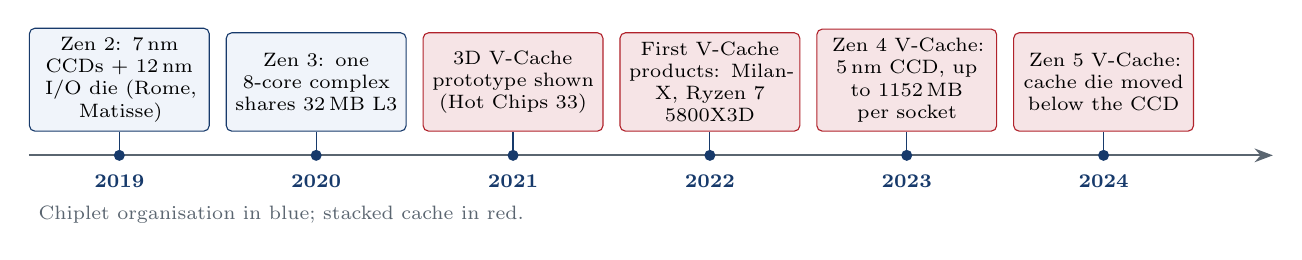
\begin{tikzpicture}[x=1cm,y=1cm,
  ev/.style={draw=draftblue,fill=draftlight,rounded corners=2pt,font=\scriptsize,align=center,text width=2.05cm,minimum height=1.25cm},
  ev3/.style={ev,fill=todored!12,draw=todored},
  yr/.style={font=\scriptsize\bfseries,text=draftblue}]
\draw[-{Stealth},thick,draftgray] (-0.4,0) -- (15.4,0);
\foreach \x/\y/\t/\s in {
  0.75/2019/{Zen~2: 7\,nm CCDs + 12\,nm I/O die (Rome, Matisse)}/ev,
  3.25/2020/{Zen~3: one 8-core complex shares 32\,MB L3}/ev,
  5.75/2021/{3D V-Cache prototype shown (Hot Chips~33)}/ev3,
  8.25/2022/{First V-Cache products: Milan-X, Ryzen~7 5800X3D}/ev3,
  10.75/2023/{Zen~4 V-Cache: 5\,nm CCD, up to 1152\,MB per socket}/ev3,
  13.25/2024/{Zen~5 V-Cache: cache die moved below the CCD}/ev3}{
  \fill[draftblue] (\x,0) circle (0.07);
  \node[yr,below] at (\x,-0.12) {\y};
  \node[\s,above] at (\x,0.3) {\t};
  \draw[draftblue] (\x,0.07) -- (\x,0.3);}
\node[font=\scriptsize,text=draftgray,anchor=west] at (-0.4,-0.75) {Chiplet organisation in blue; stacked cache in red.};
\end{tikzpicture}
\caption[The steps of AMD's Zen design studied in this paper]{The steps of AMD's Zen design studied in this paper, with the year each was disclosed or launched \cite{suggs2019zen2,naffziger2020chiplet,advancedmicrodevicesinc.AMDLaunchesAMD2020,swaminathanAdvancedPackagingEnabling2021,wuu2022vcache,larabelAMDEPYC7773X2022,alam2ndGeneration3D2024,advancedmicrodevicesinc.4thGenAMD2023,advancedmicrodevicesinc.GamingLegendContinues2024}.}
\label{fig:zen-timeline}
\end{figure}

\subsection{A thought experiment: one die or eight?}
\label{sec:thought-experiment}
Consider two ways to build a 64-core processor. Processor A places all 64 cores on one large die. Processor B places them on eight smaller dies of eight cores each, connected inside one package to a separate I/O die. Both offer 64 cores. Are they equally expensive to make? Do they communicate equally quickly? Can they use the same manufacturing process?

Using AMD's Zen~2 dimensions, with the compute dies at 74\,mm$^2$ each and a monolithic equivalent of $8 \times 74 = 592$\,mm$^2$ for the compute area alone, the later parts of this paper answer these questions (\cref{tab:thought-experiment}).

\begin{table}[htbp]
  \centering
  \caption[One die or eight: the 64-core thought experiment, answered from later sections]{One die or eight: the 64-core thought experiment, answered from later sections (model results are illustrative).}
  \label{tab:thought-experiment}
  \small
  \begin{tabularx}{\textwidth}{@{}>{\raggedright\arraybackslash}p{3.0cm}>{\raggedright\arraybackslash}X>{\raggedright\arraybackslash}X>{\raggedright\arraybackslash}p{1.7cm}@{}}
    \toprule
    \textbf{Question} & \textbf{A: one 64-core die} & \textbf{B: eight 8-core dies + I/O die} & \textbf{Where} \\
    \midrule
    Can it be built? & For 64 cores with I/O, beyond the maximum reticle size \cite{naffziger2020chiplet} & Yes; each die is small & \cref{sec:monolithic-limits} \\
    Modelled yield ($D_0 = 0.2$\,cm$^{-2}$) & 38\% & 87\% per compute die & \cref{sec:yield-cost} \\
    64-core sets per 300\,mm wafer & about 35 & about 95 & \cref{sec:process-specialisation} \\
    AMD's cost estimate & roughly 2$\times$ at 32 and 48 cores & 1$\times$ (reference) & \cref{fig:chiplet-cost-chart} \\
    Manufacturing process & everything on the newest node & cores on 7\,nm, I/O on cheaper 12\,nm & \cref{sec:ccd-iod} \\
    Communication & on-die network only & every memory access crosses a die-to-die link (AMD: under 9\,ns round trip \cite{naffziger2020chiplet}) & \cref{sec:d2d} \\
    Memory latency & not available for comparison & AMD reports Rome's average at about 0.81$\times$ that of its multi-die predecessor \cite{naffziger2020chiplet} & \cref{tab:numa-latency} \\
    Cache per core & one shared design choice & each die has its own L3; can be enlarged per die by stacking & Part~\ref{part:stacked-cache} \\
    \bottomrule
  \end{tabularx}
\end{table}

The answers are not all in favour of B. By AMD's account the full 64-core design could not be built as one die at all, and the models of Part~\ref{part:chiplets} make B far cheaper, but it pays for that with a die-to-die hop on every memory access and with caches that are private to each die. The rest of the paper examines both sides of this trade, and how 3D stacking changes the cache side of it.

\subsection{Two linked scaling problems}
\label{sec:two-problems}

The paper is organised around two related problems (\cref{fig:research-framework}).

\textbf{Problem 1: scaling processor resources beyond a single die.} If a product needs more cores, memory channels and I/O than one economical die can hold, the processor can be partitioned into \glspl{chiplet}\index{chiplet}. AMD's Zen~2-based products separate eight-core compute dies (CCDs) built on a 7\,nm process from an I/O die (IOD) built on a mature 12\,nm process \cite{naffziger2020chiplet,suggs2019zen2}.

\textbf{Problem 2: scaling cache capacity without spending planar die area.} A larger \gls{llc} can reduce costly trips to main memory, but on a planar die every extra megabyte of SRAM enlarges the die, lowers yield and lengthens wires. AMD's \gls{v-cache}\index{3D V-Cache} instead stacks an additional SRAM die on top of the compute die, expanding the Zen~3 L3 from 32\,MB to 96\,MB per CCD \cite{wuu2022vcache,amd2022epyc7003}.

The problems are linked: the chiplet organisation makes the CCD a small, self-contained compute die with its own L3, and that die is the natural host for a stacked cache. The paper therefore follows the argument in four steps:

\begin{enumerate}
  \item Monolithic CPUs face die-size, yield and scaling limits; chiplets address compute scaling \cite{naffziger2020chiplet}.
  \item Chiplets alone leave the cost of large on-die caches unsolved: AMD's ISSCC~2022 presentation names the slowing scaling and rising cost of SRAM as barriers to large on-die caches, in cost, product flexibility and latency, and argues that 2.5D chiplets address only part of the problem \cite[slides~6--7]{wuu2022vcache}.
  \item Vertical stacking addresses those cache-specific limits \cite{wuu2022vcache,swaminathanAdvancedPackagingEnabling2021}.
  \item Evaluation evidence shows where the stacked cache improves performance, and which thermal, packaging and cost trade-offs it introduces (Part~\ref{part:case-study}).
\end{enumerate}

\begin{figure}[htbp]
\centering
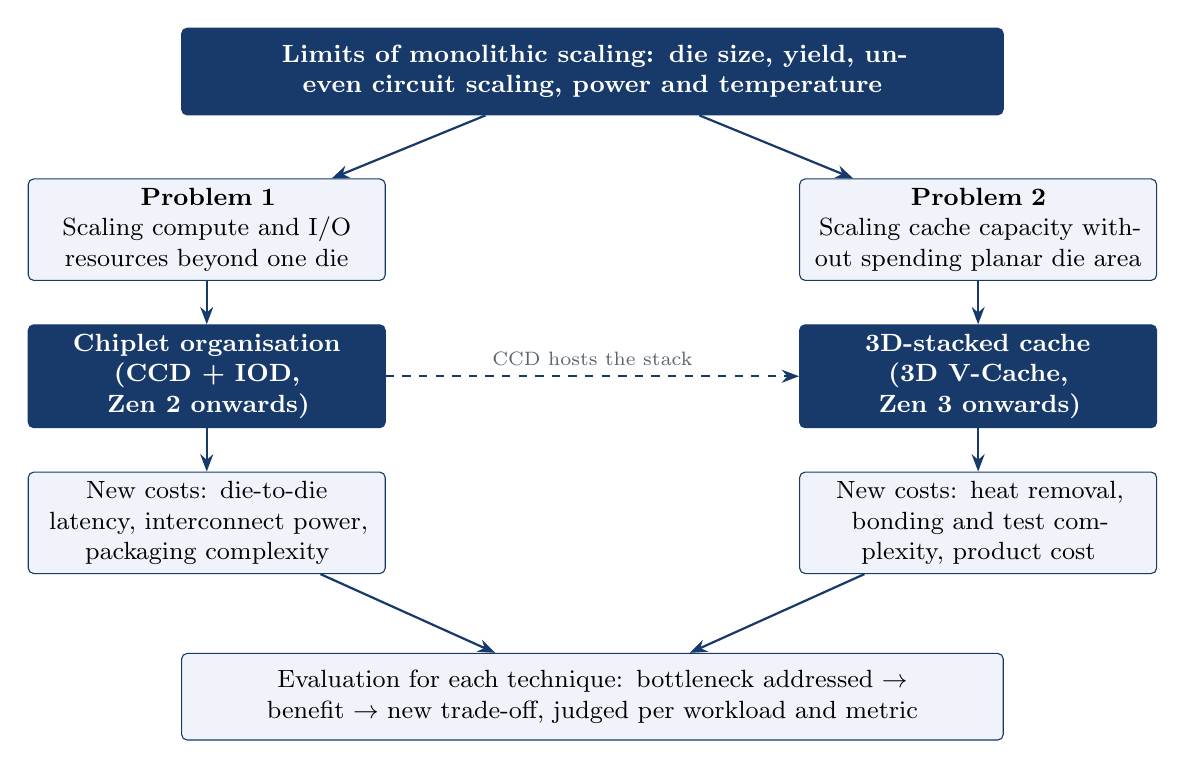
\begin{tikzpicture}[
  box/.style={draw=draftblue,fill=draftlight,rounded corners=2pt,align=center,text width=4.3cm,minimum height=1.1cm,font=\small},
  hdr/.style={box,fill=draftblue,text=white,font=\small\bfseries},
  arr/.style={-{Stealth[length=2.2mm]},draftblue,thick},
  node distance=0.55cm and 0.9cm]
\node[hdr,text width=10.2cm] (top) {Limits of monolithic scaling: die size, yield, uneven circuit scaling, power and temperature};
\node[box,below left=0.8cm and -2.6cm of top] (p1) {\textbf{Problem 1}\\Scaling compute and I/O resources beyond one die};
\node[box,below right=0.8cm and -2.6cm of top] (p2) {\textbf{Problem 2}\\Scaling cache capacity without spending planar die area};
\node[hdr,below=of p1] (s1) {Chiplet organisation\\(CCD + IOD, Zen 2 onwards)};
\node[hdr,below=of p2] (s2) {3D-stacked cache\\(3D V-Cache, Zen 3 onwards)};
\node[box,below=of s1] (t1) {New costs: die-to-die latency, interconnect power, packaging complexity};
\node[box,below=of s2] (t2) {New costs: heat removal, bonding and test complexity, product cost};
\node[box,below=1.0cm of $(t1.south)!0.5!(t2.south)$,text width=10.2cm] (q) {Evaluation for each technique: bottleneck addressed $\rightarrow$ benefit $\rightarrow$ new trade-off, judged per workload and metric};
\draw[arr] (top) -- (p1); \draw[arr] (top) -- (p2);
\draw[arr] (p1) -- (s1); \draw[arr] (p2) -- (s2);
\draw[arr] (s1) -- (t1); \draw[arr] (s2) -- (t2);
\draw[arr] (t1) -- (q); \draw[arr] (t2) -- (q);
\draw[arr,dashed] (s1) -- node[above,font=\scriptsize,text=draftgray]{CCD hosts the stack} (s2);
\end{tikzpicture}
\caption[Research framework]{Research framework: two linked scaling problems, the AMD responses studied in this paper, and the evaluation question applied to each.}
\label{fig:research-framework}
\end{figure}

\subsection{Research questions and objectives}
\label{sec:rq}

The central research question is:

\begin{quote}
\itshape How do chiplet-based organisation and 3D-stacked cache help modern processors address limits in performance, scalability, memory latency, power and die-level integration, and what new trade-offs do they introduce?
\end{quote}

It is divided into four sub-questions, the second with a supporting question:

\begin{description}[leftmargin=1.2cm,style=nextline]
  \item[RQ1] Which architectural and manufacturing limits make a single large die an increasingly costly way to scale a processor?
  \item[RQ2] How does partitioning a processor into compute and I/O dies change memory latency, bandwidth, power and product flexibility?
  \item[RQ2a] How does AMD divide processor functionality between the CCDs and the IOD, and why does it connect them through the organic package substrate rather than a 2.5D or 3D interconnect?
  \item[RQ3] Why does last-level-cache capacity matter, and what does vertical stacking change compared with expanding the cache in the plane of the die?
  \item[RQ4] For which workloads does a larger stacked L3 produce measurable benefit, and how can that benefit be separated from differences in frequency, core count and memory configuration?
\end{description}

For every technique the paper applies the same three-part test: \emph{which bottleneck does it address, what benefit does it provide, and what new bottleneck, cost or trade-off does it create?} \Cref{tab:rq-map} shows where each question is answered.

\begin{table}[htbp]
  \centering
  \caption[Where the research questions are answered]{Where the research questions are answered.}
  \label{tab:rq-map}
  \small
  \begin{tabularx}{\textwidth}{@{}lX>{\raggedright\arraybackslash}p{4.2cm}@{}}
    \toprule
    \textbf{Question} & \textbf{Main evidence} & \textbf{Sections} \\
    \midrule
    RQ1 & Reticle limit, yield and dies-per-wafer models, uneven scaling of circuit types & Part~\ref{part:chiplets} (\cref{sec:monolithic-limits,sec:yield-cost}); \cref{app:dies-per-wafer} \\
    RQ2, RQ2a & AMD's chiplet disclosures, die-to-die link figures, non-uniform memory access (NUMA) latencies, packaging options; the chiplet simulation & Part~\ref{part:chiplets} (\cref{sec:ccd-iod,sec:d2d,sec:packaging-options}); \cref{sec:sim-chiplet} \\
    RQ3 & Planar limits, hybrid bonding, the stacked-cache interface, thermal and manufacturing evidence; the simulated design comparison & Part~\ref{part:stacked-cache}; \cref{sec:sim-designs} \\
    RQ4 & AMD-reported and independent measurements, graded for confounding factors; the simulations & Part~\ref{part:case-study} (\cref{sec:sim-study}) \\
    All & Comparison, interactions and conclusions & Part~\ref{part:synthesis} \\
    \bottomrule
  \end{tabularx}
\end{table}

\Cref{fig:mindmap-rq} shows the same questions at a glance.

\mapfigure{%
\node[mmroot] (r) {Chiplets and stacked cache: what do they fix, and at what cost?};
\node[mmbox,mmlevel1,fill=mmF4AAA2] (b0) at (0.00,3.60) {RQ1\\Why one die is costly};
\draw[mmbig] (r) -- (b0);
\node[mmlevel2,mmbox,fill=mmCFE7E1] (b0c0) at (-3.05,5.35) {Yield and area};
\draw[mmsmall] (b0.north) to[out=90,in=-90] (b0c0.south);
\node[mmlevel2,mmbox,fill=mmCFE7E1] (b0c1) at (0.00,5.35) {Reticle limit};
\draw[mmsmall] (b0.north) to[out=90,in=-90] (b0c1.south);
\node[mmlevel2,mmbox,fill=mmCFE7E1] (b0c2) at (3.05,5.35) {Analog and SRAM scale poorly};
\draw[mmsmall] (b0.north) to[out=90,in=-90] (b0c2.south);
\node[mmbox,mmlevel1,fill=mmCFE7E1] (b1) at (4.47,1.36) {RQ2\\Compute and I/O dies};
\draw[mmbig] (r) -- (b1);
\node[mmlevel2,mmbox,fill=mmF9D7AF] (b1c0) at (8.07,2.81) {Memory latency};
\draw[mmsmall] (b1.east) to[out=0,in=180] (b1c0.west);
\node[mmlevel2,mmbox,fill=mmF9D7AF] (b1c1) at (8.07,1.36) {Bandwidth and power};
\draw[mmsmall] (b1.east) to[out=0,in=180] (b1c1.west);
\node[mmlevel2,mmbox,fill=mmF9D7AF] (b1c2) at (8.07,-0.09) {Product flexibility};
\draw[mmsmall] (b1.east) to[out=0,in=180] (b1c2.west);
\node[mmbox,mmlevel1,fill=mmCFE0F4] (b2) at (2.76,-3.56) {RQ2a\\How the dies connect};
\draw[mmbig] (r) -- (b2);
\node[mmlevel2,mmbox,fill=mmF9D7AF] (b2c0) at (6.36,-2.11) {Organic substrate};
\draw[mmsmall] (b2.east) to[out=0,in=180] (b2c0.west);
\node[mmlevel2,mmbox,fill=mmF9D7AF] (b2c1) at (6.36,-3.56) {2.5D interposer or bridge};
\draw[mmsmall] (b2.east) to[out=0,in=180] (b2c1.west);
\node[mmlevel2,mmbox,fill=mmF9D7AF] (b2c2) at (6.36,-5.01) {3D stacking};
\draw[mmsmall] (b2.east) to[out=0,in=180] (b2c2.west);
\node[mmbox,mmlevel1,fill=mmF9D7AF] (b3) at (-2.76,-3.56) {RQ3\\Why LLC capacity};
\draw[mmbig] (r) -- (b3);
\node[mmlevel2,mmoval,fill=mmDCCFF6] (b3c0) at (-6.36,-2.11) {Capacity misses};
\draw[mmsmall] (b3.west) to[out=180,in=0] (b3c0.east);
\node[mmlevel2,mmoval,fill=mmDCCFF6] (b3c1) at (-6.36,-3.56) {Planar limits};
\draw[mmsmall] (b3.west) to[out=180,in=0] (b3c1.east);
\node[mmlevel2,mmbox,fill=mmDCCFF6] (b3c2) at (-6.36,-5.01) {What stacking changes};
\draw[mmsmall] (b3.west) to[out=180,in=0] (b3c2.east);
\node[mmoval,mmlevel1,fill=mmDCCFF6] (b4) at (-4.47,1.36) {RQ4\\Where it helps};
\draw[mmbig] (r) -- (b4);
\node[mmlevel2,mmbox,fill=mmF4C2BB] (b4c0) at (-8.07,2.81) {Working set};
\draw[mmsmall] (b4.west) to[out=180,in=0] (b4c0.east);
\node[mmlevel2,mmbox,fill=mmF4C2BB] (b4c1) at (-8.07,1.36) {Frequency, cores, memory};
\draw[mmsmall] (b4.west) to[out=180,in=0] (b4c1.east);
\node[mmlevel2,mmbox,fill=mmF4C2BB] (b4c2) at (-8.07,-0.09) {Isolating the cache};
\draw[mmsmall] (b4.west) to[out=180,in=0] (b4c2.east);
}{[Overview of the research questions of \cref{sec:rq}]{Overview of the research questions of \cref{sec:rq}. Every branch is answered with the same test: which bottleneck the technique addresses, what it gains, and what new trade-off it creates.}}{fig:mindmap-rq}


\subsection{Scope}
\label{sec:scope}

AMD Zen processors are the principal case study because AMD has published unusually detailed technical descriptions of both its chiplet organisation and its stacked cache \cite{naffziger2020chiplet,suggs2019zen2,amd2022epyc7003,swaminathanAdvancedPackagingEnabling2021}. They are, however, a case study and not the whole subject: the architectural principles apply to chiplet and die-stacked designs in general.

The following are deliberately outside scope:

\begin{itemize}
  \item fabrication chemistry and process details beyond what is needed to explain an architectural decision;
  \item reverse engineering of undisclosed Zen internals;
  \item a catalogue of product specifications;
  \item vendor contests. Comparisons are always tied to a stated workload, metric and time period, and the paper makes no general claim that one vendor ``beats'' another.
\end{itemize}

\subsection{Related work}
\label{sec:related-work}
Earlier surveys cover each technique on its own. Liu, Li and Yin review chiplet-based design as a whole, dividing it into system architecture and interconnection. They identify as the main challenges the mapping of functions onto chiplets, the co-optimisation of package and architecture, the added latency of communication between dies, and keeping independently designed chiplets deadlock-free when they are combined \cite{liuReviewChipletbasedDesign2024}. Their review is broad and spans many vendors and accelerators, rather than tracing one product family through its generations. Mittal and Vetter survey techniques for building large last-level caches from DRAM, motivated by the low density and high leakage of SRAM \cite{mittalSurveyTechniquesArchitecting2016}. Their survey predates hybrid-bonded SRAM stacking in products, so it treats a different technology from the one AMD chose (\cref{sec:sram}). At the level of individual designs, Black \emph{et al.} simulated stacking SRAM and DRAM caches on a processor in 2006, including their thermal cost \cite{blackStacking3DMicroarchitecture2006}, and Dong and Xie built a system-level cost model for 3D integrated circuits, which finds that stacking pays only above a certain design size \cite{dongSystemlevelCostAnalysis2009}. Domke \emph{et al.} come closest to this paper's subject. They measured Milan-X against Milan on high-performance computing (HPC) proxy applications, and simulated a hypothetical future processor with very large stacked SRAM, reporting an average 9.56$\times$ per-chip gain for cache-sensitive HPC applications \cite{domkeLocusPerformanceQuantifying2023}. Their focus is HPC and future designs, not the trade-offs of the products already shipped.

This paper differs from these works in three ways. It treats chiplets and stacked cache as two answers to related limits of one design, the AMD Zen family. It explains both with the models of an undergraduate textbook, so that each claim can be checked by hand. And it grades the published evidence by what each comparison controls, rather than quoting headline figures.

\subsection{Methodology}
\label{sec:method-overview}

The study combines five kinds of evidence:

\begin{enumerate}
  \item \textbf{Textbook foundations.} Chapters 7 and 9--12 of Sarangi's \emph{Basic Computer Architecture} supply the models used throughout. The topic maps mainly to Chapters 11 (the memory system) and 12 (multiprocessors), with foundations from Chapters 7, 9 and 10; all lie within Chapters 1--12, so the faculty advisor is Prof. Sumantra Dutta Roy. The models used are the performance equation, pipelining limits, power and temperature, the memory hierarchy and average memory access time, and multicore coherence and interconnects \cite{sarangi2025basic}.
  \item \textbf{Primary technical disclosures.} Peer-reviewed conference papers and vendor technical presentations describe what was built and why. Vendor presentations are attributed to the vendor and treated as engineering claims rather than independent measurements.
  \item \textbf{Published research and benchmarks.} Part~\ref{part:case-study} analyses published measurements of chiplet and stacked-cache processors. Apart from the one set of measurements on a single-CCD part described below, the paper performs no new measurements of these processors; its quantitative contribution lies in organising, normalising and critically comparing existing results (\cref{sec:evidence-method}).
  \item \textbf{A simulation.} A trace-driven model of the cache hierarchy, built by the group and calibrated against published measurements, changes one factor at a time where no published comparison does (\cref{sec:sim-study}). Its results are labelled as model outputs throughout.
  \item \textbf{The group's own measurements.} Latency, overlap of misses, bandwidth and core-to-core tests on the group's Ryzen~5 5600X, a single-CCD Zen~3 chiplet processor without stacked cache, compare the model with a machine it was not built from (\cref{app:5600x}).
\end{enumerate}

Two practices run through the analysis. First, \emph{calculations} apply the textbook's models to published numbers: yield and cost per wafer, connection density, average memory access time, the stacked-cache trade-off and clock correction. Each states its inputs, and any assumed value is labelled as such. Second, sources are graded. Vendor presentations are used for what was built; independent measurements, preferably with fixed clocks or performance counters, are used for what it achieves; and where a value had to be read from a published chart rather than a table, the text says so and gives the reading accuracy.

\subsection{Contributions}
\label{sec:contributions}

This paper makes no new measurements of stacked-cache processors or of traffic between CCDs, and one set on a Ryzen~5 5600X, a single-CCD chiplet part without stacked cache; its contributions are otherwise analytical and, in one part, computational:
\begin{itemize}
  \item a single argument linking chiplet partitioning and 3D-stacked cache as responses to two related scaling limits, die cost and last-level cache capacity;
  \item an explanation of both techniques in terms of the textbook's performance, power, thermal and memory-hierarchy models;
  \item a structured comparison of planar, side-by-side and vertically stacked cache expansion;
  \item a synthesis of AMD-reported and independent performance evidence for stacked cache across three Zen generations, graded by which confounding factors each comparison controls (\cref{tab:confound-grid});
  \item an account of how AMD's move to an inverted stack in Zen~5 bears on the thermal cost of the first design;
  \item seven simulations, most changing one factor at a time, with the model, scripts and raw results on GitHub for repetition (\href{\repourl}{\nolinkurl{\repourlshort}}; \cref{sec:sim-study,app:sim-setup});
  \item measurements on the group's own Ryzen~5 5600X, compared with the model on a machine it was not built from (\cref{sec:sim-calibration,app:5600x}).
\end{itemize}

\subsection{Main findings}
\label{sec:findings}
The main findings, each developed in the part cited, are as follows.
\begin{itemize}
  \item \textbf{Chiplets trade a small latency cost on every L3 miss for cost and flexibility.} Smaller dies yield far better, I/O moves to a cheaper node (\cref{sec:yield-cost}), and within each generation one compute die serves a wide range of products, from desktop parts to 64-core (Zen~3) or 96-core (Zen~4) servers (\cref{sec:product-flexibility}). Every L3 miss pays a die-to-die round trip that AMD gives as under 9\,ns, yet AMD reports that Rome's average memory latency was 19\% lower than its predecessor's (\cref{sec:d2d}). The largest cost is in sharing: in the one measurement available, passing data between cores on different CCDs took about 4.5 times as long as within one (\cref{sec:cross-ccd}). The power cost can only be estimated, at about 2\% of a Genoa processor's power budget for memory traffic alone (\cref{sec:chiplet-power}).
  \item \textbf{Stacking triples the L3 for about four cycles.} AMD's first cache die expands a Zen~3 CCD's L3 from 32 to 96\,MB for about four extra cycles of latency, a cost measured in three generations by one independent outlet (Part~\ref{part:stacked-cache}, \cref{sec:milanx-latency}).
  \item \textbf{The benefit depends on the working set.} At equal clock, the best-controlled study finds gains in instructions per cycle (IPC) of 4.9--19.7\% in five workloads, a geometric mean of 11.4\% by the authors' calculation, and a small loss in a sixth (\cref{sec:lam-detail}). Memory-bound computational fluid dynamics (OpenFOAM) gains up to 1.5--1.6$\times$ and one HPC proxy up to 3.4$\times$ at favourable problem sizes, while working sets that already fit gain nothing (Part~\ref{part:case-study}).
  \item \textbf{A removed miss is worth less than a memory access.} In the measured workloads each counted miss removed was worth an apparent 50 to 130 cycles, well below the memory latency. Overlap of misses by out-of-order cores and the counting of prefetches as misses are two candidate explanations; the sources do not separate them (\cref{sec:tradeoff-example,sec:lam-detail}).
  \item \textbf{Lower clocks offset part of the gain.} In the first two generations the V-Cache parts clocked lower. A simple model calibrated on published measurements shows that a 7\% clock gap raises the number of misses the larger cache must remove to break even from about 0.1 to about 0.35 per thousand instructions. The simulation, built on the same calibration and so not an independent check, gives 0.38 at that gap (\cref{sec:cache-clock-model,sec:sim-clock}).
  \item \textbf{A simulation illustrates these mechanisms.} A trace-driven cache model, calibrated on the same measurements, reproduces the working-set window, the small latency cost and the weight of the clock gap with every other factor fixed. It also shows which inputs matter: across the overlap factors fitted to Lam's workloads the break-even at a realistic clock gap changes about threefold, and the two link round trips of one transfer between CCDs explain only part of the measured cost of sharing (\cref{sec:sim-study}). Its results are model outputs, not measurements.
  \item \textbf{The group's own measurements check the model's inputs and expose its limits.} On a Ryzen~5 5600X, the published Zen~3 L1 and L2 latencies the model uses agree with the measured ones, and its L3 and memory latencies are within about 20\%. The core keeps at least sixteen misses in flight, enough for the overlap the calibration implies. Between the cache plateaus, where the model's own behaviour shows, its latency close to each cache's capacity is too low, by up to 2.4 times (at 32\,MB, measured under the Windows Subsystem for Linux, WSL2; \cref{sec:sim-calibration}).
\end{itemize}

\subsection{Organisation of the paper}
\label{sec:organisation}

Part~\ref{part:foundations} reviews the architectural foundations. Part~\ref{part:chiplets} analyses chiplet-based organisation. Part~\ref{part:stacked-cache} examines 3D-stacked cache and AMD 3D V-Cache. Part~\ref{part:case-study} presents the AMD case study and quantitative analysis, and Part~\ref{part:synthesis} compares the approaches, identifies limitations and outlines future directions. Self-contained derivations longer than about half a page appear as appendices. \Cref{fig:mindmap-paper} maps the whole paper.

\mapfigure{%
\node[mmroot] (r) {Scaling beyond one large die};
\node[mmbox,mmlevel1,fill=mmF4AAA2] (b0) at (0.00,3.60) {Monolithic limits\\(Parts I, III)};
\draw[mmbig] (r) -- (b0);
\node[mmlevel2,mmbox,fill=mmCFE7E1] (b0c0) at (-3.05,5.35) {Yield falls with area};
\draw[mmsmall] (b0.north) to[out=90,in=-90] (b0c0.south);
\node[mmlevel2,mmbox,fill=mmCFE7E1] (b0c1) at (0.00,5.35) {Reticle limit};
\draw[mmsmall] (b0.north) to[out=90,in=-90] (b0c1.south);
\node[mmlevel2,mmbox,fill=mmCFE7E1] (b0c2) at (3.05,5.35) {Uneven node scaling};
\draw[mmsmall] (b0.north) to[out=90,in=-90] (b0c2.south);
\node[mmbox,mmlevel1,fill=mmCFE0F4] (b1) at (4.07,2.20) {Foundations\\(Part II)};
\draw[mmbig] (r) -- (b1);
\node[mmlevel2,mmbox,fill=mmF9D7AF] (b1c0) at (7.67,3.65) {AMAT and miss classes};
\draw[mmsmall] (b1.east) to[out=0,in=180] (b1c0.west);
\node[mmlevel2,mmbox,fill=mmF9D7AF] (b1c1) at (7.67,2.20) {Coherence};
\draw[mmsmall] (b1.east) to[out=0,in=180] (b1c1.west);
\node[mmlevel2,mmbox,fill=mmF9D7AF] (b1c2) at (7.67,0.75) {Power and heat};
\draw[mmsmall] (b1.east) to[out=0,in=180] (b1c2.west);
\node[mmbox,mmlevel1,fill=mmCFE7E1] (b2) at (4.07,-2.20) {Chiplets\\(Part III)};
\draw[mmbig] (r) -- (b2);
\node[mmlevel2,mmbox,fill=mmF9D7AF] (b2c0) at (7.67,-0.75) {CCD and I/O die};
\draw[mmsmall] (b2.east) to[out=0,in=180] (b2c0.west);
\node[mmlevel2,mmbox,fill=mmF9D7AF] (b2c1) at (7.67,-2.20) {Package links, NUMA};
\draw[mmsmall] (b2.east) to[out=0,in=180] (b2c1.west);
\node[mmlevel2,mmbox,fill=mmF9D7AF] (b2c2) at (7.67,-3.65) {Cost per good die};
\draw[mmsmall] (b2.east) to[out=0,in=180] (b2c2.west);
\node[mmbox,mmlevel1,fill=mmF9D7AF] (b3) at (0.00,-3.60) {Stacked cache\\(Part IV)};
\draw[mmbig] (r) -- (b3);
\node[mmlevel2,mmoval,fill=mmDCCFF6] (b3c0) at (-3.05,-5.35) {Hybrid bonding};
\draw[mmsmall] (b3.south) to[out=-90,in=90] (b3c0.north);
\node[mmlevel2,mmbox,fill=mmDCCFF6] (b3c1) at (0.00,-5.35) {3$\times$ L3 for 4 cycles};
\draw[mmsmall] (b3.south) to[out=-90,in=90] (b3c1.north);
\node[mmlevel2,mmoval,fill=mmDCCFF6] (b3c2) at (3.05,-5.35) {Heat path};
\draw[mmsmall] (b3.south) to[out=-90,in=90] (b3c2.north);
\node[mmoval,mmlevel1,fill=mmDCCFF6] (b4) at (-4.07,-2.20) {Evidence\\(Part V)};
\draw[mmbig] (r) -- (b4);
\node[mmlevel2,mmbox,fill=mmF4C2BB] (b4c0) at (-7.67,-0.75) {Fixed-clock IPC};
\draw[mmsmall] (b4.west) to[out=180,in=0] (b4c0.east);
\node[mmlevel2,mmbox,fill=mmF4C2BB] (b4c1) at (-7.67,-2.20) {Working-set sweeps};
\draw[mmsmall] (b4.west) to[out=180,in=0] (b4c1.east);
\node[mmlevel2,mmbox,fill=mmF4C2BB] (b4c2) at (-7.67,-3.65) {Cache against clock; simulation};
\draw[mmsmall] (b4.west) to[out=180,in=0] (b4c2.east);
\node[mmbox,mmlevel1,fill=mmD6EBC6] (b5) at (-4.07,2.20) {Synthesis\\(Part VI)};
\draw[mmbig] (r) -- (b5);
\node[mmlevel2,mmoval,fill=mmDCCFF6] (b5c0) at (-7.67,3.65) {Strength of evidence};
\draw[mmsmall] (b5.west) to[out=180,in=0] (b5c0.east);
\node[mmlevel2,mmoval,fill=mmDCCFF6] (b5c1) at (-7.67,2.20) {Bandwidth wall};
\draw[mmsmall] (b5.west) to[out=180,in=0] (b5c1.east);
\node[mmlevel2,mmoval,fill=mmDCCFF6] (b5c2) at (-7.67,0.75) {Future integration};
\draw[mmsmall] (b5.west) to[out=180,in=0] (b5c2.east);
}{[Overview of the paper]{Overview of the paper: the problem at the centre, one branch per part, and the main idea each part contributes.}}{fig:mindmap-paper}

\clearpage
\part{Architectural Foundations}
\label{part:foundations}
\Cref{fig:mindmap-foundations} maps the topics of this part.

\mapfigure{%
\node[mmroot] (r) {Architectural foundations};
\node[mmbox,mmlevel1,fill=mmCFE0F4] (b0) at (0.00,3.60) {Performance};
\draw[mmbig] (r) -- (b0);
\node[mmlevel2,mmbox,fill=mmF9D7AF] (b0c0) at (-1.52,5.35) {IPC $\times f$ / instructions};
\draw[mmsmall] (b0.north) to[out=90,in=-90] (b0c0.south);
\node[mmlevel2,mmbox,fill=mmF9D7AF] (b0c1) at (1.52,5.35) {Baseline organisation};
\draw[mmsmall] (b0.north) to[out=90,in=-90] (b0c1.south);
\node[mmbox,mmlevel1,fill=mmF4AAA2] (b1) at (4.47,1.36) {Pipelining, power, heat};
\draw[mmbig] (r) -- (b1);
\node[mmlevel2,mmbox,fill=mmCFE7E1] (b1c0) at (8.07,2.81) {Pipeline depth};
\draw[mmsmall] (b1.east) to[out=0,in=180] (b1c0.west);
\node[mmlevel2,mmbox,fill=mmCFE7E1] (b1c1) at (8.07,1.36) {Dynamic and leakage power};
\draw[mmsmall] (b1.east) to[out=0,in=180] (b1c1.west);
\node[mmlevel2,mmbox,fill=mmCFE7E1] (b1c2) at (8.07,-0.09) {Thermal resistance};
\draw[mmsmall] (b1.east) to[out=0,in=180] (b1c2.west);
\node[mmbox,mmlevel1,fill=mmCFE7E1] (b2) at (2.76,-3.56) {Memory hierarchy};
\draw[mmbig] (r) -- (b2);
\node[mmlevel2,mmbox,fill=mmF9D7AF] (b2c0) at (6.36,-2.11) {SRAM and DRAM};
\draw[mmsmall] (b2.east) to[out=0,in=180] (b2c0.west);
\node[mmlevel2,mmbox,fill=mmF9D7AF] (b2c1) at (6.36,-3.56) {AMAT};
\draw[mmsmall] (b2.east) to[out=0,in=180] (b2c1.west);
\node[mmlevel2,mmbox,fill=mmF9D7AF] (b2c2) at (6.36,-5.01) {Miss classes};
\draw[mmsmall] (b2.east) to[out=0,in=180] (b2c2.west);
\node[mmbox,mmlevel1,fill=mmF9D7AF] (b3) at (-2.76,-3.56) {Cache design};
\draw[mmbig] (r) -- (b3);
\node[mmlevel2,mmoval,fill=mmDCCFF6] (b3c0) at (-6.36,-2.11) {Sets and ways};
\draw[mmsmall] (b3.west) to[out=180,in=0] (b3c0.east);
\node[mmlevel2,mmbox,fill=mmDCCFF6] (b3c1) at (-6.36,-3.56) {Replacement and write policy};
\draw[mmsmall] (b3.west) to[out=180,in=0] (b3c1.east);
\node[mmlevel2,mmbox,fill=mmDCCFF6] (b3c2) at (-6.36,-5.01) {Other LLC technologies};
\draw[mmsmall] (b3.west) to[out=180,in=0] (b3c2.east);
\node[mmoval,mmlevel1,fill=mmDCCFF6] (b4) at (-4.47,1.36) {Multicore};
\draw[mmbig] (r) -- (b4);
\node[mmlevel2,mmbox,fill=mmF4C2BB] (b4c0) at (-8.07,2.81) {Amdahl's law};
\draw[mmsmall] (b4.west) to[out=180,in=0] (b4c0.east);
\node[mmlevel2,mmbox,fill=mmF4C2BB] (b4c1) at (-8.07,1.36) {Coherence: MSI, directory};
\draw[mmsmall] (b4.west) to[out=180,in=0] (b4c1.east);
\node[mmlevel2,mmbox,fill=mmF4C2BB] (b4c2) at (-8.07,-0.09) {Interconnect topologies};
\draw[mmsmall] (b4.west) to[out=180,in=0] (b4c2.east);
}{[Overview of Part~\ref{part:foundations}]{Overview of Part~\ref{part:foundations}: the textbook concepts that the later parts use to judge chiplets and stacked cache.}}{fig:mindmap-foundations}

This part sets out the models that the rest of the paper uses to judge chiplets and stacked cache. It follows Chapters 7 and 9--12 of the course textbook \cite{sarangi2025basic}. The textbook supplies the theory; it does not describe modern compute-die/I/O-die partitioning or stacked cache, which later parts support with external sources.

\section{Processor Organisation and Performance Metrics}
\label{sec:perf-metrics}

\subsection{The performance equation}

The textbook defines the performance of a processor only with respect to a given program, as the reciprocal of its execution time \cite[sec.~10.9.1]{sarangi2025basic}. Execution time $\tau$ can be split into three factors:
\begin{equation}
  \tau \;=\; \frac{\#\text{instructions} \times \mathrm{CPI}}{f},
  \qquad
  P \;\propto\; \frac{\mathrm{IPC} \times f}{\#\text{instructions}},
  \label{eq:perf}
\end{equation}
where $f$ is the clock frequency, \gls{cpi} is the average number of cycles per dynamic instruction, and \gls{ipc} is its reciprocal \cite[sec.~10.9.1]{sarangi2025basic}.\index{performance equation}

\Cref{eq:perf} is the lens for the whole paper. A larger cache does not change the instruction count or, directly, the clock frequency; it acts through IPC by reducing the cycles spent waiting for memory. A chiplet organisation, by contrast, can change all three: it can enable more cores (more throughput), alter memory latency (IPC), and change the frequency and power each die can sustain. When published results compare two processors, they must therefore be checked for differences in $f$ as well as in cache size (\cref{sec:confounds}).

\subsection{Baseline processor organisation}
The textbook builds its baseline processor, SimpleRisc, from five stages: instruction fetch (IF), operand fetch (OF), execute (EX), memory access (MA) and register writeback (RW) \cite[sec.~9.9.1]{sarangi2025basic}. The \emph{data path} holds and processes information (registers, memory elements, the ALU), while the \emph{control path} generates the signals that move instructions and data through it; the control path can be a hardwired control unit or a microprogrammed one, which trades speed for flexibility \cite[secs.~9.2--9.8]{sarangi2025basic}.

Two features of this baseline matter for the rest of the paper. First, the MA stage is the processor's only contact with memory: every load and store passes through it, so the speed of the memory system directly sets how long that stage can take. Second, the organisation assumes a single processor on a single piece of silicon. Everything that follows, from pipelining to multicore processors and finally to chiplets, can be read as a series of departures from this baseline, each made to use a larger transistor budget without lengthening the clock cycle or exceeding the power budget.

\section{Pipelining, Power and Thermal Limits}
\label{sec:pipelining-power}

\subsection{Pipelining and its limits}
In the basic processor, most of the hardware is idle at any moment: when an instruction is in the MA stage, the IF stage has nothing to do. Pipelining overlaps instructions so that each of the five stages works on a different instruction in the same cycle, with pipeline registers between stages carrying each instruction's state forward \cite[sec.~10.12.1]{sarangi2025basic}. Ideally this completes one instruction per cycle while allowing the clock frequency to rise roughly in proportion to the number of stages.

The ideal is broken by \emph{hazards}. A data (read-after-write) hazard occurs when an instruction needs a value that an earlier instruction has not yet produced; a control hazard occurs because the outcome of a branch is not known when the following instructions are fetched; a structural hazard occurs when two instructions need the same hardware unit \cite[sec.~10.4]{sarangi2025basic}. Interlocks resolve hazards by stalling, and forwarding passes results directly between stages, which removes every data hazard except the load-use hazard \cite[sec.~10.12.1]{sarangi2025basic}. The effect on performance is captured by
\begin{equation}
  \mathrm{CPI} = \mathrm{CPI}_{\mathrm{ideal}} + \text{stall rate} \times \text{stall penalty},
  \label{eq:cpi-stalls}
\end{equation}
so the CPI grows with every stall cycle. Deeper pipelines raise the frequency but also the stall penalty, which is why the textbook derives an optimal pipeline depth rather than an unlimited one \cite[sec.~10.9.3]{sarangi2025basic}.

The textbook's model of pipeline depth \cite[sec.~10.9.3]{sarangi2025basic} finds an optimum of about 13 stages for typical values and draws three conclusions: programs with many dependencies favour shallower pipelines, better forwarding favours deeper ones, and the optimal depth has changed little over time because logic and latches have been getting faster at about the same rate. Deepening pipelines therefore has limits of its own, besides the power limit that ended the growth in clock frequency (\cref{sec:intro}). In our reading, a design that reduces the stall rate, such as a larger cache that removes memory stalls, is a useful alternative to a higher clock.

\Cref{eq:cpi-stalls} is the link between pipelining and the memory hierarchy. A load that misses in the cache is a stall whose penalty is not one or two cycles but the miss penalty of \cref{eq:amat}, which can be tens or hundreds of cycles. Out-of-order processors soften this: they fetch and decode in order, rename registers to remove false dependencies, and issue any instruction whose operands are ready from an instruction window that typically holds 64--128 entries \cite[sec.~10.11.4]{sarangi2025basic}. Independent work can therefore proceed while a load waits. But the window is finite, so a long miss to main memory eventually fills it and stalls the pipeline. Reducing the number of such misses, which is what a larger last-level cache does, therefore still matters even for aggressive out-of-order cores.

\subsection{Dynamic and leakage power}
\label{sec:power}

The textbook models dynamic power, the energy dissipated when circuit nodes switch, as
\begin{equation}
  P_{\mathrm{dyn}} \;\propto\; \sum_{i} \alpha_i\, C_i\, V^2 f,
  \label{eq:pdyn}
\end{equation}
where $\alpha_i$ is the activity factor and $C_i$ the capacitance of node $i$, $V$ the supply voltage and $f$ the frequency \cite[sec.~10.10.2]{sarangi2025basic}. Leakage (static) power arises because transistors do not switch off perfectly; it is consumed all the time regardless of activity, and the textbook notes that it can account for roughly 20--40\% of a high-performance processor's power budget \cite[sec.~10.10.3]{sarangi2025basic}.\index{leakage power}\index{dynamic power}

Both terms matter for this paper:
\begin{itemize}
  \item \textbf{Wires are capacitance.} Long on-die or die-to-die wires increase $C$ in \cref{eq:pdyn}, so moving data farther costs energy as well as time. This is one reason the distance between cores and cache matters (\cref{sec:planar-limits}).
  \item \textbf{Large SRAM arrays leak.} A large cache adds leakage even when most of it is idle, which is part of the cost of simply growing the LLC on a planar die.
\end{itemize}

\subsection{Temperature}
Power that is dissipated becomes heat, which must flow from the transistors through the die, a thermal interface material and a heat spreader to the cooler \cite[sec.~10.10.1]{sarangi2025basic} (\cref{fig:package-thermal}). The textbook gives a sense of the scale: a 200--400\,mm$^2$ die dissipating 60--100\,W would heat up to around 200\,\textdegree C without these measures, and even with them processors run at 60--100\,\textdegree C, reaching 120\,\textdegree C under heavy load \cite[sec.~10.10.1]{sarangi2025basic}.

\begin{figure}[htbp]
\centering
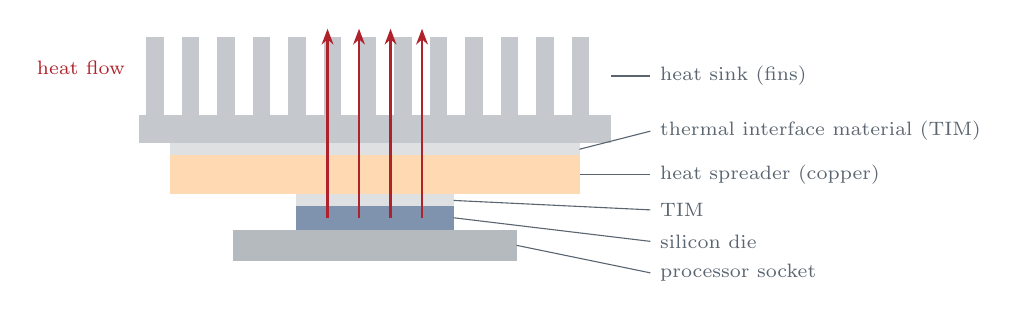
\begin{tikzpicture}[x=1cm,y=1cm,lab/.style={font=\scriptsize,anchor=west}]
\fill[draftgray!35] (1.0,3.25) rectangle (7.0,3.6);
\foreach \x in {1.1,1.55,...,6.9}{\fill[draftgray!35] (\x,3.6) rectangle (\x+0.22,4.6);}
\fill[draftgray!20] (1.4,3.1) rectangle (6.6,3.25);
\fill[orange!30] (1.4,2.6) rectangle (6.6,3.1);
\fill[draftgray!20] (3.0,2.45) rectangle (5.0,2.6);
\fill[draftblue!55] (3.0,2.15) rectangle (5.0,2.45);
\fill[draftgray!45] (2.2,1.75) rectangle (5.8,2.15);
\foreach \x in {3.4,3.8,4.2,4.6}{\draw[-{Stealth[length=2mm]},todored,thick] (\x,2.3) -- (\x,4.7);}
\draw[draftgray] (7.0,4.1) -- (7.5,4.1) node[lab]{heat sink (fins)};
\draw[draftgray] (6.6,3.17) -- (7.5,3.4) node[lab]{thermal interface material (TIM)};
\draw[draftgray] (6.6,2.85) -- (7.5,2.85) node[lab]{heat spreader (copper)};
\draw[draftgray] (5.0,2.52) -- (7.5,2.4) node[lab]{TIM};
\draw[draftgray] (5.0,2.3) -- (7.5,2.0) node[lab]{silicon die};
\draw[draftgray] (5.8,1.95) -- (7.5,1.6) node[lab]{processor socket};
\node[font=\scriptsize,text=todored,anchor=east] at (0.95,4.2) {heat flow};
\end{tikzpicture}
\caption[The heat path from a processor die to the air, redrawn after Sarangi]{The heat path from a processor die to the air, redrawn after Sarangi \cite[sec.~10.10.1, Fig.~10.36]{sarangi2025basic}. Each layer adds thermal resistance; stacking a second die on the processor adds another layer between the transistors and the spreader (\cref{sec:thermal}).}
\label{fig:package-thermal}
\end{figure}
 Higher temperature raises leakage, which raises power further, and accelerates ageing \cite[sec.~10.10.1]{sarangi2025basic}. Stacking a die on top of a compute die changes this heat path, which is the main thermal question raised in \cref{sec:thermal}.

Heat is not produced evenly. The textbook notes that the ALUs dissipate a lot of heat while memory elements stay relatively cool, and that the heat spreader exists to even out the resulting hot spots \cite[sec.~10.10.1]{sarangi2025basic}. It models the steady-state temperature by dividing the die into a grid of $m$ points:
\begin{equation}
  T - T_{\mathrm{amb}} \;=\; \Delta T \;=\; A \times P_{\mathrm{tot}},
  \label{eq:thermal}
\end{equation}
where $P_{\mathrm{tot}}$ is the vector of power dissipated at each grid point, $T_{\mathrm{amb}}$ the ambient temperature and $A$ the $m\times m$ \emph{thermal resistance matrix} \cite[sec.~10.10.4]{sarangi2025basic}.\index{thermal resistance} Because $P_{\mathrm{tot}} = P_{\mathrm{dyn}} + P_{\mathrm{leak}}$ and leakage itself grows with temperature, \cref{eq:thermal} and the leakage model form a feedback loop that must be iterated until it converges \cite[sec.~10.10.4]{sarangi2025basic}. Two consequences follow for stacking. Placing an extra layer over a hot region increases the entries of $A$ for that region, so the same power produces a higher temperature. A cool structure such as a cache array is the cheaper thing to put in the heat path. 3D V-Cache follows both rules: its cache die sits over the CCD's L3, and only structural silicon covers the cores (\cref{sec:thermal}).

\section{The Memory Hierarchy}
\label{sec:memory-hierarchy}

\subsection{Why a hierarchy is needed}

The textbook frames memory design as a conflict between capacity and speed. Per unit of silicon, DRAM stores far more data than SRAM but is much slower; a memory built entirely of DRAM would make every load and store wait for main memory, while a memory built entirely of fast on-chip SRAM cannot hold a program's data \cite[sec.~11.1.1]{sarangi2025basic}.\index{memory hierarchy}

The way out is \emph{locality}: programs tend to reuse recently used data (temporal locality) and to access data near recently used data (spatial locality) \cite[sec.~11.1.2--11.1.6]{sarangi2025basic}. A \gls{memory-hierarchy} keeps recently used blocks in small, fast caches close to the core and backs them with progressively larger, slower levels (\cref{fig:memory-hierarchy-amat}).

\begin{figure}[htbp]
\centering
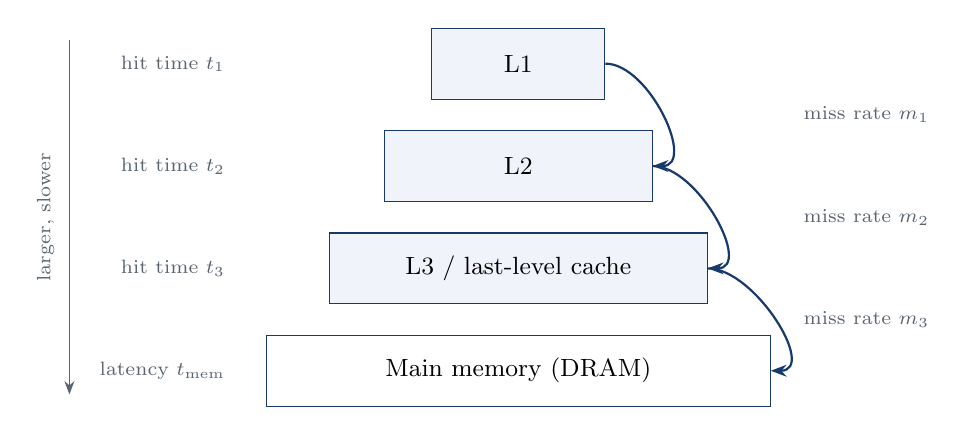
\begin{tikzpicture}[
  lvl/.style={draw=draftblue,fill=draftlight,align=center,minimum height=0.9cm,font=\small},
  arr/.style={-{Stealth[length=2mm]},draftblue,thick},
  note/.style={font=\scriptsize,text=draftgray,align=left}]
\node[lvl,minimum width=2.2cm] (l1) at (0,0) {L1};
\node[lvl,minimum width=3.4cm] (l2) at (0,-1.3) {L2};
\node[lvl,minimum width=4.8cm] (l3) at (0,-2.6) {L3 / last-level cache};
\node[lvl,minimum width=6.4cm,fill=white] (mm) at (0,-3.9) {Main memory (DRAM)};
\draw[arr] (l1.east) to[out=0,in=0] (l2.east);
\node[note,anchor=west] at (3.5,-0.65) {miss rate $m_1$};
\draw[arr] (l2.east) to[out=0,in=0] (l3.east);
\node[note,anchor=west] at (3.5,-1.95) {miss rate $m_2$};
\draw[arr] (l3.east) to[out=0,in=0] (mm.east);
\node[note,anchor=west] at (3.5,-3.25) {miss rate $m_3$};
\node[note,anchor=east] at (-3.6,0) {hit time $t_1$};
\node[note,anchor=east] at (-3.6,-1.3) {hit time $t_2$};
\node[note,anchor=east] at (-3.6,-2.6) {hit time $t_3$};
\node[note,anchor=east] at (-3.6,-3.9) {latency $t_{\mathrm{mem}}$};
\draw[draftgray,-{Stealth}] (-5.7,0.3) -- node[note,rotate=90,anchor=south,yshift=2pt]{larger, slower} (-5.7,-4.2);
\end{tikzpicture}
\caption[A multi-level cache hierarchy and the AMAT quantities]{A multi-level cache hierarchy with the quantities used in the recursive AMAT expression (\cref{eq:amat}). Capacity grows and speed falls moving down the hierarchy.}
\label{fig:memory-hierarchy-amat}
\end{figure}

\subsection{SRAM and DRAM arrays}
\label{sec:sram}
Caches are built from SRAM. A standard SRAM cell uses six transistors: two cross-coupled inverters hold the bit, and two access transistors, switched by a shared \emph{word line}, connect it to a pair of complementary \emph{bit lines} \cite[sec.~7.4.1]{sarangi2025basic}\index{SRAM}. Cells are laid out as a two-dimensional array: a decoder raises one word line, every cell in that row drives its bit lines, and a column multiplexer selects the bits of interest \cite[sec.~7.4.1]{sarangi2025basic}. Because hundreds of cells share a bit line, the bit line has a high capacitance and would be slow to charge fully. Reads therefore pre-charge both bit lines to half the supply voltage and let \emph{sense amplifiers} detect a small voltage difference \cite[sec.~7.4.1]{sarangi2025basic}. The textbook also notes that as an array grows it must be kept roughly square, otherwise the capacitive load on its word lines or bit lines becomes prohibitive \cite[sec.~7.4.1]{sarangi2025basic}. Large caches are therefore built as many smaller arrays and banks (\cref{sec:multicore}), connected by wires whose length grows with total capacity. \Cref{fig:sram-array} shows the cell and the array.

\begin{figure}[htbp]
\centering
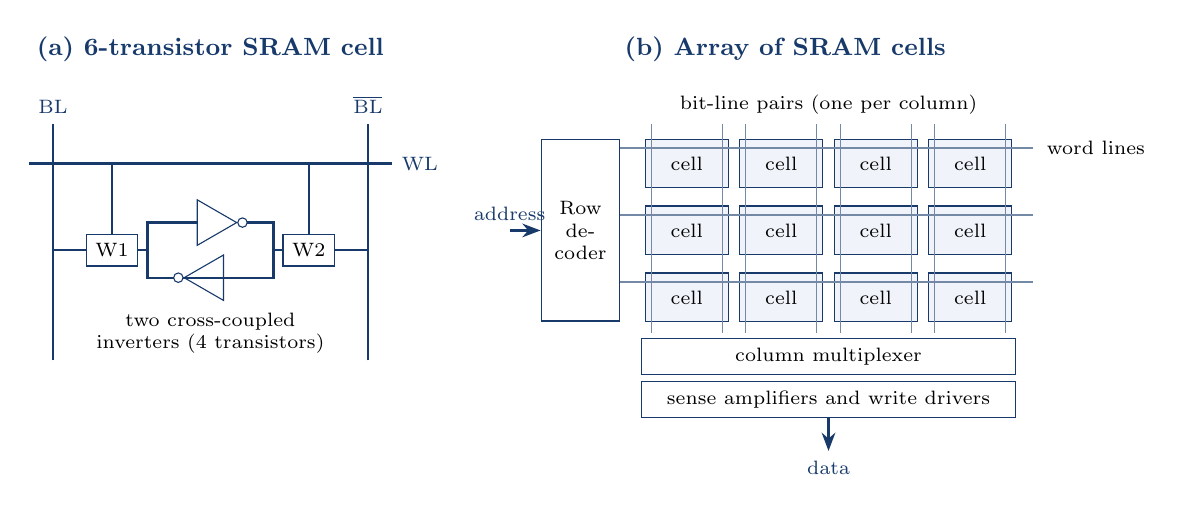
\begin{tikzpicture}[x=1cm,y=1cm,
  wire/.style={draftblue,thick},
  tr/.style={draw=draftblue,fill=white,minimum width=0.5cm,minimum height=0.36cm,font=\scriptsize},
  cell/.style={draw=draftblue,fill=draftlight,minimum width=1.05cm,minimum height=0.62cm,font=\scriptsize,align=center},
  blk/.style={draw=draftblue,fill=white,font=\scriptsize,align=center},
  lab/.style={font=\scriptsize}]
\begin{scope}
\draw[wire] (0,0) -- (0,3.0) node[above,lab]{BL};
\draw[wire] (4,0) -- (4,3.0) node[above,lab]{$\overline{\mathrm{BL}}$};
\draw[wire] (-0.3,2.5) -- (4.3,2.5) node[right,lab]{WL};
\node[tr] (w1) at (0.75,1.4) {W1};
\node[tr] (w2) at (3.25,1.4) {W2};
\draw[wire] (0,1.4) -- (w1.west); \draw[wire] (w2.east) -- (4,1.4);
\draw[wire] (0.75,2.5) -- (w1.north); \draw[wire] (3.25,2.5) -- (w2.north);
\node[draw=draftblue,fill=white,isosceles triangle,isosceles triangle apex angle=60,minimum size=0.5cm,inner sep=0pt] (i1) at (2,1.75) {};
\node[draw=draftblue,fill=white,isosceles triangle,isosceles triangle apex angle=60,minimum size=0.5cm,inner sep=0pt,shape border rotate=180] (i2) at (2,1.05) {};
\draw[draftblue,fill=white] (i1.apex) ++(0.06,0) circle (0.06);
\draw[draftblue,fill=white] (i2.apex) ++(-0.06,0) circle (0.06);
\draw[wire] (w1.east) -- (1.2,1.4);
\draw[wire] (1.2,1.4) |- (i1.west); \draw[wire] (1.2,1.4) |- ($(i2.apex)+(-0.12,0)$);
\draw[wire] (w2.west) -- (2.8,1.4);
\draw[wire] (2.8,1.4) |- ($(i1.apex)+(0.12,0)$); \draw[wire] (2.8,1.4) |- (i2.west);
\node[lab,align=center] at (2,0.35) {two cross-coupled\\inverters (4 transistors)};
\node[font=\small\bfseries,text=draftblue] at (2,3.95) {(a) 6-transistor SRAM cell};
\end{scope}
\begin{scope}[xshift=6.3cm]
\node[blk,minimum width=1.0cm,minimum height=2.3cm] (dec) at (0.4,1.65) {Row\\de-\\coder};
\foreach \r in {0,1,2}{
  \foreach \c in {0,1,2,3}{ \node[cell] at (1.75+\c*1.2,2.5-\r*0.85) {cell}; }
  \draw[wire,draftblue!60] (0.9,2.5-\r*0.85+0.2) -- (6.15,2.5-\r*0.85+0.2);}
\node[lab,anchor=west] at (6.2,2.7) {word lines};
\foreach \c in {0,1,2,3}{\draw[draftblue!60] (1.3+\c*1.2,3.0) -- (1.3+\c*1.2,0.35); \draw[draftblue!60] (2.2+\c*1.2,3.0) -- (2.2+\c*1.2,0.35);}
\node[blk,minimum width=4.75cm,minimum height=0.42cm] at (3.55,0.05) {column multiplexer};
\node[blk,minimum width=4.75cm,minimum height=0.42cm] at (3.55,-0.5) {sense amplifiers and write drivers};
\draw[-{Stealth},thick,draftblue] (-0.5,1.65) -- (dec.west) node[pos=0,above,lab]{address};
\draw[-{Stealth},thick,draftblue] (3.55,-0.72) -- (3.55,-1.15) node[below,lab]{data};
\node[lab] at (3.55,3.25) {bit-line pairs (one per column)};
\node[font=\small\bfseries,text=draftblue] at (3.0,3.95) {(b) Array of SRAM cells};
\end{scope}
\end{tikzpicture}
\caption[SRAM cell and array]{(a) A six-transistor SRAM cell: the word line (WL) turns on the access transistors W1 and W2, connecting the cross-coupled inverters to the complementary bit lines. (b) Cells are arranged in a two-dimensional array; a decoder raises one word line, every cell in that row drives its bit lines, and a column multiplexer and sense amplifiers select and read the bits required. Redrawn after Sarangi \cite[sec.~7.4.1, Figs.~7.26--7.27]{sarangi2025basic}.}
\label{fig:sram-array}
\end{figure}


Cell size sets the density gap between SRAM and DRAM. Using 2012-era figures, the textbook gives an SRAM cell an area of about 0.08\,\textmu m$^2$ and an array access time of 1--5 cycles, against about 0.005\,\textmu m$^2$ and 50--200 cycles for a DRAM cell \cite[sec.~11.1.1, Table~11.1]{sarangi2025basic}. SRAM is thus roughly sixteen times larger per bit but far faster, which is why it is used for on-chip caches and why a cache of tens of megabytes takes a large share of a die (\cref{sec:planar-limits}).

Main memory is built from DRAM instead (\cref{fig:dram-array}). A DRAM cell stores a bit as charge on a capacitor, reached through a single access transistor that the word line switches on, so it needs one transistor where SRAM needs six \cite[sec.~7.4.3]{sarangi2025basic}. The charge leaks away slowly, and reading the cell also drains some of it onto the bit line, so every cell must be rewritten after each read and refreshed periodically. A DRAM array therefore has a refresh circuit on its bit lines, a single bit line per column, and sense amplifiers placed before the column multiplexer, where they keep the whole open row (a DRAM \emph{page}) so that further accesses to that row are served quickly \cite[sec.~7.4.3]{sarangi2025basic}. The density is what makes DRAM suitable for large off-chip memories, and the extra steps are part of why it is so much slower.

\begin{figure}[htbp]
\centering
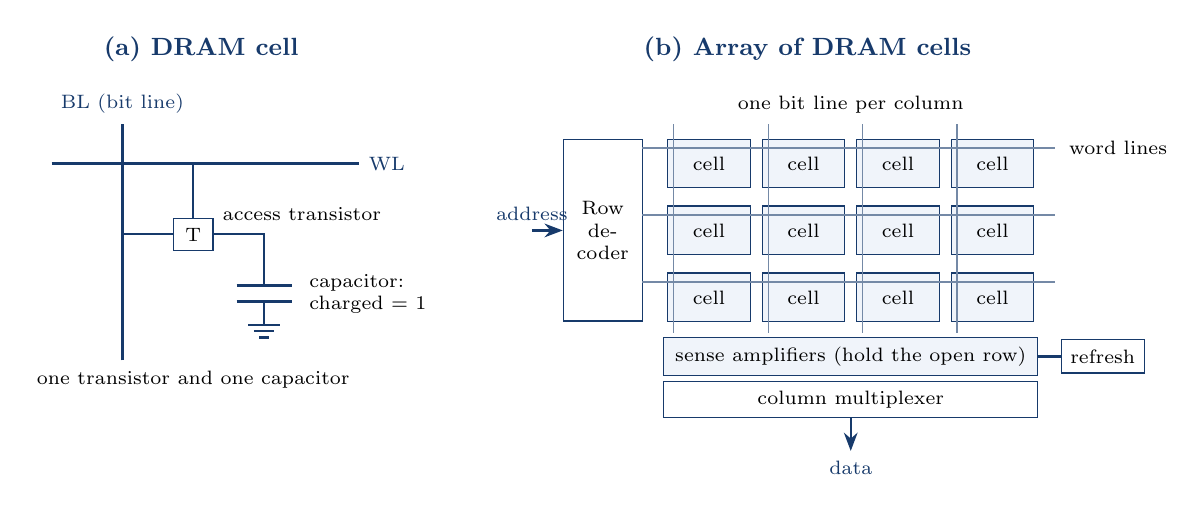
\begin{tikzpicture}[x=1cm,y=1cm,
  wire/.style={draftblue,thick},
  cell/.style={draw=draftblue,fill=draftlight,minimum width=1.05cm,minimum height=0.62cm,font=\scriptsize,align=center},
  blk/.style={draw=draftblue,fill=white,font=\scriptsize,align=center},
  lab/.style={font=\scriptsize}]
\begin{scope}
\draw[wire] (0.6,0) -- (0.6,3.0) node[above,lab]{BL (bit line)};
\draw[wire] (-0.3,2.5) -- (3.6,2.5) node[right,lab]{WL};
\node[draw=draftblue,fill=white,minimum width=0.5cm,minimum height=0.36cm,font=\scriptsize] (t) at (1.5,1.6) {T};
\draw[wire] (0.6,1.6) -- (t.west);
\draw[wire] (1.5,2.5) -- (t.north);
\draw[wire] (t.east) -- (2.4,1.6) -- (2.4,1.1);
\draw[wire] (2.4,1.1) -- (2.4,0.95);
\draw[draftblue,very thick] (2.05,0.95) -- (2.75,0.95);
\draw[draftblue,very thick] (2.05,0.75) -- (2.75,0.75);
\draw[wire] (2.4,0.75) -- (2.4,0.45);
\draw[wire] (2.2,0.45) -- (2.6,0.45); \draw[wire] (2.27,0.37) -- (2.53,0.37); \draw[wire] (2.34,0.29) -- (2.46,0.29);
\node[lab,anchor=west,align=left] at (2.85,0.85) {capacitor:\\charged = 1};
\node[lab,anchor=south west,align=left] at (1.75,1.65) {access transistor};
\node[lab,align=center] at (1.5,-0.25) {one transistor and one capacitor};
\node[font=\small\bfseries,text=draftblue] at (1.6,3.95) {(a) DRAM cell};
\end{scope}
\begin{scope}[xshift=6.3cm]
\node[blk,minimum width=1.0cm,minimum height=2.3cm] (dec) at (0.4,1.65) {Row\\de-\\coder};
\foreach \r in {0,1,2}{
  \foreach \c in {0,1,2,3}{ \node[cell] at (1.75+\c*1.2,2.5-\r*0.85) {cell}; }
  \draw[wire,draftblue!60] (0.9,2.5-\r*0.85+0.2) -- (6.15,2.5-\r*0.85+0.2);}
\node[lab,anchor=west] at (6.2,2.7) {word lines};
\foreach \c in {0,1,2,3}{\draw[draftblue!60] (1.3+\c*1.2,3.0) -- (1.3+\c*1.2,0.35);}
\node[blk,minimum width=4.75cm,minimum height=0.42cm,fill=draftlight] at (3.55,0.05) {sense amplifiers (hold the open row)};
\node[blk,minimum width=4.75cm,minimum height=0.42cm] at (3.55,-0.5) {column multiplexer};
\node[blk,minimum width=1.0cm,minimum height=0.42cm] (rf) at (6.75,0.05) {refresh};
\draw[thick,draftblue] (rf.west) -- (5.93,0.05);
\draw[-{Stealth},thick,draftblue] (-0.5,1.65) -- (dec.west) node[pos=0,above,lab]{address};
\draw[-{Stealth},thick,draftblue] (3.55,-0.72) -- (3.55,-1.15) node[below,lab]{data};
\node[lab] at (3.55,3.25) {one bit line per column};
\node[font=\small\bfseries,text=draftblue] at (3.0,3.95) {(b) Array of DRAM cells};
\end{scope}
\end{tikzpicture}
\caption[DRAM cell and array]{(a) A DRAM cell: one access transistor, switched by the word line, connects a capacitor to a single bit line; a charged capacitor stores a 1. (b) Compared with the SRAM array of \cref{fig:sram-array}, a DRAM array has one bit line per column instead of two, a refresh circuit that writes the data back after every read and periodically, and sense amplifiers placed before the column multiplexer, where they hold the whole open row so that further accesses to it are fast. Redrawn after Sarangi \cite[sec.~7.4.3, Figs.~7.30--7.31]{sarangi2025basic}.}
\label{fig:dram-array}
\end{figure}

\subsection{Average memory access time}
\label{sec:amat}

The average memory access time (\gls{amat}) of a hierarchy is defined recursively \cite[sec.~11.3.1]{sarangi2025basic}:\index{AMAT}
\begin{equation}
\begin{aligned}
  \mathrm{AMAT} &= t_1 + m_1 \times \mathrm{penalty}_1,\\
  \mathrm{penalty}_{k} &= t_{k+1} + m_{k+1} \times \mathrm{penalty}_{k+1},
\end{aligned}
\label{eq:amat}
\end{equation}
where $t_k$ is the hit time and $m_k$ the local miss rate of level $k$, and the penalty of the last cache level is the main-memory latency. Because the lower levels are weighted by the miss rates above them, a long memory latency adds little to the average. With the latencies measured on a Zen~2 and a Zen~3 desktop part \cite{justiceAMDRyzen72021} and illustrative local miss rates of 5, 30 and 40\% for L1, L2 and L3, the L3 and a 60--70\,ns memory together add only about half a nanosecond to an average access of about 1.5\,ns. Each load that does miss still stalls for the full latency, which an out-of-order core can only partly overlap.

\Cref{eq:amat} shows precisely what a larger last-level cache can and cannot do:
\begin{itemize}
  \item it can lower $m_{\mathrm{LLC}}$, so fewer accesses pay the main-memory latency;
  \item but if making the cache larger also lengthens its hit time $t_{\mathrm{LLC}}$, part of the gain is lost on every LLC hit.
\end{itemize}
The design problem for a large LLC is therefore to add capacity while keeping the added hit latency small. That is the problem 3D stacking attacks (Part~\ref{part:stacked-cache}).

\subsection{Classifying cache misses}
\label{sec:miss-classes}

The textbook divides misses into three classes \cite[sec.~11.3.2]{sarangi2025basic}:\index{cache miss}
\begin{itemize}
  \item \textbf{Compulsory (cold) misses} occur the first time a block is accessed.
  \item \textbf{Capacity misses} occur when the program's working set\index{working set}---the blocks it uses over a typical interval---is larger than the cache.
  \item \textbf{Conflict misses} occur in direct-mapped and set-associative caches when more blocks map to one set than the set can hold.
\end{itemize}
A larger LLC primarily removes capacity misses. It therefore helps workloads whose working set exceeds the original cache but fits in the larger one, and helps little when the working set either already fits or is far larger than either size. This simple argument predicts the strongly workload-dependent results examined in Part~\ref{part:case-study}.

\subsection{Cache organisation and policies}
\label{sec:cache-org}
A cache stores fixed-size \emph{blocks} (typically 32--128 bytes) and records which memory addresses it holds in a \emph{tag array} beside the \emph{data array}. An address is divided into a tag, an index and an offset within the block. In a \emph{fully associative} cache a block may be placed anywhere, so every tag must be compared on each access; this is practical only for small structures because of its area and power. A \emph{direct-mapped} cache allows each block exactly one location, selected by the index bits, which is simple and fast but suffers conflict misses. A \emph{set-associative}\index{set-associative cache} cache is the compromise used almost universally: the index selects a set of $K$ locations (the associativity, typically 2, 4 or 8 in the textbook's examples), and the tags of that set are compared in parallel \cite[sec.~11.2.2]{sarangi2025basic}. AMD's Zen~3 L3, for comparison, is 16-way set associative both with and without V-Cache \cite[slides~19--20]{wuu2022vcache}. \Cref{fig:set-assoc} shows the lookup.

\begin{figure}[htbp]
\centering
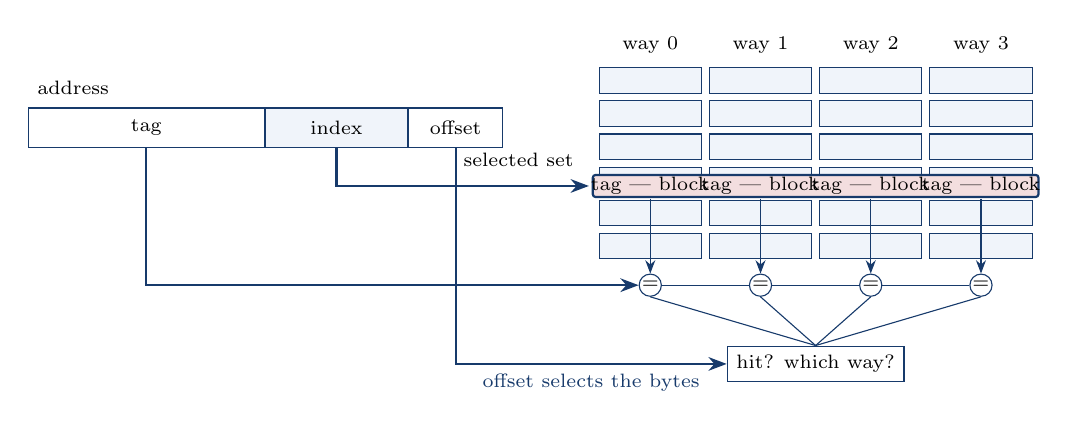
\begin{tikzpicture}[x=1cm,y=1cm,
  fld/.style={draw=draftblue,minimum height=0.5cm,font=\scriptsize,align=center},
  way/.style={draw=draftblue,fill=draftlight,minimum width=1.3cm,minimum height=0.32cm,font=\scriptsize},
  lab/.style={font=\scriptsize}]
\node[fld,minimum width=3.0cm,fill=white] (tag) at (0,0) {tag};
\node[fld,minimum width=1.8cm,fill=draftlight,right=0pt of tag] (idx) {index};
\node[fld,minimum width=1.2cm,fill=white,right=0pt of idx] (off) {offset};
\node[lab,above=1pt of tag.north west,anchor=south west] {address};
\foreach \s in {0,...,5}{
  \foreach \w in {0,1,2,3}{\node[way] at (6.4+\w*1.4,0.6-\s*0.42) {};}}
\foreach \w in {0,1,2,3}{\node[lab] at (6.4+\w*1.4,1.05) {way \w};}
\draw[draftblue,thick,rounded corners=1pt,fill=todored!15] (5.67,-0.88) rectangle (11.33,-0.6);
\foreach \w in {0,1,2,3}{\node[font=\scriptsize] at (6.4+\w*1.4,-0.74) {tag | block};}
\node[lab,anchor=south east] at (5.55,-0.62) {selected set};
\draw[-{Stealth},thick,draftblue] (idx.south) |- (5.62,-0.74);
\foreach \w in {0,1,2,3}{
  \node[draw=draftblue,circle,inner sep=0.5pt,font=\scriptsize,fill=white] (c\w) at (6.4+\w*1.4,-2.0) {$=$};
  \draw[-{Stealth},draftblue] (6.4+\w*1.4,-0.9) -- (c\w.north);}
\draw[-{Stealth},thick,draftblue] (tag.south) |- (6.0,-2.0) -- (c0.west);
\draw[draftblue] (c0.east) -- (c1.west) (c1.east) -- (c2.west) (c2.east) -- (c3.west);
\node[draw=draftblue,fill=white,font=\scriptsize,align=center] (hit) at (8.5,-3.0) {hit? which way?};
\foreach \w in {0,1,2,3}{\draw[draftblue] (c\w.south) -- (hit.north);}
\draw[-{Stealth},thick,draftblue] (off.south) |- (hit.west) node[pos=0.75,below,lab]{offset selects the bytes};
\end{tikzpicture}
\caption[Lookup in a 4-way set-associative cache]{Lookup in a 4-way set-associative cache. The index bits select one set; the tags stored in all four ways of that set are compared with the address tag in parallel; a match identifies the way holding the block, and the offset selects the bytes within it. After Sarangi \cite[sec.~11.2.2]{sarangi2025basic}.}
\label{fig:set-assoc}
\end{figure}

\textbf{Tags in a large cache.} The index and offset bits are fixed by the number of sets and the block size, so the tag takes the remaining address bits \cite[sec.~11.2.2]{sarangi2025basic}. With Zen~3's 64-byte lines and a 48-bit physical address \cite[p.~10]{advancedmicrodevicesinc.UsingSEVAMD2023}, the 16-way 32\,MB L3 \cite[slide~19]{wuu2022vcache} still stores a 27-bit tag per line, so tag storage grows almost in proportion to capacity (\cref{sec:cache-interface}). The 8-way 32\,KB L1 uses only the low 12 address bits for its index and offset, the offset within a 4\,KB page, which lets it be indexed while the address is being translated (\cref{sec:virtual-memory}).
\label{sec:address-example}

Organisation can also be matched to how a program walks through its data. Wang, for example, proposes an L1 cache for two-dimensional data, such as matrices and images, that stores data in a hierarchical Z-order layout across multiple banks so that either a square tile or a row can be read in one access. In matrix-multiplication simulations this reduced both L1 cache misses and misses in the translation lookaside buffer (TLB, \cref{sec:virtual-memory}) compared with a conventional row-by-row layout \cite{wangDesignImplementationCache2019}. The example is far from AMD's last-level cache, but it illustrates the same principle from the other direction: instead of adding capacity to hold a working set, it rearranges data so that the existing capacity is used better.

When a set is full, a \emph{replacement policy} chooses a victim: random replacement is simplest, FIFO evicts the oldest block, and least-recently-used (LRU), which follows directly from the stack-distance view of temporal locality, is among the most effective \cite[sec.~11.2.5]{sarangi2025basic}. Writes are handled either \emph{write-through}, sending every write to the next level, or \emph{write-back}\index{write-back cache}, marking a block as modified and writing it back only on eviction, which reduces traffic at the cost of tracking state \cite[sec.~11.2.3]{sarangi2025basic}. The stacked V-Cache keeps this organisation intact: each die's portion of the L3 has its own data, tag and LRU arrays \cite[slide~20]{wuu2022vcache}.

The textbook summarises the main cache optimisations and their side effects; \cref{tab:cache-optimisations} reproduces the entries most relevant to this paper. The table makes the paper's central tension explicit: the standard remedy for capacity misses is a larger cache, and its listed costs are higher latency, higher power and more area.

\begin{table}[htbp]
  \centering
  \caption[Selected memory-system optimisations and their costs, after Sarangi]{Selected memory-system optimisations and their costs, after Sarangi \cite[Table~11.2]{sarangi2025basic}.}
  \label{tab:cache-optimisations}
  \small
  \begin{tabularx}{\textwidth}{@{}>{\raggedright\arraybackslash}p{4.3cm}>{\raggedright\arraybackslash}p{4.2cm}>{\raggedright\arraybackslash}X@{}}
    \toprule
    \textbf{Technique} & \textbf{Targets} & \textbf{Disadvantages} \\
    \midrule
    Larger block size & compulsory misses & fewer blocks in the cache \\
    Prefetching & compulsory and capacity misses & complexity; may displace useful data \\
    \textbf{Larger cache} & \textbf{capacity misses} & \textbf{higher latency, higher power, more area} \\
    Higher associativity & conflict misses & higher latency, higher power \\
    Victim cache & conflict misses & extra complexity \\
    Small, simple cache & hit time & higher miss rate \\
    Write buffer, critical word first & miss penalty & extra complexity \\
    \bottomrule
  \end{tabularx}
\end{table}

\Cref{fig:mindmap-misses} arranges the same techniques around the terms of \cref{eq:amat} that they target.

\mapfigure{%
\node[mmroot] (r) {Lowering average memory access time};
\node[mmbox,mmlevel1,fill=mmCFE0F4] (b0) at (0.00,3.60) {Compulsory misses};
\draw[mmbig] (r) -- (b0);
\node[mmlevel2,mmbox,fill=mmF9D7AF] (b0c0) at (-1.52,5.35) {Larger blocks};
\draw[mmsmall] (b0.north) to[out=90,in=-90] (b0c0.south);
\node[mmlevel2,mmbox,fill=mmF9D7AF] (b0c1) at (1.52,5.35) {Prefetching};
\draw[mmsmall] (b0.north) to[out=90,in=-90] (b0c1.south);
\node[mmbox,mmlevel1,fill=mmF9D7AF] (b1) at (4.47,1.36) {Capacity misses};
\draw[mmbig] (r) -- (b1);
\node[mmlevel2,mmbox,fill=mmDCCFF6] (b1c0) at (8.07,2.08) {Larger cache: 3D V-Cache};
\draw[mmsmall] (b1.east) to[out=0,in=180] (b1c0.west);
\node[mmlevel2,mmoval,fill=mmDCCFF6] (b1c1) at (8.07,0.63) {Prefetching};
\draw[mmsmall] (b1.east) to[out=0,in=180] (b1c1.west);
\node[mmbox,mmlevel1,fill=mmCFE7E1] (b2) at (2.76,-3.56) {Conflict misses};
\draw[mmbig] (r) -- (b2);
\node[mmlevel2,mmbox,fill=mmF9D7AF] (b2c0) at (6.36,-2.83) {Higher associativity};
\draw[mmsmall] (b2.east) to[out=0,in=180] (b2c0.west);
\node[mmlevel2,mmbox,fill=mmF9D7AF] (b2c1) at (6.36,-4.28) {Victim cache};
\draw[mmsmall] (b2.east) to[out=0,in=180] (b2c1.west);
\node[mmbox,mmlevel1,fill=mmF4AAA2] (b3) at (-2.76,-3.56) {Hit time};
\draw[mmbig] (r) -- (b3);
\node[mmlevel2,mmbox,fill=mmCFE7E1] (b3c0) at (-6.36,-3.56) {Small, simple cache};
\draw[mmsmall] (b3.west) to[out=180,in=0] (b3c0.east);
\node[mmoval,mmlevel1,fill=mmDCCFF6] (b4) at (-4.47,1.36) {Miss penalty};
\draw[mmbig] (r) -- (b4);
\node[mmlevel2,mmbox,fill=mmF4C2BB] (b4c0) at (-8.07,2.08) {Write buffer};
\draw[mmsmall] (b4.west) to[out=180,in=0] (b4c0.east);
\node[mmlevel2,mmbox,fill=mmF4C2BB] (b4c1) at (-8.07,0.63) {Critical word first};
\draw[mmsmall] (b4.west) to[out=180,in=0] (b4c1.east);
}{[Overview of \cref{tab:cache-optimisations}]{Overview of \cref{tab:cache-optimisations}: the three miss classes and the AMAT terms, and the techniques that target each \cite[Table~11.2]{sarangi2025basic}. The stacked cache of Part~\ref{part:stacked-cache} is a way of making the cache larger, so it attacks capacity misses, and it pays the price the table lists for that technique: higher latency, power and area.}}{fig:mindmap-misses}


3D V-Cache can be read as an attempt to take the third row of \cref{tab:cache-optimisations} while avoiding most of its disadvantages: the area cost moves to a separate die, and the latency cost is held to four cycles (\cref{sec:vcache-access}).

\subsection{Writes and inclusion}
\label{sec:writes-inclusion}
Before a store can write, the whole block must be in the cache, so even a one-byte store first brings in the entire block. A write-back cache then updates only its own copy and writes the block down when it is evicted, so writes are cheap and evictions carry the traffic \cite[sec.~11.2.3]{sarangi2025basic}.

Write-back is the usual choice at the larger levels, because the more often a block is rewritten before eviction, the more traffic it saves. The same reasoning applies at the bottom of the hierarchy. In a chiplet processor, the memory controllers sit on the I/O die (\cref{sec:d2d}), so modified blocks written back from a compute die's L3 must cross the die-to-die link to reach memory. A larger L3 that keeps blocks longer before eviction can therefore reduce write traffic on that link as well as read misses.

Write buffers and critical-word-first fetching shorten the miss penalty rather than the miss rate, and complement a larger cache rather than replace it \cite[sec.~11.3.3]{sarangi2025basic}.

\subsubsection*{Inclusion}
A hierarchy is \emph{inclusive}\index{inclusion} if every level holds a subset of the blocks in the level below it, and \emph{exclusive} if it does not follow strict inclusion \cite[sec.~11.1.7, Definition~100]{sarangi2025basic}. The textbook calls inclusive caches the convention, because they are simpler to design and avoid some correctness problems in multiprocessors, but notes that some advanced processors (as of 2025) use exclusive caches where they benefit from more flexible data placement \cite[sec.~11.1.7]{sarangi2025basic}. Inclusion has a direct consequence for capacity. In an inclusive hierarchy the caches add no storage, since each holds only copies of data in the level below; the total size of the memory system is that of main memory \cite[sec.~11.3]{sarangi2025basic}. The same holds between caches: an inclusive L3 keeps a copy of every block in the L2s above it, so the number of distinct blocks a die holds on chip is set by the L3 alone. An exclusive L3 adds its capacity to that of the L2s. A second consequence follows from the definition. In an inclusive hierarchy, a block that is not in the shared level cannot be in any private cache above it, so one lookup in the shared level answers for the whole group of cores.

\Cref{tab:inclusion-example} applies this to a Zen~3 core complex (CCX), the group of cores that shares one L3, whose eight cores have up to 4\,MB of L2 between them and share a 32\,MB L3, or 96\,MB with 3D V-Cache \cite[sec.~2.2]{amd2022epyc7003}. The sources used in this paper do not state which inclusion policy Zen~3's L3 follows, so the table gives both cases.

\begin{table}[htbp]
  \centering
  \caption[Distinct on-chip capacity of one Zen~3 CCX under the two inclusion policies]{Distinct on-chip capacity of one Zen~3 CCX under the two inclusion policies (8 cores $\times$ 512\,KB L2 \cite[sec.~2.2]{amd2022epyc7003}).}
  \label{tab:inclusion-example}
  \small
  \begin{tabular}{@{}lccc@{}}
    \toprule
    \textbf{L3} & \textbf{Inclusive L3} & \textbf{Exclusive L3} & \textbf{Difference} \\
    \midrule
    32\,MB (planar) & 32\,MB & 36\,MB & 12.5\% \\
    96\,MB (V-Cache) & 96\,MB & 100\,MB & 4.2\% \\
    \midrule
    Ratio, V-Cache to planar & 3.0$\times$ & 2.8$\times$ & \\
    \bottomrule
  \end{tabular}
\end{table}

The policy matters less as the L3 grows. With the cache die, the L2s are a small fraction of the total, so V-Cache roughly triples the distinct capacity of a CCX under either policy. Comparisons that hold the policy fixed, as all the comparisons in Part~\ref{part:case-study} do because the plain and V-Cache parts share one core design, are not affected by it.

\subsection{Virtual memory and address translation}
\label{sec:virtual-memory}
Programs use \emph{virtual} addresses, which are translated page by page to \emph{physical} addresses through a per-process \emph{page table} \cite[sec.~11.4.3]{sarangi2025basic}. With 4\,KB pages, the low 12 bits of an address are the offset within the page and pass through translation unchanged; only the page number is replaced. Recent translations are cached in a small TLB\index{TLB}, and a TLB miss stalls the pipeline for the tens of cycles needed to read the page table \cite[sec.~11.4.3]{sarangi2025basic}.

\textbf{TLB reach.} The memory a TLB can translate without a miss, its \emph{reach}\index{TLB!reach}, is its number of entries times the page size. With 4\,KB pages, Zen~3's 64-entry first-level and 2048-entry second-level data TLBs \cite{7-cpu.comAMDZen3} reach 256\,KB and 8\,MB, a quarter of a 32\,MB L3 and a twelfth of a 96\,MB stacked L3; with 2\,MB pages the first level alone covers 128\,MB, more than either L3 (\cref{app:tlb-reach}). A program that touches a large working set at random with 4\,KB pages can therefore hit in the L3 and still miss in both TLBs. The group's measurement on a Ryzen~5 5600X agrees (\cref{app:5600x}): with 4\,KB pages latency starts to rise just above 256\,KB and again from about 7\,MB, and at 1\,GB address translation adds about 17\,ns to every access, a figure that the nested translation of the virtual machine (the Windows Subsystem for Linux, WSL2) probably inflates.

Three points follow for the rest of the paper. First, latency sweeps with 4\,KB pages measure cache and TLB effects together, which Part~\ref{part:case-study} has to allow for when it reads the steps in a latency curve (\cref{sec:milanx-latency}). Second, for a program using 4\,KB pages, the benefit of a larger L3 is the benefit to the whole memory system, including any translation cost the L3 does not remove. Third, the observation in \cref{sec:address-example} that the L1 index and offset use only the low 12 bits matters here: those bits are the page offset, which translation does not change, so the L1 lookup can start before the TLB has finished.

\subsection{Overlapping misses and multithreading}
\label{sec:mlp}
The textbook's memory-stall model, $\mathrm{CPI} = \mathrm{CPI}_{\mathrm{ideal}} + f_{\mathrm{mem}} \times (\mathrm{AMAT} - 1)$, where $f_{\mathrm{mem}}$ is the fraction of instructions that access memory, assumes that the pipeline stalls for every cycle of every access beyond the first \cite[sec.~11.3.1]{sarangi2025basic}. That is exact for the textbook's five-stage in-order pipeline, but it overstates the stall of an out-of-order core. Such a core keeps issuing independent instructions from its window while a load waits (\cref{sec:pipelining-power}), and those instructions can include other loads, so several misses can be outstanding at once. If $n$ independent misses are in flight together, the core waits about one memory latency for all of them, so each costs roughly $t_{\mathrm{mem}}/n$. This overlap is usually called \emph{memory-level parallelism}\index{memory-level parallelism}. A simple way to express it is a hidden fraction $h$ (the model of \cref{sec:sim-study} uses its complement, the exposed fraction $\omega = 1 - h$, which it calls the overlap factor):
\begin{equation}
  \text{stall cycles per thousand instructions} \;\approx\; \mathrm{MPKI} \times (1 - h) \times t_{\mathrm{mem}},
  \label{eq:mlp-stall}
\end{equation}
where MPKI is the number of misses to memory per thousand instructions and $t_{\mathrm{mem}}$ the memory latency in cycles. With $h = 0$ this is the textbook's model; with independent misses, $h$ rises towards $1 - 1/n$.

For the textbook's memory latency of 100--300 cycles \cite[sec.~12.4.8]{sarangi2025basic}, a core that keeps two independent misses in flight ($h = 0.5$) waits 50--150 cycles per miss, and one that keeps four ($h = 0.75$) waits 25--75. Removing a miss saves only what it would have cost, so these values bound what a larger cache can gain per removed miss; Part~\ref{part:stacked-cache} compares them with what a measurement implies (\cref{sec:tradeoff-example}).

A Zen~3 measurement shows the same effect directly for TLB misses. 7-cpu.com reports a first-level TLB miss penalty of 7 cycles when misses occur one at a time, but only 1.7 cycles per access when independent misses overlap; for the second-level TLB the figures are 24 and 5 cycles \cite{7-cpu.comAMDZen3}. The hardware thus overlaps the equivalent of about four to five TLB misses.

The overlap explains a pattern that recurs in Parts~\ref{part:stacked-cache} and~\ref{part:case-study}. A latency sweep walks a chain of pointers in which each load's address depends on the previous one, so no two misses can overlap and the sweep sees the full latency of every level: a nearly five-fold difference between Milan and Milan-X at 64\,MB (\cref{sec:milanx-latency}). Real programs usually have some independent misses, so removing a miss saves less, and whole-program gains are measured in per cent rather than multiples. Programs that chase pointers, such as graph traversals, are closer to the latency sweep and should gain more per removed miss; programs that stream through memory overlap their misses well and gain less.

A second way to hide memory latency is to give the pipeline other threads to run. The textbook describes three forms of \emph{multithreading} \cite[sec.~12.4.8]{sarangi2025basic}. A \emph{coarse-grained} multithreaded processor keeps the context of several threads in the pipeline and switches among them every $n$ cycles or on a long-latency event such as an L2 miss, so while one memory-intensive thread waits 100--300 cycles for memory, another can do useful work. \emph{Fine-grained} multithreading switches every one or two cycles. \emph{Simultaneous multithreading} (SMT), the form used in modern multiple-issue cores, shares the issue slots of each cycle dynamically among the threads, so a stall in one thread is filled with instructions from the others. The textbook lists its costs: a more complex fetch stage, harder coherence and consistency, and a higher memory-bandwidth requirement than an equivalent single-threaded core \cite[sec.~12.4.8]{sarangi2025basic}. The threads also split the core's resources between them \cite[sec.~12.4.8, Important Point~20]{sarangi2025basic}, including its caches.

Zen~3 supports SMT, so one CCX runs up to 16 hardware threads: each core's two threads share its 512\,KB L2, and all sixteen share the 32\,MB L3, or 96\,MB with V-Cache \cite[sec.~2.2]{amd2022epyc7003}. With every thread busy, that is $32/16 = 2$\,MB of L3 per thread on a planar CCD and $96/16 = 6$\,MB on a stacked one. SMT and a larger cache therefore interact. SMT hides latency but divides capacity and raises the demand for bandwidth; a larger L3 restores capacity per thread and removes some of the extra misses. Part~\ref{part:synthesis} returns to the bandwidth side of this interaction (\cref{sec:bandwidth-wall}).

\subsection{Beyond SRAM: alternative LLC technologies}
Stacking SRAM is not the only way to obtain a larger last-level cache. Denser technologies such as stacked DRAM \cite{mittalSurveyTechniquesArchitecting2016} and STT-RAM \cite{kimExploitingDataCompression2022} change the \emph{technology} of the cache, whereas AMD's 3D V-Cache keeps SRAM and changes its \emph{placement}; \cref{sec:llc-alternatives} compares them with the figures the sources report.

\section{Multicore Processors, Coherence and Interconnects}
\label{sec:multicore}

\subsection{From one core to many}
The textbook traces the move to multicore processors from the mid-2000s as transistor budgets continued to grow while single-core power and complexity limits tightened \cite[sec.~12.1]{sarangi2025basic}. Multicore processors raise two questions that matter directly for chiplets: how cores keep a consistent view of shared data, and how requests travel between cores, caches and memory.

\subsection{How far parallelism goes: Amdahl's law}
More cores help only to the extent that a program can use them. If a fraction $f_{\mathrm{seq}}$ of a program's running time is sequential and the rest divides perfectly among $P$ processors, the speedup is
\begin{equation}
  S \;=\; \frac{1}{f_{\mathrm{seq}} + (1 - f_{\mathrm{seq}})/P},
  \label{eq:amdahl}
\end{equation}
which approaches $1/f_{\mathrm{seq}}$ however many processors are added \cite[sec.~12.2.3]{sarangi2025basic}. With $f_{\mathrm{seq}} = 5\%$ the limit is 20, and the textbook notes that there is then no appreciable difference between 35 and 200 processors \cite[sec.~12.2.3]{sarangi2025basic}.

Amdahl's law has two consequences for this paper. First, a 64-core chiplet processor does not mainly serve one parallel program: its typical use is to run many unrelated programs or requests at once, which the textbook calls loosely coupled multiprocessing and which scales almost perfectly because the programs barely interact \cite[sec.~12.2.1]{sarangi2025basic}. That is the market the chiplet organisation serves. Second, for any single program the sequential part still runs on one core, so the performance of each core, set by its clock, its IPC and the cache it can reach, still decides the limit. Stacked cache improves exactly that per-core performance, which is why it complements adding cores.

\subsection{Cache coherence}
When several caches can hold copies of the same address, \gls{cache-coherence} rules ensure that all threads observe writes to that address in a consistent order \cite[sec.~12.4.2]{sarangi2025basic}. In a chiplet processor, a coherence transaction between cores on different compute dies must cross the die-to-die interconnect, so the physical partitioning becomes visible as latency (\cref{sec:d2d}).

A multicore memory system can use \emph{shared} caches, which every core accesses, or \emph{private} caches, each serving one core or a small group of cores. The textbook compares them directly (\cref{tab:shared-private}): private caches are small, fast and close to their cores but must be kept coherent and replicate shared data, while shared caches avoid replication and coherence traffic but are large, slow and far from most cores \cite[sec.~12.4.4]{sarangi2025basic}. Its conclusion is that the first levels should be private and the lower, larger levels shared.

\begin{table}[htbp]
  \centering
  \caption[Private versus shared caches, after Sarangi]{Private versus shared caches, after Sarangi \cite[Table~12.3]{sarangi2025basic}.}
  \label{tab:shared-private}
  \small
  \begin{tabular}{@{}lll@{}}
    \toprule
    \textbf{Attribute} & \textbf{Private cache} & \textbf{Shared cache} \\
    \midrule
    Area & low & high \\
    Speed & fast & slow \\
    Proximity to the processor & near & far \\
    Scalability in size & low & high \\
    Data replication & yes & no \\
    Complexity & high (needs coherence) & low \\
    \bottomrule
  \end{tabular}
\end{table}

A large shared cache is not built as one monolithic array. To serve many cores at once, it is split into \emph{banks}, each a smaller cache in its own right selected by some of the address bits; banking reduces contention and makes each bank faster and more power-efficient \cite[sec.~12.4.5]{sarangi2025basic}.

Private caches are made to look like one shared cache by a coherence protocol\index{cache coherence}. The textbook states the requirement as two axioms: \emph{completion}, every write must eventually complete, and \emph{order}, all threads must see the writes to one address in the same order \cite[sec.~12.4.2]{sarangi2025basic}.

In a \emph{snooping} protocol\index{snooping protocol} the caches share a bus and broadcast read misses, write misses and writes; each block is tracked in a small state machine with the states Modified, Shared and Invalid \cite[sec.~12.4.6]{sarangi2025basic}. Because the bus carries one message at a time, every cache sees the same order of messages, which satisfies the order axiom. The textbook develops two such protocols. In \emph{write-update}, every write is broadcast so that all copies are updated. In \emph{write-invalidate}, a cache that wants to write first invalidates all other copies; a block may then be shared by many readers or owned by a single writer, but never both, and writes to an owned block need no messages at all \cite[sec.~12.4.6]{sarangi2025basic}. \Cref{fig:msi-states} shows the write-invalidate state machine.

\begin{figure}[htbp]
\centering
\resizebox{\textwidth}{!}{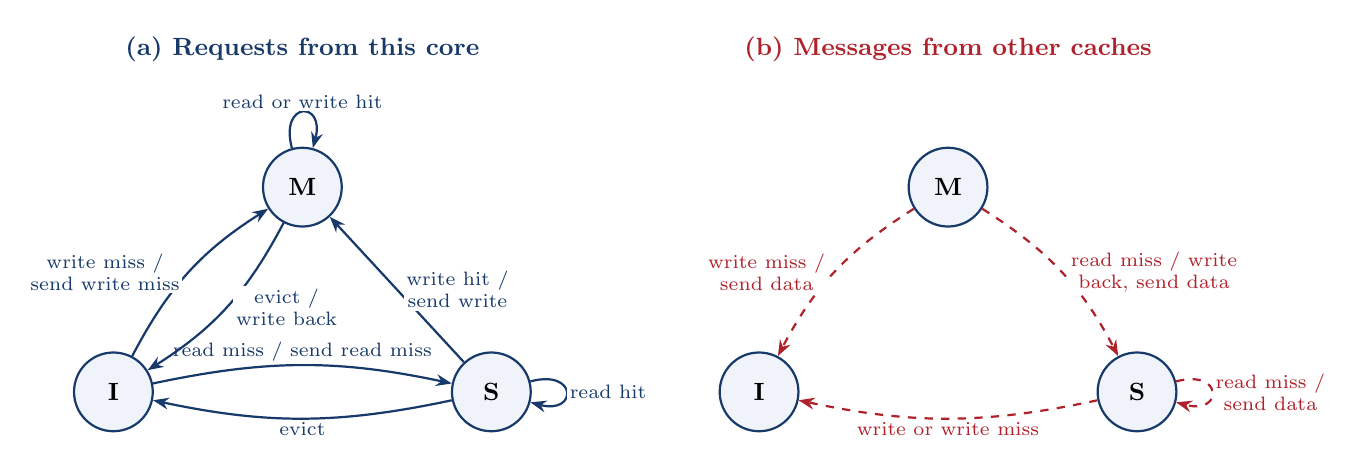
\begin{tikzpicture}[x=1cm,y=1cm,
  st/.style={circle,draw=draftblue,fill=draftlight,thick,minimum size=1.0cm,font=\small\bfseries},
  tr/.style={-{Stealth[length=2mm]},draftblue,thick},
  bt/.style={-{Stealth[length=2mm]},todored,thick,dashed},
  lab/.style={font=\scriptsize,align=center,fill=white,inner sep=1pt}]
\begin{scope}
\node[font=\small\bfseries,text=draftblue] at (2.4,4.35) {(a) Requests from this core};
\node[st] (I) at (0,0) {I};
\node[st] (S) at (4.8,0) {S};
\node[st] (M) at (2.4,2.6) {M};
\draw[tr] (I) to[bend left=12] node[lab,above]{read miss / send read miss} (S);
\draw[tr] (S) to[bend left=12] node[lab,below]{evict} (I);
\draw[tr] (I) to[bend left=15] node[lab,left=2pt]{write miss /\\send write miss} (M);
\draw[tr] (M) to[bend left=15] node[lab,right=2pt]{evict /\\write back} (I);
\draw[tr] (S) to node[lab,right=2pt]{write hit /\\send write} (M);
\draw[tr] (S) to[loop right,looseness=6] node[lab,right]{read hit} (S);
\draw[tr] (M) to[loop above,looseness=6] node[lab,above]{read or write hit} (M);
\end{scope}
\begin{scope}[xshift=8.2cm]
\node[font=\small\bfseries,text=todored] at (2.4,4.35) {(b) Messages from other caches};
\node[st] (I2) at (0,0) {I};
\node[st] (S2) at (4.8,0) {S};
\node[st] (M2) at (2.4,2.6) {M};
\draw[bt] (S2) to[bend left=12] node[lab,below]{write or write miss} (I2);
\draw[bt] (M2) to[bend right=15] node[lab,left=2pt]{write miss /\\send data} (I2);
\draw[bt] (M2) to[bend left=15] node[lab,right=2pt]{read miss / write\\back, send data} (S2);
\draw[bt] (S2) to[loop right,looseness=6] node[lab,right]{read miss /\\send data} (S2);
\end{scope}
\end{tikzpicture}}
\caption[The write-invalidate (MSI) snooping protocol]{The write-invalidate (MSI) snooping protocol for one cache block, redrawn after Sarangi \cite[sec.~12.4.6, Figs.~12.13--12.14]{sarangi2025basic}. (a) Transitions caused by this cache's own processor; (b) transitions caused by messages that other caches place on the bus. A block may be held by many caches in S, but by only one in M.}
\label{fig:msi-states}
\end{figure}

\Cref{tab:msi-example} traces a write-invalidate protocol through five accesses by two cores, A and B, to the same block, using the transitions of \cref{fig:msi-states}. Every step generates a bus message, and steps 2 and 4 also move the block's data between the caches.

\begin{table}[htbp]
  \centering
  \caption[Block states and bus traffic for two cores sharing one block]{Block states and bus traffic for two cores sharing one block (write-invalidate MSI).}
  \label{tab:msi-example}
  \small
  \begin{tabularx}{\textwidth}{@{}l>{\raggedright\arraybackslash}p{2.5cm}cc>{\raggedright\arraybackslash}X@{}}
    \toprule
    & \textbf{Access} & \textbf{A} & \textbf{B} & \textbf{Bus message and data movement} \\
    \midrule
    1 & A reads $x$ & I $\to$ S & I & read miss; data from the lower level \\
    2 & B reads $x$ & S & I $\to$ S & read miss; A or the lower level supplies the data \\
    3 & A writes $x$ & S $\to$ M & S $\to$ I & write; B invalidates its copy \\
    4 & B reads $x$ & M $\to$ S & I $\to$ S & read miss; A writes the block back and sends it to B \\
    5 & B writes $x$ & S $\to$ I & S $\to$ M & write; A invalidates its copy \\
    \bottomrule
  \end{tabularx}
\end{table}

On a chiplet processor, every message and every data transfer in the table must travel between the two caches. If A and B are on the same Zen CCD, the transfer stays on the die; if they are on different CCDs, each one crosses the die-to-die links through the I/O die (\cref{sec:d2d}). A block that is written alternately by two cores also ping-pongs between them, so the cost of the hop is paid repeatedly. Software that places communicating threads on the same CCD avoids this, which is one reason EPYC processors expose their CCD structure to the operating system (\cref{sec:d2d}). Broadcasting does not scale, so larger systems use a \emph{directory}\index{directory protocol} that records, for each block, which caches hold a copy, and sends messages only to those sharers \cite[sec.~12.4.6]{sarangi2025basic}.

The textbook's directory keeps the sharers as a bit vector with one bit per cache \cite[sec.~12.4.6]{sarangi2025basic}, which adds $N/512$ to every tracked 64-byte block for $N$ caches (12.5\% for 64); coherence tracking therefore grows harder as more caches, and more dies, share one memory. AMD's implementation is not described in the sources used here.

\textbf{What a directory buys.} \Cref{app:directory-example} repeats the five accesses of \cref{tab:msi-example} with a directory instead of a bus, under counting assumptions of the authors' own. The directory sends 18 messages whatever the number of caches, because only two caches ever hold the block, whereas a bus delivers each of the five steps to every other cache: $5(N-1)$ deliveries, 35 for eight caches and 315 for 64. The price is indirection: each step after the first passes through the directory and takes two sequential round trips instead of one bus transaction. A directory therefore trades latency for bandwidth, which is the right trade when there are many caches and few of them share any one block.

In a chiplet processor the indirection has a physical cost. If the requester, the directory and the owner sat on different dies, each arrow in \cref{tab:directory-example} (\cref{app:directory-example}) would cross a die-to-die link, and a four-message step would take two link round trips. The sources used here do not say where AMD keeps its coherence directory, so this is a statement about the textbook scheme. It is still a useful bound: \cref{sec:d2d} gives the cost of one such round trip on Rome, and Part~\ref{part:chiplets} returns to what coherence across dies costs in practice.

AMD's Zen designs combine both ideas at different scales. Within a Zen~3 CCD, eight cores share one L3; across CCDs, each L3 is private to its die, and the dies communicate through the I/O die over Infinity Fabric \cite{amd2022epyc7003}. EPYC~7003 can even expose each CCD's L3 as a separate non-uniform memory access (NUMA) domain to software \cite{amd2022epyc7003}. The textbook's trade-off therefore reappears one level up: the per-CCD L3 is ``private'' with respect to the whole socket, which keeps it close and fast but means that data shared across CCDs must be kept coherent over a die-to-die link (\cref{sec:d2d}).

\subsection{On-chip and on-package interconnection networks}
On a single die, cores, cache banks and memory controllers are usually arranged as tiles, each with a \emph{router}; the routers and the links between them form a network-on-chip (NoC) that carries coherence messages, LLC requests and responses, and memory traffic \cite[sec.~12.6.1]{sarangi2025basic}. Two figures of merit describe a topology: the \emph{bisection bandwidth}, the minimum number of links that must be cut to split the network into two equal halves, which measures both reliability and aggregate bandwidth; and the \emph{diameter}, the longest of all shortest paths between nodes, which bounds latency \cite[sec.~12.6.2]{sarangi2025basic}. \Cref{tab:topologies} lists the textbook's values.

\begin{table}[htbp]
  \centering
  \caption[Diameter and bisection bandwidth of common topologies]{Diameter and bisection bandwidth of common topologies with $N$ nodes, from Sarangi \cite[sec.~12.6.3]{sarangi2025basic}, with values for $N = 8$ (the CCDs of a Rome or Milan package, or the cores of a Zen~3 CCD) and $N = 64$ (the cores of the full processor).}
  \label{tab:topologies}
  \small
  \begin{tabular}{@{}lcccccc@{}}
    \toprule
    & \multicolumn{2}{c}{\textbf{Formula}} & \multicolumn{2}{c}{$N = 8$} & \multicolumn{2}{c}{$N = 64$} \\
    \cmidrule(lr){2-3}\cmidrule(lr){4-5}\cmidrule(l){6-7}
    \textbf{Topology} & \textbf{Diameter} & \textbf{Bisection} & \textbf{Diam.} & \textbf{Bisec.} & \textbf{Diam.} & \textbf{Bisec.} \\
    \midrule
    Chain & $N-1$ & 1 & 7 & 1 & 63 & 1 \\
    Ring & $N/2$ & 2 & 4 & 2 & 32 & 2 \\
    Fat tree & $2\log N$ & $N/2$ & 6 & 4 & 12 & 32 \\
    Mesh & $2\sqrt{N}-2$ & $\sqrt{N}$ & --- & --- & 14 & 8 \\
    Torus & $\sqrt{N}$ & $2\sqrt{N}$ & --- & --- & 8 & 16 \\
    Hypercube & $\log N$ & $N/2$ & 3 & 4 & 6 & 32 \\
    Butterfly & $\log N + 1$ & $N/2$ & 4 & 4 & 7 & 32 \\
    \bottomrule
  \end{tabular}
\end{table}

At eight nodes the ring is perfectly adequate: no node is more than four hops away. At 64 nodes the same ring would put cores up to 32 hops apart with a bisection of only 2, which is why large monolithic processors use meshes. AMD's chiplet designs avoid the problem by never building a 64-node network on one die. Within each CCD, a ring connects the eight cores to the L3 slices \cite{lamAMDs7950X3DZen2023}; across the package, the CCDs form a star around the I/O die, in which any two CCDs are two links apart (\cref{fig:topologies}). Chips and Cheese attributes AMD's L3 latency, 24--28 cycles lower on average than that of Intel's mesh-based server processors in its tests, to this choice: a ring has lower latency and higher bandwidth, while a mesh scales better for a large monolithic die \cite{cozmaDeepDivingZen2022}. The cost of the star is that its hub carries all traffic between dies, which is the bandwidth limit examined in \cref{sec:bandwidth-example}.

\begin{figure}[htbp]
\centering
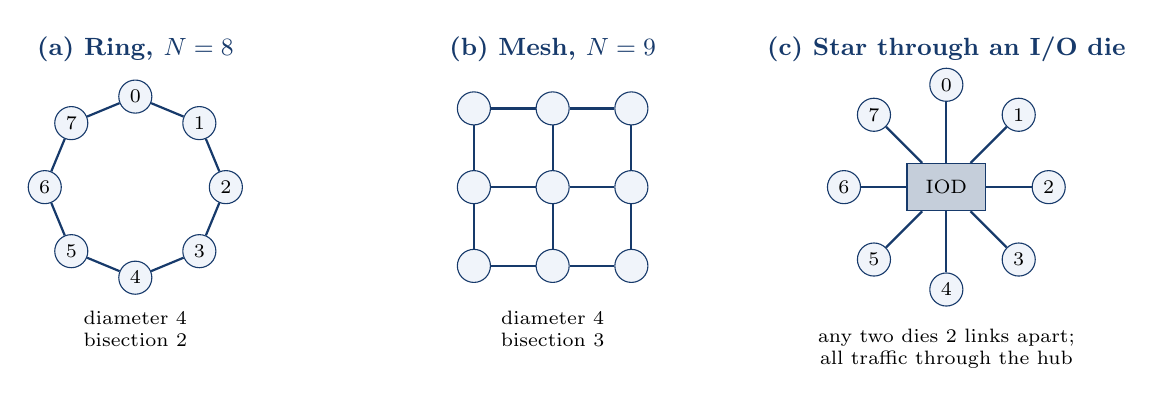
\begin{tikzpicture}[x=1cm,y=1cm,
  nd/.style={circle,draw=draftblue,fill=draftlight,minimum size=0.42cm,inner sep=0pt,font=\scriptsize},
  hub/.style={rectangle,draw=draftblue,fill=draftblue!25,minimum width=1.0cm,minimum height=0.6cm,font=\scriptsize},
  ln/.style={draftblue,thick},
  ttl/.style={font=\small\bfseries,text=draftblue}]
\begin{scope}
\node[ttl] at (0,1.75) {(a) Ring, $N=8$};
\foreach \i in {0,...,7}{\node[nd] (r\i) at ({90-45*\i}:1.15) {\i};}
\foreach \i in {0,...,7}{\pgfmathtruncatemacro\j{mod(\i+1,8)}\draw[ln] (r\i) -- (r\j);}
\node[font=\scriptsize,align=center] at (0,-1.8) {diameter 4\\bisection 2};
\end{scope}
\begin{scope}[xshift=4.3cm,yshift=-1.0cm]
\node[ttl] at (1.0,2.75) {(b) Mesh, $N=9$};
\foreach \x in {0,1,2}{\foreach \y in {0,1,2}{\node[nd] (m\x\y) at (\x,\y) {};}}
\foreach \x in {0,1,2}{\draw[ln] (m\x0) -- (m\x1) -- (m\x2); \draw[ln] (m0\x) -- (m1\x) -- (m2\x);}
\node[font=\scriptsize,align=center] at (1.0,-0.8) {diameter 4\\bisection 3};
\end{scope}
\begin{scope}[xshift=10.3cm]
\node[ttl] at (0,1.75) {(c) Star through an I/O die};
\node[hub] (h) at (0,0) {IOD};
\foreach \i in {0,...,7}{\node[nd] (s\i) at ({90-45*\i}:1.3) {\i}; \draw[ln] (h) -- (s\i);}
\node[font=\scriptsize,align=center] at (0,-2.05) {any two dies 2 links apart;\\all traffic through the hub};
\end{scope}
\end{tikzpicture}
\caption[Three topologies]{Three topologies. The ring and mesh follow Sarangi's definitions \cite[sec.~12.6.3]{sarangi2025basic}; the star is the arrangement of Rome's eight CCDs around one I/O die (\cref{sec:ccd-iod}). Within a CCD, Zen~3 and Zen~4 connect cores to L3 slices by a ring \cite{cozmaDeepDivingZen2022,lamAMDs7950X3DZen2023}.}
\label{fig:topologies}
\end{figure}

What changes when a link leaves the die is the subject of Part~\ref{part:chiplets}. On a die, a link is a set of short on-chip wires; between chiplets, it is a serialised link routed through the package, with its own transmitters, receivers and clocking. AMD's Rome processors connect every CCD to a single central I/O die, a star-like arrangement, which AMD credits with reducing the number of NUMA domains and the distances to memory compared with the previous generation \cite{naffziger2020chiplet}.
\clearpage
\part{Chiplet-Based Processor Architecture}
\label{part:chiplets}
\Cref{fig:mindmap-chiplets} maps the topics of this part.

\mapfigure{%
\node[mmroot] (r) {Chiplet-based processors};
\node[mmbox,mmlevel1,fill=mmF4AAA2] (b0) at (0.00,3.60) {Why split the die};
\draw[mmbig] (r) -- (b0);
\node[mmlevel2,mmbox,fill=mmCFE7E1] (b0c0) at (-3.05,5.35) {Yield falls with area};
\draw[mmsmall] (b0.north) to[out=90,in=-90] (b0c0.south);
\node[mmlevel2,mmbox,fill=mmCFE7E1] (b0c1) at (0.00,5.35) {Reticle limit};
\draw[mmsmall] (b0.north) to[out=90,in=-90] (b0c1.south);
\node[mmlevel2,mmbox,fill=mmCFE7E1] (b0c2) at (3.05,5.35) {I/O gains little from 7\,nm};
\draw[mmsmall] (b0.north) to[out=90,in=-90] (b0c2.south);
\node[mmbox,mmlevel1,fill=mmCFE7E1] (b1) at (4.07,2.20) {Who does what};
\draw[mmbig] (r) -- (b1);
\node[mmlevel2,mmbox,fill=mmF9D7AF] (b1c0) at (7.67,3.65) {CCD: cores, L2, L3};
\draw[mmsmall] (b1.east) to[out=0,in=180] (b1c0.west);
\node[mmlevel2,mmbox,fill=mmF9D7AF] (b1c1) at (7.67,2.20) {IOD: memory, PCIe, fabric};
\draw[mmsmall] (b1.east) to[out=0,in=180] (b1c1.west);
\node[mmlevel2,mmbox,fill=mmF9D7AF] (b1c2) at (7.67,0.75) {Same CCD, many products};
\draw[mmsmall] (b1.east) to[out=0,in=180] (b1c2.west);
\node[mmbox,mmlevel1,fill=mmCFE0F4] (b2) at (4.07,-2.20) {Die-to-die link};
\draw[mmbig] (r) -- (b2);
\node[mmlevel2,mmbox,fill=mmF9D7AF] (b2c0) at (7.67,-0.75) {AMD: round trip under 9\,ns};
\draw[mmsmall] (b2.east) to[out=0,in=180] (b2c0.west);
\node[mmlevel2,mmbox,fill=mmF9D7AF] (b2c1) at (7.67,-2.20) {About 55\,GB/s per link};
\draw[mmsmall] (b2.east) to[out=0,in=180] (b2c1.west);
\node[mmlevel2,mmbox,fill=mmF9D7AF] (b2c2) at (7.67,-3.65) {Energy per bit};
\draw[mmsmall] (b2.east) to[out=0,in=180] (b2c2.west);
\node[mmbox,mmlevel1,fill=mmF9D7AF] (b3) at (0.00,-3.60) {Packaging};
\draw[mmbig] (r) -- (b3);
\node[mmlevel2,mmbox,fill=mmDCCFF6] (b3c0) at (-3.05,-5.35) {Organic: $<150$\,\textmu m};
\draw[mmsmall] (b3.south) to[out=-90,in=90] (b3c0.north);
\node[mmlevel2,mmoval,fill=mmDCCFF6] (b3c1) at (0.00,-5.35) {2.5D: $<40$\,\textmu m};
\draw[mmsmall] (b3.south) to[out=-90,in=90] (b3c1.north);
\node[mmlevel2,mmoval,fill=mmDCCFF6] (b3c2) at (3.05,-5.35) {3D: $<9$\,\textmu m};
\draw[mmsmall] (b3.south) to[out=-90,in=90] (b3c2.north);
\node[mmoval,mmlevel1,fill=mmDCCFF6] (b4) at (-4.07,-2.20) {What software sees};
\draw[mmbig] (r) -- (b4);
\node[mmlevel2,mmbox,fill=mmF4C2BB] (b4c0) at (-7.67,-0.75) {NUMA distances};
\draw[mmsmall] (b4.west) to[out=180,in=0] (b4c0.east);
\node[mmlevel2,mmbox,fill=mmF4C2BB] (b4c1) at (-7.67,-2.20) {NPS1, 2, 4};
\draw[mmsmall] (b4.west) to[out=180,in=0] (b4c1.east);
\node[mmlevel2,mmbox,fill=mmF4C2BB] (b4c2) at (-7.67,-3.65) {LLC as NUMA};
\draw[mmsmall] (b4.west) to[out=180,in=0] (b4c2.east);
\node[mmbox,mmlevel1,fill=mmD6EBC6] (b5) at (-4.07,2.20) {Cost and checks};
\draw[mmbig] (r) -- (b5);
\node[mmlevel2,mmoval,fill=mmDCCFF6] (b5c0) at (-7.67,3.65) {Good dies per wafer};
\draw[mmsmall] (b5.west) to[out=180,in=0] (b5c0.east);
\node[mmlevel2,mmbox,fill=mmDCCFF6] (b5c1) at (-7.67,2.20) {One die: about 2$\times$ cost (AMD)};
\draw[mmsmall] (b5.west) to[out=180,in=0] (b5c1.east);
\node[mmlevel2,mmoval,fill=mmDCCFF6] (b5c2) at (-7.67,0.75) {Same core, one die};
\draw[mmsmall] (b5.west) to[out=180,in=0] (b5c2.east);
}{[Overview of Part~\ref{part:chiplets}]{Overview of Part~\ref{part:chiplets}. The figures are those discussed in the text: link latency and bandwidth for Rome (\cref{sec:d2d}), interconnect pitches from AMD's packaging talk (\cref{tab:packaging-levels}), AMD's cost estimate (\cref{fig:chiplet-cost-chart}) and the Cezanne comparison (\cref{sec:cezanne}).}}{fig:mindmap-chiplets}

\section{Why Large Monolithic Dies Become Costly}
\label{sec:monolithic-limits}

\subsection{The reticle limit and die size}
A single die cannot be larger than the area a lithography tool can expose in one field. AMD's Hot Chips~33 presentation plots server CPU and GPU die sizes growing towards this reticle limit over roughly the last fifteen years \cite{swaminathanAdvancedPackagingEnabling2021}. For its second-generation EPYC (``Rome'') processor, AMD states that the 64-core top configuration would not be practical as a monolithic chip and would lie well beyond the maximum reticle size \cite{naffziger2020chiplet}.\index{reticle limit} The numbers show by how much (\cref{fig:reticle-sizes}). AMD's chart of die sizes draws the reticle limit at about 800\,mm$^2$ (read from the chart) \cite[slide~3]{swaminathanAdvancedPackagingEnabling2021}. Rome's eight 74\,mm$^2$ CCDs and its 416\,mm$^2$ I/O die add up to 1008\,mm$^2$ \cite{naffziger2020chiplet}, the ``about 1000\,mm$^2$'' AMD quotes \cite[slide~19]{suggs2019zen2}. Built as one die with the same areas, the 64-core part would therefore be about a quarter larger than the reticle allows, and even its compute alone, $8 \times 74 = 592$\,mm$^2$, would be about three quarters of the limit.

\begin{figure}[htbp]
\centering
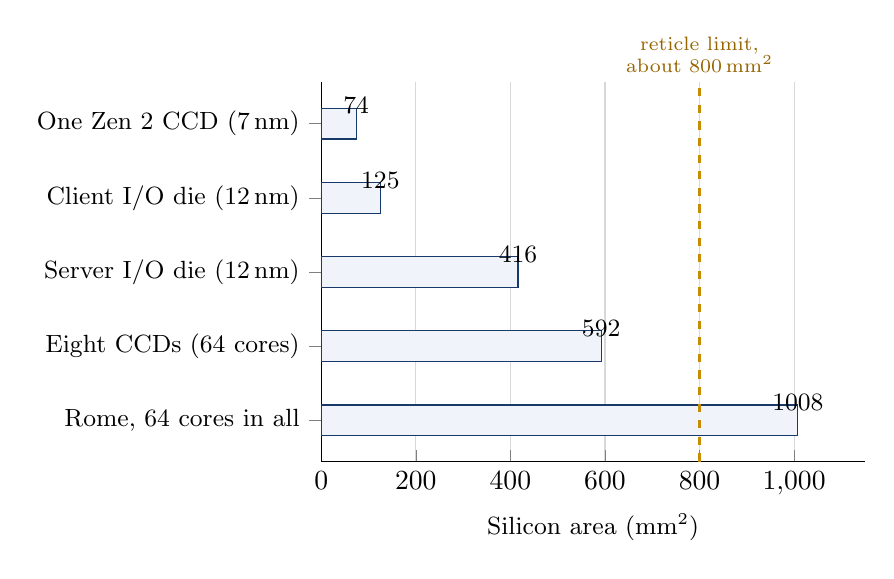
\begin{tikzpicture}
\begin{axis}[
  xbar, bar width=11pt, width=0.7\textwidth, height=6.4cm,
  xmin=0, xmax=1150, xlabel={Silicon area (mm$^2$)}, xlabel style={font=\small},
  symbolic y coords={ccd,client,server,eight,rome}, ytick=data, y dir=reverse,
  yticklabels={{One Zen~2 CCD (7\,nm)},{Client I/O die (12\,nm)},{Server I/O die (12\,nm)},{Eight CCDs (64 cores)},{Rome, 64 cores in all}},
  yticklabel style={font=\small, align=right},
  nodes near coords, nodes near coords style={font=\small}, point meta=explicit symbolic,
  xmajorgrids, grid style={draftgray!25}, axis x line*=bottom, axis y line*=left, enlarge y limits=0.14,
  clip=false]
\addplot[fill=draftlight,draw=draftblue] coordinates {(74,ccd)[74] (125,client)[125] (416,server)[416] (592,eight)[592] (1008,rome)[1008]};
\draw[very thick, dashed, color={rgb,255:red,200;green,140;blue,0}] ({axis cs:800,ccd} |- {rel axis cs:0,0}) -- ({axis cs:800,ccd} |- {rel axis cs:0,1});
\node[font=\scriptsize, color={rgb,255:red,150;green,100;blue,0}, anchor=south, align=center] at ({axis cs:800,ccd} |- {rel axis cs:0,1}) {reticle limit,\\about 800\,mm$^2$};
\end{axis}
\end{tikzpicture}
\caption[The 64-core Rome against the reticle limit]{The 64-core Rome against the reticle limit. Die areas are AMD's \cite{naffziger2020chiplet}; together they make the ``about 1000\,mm$^2$'' AMD gives for Rome \cite[slide~19]{suggs2019zen2}. The reticle limit is the line drawn in AMD's chart of server CPU and GPU die sizes \cite[slide~3]{swaminathanAdvancedPackagingEnabling2021}, read from its logarithmic axis as about 800\,mm$^2$ (approximate). A single die holding all of Rome would exceed it by about a quarter, and even the eight CCDs' 592\,mm$^2$ of compute alone would be a very large die.}
\label{fig:reticle-sizes}
\end{figure}

\subsection{Manufacturing yield}
\label{sec:yield-cost}

Manufacturing defects are scattered across a wafer, so a larger die is more likely to contain one. The simplest model assumes that defects fall independently with a fixed average density $D_0$, which gives a Poisson yield $e^{-AD_0}$ for a die of area $A$. Real defect densities vary across a wafer and from wafer to wafer, and the Poisson model ignores this. This paper therefore uses the yield model adopted in the 3D-IC cost analysis of Dong and Xie \cite[Eq.~15]{dongSystemlevelCostAnalysis2009}:
\begin{equation}
  Y_{\mathrm{die}} = Y_{\mathrm{wafer}} \cdot \frac{1 - e^{-2 A D_0}}{2 A D_0},
  \label{eq:yield}
\end{equation}
where $A$ is the die area, $D_0$ the average \gls{defect-density} and $Y_{\mathrm{wafer}}$ the wafer yield. This is one of the yield functions derived by Murphy, who averaged the Poisson yield over a defect density that varies from chip to chip; this form assumes the density is spread uniformly between $0$ and $2D_0$ \cite[Eq.~11]{murphyCostsizeOptimaMonolithic1964}. \Cref{app:yield-cost} derives it and compares it with Murphy's preferred intermediate model.\index{yield}\index{Murphy yield model}

\Cref{tab:yield-example} gives an illustrative calculation with $D_0 = 0.2$ defects/cm$^2$ and $Y_{\mathrm{wafer}} = 1$. It is a model result, not a measured processor result.

\begin{table}[htbp]
  \centering
  \caption[Illustrative Murphy-model yield]{Illustrative Murphy-model yield for $D_0 = 0.2$ defects/cm$^2$ and $Y_{\mathrm{wafer}} = 1$.}
  \label{tab:yield-example}
  \begin{tabular}{@{}lcc@{}}
    \toprule
    \textbf{Die area} & \textbf{$2 A D_0$} & \textbf{Modelled yield $Y_{\mathrm{die}}$} \\
    \midrule
    100 mm$^2$ (1 cm$^2$) & 0.4 & 82.4\% \\
    200 mm$^2$ (2 cm$^2$) & 0.8 & 68.8\% \\
    \bottomrule
  \end{tabular}
\end{table}

Doubling the die area lowers the modelled yield from about 82.4\% to 68.8\% (\cref{fig:yield-curve}). Cost per good die rises faster than area for two reasons: fewer dies fit on each wafer, and a smaller fraction of them work. The exact increase depends on wafer cost, process node, defect distribution and test cost; \cref{app:yield-cost} derives the cost-per-good-die expression and shows why partitioning a design into smaller dies can lower the silicon cost even after paying for extra interface area.

\begin{figure}[htbp]
\centering
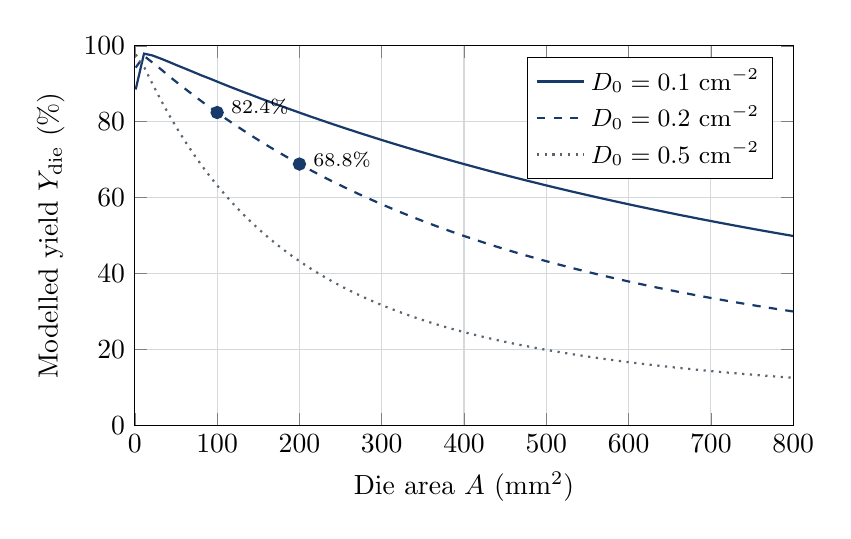
\begin{tikzpicture}
\begin{axis}[
  width=0.82\textwidth, height=6.4cm,
  xlabel={Die area $A$ (mm$^2$)}, ylabel={Modelled yield $Y_{\mathrm{die}}$ (\%)},
  xmin=0, xmax=800, ymin=0, ymax=100, grid=major, grid style={draftgray!25},
  legend pos=north east, legend style={font=\small},
  every axis plot/.append style={thick,domain=1:800,samples=80}]
\addplot[draftblue] {100*(1-exp(-2*x/100*0.1))/(2*x/100*0.1)}; \addlegendentry{$D_0=0.1$ cm$^{-2}$}
\addplot[draftblue,dashed] {100*(1-exp(-2*x/100*0.2))/(2*x/100*0.2)}; \addlegendentry{$D_0=0.2$ cm$^{-2}$}
\addplot[draftgray,dotted] {100*(1-exp(-2*x/100*0.5))/(2*x/100*0.5)}; \addlegendentry{$D_0=0.5$ cm$^{-2}$}
\addplot[only marks,mark=*,draftblue,mark size=2pt] coordinates {(100,82.42) (200,68.83)};
\node[font=\scriptsize,anchor=west] at (axis cs:105,84) {82.4\%};
\node[font=\scriptsize,anchor=west] at (axis cs:205,70) {68.8\%};
\end{axis}
\end{tikzpicture}
\caption[Murphy yield model for three illustrative defect densities]{Murphy yield model (\cref{eq:yield}, $Y_{\mathrm{wafer}}=1$) for three illustrative defect densities. The marked points reproduce the calculation in \cref{sec:yield-cost}. Illustrative calculation, not measured processor data.}
\label{fig:yield-curve}
\end{figure}

AMD's own material makes the same qualitative point. Its Zen~2 presentation lists ``small die improve yield'' among the motivations for the chiplet strategy \cite{suggs2019zen2}, and its Hot Chips~33 presentation shows normalised cost per yielded square millimetre rising at each newer process node \cite{swaminathanAdvancedPackagingEnabling2021}.

\subsection{Uneven scaling of logic, SRAM and analog circuits}
\label{sec:uneven-scaling}
Moving a design to a newer node does not shrink every circuit equally. Naffziger \emph{et al.} state that shrink factors at advanced nodes are much lower for analog circuitry than for digital logic and SRAM, and that memory interfaces and SerDes therefore gain very little performance, power or area from moving from 12\,nm to 7\,nm \cite{naffziger2020chiplet}. Building those circuits on the expensive leading-edge node wastes its cost. This observation is the basis of process-node specialisation (\cref{sec:process-specialisation}).

AMD's own charts show the trend (\cref{fig:area-scaling}). Logic and SRAM shrink together down to 10\,nm, after which SRAM falls behind, while analog and I/O circuits hardly shrink at all after 16\,nm \cite[slide~6]{wuu2022vcache}. At the same time the cost of each yielded square millimetre rises: read from AMD's chart, it is about 2.2 times the 45\,nm cost at 14\,nm, 3.7 times at 7\,nm and 4.9 times at 5\,nm. A circuit that does not shrink on the new node therefore costs several times as much per function there as on an older one.

\begin{figure}[htbp]
\centering
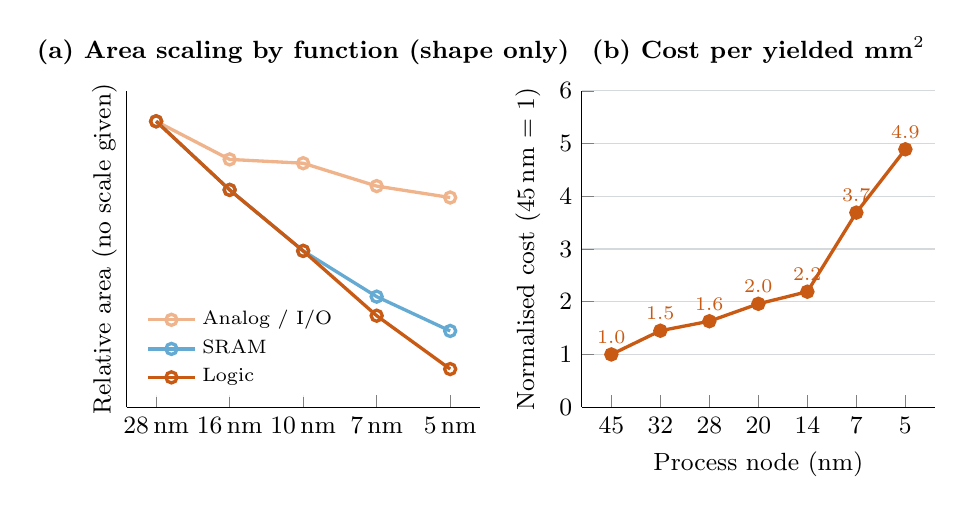
\begin{tikzpicture}
\begin{axis}[
  name=a, width=0.5\textwidth, height=5.6cm,
  title={\small\bfseries (a) Area scaling by function (shape only)},
  symbolic x coords={28nm,16nm,10nm,7nm,5nm}, xtick=data,
  xticklabels={28\,nm,16\,nm,10\,nm,7\,nm,5\,nm}, xticklabel style={font=\small},
  ymin=0.25, ymax=1.08, yticklabels={}, ytick=\empty,
  ylabel={Relative area (no scale given)}, ylabel style={font=\small},
  axis x line*=bottom, axis y line*=left,
  legend style={font=\scriptsize, at={(0.03,0.03)}, anchor=south west, draw=none, fill=white, fill opacity=0.85, text opacity=1},
  legend cell align=left]
\addplot[very thick, color={rgb,255:red,240;green,180;blue,140}, mark=o] coordinates {(28nm,1) (16nm,0.90) (10nm,0.89) (7nm,0.83) (5nm,0.80)};
\addlegendentry{Analog / I/O}
\addplot[very thick, color={rgb,255:red,100;green,170;blue,210}, mark=o] coordinates {(28nm,1) (16nm,0.82) (10nm,0.66) (7nm,0.54) (5nm,0.45)};
\addlegendentry{SRAM}
\addplot[very thick, color={rgb,255:red,200;green,90;blue,20}, mark=o] coordinates {(28nm,1) (16nm,0.82) (10nm,0.66) (7nm,0.49) (5nm,0.35)};
\addlegendentry{Logic}
\end{axis}
\begin{axis}[
  at={(a.east)}, anchor=west, xshift=1.3cm, width=0.5\textwidth, height=5.6cm,
  title={\small\bfseries (b) Cost per yielded mm$^2$},
  symbolic x coords={45nm,32nm,28nm,20nm,14nm,7nm,5nm}, xtick=data,
  xticklabels={45,32,28,20,14,7,5}, xticklabel style={font=\small}, xlabel={Process node (nm)}, xlabel style={font=\small},
  ymin=0, ymax=6, ytick={0,1,...,6}, yticklabel style={font=\small},
  ylabel={Normalised cost (45\,nm = 1)}, ylabel style={font=\small},
  ymajorgrids, grid style={draftgray!25}, axis x line*=bottom, axis y line*=left,
  nodes near coords, nodes near coords style={font=\scriptsize, above}, point meta=explicit symbolic]
\addplot[very thick, color={rgb,255:red,200;green,90;blue,20}, mark=*] coordinates {(45nm,1.0)[1.0] (32nm,1.45)[1.5] (28nm,1.63)[1.6] (20nm,1.96)[2.0] (14nm,2.19)[2.2] (7nm,3.69)[3.7] (5nm,4.89)[4.9]};
\end{axis}
\end{tikzpicture}
\caption[Area scaling by circuit type and cost per yielded mm$^2$ (AMD)]{Why SRAM and analog circuits no longer shrink with logic, and why each newer node costs more. Both panels are redrawn from AMD's ISSCC~2022 presentation \cite[slide~6]{wuu2022vcache}; AMD's 2025 packaging talk shows the same curves \cite[slide~3]{lambertHeterogenousIntegrationHigh2025}. (a)~AMD's chart has no values on its area axis, so only the shape is reproduced, normalised to 28\,nm: logic and SRAM shrink together to 10\,nm, SRAM then falls behind, and analog and I/O circuits hardly shrink after 16\,nm. (b)~Cost per yielded mm$^2$ for a 250\,mm$^2$ die, read from AMD's chart (about $\pm 0.1$): about 2.2 times the 45\,nm cost at 14\,nm and almost 5 times at 5\,nm.}
\label{fig:area-scaling}
\end{figure}

\textbf{Where the Zen~2 gains came from.} AMD's Zen~2 presentation splits the doubling of instructions per unit of energy over the previous generation into three factors: 1.15$\times$ from higher IPC, 1.17$\times$ from design improvements and 1.47$\times$ from the 7\,nm process \cite[slide~4]{suggs2019zen2}. Multiplied together, $1.15 \times 1.17 \times 1.47 \approx 1.98$, which is AMD's ``2$\times$''. The process contributed the largest single share, but only to the circuits that shrink with it. Logic and SRAM in the cores benefit; memory interfaces and SerDes, by Naffziger \emph{et al.}'s account, barely do \cite{naffziger2020chiplet}. The chiplet split therefore places the 7\,nm process exactly where its 1.47$\times$ applies and spends the cheaper process everywhere else. The related, more recent observation that SRAM is falling behind logic is taken up in \cref{sec:why-cache-capacity}.

\section{Compute Dies, I/O Dies and Core Complexes}
\label{sec:ccd-iod}

\begin{figure}[htbp]
\centering
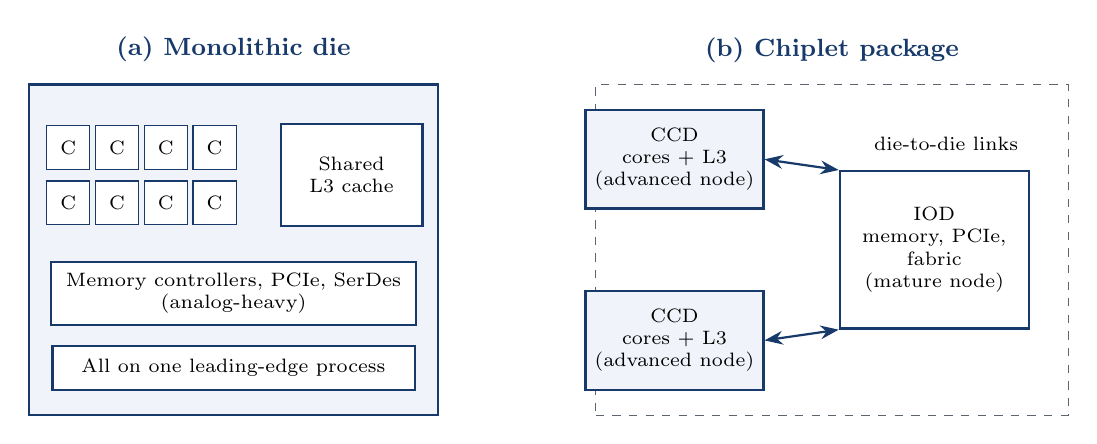
\begin{tikzpicture}[
  die/.style={draw=draftblue,thick,fill=draftlight,align=center,font=\scriptsize},
  core/.style={draw=draftblue,fill=white,minimum width=0.55cm,minimum height=0.55cm,font=\scriptsize},
  lab/.style={font=\small\bfseries,text=draftblue}]
\node[die,minimum width=5.2cm,minimum height=4.2cm] (mono) at (0,0) {};
\foreach \i in {0,...,3}{\foreach \j in {0,1}{
  \node[core] at (-2.1+\i*0.62,1.3-\j*0.7) {C};}}
\node[die,fill=white,minimum width=1.8cm,minimum height=1.3cm] at (1.5,0.95) {Shared\\L3 cache};
\node[die,fill=white,minimum width=4.6cm,text width=4.4cm,minimum height=0.8cm] at (0,-0.55) {Memory controllers, PCIe, SerDes\\(analog-heavy)};
\node[die,fill=white,minimum width=4.6cm,minimum height=0.55cm] at (0,-1.5) {All on one leading-edge process};
\node[lab,above=0.15cm of mono] {(a) Monolithic die};
\begin{scope}[xshift=7.6cm]
\node[draw=draftgray,dashed,minimum width=6.0cm,minimum height=4.2cm] (pkg) at (0,0) {};
\node[die,minimum width=1.5cm,minimum height=1.25cm] (c1) at (-2.0,1.15) {CCD\\cores + L3\\(advanced node)};
\node[die,minimum width=1.5cm,minimum height=1.25cm] (c2) at (-2.0,-1.15) {CCD\\cores + L3\\(advanced node)};
\node[die,minimum width=2.4cm,minimum height=2.0cm,fill=white] (iod) at (1.3,0) {IOD\\memory, PCIe,\\fabric\\(mature node)};
\draw[thick,draftblue,{Stealth}-{Stealth}] (c1.east) -- (iod.north west);
\node[font=\scriptsize,anchor=south] at ($(iod.north)+(0.15,0.12)$) {die-to-die links};
\draw[thick,draftblue,{Stealth}-{Stealth}] (c2.east) -- (iod.south west);
\node[lab,above=0.15cm of pkg] {(b) Chiplet package};
\end{scope}
\end{tikzpicture}
\caption[A monolithic die against a chiplet package]{Schematic contrast between a monolithic processor die and a chiplet package with compute dies (CCDs) and an I/O die (IOD). Illustrative only; not to scale and not an actual AMD floorplan.}
\label{fig:monolithic-vs-chiplet}
\end{figure}

AMD's Zen~2 products (``Rome'' for servers and ``Matisse'' for desktops) are built from three kinds of die \cite{naffziger2020chiplet,suggs2019zen2}:
\begin{itemize}
  \item an eight-core \gls{ccd}\index{CCD (core complex die)}\index{chiplet} of about 74\,mm$^2$ on a 7\,nm process, containing the cores and their L3 cache;
  \item a server \gls{iod}\index{I/O die (IOD)} of about 416\,mm$^2$ on a 12\,nm process;
  \item a smaller client IOD of about 125\,mm$^2$, which, packaged on its own, is also the X570 chipset.
\end{itemize}
The same CCD is reused across server and desktop products; only the IOD and the number of populated CCDs change \cite{naffziger2020chiplet}. Within each Zen~2 CCD, the cores are grouped into two four-core \glspl{ccx}\index{CCX (core complex)}, each with up to 16\,MB of L3 \cite{suggs2019zen2}. Inside a CCX, each core has a private 512\,KB L2, and the 16\,MB L3 is built from four 4\,MB slices, one beside each core, with 32-byte-per-cycle paths throughout; the CCX doubled both the L3 capacity and the L1 load/store bandwidth of the first Zen generation \cite[slide~12]{suggs2019zen2}.

AMD stated the problem and the response in two lists \cite[slide~13]{suggs2019zen2}. The challenges were a higher cost per mm$^2$ at the leading-edge node, analog and I/O circuits that ``do not scale well'' and are hard to port to a new process, and a wide range of markets to serve. The chiplet strategy answered each in turn: small dies to improve yield, analog and I/O on 12\,nm to reduce cost and complexity, and a configurable set of parts.

Of Rome's 1008\,mm$^2$ of silicon (\cref{fig:reticle-sizes}), 592\,mm$^2$ (59\%) is on the expensive 7\,nm process and 416\,mm$^2$ (41\%) on the cheaper 12\,nm \cite{naffziger2020chiplet}.

The partition places latency-critical, logic-dense circuits---cores and caches---on the newest node, and places memory controllers, PCI Express (PCIe) links and other I/O, which scale poorly, on a cheaper mature node (\cref{fig:monolithic-vs-chiplet}).

Naffziger \emph{et al.} describe how this partition was turned into products \cite{naffziger2020chiplet}. The server package places up to eight CCDs around a central IOD, in two-deep columns that were only possible because the organic-package link reaches farther than a silicon interposer would. Each CCD-to-IOD link is routed to the centre of the CCD to shorten the path to its L3. Not every server model populates all eight CCDs, so one package design yields a range of products. The desktop part reuses the same CCDs with a smaller IOD in the existing AM4 socket, and that IOD, packaged on its own, doubles as the platform's chipset. The previous server generation (``Naples'') tied its interface clocks together, whereas Rome decouples the fabric, memory and I/O clocks so that each can be set independently, with a latency-optimised mode when fabric and memory clocks are equal \cite{naffziger2020chiplet}. \Cref{fig:epyc-package} sketches the resulting server package.

\begin{figure}[htbp]
\centering
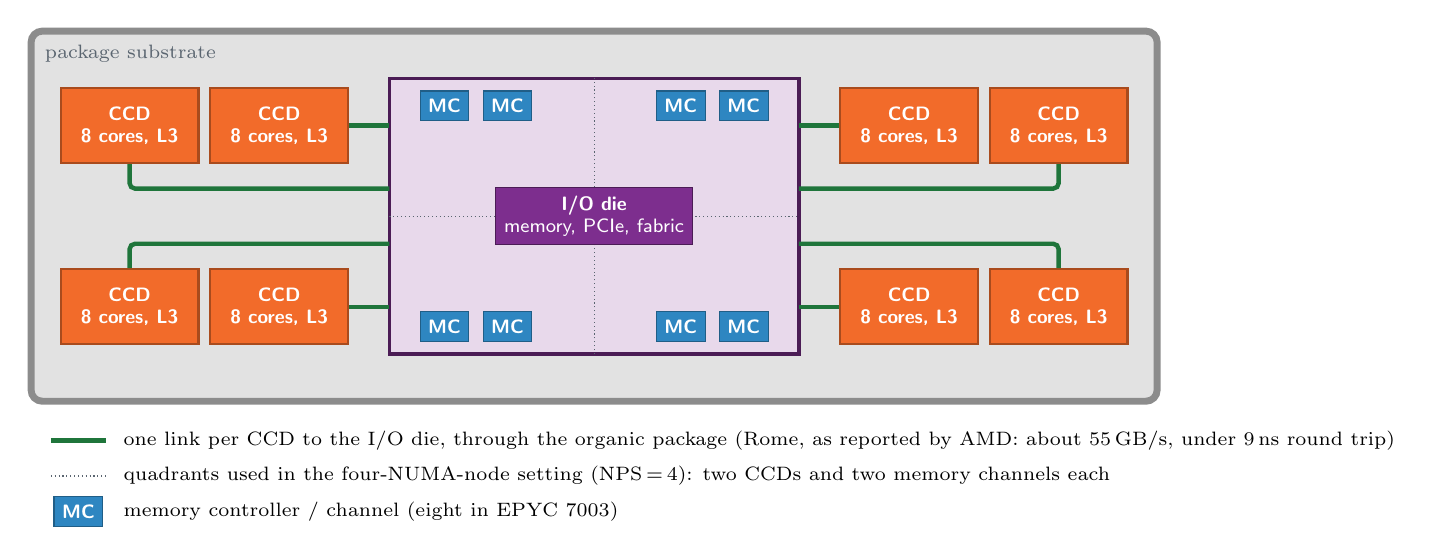
\begin{tikzpicture}[x=1cm,y=1cm,
  ccd/.style={draw=ccdcore!70!black,thick,fill=ccdcore,text=white,minimum width=1.75cm,minimum height=0.95cm,font=\sffamily\scriptsize\bfseries,align=center,inner sep=1pt},
  mc/.style={draw=ccdl2!70!black,fill=ccdl2,text=white,minimum width=0.62cm,minimum height=0.38cm,font=\sffamily\scriptsize\bfseries,inner sep=0pt},
  lnk/.style={ccdif!80!black,line width=1.6pt,rounded corners=2pt},
  lbl/.style={font=\scriptsize,align=left}]
\draw[ccdframe,line width=2.5pt,fill=ccdframe!25,rounded corners=4pt] (-7.15,-2.35) rectangle (7.15,2.35);
\node[font=\scriptsize,text=draftgray,anchor=north west] at (-7.1,2.3) {package substrate};
\draw[ccdl3!60!black,very thick,fill=ccdl3!18] (-2.6,-1.75) rectangle (2.6,1.75);
\draw[draftgray,densely dotted] (0,-1.75) -- (0,1.75) (-2.6,0) -- (2.6,0);
\foreach \x in {-1.9,-1.1,1.1,1.9}{\node[mc] at (\x,1.4) {MC}; \node[mc] at (\x,-1.4) {MC};}
\node[draw=ccdl3!60!black,fill=ccdl3,text=white,align=center,inner sep=3pt,font=\sffamily\scriptsize] at (0,0) {\textbf{I/O die}\\memory, PCIe, fabric};
\node[ccd] (LIU) at (-4.0, 1.15) {CCD\\8 cores, L3};
\node[ccd] (LOU) at (-5.9, 1.15) {CCD\\8 cores, L3};
\node[ccd] (LID) at (-4.0,-1.15) {CCD\\8 cores, L3};
\node[ccd] (LOD) at (-5.9,-1.15) {CCD\\8 cores, L3};
\node[ccd] (RIU) at ( 4.0, 1.15) {CCD\\8 cores, L3};
\node[ccd] (ROU) at ( 5.9, 1.15) {CCD\\8 cores, L3};
\node[ccd] (RID) at ( 4.0,-1.15) {CCD\\8 cores, L3};
\node[ccd] (ROD) at ( 5.9,-1.15) {CCD\\8 cores, L3};
\draw[lnk] (LIU.east) -- (-2.6, 1.15);  \draw[lnk] (LID.east) -- (-2.6,-1.15);
\draw[lnk] (LOU.south) |- (-2.6, 0.35); \draw[lnk] (LOD.north) |- (-2.6,-0.35);
\draw[lnk] (RIU.west) -- ( 2.6, 1.15);  \draw[lnk] (RID.west) -- ( 2.6,-1.15);
\draw[lnk] (ROU.south) |- ( 2.6, 0.35); \draw[lnk] (ROD.north) |- ( 2.6,-0.35);
\draw[lnk] (-6.9,-2.85) -- (-6.2,-2.85);
\node[lbl,anchor=west] at (-6.1,-2.85) {one link per CCD to the I/O die, through the organic package (Rome, as reported by AMD: about 55\,GB/s, under 9\,ns round trip)};
\draw[draftgray,densely dotted] (-6.9,-3.3) -- (-6.2,-3.3);
\node[lbl,anchor=west] at (-6.1,-3.3) {quadrants used in the four-NUMA-node setting (NPS\,=\,4): two CCDs and two memory channels each};
\node[mc] at (-6.55,-3.75) {MC};
\node[lbl,anchor=west] at (-6.1,-3.75) {memory controller / channel (eight in EPYC~7003)};
\end{tikzpicture}
\caption[Schematic of an AMD EPYC 7002/7003-style package]{Schematic of an AMD EPYC 7002/7003-style package: eight CCDs in two-deep columns around a central I/O die, each with its own link to the I/O die \cite{naffziger2020chiplet,amd2022epyc7003}. Positions, link routes and memory-controller placement are illustrative, not an actual AMD floorplan.}
\label{fig:epyc-package}
\end{figure}

\subsection{Inside the I/O die: memory, I/O and NUMA settings}
\label{sec:iod-detail}
AMD's EPYC~7003 overview describes what the I/O die of the Zen~3 server generation contains and how software sees it \cite{amd2022epyc7003}. Each CCD connects to the IOD through its own Global Memory Interconnect (GMI) link. The IOD holds eight Unified Memory Controllers, one per DDR4 channel, each supporting up to two memory modules (DIMMs), for up to 4\,TB of memory per socket; eight x16 I/O links that provide up to 128 lanes of PCIe~4.0; and the Infinity Fabric links that join the dies. The fabric clock can run at up to 1600\,MHz, which lets it run in step with DDR4-3200 memory, whose memory clock is also 1600\,MHz, a pairing AMD says improves memory latency \cite{amd2022epyc7003}. The IOD can be used with four, six or eight populated memory channels; eight is the most common and generally fastest configuration, and the six-channel option, with its own interleave mode, is new in this generation \cite{amd2022epyc7003}. AMD's figure labels this IOD as 14\,nm \cite[Fig.~2-4]{amd2022epyc7003}, while Naffziger \emph{et al.} give 12\,nm for the Rome IOD \cite{naffziger2020chiplet}; the sources used here do not resolve the difference.

\textbf{NUMA settings.}\index{NUMA} Because a core's distance to each memory controller depends on where both sit on the IOD, EPYC is a non-uniform memory access (NUMA) design, and a BIOS setting called NUMA Nodes Per Socket (NPS) lets the user choose how that structure is presented to software \cite{amd2022epyc7003}. The setting also decides how memory addresses are spread, or \emph{interleaved}, across channels: consecutive blocks of memory go to different channels in turn, so that a stream of accesses uses several channels at once. \Cref{tab:nps-modes} summarises the options.

\begin{table}[htbp]
  \centering
  \caption[NUMA settings of an EPYC~7003 processor]{NUMA settings of an EPYC~7003 processor with eight CCDs and eight memory channels, from AMD's description \cite{amd2022epyc7003}, with peak interleaved bandwidth worked out for DDR4-3200 ($25.6$\,GB/s per channel).}
  \label{tab:nps-modes}
  \small
  \begin{tabularx}{\textwidth}{@{}l>{\raggedright\arraybackslash}X>{\centering\arraybackslash}p{1.6cm}>{\centering\arraybackslash}p{2.4cm}@{}}
    \toprule
    \textbf{Setting} & \textbf{Each NUMA domain contains} & \textbf{Channels interleaved} & \textbf{Peak bandwidth per domain} \\
    \midrule
    NPS1 & the whole socket: all 8 CCDs, all channels, all PCIe devices & 8 & 204.8\,GB/s \\
    NPS2 & half the socket: 4 CCDs and 4 channels & 4 & 102.4\,GB/s \\
    NPS4 & one quadrant: 2 CCDs, 2 channels and 1 I/O hub & 2 & 51.2\,GB/s \\
    LLC as NUMA & one CCD and its L3 (8 domains per socket) & --- & --- \\
    \bottomrule
  \end{tabularx}
\end{table}
\textbf{What the setting trades.} In every NPS mode the socket's total memory bandwidth is the same, $8 \times 25.6 = 204.8$\,GB/s, and so is the share per core when all 64 cores are busy, $204.8/64 = 3.2$\,GB/s (\cref{tab:bandwidth-balance}). What changes is locality and reach. Under NPS4, a thread whose memory is allocated in its own quadrant reaches the nearest two controllers, the shortest core-to-memory distance on the die, but its interleaved accesses can draw on at most 51.2\,GB/s. Under NPS1, the same thread's accesses are spread over all eight channels and can draw on the full 204.8\,GB/s, but on average three quarters of them go to controllers outside its own quadrant, including the diagonal quadrant that AMD identifies as the farthest \cite{amd2022epyc7003}. NPS4 therefore suits many independent, well-placed workloads, and NPS1 suits a single program that needs bandwidth more than latency. The ``LLC as NUMA'' option goes one step further and tells the operating system which cores share an L3, so that threads that share data can be kept on one CCD and avoid the cross-die coherence traffic of \cref{sec:multicore} \cite{amd2022epyc7003}. The chiplet structure is thus exposed to software as a tuning choice: none of these settings would exist on a single die with uniform access to its memory controllers.

\section{Infinity Fabric and Die-to-Die Communication}
\label{sec:d2d}

Splitting a processor into dies turns some on-chip wires into package-level links. AMD connects each CCD to the IOD with an \gls{ifop} serial link routed over 10--20\,mm of organic package \cite{naffziger2020chiplet}. AMD reports, for Rome \cite{naffziger2020chiplet}:\index{Infinity Fabric}
\begin{itemize}
  \item about 55\,GB/s of effective bandwidth per IFOP link at a 1.46\,GHz fabric clock;
  \item a round-trip latency from CCD to IOD and back of 13 fabric clocks, under 9\,ns;
  \item longer reach than a 2.5D silicon interposer, which allowed two-deep columns of chiplets and hence eight CCDs in one package;
  \item a 19\% average reduction in memory latency for the socket compared with the previous generation, attributed to the central IOD, decoupled clocks and the latency-optimised link.
\end{itemize}
The predecessor ``Zeppelin'' link achieved about 2\,pJ/bit \cite{naffziger2020chiplet}. These are AMD-reported figures for specific configurations and are not independent measurements.

The link is engineered for low latency and power rather than maximum reach. Each IFOP lane runs at 14.6\,GT/s with a 1.46\,GHz fabric clock. It uses single-ended signalling to save power and package routing layers, forwards a clock alongside each bundle of data lanes to track skew, recovers each lane's timing with a digitally controlled clock-and-data-recovery circuit, and avoids active equalisation in favour of passive T-coils, again to save power \cite{naffziger2020chiplet}. The package itself had to be designed with the dies: the Rome package uses a 9-2-9 layer build-up (four signal-routing layers above the core) against 5-2-5 for Matisse. The dense arrays of package vias must lie outside the footprints of the CCDs and IOD because of the high density of power vias beneath them \cite{naffziger2020chiplet}. These are the costs of a serial, package-level link that the 3D interface of \cref{sec:cache-interface} avoids.

\subsection{Latency, bandwidth and interconnect power}
The textbook models of Part~\ref{part:foundations} show what these figures mean.

\textbf{Latency.} Every L3 miss in a CCD must now travel to the IOD, where the memory controllers sit, and back. In \cref{eq:amat} this adds the die-to-die round trip (under 9\,ns in Rome) to $\mathrm{penalty}_{\mathrm{LLC}}$ for every access that misses in the L3 \cite{naffziger2020chiplet}. The same hop appears whenever data must move between CCDs, for example when two threads on different CCDs share a cache block and the coherence mechanism of \cref{sec:multicore} has to transfer it. This is why EPYC~7003 lets software treat each CCD's L3 as its own NUMA domain, and why its NPS settings group cores, memory channels and I/O into quadrants: the closest core-to-memory distance is within a quadrant and the farthest is between diagonal quadrants \cite{amd2022epyc7003}. On a monolithic die the same traffic would cross on-chip wires instead. \Cref{fig:l3-miss-path} traces this path.

\begin{figure}[htbp]
\centering
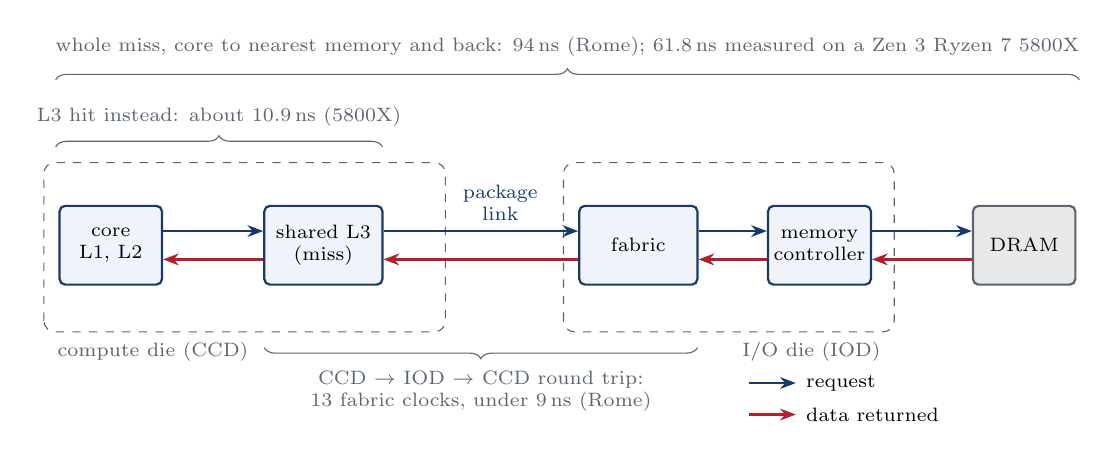
\begin{tikzpicture}[x=1cm,y=1cm,
  blk/.style={draw=draftblue,thick,fill=draftlight,rounded corners=2pt,font=\scriptsize,align=center,minimum height=1.0cm,inner sep=2pt},
  die/.style={draw=draftgray,dashed,rounded corners=4pt},
  req/.style={-{Stealth[length=2mm]},draftblue,thick},
  rsp/.style={-{Stealth[length=2mm]},todored,thick},
  note/.style={font=\scriptsize,align=center,text=draftgray}]
\draw[die] (-0.35,-0.9) rectangle (4.75,1.25);
\node[note,anchor=north west] at (-0.3,-0.9) {compute die (CCD)};
\draw[die] (6.25,-0.9) rectangle (10.45,1.25);
\node[note,anchor=north east] at (10.4,-0.9) {I/O die (IOD)};
\node[blk,minimum width=1.3cm] (core) at (0.5,0.2) {core\\L1, L2};
\node[blk,minimum width=1.5cm] (l3) at (3.2,0.2) {shared L3\\(miss)};
\node[blk,minimum width=1.5cm] (fab) at (7.2,0.2) {fabric};
\node[blk,minimum width=1.3cm] (umc) at (9.5,0.2) {memory\\controller};
\node[blk,minimum width=1.3cm,fill=draftgray!15,draw=draftgray] (dram) at (12.1,0.2) {DRAM};
\draw[req] ([yshift=0.18cm]core.east) -- ([yshift=0.18cm]l3.west);
\draw[req] ([yshift=0.18cm]l3.east) -- node[pos=0.6,above,align=center,font=\scriptsize,text=draftblue]{package\\link} ([yshift=0.18cm]fab.west);
\draw[req] ([yshift=0.18cm]fab.east) -- ([yshift=0.18cm]umc.west);
\draw[req] ([yshift=0.18cm]umc.east) -- ([yshift=0.18cm]dram.west);
\draw[rsp] ([yshift=-0.18cm]dram.west) -- ([yshift=-0.18cm]umc.east);
\draw[rsp] ([yshift=-0.18cm]umc.west) -- ([yshift=-0.18cm]fab.east);
\draw[rsp] ([yshift=-0.18cm]fab.west) -- ([yshift=-0.18cm]l3.east);
\draw[rsp] ([yshift=-0.18cm]l3.west) -- ([yshift=-0.18cm]core.east);
\draw[decorate,decoration={brace,amplitude=4pt,mirror},draftgray] (2.45,-1.1) -- (7.95,-1.1)
  node[midway,below=5pt,note]{CCD $\to$ IOD $\to$ CCD round trip:\\13 fabric clocks, under 9\,ns (Rome)};
\draw[decorate,decoration={brace,amplitude=4pt},draftgray] (-0.2,2.3) -- (12.8,2.3)
  node[midway,above=5pt,note]{whole miss, core to nearest memory and back: 94\,ns (Rome); 61.8\,ns measured on a Zen~3 Ryzen~7 5800X};
\draw[decorate,decoration={brace,amplitude=4pt},draftgray] (-0.2,1.45) -- (3.95,1.45)
  node[midway,above=4pt,note]{L3 hit instead: about 10.9\,ns (5800X)};
\draw[req] (8.6,-1.55) -- (9.2,-1.55) node[right,font=\scriptsize,text=black]{request};
\draw[rsp] (8.6,-1.95) -- (9.2,-1.95) node[right,font=\scriptsize,text=black]{data returned};
\end{tikzpicture}
\caption[The path of a load that misses in the L3 of a chiplet processor]{The path of a load that misses in the L3 of a chiplet processor. The request leaves the compute die, crosses the package link to the I/O die, where the memory controllers sit, and the data returns the same way. Times from AMD for Rome \cite{naffziger2020chiplet} and from AIDA64 measurements of the Ryzen~7 5800X \cite{justiceAMDRyzen72021}; the figures come from different processors and are shown for scale only.}
\label{fig:l3-miss-path}
\end{figure}


The central IOD also changed how uneven memory latency is across the socket. In the previous generation, Naples, each of four dies had its own memory controllers, so a core saw three different memory distances; Rome's single IOD reduced this to two (\cref{tab:numa-latency}).

\begin{table}[htbp]
  \centering
  \caption[Memory latency by NUMA distance, Naples and Rome, as reported by AMD]{Memory latency by NUMA distance, Naples (EPYC 7001) and Rome (EPYC 7002), as reported by AMD \cite[Fig.~2.2.6]{naffziger2020chiplet}.}
  \label{tab:numa-latency}
  \small
  \begin{tabular}{@{}lclc@{}}
    \toprule
    \multicolumn{2}{c}{\textbf{Naples: 8 NUMA domains, 3 distances}} & \multicolumn{2}{c}{\textbf{Rome: 2 NUMA domains, 2 distances}} \\
    \cmidrule(r){1-2}\cmidrule(l){3-4}
    Domain & Latency (ns) & Domain & Latency (ns) \\
    \midrule
    NUMA1 & 90 & Near 2 channels & 94 \\
    NUMA2 & 141 & NUMA1 & 104 \\
    NUMA3 & 234 & NUMA2 & 201 \\
    Average local & 128 & Local average vs Naples & 0.81$\times$ \\
    \bottomrule
  \end{tabular}
\end{table}
\Cref{fig:numa-latency} plots these numbers so that what the table lists can be seen at once: Rome's nearest access is slightly slower than Naples's, but its latencies span a much narrower range.

\begin{figure}[htbp]
\centering
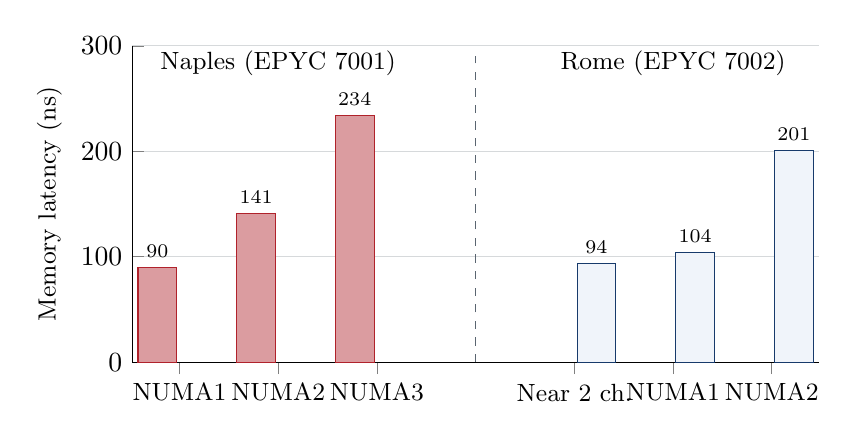
\begin{tikzpicture}
\begin{axis}[
  ybar, bar width=14pt, width=0.85\textwidth, height=5.6cm,
  ymin=0, ymax=300, ylabel={Memory latency (ns)},
  symbolic x coords={N1,N2,N3,gap,R1,R2,R3},
  xtick={N1,N2,N3,R1,R2,R3},
  xticklabels={NUMA1,NUMA2,NUMA3,{Near 2 ch.},NUMA1,NUMA2},
  x tick label style={font=\small},
  nodes near coords, nodes near coords style={font=\scriptsize},
  ymajorgrids, grid style={draftgray!25}, axis x line*=bottom, axis y line*=left,
  enlarge x limits=0.08, label style={font=\small}]
\addplot[fill=todored!45,draw=todored] coordinates {(N1,90) (N2,141) (N3,234)};
\addplot[fill=draftlight,draw=draftblue] coordinates {(R1,94) (R2,104) (R3,201)};
\node[font=\small,anchor=south] at (axis cs:N2,262) {Naples (EPYC 7001)};
\node[font=\small,anchor=south] at (axis cs:R2,262) {Rome (EPYC 7002)};
\draw[draftgray,dashed] (axis cs:gap,0) -- (axis cs:gap,290);
\end{axis}
\end{tikzpicture}
\caption[Memory latency at each NUMA distance in Naples and Rome, as reported by AMD]{Memory latency at each NUMA distance in Naples and Rome, as reported by AMD \cite[Fig.~2.2.6]{naffziger2020chiplet} (labels as in \cref{tab:numa-latency}). Rome's nearest access is slightly slower, probably because every memory access crosses the package link to the I/O die, but the spread of latencies within the socket is much narrower, and the average local latency fell to 0.81 of Naples's.}
\label{fig:numa-latency}
\end{figure}


The fastest access became slightly slower (94 against 90\,ns), probably because every memory access now crosses the IFOP link to the IOD. AMD nevertheless reports that the average fell by 19\%, which it attributes to the central I/O die together with decoupled clocks and the latency-optimised link; no access now has to cross to another compute die's memory controller inside the socket. This is the trade the chiplet organisation makes: a small penalty paid by every memory access in place of large, uneven ones.

\textbf{Bandwidth.} A single link limits how much memory bandwidth one CCD can draw. As an illustration, eight 64-bit DDR4-3200 channels, the configuration of both Rome and the most common EPYC~7003 systems \cite[slide~19]{suggs2019zen2}, \cite{amd2022epyc7003}, provide $8 \times 3200 \times 10^6 \times 8\,\mathrm{B} = 204.8$\,GB/s at peak, the figure AMD gives for Rome \cite[slide~19]{suggs2019zen2}. The desktop Matisse part has two such channels and 51.2\,GB/s \cite[slide~15]{suggs2019zen2}; with two CCDs and 16 cores that is $51.2/16 = 3.2$\,GB/s per core, exactly the share of a fully loaded 64-core Rome ($204.8/64$). The memory system was scaled with the number of compute dies, not the other way round. Naffziger \emph{et al.} give about 55\,GB/s of effective bandwidth per Rome CCD link \cite{naffziger2020chiplet}, roughly a quarter of that figure. Both numbers now describe Rome, but one is a peak rate and the other an effective rate, so the ratio is only indicative. It is, however, consistent with AMD's statement that at least four CCDs are populated in most Rome configurations to balance overall bandwidth \cite{naffziger2020chiplet}.

\textbf{Power.} Moving a bit across the package costs more energy than moving it across a die, because the link drives longer, more capacitive wires (\cref{eq:pdyn}) and needs serialisers and receivers at each end. AMD reports about 2\,pJ/bit for the predecessor link and states that the Rome link was designed to minimise power, avoiding active equalisation for that reason \cite{naffziger2020chiplet}. At 55\,GB/s, 2\,pJ/bit would correspond to roughly $55 \times 10^9 \times 8 \times 2 \times 10^{-12} \approx 0.9$\,W per fully loaded link; this is an order-of-magnitude illustration using the older generation's efficiency, not a measured Rome figure.

\subsection{Sharing data across dies}
\label{sec:cross-ccd}
The hop on an L3 miss is paid once per miss. Sharing between cores on different CCDs is costlier, because a block that two threads write in turn moves between their caches each time (\cref{tab:msi-example}), and in a chiplet processor every such move between CCDs passes through the I/O die. Part~\ref{part:foundations} showed that a directory protocol adds steps that go through a third party (\cref{tab:directory-example}); if the directory sat on another die, each of those steps would also cross the package, although the sources do not say where AMD keeps it (\cref{sec:multicore}).

Reguly measured what this costs on a Milan-X processor, an EPYC~7V73X with 3D V-Cache, running as an Azure virtual machine with SMT disabled \cite{regulyComparativeEvaluationBandwidthbound2023}. The test passes messages between two cores through shared cache lines, one core writing and the other reading, which is the access pattern of \cref{tab:msi-example}. \Cref{tab:core-to-core} gives the results, together with the same test on two Intel Xeon processors.

\begin{table}[htbp]
  \centering
  \caption[Core-to-core message-passing latency (Reguly)]{Message-passing latency between cores through shared cache lines (one writer, one reader), read from Reguly's Fig.~2 \cite{regulyComparativeEvaluationBandwidthbound2023}. The EPYC system ran as a cloud virtual machine with SMT disabled; the Intel columns' first row is between two hardware threads of one core.}
  \label{tab:core-to-core}
  \small
  \begin{tabularx}{\textwidth}{@{}>{\raggedright\arraybackslash}X ccc@{}}
    \toprule
    \textbf{Pair of cores} & \textbf{EPYC 7V73X} & \textbf{Xeon Platinum 8360Y} & \textbf{Xeon Max 9480} \\
    \midrule
    Two threads of one core & (SMT off) & 0.1\,ns & 0.7\,ns \\
    Adjacent cores (EPYC: same CCD) & 58.6\,ns & 106.1--109.5\,ns & 83.6--84.4\,ns \\
    EPYC: different CCD, same socket & 265.2--266.2\,ns & --- & --- \\
    Other socket & 396.9--415.3\,ns & 228.3--233.9\,ns & 241.6--246.6\,ns \\
    \bottomrule
  \end{tabularx}
\end{table}

Sharing \emph{within} a CCD is fast: at 58.6\,ns, two cores that share the CCD's L3 exchange data faster than adjacent cores on either Intel processor. Sharing \emph{across} CCDs takes about 4.5 times as long as within one, and on this system a core on another CCD in the same socket is farther away (265\,ns) than a core on the other socket of either Intel machine (228--247\,ns). Crossing to the other EPYC socket costs about 1.5 times the cross-CCD figure; Reguly reports the cross-socket figure as 1.6 times worse than on the Intel systems and warns that the virtual machine may have affected the results \cite{regulyComparativeEvaluationBandwidthbound2023}. The processors also differ in clock, core count and generation, so the comparison between vendors is indicative only. The comparison between rows of the EPYC column is cleaner, because all three were measured on the same system.

The group's own Ryzen~5 5600X gives a comparable same-CCD figure. Its six cores share one CCD, and in the group's ping-pong test (\cref{app:5600x}) a cache line passed from one core to another in about 49\,ns, half of a 98.5\,ns round trip, the same order as Reguly's 58.6\,ns. Like Reguly's, the measurement ran in a virtual machine, and the two tests time slightly different things, so the agreement is one of magnitude. The 5600X has a single CCD, so it cannot measure the cost of crossing between CCDs.

The extra cost of crossing CCDs, about $265 - 59 \approx 206$\,ns, is about eleven times the 18\,ns that the link itself accounts for. AMD gives under 9\,ns for one round trip between a CCD and the I/O die on Rome (\cref{sec:d2d}), and a request from one CCD to another and its reply cross that link four times, two such round trips. The link itself is therefore not most of the cost. A transfer between CCDs also has to pass through the fabric on the I/O die and through the steps of the coherence protocol at each end, and the sources used here do not break the total down. The figure is also not the same as the latency of a single miss: the test measures how long one message takes to travel from writer to reader, which includes the invalidation and the transfer.

For two threads that hand one shared block, such as a counter or a lock, back and forth two million times, the latencies of \cref{tab:core-to-core} give about 0.12\,s on one CCD, 0.53\,s across CCDs and 0.80\,s across sockets. The work is the same in all three cases; only the placement differs. A program that shares data heavily between threads can therefore run several times slower if the operating system spreads those threads across CCDs. This is the practical reason behind the NUMA options of \cref{sec:ccd-iod}: when EPYC~7003 exposes each CCD's L3 as a separate NUMA domain \cite{amd2022epyc7003}, the operating system and the programmer can see the boundary and keep threads that communicate on the same die. Programs that share little, such as many independent requests or processes, are hardly affected, which is the loosely coupled use that Amdahl's law favours (\cref{sec:multicore}).

A stacked cache does not change this cost. The V-Cache enlarges each CCD's L3 but leaves the path between CCDs as it was, and the EPYC~7V73X in \cref{tab:core-to-core} is itself a V-Cache part. What a larger L3 can change is how often a thread needs data held elsewhere: if more of its working set fits on its own CCD, fewer of its accesses leave the die at all.

\subsection{Scalability}
The chiplet organisation scales by adding compute dies, but the IOD is shared. Adding CCDs increases core count and total L3 capacity, while memory channels and I/O stay fixed by the IOD and the socket. As more cores share the same memory bandwidth, the bandwidth per core falls, which raises the value of a large L3 that keeps traffic off the memory channels. AMD's own Rome rule of thumb, at least four populated CCDs for bandwidth balance \cite{naffziger2020chiplet}, shows the opposite limit: with too few CCDs, the per-CCD links rather than the memory channels become the bottleneck. A star of point-to-point links to one IOD also has a fixed number of link ports, so the number of CCDs is bounded by the IOD design as well as by package area.

\subsubsection*{Balancing link and memory bandwidth}
\label{sec:bandwidth-example}
Naffziger \emph{et al.} give about 55\,GB/s of effective bandwidth per Rome IFOP link and state that at least four CCDs are populated in most configurations to balance overall bandwidth \cite{naffziger2020chiplet}. \Cref{tab:bandwidth-balance} shows why, comparing the total link bandwidth with the 205\,GB/s peak of eight DDR4-3200 channels computed above. As before, the link figure is effective and the memory figure is peak, so the comparison is indicative only.

\begin{table}[htbp]
  \centering
  \caption[Total CCD--IOD link bandwidth against peak memory bandwidth]{Total CCD--IOD link bandwidth against peak memory bandwidth (55\,GB/s per link \cite{naffziger2020chiplet}; 8 channels of DDR4-3200).}
  \label{tab:bandwidth-balance}
  \small
  \begin{tabular}{@{}ccccc@{}}
    \toprule
    \textbf{CCDs} & \textbf{Cores} & \textbf{Total link bandwidth} & \textbf{Limiting side} & \textbf{Memory bandwidth per core} \\
    \midrule
    2 & 16 & 110\,GB/s & links & $110/16 \approx 6.9$\,GB/s \\
    4 & 32 & 220\,GB/s & roughly balanced & $205/32 \approx 6.4$\,GB/s \\
    8 & 64 & 440\,GB/s & memory channels & $205/64 \approx 3.2$\,GB/s \\
    \bottomrule
  \end{tabular}
\end{table}
\Cref{fig:bandwidth-balance} extends the table to every CCD count from one to eight. It shows where the two limits cross, at about 3.7 CCDs, which the table's three rows only bracket.

\begin{figure}[htbp]
\centering
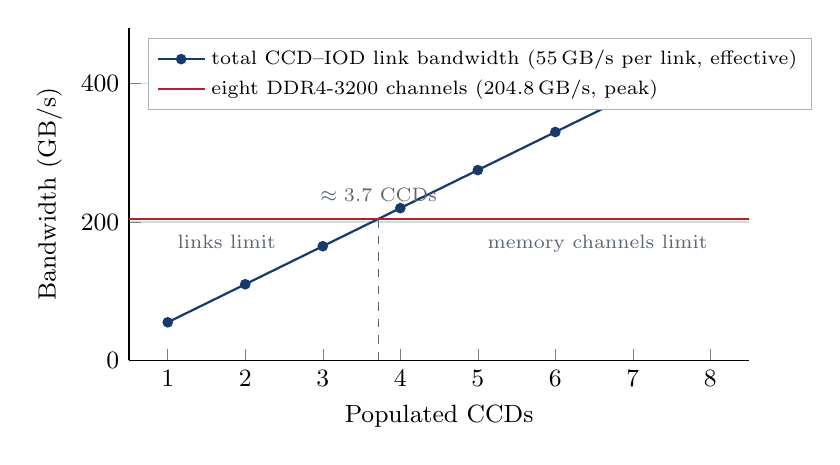
\begin{tikzpicture}
\begin{axis}[
  width=0.78\textwidth, height=5.8cm,
  xmin=0.5, xmax=8.5, ymin=0, ymax=480, xtick={1,...,8},
  xlabel={Populated CCDs}, ylabel={Bandwidth (GB/s)},
  ymajorgrids, grid style={draftgray!25}, axis x line*=bottom, axis y line*=left,
  legend pos=north west, legend cell align=left, legend style={font=\scriptsize,draw=draftgray!50},
  label style={font=\small}, tick label style={font=\small}]
\addplot[draftblue,thick,mark=*,mark size=1.5pt] coordinates {(1,55)(2,110)(3,165)(4,220)(5,275)(6,330)(7,385)(8,440)};
\addlegendentry{total CCD--IOD link bandwidth ($55$\,GB/s per link, effective)}
\addplot[todored,thick,domain=0.5:8.5] {204.8};
\addlegendentry{eight DDR4-3200 channels ($204.8$\,GB/s, peak)}
\addplot[draftgray,dashed] coordinates {(3.72,0)(3.72,204.8)};
\node[font=\scriptsize,anchor=north west,text=draftgray,align=left] at (axis cs:1.0,195) {links limit};
\node[font=\scriptsize,anchor=north west,text=draftgray,align=left] at (axis cs:5.0,195) {memory channels limit};
\node[font=\scriptsize,anchor=south,text=draftgray] at (axis cs:3.72,215) {$\approx 3.7$ CCDs};
\end{axis}
\end{tikzpicture}
\caption[Which side limits a Rome socket's memory bandwidth as compute dies are added]{Which side limits a Rome socket's memory bandwidth as compute dies are added: below about four CCDs the die-to-die links are the bottleneck, above it the memory channels. This is consistent with AMD's statement that at least four CCDs are populated in most configurations \cite{naffziger2020chiplet}. The link figure is effective and the memory figure peak, so the crossing point is indicative (\cref{tab:bandwidth-balance}).}
\label{fig:bandwidth-balance}
\end{figure}


With two CCDs the links, not the memory, are the bottleneck; at four the two sides are roughly matched, which is AMD's rule of thumb; at eight, the memory channels limit, and each core's share of memory bandwidth halves. The last column is the point that connects Part~\ref{part:chiplets} to Part~\ref{part:stacked-cache}: the more cores share a socket's memory channels, the more valuable it is to satisfy requests from a large on-package cache instead.

\subsubsection*{Scaling beyond one socket}
The same links extend to two sockets. Two identical EPYC~7003 processors connect through their external Global Memory Interconnect (xGMI) Infinity Fabric links, which use the same physical connections as the PCIe lanes \cite{amd2022epyc7003}. Each link uses 16 lanes, so a socket that devotes four links to the other socket gives up 64 of its 128 lanes, leaving $2 \times 64 = 128$ lanes for the whole system. A designer who uses three links instead frees $128 - 48 = 80$ lanes per socket, 160 in total, at the cost of inter-socket bandwidth \cite{amd2022epyc7003}. A dual-socket system has sixteen memory channels and can be configured with between 1 and 16 NUMA domains. The trade between I/O lanes and inter-processor bandwidth is the package-level version of the trade between link width and die area seen within the package (\cref{sec:packaging-options}). \Cref{fig:two-socket} shows the two configurations.

\begin{figure}[htbp]
\centering
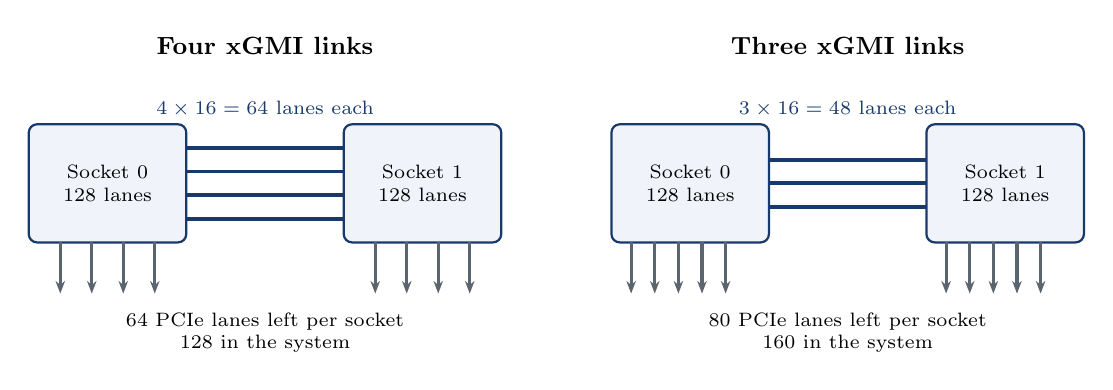
\begin{tikzpicture}[x=1cm,y=1cm,
  pkg/.style={draw=draftblue,thick,fill=draftlight,rounded corners=3pt,minimum width=2.0cm,minimum height=1.5cm,font=\scriptsize,align=center},
  lnk/.style={draftblue,line width=1.4pt},
  io/.style={draftgray,line width=1.1pt,-{Stealth[length=1.6mm]}},
  note/.style={font=\scriptsize,align=center}]
\begin{scope}
  \node[font=\small\bfseries] at (2.0,1.75) {Four xGMI links};
  \node[pkg] (A) at (0,0) {Socket 0\\128 lanes};
  \node[pkg] (B) at (4,0) {Socket 1\\128 lanes};
  \foreach \y in {-0.45,-0.15,0.15,0.45} \draw[lnk] (1.0,\y) -- (3.0,\y);
  \node[note,text=draftblue] at (2,0.95) {$4 \times 16 = 64$ lanes each};
  \foreach \x in {-0.6,-0.2,0.2,0.6} {\draw[io] (\x,-0.75) -- (\x,-1.4); \draw[io] (4+\x,-0.75) -- (4+\x,-1.4);}
  \node[note] at (2,-1.9) {64 PCIe lanes left per socket\\128 in the system};
\end{scope}
\begin{scope}[xshift=7.4cm]
  \node[font=\small\bfseries] at (2.0,1.75) {Three xGMI links};
  \node[pkg] (C) at (0,0) {Socket 0\\128 lanes};
  \node[pkg] (D) at (4,0) {Socket 1\\128 lanes};
  \foreach \y in {-0.3,0,0.3} \draw[lnk] (1.0,\y) -- (3.0,\y);
  \node[note,text=draftblue] at (2,0.95) {$3 \times 16 = 48$ lanes each};
  \foreach \x in {-0.75,-0.45,-0.15,0.15,0.45} {\draw[io] (\x,-0.75) -- (\x,-1.4); \draw[io] (4+\x,-0.75) -- (4+\x,-1.4);}
  \node[note] at (2,-1.9) {80 PCIe lanes left per socket\\160 in the system};
\end{scope}
\end{tikzpicture}
\caption[The lane trade in a dual-socket EPYC~7003 system]{The lane trade in a dual-socket EPYC~7003 system: the links between sockets (xGMI, blue) use the same 16-lane connections as PCIe, so each link given to the other socket removes 16 lanes of I/O (grey arrows, schematic) \cite{amd2022epyc7003}. Fewer links mean more I/O but less bandwidth between the sockets.}
\label{fig:two-socket}
\end{figure}


\subsection{How the dies are connected: organic substrate, 2.5D and 3D}
\label{sec:packaging-options}
Chiplets can be joined in three broad ways, which differ mainly in how finely their connections can be spaced (\cref{tab:packaging-levels}).\index{2.5D integration}
\begin{itemize}
  \item \textbf{On the organic package substrate} (a multi-chip module, sometimes called 2D packaging). Each die is mounted on the substrate with C4 solder bumps, and the substrate's copper traces connect the dies. This is the cheapest option and allows long links, but the connections are coarse.
  \item \textbf{2.5D integration.} The dies still sit side by side, but they are joined through a finer layer of wiring placed under or between them: a silicon interposer, a small embedded silicon bridge, or a fan-out redistribution layer. Connections are much denser, so a link of the same width carries more bandwidth with less energy per bit, but the extra silicon adds cost and limits how far apart the dies can be.
  \item \textbf{3D integration.} One die is stacked directly on another and connected through through-silicon vias (TSVs) and micro-bumps or hybrid bonds (Part~\ref{part:stacked-cache}). This gives the densest and shortest connections.
\end{itemize}

\begin{table}[htbp]
  \centering
  \caption[Die-to-die connection methods]{Die-to-die connection methods, with AMD's interconnect pitch targets \cite[slide~13]{lambertHeterogenousIntegrationHigh2025} and AMD examples.}
  \label{tab:packaging-levels}
  \small
  \begin{tabularx}{\textwidth}{@{}>{\raggedright\arraybackslash}p{2.6cm}>{\raggedright\arraybackslash}p{1.8cm}>{\raggedright\arraybackslash}X>{\raggedright\arraybackslash}X@{}}
    \toprule
    \textbf{Method} & \textbf{Pitch} & \textbf{AMD examples} & \textbf{Main trade-off} \\
    \midrule
    Organic substrate (C4 bumps) & $<150$\,\textmu m & EPYC~7002 and Ryzen~3000 CCD--IOD links \cite{naffziger2020chiplet} & long reach and low cost; coarse links \\
    2.5D (interposer, bridge or fan-out) & $<40$\,\textmu m & Fiji GPU with high-bandwidth memory (HBM) on a silicon interposer (2015) \cite[slide~9]{swaminathanAdvancedPackagingEnabling2021}; Ryzen~AI~Max~PRO~300 \cite[slide~8]{lambertHeterogenousIntegrationHigh2025} & denser, lower-energy links; added silicon and shorter reach \\
    3D (hybrid bonding) & $<9$\,\textmu m & 3D V-Cache \cite{wuu2022vcache} & densest, shortest links; heat and test complexity \\
    \bottomrule
  \end{tabularx}
\end{table}

AMD's choice for its chiplet CPUs was deliberate. Naffziger \emph{et al.} contrast the organic-package SerDes link with a 2.5D interposer and with Intel's embedded bridge (EMIB), and state that its key benefit is longer reach, which allowed chiplets to be arranged in columns two deep; without that, eight CCDs would not have fitted around one IOD \cite{naffziger2020chiplet}. Rome and Matisse therefore connect their CCDs to the IOD through the organic substrate, and the later Zen CPUs studied in this paper use 3D stacking for the extra cache; the sources used here do not describe a change to the CCD--IOD connection in those later generations (\cref{sec:d2d}, Part~\ref{part:stacked-cache}).

\begin{figure}[htbp]
\centering
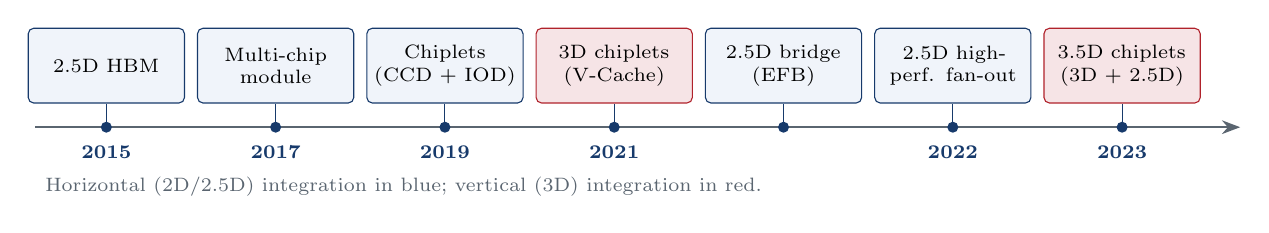
\begin{tikzpicture}[x=1cm,y=1cm,
  ev/.style={draw=draftblue,fill=draftlight,rounded corners=2pt,font=\scriptsize,align=center,text width=1.75cm,minimum height=0.95cm},
  ev3/.style={ev,fill=todored!12,draw=todored},
  yr/.style={font=\scriptsize\bfseries,text=draftblue}]
\draw[-{Stealth},thick,draftgray] (-0.3,0) -- (15.0,0);
\foreach \x/\y/\t/\s in {0.6/2015/2.5D HBM/ev, 2.75/2017/Multi-chip module/ev, 4.9/2019/Chiplets (CCD + IOD)/ev, 7.05/2021/3D chiplets (V-Cache)/ev3, 9.2//2.5D bridge (EFB)/ev, 11.35/2022/2.5D high-perf. fan-out/ev, 13.5/2023/3.5D chiplets (3D + 2.5D)/ev3}{
  \fill[draftblue] (\x,0) circle (0.07);
  \node[yr,below] at (\x,-0.12) {\y};
  \node[\s,above] at (\x,0.3) {\t};
  \draw[draftblue] (\x,0.07) -- (\x,0.3);}
\node[font=\scriptsize,text=draftgray,anchor=west] at (-0.3,-0.75) {Horizontal (2D/2.5D) integration in blue; vertical (3D) integration in red.};
\end{tikzpicture}
\caption[AMD's packaging steps as presented by AMD]{AMD's packaging steps as presented by AMD \cite[slide~5]{lambertHeterogenousIntegrationHigh2025}. The slide gives no separate year for the 2.5D bridge (EFB). The CPUs studied in this paper use the 2019 chiplet organisation and, from 2021, 3D-stacked cache.}
\label{fig:packaging-timeline}
\end{figure}

2.5D integration is nevertheless part of AMD's wider packaging history (\cref{fig:packaging-timeline}). Its own timeline runs from 2.5D HBM (2015) through the multi-chip module (2017), chiplets (2019) and 3D chiplets (2021) to a 2.5D bridge (labelled EFB on AMD's slide), 2.5D high-performance fan-out (2022) and ``3.5D'' chiplets (2023) \cite[slide~5]{lambertHeterogenousIntegrationHigh2025}. The Instinct MI300 accelerator combines both: dies hybrid-bonded on top of I/O dies, which sit side by side on a 2.5D silicon interposer \cite[slide~10]{lambertHeterogenousIntegrationHigh2025}. Among Zen-based processors, the Ryzen~AI~Max~PRO~300 series uses 2.5D fan-out packaging, which AMD describes as a ``continued strategic use of 2.5D advanced packaging to reduce die-to-die power and latency'' \cite[slide~8]{lambertHeterogenousIntegrationHigh2025}. Swaminathan names the parameters that decide between these options: cost and volume, \emph{bandwidth density} (the area spent on die-to-die communication) and \emph{energy per bit} \cite[slide~7]{swaminathanAdvancedPackagingEnabling2021}. The organic substrate wins on cost and reach, 2.5D on bandwidth density and energy, and 3D on both of the latter at the price of the thermal and manufacturing issues of \cref{sec:thermal}.

\section{Yield, Process-Node Specialisation and Cost}
\label{sec:process-specialisation}

Chiplets combine two cost advantages. First, small dies yield better (\cref{sec:yield-cost}). Second, each die can use the process that suits it: AMD keeps memory interfaces and SerDes on 12\,nm because they would see little benefit at 7\,nm \cite{naffziger2020chiplet}. AMD also tests every CCD before assembly (\cref{sec:chiplet-power}), which limits the cost of combining several dies in one package.

These benefits are not free. AMD describes the design as requiring package--silicon co-design, new interconnect circuits, a mixed-process package (with copper pillars on the 12\,nm IOD to match die heights), and new test and power-management infrastructure \cite{naffziger2020chiplet}.

The model of \cref{app:yield-cost} gives a rough sense of the silicon saving. Consider eight Rome-sized CCDs of 74\,mm$^2$ each, 592\,mm$^2$ in total, against a hypothetical monolithic die with the same compute area (ignoring the I/O, which in the chiplet design moves to a cheaper node). With $D_0 = 0.2$\,cm$^{-2}$ and the yield model of \cref{eq:yield}, a 74\,mm$^2$ CCD yields about 87\% and the 592\,mm$^2$ die about 38\%, so eight tested CCDs cost about 44\% of the silicon of one good monolithic die; with $D_0 = 0.1$\,cm$^{-2}$ the figure is about 63\%. These numbers are illustrative only: they ignore interface area, packaging, assembly yield and test cost, and Dong and Xie find an analogous effect for 3D stacking, where the extra bonding and test costs outweigh the yield gain for small designs, so that stacking pays only above a size threshold \cite{dongSystemlevelCostAnalysis2009}. They also ignore the separate saving from building the I/O on a mature node \cite{naffziger2020chiplet}. The qualitative conclusion is robust, however: for a design of server size, the yield advantage of small dies is large.

Yield is only half of the cost story; the other half is how many dies fit on a wafer, which falls faster than area because partial dies are lost around the circular edge. Counting both (\cref{app:dies-per-wafer}), a 300\,mm wafer of 74\,mm$^2$ CCDs supplies the compute silicon for about 95 64-core processors, against 35 for a 592\,mm$^2$ monolithic die, a factor of 2.7 (1.9 with $D_0 = 0.1$, 3.5 with $D_0 = 0.3$). The calculation ignores the I/O die, packaging and test, and assumes that such a large die could be made at all.

AMD's own estimate points the same way (\cref{fig:chiplet-cost-chart}). Naffziger \emph{et al.} compare the cost of Rome chiplet products with hypothetical monolithic 7\,nm designs of the same core count \cite[Fig.~2.2.2]{naffziger2020chiplet}. Read from the chart, the monolithic designs cost roughly twice as much at 48 and 32 cores and about 1.8$\times$ at 16 cores, and the chiplet design scales its cost down with core count by leaving CCD positions empty (``depopulation'') and using partly defective dies (``harvesting''). Two details of the chart should be noted: its legend describes the chiplet design as ``7\,nm + 14\,nm'', whereas the paper's text gives 12\,nm for the I/O die, and the chart's axis is a normalised cost without units. The chart is AMD's model, not a disclosed cost, but its factor of about two agrees with the order of magnitude of \cref{tab:dies-per-wafer}.

\begin{figure}[htbp]
\centering
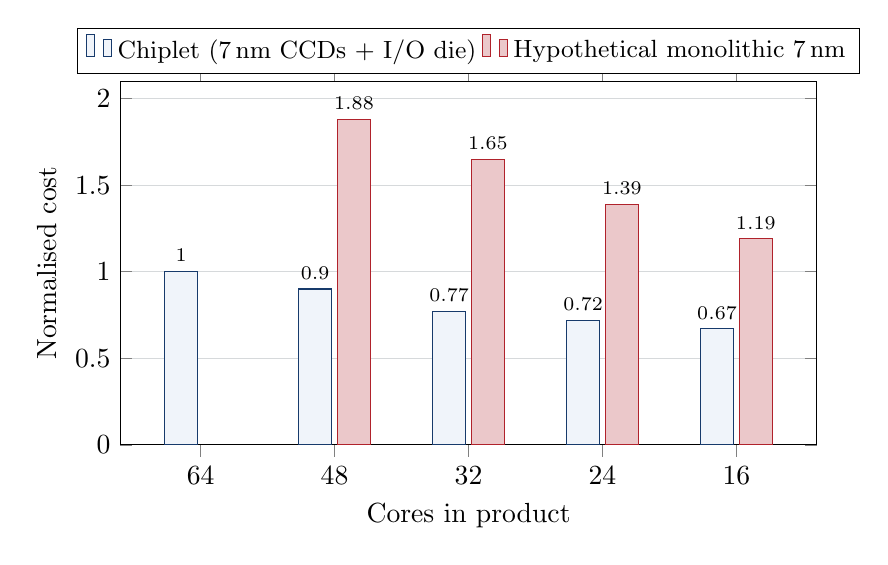
\begin{tikzpicture}
\begin{axis}[
  ybar, bar width=12pt, width=0.86\textwidth, height=6.2cm,
  ymin=0, ymax=2.1, ylabel={Normalised cost},
  symbolic x coords={64,48,32,24,16}, xtick=data, xlabel={Cores in product},
  legend style={font=\small,at={(0.5,1.02)},anchor=south,legend columns=2},
  ymajorgrids, grid style={draftgray!25}, enlarge x limits=0.15,
  nodes near coords, nodes near coords style={font=\scriptsize}, every node near coord/.append style={/pgf/number format/fixed,/pgf/number format/precision=2}]
\addplot[fill=draftlight,draw=draftblue] coordinates {(64,1.00) (48,0.90) (32,0.77) (24,0.72) (16,0.67)};
\addplot[fill=todored!25,draw=todored] coordinates {(48,1.88) (32,1.65) (24,1.39) (16,1.19)};
\legend{Chiplet (7\,nm CCDs + I/O die), Hypothetical monolithic 7\,nm}
\end{axis}
\end{tikzpicture}
\caption[Cost of chiplet and hypothetical monolithic Rome-generation products (AMD)]{Cost against core count for Rome-generation chiplet products and hypothetical monolithic 7\,nm equivalents, normalised to the 64-core chiplet part. Values were read by eye from AMD's chart \cite[Fig.~2.2.2]{naffziger2020chiplet} and are accurate only to about $\pm 0.05$. AMD shows no monolithic 64-core bar; the text states that such a die would exceed the maximum reticle size.}
\label{fig:chiplet-cost-chart}
\end{figure}

\section{Power, Clocking and Product Flexibility}
\label{sec:power-flexibility}
Research question RQ2 asks what the split into compute and I/O dies changes for power and for product flexibility as well as for latency and bandwidth. The evidence on the two is very different. On flexibility the AMD sources are detailed and the product lists can be checked; on power they describe design choices but give no measurement of the I/O die or of the package at idle.

\subsection{Power and clocking}
\label{sec:chiplet-power}
Two kinds of power cost come with the split. The first is the energy of the links, discussed in \cref{sec:d2d}: about 2\,pJ/bit for the predecessor link, with the Rome link designed to reduce it further by using single-ended signalling, a termination scheme that needs little power to maintain, no active equalisation and a bandwidth-limited clock distribution \cite{naffziger2020chiplet}. The second is that the I/O die is a separate chip with its own clocks and voltage. Here the chiplet design turned a cost into a control. In Naples, the clocks of the fabric, the memory and the inter-socket links were tied together; in Rome they can be set independently. AMD states that this clocking flexibility, together with dynamic voltage and frequency scaling (DVFS) of the uncore and a variable memory clock, enables power management that shifts power between the CPU cores and the uncore within a fixed thermal design power (TDP) \cite{naffziger2020chiplet}. The same source adds a qualification: Rome and Matisse have clocking modes that improve latency when the fabric clock equals the memory clock \cite{naffziger2020chiplet}, so decoupling the clocks saves power at some cost in latency. The Cezanne comparison of \cref{sec:cezanne}, where the 5700G ran a 1600\,MHz fabric clock against the 5800X's 1800\,MHz, shows how strongly such settings enter measured latencies.

Two further mechanisms let a chiplet product match its power to its configuration. AMD tests every CCD before assembly, and if a CCD is damaged during assembly, firmware ``down-bins'' it, putting the CCD and its interconnect logic into a known low-power state \cite{naffziger2020chiplet}. And in the fourth-generation EPYC processors, a CCD can connect to the I/O die through one link or two. Models with four or fewer CCDs use two links per CCD to double the bandwidth, while models with more CCDs use one. The I/O die's twelve links allow 4, 8 or 12 CCDs ``depending on the performance and power requirements'' of the product \cite{advancedmicrodevicesinc.4thGenAMD2023}.

\subsubsection*{How much power the links could take}
No source used here gives the power of the Rome or Genoa links, so this example estimates it with the one figure available, 2\,pJ/bit for the predecessor link \cite{naffziger2020chiplet}. Two observations make the estimate simple. A 64-byte line is 512 bits, so moving one line across a link costs about $512 \times 2\,\text{pJ} \approx 1$\,nJ. And memory traffic can cross the links no faster than the memory channels supply it.
\begin{itemize}
  \item \textbf{Rome}, eight channels of DDR4-3200 at 204.8\,GB/s (\cref{sec:d2d}): $204.8 \times 10^{9} \times 8 \times 2 \times 10^{-12} \approx 3.3$\,W with the memory fully loaded.
  \item \textbf{Genoa}, twelve channels of DDR5-4800 at 460.8\,GB/s \cite{advancedmicrodevicesinc.AMDEPYC90042023}: about 7.4\,W on the same assumption, against a default TDP of 360\,W for the 96-core EPYC~9654 \cite{advancedmicrodevicesinc.AMDEPYC90042023}, or about 2\%.
\end{itemize}
Traffic between CCDs, I/O and the link controllers' own idle power come on top, and newer links are probably more efficient per bit than the predecessor's, so these numbers are an order of magnitude, not a measurement. They suggest that the energy of moving memory data across the package is a small share of the processor's power budget. They do not show that the I/O die as a whole is cheap in power, because its memory controllers, fabric and I/O are not counted. The power side of RQ2 can therefore be answered only for link energy, and otherwise qualitatively, from the sources used in this paper.

\subsection{One compute die, many products}
\label{sec:product-flexibility}
The flexibility gain is easier to document. AMD describes three chiplets ``leveraged to many products and markets'' and states that the chiplet architecture brings leading-edge CPUs to several markets with high reuse for faster time-to-market \cite[Fig.~2.2.1]{naffziger2020chiplet}. The same CCD serves Rome and Matisse; different Rome models leave some CCD positions empty ``to optimize cost and performance''; and the client I/O die, packaged on its own, doubles as the X570 chipset \cite{naffziger2020chiplet}. The fourth-generation white paper calls the CPU die ``a unit of innovation'' that AMD can ``swap in and out'' to match products to workloads \cite{advancedmicrodevicesinc.4thGenAMD2023}.

\Cref{tab:product-matrix} tests the claim against AMD's own product lists. Each row is a product built from its generation's compute die. The number of CCDs and of active cores per CCD is not stated in the datasheets; the table infers it from the L3 size and the 32\,MB of L3 that each CCD carries in all three generations, two 16\,MB halves on Zen~2 and one 32\,MB L3 on Zen~3 and Zen~4, or 96\,MB with V-Cache \cite{suggs2019zen2,wuu2022vcache,advancedmicrodevicesinc.4thGenAMD2023}. The inference is unreliable when part of a CCD's L3 is disabled: the same datasheet lists an EPYC~9224 with 24 cores and 64\,MB, which by this rule would be two CCDs holding at most 16 cores \cite{advancedmicrodevicesinc.AMDEPYC90042023}. The configurations in the table are therefore plausible readings, not facts; only the EPYC~9174F's is stated by AMD.

\begin{table}[htbp]
  \centering
  \caption[One compute die, many products]{One compute die, many products: Zen~2 and Zen~3 desktop processors \cite{advancedmicrodevicesinc.AMDRyzen30002022} and Zen~4 server processors \cite{advancedmicrodevicesinc.AMDEPYC90042023}. CCDs $\times$ active cores inferred from the L3 size (32\,MB per CCD, 96\,MB with V-Cache), except where stated; the rule fails when L3 is partly disabled, as on the EPYC~9224 (24 cores, 64\,MB).}
  \label{tab:product-matrix}
  \small
  \begin{tabular}{@{}lccccc@{}}
    \toprule
    \textbf{Product} & \textbf{Cores} & \textbf{L3 (MB)} & \textbf{CCDs $\times$ cores} & \textbf{L3 per core} & \textbf{Default TDP} \\
    \midrule
    Ryzen~9 3950X / 5950X & 16 & 64 & $2 \times 8$ & 4\,MB & 105\,W \\
    Ryzen~9 3900X / 5900X & 12 & 64 & $2 \times 6$ & 5.3\,MB & 105\,W \\
    Ryzen~7 3800X / 5800X & 8 & 32 & $1 \times 8$ & 4\,MB & 105\,W \\
    Ryzen~5 3600 / 5600X & 6 & 32 & $1 \times 6$ & 5.3\,MB & 65\,W \\
    \midrule
    EPYC~9654 & 96 & 384 & $12 \times 8$ & 4\,MB & 360\,W \\
    EPYC~9554 & 64 & 256 & $8 \times 8$ & 4\,MB & 360\,W \\
    EPYC~9354 & 32 & 256 & $8 \times 4$ & 8\,MB & 280\,W \\
    EPYC~9334 & 32 & 128 & $4 \times 8$ & 4\,MB & 210\,W \\
    EPYC~9124 & 16 & 64 & $2 \times 8$ & 4\,MB & 200\,W \\
    EPYC~9174F & 16 & 256 & $8 \times 2$ (stated) & 16\,MB & 320\,W \\
    EPYC~9684X (V-Cache) & 96 & 1152 & $12 \times 8$ & 12\,MB & 400\,W \\
    EPYC~9184X (V-Cache) & 16 & 768 & $8 \times 2$ & 48\,MB & 320\,W \\
    \bottomrule
  \end{tabular}
\end{table}

The table shows how wide a range one die design covers. The Zen~4 server products in the table alone span 16 to 96 cores, 64\,MB to 1152\,MB of L3 and 4 to 48\,MB of L3 per core, with only two variants of the compute die (with and without the stacked cache) and one server I/O die. The datasheet's EPYC~9224 is lower, at 2.7\,MB per core \cite{advancedmicrodevicesinc.AMDEPYC90042023}, and the 112- and 128-core parts use a different, Zen~4c, compute die \cite{advancedmicrodevicesinc.4thGenAMD2023}. A monolithic product line would need a separate die for each core count or would have to disable cores on one large die, paying for silicon it does not sell. Products with fewer active cores per CCD also give a use for dies on which not every core is needed, and possibly for dies on which not every core works, although the sources used here do not say how AMD sorts its dies.

Two rows make a point that only chiplets can. The EPYC~9124 and 9174F both have 16 cores. AMD states that the 9174F spreads them over eight CCDs with two active cores each, and that this ``spreads the thermal load across the processor package and enables us to increase the clock frequency'', to a base of 4.10\,GHz against 3.00\,GHz \cite{advancedmicrodevicesinc.4thGenAMD2023}. The datasheet shows the cost: a default TDP of 320 against 200\,W \cite{advancedmicrodevicesinc.AMDEPYC90042023}. The spread also brings eight CCDs' worth of L3, 256\,MB against the 9124's 64\,MB \cite{advancedmicrodevicesinc.AMDEPYC90042023}, and eight links to the I/O die. On a single die, sixteen cores cannot be spread over eight dies' worth of area and cache; in a chiplet package, the number of dies becomes a design variable that trades power and price for clock, cache per core and bandwidth.

The same logic explains how 3D V-Cache entered the product lines. In EPYC~7003, the X-series models triple the L3 of the standard models using the same Zen~3 core \cite[sec.~1.1]{amd2022epyc7003}, and in EPYC~9004 three V-Cache models sit beside the standard ones \cite{advancedmicrodevicesinc.AMDEPYC90042023}. Because the stacked cache is a property of the CCD, AMD can offer it on a few products without designing a new processor, which is part of the answer to RQ3 as well as to RQ2 (Part~\ref{part:stacked-cache}).

\section{The Same Core With and Without Chiplets}
\label{sec:cezanne}
Zen~3 offers something close to a natural experiment. The same core appears in two desktop designs. Vermeer, the Ryzen~5000 series used throughout this paper, follows the chiplet organisation of this part: an eight-core CCD with 32\,MB of L3, joined through the package to a separate I/O die. Cezanne, the Ryzen~5000G series, places eight Zen~3 cores, a 16\,MB L3, the memory controllers and integrated graphics on one monolithic die, the same die AMD uses in its mobile processors \cite{waltonAMDRyzen72021}. If the die-to-die hop of \cref{sec:d2d} were a large cost, Cezanne should show it by its absence. \Cref{tab:cezanne-vermeer} collects what the sources measured.

\begin{table}[htbp]
  \centering
  \caption[Zen~3 with and without the chiplet split: Cezanne against Vermeer and Milan]{Zen~3 with and without the chiplet split: Cezanne (monolithic) against Vermeer and Milan (chiplet). Values come from different tools, memory settings and processors, as stated in each cell; they are not a controlled comparison.}
  \label{tab:cezanne-vermeer}
  \small
  \begin{tabularx}{\textwidth}{@{}>{\raggedright\arraybackslash}p{2.7cm}>{\raggedright\arraybackslash}X>{\raggedright\arraybackslash}X@{}}
    \toprule
    & \textbf{Cezanne (one die)} & \textbf{Vermeer / Milan (CCD + I/O die)} \\
    \midrule
    L3 per eight cores & 16\,MB & 32\,MB \\
    Boost clock; TDP & 4.6\,GHz; 65\,W (5700G) \cite{waltonAMDRyzen72021} & 4.7\,GHz; 105\,W (5800X) \cite{waltonAMDRyzen72021} \\
    PCIe & 3.0 \cite{waltonAMDRyzen72021} & 4.0 \cite{waltonAMDRyzen72021} \\
    L3 hit latency & 47 cycles (5600G, pointer chase) \cite{7-cpu.comAMDZen3}; 12.6\,ns, about 50 cycles (5700G at 4\,GHz, AIDA64) \cite{devtechprofileWhomCezanneCould2021} & 47.49 cycles (Milan, same CCD design) \cite{cozmaAMDsVCacheTested2022}; about 53 cycles from 10.9\,ns (5800X, AIDA64) \cite{justiceAMDRyzen72021} \\
    Memory latency & 76.1\,ns (5700G at 4\,GHz, AIDA64, DDR4-3200 CL16, 1600\,MHz fabric clock) \cite{devtechprofileWhomCezanneCould2021}; 47 cycles + 74\,ns, about 85\,ns (5600G, pointer chase, DDR4-3000 CL15, 2\,MB pages) \cite{7-cpu.comAMDZen3} & 61.8\,ns (5800X, AIDA64, DDR4-3600 CL16, 1800\,MHz fabric clock) \cite{justiceAMDRyzen72021} \\
    Memory latency, same memory and clock & \multicolumn{2}{>{\raggedright\arraybackslash}p{9.6cm}}{5700G against a 3950X with one CCD active, both at 4\,GHz with the same DDR4-3200 CL16 kit: ``very similar'' (only the 5700G's value, 76.1\,ns, is shown) \cite{devtechprofileWhomCezanneCould2021}} \\
    Performance, 5700G against 5800X & \multicolumn{2}{>{\raggedright\arraybackslash}p{9.6cm}}{Cinebench R20 multi-core about 10\% lower; 7-Zip compression 9\% lower; games at 1080p with an RTX~3090 11\% lower on average (4--20\% by title); total system power about 15\% lower \cite{waltonAMDRyzen72021}} \\
    \bottomrule
  \end{tabularx}
\end{table}

\textbf{L3 latency does not depend on the split.} The monolithic Cezanne and the chiplet-based Milan reach their L3 in about the same number of cycles, 47 against 47.5 by pointer chasing, although Cezanne's L3 is half the size \cite{7-cpu.comAMDZen3,cozmaAMDsVCacheTested2022}. AIDA64 gives a similar match, about 50 cycles on the 5700G at 4\,GHz against about 53 on the 5800X \cite{devtechprofileWhomCezanneCould2021,justiceAMDRyzen72021}. This is what the organisation predicts: in both designs the L3 sits beside the cores on the same die, so the chiplet boundary lies beyond it. The 7-cpu measurements also show where the cycles go on Cezanne: about 40 cycles to the nearest of the eight L3 slices, plus up to 20 more for the farthest \cite{7-cpu.comAMDZen3}, the slice-and-ring structure of \cref{fig:l3-slices}. Halving the capacity of each slice did not shorten the trip around the ring.

\textbf{Memory latency: no advantage for the single die.} Measured with the same tool, AIDA64, the monolithic 5700G took 76.1\,ns to reach memory and the chiplet-based 5800X 61.8\,ns \cite{devtechprofileWhomCezanneCould2021,justiceAMDRyzen72021}. That is the opposite of what removing the die-to-die hop would suggest, but the 5700G ran with slower memory (DDR4-3200 against DDR4-3600), a slower fabric clock (1600 against 1800\,MHz) and a lower core clock (4.0 against about 4.85\,GHz). CapFrameX notes that the core clock affects AIDA64's latency result and that AIDA64's absolute values have been criticised as too low \cite{devtechprofileWhomCezanneCould2021}. The difference therefore cannot be credited to the organisation. The one comparison with matched memory and clocks, by CapFrameX, found the 5700G's memory latency ``very similar'' to that of a chiplet-based Zen~2 part with one CCD active \cite{devtechprofileWhomCezanneCould2021}. CapFrameX offers an explanation from an annotated die photograph: even on Cezanne's single die, the memory controller is reached from the L3's ring of slices through the Infinity Fabric, and the transition from ring to fabric costs extra cycles \cite{devtechprofileWhomCezanneCould2021}. If that is right, putting everything on one die removes the package link but not the fabric, and the package link is the smaller part: AMD gives a round trip of 13 fabric clocks, under 9\,ns (\cref{fig:l3-miss-path}), roughly a tenth of a memory access of 60 to 90\,ns. The sources thus show no memory-latency advantage for the monolithic die, though none measures the two designs under identical conditions.

\textbf{Performance favours the chiplet part.} In TechSpot's tests the 5700G trailed the 5800X by about 10\% in multi-threaded applications and by 11\% on average in games, with the gap reaching 20\% in one title \cite{waltonAMDRyzen72021}. TechSpot does not report the clocks reached during its runs. The rated boost clocks differ by only about 2\% (4.6 against 4.7\,GHz), but measured clocks may differ more: CapFrameX saw the 5700G at 4.5--4.55\,GHz in games, and the 5800X ran at about 4.85\,GHz in The FPS Review's AIDA64 run, a gap of up to about 8\% \cite{devtechprofileWhomCezanneCould2021,justiceAMDRyzen72021}. Clock speed is nevertheless unlikely to explain most of the gaming gap: CapFrameX found that raising the 5700G's clock by more than 10\%, from a fixed 4\,GHz to its stock boost, gained only 3.22\% in games on average \cite{devtechprofileWhomCezanneCould2021}. Other differences remain: the 5700G has half the L3, a 65\,W rather than 105\,W TDP, and PCIe~3.0 rather than 4.0, and TechSpot measured about 15\% less power at the wall for the whole system \cite{waltonAMDRyzen72021}. The power limit can explain much of the multi-threaded gap, but games load fewer cores and are less limited by power. The reviewer's tentative reading is that, in CPU-limited gaming, ``it appears'' that cache capacity matters more than having all cores on one die; the reviewer also notes that at 1440p or higher, with a less extreme graphics card, there would be basically no difference between the two \cite{waltonAMDRyzen72021}. That reading matches the working-set argument of Part~\ref{part:stacked-cache} and the size of the V-Cache gains in games (\cref{fig:lam-ipc}).

\textbf{What the comparison shows.} It is not a controlled experiment: L3 capacity, power limits, I/O and memory settings all differ between the two parts, and no source measures them at equal L3 size. Nor can it bound the cost of the die-to-die hop. The one matched latency comparison sets Cezanne against a Zen~2 part, and CapFrameX itself asks whether Cezanne's memory interface and controller were designed with compromises for energy \cite{devtechprofileWhomCezanneCould2021}, which could hide whatever the single die gains. CapFrameX also expected the monolithic die to recover the latency that chiplets lose, and counts the result as a point against Cezanne's design \cite{devtechprofileWhomCezanneCould2021}. The sources therefore show no visible hop, without showing how large it is. In TechSpot's CPU-limited tests at 1080p the chiplet part was the faster of the two, and the most likely reason, though not an isolated one, is the 16\,MB of extra L3 it carries. For this pair, at least, choosing one die did not buy speed. The monolithic design has other reasons to exist, among them integrated graphics and the mobile market for which AMD designed the die \cite{waltonAMDRyzen72021}, but the sources used here do not quantify them.

\section{Summary of Part III}
\Cref{fig:mindmap-chiplet-tradeoff} summarises what the chiplet organisation gains and what it pays.

\mapfigure{%
\node[mmroot] (r) {What the chiplet split trades};
\node[mmbox,mmlevel1,fill=mmD6EBC6] (b0) at (0.00,3.60) {Gains};
\draw[mmbig] (r) -- (b0);
\node[mmlevel2,mmbox,fill=mmDCCFF6] (b0c0) at (-6.10,5.35) {Smaller dies yield better};
\draw[mmsmall] (b0.north) to[out=90,in=-90] (b0c0.south);
\node[mmlevel2,mmbox,fill=mmDCCFF6] (b0c1) at (-3.05,5.35) {I/O on a cheaper node};
\draw[mmsmall] (b0.north) to[out=90,in=-90] (b0c1.south);
\node[mmlevel2,mmbox,fill=mmDCCFF6] (b0c2) at (0.00,5.35) {Core counts beyond the reticle};
\draw[mmsmall] (b0.north) to[out=90,in=-90] (b0c2.south);
\node[mmlevel2,mmbox,fill=mmDCCFF6] (b0c3) at (3.05,5.35) {One CCD reused across products};
\draw[mmsmall] (b0.north) to[out=90,in=-90] (b0c3.south);
\node[mmlevel2,mmbox,fill=mmDCCFF6] (b0c4) at (6.10,5.35) {Dies tested before assembly};
\draw[mmsmall] (b0.north) to[out=90,in=-90] (b0c4.south);
\node[mmbox,mmlevel1,fill=mmF4AAA2] (b1) at (0.00,-3.60) {Costs};
\draw[mmbig] (r) -- (b1);
\node[mmlevel2,mmbox,fill=mmCFE7E1] (b1c0) at (-6.10,-5.35) {A hop on every L3 miss};
\draw[mmsmall] (b1.south) to[out=-90,in=90] (b1c0.north);
\node[mmlevel2,mmbox,fill=mmCFE7E1] (b1c1) at (-3.05,-5.35) {Per-link bandwidth limit};
\draw[mmsmall] (b1.south) to[out=-90,in=90] (b1c1.north);
\node[mmlevel2,mmbox,fill=mmCFE7E1] (b1c2) at (0.00,-5.35) {Energy per bit moved};
\draw[mmsmall] (b1.south) to[out=-90,in=90] (b1c2.north);
\node[mmlevel2,mmbox,fill=mmCFE7E1] (b1c3) at (3.05,-5.35) {NUMA for software to manage};
\draw[mmsmall] (b1.south) to[out=-90,in=90] (b1c3.north);
\node[mmlevel2,mmbox,fill=mmCFE7E1] (b1c4) at (6.10,-5.35) {Denser package (9-2-9 layers)};
\draw[mmsmall] (b1.south) to[out=-90,in=90] (b1c4.north);
}{[Overview of the chiplet trade-off as Part~\ref{part:chiplets} found it]{Overview of the chiplet trade-off as Part~\ref{part:chiplets} found it: the gains above (\cref{sec:yield-cost,sec:ccd-iod}) against the costs below (\cref{sec:d2d}). The Cezanne comparison (\cref{sec:cezanne}) shows no visible latency cost, but cannot say how large it is.}}{fig:mindmap-chiplet-tradeoff}

Applying the paper's three-part test to chiplets:
\begin{itemize}
  \item \textbf{Bottleneck addressed.} Die size beyond the reticle limit, falling yield with area, and the poor scaling of analog and I/O circuits on advanced nodes (\cref{sec:monolithic-limits}).
  \item \textbf{Benefit.} Core counts that would be impractical on one die, much better silicon yield, I/O on a cheaper node, and, within each generation, one compute die reused across a wide range of products. On Zen~3 it spans 6-core desktop parts to 64-core servers. In the Zen~4 server products of \cref{tab:product-matrix} it spans 16 to 96 cores with 4 to 48\,MB of L3 per core (\cref{sec:product-flexibility}) \cite{naffziger2020chiplet,suggs2019zen2}.
  \item \textbf{New trade-offs.} An extra die-to-die hop on every L3 miss. Sharing between CCDs takes about 4.5 times as long as within one (\cref{sec:cross-ccd}). Further costs are per-link bandwidth limits, interconnect power (estimated at about 2\% of a Genoa processor's power budget for memory traffic alone, \cref{sec:chiplet-power}), NUMA effects that software may need to manage, and more complex package design and test.
\end{itemize}
One limit is untouched: each CCD still carries its own planar L3. Growing that cache runs into the same area, yield and wire-length costs at the scale of the compute die, which is the problem Part~\ref{part:stacked-cache} takes up.
\clearpage
\part{3D-Stacked Cache and AMD 3D V-Cache}
\label{part:stacked-cache}
\Cref{fig:mindmap-stacked} maps the topics of this part.

\mapfigure{%
\node[mmroot] (r) {3D-stacked cache};
\node[mmbox,mmlevel1,fill=mmCFE0F4] (b0) at (0.00,3.60) {Why capacity matters};
\draw[mmbig] (r) -- (b0);
\node[mmlevel2,mmbox,fill=mmF9D7AF] (b0c0) at (-1.52,5.35) {Capacity misses};
\draw[mmsmall] (b0.north) to[out=90,in=-90] (b0c0.south);
\node[mmlevel2,mmbox,fill=mmF9D7AF] (b0c1) at (1.52,5.35) {Working set fits or not};
\draw[mmsmall] (b0.north) to[out=90,in=-90] (b0c1.south);
\node[mmbox,mmlevel1,fill=mmF4AAA2] (b1) at (4.07,2.20) {Limits in the plane};
\draw[mmbig] (r) -- (b1);
\node[mmlevel2,mmbox,fill=mmCFE7E1] (b1c0) at (7.67,3.65) {Area and yield};
\draw[mmsmall] (b1.east) to[out=0,in=180] (b1c0.west);
\node[mmlevel2,mmbox,fill=mmCFE7E1] (b1c1) at (7.67,2.20) {Wire length, latency};
\draw[mmsmall] (b1.east) to[out=0,in=180] (b1c1.west);
\node[mmlevel2,mmbox,fill=mmCFE7E1] (b1c2) at (7.67,0.75) {Power};
\draw[mmsmall] (b1.east) to[out=0,in=180] (b1c2.west);
\node[mmbox,mmlevel1,fill=mmCFE7E1] (b2) at (4.07,-2.20) {Hybrid bonding};
\draw[mmbig] (r) -- (b2);
\node[mmlevel2,mmbox,fill=mmF9D7AF] (b2c0) at (7.67,-0.75) {9\,\textmu m pitch};
\draw[mmsmall] (b2.east) to[out=0,in=180] (b2c0.west);
\node[mmlevel2,mmbox,fill=mmF9D7AF] (b2c1) at (7.67,-2.20) {Oxide and copper pads};
\draw[mmsmall] (b2.east) to[out=0,in=180] (b2c1.west);
\node[mmlevel2,mmbox,fill=mmF9D7AF] (b2c2) at (7.67,-3.65) {No solder, so a fine pitch};
\draw[mmsmall] (b2.east) to[out=0,in=180] (b2c2.west);
\node[mmbox,mmlevel1,fill=mmF9D7AF] (b3) at (0.00,-3.60) {The stacked L3};
\draw[mmbig] (r) -- (b3);
\node[mmlevel2,mmbox,fill=mmDCCFF6] (b3c0) at (-3.05,-5.35) {32 $\to$ 96\,MB per CCD};
\draw[mmsmall] (b3.south) to[out=-90,in=90] (b3c0.north);
\node[mmlevel2,mmoval,fill=mmDCCFF6] (b3c1) at (0.00,-5.35) {About 4 more cycles};
\draw[mmsmall] (b3.south) to[out=-90,in=90] (b3c1.north);
\node[mmlevel2,mmbox,fill=mmDCCFF6] (b3c2) at (3.05,-5.35) {AMD: over 2\,TB/s peak};
\draw[mmsmall] (b3.south) to[out=-90,in=90] (b3c2.north);
\node[mmoval,mmlevel1,fill=mmDCCFF6] (b4) at (-4.07,-2.20) {Heat, power, build};
\draw[mmbig] (r) -- (b4);
\node[mmlevel2,mmbox,fill=mmF4C2BB] (b4c0) at (-7.67,-0.75) {Structural silicon};
\draw[mmsmall] (b4.west) to[out=180,in=0] (b4c0.east);
\node[mmlevel2,mmbox,fill=mmF4C2BB] (b4c1) at (-7.67,-2.20) {Lower voltage and clock};
\draw[mmsmall] (b4.west) to[out=180,in=0] (b4c1.east);
\node[mmlevel2,mmbox,fill=mmF4C2BB] (b4c2) at (-7.67,-3.65) {Test before bonding};
\draw[mmsmall] (b4.west) to[out=180,in=0] (b4c2.east);
\node[mmbox,mmlevel1,fill=mmD6EBC6] (b5) at (-4.07,2.20) {Side by side or on top};
\draw[mmbig] (r) -- (b5);
\node[mmlevel2,mmbox,fill=mmDCCFF6] (b5c0) at (-7.67,2.92) {Separate cache die beside};
\draw[mmsmall] (b5.west) to[out=180,in=0] (b5c0.east);
\node[mmlevel2,mmoval,fill=mmDCCFF6] (b5c1) at (-7.67,1.47) {Extends the L3};
\draw[mmsmall] (b5.west) to[out=180,in=0] (b5c1.east);
}{[Overview of Part~\ref{part:stacked-cache}]{Overview of Part~\ref{part:stacked-cache}, with the values discussed in the text (\cref{sec:hybrid-bonding,sec:vcache-access,sec:thermal}).}}{fig:mindmap-stacked}

\section{Why Cache Capacity Matters}
\label{sec:why-cache-capacity}

\Cref{sec:amat,sec:miss-classes} showed that a larger LLC lowers the miss rate by removing capacity misses, provided its hit time does not grow too much. Whether that matters depends on the workload: a program whose working set already fits in the cache gains little, while one whose working set lies just above the cache size can gain a great deal.

AMD's ISSCC~2022 presentation of 3D V-Cache opens with two charts that frame this part \cite[slides~5--6]{wuu2022vcache}. The first, titled ``Large L3 Caches Provide IPC Uplift'', plots IPC uplift on a linear scale rising steadily as L3 size grows from 1$\times$ to 32$\times$; the slide gives no values on the uplift axis and does not name the workloads. The second, ``Silicon Area Scaling by Function'', shows logic area continuing to shrink from 28\,nm to 5\,nm while SRAM scaling falls behind from about 7\,nm and analog circuits shrink least; a companion chart on the same slide shows normalised cost per yielded mm$^2$ (for a 250\,mm$^2$ die) rising from 45\,nm to 5\,nm. The slide summarises these as ``SRAM scaling \& cost = barriers to large on-die caches''. This extends Naffziger \emph{et al.}'s 2020 observation that analog circuits scale worst \cite{naffziger2020chiplet}: by the 5\,nm generation SRAM, too, has become comparatively expensive. \Cref{fig:isscc-charts} redraws the IPC chart and the slide's third chart, the slowing pace of new nodes; the area and cost charts are in \cref{fig:area-scaling}.

\begin{figure}[htbp]
\centering
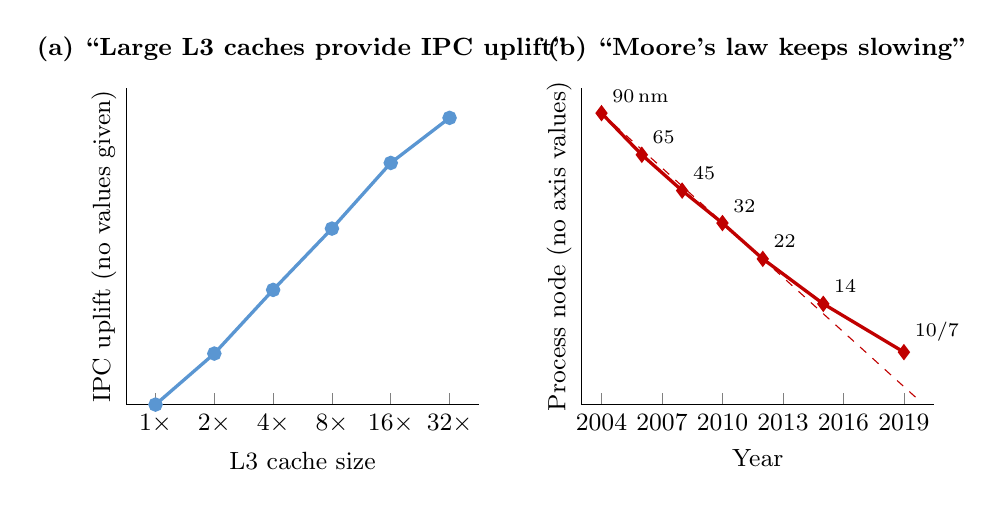
\begin{tikzpicture}
\begin{axis}[
  name=a, width=0.5\textwidth, height=5.6cm,
  title={\small\bfseries (a) ``Large L3 caches provide IPC uplift''},
  xmode=log, log basis x=2, xtick={1,2,4,8,16,32}, xticklabels={1$\times$,2$\times$,4$\times$,8$\times$,16$\times$,32$\times$},
  xticklabel style={font=\small}, xlabel={L3 cache size}, xlabel style={font=\small},
  ymin=0, ymax=8, ytick=\empty, ylabel={IPC uplift (no values given)}, ylabel style={font=\small},
  axis x line*=bottom, axis y line*=left]
\addplot[very thick, color={rgb,255:red,90;green,150;blue,210}, mark=*] coordinates {(1,0) (2,1.29) (4,2.90) (8,4.45) (16,6.11) (32,7.25)};
\end{axis}
\begin{axis}[
  at={(a.east)}, anchor=west, xshift=1.3cm, width=0.5\textwidth, height=5.6cm,
  title={\small\bfseries (b) ``Moore's law keeps slowing''},
  xmin=2003, xmax=2020.5, xtick={2004,2007,2010,2013,2016,2019}, xticklabel style={font=\small, /pgf/number format/1000 sep={}},
  xlabel={Year}, xlabel style={font=\small},
  ymin=-900, ymax=-520, ytick=\empty, ylabel={Process node (no axis values)}, ylabel style={font=\small},
  axis x line*=bottom, axis y line*=left, clip=false]
\addplot[very thick, color={rgb,255:red,192;green,0;blue,0}, mark=diamond*,
  nodes near coords, point meta=explicit symbolic, nodes near coords style={font=\scriptsize, color=black, anchor=south west}]
  coordinates {(2004,-550)[90\,nm] (2006,-600)[65] (2008,-643)[45] (2010,-682)[32] (2012,-725)[22] (2015,-779)[14] (2019,-837)[10/7]};
\addplot[thin, dashed, color={rgb,255:red,192;green,0;blue,0}, domain=2004:2019.6] {-550-21.9*(x-2004)};
\end{axis}
\end{tikzpicture}
\caption[Two of the charts with which AMD's ISSCC~2022 presentation opens, redrawn]{Two of the charts with which AMD's ISSCC~2022 presentation opens, redrawn \cite[slides~5--6]{wuu2022vcache}. (a)~IPC uplift against L3 size on a linear uplift axis. The slide gives no values and names no workloads, so only the shape is shown: each doubling of the L3 up to 16$\times$ adds a similar step, and the last doubling a smaller one. (b)~Process node against year of introduction, with the dashed line continuing the pace of 2004--2012. The slide gives no axis values, so only the positions are reproduced: after 22\,nm each node lies above the earlier trend, that is, it arrived later than that pace would predict. Positions are read from the slide and are approximate.}
\label{fig:isscc-charts}
\end{figure}

Both charts are vendor material, and the first has no stated workloads or values; neither is evidence that every program benefits. Part~\ref{part:case-study} tests the claim against published measurements.

The textbook's miss classes explain why the benefit of a larger cache is uneven. Compulsory misses occur on the first access to a block and no cache size removes them; conflict misses depend on associativity; capacity misses occur because the cache cannot hold everything the program is actively using \cite[sec.~11.3.2]{sarangi2025basic}. Only capacity misses fall as the cache grows, and they fall sharply only when the cache becomes large enough to hold a program's \emph{working set}, the data it reuses over a period of time. \Cref{fig:working-set} sketches the consequence. A program whose working set fits in 32\,MB sees almost no change from a 96\,MB cache; one whose working set is far larger than 96\,MB also sees little change, because most of its data still does not fit; only programs whose working sets lie between the two sizes move from frequent misses to frequent hits. The useful range is set by the ratio of the two capacities, three times, rather than by the extra 64\,MB alone.

\begin{figure}[htbp]
\centering
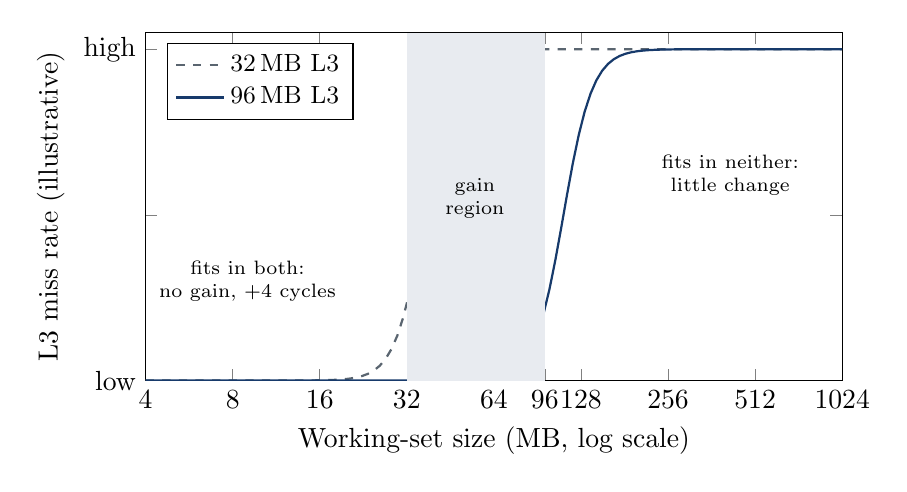
\begin{tikzpicture}
\begin{axis}[
  width=0.86\textwidth, height=6.0cm,
  xmode=log, log basis x=2, xmin=4, xmax=1024,
  xtick={4,8,16,32,64,96,128,256,512,1024}, xticklabels={4,8,16,32,64,96,128,256,512,1024},
  xlabel={Working-set size (MB, log scale)}, ylabel={L3 miss rate (illustrative)},
  ymin=0, ymax=1.05, ytick={0,0.5,1}, yticklabels={low,,high},
  legend pos=north west, legend style={font=\small},
  every axis plot/.append style={thick,samples=120,domain=4:1024}]
\addplot[draftgray,dashed] {1/(1+exp(-6*(ln(x)/ln(2)-5.2)))}; \addlegendentry{32\,MB L3}
\addplot[draftblue] {1/(1+exp(-6*(ln(x)/ln(2)-6.8)))}; \addlegendentry{96\,MB L3}
\fill[draftblue!10] (axis cs:32,0) rectangle (axis cs:96,1.05);
\node[font=\scriptsize,align=center] at (axis cs:55,0.55) {gain\\region};
\node[font=\scriptsize,align=center] at (axis cs:9,0.3) {fits in both:\\no gain, +4 cycles};
\node[font=\scriptsize,align=center] at (axis cs:420,0.62) {fits in neither:\\little change};
\end{axis}
\end{tikzpicture}
\caption[L3 miss rate against working-set size (conceptual)]{Conceptual shape of the L3 miss rate against working-set size for a workload with reuse, for a 32\,MB and a 96\,MB L3. The curves are illustrative, not measured; real transitions are smoother and depend on access pattern, associativity and sharing. They show the three workload classes of \cref{sec:vcache-workloads}.}
\label{fig:working-set}
\end{figure}

\section{Why Expanding Cache in Two Dimensions Became Difficult}
\label{sec:planar-limits}

Growing the L3 in the plane of the compute die meets four related obstacles.

\subsection{Area and yield}
SRAM cells no longer shrink at the rate of logic (\cref{sec:why-cache-capacity}), so a cache of a given capacity occupies a growing share of the die at each new node. AMD lists cost, product flexibility and latency as the resulting barriers to large on-die caches \cite[slide~6]{wuu2022vcache}. Mittal and Vetter add that, if the large caches needed by future workloads were built from SRAM, they could occupy up to 90\% of the chip area \cite[sec.~1]{mittalSurveyTechniquesArchitecting2016}. A larger die yields fewer good dies per wafer (\cref{sec:yield-cost}), so doubling the L3 on a planar CCD would raise the cost of every CCD, including those sold for workloads that do not need the extra cache. It would also make the CCD less flexible as a building block reused across products.

\subsection{Wire length and access latency}
A larger planar cache spreads over a larger area, so the average distance between a core and the cache bank holding its data increases. Longer wires have more resistance and capacitance; their RC delay increases access latency, and the energy needed to charge their capacitance increases dynamic power (\cref{eq:pdyn}). Inside each array the same effect appears at smaller scale: more cells per bit line mean more capacitance to drive, which is why large caches are divided into many small arrays and banks (\cref{sec:sram}).

The effect is measurable even within today's L3. Zen~3 divides its L3 into eight slices, and measurements on a Ryzen~5 5600G show that a core reaches its nearest slice in 40 cycles but needs up to 20 cycles more, 60 in total, for the farthest one (\cref{fig:l3-slices}) \cite{7-cpu.comAMDZen3}. Because consecutive lines are spread across the slices, the average over all eight is what a program sees: $(0+6+1+10+6+13+10+20)/8 \approx 8$ extra cycles for core~0, or about 48 cycles in total, which matches the 47-cycle L3 latency measured on the same processor \cite{7-cpu.comAMDZen3}. Distance on the die is therefore already a visible part of the L3's hit time; a planar L3 three times larger would spread its slices over a larger area and lengthen the farthest paths further.

\begin{figure}[htbp]
\centering
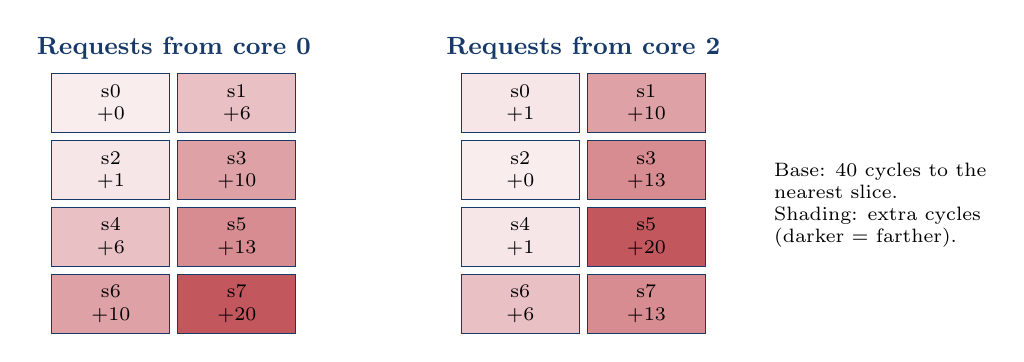
\begin{tikzpicture}[x=1cm,y=1cm,
  sl/.style={draw=draftblue,minimum width=1.5cm,minimum height=0.75cm,font=\scriptsize,align=center},
  lab/.style={font=\small\bfseries,text=draftblue}]
\newcommand{\slice}[4]{\pgfmathsetmacro{\sh}{8+#4*3.4}\node[sl,fill=todored!\sh] at (#1,#2) {#3\\$+#4$};}
\begin{scope}
\node[lab] at (1.0,1.15) {Requests from core 0};
\slice{0.2}{0.45}{s0}{0}  \slice{1.8}{0.45}{s1}{6}
\slice{0.2}{-0.4}{s2}{1}  \slice{1.8}{-0.4}{s3}{10}
\slice{0.2}{-1.25}{s4}{6} \slice{1.8}{-1.25}{s5}{13}
\slice{0.2}{-2.1}{s6}{10} \slice{1.8}{-2.1}{s7}{20}
\end{scope}
\begin{scope}[xshift=5.2cm]
\node[lab] at (1.0,1.15) {Requests from core 2};
\slice{0.2}{0.45}{s0}{1}  \slice{1.8}{0.45}{s1}{10}
\slice{0.2}{-0.4}{s2}{0}  \slice{1.8}{-0.4}{s3}{13}
\slice{0.2}{-1.25}{s4}{1} \slice{1.8}{-1.25}{s5}{20}
\slice{0.2}{-2.1}{s6}{6}  \slice{1.8}{-2.1}{s7}{13}
\end{scope}
\node[font=\scriptsize,align=left,anchor=west] at (8.5,-0.85) {Base: 40 cycles to the\\nearest slice.\\Shading: extra cycles\\(darker = farther).};
\end{tikzpicture}
\caption[Extra latency to each L3 slice of a Zen~3 core (Ryzen~5 5600G)]{Measured extra latency, in cycles beyond the 40-cycle minimum, for a Zen~3 core to reach each of the eight slices of its L3, on a Ryzen~5 5600G \cite{7-cpu.comAMDZen3}. The arrangement of slices follows the source's own table; it is a logical layout, not a floorplan.}
\label{fig:l3-slices}
\end{figure}

 In terms of \cref{eq:amat}, part of the miss-rate gain from a bigger cache is paid back as a longer hit time $t_{\mathrm{LLC}}$. AMD makes the same argument for stacking: compared with spreading a large cache across the plane, 3D integration ``improves effective memory latency'' and ``reduces long datapath and I/O's dynamic powers'' \cite[slide~7]{wuu2022vcache}.

\subsection{Power}
Large SRAM caches consume dynamic power on every read and write and leakage power even when idle (\cref{sec:power}). Mittal and Vetter's survey of DRAM-cache architectures argues that the low density and high leakage power of SRAM make very large SRAM caches infeasible, and that such caches may need expensive cooling, such as liquid cooling, which adds substantial cost and complexity \cite[sec.~1]{mittalSurveyTechniquesArchitecting2016}. This is one reason researchers have explored denser technologies, such as stacked DRAM, for last-level caches.

\subsection{Summary of the planar limits}
Planar expansion therefore trades miss rate against die cost, hit latency and power all at once. The question for the next section is whether a separate cache die can break that coupling.

\section{Side-by-Side Versus Vertically Stacked Cache Dies}
\label{sec:horizontal-vs-vertical}

If extra cache is to be made on its own die, it can be placed either \emph{beside} the compute die in the package or \emph{on top of} it (\cref{fig:horizontal-vs-vertical}). Both are valid chiplet designs; the choice between them is a trade-off.

\begin{figure}[htbp]
\centering
\resizebox{0.6\textwidth}{!}{%
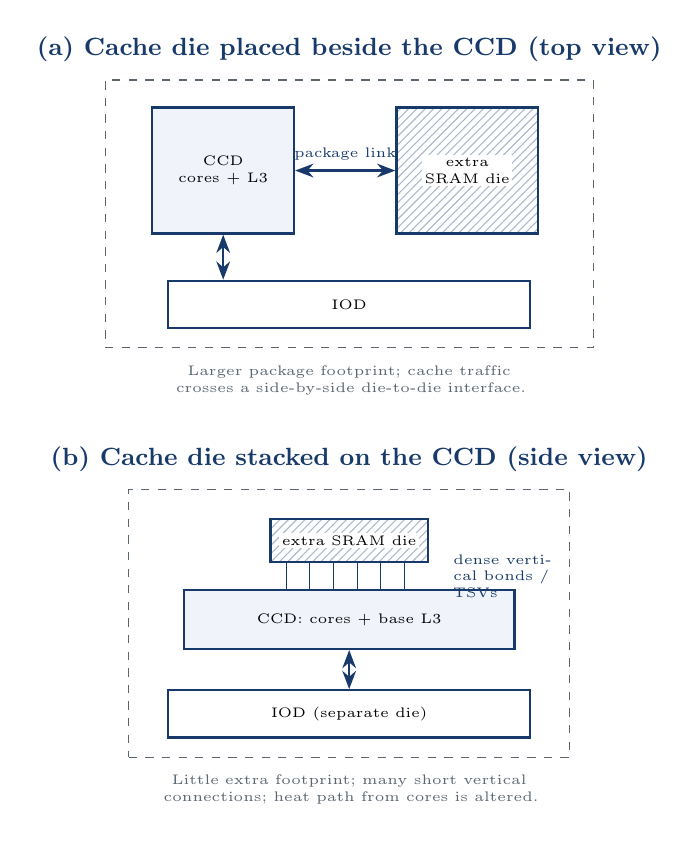
\begin{tikzpicture}[
  die/.style={draw=draftblue,thick,fill=draftlight,align=center,font=\tiny},
  sram/.style={draw=draftblue,thick,fill=white,pattern=north east lines,pattern color=draftblue!35,align=center,font=\tiny},
  lab/.style={font=\small\bfseries,text=draftblue}]
\node[draw=draftgray,dashed,minimum width=6.2cm,minimum height=3.4cm] (pkgA) at (0,0) {};
\node[die,minimum width=1.8cm,minimum height=1.6cm] (ccdA) at (-1.6,0.55) {CCD\\cores + L3};
\node[sram,minimum width=1.8cm,minimum height=1.6cm] (cacheA) at (1.5,0.55) {};
\node[font=\tiny,align=center,fill=white,inner sep=1pt] at (cacheA) {extra\\SRAM die};
\node[die,fill=white,minimum width=4.6cm,minimum height=0.6cm] (iodA) at (0,-1.15) {IOD};
\draw[thick,draftblue,{Stealth}-{Stealth}] (ccdA) -- node[above,font=\tiny]{package link} (cacheA);
\draw[thick,draftblue,{Stealth}-{Stealth}] (ccdA.south) -- (ccdA.south |- iodA.north);
\node[lab,above=0.1cm of pkgA] {(a) Cache die placed beside the CCD (top view)};
\node[font=\tiny,text=draftgray,below=0.1cm of pkgA,text width=6cm,align=center] {Larger package footprint; cache traffic crosses a side-by-side die-to-die interface.};
\begin{scope}[yshift=-5.2cm]
\node[draw=draftgray,dashed,minimum width=5.6cm,minimum height=3.4cm] (pkgB) at (0,0) {};
\node[sram,minimum width=2.0cm,minimum height=0.55cm] (cacheB) at (0,1.05) {};
\node[font=\tiny,fill=white,inner sep=1pt] at (cacheB) {extra SRAM die};
\node[die,minimum width=4.2cm,minimum height=0.75cm] (ccdB) at (0,0.05) {CCD: cores + base L3};
\foreach \x in {-0.8,-0.5,...,0.8}{\draw[draftblue] (\x,0.78) -- (\x,0.43);}
\node[font=\tiny,text=draftblue,anchor=west,text width=1.4cm,align=left] at (1.2,0.6) {dense vertical bonds / TSVs};
\node[die,fill=white,minimum width=4.6cm,minimum height=0.6cm] (iodB) at (0,-1.15) {IOD (separate die)};
\draw[thick,draftblue,{Stealth}-{Stealth}] (ccdB.south) -- (ccdB.south |- iodB.north);
\node[lab,above=0.1cm of pkgB] {(b) Cache die stacked on the CCD (side view)};
\node[font=\tiny,text=draftgray,below=0.1cm of pkgB,text width=5.6cm,align=center] {Little extra footprint; many short vertical connections; heat path from cores is altered.};
\end{scope}
\end{tikzpicture}}
\caption[Two ways to add cache capacity to a compute die]{Two ways to add cache capacity to a compute die. Illustrative arrangements only; not actual AMD package layouts and not to scale.}
\label{fig:horizontal-vs-vertical}
\end{figure}

\subsection{Placing the cache die beside the compute die}
A side-by-side cache die is a perfectly workable chiplet design. It could be connected through the organic substrate or, more densely, through 2.5D packaging (\cref{sec:packaging-options}), but either way it has three costs:
\begin{itemize}
  \item \textbf{Package footprint.} The extra die occupies additional area next to the CCD. This enlarges the \emph{package}, even though it does not enlarge the compute die itself. The distinction between \emph{die area} (one piece of silicon) and \emph{package footprint} (the area of the assembled processor) is important throughout this part.
  \item \textbf{Interconnect.} Every access to the extra cache must cross a die-to-die interface through the package or an interposer. Package-level connections are far coarser than on-die wiring, which limits how many parallel connections---and hence how much bandwidth---the link can offer.
  \item \textbf{Latency and power.} Data must travel between the dies, adding interface circuitry and wire delay to every access to the extra cache, and energy to every bit moved.
\end{itemize}

A side-by-side die does not automatically push the CCD farther from the IOD: the package designer chooses where each die goes, and the cache die could be placed on the far side of the CCD. However, package area is limited, the CCD--IOD links are already routed with care to minimise memory latency \cite{naffziger2020chiplet}, and every additional die competes for the same routing resources. At high signalling rates, longer and more numerous package routes bring RC delay, power, signal-integrity and routing-congestion problems. These can be mitigated with better interconnect design, buffering and packaging technology, so they are engineering costs.

The more important comparison is therefore not the CCD-to-IOD distance but the latency and bandwidth of the path \emph{between the cores and the additional cache}.

AMD's own framing of the choice matches this analysis. Its ISSCC~2022 presentation illustrates a hypothetical processor whose large cache is split off onto a side-by-side chiplet. It states that ``2.5D chiplets can provide product flexibility and reduce cost'' but that ``3D can be even better'', because it improves effective memory latency, reduces long-datapath and I/O dynamic power, and ``fits more transistors within a given package cavity size'' \cite[slide~7]{wuu2022vcache}.

\subsection{Stacking the cache die on the compute die}
Vertical stacking changes the trade-off:
\begin{itemize}
  \item \textbf{Footprint.} The cache die overlaps the CCD's existing footprint, so capacity grows with little additional package area.
  \item \textbf{Interconnect density.} The two dies can be joined by a very large number of short vertical connections, which supports the bandwidth a large cache needs and keeps the added distance small.
  \item \textbf{Thermal design.} The stack can obstruct heat flow from the compute die, depending on which die is on top and what lies above the cores. This is the central new engineering problem (\cref{sec:thermal}).
\end{itemize}

\begin{table}[htbp]
  \centering
  \caption[Qualitative comparison of side-by-side and vertically stacked cache dies]{Qualitative comparison of side-by-side and vertically stacked cache dies.}
  \label{tab:horizontal-vs-vertical}
  \small
  \begin{tabularx}{\textwidth}{@{}>{\raggedright\arraybackslash}p{3.1cm}>{\raggedright\arraybackslash}X>{\raggedright\arraybackslash}X@{}}
    \toprule
    \textbf{Factor} & \textbf{Cache die beside the CCD} & \textbf{Cache die stacked on the CCD} \\
    \midrule
    Package footprint & Larger & More compact \\
    Connections & Side-by-side package or interposer link & Dense vertical bonds and through-silicon vias \\
    Cache access latency & Depends on the interface design & Can benefit from short, dense connections \\
    Cooling & Easier to arrange & More difficult; depends on stack order \\
    Manufacturing & Extra die plus package assembly & Extra die plus bonding, thinning and stacking \\
    \bottomrule
  \end{tabularx}
\end{table}

\Cref{tab:horizontal-vs-vertical} summarises the comparison. The case for vertical stacking is not that side-by-side chiplets cannot work. It is that stacking can add substantial cache capacity without enlarging the package by the same amount, with potentially better interconnect characteristics. The question worth investigating is \emph{when the extra complexity of 3D integration is worth the smaller footprint and denser interconnect}.

\section{Stacked-Die Integration and Hybrid Bonding}
\label{sec:hybrid-bonding}

\subsection{The Zen~3 3D V-Cache stack}
This paper calls the arrangement of the Zen~3 and Zen~4 V-Cache parts, with the cache die on top of the CCD, the \emph{cache-on-top stack}\index{3D V-Cache!cache-on-top stack}; \cref{sec:thermal-evidence} explains why AMD's generation labels are avoided. AMD's Hot Chips~33 presentation describes the Zen~3 stack as a 64\,MB L3 cache die attached to an up-to-eight-core Zen~3 CCD by a direct copper-to-copper bond, with \glspl{tsv} carrying signals and power through the CCD \cite{swaminathanAdvancedPackagingEnabling2021}. AMD's EPYC~7003 documentation states that the L3 cache tiles are stacked on the central L3 portion of the base CCX \cite{amd2022epyc7003}. The ISSCC~2022 presentation describes the three components of the stack and how they are assembled \cite[slides~10--12, 14, 16--17]{wuu2022vcache}:
\begin{itemize}
  \item the Zen~3 CCD, built on TSMC's 7\,nm process with eight cores sharing 32\,MB of L3 in an area of 81\,mm$^2$, with V-Cache support designed in ``from Day~1'';
  \item the extended L3 die (L3D in AMD's slides, which the following paragraphs describe; the cache die elsewhere in this paper), also 7\,nm, carrying 64\,MB of L3 in 41\,mm$^2$, roughly half the CCD area;
  \item structural silicon dies, which provide mechanical support for the thinned CCD and a path for heat from the CPU cores.
\end{itemize}
The CCD is mounted face-down on the package substrate through conventional C4 bumps and connects to the L3D through TSVs. The L3D is mounted face-down on the CCD by hybrid bonding, using TSMC's System on Integrated Chips (SoIC) process with a minimum TSV pitch of 9\,\textmu m, while the structural dies are oxide-bonded beside it. Support silicon brings the stack to the same height as a plain CCD, so server parts with and without V-Cache fit the same package. The cache die sits over the CCD's central L3 region \cite{amd2022epyc7003} and the structural silicon over the cores, so the hottest circuits are covered only by passive silicon. \Cref{fig:vcache-stack} shows the arrangement in cross-section.

\begin{figure}[htbp]
\centering
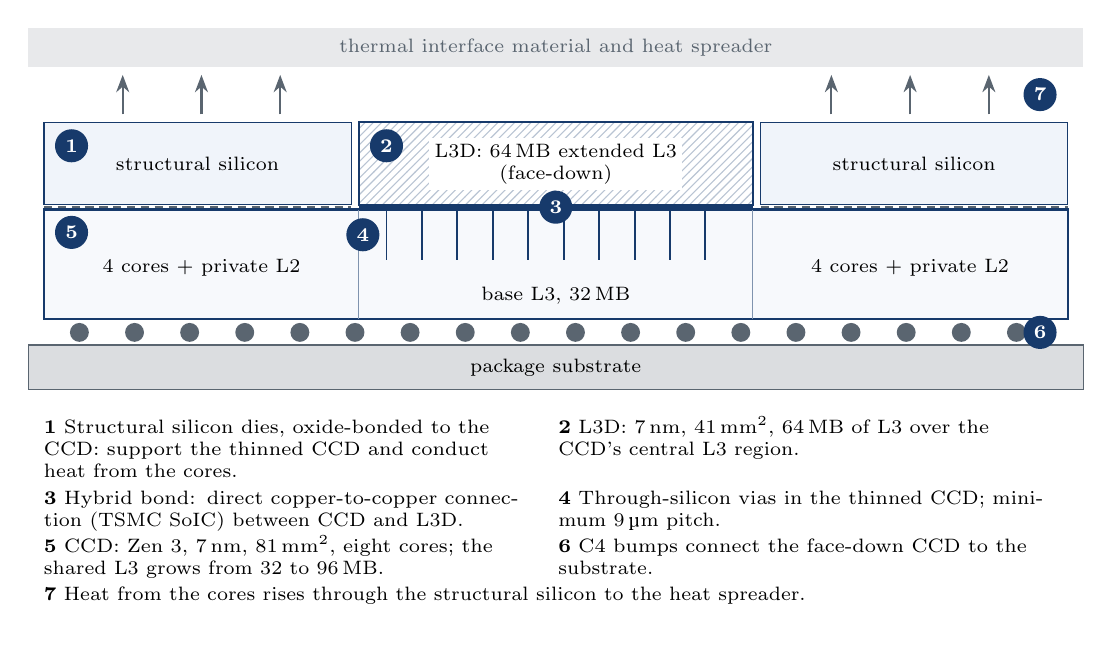
\begin{tikzpicture}[x=1cm,y=1cm,
  mk/.style={circle,fill=draftblue,text=white,font=\scriptsize\bfseries,inner sep=0pt,minimum size=4.2mm},
  lay/.style={font=\scriptsize,align=center}]
\def\W{13.0}\def\Lx{4.0}\def\Rx{9.0}
\fill[draftgray!14] (-0.2,4.75) rectangle (\W+0.2,5.25);
\node[lay,text=draftgray] at (\W/2,5.0) {thermal interface material and heat spreader};
\foreach \x in {1.0,2.0,3.0,10.0,11.0,12.0}{\draw[-{Stealth[length=2.2mm]},draftgray,thick] (\x,4.15) -- (\x,4.65);}
\filldraw[fill=draftlight,draw=draftblue] (0,3.0) rectangle (\Lx-0.1,4.05);
\filldraw[fill=draftlight,draw=draftblue] (\Rx+0.1,3.0) rectangle (\W,4.05);
\fill[pattern=north east lines,pattern color=draftblue!30] (\Lx,3.0) rectangle (\Rx,4.05);
\draw[draftblue,thick] (\Lx,3.0) rectangle (\Rx,4.05);
\node[lay] at ({(\Lx-0.1)/2},3.52) {structural silicon};
\node[lay] at ({(\Rx+0.1+\W)/2},3.52) {structural silicon};
\node[lay,fill=white,inner sep=2pt] at ({(\Lx+\Rx)/2},3.52) {L3D: 64\,MB extended L3\\(face-down)};
\draw[draftblue,line width=1.4pt] (\Lx,2.97) -- (\Rx,2.97);
\draw[draftgray,densely dashed,line width=0.9pt] (0,2.97) -- (\Lx-0.1,2.97) (\Rx+0.1,2.97) -- (\W,2.97);
\filldraw[fill=draftlight!55,draw=draftblue,thick] (0,1.55) rectangle (\W,2.94);
\draw[draftblue!55] (\Lx,1.55) -- (\Lx,2.94) (\Rx,1.55) -- (\Rx,2.94);
\node[lay] at ({\Lx/2},2.2) {4 cores + private L2};
\node[lay] at ({(\Rx+\W)/2},2.2) {4 cores + private L2};
\node[lay] at ({(\Lx+\Rx)/2},1.85) {base L3, 32\,MB};
\foreach \x in {4.35,4.8,...,8.75}{\draw[draftblue,line width=0.7pt] (\x,2.3) -- (\x,2.94);}
\foreach \x in {0.45,1.15,...,12.7}{\fill[draftgray] (\x,1.38) circle (0.12);}
\filldraw[fill=draftgray!22,draw=draftgray] (-0.2,0.65) rectangle (\W+0.2,1.22);
\node[lay] at (\W/2,0.93) {package substrate};
\node[mk] at (0.35,3.75) {1};
\node[mk] at (\Lx+0.35,3.75) {2};
\node[mk] at (6.5,2.97) {3};
\node[mk] at (4.05,2.62) {4};
\node[mk] at (0.35,2.65) {5};
\node[mk] at (12.65,1.38) {6};
\node[mk] at (12.65,4.4) {7};
\node[anchor=north,font=\scriptsize,text width=\W cm] at (\W/2,0.45) {%
\begin{tabular}{@{}p{0.47\linewidth}p{0.47\linewidth}@{}}
\textbf{1} Structural silicon dies, oxide-bonded to the CCD: support the thinned CCD and conduct heat from the cores. &
\textbf{2} L3D: 7\,nm, 41\,mm$^2$, 64\,MB of L3 over the CCD's central L3 region. \\[2pt]
\textbf{3} Hybrid bond: direct copper-to-copper connection (TSMC SoIC) between CCD and L3D. &
\textbf{4} Through-silicon vias in the thinned CCD; minimum 9\,\textmu m pitch. \\[2pt]
\textbf{5} CCD: Zen~3, 7\,nm, 81\,mm$^2$, eight cores; the shared L3 grows from 32 to 96\,MB. &
\textbf{6} C4 bumps connect the face-down CCD to the substrate. \\[2pt]
\multicolumn{2}{@{}p{0.96\linewidth}@{}}{\textbf{7} Heat from the cores rises through the structural silicon to the heat spreader.}
\end{tabular}};
\end{tikzpicture}
\caption[Cross-section of the Zen~3 3D V-Cache stack]{Schematic cross-section of the Zen~3 3D V-Cache stack, drawn from AMD's descriptions \cite[slides~10--12, 14, 16--17]{wuu2022vcache} and \cite{amd2022epyc7003}. Not to scale; layer thicknesses and the number of TSVs are illustrative.}
\label{fig:vcache-stack}
\end{figure}

\subsection{Hybrid bonding versus micro-bumps}
Earlier 3D stacking typically joined dies with solder \glspl{micro-bump}\index{micro-bump}. \Gls{hybrid-bonding} instead bonds aligned copper pads and surrounding dielectric directly. AMD reports, from its internal engineering analysis \cite{swaminathanAdvancedPackagingEnabling2021}:\index{hybrid bonding}
\begin{itemize}
  \item a hybrid-bond pitch of 9\,\textmu m, compared with 50 to 36\,\textmu m for micro-bump 3D;
  \item more than 15$\times$ the interconnect density of micro-bump 3D;
  \item more than 3$\times$ better interconnect power efficiency than micro-bump 3D;
  \item lower TSV capacitance and inductance, which benefits signal and power delivery.
\end{itemize}
AMD's EPYC~7003 documentation similarly claims over 200$\times$ the interconnect density of 2D packaging and over 15$\times$ that of solder-bump 3D \cite{amd2022epyc7003}. These are AMD's own comparisons and should be read as engineering claims.

Interconnect density matters architecturally for three reasons. First, \emph{bandwidth}: the number of parallel connections between two dies limits how much data can cross between them per cycle, and a large L3 serving eight cores needs very wide paths; AMD's stack delivers, by AMD's figure, more than 2\,TB/s \cite[slide~20]{wuu2022vcache}. Second, \emph{latency}: vertical connections a few micrometres long add very little wire delay, which helps explain why the extra 64\,MB costs only four cycles. Third, \emph{energy}: short, low-capacitance connections cost less energy per bit (\cref{eq:pdyn}), which AMD quantifies as more than 3$\times$ better than micro-bump stacking \cite[slide~15]{wuu2022vcache}. The low parasitics of hybrid bonding also let AMD use a simple digital signal interface between the dies rather than the serialising transceivers needed by package-level chiplet links \cite[slide~26]{wuu2022vcache}. These are exactly the costs that \cref{sec:horizontal-vs-vertical} identified for a side-by-side cache die.

\subsection{What a finer pitch buys}
\label{sec:density-example}
Pitch is the distance between the centres of neighbouring connections. If pads are laid out on a square grid of pitch $p$, a square millimetre holds
\begin{equation}
  n \;=\; \left(\frac{1000\,\text{\textmu m}}{p}\right)^{2}
  \label{eq:pad-density}
\end{equation}
connections. At the 36\,\textmu m micro-bump pitch quoted by AMD this gives $(1000/36)^2 \approx 772$ connections per mm$^2$; at the 9\,\textmu m hybrid-bond pitch it gives $(1000/9)^2 \approx 12\,346$, sixteen times as many, which is consistent with AMD's claim of more than 15$\times$ the density \cite{swaminathanAdvancedPackagingEnabling2021}. Against C4 bumps at AMD's 150\,\textmu m limit \cite[slide~13]{lambertHeterogenousIntegrationHigh2025}, about 44 per mm$^2$, the hybrid bond offers roughly 280 times as many, the same order as AMD's ``over 200$\times$'' comparison with 2D packaging \cite{amd2022epyc7003}. Because density grows with the square of the pitch reduction, each halving of the pitch gives four times as many connections (\cref{fig:interconnect-density}).

The architectural meaning becomes clear from the area involved. Suppose, for illustration only, that a 1\,mm$^2$ strip of the CCD were given over entirely to signal connections. At the hybrid-bond pitch it could carry about twelve thousand signals; a 32-byte (256-bit) interface for each of eight cores in both directions needs $8 \times 256 \times 2 = 4096$ data wires, a third of that budget before clocks, control and spares. At the micro-bump pitch the same interface would need more than 5\,mm$^2$, and at the C4 pitch more than 90\,mm$^2$, larger than the whole CCD. This is a model calculation, not AMD's layout, but it shows that such an interface is impractical at C4 pitch and would cost several mm$^2$ at micro-bump or 2.5D pitch, whereas hybrid bonding fits it in a fraction of a square millimetre. Package-level chiplet links, which use C4-class bumps on an organic substrate, must instead serialise data over a few fast lanes (\cref{sec:d2d}).

\begin{figure}[htbp]
\centering
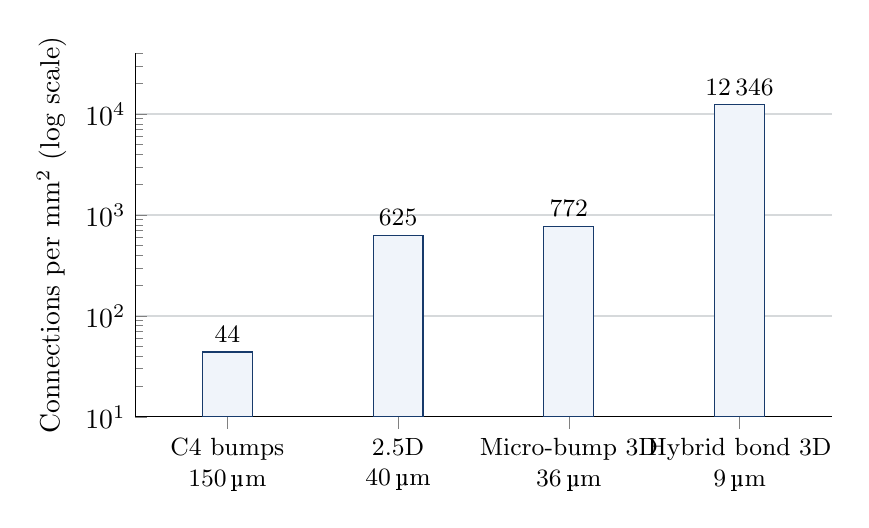
\begin{tikzpicture}
\begin{axis}[
  ybar, bar width=18pt, width=0.86\textwidth, height=6.2cm,
  ymode=log, log origin=infty, ymin=10, ymax=40000,
  ylabel={Connections per mm$^2$ (log scale)},
  symbolic x coords={C4,2.5D,Micro-bump,Hybrid bond},
  xtick=data,
  xticklabels={{C4 bumps\\150\,\textmu m},{2.5D\\40\,\textmu m},{Micro-bump 3D\\36\,\textmu m},{Hybrid bond 3D\\9\,\textmu m}},
  xticklabel style={align=center,font=\small},
  nodes near coords, nodes near coords style={font=\small},
  point meta=explicit symbolic,
  ymajorgrids, grid style={draftgray!25}, axis x line*=bottom, axis y line*=left,
  enlarge x limits=0.18]
\addplot[fill=draftlight,draw=draftblue] coordinates {(C4,44)[44] (2.5D,625)[625] (Micro-bump,772)[772] (Hybrid bond,12346)[12\,346]};
\end{axis}
\end{tikzpicture}
\caption[Connections per mm$^2$ at each interconnect pitch]{Connections per square millimetre for a square grid of pads at each pitch, $(1000/p)^2$ for a pitch $p$ in micrometres. Pitches are AMD's stated limits for C4 bumps and 2.5D \cite[slide~13]{lambertHeterogenousIntegrationHigh2025}, the finest micro-bump pitch AMD quotes, and the 9\,\textmu m hybrid-bond pitch \cite{swaminathanAdvancedPackagingEnabling2021}. Real layouts are not full square grids, so the values are upper bounds for comparison only.}
\label{fig:interconnect-density}
\end{figure}

\subsection{How a hybrid bond is made}
\label{sec:bond-process}
Hybrid bonding joins two surfaces that each contain both oxide and copper pads. The oxide surfaces bond first; the copper pads start slightly recessed, and during the anneal the copper diffuses across the interface and joins them \cite[slide~9]{alam2ndGeneration3D2024}. No solder is involved, and solder is what limits the pitch of micro-bumps (\cref{sec:hybrid-bonding}), which is why the pitch can be so much finer.

\Cref{fig:bond-interface} shows one connection. In the Zen~3 stack, the copper pads on each die are called bond-pad metal (BPM). On the CCD, the BPM sits on the end of a TSV; on the L3D, a bond-pad via (BPV) connects the BPM to the die's top copper layer, M13 \cite[slide~16]{wuu2022vcache}. The L3D has thirteen copper layers and one aluminium layer \cite[slide~11]{wuu2022vcache}. For Zen~4, AMD changed this detail: the stack became explicitly face-to-back, with a 7\,nm cache die on a 5\,nm CCD, and the BPV lands on the top aluminium pad instead of the top copper layer \cite[slides~11--12]{alam2ndGeneration3D2024}. The process is TSMC's SoIC \cite[slide~16]{wuu2022vcache}.

\begin{figure}[htbp]
\centering
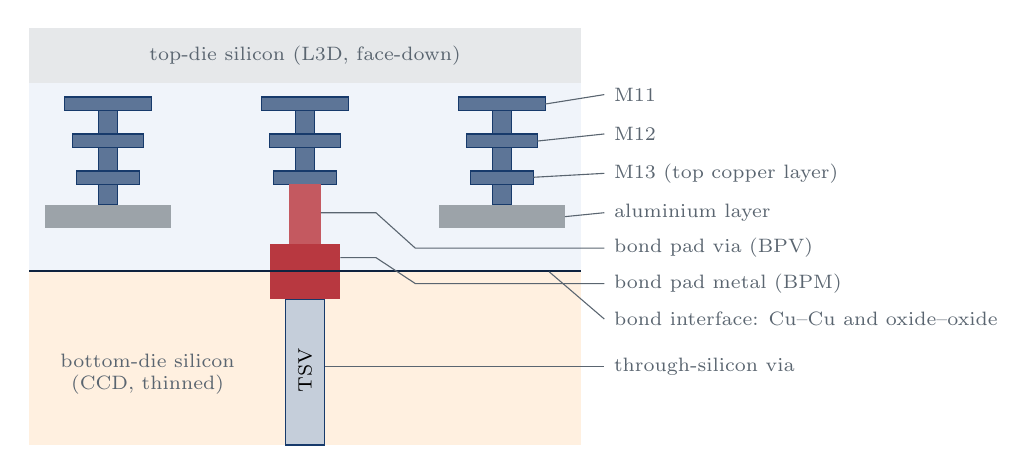
\begin{tikzpicture}[x=1cm,y=1cm,
  met/.style={fill=draftblue!70,draw=draftblue},
  lab/.style={font=\scriptsize,anchor=west},
  callout/.style={draftgray,thin}]
\fill[draftlight] (0,2.2) rectangle (7,4.6);
\fill[draftgray!15] (0,4.6) rectangle (7,5.3);
\node[font=\scriptsize,text=draftgray] at (3.5,4.95) {top-die silicon (L3D, face-down)};
\foreach \x in {1.0,3.5,6.0}{
  \fill[met] (\x-0.55,4.25) rectangle (\x+0.55,4.42); % M11
  \fill[met] (\x-0.12,3.95) rectangle (\x+0.12,4.25);
  \fill[met] (\x-0.45,3.78) rectangle (\x+0.45,3.95); % M12
  \fill[met] (\x-0.12,3.48) rectangle (\x+0.12,3.78);
  \fill[met] (\x-0.4,3.31) rectangle (\x+0.4,3.48);   % M13
}
\fill[draftgray!60] (0.2,2.75) rectangle (1.8,3.05);
\fill[draftgray!60] (5.2,2.75) rectangle (6.8,3.05);
\foreach \x in {1.0,6.0}{\fill[met] (\x-0.12,3.05) rectangle (\x+0.12,3.31);}
\fill[todored!75] (3.3,2.55) rectangle (3.7,3.31);
\fill[todored!90] (3.05,2.2) rectangle (3.95,2.55);
\draw[draftblue!60!black,line width=1.3pt] (0,2.2) -- (7,2.2);
\fill[orange!12] (0,0) rectangle (7,2.2);
\fill[todored!90] (3.05,1.85) rectangle (3.95,2.2);
\fill[draftblue!25,draw=draftblue] (3.25,0) rectangle (3.75,1.85);
\node[font=\scriptsize,rotate=90] at (3.5,0.95) {TSV};
\node[font=\scriptsize,text=draftgray,align=center] at (1.5,0.9) {bottom-die silicon\\(CCD, thinned)};
\draw[callout] (6.55,4.33) -- (7.3,4.45) node[lab]{M11};
\draw[callout] (6.45,3.86) -- (7.3,3.95) node[lab]{M12};
\draw[callout] (6.4,3.4) -- (7.3,3.45) node[lab]{M13 (top copper layer)};
\draw[callout] (6.8,2.9) -- (7.3,2.95) node[lab]{aluminium layer};
\draw[callout] (3.7,2.95) -- (4.4,2.95) -- (4.9,2.5) -- (7.3,2.5) node[lab]{bond pad via (BPV)};
\draw[callout] (3.95,2.38) -- (4.4,2.38) -- (4.9,2.05) -- (7.3,2.05) node[lab]{bond pad metal (BPM)};
\draw[callout] (6.6,2.2) -- (7.3,1.6) node[lab]{bond interface: Cu--Cu and oxide--oxide};
\draw[callout] (3.75,1.0) -- (7.3,1.0) node[lab]{through-silicon via};
\end{tikzpicture}
\caption[One hybrid-bond connection in the Zen~3 stack]{Schematic of one hybrid-bond connection in the Zen~3 stack, redrawn from AMD's description \cite[slide~16]{wuu2022vcache}. Copper bond-pad metal (BPM) on the two dies is bonded directly; on the top die a bond-pad via (BPV) connects the pad to the top copper layer (M13), and on the bottom die the pad lands on a TSV. In the Zen~4 stack the BPV lands on the top aluminium pad instead \cite[slides~11--12]{alam2ndGeneration3D2024}. Not to scale.}
\label{fig:bond-interface}
\end{figure}

\section{Cache Access, Latency, Bandwidth and Hierarchy}
\label{sec:vcache-access}

With the cache die, the L3 of a Zen~3 CCD grows from 32\,MB to 96\,MB, shared by up to eight cores \cite{wuu2022vcache,amd2022epyc7003}; an EPYC~7003 processor with eight such CCDs carries up to 768\,MB of L3 \cite{amd2022epyc7003}. AMD reports more than 2\,TB/s of bandwidth for the V-Cache \cite{wuu2022vcache}. The extra capacity remains part of the same L3 level, so the cache hierarchy above it (private L1 and L2 per core) is unchanged \cite{amd2022epyc7003}.

AMD's presentation gives the cost of the extra capacity in latency: the 96\,MB L3 remains 16-way set associative with a 32\,B/cycle interface to each core, delivers more than 2\,TB/s of L3 bandwidth, and adds \emph{four cycles} of latency \cite[slide~20]{wuu2022vcache}. Independent measurements agree: Chips and Cheese measured roughly three to four extra cycles of L3 latency on Milan-X compared with Milan \cite{cozmaDeepDivingZen2022}, about four extra cycles on the V-Cache CCD of the Zen~4 Ryzen~9 7950X3D \cite{lamAMDs7950X3DZen2023}, and the same four cycles on the Zen~5 Ryzen~7 9800X3D, whose cache die sits below the CCD \cite{cozmaAMDs9800X3D2nd2024}. AMD's bandwidth figure is a peak capability: on Milan-X, single-thread L3 bandwidth measured about 25\% more bytes per cycle than Milan rather than the doubling AMD had announced \cite{cozmaDeepDivingZen2022}. Each die's portion of the L3 has its own data, tag and LRU arrays, so a tag lookup does not have to cross between dies before the data array is accessed \cite[slide~20]{wuu2022vcache}.

\Cref{eq:amat} shows how to judge this trade-off. For an access that has already missed in L2, the extra capacity changes the average cost by approximately
\begin{equation}
  \Delta T \;\approx\; \Delta t_{\mathrm{L3}} \;-\; \Delta m_{\mathrm{L3}} \cdot t_{\mathrm{mem}},
  \label{eq:vcache-tradeoff}
\end{equation}
where $\Delta t_{\mathrm{L3}} = 4$ cycles is the added hit latency, $\Delta m_{\mathrm{L3}}$ the reduction in the L3 miss rate and $t_{\mathrm{mem}}$ the main-memory latency in cycles. The textbook puts the stall for a miss that goes to main memory at 100--300 cycles \cite[sec.~12.4.8]{sarangi2025basic}. Over that range, the larger L3 pays off once it removes more than about $4/300 \approx 1.3$ to $4/100 = 4$ percentage points of L3 misses. A workload whose working set already fits in 32\,MB gains nothing and pays the four cycles on every L3 hit; a workload whose working set lies between 32\,MB and 96\,MB can gain substantially.

\subsection{Applying the trade-off to a measured workload}
\label{sec:tradeoff-example}
Lam's fixed-frequency measurements of the Ryzen~9 7950X3D give enough data to apply \cref{eq:vcache-tradeoff} to a real program \cite{lamAMDs7950X3DZen2023}. For libx264 video encoding, the plain CCD had 1.48 L3 misses per thousand instructions (MPKI). Lam's charts give an L3 hit rate of 61.55\% and an IPC of 1.36 on the plain CCD, against 71.86\% and 1.43 on the V-Cache CCD. (The article's text gives the second hit rate as 72.8\%, but its chart and its stated 16.75\% improvement both correspond to 71.86\%, which is used here.)
\begin{enumerate}
  \item \textbf{L3 accesses.} If 38.45\% of L3 accesses miss and this gives 1.48 misses per thousand instructions, the program makes $1.48 / 0.3845 \approx 3.85$ L3 accesses per thousand instructions.
  \item \textbf{Misses removed.} With V-Cache, $3.85 \times 0.2814 \approx 1.08$ of those accesses still miss, so about $1.48 - 1.08 = 0.40$ misses per thousand instructions are removed.
  \item \textbf{Cycles saved.} At the textbook's 100--300 cycles per memory access \cite[sec.~12.4.8]{sarangi2025basic}, that saves $0.40 \times (100\text{ to }300) \approx 40$ to 120 cycles per thousand instructions.
  \item \textbf{Cycles added.} Every L3 access pays four more cycles: $3.85 \times 4 \approx 15$ cycles per thousand instructions.
  \item \textbf{Net effect.} About 25 to 105 cycles saved per thousand instructions.
\end{enumerate}
At an IPC of 1.36, a thousand instructions take $1000/1.36 \approx 735$ cycles, so the model predicts 3--14\% fewer cycles. The measurement lies inside that range: at an IPC of 1.43 the same work takes about 699 cycles, 4.9\% fewer (an IPC gain of 5.1\% from the rounded chart values; Lam states 4.9\%). \Cref{fig:libx264-waterfall} shows how this change divides between the two effects.

\begin{figure}[htbp]
\centering
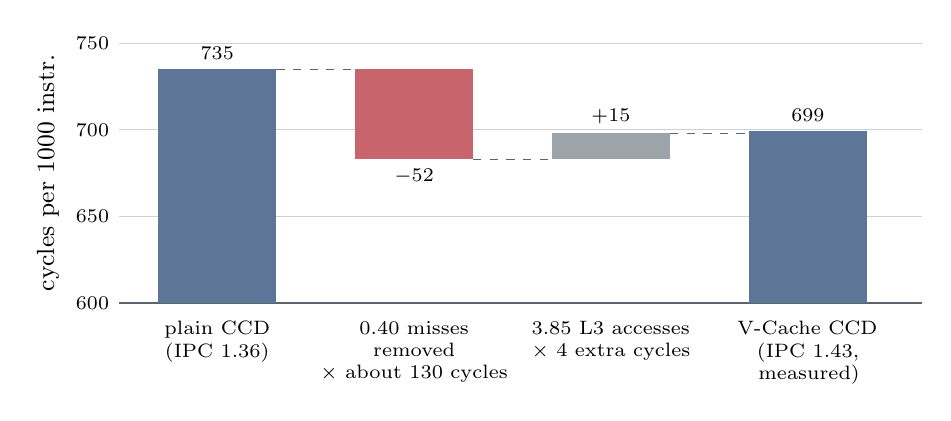
\begin{tikzpicture}[x=1cm,y=0.022cm,
  lab/.style={font=\scriptsize,align=center,anchor=north,text width=2.4cm}]
\def\base{600}
\foreach \v in {600,650,700,750} {\draw[draftgray!30] (0,\v) -- (10.2,\v); \node[font=\scriptsize,anchor=east] at (0,\v) {\v};}
\draw[draftgray] (0,\base) -- (10.2,\base);
\node[font=\small,rotate=90] at (-0.9,675) {cycles per 1000 instr.};
\fill[draftblue!70] (0.5,\base) rectangle (2.0,735);
\node[font=\scriptsize,anchor=south] at (1.25,735) {735};
\fill[todored!70] (3.0,683) rectangle (4.5,735);
\node[font=\scriptsize,anchor=north] at (3.75,683) {$-52$};
\fill[draftgray!60] (5.5,683) rectangle (7.0,698);
\node[font=\scriptsize,anchor=south] at (6.25,698) {$+15$};
\fill[draftblue!70] (8.0,\base) rectangle (9.5,699);
\node[font=\scriptsize,anchor=south] at (8.75,699) {699};
\draw[draftgray,dashed] (2.0,735) -- (3.0,735) (4.5,683) -- (5.5,683) (7.0,698) -- (8.0,698);
\node[lab] at (1.25,595) {plain CCD\\(IPC 1.36)};
\node[lab] at (3.75,595) {0.40 misses removed\\$\times$ about 130 cycles};
\node[lab] at (6.25,595) {3.85 L3 accesses\\$\times$ 4 extra cycles};
\node[lab] at (8.75,595) {V-Cache CCD\\(IPC 1.43, measured)};
\end{tikzpicture}
\caption[The libx264 calculation as a sequence]{The libx264 calculation of \cref{sec:tradeoff-example} as a sequence: starting from the plain CCD's 735 cycles per thousand instructions, the misses removed by the larger L3 save about 52 cycles and the four extra cycles on every L3 access cost about 15, leaving about 698 against the 699 implied by the measured IPC. The stall of about 130 cycles per removed miss is itself inferred from the measurement, so the chart shows how the measured change divides between the two effects rather than predicting it independently. Both CCDs fixed at 4.2\,GHz; data from Lam \cite{lamAMDs7950X3DZen2023}. The vertical axis starts at 600.}
\label{fig:libx264-waterfall}
\end{figure}


The measurement can also be turned around. The observed saving of about 36 cycles per thousand instructions, plus the 15 cycles of added L3 latency, implies that each removed miss saved about $(36 + 15)/0.40 \approx 130$ cycles. That is at the low end of the textbook's 100--300-cycle range, which is expected if an out-of-order core overlaps some memory misses with other work (\cref{sec:mlp}): removing a miss then saves less than its full latency.

The 130 cycles should be read as an \emph{apparent} saving per counted miss, for two reasons. First, Lam counts L3 accesses from the L3's side, including speculative accesses and without separating prefetches from demand requests \cite{lamAMDs7950X3DZen2023}. A removed prefetch miss need not have stalled the core at all, so prefetching is a second explanation, besides overlap, for a saving below the full latency. Second, the calculation rests on four assumptions besides the textbook's latency range. They are that all of the IPC change comes from L3 misses and L3 latency; that every L3 access pays all four extra cycles; that both CCDs make the same number of L3 accesses per thousand instructions; and that the counted misses are the ones the core waits for. The third can be checked on the one workload for which Lam states both MPKIs, the flight simulator DCS discussed next. Its 0.35 misses at a 10.9\% miss rate imply 3.2 L3 accesses per thousand instructions on the plain CCD, but 0.28 at 7.6\% imply 3.7 on the V-Cache CCD, about 15\% more; the method would have predicted 0.24 MPKI with V-Cache rather than the 0.28 measured. The 130 cycles is therefore an estimate with an uncertainty of this order, not a measured stall.

The same arithmetic explains the small loss Lam observed in a flight simulator with only 0.35 MPKI, falling to 0.28 with V-Cache \cite{lamAMDs7950X3DZen2023}. Removing 0.07 misses per thousand instructions saves at most 7--21 cycles, which can be outweighed by four extra cycles on each of its L3 hits. The model's range brackets the measurement, and both agree with the miss-class argument of \cref{sec:why-cache-capacity}.

\subsection{Inside the cache interface}
\label{sec:cache-interface}
AMD's ISSCC presentation describes how the stacked half of the L3 is organised and connected, and the details explain why the latency cost is so small (\cref{fig:vcache-floorplan}).

\textbf{Where the connections are.} On the CCD, two columns of signal TSVs run along either side of the central 32\,MB L3, between the L3 and the two rows of four cores \cite[slide~10]{wuu2022vcache}. The L3D has matching ``CCD signal interface'' columns directly above them \cite[slide~11]{wuu2022vcache}. The L3 already sits at the centre of the CCD, with every core's 32\,B/cycle interface entering it from the side \cite[slides~19, 21]{wuu2022vcache}, so the stacked cache is reached through the same central region rather than through a new path across the die. AMD states that support for V-Cache was integrated in the CCD ``from Day~1'' \cite[slide~10]{wuu2022vcache}: the TSV columns occupy CCD area in every Zen~3 CCD, including those sold without a cache die.

\textbf{How the stacked arrays are organised.} The L3D holds 512 data macros and 1088 tag and LRU macros, so each portion of the L3 keeps its own tags and the lookup does not cross between dies. \Cref{app:l3d-organisation} works through the macro counts, the cost of the tags (about 10\% of the data capacity) and the set count of the combined 96\,MB cache \cite[slides~20, 25]{wuu2022vcache}.

\textbf{Checking the bandwidth claim.} Each core has a 32\,B/cycle interface to the L3, and AMD describes the stacked connection as a 32\,B/cycle bidirectional bus \cite[slides~20--21]{wuu2022vcache}. If all eight cores transfer 32 bytes per cycle in each direction at an assumed L3 clock of 4\,GHz, the total is
\[
  8 \times 32\,\text{B} \times 2 \times 4 \times 10^{9}\,\text{s}^{-1} \;\approx\; 2.0\,\text{TB/s},
\]
consistent with AMD's ``more than 2\,TB/s'' \cite[slide~20]{wuu2022vcache}. The figure is therefore an aggregate peak across all cores and both directions, and no independent test has reached it. Chips and Cheese's single-thread measurement on Milan-X found about 25\% more bytes per cycle than on Milan, with an estimated clock, but its test of one whole CCD found Milan-X about 12.5\% \emph{lower} in bytes per cycle \cite{cozmaDeepDivingZen2022}. Lam's all-core test on the 7950X3D, at a fixed 4.2\,GHz, found the V-Cache CCD averaging 18.45 bytes per cycle per core, slightly below the plain CCD \cite{lamAMDs7950X3DZen2023}. For eight cores that is about $8 \times 18.45 \times 4.2 \times 10^{9} \approx 0.62$\,TB/s at the 4.2\,GHz of that test, or about 0.71\,TB/s at the 4.8\,GHz the V-Cache CCD sustained at stock clocks, consistent with the 702\,GB/s of Lam's multithreaded test. The 2\,TB/s is therefore AMD's peak for the interface, not a bandwidth that programs have been shown to obtain.

\textbf{A simple signal interface.} Because hybrid-bond connections have low parasitics, each signal crosses between the dies through an ordinary digital path: a flip-flop and driver on one side, the TSV, electrostatic-discharge protection and an isolation stage on the other, and a receiving flip-flop \cite[slide~26]{wuu2022vcache}. No serialiser, equaliser or separate link clock is needed. By contrast, the CCD-to-IOD link of \cref{sec:d2d} is a serial interface with a round trip of 13 fabric clocks. This difference probably explains much of why a stacked cache can add only four cycles while a die-to-die hop through the package costs several nanoseconds (under 9\,ns for the round trip in Rome \cite{naffziger2020chiplet}), against about 1\,ns for four cycles at 4\,GHz.

\begin{figure}[htbp]
\centering
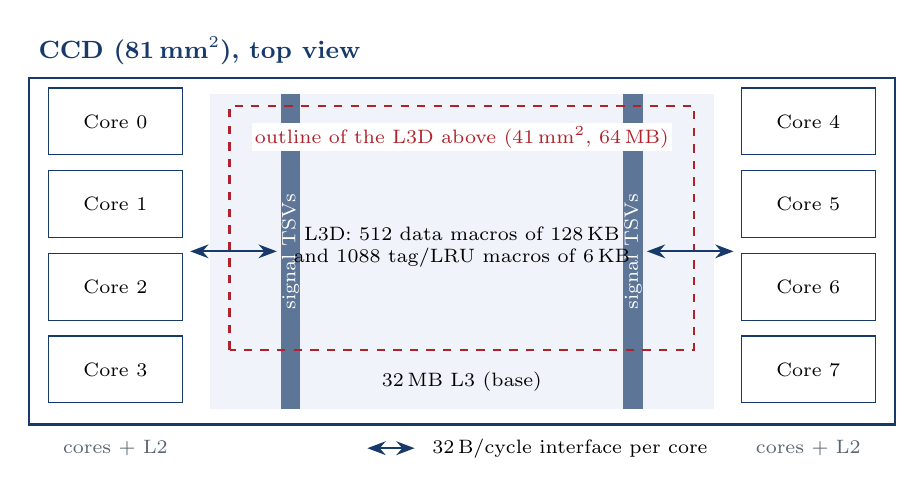
\begin{tikzpicture}[x=1cm,y=1cm,
  core/.style={draw=draftblue,fill=white,font=\scriptsize,minimum width=1.7cm,minimum height=0.85cm},
  tsv/.style={fill=draftblue!70},
  lab/.style={font=\scriptsize,align=center}]
\draw[draftblue,thick] (0,0) rectangle (11,4.4);
\node[font=\small\bfseries,text=draftblue,anchor=south west] at (0,4.45) {CCD (81\,mm$^2$), top view};
\foreach \i in {0,1,2,3}{
  \node[core] at (1.1,3.85-\i*1.05) {Core \i};
  \node[core] at (9.9,3.85-\i*1.05) {Core \the\numexpr\i+4\relax};}
\node[lab,text=draftgray] at (1.1,-0.3) {cores + L2};
\node[lab,text=draftgray] at (9.9,-0.3) {cores + L2};
\fill[draftlight] (2.3,0.2) rectangle (8.7,4.2);
\node[lab] at (5.5,0.55) {32\,MB L3 (base)};
\fill[tsv] (3.2,0.2) rectangle (3.45,4.2);
\fill[tsv] (7.55,0.2) rectangle (7.8,4.2);
\node[lab,rotate=90,text=white] at (3.325,2.2) {signal TSVs};
\node[lab,rotate=90,text=white] at (7.675,2.2) {signal TSVs};
\draw[todored,thick,dashed] (2.55,0.95) rectangle (8.45,4.05);
\node[lab,text=todored,fill=white,inner sep=1pt] at (5.5,3.65) {outline of the L3D above (41\,mm$^2$, 64\,MB)};
\node[lab,align=center] at (5.5,2.25) {L3D: 512 data macros of 128\,KB\\and 1088 tag/LRU macros of 6\,KB};
\draw[{Stealth}-{Stealth},thick,draftblue] (2.05,2.2) -- (3.15,2.2);
\draw[{Stealth}-{Stealth},thick,draftblue] (7.85,2.2) -- (8.95,2.2);
\draw[{Stealth}-{Stealth},thick,draftblue] (4.3,-0.3) -- (4.9,-0.3); \node[lab,anchor=west] at (5.0,-0.3) {32\,B/cycle interface per core};
\end{tikzpicture}
\caption[Top view of how the L3D connects to the CCD, redrawn from AMD's descriptions]{Top view of how the L3D connects to the CCD, redrawn from AMD's descriptions \cite[slides~10--11, 19--21, 25]{wuu2022vcache}. Two columns of signal TSVs run along the CCD's central L3, and matching interface columns on the L3D lie directly above them. Each core reaches the L3 over a 32\,B/cycle interface. Positions and sizes are schematic; the L3D outline is drawn only approximately over the L3 region.}
\label{fig:vcache-floorplan}
\end{figure}

The L3 remains private to each CCD, so a thread running on one CCD does not benefit from another CCD's stacked cache.

\section{Thermal Management, Power Delivery and Manufacturing Complexity}
\label{sec:thermal}

Stacking changes the heat path described in \cref{sec:power}: heat from the cores must now pass through additional silicon and bonding layers before it reaches the heat spreader. The cache-on-top design limits the penalty by placing the cache die over the CCD's central L3 region \cite{amd2022epyc7003} and covering the cores only with structural silicon, whose stated purposes include ``thermal dissipation for CPU cores'' \cite[slide~12]{wuu2022vcache}. AMD also credits hybrid bonding with ``superior thermal conductance'' compared with micro-bump stacking \cite[slide~15]{wuu2022vcache}, although this is an AMD claim based on internal simulation. Earlier academic work gives a sense of scale. Black \emph{et al.} simulated an extra 8\,MB of SRAM stacked on a Core~2~Duo-class processor: the peak temperature rose from 88.35\,\textdegree C to 92.85\,\textdegree C, whereas a 32\,MB stacked DRAM cache raised it only to 88.43\,\textdegree C, because SRAM has the higher power density \cite{blackStacking3DMicroarchitecture2006}. These are 2006 simulations of an older stacking technology and are indicative only.

\Cref{eq:thermal} gives a way to reason about these numbers. Treat a core's hot spot as one grid point with power $P$ and an effective thermal resistance $R$ to ambient, so that its temperature rise is $\Delta T = RP$. Any layer added above the core adds its own resistance in series, raising $R$ and therefore $\Delta T$ for the same power. As an illustration with assumed values only: a hot spot that runs 60\,K above ambient through its original heat path runs 66\,K above ambient if the added layer raises $R$ by 10\%. Because leakage rises with temperature, the extra 6\,K also raises $P$ slightly, and the feedback loop of \cref{sec:power} increases the final temperature further. The designer then has two choices: accept the higher temperature, or lower voltage and frequency until $P$ falls enough to compensate. The measured clock and voltage limits of the cache-on-top parts (\cref{sec:thermal-evidence}) are consistent with the second choice, although the sources attribute them at least partly to the stacked cache's lower voltage tolerance rather than to temperature alone \cite{lamAMDs7950X3DZen2023}. Black \emph{et al.}'s simulations show the same effect in reverse: the stacked SRAM die adds both its own power and a layer, so its 4.5\,K rise is much larger than that of a lower-power stacked DRAM \cite{blackStacking3DMicroarchitecture2006}.

\Cref{fig:mindmap-stack-costs} collects the costs of stacking discussed in this section and AMD's responses to them.

\mapfigure{%
\node[mmroot] (r) {What stacking costs, and AMD's answers};
\node[mmbox,mmlevel1,fill=mmF4AAA2] (b0) at (0.00,3.60) {Heat path};
\draw[mmbig] (r) -- (b0);
\node[mmlevel2,mmbox,fill=mmCFE7E1] (b0c0) at (-3.05,5.35) {Extra layers raise $R$};
\draw[mmsmall] (b0.north) to[out=90,in=-90] (b0c0.south);
\node[mmlevel2,mmbox,fill=mmCFE7E1] (b0c1) at (0.00,5.35) {Leakage feedback};
\draw[mmsmall] (b0.north) to[out=90,in=-90] (b0c1.south);
\node[mmlevel2,mmbox,fill=mmCFE7E1] (b0c2) at (3.05,5.35) {Hot spot: $\Delta T = RP$};
\draw[mmsmall] (b0.north) to[out=90,in=-90] (b0c2.south);
\node[mmbox,mmlevel1,fill=mmF9D7AF] (b1) at (4.47,1.36) {Voltage and clock};
\draw[mmbig] (r) -- (b1);
\node[mmlevel2,mmbox,fill=mmDCCFF6] (b1c0) at (8.07,2.81) {1.2\,V limit (7800X3D)};
\draw[mmsmall] (b1.east) to[out=0,in=180] (b1c0.west);
\node[mmlevel2,mmbox,fill=mmDCCFF6] (b1c1) at (8.07,1.36) {4.8 against 5.15\,GHz (7950X3D)};
\draw[mmsmall] (b1.east) to[out=0,in=180] (b1c1.west);
\node[mmlevel2,mmbox,fill=mmDCCFF6] (b1c2) at (8.07,-0.09) {Lower all-core boost (9684X)};
\draw[mmsmall] (b1.east) to[out=0,in=180] (b1c2.west);
\node[mmbox,mmlevel1,fill=mmCFE0F4] (b2) at (2.76,-3.56) {Power delivery};
\draw[mmbig] (r) -- (b2);
\node[mmlevel2,mmbox,fill=mmF9D7AF] (b2c0) at (6.36,-2.83) {RVDD and VDDM};
\draw[mmsmall] (b2.east) to[out=0,in=180] (b2c0.west);
\node[mmlevel2,mmbox,fill=mmF9D7AF] (b2c1) at (6.36,-4.28) {Power TSVs take area};
\draw[mmsmall] (b2.east) to[out=0,in=180] (b2c1.west);
\node[mmoval,mmlevel1,fill=mmDCCFF6] (b3) at (-2.76,-3.56) {Manufacturing};
\draw[mmbig] (r) -- (b3);
\node[mmlevel2,mmbox,fill=mmF4C2BB] (b3c0) at (-6.36,-2.11) {Thinning to 20\,\textmu m};
\draw[mmsmall] (b3.west) to[out=180,in=0] (b3c0.east);
\node[mmlevel2,mmbox,fill=mmF4C2BB] (b3c1) at (-6.36,-3.56) {Known-good dies};
\draw[mmsmall] (b3.west) to[out=180,in=0] (b3c1.east);
\node[mmlevel2,mmbox,fill=mmF4C2BB] (b3c2) at (-6.36,-5.01) {Bonding yield};
\draw[mmsmall] (b3.west) to[out=180,in=0] (b3c2.east);
\node[mmbox,mmlevel1,fill=mmD6EBC6] (b4) at (-4.47,1.36) {AMD's answers};
\draw[mmbig] (r) -- (b4);
\node[mmlevel2,mmbox,fill=mmDCCFF6] (b4c0) at (-8.07,2.81) {Cache over the L3 only};
\draw[mmsmall] (b4.west) to[out=180,in=0] (b4c0.east);
\node[mmlevel2,mmbox,fill=mmDCCFF6] (b4c1) at (-8.07,1.36) {Structural silicon over cores};
\draw[mmsmall] (b4.west) to[out=180,in=0] (b4c1.east);
\node[mmlevel2,mmbox,fill=mmDCCFF6] (b4c2) at (-8.07,-0.09) {Zen~5: cache below cores};
\draw[mmsmall] (b4.west) to[out=180,in=0] (b4c2.east);
}{[Overview of the costs of stacking and AMD's responses]{Overview of the costs of stacking discussed in \cref{sec:thermal}, with the measurements cited there, and of AMD's design responses. The sources attribute the voltage and clock limits at least partly to the stacked cache's voltage tolerance as well as to heat (\cref{sec:thermal-evidence}).}}{fig:mindmap-stack-costs}

\subsection{Power delivery through the stack}
Power must also be delivered upwards, through the CCD, to the cache die. The Zen~3 CCD has three primary supplies: an ungated supply (RVDD), a per-core gated supply (VDD), and a gated supply for the L2 and L3 SRAM arrays (VDDM) \cite[slide~23]{wuu2022vcache}. The L3D needs two of these, RVDD and VDDM, and receives them through dedicated power TSVs placed in channels between the CCD's array macros \cite[slide~24]{wuu2022vcache}. Inside the L3D the same split continues: VDDM powers the bit cells and RVDD the peripheral circuits \cite[slide~25]{wuu2022vcache}. Supplying the bit cells separately lets them run at the voltage that keeps SRAM data stable, while the periphery can follow the rest of the logic. Each of these power paths is a set of TSVs that occupies CCD area and must carry current with little voltage drop. Hybrid bonding's lower TSV capacitance and inductance help here as well \cite{swaminathanAdvancedPackagingEnabling2021}.

\subsection{Evidence of the thermal cost and AMD's response}
\label{sec:thermal-evidence}
AMD's own naming is inconsistent: one 2024 AMD presentation calls the Zen~4 stack the ``2nd generation'' \cite{alam2ndGeneration3D2024}, while AMD's 2024 press release and a 2025 presentation use the same label for the inverted Zen~5 stack \cite{advancedmicrodevicesinc.GamingLegendContinues2024,lambertHeterogenousIntegrationHigh2025}. This paper therefore names designs by product where it can, and calls the arrangement with the cache die on top, used in the Zen~3 and Zen~4 parts, the cache-on-top stack.

Measurements of shipping parts show that the cache-on-top arrangement did carry a cost. In the cache-on-top parts the CCD is thinned to about 20\,\textmu m, and the V-Cache parts accepted a lower voltage limit: the Zen~4 Ryzen~7 7800X3D has a maximum of 1.2\,V \cite{cozmaAMDs9800X3D2nd2024}. Clock speeds fall accordingly. On the Ryzen~9 7950X3D, which pairs one V-Cache CCD with one plain CCD, the plain CCD clocks about 7\% higher on average, and under an all-core load on an L3-sized data set the V-Cache CCD sustained 4.8\,GHz against 5.15\,GHz \cite{lamAMDs7950X3DZen2023}. On servers, the 96-core EPYC~9684X with V-Cache has a lower all-core boost than the otherwise similar EPYC~9654 (3.42 against 3.55\,GHz) and a higher default power (400 against 360\,W), although its base clock is higher (2.55 against 2.40\,GHz) and both reach the same 3.70\,GHz maximum boost \cite{advancedmicrodevicesinc.AMDEPYC90042023}.

The Zen~4 generation kept the cache-on-top arrangement: a 5\,nm CCD and a 7\,nm cache die, both face-down, joined by hybrid bonding at a 9\,\textmu m minimum pitch, with structural dies alongside \cite{alam2ndGeneration3D2024}. For the Zen~5 Ryzen~9000X3D series AMD inverted the stack. AMD states that the 64\,MB cache ``has been relocated below the processor, which puts the core complex die (CCD) closer to the cooling solution'' \cite{advancedmicrodevicesinc.GamingLegendContinues2024}, and its packaging engineers describe the new arrangement as placing the CPU die on top of the stack with face-to-back hybrid bonding at below 9\,\textmu m pitch \cite[slides~6--7]{lambertHeterogenousIntegrationHigh2025}. The two structural dies that sat beside the cache die, directly over the cores, are gone (\cref{fig:vcache-generations}); AMD's schematic still shows a structural silicon layer above the whole stack \cite[slide~7]{lambertHeterogenousIntegrationHigh2025}. Independent testing found that the Ryzen~7 9800X3D held its 4.7\,GHz base clock while running at 95\,\textdegree C, and characterised the change as removing the biggest weakness of the cache-on-top design, the extra thermal resistance of the support silicon over the cores; a boost-clock deficit of about 300\,MHz against the equivalent non-V-Cache part remains \cite{cozmaAMDs9800X3D2nd2024}. The redesign is consistent with heat removal having been a major constraint of the first design. It was not the only one: both Cozma and Lam describe the stacked cache of the cache-on-top parts as less tolerant of high voltage, which also limited boost clocks \cite{cozmaAMDs9800X3D2nd2024,lamAMDs7950X3DZen2023}. How the clock penalty divides between the two causes is left open (\cref{sec:open-questions}).

\textbf{What the remaining deficit suggests.} The Zen~5 part allows a rough separation of the two causes, and one result is firm: the voltage limit cannot explain the clock deficit that remains. Cozma reports that the inverted stack also removed the voltage handicap: the 9800X3D and its plain counterpart, the Ryzen~7 9700X, both have a maximum of 1.4\,V and a nominal 1.28--1.31\,V, against 1.2\,V maximum and 1.1\,V nominal for the Zen~4 7800X3D, which uses the cache-on-top arrangement \cite{cozmaAMDs9800X3D2nd2024}. The 9800X3D also clocked uniformly, within about 10\,MHz across its cores, against about 70\,MHz on the 7950X3D's V-Cache CCD \cite{cozmaAMDs9800X3D2nd2024}. Yet the 300\,MHz boost deficit against the 9700X remains, about 5.5\% of the 9700X's implied 5.5\,GHz given the 9800X3D's 5.2\,GHz maximum boost \cite{cozmaAMDs9800X3D2nd2024,advancedmicrodevicesinc.AMDRyzen72024}. The gaps on the cache-on-top parts were 7\% between the two CCDs of a 7950X3D and about 10\% between the 5800X3D and 5950X \cite{lamAMDs7950X3DZen2023}. With the voltage limit equalised and the support silicon over the cores gone, a deficit of similar size therefore remained. It is either a remaining thermal cost, since AMD's schematic still shows a silicon layer above the whole stack, or a cause that the sources do not name: power delivery up through the cache die, which Cozma notes now carries additional power distribution under the cores \cite{cozmaAMDs9800X3D2nd2024}, or the binning and positioning of the product. The comparison is indicative only: it mixes rated maximum clocks with Lam's measured average gap and spans three generations, and Cozma's 9800X3D was a sample supplied by AMD \cite{cozmaAMDs9800X3D2nd2024}.

\begin{figure}[htbp]
\centering
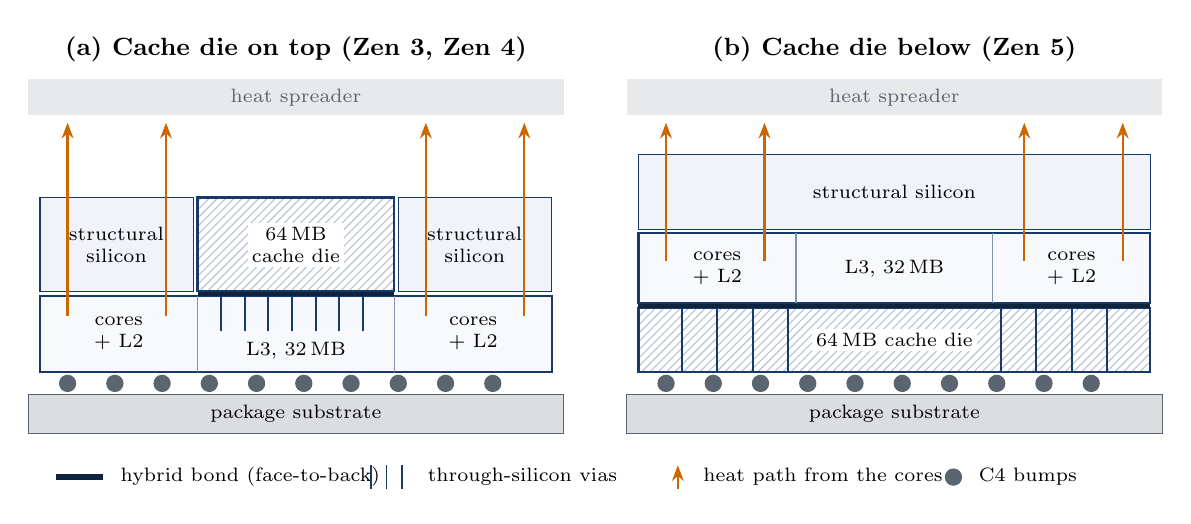
\begin{tikzpicture}[x=1cm,y=1cm,
  lay/.style={font=\scriptsize,align=center},
  hp/.style={-{Stealth[length=2mm]},orange!80!black,thick},
  ttl/.style={font=\small\bfseries,anchor=south}]
\newcommand{\base}[1]{%
  \filldraw[fill=draftgray!22,draw=draftgray] (#1-0.15,0) rectangle (#1+6.65,0.5);
  \node[lay] at (#1+3.25,0.25) {package substrate};
  \foreach \x in {0.35,0.95,...,6.2}{\fill[draftgray] (#1+\x,0.64) circle (0.11);}
  \fill[draftgray!14] (#1-0.15,4.05) rectangle (#1+6.65,4.5);
  \node[lay,text=draftgray] at (#1+3.25,4.27) {heat spreader};}
\begin{scope}
\base{0}
\filldraw[fill=draftlight!55,draw=draftblue,thick] (0,0.78) rectangle (6.5,1.75);
\draw[draftblue!55] (2.0,0.78) -- (2.0,1.75) (4.5,0.78) -- (4.5,1.75);
\node[lay] at (1.0,1.27) {cores\\+ L2};
\node[lay] at (5.5,1.27) {cores\\+ L2};
\node[lay] at (3.25,1.05) {L3, 32\,MB};
\foreach \x in {2.3,2.6,...,4.3}{\draw[draftblue,line width=0.7pt] (\x,1.3) -- (\x,1.75);}
\draw[draftblue!60!black,line width=2pt] (2.0,1.78) -- (4.5,1.78);
\filldraw[fill=draftlight,draw=draftblue] (0,1.81) rectangle (1.95,3.0);
\filldraw[fill=draftlight,draw=draftblue] (4.55,1.81) rectangle (6.5,3.0);
\fill[pattern=north east lines,pattern color=draftblue!30] (2.0,1.81) rectangle (4.5,3.0);
\draw[draftblue,thick] (2.0,1.81) rectangle (4.5,3.0);
\foreach \x in {0.35,1.6,4.9,6.15}{\draw[hp] (\x,1.5) -- (\x,3.95);}
\node[lay] at (0.97,2.4) {structural\\silicon};
\node[lay] at (5.52,2.4) {structural\\silicon};
\node[lay,fill=white,inner sep=1.5pt] at (3.25,2.4) {64\,MB\\cache die};
\node[ttl] at (3.25,4.6) {(a) Cache die on top (Zen~3, Zen~4)};
\end{scope}
\begin{scope}[xshift=7.6cm]
\base{0}
\fill[pattern=north east lines,pattern color=draftblue!30] (0,0.78) rectangle (6.5,1.6);
\draw[draftblue,thick] (0,0.78) rectangle (6.5,1.6);
\node[lay,fill=white,inner sep=1.5pt] at (3.25,1.19) {64\,MB cache die};
\foreach \x in {0.55,1.0,1.45,1.9,4.6,5.05,5.5,5.95}{\draw[draftblue,line width=0.7pt] (\x,0.78) -- (\x,1.6);}
\draw[draftblue!60!black,line width=2pt] (0,1.63) -- (6.5,1.63);
\filldraw[fill=draftlight!55,draw=draftblue,thick] (0,1.66) rectangle (6.5,2.55);
\draw[draftblue!55] (2.0,1.66) -- (2.0,2.55) (4.5,1.66) -- (4.5,2.55);
\node[lay] at (3.25,2.1) {L3, 32\,MB};
\filldraw[fill=draftlight,draw=draftblue] (0,2.6) rectangle (6.5,3.55);
\foreach \x in {0.35,1.6,4.9,6.15}{\draw[hp] (\x,2.2) -- (\x,3.95);}
\node[lay] at (3.25,3.07) {structural silicon};
\node[lay] at (1.0,2.1) {cores\\+ L2};
\node[lay] at (5.5,2.1) {cores\\+ L2};
\node[ttl] at (3.25,4.6) {(b) Cache die below (Zen~5)};
\end{scope}
\begin{scope}[yshift=-0.55cm]
\draw[draftblue!60!black,line width=2pt] (0.2,0) -- (0.8,0); \node[lay,anchor=west] at (0.9,0) {hybrid bond (face-to-back)};
\foreach \x in {4.2,4.4,4.6}{\draw[draftblue,line width=0.7pt] (\x,-0.15) -- (\x,0.15);} \node[lay,anchor=west] at (4.8,0) {through-silicon vias};
\draw[hp] (8.1,-0.15) -- (8.1,0.15); \node[lay,anchor=west] at (8.3,0) {heat path from the cores};
\fill[draftgray] (11.6,0) circle (0.11); \node[lay,anchor=west] at (11.8,0) {C4 bumps};
\end{scope}
\end{tikzpicture}
\caption[The two stack arrangements of 3D V-Cache]{The two stack arrangements of 3D V-Cache, drawn from AMD's comparison \cite[slide~7]{lambertHeterogenousIntegrationHigh2025} and descriptions \cite{wuu2022vcache,alam2ndGeneration3D2024,cozmaAMDs9800X3D2nd2024}. In (a) the cache die sits over the CCD's central L3 and the cores lie under structural silicon dies; in (b) the cache die, now the full width of the CCD, carries the through-silicon vias and the cores sit directly beneath a single structural layer. Schematic; not to scale.}
\label{fig:vcache-generations}
\end{figure}


\subsection{Manufacturing: thinning, assembly, yield and test}
\label{sec:manufacturing}
Stacking adds steps that a planar die does not need. The CCD is thinned, to about 20\,\textmu m in the cache-on-top parts \cite{cozmaAMDs9800X3D2nd2024}; a die that thin cannot support itself, which is one reason for the structural silicon \cite[slide~12]{wuu2022vcache}. Support silicon then restores the stack to the height of an ordinary CCD, so that server packages with and without V-Cache are the same \cite[slide~17]{wuu2022vcache}. Each of these steps costs money and adds a new way for a part to fail. \Cref{fig:stack-process} collects the extra steps described in this part.

\begin{figure}[htbp]
\centering
\begin{tikzpicture}[x=1cm,y=1cm,
  st/.style={draw=draftblue,thick,fill=draftlight,rounded corners=2pt,font=\scriptsize,align=center,text width=3.4cm,minimum height=0.95cm},
  alt/.style={draw=todored,fill=todored!8,rounded corners=2pt,font=\scriptsize,align=center,text width=3.3cm,minimum height=0.95cm},
  grp/.style={font=\scriptsize\bfseries,text=draftgray,anchor=east},
  arr/.style={-{Stealth[length=2mm]},draftblue,thick}]
\node[st] (t1) at (0,0) {Die-to-wafer flow: test CCD and cache dies; keep only known-good dies};
\node[alt,text width=3.4cm,draw=draftgray,fill=white] (t0) at (0,1.6) {Finished CCD and cache-die wafers};
\node[st] (t2) at (0,-1.7) {Form TSVs in the CCD and thin it (to about 20\,\textmu m in the cache-on-top parts)};
\node[st] (t3) at (0,-3.4) {Prepare bonding surfaces: oxide ending in Si--OH, copper pads slightly recessed};
\node[st] (b1) at (0,-5.4) {Place cache die on CCD at room temperature: oxide surfaces held by hydrogen bonds};
\node[st] (b2) at (0,-7.1) {Anneal: Si--O--Si bonds form, water released; copper diffuses and joins the pads};
\node[st] (f1) at (0,-9.1) {Add structural silicon: supports the thin CCD, conducts heat, restores standard height};
\node[st] (f2) at (0,-10.8) {Package as an ordinary CCD (same height with or without V-Cache)};
\foreach \a/\b in {t1/t2,t2/t3,t3/b1,b1/b2,b2/f1,f1/f2} \draw[arr] (\a) -- (\b);
\node[grp] at (-2.2,-1.7) {prepare};
\node[grp] at (-2.2,-6.25) {bond};
\node[grp] at (-2.2,-9.95) {finish};
\draw[draftgray,thin] (-2.05,0.5) -- (-2.05,-4.0) (-2.05,-4.8) -- (-2.05,-7.7) (-2.05,-8.5) -- (-2.05,-11.4);
\node[alt] (w2w) at (5.4,2.2) {Wafer-to-wafer: bond whole wafers untested; die yields multiply ($0.8542 \times 0.9223 = 78.8\%$ in \cref{tab:stack-yield})};
\node[st,text width=3.3cm] (d2w) at (5.4,-0.6) {Die-to-wafer: only tested good dies are bonded; dies may differ in size (V-Cache: 41 on 81\,mm$^2$)};
\draw[arr] (t0) -- (t1);
\draw[-{Stealth[length=2mm]},todored,thick,dashed] (t0.east) -- node[above,sloped,font=\scriptsize,text=todored]{no test} (w2w.west);
\draw[arr,dashed] (t1.east) -- (d2w.west);
\end{tikzpicture}
\caption[The steps that a V-Cache CCD needs and a planar one does not, grouped by purpose]{The steps that a V-Cache CCD needs and a planar one does not, grouped by purpose. The sources describe the steps but not their exact order in AMD's production flow, so the order shown is indicative. Sources: thinning \cite{cozmaAMDs9800X3D2nd2024}; bonding chemistry \cite[slide~9]{alam2ndGeneration3D2024}; structural silicon and package height \cite[slides~12, 17]{wuu2022vcache}; die-to-wafer against wafer-to-wafer \cite{dongSystemlevelCostAnalysis2009}, \cite[slide~10]{alam2ndGeneration3D2024}.}
\label{fig:stack-process}
\end{figure}


\textbf{Die-to-wafer or wafer-to-wafer?} Dies can be bonded one at a time onto a wafer of other dies (die-to-wafer, D2W), or two whole wafers can be bonded together (wafer-to-wafer, W2W). Dong and Xie summarise the trade-off: D2W can achieve a higher yield because each die can be tested first and only \emph{known-good dies} (KGD) stacked, whereas W2W needs no test before bonding and is easier to align, with higher throughput, at the cost of yield \cite[sec.~IV.C]{dongSystemlevelCostAnalysis2009}. AMD's 2024 comparison adds that in D2W the top and bottom dies need not be the same size and that D2W allows more heterogeneous integration, while W2W requires dies of the same or similar size \cite[slide~10]{alam2ndGeneration3D2024}. V-Cache stacks a 41\,mm$^2$ cache die on an 81\,mm$^2$ CCD, dies of different sizes from different wafers, so it falls on the D2W side of this comparison.

Dong and Xie's cost model shows why testing before bonding matters. For an $N$-layer stack bonded die-to-wafer, the cost of the bare stack is
\begin{equation}
  C_{\mathrm{D2W}} \;=\; \frac{\sum_{i=1}^{N} \left(C_{\mathrm{die},i} + C_{\mathrm{KGD\,test}}\right)/Y_{\mathrm{die},i} \;+\; (N-1)\,C_{\mathrm{bonding}}}{Y_{\mathrm{bonding}}^{\,N-1}},
  \label{eq:d2w-cost}
\end{equation}
while for wafer-to-wafer bonding the die yields multiply:
\begin{equation}
  C_{\mathrm{W2W}} \;=\; \frac{\sum_{i=1}^{N} C_{\mathrm{die},i} \;+\; (N-1)\,C_{\mathrm{bonding}}}{\prod_{i=1}^{N} Y_{\mathrm{die},i} \; Y_{\mathrm{bonding}}^{\,N-1}}
  \label{eq:w2w-cost}
\end{equation}
\cite[Eqs.~16--17]{dongSystemlevelCostAnalysis2009}. In W2W, a defect in either die scraps the whole stack, so the stack's yield is as low as that of a single large die; Dong and Xie find W2W stacking always more expensive than 2D in their study, and D2W cheaper than W2W from the yield perspective \cite[sec.~IV.C]{dongSystemlevelCostAnalysis2009}.

\textbf{Does stacking save silicon?} Compare a hypothetical planar CCD with all 96\,MB of L3 on one die against the actual two-die stack, using the yield model of \cref{eq:yield} with $D_0 = 0.2$\,cm$^{-2}$ and $Y_{\mathrm{wafer}} = 1$. The planar die is taken as the sum of the two real dies, $81 + 41 = 122$\,mm$^2$; this ignores the area of the TSVs and the possibility of a denser layout, so it is only an approximation. \Cref{tab:stack-yield} gives the result.

\begin{table}[htbp]
  \centering
  \caption[Silicon consumed per good part for a planar 96\,MB CCD and the stacked design]{Silicon consumed per good part for a planar 96\,MB CCD and the stacked design (Murphy model, $D_0 = 0.2$\,cm$^{-2}$; illustrative).}
  \label{tab:stack-yield}
  \small
  \begin{tabularx}{\textwidth}{@{}>{\raggedright\arraybackslash}X>{\raggedright\arraybackslash}p{2.2cm}>{\raggedright\arraybackslash}p{2.9cm}>{\raggedright\arraybackslash}p{4.0cm}@{}}
    \toprule
    \textbf{Design} & \textbf{Die area(s)} & \textbf{Modelled yield} & \textbf{Silicon per good part} \\
    \midrule
    Planar CCD with 96\,MB L3 & 122\,mm$^2$ & 79.1\% & 154\,mm$^2$ \\
    Stack, dies tested first (D2W) & 81 + 41\,mm$^2$ & 85.4\% and 92.2\% & $94.8 + 44.5 = 139$\,mm$^2$ $\div\,Y_{\mathrm{bonding}}$ \\
    Stack, untested (W2W) & 81 + 41\,mm$^2$ & $0.8542 \times 0.9223 = 78.8\%$ & $122/0.788 = 155$\,mm$^2$ $\div\,Y_{\mathrm{bonding}}$ \\
    \bottomrule
  \end{tabularx}
\end{table}

With known-good-die testing, the stack consumes about 10\% less silicon than the planar die, as long as bonding loses fewer than about 10\% of stacks ($139/154 \approx 0.90$). With $D_0 = 0.1$ the saving shrinks to about 5\%, and with $D_0 = 0.3$ it grows to about 14\%. Without testing, the stack has almost exactly the planar die's yield, as Dong and Xie's analysis predicts, and gains nothing. The silicon saving is modest; thinning, bonding and testing all cost extra, so on this measure alone stacking is not obviously cheaper. The stronger economic argument is the one AMD gives: \emph{product flexibility} \cite[slide~6]{wuu2022vcache}. The same 81\,mm$^2$ CCD is sold with or without a cache die, so only the products that need 96\,MB pay for it, while a planar 122\,mm$^2$ CCD would charge every product for the larger die.

\textbf{Silicon across a product line.} The flexibility argument can be put in the same units as \cref{tab:stack-yield}. \Cref{app:product-line} compares, in silicon per good part, three ways of building a product line in which some parts need 96\,MB of L3: one planar 96\,MB die for everything, two separate planar dies, and one CCD with an optional cache die. Against the single large die, stacking saves about a third of the silicon when few parts need the large cache, because the parts that do not need it no longer pay for it. Against two planar dies, the saving in silicon is only a few per cent, so stacking's real advantage there is outside the calculation: one CCD design instead of two, and a product mix decided at assembly rather than when wafers are started. This is how AMD describes its products: the Zen~3 V-Cache parts use a thinned version of the standard CCD and fit the same server package \cite[slide~17]{wuu2022vcache}, and in the fourth-generation EPYC processors the additional cache is stacked ``on top of each CPU die'' of the standard design \cite{advancedmicrodevicesinc.4thGenAMD2023}.

The node of the cache die adds a second, separate saving. In the Zen~4 generation the CCD moved to 5\,nm while the cache die stayed on 7\,nm \cite{alam2ndGeneration3D2024}. AMD's own chart of normalised cost per yielded mm$^2$ rises by roughly a third from 7\,nm to 5\,nm (read from the chart; approximate), while the same slide shows SRAM area scaling falling behind logic at those nodes \cite[slide~6]{wuu2022vcache}. A planar Zen~4 CCD with 96\,MB would have placed its extra 64\,MB of SRAM on the more expensive node, where it shrinks less than logic does. Stacking lets the SRAM stay on the older, cheaper node while the cores move on, the same reasoning that keeps the I/O die on an older node in the chiplet split (\cref{sec:yield-cost}).

\textbf{Reliability.} A bonded interface must survive years of heating and cooling. AMD reports that packaged Zen~4 V-Cache parts passed 96 hours of unbiased highly accelerated stress testing, 2500 temperature cycles and 1000 hours of high-temperature storage, with no apparent damage to the bond interface \cite[slide~14]{alam2ndGeneration3D2024}. These are AMD's qualification results, not independent tests.

\textbf{Co-design.} AMD's own summary of the project is that ``product definition and design [were] co-optimized up front with technology development'' \cite[slide~33]{wuu2022vcache}. The TSV columns, power channels and isolation circuits had to be in the CCD before the first V-Cache product existed, and the CCD's floorplan, with the L3 at the centre and the cores at the edges, made a cool, central place for the cache die. Stacked cache was therefore a design decision taken years before it shipped, not a packaging option added at the end.

\section{Workloads That Benefit From a Larger LLC}
\label{sec:vcache-workloads}

AMD's figures for V-Cache in games come from two different comparisons. Its Hot Chips~33 comparison of a 12-core 3D-chiplet prototype with the 12-core Ryzen~9 5900X, both fixed at 4.0\,GHz, reports gains from 1.04$\times$ to 1.25$\times$ across five games, 15\% on average \cite[slide~19]{swaminathanAdvancedPackagingEnabling2021}. Holding frequency fixed is valuable because it isolates the cache effect, but the result covers only the disclosed games and configuration and should not be generalised.

The ISSCC~2022 presentation adds product results, again from AMD's own testing \cite[slides~29, 31, 35]{wuu2022vcache}. The eight-core Ryzen~7 5800X3D is reported as about 15\% faster in games than the twelve-core Ryzen~9 5900X at 1080p with high settings, ranging from up to 1.36$\times$ in one title to a tie in another. On servers, a 16-core EPYC with V-Cache completed about 66\% more electronic-design jobs (register-transfer-level, or RTL, simulation of chip designs) per hour than a 16-core EPYC~73F3 without it. The spread from a tie to 1.36$\times$ already illustrates the workload dependence predicted in \cref{sec:miss-classes}; \cref{sec:confounds} discusses what else differs between the compared parts.

The miss classification of \cref{sec:miss-classes} predicts which workloads should benefit. A larger L3 removes capacity misses, so the gain depends on where a workload's working set lies relative to the 32\,MB and 96\,MB capacities:
\begin{itemize}
  \item \textbf{Working set already within 32\,MB.} Few capacity misses remain to remove, and every L3 hit pays the extra four cycles. Little or no gain, possibly a small loss.
  \item \textbf{Working set between 32\,MB and 96\,MB, with reuse.} Many accesses that went to memory now hit in the L3. This is where large gains are expected.
  \item \textbf{Working set far larger than 96\,MB, or streaming with little reuse.} The data still does not fit or is not reused, so the miss rate barely changes.
\end{itemize}
Mittal and Vetter note that modern scale-out workloads such as business analytics and web search can demand hundreds of megabytes of last-level cache \cite[sec.~1]{mittalSurveyTechniquesArchitecting2016}. AMD's gaming and RTL-simulation results above fit this picture, but they are vendor results and Part~\ref{part:case-study} examines them more critically.

Independent measurements support this classification. Lam measured each CCD of a Ryzen~9 7950X3D separately, with boost disabled and both CCDs held at 4.2\,GHz, and used performance counters to compare IPC and L3 hit rate \cite{lamAMDs7950X3DZen2023}. Because clock, core design, memory and software are identical, the differences isolate the cache. Workloads with many L3 misses gained most: IPC rose by over 19\% in \emph{Call of Duty: Black Ops Cold War}, whose hit rate rose by 47\%, and by 13\% in \emph{Cyberpunk 2077} (from 1.26 to 1.43). Workloads with few misses to remove gained little: libx264 video encoding, with 1.48 L3 misses per thousand instructions, gained 4.9\%, less than the plain CCD's 7\% clock advantage, and a flight simulator with only 0.35 misses per thousand instructions lost a little IPC, which Lam suggests is likely due to the added latency. These are the first two classes above, measured directly (\cref{fig:lam-ipc}); \cref{sec:tradeoff-example} works through the libx264 case with \cref{eq:vcache-tradeoff}.

\begin{figure}[htbp]
\centering
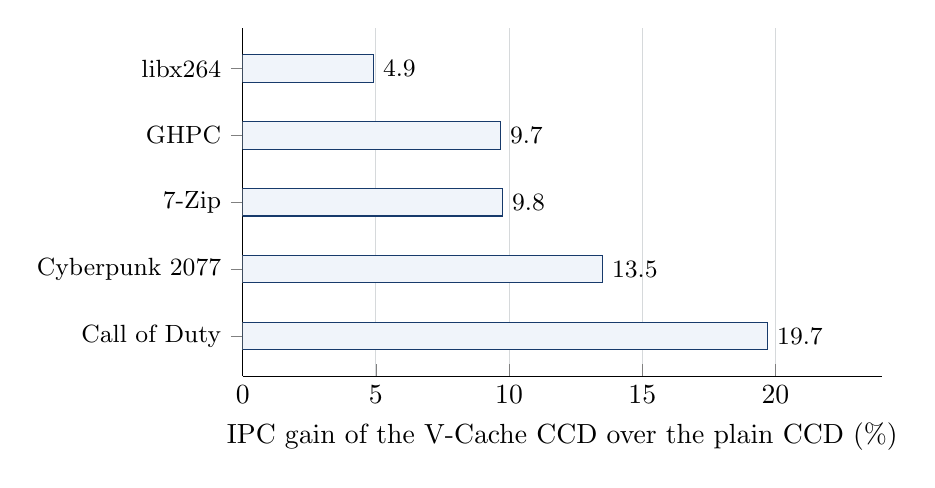
\begin{tikzpicture}
\begin{axis}[
  xbar, bar width=10pt, width=0.8\textwidth, height=6.0cm,
  xmin=0, xmax=24, xlabel={IPC gain of the V-Cache CCD over the plain CCD (\%)},
  symbolic y coords={libx264,GHPC,7-Zip,Cyberpunk 2077,Call of Duty},
  ytick=data, y dir=reverse, yticklabel style={font=\small},
  nodes near coords, nodes near coords style={font=\small,anchor=west},
  point meta=explicit symbolic,
  xmajorgrids, grid style={draftgray!25}, axis y line*=left, axis x line*=bottom,
  enlarge y limits=0.15]
\addplot[fill=draftlight,draw=draftblue] coordinates {
  (4.9,libx264)[4.9]
  (9.67,GHPC)[9.7]
  (9.75,7-Zip)[9.8]
  (13.5,Cyberpunk 2077)[13.5]
  (19.7,Call of Duty)[19.7]};
\end{axis}
\end{tikzpicture}
\caption[IPC gain from 3D V-Cache with clock, core design and memory held equal]{IPC gain from 3D V-Cache with clock, core design and memory held equal: the two CCDs of one Ryzen~9 7950X3D, both fixed at 4.2\,GHz, measured with performance counters by Lam \cite{lamAMDs7950X3DZen2023}. Cyberpunk~2077 is computed from the reported IPC of 1.26 and 1.43; the Call of Duty value is computed from the IPC of 0.71 and 0.85 read from Lam's chart (the text says ``over 19\%''). A sixth workload, a flight simulator with very few L3 misses, lost a small, unquantified amount of IPC and is not plotted.}
\label{fig:lam-ipc}
\end{figure}

HPC studies show the third class. On a memory-bound proxy application, Domke \emph{et al.} found that Milan-X was up to 3.4$\times$ faster than Milan, but only for a subset of problem sizes \cite{domkeLocusPerformanceQuantifying2023}. Lawenda \emph{et al.} found the same pattern in OpenFOAM: Milan-X was up to 1.54$\times$ faster than Milan for the mesh size that best fits its larger cache, the advantage fell to 1.24$\times$ for the largest mesh, and on some smaller meshes Milan-X was up to 19\% slower. The larger L3 cut the L3 miss rate by up to 30 percentage points \cite{lawendaEvaluatingImpactL32025}. On desktop software, Phoronix's 420-test comparison of the eight-core Ryzen~7 5800X3D with the eight-core 5800X found large V-Cache leads in a minority of tests, while the 5800X won, mostly by a couple of percent, where the cache could not be used and its slightly higher clocks paid off \cite{larabelAMDRyzen72022}.

\section{Summary of Part IV}
Applying the three-part test to 3D-stacked cache:
\begin{itemize}
  \item \textbf{Bottleneck addressed.} The area, yield, wire-length and power costs of growing an SRAM cache in the plane of the compute die, made worse by SRAM's slowing area scaling (\cref{sec:planar-limits}).
  \item \textbf{Benefit.} Three times the L3 per CCD (32 to 96\,MB) for four extra cycles of latency, with AMD's quoted peak of more than 2\,TB/s (not reproduced by independent CCD-wide tests, \cref{sec:vcache-access}) and no change to the package footprint or the cache hierarchy above the L3 \cite{wuu2022vcache,amd2022epyc7003}.
  \item \textbf{New trade-offs.} An altered heat path from the cores, power delivery through TSVs, die thinning, bonding and test complexity, a second die to pay for, and a benefit that depends strongly on the workload.
\end{itemize}

The calculations of this part make these points quantitative. The 9\,\textmu m bond pitch gives about sixteen times the connection density of micro-bumps (\cref{sec:density-example}), which allows a wide, parallel interface in little area and helps keep the latency cost to four cycles. Applied to Lam's libx264 measurements, the simple trade-off of \cref{eq:vcache-tradeoff} gives a range of 3--14\% that brackets the measured gain (\cref{sec:tradeoff-example}). The yield model suggests that stacking with tested dies saves only about a tenth of the silicon of an equivalent planar die (\cref{tab:stack-yield}). The economic case therefore rests mainly on product flexibility: one CCD with an optional cache die uses about as little silicon as two separate planar designs while needing only one design, and lets the SRAM stay on an older node (\cref{tab:product-line-silicon}). The heat path, which the cache-on-top parts managed with structural silicon, is the reason AMD gives for inverting the stack in Zen~5 (\cref{sec:thermal-evidence}); the lower clocks of those parts are attributed partly to the stacked cache's voltage tolerance as well. The inverted part still clocks about 5.5\% below its plain counterpart with an equal voltage limit, which suggests that factors besides the two named in the sources remain. Part~\ref{part:case-study} now turns from the mechanism to the evidence across products.
\clearpage
\part{AMD Case Study and Quantitative Analysis}
\label{part:case-study}
\Cref{fig:mindmap-case-study} maps the topics of this part.

\mapfigure{%
\node[mmroot] (r) {AMD case study};
\node[mmbox,mmlevel1,fill=mmCFE0F4] (b0) at (0.00,3.60) {Generations};
\draw[mmbig] (r) -- (b0);
\node[mmlevel2,mmbox,fill=mmF9D7AF] (b0c0) at (-3.05,5.35) {Zen~2: two L3s per CCD};
\draw[mmsmall] (b0.north) to[out=90,in=-90] (b0c0.south);
\node[mmlevel2,mmbox,fill=mmF9D7AF] (b0c1) at (0.00,5.35) {Zen~3: one 32\,MB L3};
\draw[mmsmall] (b0.north) to[out=90,in=-90] (b0c1.south);
\node[mmlevel2,mmbox,fill=mmF9D7AF] (b0c2) at (3.05,5.35) {X3D: Zen~3, 4, 5};
\draw[mmsmall] (b0.north) to[out=90,in=-90] (b0c2.south);
\node[mmbox,mmlevel1,fill=mmCFE7E1] (b1) at (4.07,2.20) {Comparison pairs};
\draw[mmbig] (r) -- (b1);
\node[mmlevel2,mmbox,fill=mmF9D7AF] (b1c0) at (7.67,3.65) {7763 / 7773X};
\draw[mmsmall] (b1.east) to[out=0,in=180] (b1c0.west);
\node[mmlevel2,mmbox,fill=mmF9D7AF] (b1c1) at (7.67,2.20) {5800X / 5800X3D};
\draw[mmsmall] (b1.east) to[out=0,in=180] (b1c1.west);
\node[mmlevel2,mmbox,fill=mmF9D7AF] (b1c2) at (7.67,0.75) {7950X3D: two CCDs};
\draw[mmsmall] (b1.east) to[out=0,in=180] (b1c2.west);
\node[mmbox,mmlevel1,fill=mmF4AAA2] (b2) at (4.07,-2.20) {Kinds of evidence};
\draw[mmbig] (r) -- (b2);
\node[mmlevel2,mmbox,fill=mmCFE7E1] (b2c0) at (7.67,-0.75) {AMD-reported};
\draw[mmsmall] (b2.east) to[out=0,in=180] (b2c0.west);
\node[mmlevel2,mmbox,fill=mmCFE7E1] (b2c1) at (7.67,-2.20) {Independent reviews};
\draw[mmsmall] (b2.east) to[out=0,in=180] (b2c1.west);
\node[mmlevel2,mmbox,fill=mmCFE7E1] (b2c2) at (7.67,-3.65) {HPC studies};
\draw[mmsmall] (b2.east) to[out=0,in=180] (b2c2.west);
\node[mmbox,mmlevel1,fill=mmF9D7AF] (b3) at (0.00,-3.60) {Latency};
\draw[mmbig] (r) -- (b3);
\node[mmlevel2,mmoval,fill=mmDCCFF6] (b3c0) at (-3.05,-5.35) {3--4 extra L3 cycles};
\draw[mmsmall] (b3.south) to[out=-90,in=90] (b3c0.north);
\node[mmlevel2,mmbox,fill=mmDCCFF6] (b3c1) at (0.00,-5.35) {Flat to beyond 64\,MB};
\draw[mmsmall] (b3.south) to[out=-90,in=90] (b3c1.north);
\node[mmlevel2,mmoval,fill=mmDCCFF6] (b3c2) at (3.05,-5.35) {TLB effects mixed in};
\draw[mmsmall] (b3.south) to[out=-90,in=90] (b3c2.north);
\node[mmoval,mmlevel1,fill=mmDCCFF6] (b4) at (-4.07,-2.20) {Workload results};
\draw[mmbig] (r) -- (b4);
\node[mmlevel2,mmbox,fill=mmF4C2BB] (b4c0) at (-7.67,-0.75) {MiniFE up to 3.4$\times$};
\draw[mmsmall] (b4.west) to[out=180,in=0] (b4c0.east);
\node[mmlevel2,mmbox,fill=mmF4C2BB] (b4c1) at (-7.67,-2.20) {OpenFOAM 0.81--1.54$\times$};
\draw[mmsmall] (b4.west) to[out=180,in=0] (b4c1.east);
\node[mmlevel2,mmbox,fill=mmF4C2BB] (b4c2) at (-7.67,-3.65) {350 desktop tests};
\draw[mmsmall] (b4.west) to[out=180,in=0] (b4c2.east);
\node[mmbox,mmlevel1,fill=mmD6EBC6] (b5) at (-4.07,2.20) {Isolating the cache};
\draw[mmbig] (r) -- (b5);
\node[mmlevel2,mmoval,fill=mmDCCFF6] (b5c0) at (-7.67,3.65) {Fixed clocks};
\draw[mmsmall] (b5.west) to[out=180,in=0] (b5c0.east);
\node[mmlevel2,mmbox,fill=mmDCCFF6] (b5c1) at (-7.67,2.20) {Counters, clock correction};
\draw[mmsmall] (b5.west) to[out=180,in=0] (b5c1.east);
\node[mmlevel2,mmoval,fill=mmDCCFF6] (b5c2) at (-7.67,0.75) {Simulation (S0--S6)};
\draw[mmsmall] (b5.west) to[out=180,in=0] (b5c2.east);
}{[Overview of Part~\ref{part:case-study}]{Overview of Part~\ref{part:case-study}: the products, the comparisons, the kinds of evidence and the main results, with values as reported in \cref{sec:benchmarks,sec:confounds}; the simulation is \cref{sec:sim-study}.}}{fig:mindmap-case-study}

\section{Method for Analysing Published Evidence}
\label{sec:evidence-method}

The quantitative analysis uses published research and benchmarks (\cref{fig:evidence-method}), complemented by a simulation that changes one factor at a time (\cref{sec:sim-study}), which the group compared with its own Ryzen~5 5600X (\cref{app:5600x}). Published evidence is the most manageable option given that the group has no processor with stacked cache. Its limitation is dependence on the experimental conditions and measurements that others chose to publish; the analysis can only be as controlled as its sources.

\begin{figure}[htbp]
\centering
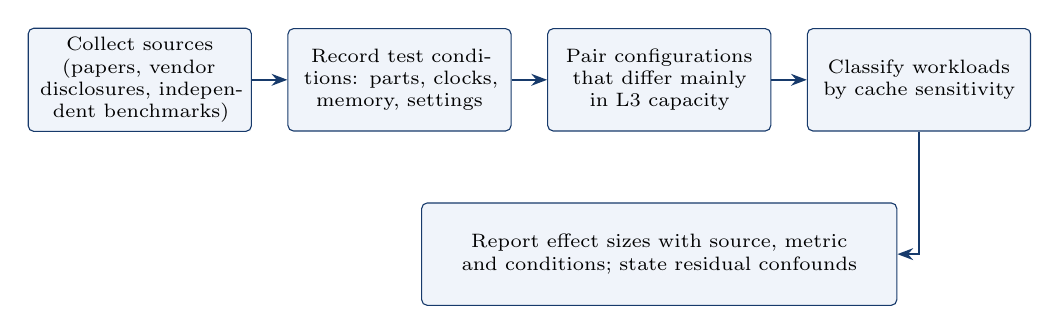
\begin{tikzpicture}[
  st/.style={draw=draftblue,fill=draftlight,rounded corners=2pt,align=center,text width=2.6cm,minimum height=1.3cm,font=\scriptsize},
  arr/.style={-{Stealth[length=2mm]},draftblue,thick}, node distance=0.45cm]
\node[st] (a) {Collect sources\\(papers, vendor disclosures, independent benchmarks)};
\node[st,right=of a] (b) {Record test conditions: parts, clocks, memory, settings};
\node[st,right=of b] (c) {Pair configurations that differ mainly in L3 capacity};
\node[st,right=of c] (d) {Classify workloads by cache sensitivity};
\node[st,below=0.9cm of c,text width=5.8cm] (e) {Report effect sizes with source, metric and conditions; state residual confounds};
\draw[arr] (a)--(b); \draw[arr] (b)--(c); \draw[arr] (c)--(d); \draw[arr] (d) |- (e);
\end{tikzpicture}
\caption[Evidence-analysis procedure for Part~V]{Evidence-analysis procedure for Part~V (published research and benchmarks; the group's own measurements on a Ryzen~5 5600X are in \cref{app:5600x}).}
\label{fig:evidence-method}
\end{figure}

Each source is recorded with: the processors compared; clock frequencies (fixed or boost); memory type, speed and timings; power limits; software and settings; the metric (for example, frames per second, IPC, runtime or throughput); and whether the source is the vendor or an independent party. Results are reported as relative changes with the source, metric and conditions stated, never as a single headline number.

\textbf{Source selection.} Sources are admitted in three tiers: peer-reviewed papers; independent benchmark publications that state their hardware, settings and method; and vendor material, which is used only when labelled as such. Every source used must have its PDF in the project's source folder. Where sources conflict, the one with the better-controlled comparison (\cref{sec:confounds}) is preferred and the disagreement is reported. Results across workloads are reported as ranges, and where a source gives them, as medians, rather than as averages that would hide their spread. Where this paper computes a summary itself, such as the geometric mean of \cref{sec:lam-detail}, it says so and gives the range beside it.

\section{From Zen 2 Chiplets to Zen 3 and 3D V-Cache}
\label{sec:zen-progression}

\begin{figure}[htbp]
\centering
\resizebox{\textwidth}{!}{%
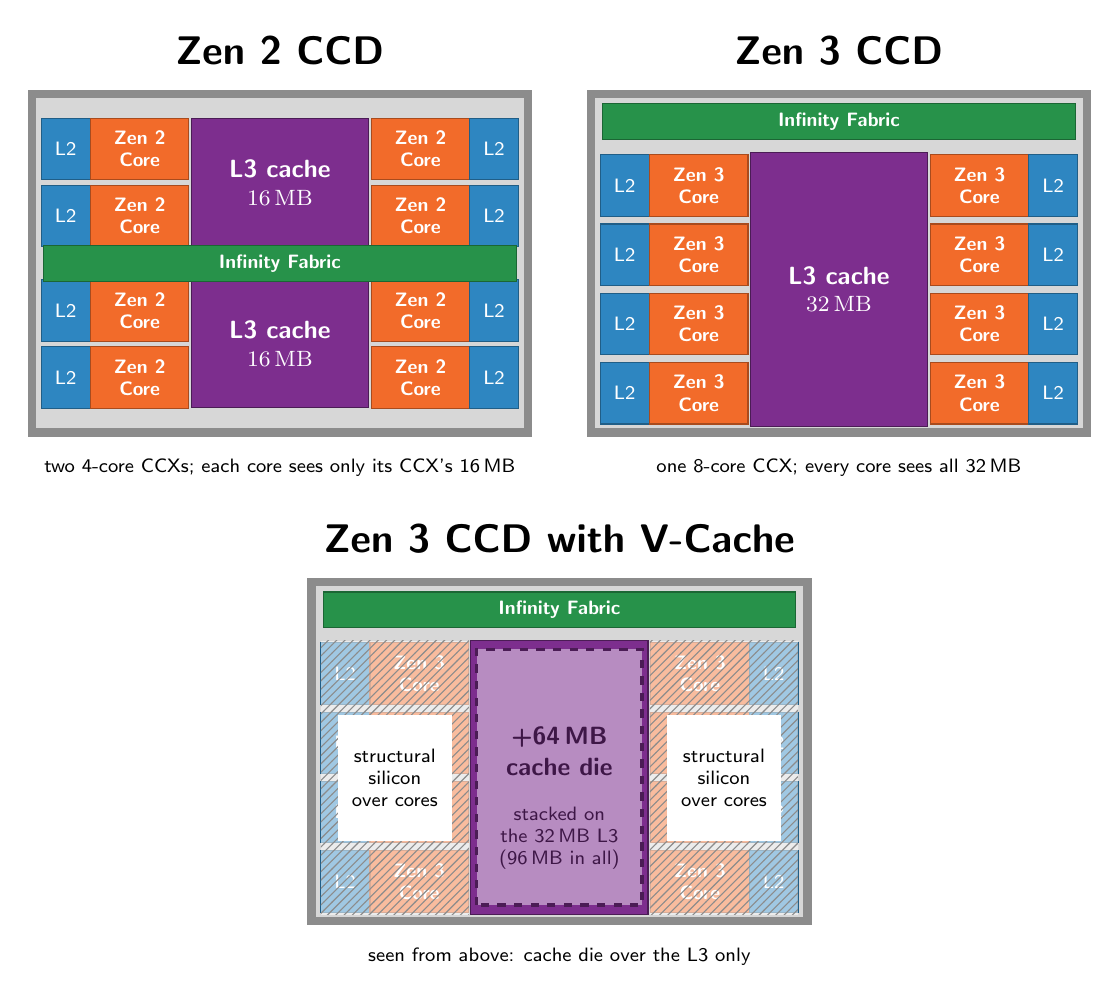
\begin{tikzpicture}[x=1cm,y=1cm,
  frame/.style={draw=ccdframe,line width=3pt,fill=ccdframe!35},
  core/.style={draw=ccdcore!70!black,fill=ccdcore,text=white,font=\sffamily\scriptsize\bfseries,align=center,minimum width=1.25cm,minimum height=0.78cm,inner sep=1pt},
  l2/.style={draw=ccdl2!70!black,fill=ccdl2,text=white,font=\sffamily\scriptsize,align=center,minimum width=0.62cm,minimum height=0.78cm,inner sep=0.5pt},
  l3/.style={draw=ccdl3!60!black,fill=ccdl3,text=white,font=\sffamily\small\bfseries,align=center},
  fab/.style={draw=ccdif!70!black,fill=ccdif,text=white,font=\sffamily\scriptsize\bfseries,minimum height=0.36cm},
  ttl/.style={font=\sffamily\Large\bfseries}]
\providecommand{\corepair}[4]{%
  \ifnum#4=1
    \node[l2] at (#1+0.31,#2) {L2}; \node[core] at (#1+1.25,#2) {#3\\Core};
  \else
    \node[core] at (#1+0.625,#2) {#3\\Core}; \node[l2] at (#1+1.56,#2) {L2};
  \fi}
\begin{scope}
\node[ttl] at (3.15,4.85) {Zen~2 CCD};
\draw[frame] (0,0) rectangle (6.3,4.3);
\foreach \y in {2.75,3.6}{\corepair{0.12}{\y}{Zen~2}{1}\corepair{4.31}{\y}{Zen~2}{0}}
\foreach \y in {0.7,1.55}{\corepair{0.12}{\y}{Zen~2}{1}\corepair{4.31}{\y}{Zen~2}{0}}
\node[l3,minimum width=2.25cm,minimum height=1.62cm] at (3.15,3.175) {L3 cache\\[-1pt]{\normalfont\footnotesize 16\,MB}};
\node[l3,minimum width=2.25cm,minimum height=1.62cm] at (3.15,1.125) {L3 cache\\[-1pt]{\normalfont\footnotesize 16\,MB}};
\node[fab,minimum width=6.0cm] at (3.15,2.15) {Infinity Fabric};
\node[font=\sffamily\scriptsize,align=center] at (3.15,-0.45) {two 4-core CCXs; each core sees only its CCX's 16\,MB};
\end{scope}
\begin{scope}[xshift=7.1cm]
\node[ttl] at (3.15,4.85) {Zen~3 CCD};
\draw[frame] (0,0) rectangle (6.3,4.3);
\node[fab,minimum width=6.0cm] at (3.15,3.95) {Infinity Fabric};
\foreach \y in {0.5,1.38,2.26,3.14}{\corepair{0.12}{\y}{Zen~3}{1}\corepair{4.31}{\y}{Zen~3}{0}}
\node[l3,minimum width=2.25cm,minimum height=3.48cm] at (3.15,1.82) {L3 cache\\[-1pt]{\normalfont\footnotesize 32\,MB}};
\node[font=\sffamily\scriptsize,align=center] at (3.15,-0.45) {one 8-core CCX; every core sees all 32\,MB};
\end{scope}
\begin{scope}[xshift=3.55cm,yshift=-6.2cm]
\node[ttl] at (3.15,4.85) {Zen~3 CCD with V-Cache};
\draw[frame] (0,0) rectangle (6.3,4.3);
\node[fab,minimum width=6.0cm] at (3.15,3.95) {Infinity Fabric};
\foreach \y in {0.5,1.38,2.26,3.14}{\corepair{0.12}{\y}{Zen~3}{1}\corepair{4.31}{\y}{Zen~3}{0}}
\node[l3,minimum width=2.25cm,minimum height=3.48cm] at (3.15,1.82) {};
\fill[white,opacity=0.55] (0.12,0.08) rectangle (2.0,3.56);
\fill[white,opacity=0.55] (4.3,0.08) rectangle (6.18,3.56);
\fill[pattern=north east lines,pattern color=ccdframe] (0.12,0.08) rectangle (2.0,3.56);
\fill[pattern=north east lines,pattern color=ccdframe] (4.3,0.08) rectangle (6.18,3.56);
\draw[fill=ccdl3!55!white,draw=ccdl3!60!black,line width=1.2pt,dashed] (2.1,0.2) rectangle (4.2,3.45);
\node[font=\sffamily\small\bfseries,text=ccdl3!50!black,align=center] at (3.15,2.15) {+64\,MB\\cache die};
\node[font=\sffamily\scriptsize,text=ccdl3!50!black,align=center] at (3.15,1.05) {stacked on\\the 32\,MB L3\\(96\,MB in all)};
\node[font=\sffamily\scriptsize,align=center,fill=white,inner sep=2pt,minimum width=1.45cm,minimum height=1.6cm] at (1.06,1.82) {structural\\silicon\\over cores};
\node[font=\sffamily\scriptsize,align=center,fill=white,inner sep=2pt,minimum width=1.45cm,minimum height=1.6cm] at (5.24,1.82) {structural\\silicon\\over cores};
\node[font=\sffamily\scriptsize,align=center] at (3.15,-0.45) {seen from above: cache die over the L3 only};
\end{scope}
\end{tikzpicture}}
\caption[Compute die organisation from Zen~2 to Zen~3 and Zen~3 with 3D V-Cache]{Compute die (CCD) organisation from Zen~2 to Zen~3 and Zen~3 with 3D V-Cache: cores (orange), private 512\,KB L2 caches (blue), L3 (purple) and the Infinity Fabric interface (green). Zen~2 splits the CCD into two four-core complexes with 16\,MB of L3 each; Zen~3 gives all eight cores one 32\,MB L3; V-Cache stacks a 64\,MB cache die over the central L3 and covers the cores only with structural silicon. Drawn from AMD's descriptions \cite{suggs2019zen2,amd2022epyc7003,wuu2022vcache}; a schematic, not a floorplan, and not to scale.}
\label{fig:zen-ccd-evolution}
\end{figure}

\Cref{tab:zen-progression} and \cref{fig:zen-ccd-evolution} summarise the changes in cache organisation that matter for this paper, using only AMD's published descriptions.

\begin{table}[htbp]
  \centering
  \caption[L3 organisation per compute die across the generations studied]{L3 organisation per compute die across the generations studied (AMD-published figures).}
  \label{tab:zen-progression}
  \small
  \begin{tabularx}{\textwidth}{@{}>{\raggedright\arraybackslash}p{3.3cm}>{\raggedright\arraybackslash}X>{\raggedright\arraybackslash}X>{\raggedright\arraybackslash}X@{}}
    \toprule
    & \textbf{Zen 2 CCD} & \textbf{Zen 3 CCD} & \textbf{Zen 3 CCD with 3D V-Cache} \\
    \midrule
    Cores per CCD & 8 & 8 & 8 \\
    CCX organisation & Two 4-core CCXs & One 8-core CCX & One 8-core CCX \\
    L3 shared by one core & Up to 16 MB (its CCX) & 32 MB & 96 MB \\
    L3 per CCD & 2 $\times$ 16 MB & 32 MB & 32 MB base + 64 MB stacked \\
    Private L2 per core & 512 KB & 512 KB & 512 KB \\
    CCD area & 74 mm$^2$ & 81 mm$^2$ & 81 mm$^2$ + 41 mm$^2$ cache die \\
    Added L3 latency & --- & --- & +4 cycles \\
    Sources & \cite{suggs2019zen2,naffziger2020chiplet} & \cite{amd2022epyc7003,wuu2022vcache} & \cite{amd2022epyc7003,wuu2022vcache} \\
    \bottomrule
  \end{tabularx}
\end{table}

Zen~3 kept the L3 capacity per CCD and changed its \emph{sharing}: each core can now use the whole 32\,MB rather than only its own CCX's 16\,MB \cite{amd2022epyc7003,suggs2019zen2}. 3D V-Cache then tripled the capacity seen by each core without changing the CCD's footprint or the sharing structure \cite{amd2022epyc7003,wuu2022vcache}. These two steps give a natural experiment for the effect of L3 capacity, as long as other differences are controlled (\cref{sec:confounds}).

\subsection{Zen~2 to Zen~3: a same-core-count comparison}
\label{sec:zen2-zen3}
The Zen~2 to Zen~3 step can be examined with two eight-core, single-CCD desktop parts. The Ryzen~7 3700X (Zen~2) and Ryzen~7 5800X (Zen~3) both have eight cores, sixteen threads and 32\,MB of L3, but the 3700X splits its L3 into two 16\,MB halves, one per four-core CCX, while the 5800X shares all 32\,MB among its eight cores \cite{suggs2019zen2,amd2022epyc7003}. They differ in other ways too: base and maximum boost clocks of 3.6 and 4.4\,GHz against 3.8 and 4.7\,GHz, and a TDP of 65\,W against 105\,W \cite{advancedmicrodevicesinc.AMDRyzen30002022}.

AMD attributes a 19\% IPC increase to Zen~3, citing the unified eight-core complex with direct access to 32\,MB of L3 among the core improvements. The figure comes from 25 workloads run at a locked 4\,GHz on the eight-core Ryzen~7 3800XT and 5800X, both with DDR4-3600 memory \cite[note~4]{advancedmicrodevicesinc.AMDLaunchesAMD2020}. Because clock, core count and memory are held equal, this is a cleaner comparison than most vendor figures. It still cannot separate the shared L3 from the many other changes to the Zen~3 core.

Independent testing of the two retail parts shows the combined effect. With the same DDR4-3200 CL14 memory, TechSpot measured the 5800X ahead of the 3700X by 22\% in Cinebench R20 multi-core and by 24\% and 19\% in 7-Zip compression and decompression. In rendering it led by 16\% in Blender, 30\% in V-Ray and 26\% in Corona, and elsewhere by 12\% in code compilation, 6\% in DaVinci Resolve, 14\% in Premiere Pro, 27\% in Photoshop and 23\% in After Effects \cite{waltonAMDRyzen72020}. During the multi-core Cinebench run the 5800X held about 4.55\,GHz, and it drew about 20\,W more than the 3700X \cite{waltonAMDRyzen72020}. These are whole-processor differences. The 5800X runs at higher clocks under a higher power limit and has a redesigned core, so the gains cannot be credited to the unified L3 alone. The gains are broad rather than concentrated in cache-sensitive work: the largest is in V-Ray, a multi-threaded renderer (30\%), and large gains also appear in Photoshop (27\%), which the reviewer describes as relying heavily on single-core performance \cite{waltonAMDRyzen72020}. In our reading, this points to the core and clock as much as to the cache.

Cache measurements give a more direct view. The FPS Review ran AIDA64's cache and memory benchmark on both processors with identical DDR4-3600 CL16 memory and the same fabric clock (1800\,MHz) \cite{justiceAMDRyzen72021}. Memory read bandwidth was the same, about 50.7\,GB/s on both, and memory latency fell from 68.8\,ns on the 3700X to 61.8\,ns on the 5800X. L3 read bandwidth was also nearly identical (633 against 631\,GB/s). L3 latency, however, \emph{rose} from 9.9\,ns to 10.9\,ns \cite{justiceAMDRyzen72021}. At the core clocks the tool reported during the runs (4.40 and 4.85\,GHz), this is roughly 44 cycles against 53 cycles. The figures come from screenshots of a single run on each processor, so the cycle counts are only approximate.

Chips and Cheese's latency measurements across Zen generations agree: unifying the two 16\,MB caches of a Zen~2 CCD into one 32\,MB cache added 7 to 8 cycles of L3 latency. By contrast, doubling the size of each L3 slice from Zen to Zen~2 added about 5 cycles and tripling it with V-Cache only 3 to 4, which suggests that enlarging slices is cheaper in latency than merging separate caches into one \cite{cozmaDeepDivingZen2022}. Chips and Cheese adds that how much of the 7 to 8 cycles came from AMD preparing the design for V-Cache cannot be known \cite{cozmaDeepDivingZen2022}. \Cref{fig:zen2-zen3-latency} plots the AIDA64 latencies.

\begin{figure}[htbp]
\centering
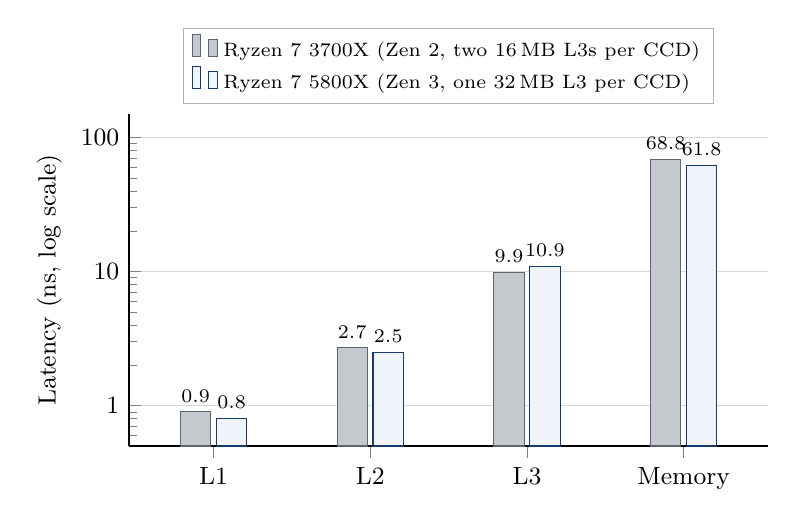
\begin{tikzpicture}
\begin{axis}[
  ybar, bar width=11pt, width=0.8\textwidth, height=5.8cm,
  ymode=log, ymin=0.5, ymax=150, log ticks with fixed point, log origin=infty,
  ylabel={Latency (ns, log scale)},
  symbolic x coords={L1,L2,L3,Memory}, xtick=data,
  nodes near coords, nodes near coords style={font=\scriptsize},
  point meta=rawy,
  ymajorgrids, grid style={draftgray!25}, axis x line*=bottom, axis y line*=left,
  legend style={at={(0.5,1.03)},anchor=south}, legend cell align=left, legend style={font=\scriptsize,draw=draftgray!50},
  enlarge x limits=0.18, label style={font=\small}, tick label style={font=\small}]
\addplot[fill=draftgray!35,draw=draftgray] coordinates {(L1,0.9) (L2,2.7) (L3,9.9) (Memory,68.8)};
\addlegendentry{Ryzen~7 3700X (Zen~2, two 16\,MB L3s per CCD)}
\addplot[fill=draftlight,draw=draftblue] coordinates {(L1,0.8) (L2,2.5) (L3,10.9) (Memory,61.8)};
\addlegendentry{Ryzen~7 5800X (Zen~3, one 32\,MB L3 per CCD)}
\end{axis}
\end{tikzpicture}
\caption[AIDA64 latency of a Zen~2 and a Zen~3 eight-core processor]{AIDA64 cache and memory latency of a Zen~2 and a Zen~3 eight-core processor with identical DDR4-3600 CL16 memory and the same 1800\,MHz fabric clock, from The FPS Review \cite{justiceAMDRyzen72021}. Unifying the L3 made it slower by about a nanosecond, while memory latency fell by 7\,ns; the 5800X also runs at a higher clock, so the nanosecond values mix the cache change with the clock change.}
\label{fig:zen2-zen3-latency}
\end{figure}


This result fits the trade-off described in \cref{sec:planar-limits}. Doubling the cache a core can reach, from 16 to 32\,MB, removes misses for working sets between the two sizes and the traffic between CCXs, but a larger shared array serving more cores takes longer to reach. The 5800X's faster single-threaded applications, in which the 32\,MB working-set limit rarely matters, therefore most likely owe their gains to the core and clock, not to faster cache access. Isolating the benefit of the unified L3 itself would require fixed-clock measurements of workloads with working sets between 16 and 32\,MB, or of communication between cores in different CCXs, which none of the sources in hand provides.

Two later generations extend the same pattern (\cref{tab:later-x3d}). With Zen~4, AMD kept the stack unchanged in principle but moved the CCD to 5\,nm while the cache die stayed at 7\,nm \cite{alam2ndGeneration3D2024}; on servers, up to twelve CCDs per package each reach 96\,MB of L3 with V-Cache, for up to 1152\,MB per socket \cite{advancedmicrodevicesinc.4thGenAMD2023}. With Zen~5, AMD inverted the stack so that the cache die sits below the CCD (\cref{sec:thermal-evidence}).

\begin{table}[htbp]
  \centering
  \caption[3D V-Cache across Zen generations]{3D V-Cache across Zen generations (AMD-published figures unless noted).}
  \label{tab:later-x3d}
  \small
  \begin{tabularx}{\textwidth}{@{}>{\raggedright\arraybackslash}p{2.0cm}>{\raggedright\arraybackslash}X>{\raggedright\arraybackslash}X>{\raggedright\arraybackslash}X@{}}
    \toprule
    & \textbf{Zen 3} & \textbf{Zen 4} & \textbf{Zen 5} \\
    \midrule
    Example parts & Ryzen~7 5800X3D; EPYC 7773X & Ryzen~7 7800X3D; EPYC 9684X & Ryzen~7 9800X3D \\
    CCD / cache die & 7\,nm / 7\,nm & 5\,nm / 7\,nm & 4\,nm (TSMC) / not stated \\
    Stack order & cache die on top of CCD & cache die on top of CCD & CCD on top of cache die \\
    L3 per V-Cache CCD & 96\,MB & 96\,MB & 96\,MB (32 + 64) \\
    Largest socket L3 & 768\,MB & 1152\,MB & --- \\
    Added L3 latency & 3--4 cycles (measured) & about 4 cycles (measured) & 4 cycles (measured) \\
    Sources & \cite{wuu2022vcache,amd2022epyc7003,cozmaDeepDivingZen2022} & \cite{alam2ndGeneration3D2024,advancedmicrodevicesinc.4thGenAMD2023,lamAMDs7950X3DZen2023} & \cite{advancedmicrodevicesinc.GamingLegendContinues2024,advancedmicrodevicesinc.AMDRyzen72024,lambertHeterogenousIntegrationHigh2025,cozmaAMDs9800X3D2nd2024} \\
    \bottomrule
  \end{tabularx}
\end{table}
AMD lists the Ryzen~7 9800X3D with 96\,MB of L3, cores made in TSMC's 4\,nm process and an I/O die in 6\,nm \cite{advancedmicrodevicesinc.AMDRyzen72024}; it does not state the process used for the cache die.

\section{Comparing Architectural Configurations}
\label{sec:config-compare}
The comparisons in this part rely on pairs of processors that differ mainly in L3 capacity. \Cref{tab:config-pairs} lists the pairs used and what else differs between them.

\begin{table}[htbp]
  \centering
  \caption[Processor pairs that differ mainly in L3 capacity]{Processor pairs that differ mainly in L3 capacity.}
  \label{tab:config-pairs}
  \small
  \begin{tabularx}{\textwidth}{@{}>{\raggedright\arraybackslash}p{3.3cm}>{\raggedright\arraybackslash}p{1.1cm}>{\raggedright\arraybackslash}p{2.2cm}>{\raggedright\arraybackslash}X>{\raggedright\arraybackslash}p{1.6cm}@{}}
    \toprule
    \textbf{Pair} & \textbf{Cores} & \textbf{L3} & \textbf{Other differences} & \textbf{Source} \\
    \midrule
    EPYC 7763 vs 7773X (Zen~3) & 64 & 256 vs 768\,MB & base clock 2.45 vs 2.20\,GHz; same 3.5\,GHz boost & \cite{larabelAMDEPYC7773X2022} \\
    Ryzen~7 5800X vs 5800X3D (Zen~3) & 8 & 32 vs 96\,MB & 5800X clocks slightly higher & \cite{larabelAMDRyzen72022} \\
    7950X3D: plain CCD vs V-Cache CCD (Zen~4) & 8 per CCD & 32 vs 96\,MB & plain CCD about 7\% faster at stock; identical when both are fixed at 4.2\,GHz & \cite{lamAMDs7950X3DZen2023} \\
    EPYC 9654 vs 9684X (Zen~4) & 96 & 384 vs 1152\,MB & all-core boost 3.55 vs 3.42\,GHz; base 2.40 vs 2.55\,GHz; same 3.70\,GHz maximum; default power 360 vs 400\,W & \cite{advancedmicrodevicesinc.AMDEPYC90042023} \\
    \bottomrule
  \end{tabularx}
\end{table}

\section{Published Benchmarks and Performance Measurements}
\label{sec:benchmarks}

The evidence falls into two groups: AMD-reported results (\cref{tab:amd-reported}) and independent measurements (\cref{tab:independent}).

\begin{table}[htbp]
  \centering
  \caption[AMD-reported performance figures relevant to this study]{AMD-reported performance figures relevant to this study (vendor claims, not independent measurements).}
  \label{tab:amd-reported}
  \small
  \begin{tabularx}{\textwidth}{@{}>{\raggedright\arraybackslash}X>{\raggedright\arraybackslash}p{4.4cm}>{\raggedright\arraybackslash}p{2.0cm}@{}}
    \toprule
    \textbf{Claim} & \textbf{Conditions stated} & \textbf{Source} \\
    \midrule
    About 15\% faster gaming, 8-core Ryzen~7 5800X3D vs 12-core Ryzen~9 5900X; per-title results from a tie to 1.36$\times$ & Six games at 1080p, high preset; both with DDR4-3600 and RTX~3080; AMD testing, Dec.\ 2021 & \cite[slides~29, 35]{wuu2022vcache} \\
    About 66\% more RTL-simulation jobs per hour (24.4 to 40.6), 16-core EPYC with V-Cache vs 16-core EPYC~73F3 & Synopsys VCS; same reference platform; AMD testing, Sept.\ 2021 & \cite[slides~31, 35]{wuu2022vcache} \\
    15\% average gaming uplift, 12-core 3D-chiplet prototype vs Ryzen~9 5900X & Both at the same fixed frequency; disclosed games only & \cite{swaminathanAdvancedPackagingEnabling2021} \\
    15\% IPC improvement from Zen to Zen~2 & Many simultaneous changes, including doubled L3 & \cite{suggs2019zen2} \\
    19\% IPC improvement from Zen~2 to Zen~3 (one AMD test, reported in both sources) & 25 workloads at a fixed 4\,GHz, 3800XT vs 5800X, equal memory; but a redesigned core as well as the unified L3 & \cite{advancedmicrodevicesinc.AMDLaunchesAMD2020}, \cite[slides~10, 35]{wuu2022vcache} \\
    19\% average memory-latency reduction, Rome vs Naples & Central IOD, decoupled clocks, optimised IFOP & \cite{naffziger2020chiplet} \\
    \bottomrule
  \end{tabularx}
\end{table}

\begin{table}[htbp]
  \centering
  \caption[Independent measurements of the effect of 3D V-Cache]{Independent measurements of the effect of 3D V-Cache.}
  \label{tab:independent}
  \small
  \begin{tabularx}{\textwidth}{@{}>{\raggedright\arraybackslash}X>{\raggedright\arraybackslash}p{4.6cm}>{\raggedright\arraybackslash}p{1.5cm}@{}}
    \toprule
    \textbf{Result} & \textbf{Conditions} & \textbf{Source} \\
    \midrule
    IPC $+4.9\%$ to $+19.7\%$ across five workloads (geometric mean $+11.4\%$ by the authors' calculation, \cref{sec:lam-detail}); one workload slightly negative & 7950X3D, each CCD at a fixed 4.2\,GHz; performance counters & \cite{lamAMDs7950X3DZen2023} \\
    Up to 3.4$\times$ on MiniFE for a subset of problem sizes & EPYC 7773X vs 7763, 64 cores each & \cite{domkeLocusPerformanceQuantifying2023} \\
    OpenFOAM from 0.81$\times$ to 1.54$\times$ (motorBike) and up to 1.47$\times$ (urban air pollution); L3 miss rate down by up to 30 points & EPYC 7773X vs 7763, dual socket, clocks not fixed & \cite{lawendaEvaluatingImpactL32025} \\
    gem5 $+7.6\%$, libx264 and 7-Zip about $+5\%$ on one CCD; Milan-X clocked about 5\% lower & Milan-X vs Milan cloud instances, clocks estimated & \cite{cozmaDeepDivingZen2022} \\
    Of 350 significant differences among 420 tests, 106 favour the 5800X3D (12 by 50\% or more) and 244 the 5800X (all but 3 by under 10\%) & Ryzen~7 5800X3D vs 5800X, Linux & \cite{larabelAMDRyzen72022} \\
    L3 latency $+3$ to $+4$ cycles & Milan-X, 7950X3D, 9800X3D & \cite{cozmaDeepDivingZen2022,lamAMDs7950X3DZen2023,cozmaAMDs9800X3D2nd2024} \\
    \bottomrule
  \end{tabularx}
\end{table}

The independent results agree with AMD's on direction but not on size: they show a wider spread, including small losses, and the best-controlled of them, Lam's fixed-frequency per-CCD measurements, shows single-digit to high-teen IPC gains rather than uniform double-digit speedups. \Cref{fig:vendor-vs-independent} shows the difference in spread.

\begin{figure}[htbp]
\centering
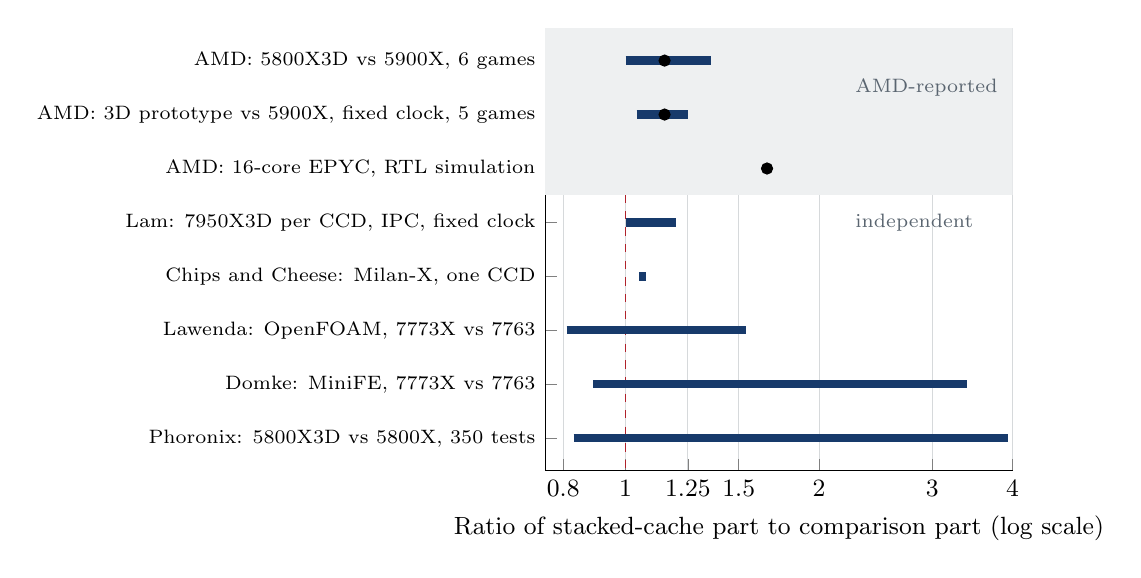
\begin{tikzpicture}
\begin{axis}[
  width=0.62\textwidth, height=7.2cm,
  xmode=log, xmin=0.75, xmax=4, ymin=0.4, ymax=8.6,
  xtick={0.8,1,1.25,1.5,2,3,4}, xticklabels={0.8,1,1.25,1.5,2,3,4},
  ytick={1,...,8}, y dir=reverse,
  yticklabels={{AMD: 5800X3D vs 5900X, 6 games},{AMD: 3D prototype vs 5900X, fixed clock, 5 games},{AMD: 16-core EPYC, RTL simulation},
    {Lam: 7950X3D per CCD, IPC, fixed clock},{Chips and Cheese: Milan-X, one CCD},{Lawenda: OpenFOAM, 7773X vs 7763},
    {Domke: MiniFE, 7773X vs 7763},{Phoronix: 5800X3D vs 5800X, 350 tests}},
  yticklabel style={font=\scriptsize},
  xlabel={Ratio of stacked-cache part to comparison part (log scale)},
  xmajorgrids, grid style={draftgray!25}, axis x line*=bottom, axis y line*=left,
  label style={font=\small}, tick label style={font=\small}]
\draw[todored,dashed] (axis cs:1,0.4) -- (axis cs:1,8.6);
\fill[draftgray!10] (axis cs:0.75,0.4) rectangle (axis cs:4,3.5);
\draw[draftblue,line width=3pt] (axis cs:1.0,1) -- (axis cs:1.36,1);
\draw[draftblue,line width=3pt] (axis cs:1.04,2) -- (axis cs:1.25,2);
\addplot[only marks,mark=*,mark size=2pt,black] coordinates {(1.15,1) (1.15,2) (1.66,3)};
\draw[draftblue,line width=3pt] (axis cs:1.0,4) -- (axis cs:1.197,4);
\draw[draftblue,line width=3pt] (axis cs:1.05,5) -- (axis cs:1.076,5);
\draw[draftblue,line width=3pt] (axis cs:0.81,6) -- (axis cs:1.54,6);
\draw[draftblue,line width=3pt] (axis cs:0.89,7) -- (axis cs:3.4,7);
\draw[draftblue,line width=3pt] (axis cs:0.83,8) -- (axis cs:3.94,8);
\node[font=\scriptsize,anchor=west,text=draftgray] at (axis cs:2.2,1.5) {AMD-reported};
\node[font=\scriptsize,anchor=west,text=draftgray] at (axis cs:2.2,4.0) {independent};
\end{axis}
\end{tikzpicture}
\caption[Range of results for the stacked cache: AMD against independent sources]{Range of reported results for the stacked cache, AMD's own (shaded) against independent sources (bars: lowest to highest result; dots: averages or single results). The metrics differ (frame rate, jobs per hour, IPC, run time) and so do the comparison parts, so the chart compares spreads, not values. Lam's lower end is a small, unquantified loss and is drawn at 1; Phoronix's lower end is the largest 5800X lead (just under 20\%) and its upper end the largest single result, 294\% (3.94$\times$). Sources: \cite{wuu2022vcache,swaminathanAdvancedPackagingEnabling2021,lamAMDs7950X3DZen2023,cozmaDeepDivingZen2022,lawendaEvaluatingImpactL32025,domkeLocusPerformanceQuantifying2023,larabelAMDRyzen72022}.}
\label{fig:vendor-vs-independent}
\end{figure}


\subsection{The evidence ledger}
\label{sec:evidence-ledger}
The method of \cref{sec:evidence-method} asks that every source be recorded with its systems, clocks, memory, metric and independence. \Cref{tab:evidence-ledger} in \cref{app:evidence-ledger} is that record for the independent sources used in this part. It complements \cref{tab:confound-grid}, which grades only which confounding factors each comparison controls.

Only one source, Lam's, holds clock, core design, memory and the rest of the system equal, and it covers only six workloads. The sources with many workloads (Larabel) or with systematic problem-size sweeps (Domke, Lawenda) let the clock float, so their results combine the cache with a clock difference of 5--10\%. The detailed reading below therefore starts with Lam, then uses the sweeps to show how the effect depends on working-set size.

\subsection{Latency through the whole hierarchy}
\label{sec:milanx-latency}
The clearest picture of what the stacked cache changes comes from a latency sweep, in which a test program walks through a region of memory of increasing size and measures the time per load. Chips and Cheese ran such a sweep on Milan and Milan-X cloud instances (\cref{fig:milanx-latency}) \cite{cozmaAMDsVCacheTested2022}. The two curves coincide through L1 (4 cycles) and L2 (about 12 cycles). In the L3 range Milan-X is slightly slower, 51.14 against 47.49 cycles, the three to four extra cycles discussed in \cref{sec:vcache-access}. The curves separate at 32\,MB: Milan's latency climbs towards memory, while Milan-X's stays flat until beyond about 64\,MB and then rises as its 96\,MB L3 is exceeded. Between those sizes a load costs about 51 cycles on Milan-X, while on Milan it rises to about 240 cycles at 64\,MB, nearly five times as long, and further at 96\,MB. Beyond 96\,MB both go to memory, at 342 cycles for Milan and 313 for Milan-X; in nanoseconds Milan-X's memory latency was also lower (89 against 106\,ns), and the article notes that Milan-X was boosting better than Milan in this test \cite{cozmaAMDsVCacheTested2022}.

A third source agrees. On a Zen~3 Ryzen~5 5600G, which has a 16\,MB L3 on a single die, 7-cpu.com measured 4 cycles for L1, 12 for L2, 47 for L3 and 47 cycles plus 74\,ns for memory, about 375 cycles at the chip's 4.45\,GHz \cite{7-cpu.comAMDZen3}. The same source shows a second effect that latency sweeps can mix up with cache misses: with ordinary 4\,KB pages, latency at 512\,KB was 21 cycles, against 12 with 2\,MB pages, although the data still fits in L2. The source's table attributes part of the rise to misses in the 64-entry first-level data TLB, which can no longer hold the address translations, and leaves the exact 4\,KB penalty unstated \cite{7-cpu.comAMDZen3}. Sweeps such as Chips and Cheese's therefore measure cache and TLB effects together, and the steps in \cref{fig:milanx-latency} are not purely cache capacities.

These measurements also check the textbook's numbers. The measured memory latency of 313--342 cycles lies just above the textbook's 100--300-cycle range. Latency is not the same as the stall a removed miss saves, however: \cref{sec:tradeoff-example} found that a removed miss saved only an apparent 130 cycles or so on the 7950X3D, probably because an out-of-order core overlaps misses, and possibly because the counters include prefetches. With \cref{eq:vcache-tradeoff}, the break-even for Milan-X therefore lies between $3.65/313 \approx 1.2$ and $3.65/130 \approx 2.8$ percentage points of L3 misses removed, depending on how much of each miss the core hides.

\begin{figure}[htbp]
\centering
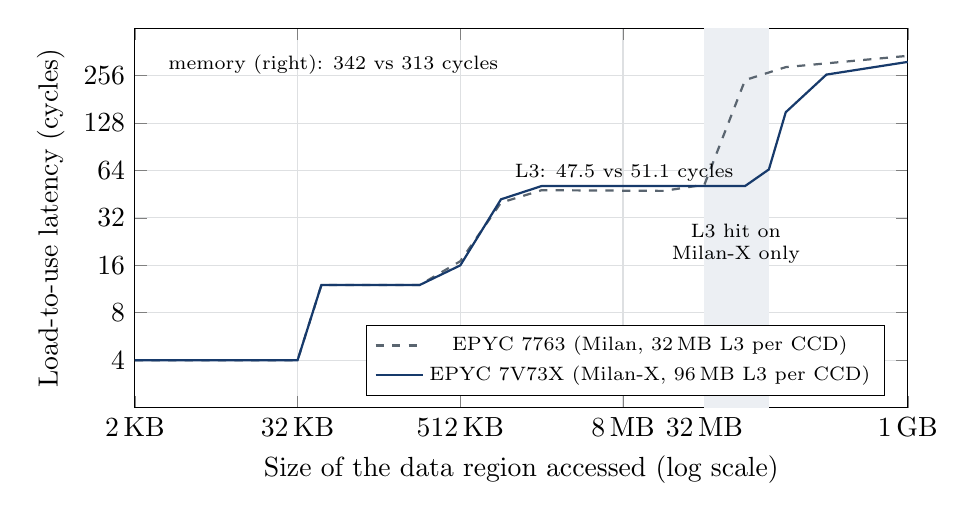
\begin{tikzpicture}
\begin{axis}[
  width=0.94\textwidth, height=6.4cm,
  xmode=log, log basis x=2, ymode=log, log basis y=2,
  xmin=2, xmax=1048576, ymin=2, ymax=512,
  xtick={2,32,512,8192,32768,1048576}, xticklabels={2\,KB,32\,KB,512\,KB,8\,MB,32\,MB,1\,GB},
  ytick={4,8,16,32,64,128,256}, yticklabels={4,8,16,32,64,128,256},
  xlabel={Size of the data region accessed (log scale)}, ylabel={Load-to-use latency (cycles)},
  legend pos=south east, legend style={font=\scriptsize},
  grid=major, grid style={draftgray!20}]
\fill[draftblue!8] (axis cs:32768,2) rectangle (axis cs:98304,512);
\addplot[draftgray,thick,dashed] coordinates {(2,4) (32,4) (48,12) (256,12) (512,17) (1024,40) (2048,48) (16384,47.5) (32768,52) (65536,240) (131072,290) (1048576,342)};
\addlegendentry{EPYC 7763 (Milan, 32\,MB L3 per CCD)}
\addplot[draftblue,thick] coordinates {(2,4) (32,4) (48,12) (256,12) (512,16) (1024,42) (2048,51) (65536,51) (98304,65) (131072,150) (262144,260) (1048576,313)};
\addlegendentry{EPYC 7V73X (Milan-X, 96\,MB L3 per CCD)}
\node[font=\scriptsize,anchor=west] at (axis cs:1100,62) {L3: 47.5 vs 51.1 cycles};
\node[font=\scriptsize,anchor=west] at (axis cs:3,300) {memory (right): 342 vs 313 cycles};
\node[font=\scriptsize,align=center] at (axis cs:56000,22) {L3 hit on\\Milan-X only};
\end{axis}
\end{tikzpicture}
\caption[Cache and memory latency of Milan and Milan-X against data size]{Cache and memory latency against data size for Milan and Milan-X, redrawn from Chips and Cheese's measurements \cite{cozmaAMDsVCacheTested2022}. The labelled values (L1 4 cycles, L2 about 12 cycles, L3 47.49 and 51.14 cycles, memory 342 and 313 cycles) are taken from the chart's own labels; the transitions between them were read by eye and are approximate. In the shaded range, from 32\,MB to beyond about 64\,MB, Milan-X still hits in its L3 while Milan already goes to memory.}
\label{fig:milanx-latency}
\end{figure}

\subsection{Lam's six workloads in detail}
\label{sec:lam-detail}
Lam's measurements are the best-controlled evidence available (\cref{sec:confounds}), so they are worth reading workload by workload. Lam tested four games, GHPC (which simulates the fire-control systems of armoured vehicles), Cyberpunk~2077, the flight simulator DCS and Call of Duty, together with libx264 video encoding and 7-Zip compression \cite{lamAMDs7950X3DZen2023}. \Cref{tab:lam-detail} collects the L3 hit rates and IPC values from Lam's charts and the misses per thousand instructions (MPKI) from the text \cite{lamAMDs7950X3DZen2023}.

\begin{table}[htbp]
  \centering
  \caption[Lam's per-CCD measurements on the Ryzen~9 7950X3D, both CCDs at 4.2\,GHz]{Lam's per-CCD measurements on the Ryzen~9 7950X3D, both CCDs at 4.2\,GHz \cite{lamAMDs7950X3DZen2023}. Hit rates and IPC read from the article's charts (IPC to two decimals); IPC gains as stated in the text where given (Call of Duty: computed from the chart; the text says ``over 19\%''); MPKI on the plain CCD as stated in the text. Lam counts L3 accesses from the L3's side, including speculative accesses and prefetches. The Cyberpunk run was limited by the graphics card, which is why Lam compares IPC rather than frame rates.}
  \label{tab:lam-detail}
  \footnotesize
  \begin{tabularx}{\textwidth}{@{}>{\raggedright\arraybackslash}X cccc c@{}}
    \toprule
    \textbf{Workload} & \textbf{L3 hit rate} & \textbf{L3 miss rate} & \textbf{IPC} & \textbf{IPC gain} & \textbf{MPKI} \\
    & plain $\to$ V-Cache & plain $\to$ V-Cache & plain $\to$ V-Cache & & plain \\
    \midrule
    Call of Duty & 46.5 $\to$ 68.7\% & 53.5 $\to$ 31.3\% & 0.71 $\to$ 0.85 & 19.7\% & not legible \\
    Cyberpunk 2077 & 46.0 $\to$ 63.7\% & 54.0 $\to$ 36.3\% & 1.26 $\to$ 1.43 & 13.5\% & 5 \\
    7-Zip & 45.8 $\to$ 59.2\% & 54.2 $\to$ 40.8\% & 1.33 $\to$ 1.46 & 9.75\% & not stated \\
    GHPC & 58.7 $\to$ 78.0\% & 41.4 $\to$ 22.0\% & 1.15 $\to$ 1.27 & 9.67\% & 5.5 \\
    libx264 & 61.6 $\to$ 71.9\% & 38.5 $\to$ 28.1\% & 1.36 $\to$ 1.43 & 4.9\% & 1.48 \\
    DCS (flight simulator) & 89.1 $\to$ 92.4\% & 10.9 $\to$ 7.6\% & about 1.7 (both) & small loss & 0.35 \\
    \bottomrule
  \end{tabularx}
\end{table}

\textbf{A summary figure.} The method of this part reports ranges rather than a single average, but a summary helps when comparing with AMD's figures. Over the five workloads with a quantified gain, the geometric mean of the IPC ratios, which is the authors' calculation and not Lam's, is $(1.049 \times 1.0967 \times 1.0975 \times 1.1349 \times 1.197)^{1/5} \approx 1.114$, an 11.4\% gain at equal clock, and the median is 9.75\%. DCS lost a little, by an amount the article does not state. Counting it as no change gives $1.114^{5/6} \approx 1.094$, so the geometric mean over all six workloads is at most 9.4\%. These six workloads were chosen by the author, four of them games, so the mean describes this sample and not software in general; the 350 Phoronix results of \cref{sec:phoronix} are the better guide to how common such gains are.

\textbf{What the hit rates say.} In every workload the V-Cache raised the L3 hit rate, by 3 to 22 percentage points, and removed between a quarter and a half of the L3 misses (from 54.2 to 40.8\% for 7-Zip, a quarter; from 41.4 to 22.0\% for GHPC, almost half). The capacity argument of \cref{sec:why-cache-capacity} predicts exactly this: tripling the L3 turns some capacity misses into hits but leaves the misses of data that does not fit even in 96\,MB, or that is touched for the first time.

\textbf{What the IPC gains say.} The ranking of gains follows the ranking of misses only loosely. DCS, with 0.35 MPKI, had almost nothing to gain and lost a little, which Lam attributes to the added L3 latency; libx264, with 1.48 MPKI, gained 4.9\%; the four miss-heavy workloads (Call of Duty, Cyberpunk, 7-Zip and GHPC, which miss on 41--54\% of their L3 accesses) gained 9.67--19.7\%. Among them, however, GHPC had the highest stated MPKI (5.5) and the largest relative fall in miss rate, yet gained less than Cyberpunk. The data allow a rough check of why, using the method of \cref{sec:tradeoff-example}. For each workload with a stated MPKI, the number of L3 accesses per thousand instructions is MPKI divided by the miss rate (for GHPC, $5.5/0.414 \approx 13.3$). The misses removed follow from the two miss rates ($5.5 - 13.3 \times 0.220 \approx 2.57$), and the cycles saved follow from the two IPC values, to which the four extra cycles on every L3 access are added back (\cref{tab:lam-per-miss}).

\begin{table}[htbp]
  \centering
  \caption[Cycles saved per removed L3 miss]{Cycles saved per removed L3 miss, derived from \cref{tab:lam-detail} with four extra cycles per L3 access (approximate; see text).}
  \label{tab:lam-per-miss}
  \small
  \begin{tabular}{@{}lccccc@{}}
    \toprule
    & \multicolumn{4}{c}{\textbf{per thousand instructions}} & \textbf{Cycles per} \\
    \cmidrule(lr){2-5}
    \textbf{Workload} & \textbf{L3 accesses} & \textbf{Misses removed} & \textbf{Cycles saved} & \textbf{Cycles added} & \textbf{removed miss} \\
    \midrule
    GHPC & 13.3 & 2.57 & 77 & 53 & about 50 \\
    Cyberpunk 2077 & 9.3 & 1.64 & 94 & 37 & about 80 \\
    libx264 & 3.85 & 0.40 & 36 & 15 & about 130 \\
    \bottomrule
  \end{tabular}
\end{table}

The pattern in \cref{tab:lam-per-miss} is that the more misses a workload has, the less each removed miss appears to be worth. The overlap of misses in \cref{sec:mlp} would produce this: a workload with many outstanding misses hides more of each one, so removing a miss saves less of its latency. Prefetches counted as misses would have the same effect (\cref{sec:tradeoff-example}). The values are therefore \emph{apparent cycles saved per counted miss}, and they inherit the caveats of \cref{sec:tradeoff-example}, including the 15\% difference in L3 accesses per instruction between the two CCDs found for DCS. The figures are approximate. The IPC values are read to two decimals, so for GHPC the chart's 1.15 and 1.27 give a 10.4\% gain against the 9.67\% in the text, which would raise its figure to about 53 cycles. The calculation also assumes that all the IPC change comes from L3 misses and latency; and each workload was measured in one scenario. The ordering, however, is not sensitive to these errors, because the three values differ by more than a factor of two.

\textbf{What else limits the gain.} Call of Duty shows that the cache is not the only bottleneck even in a miss-heavy game. Lam's breakdown of pipeline slots shows the V-Cache cutting the share of slots lost to the back end, which waits for data, from 29.7\% to 24.2\%, while the share lost to the front end, which supplies instructions, stayed at about 42--43\% \cite{lamAMDs7950X3DZen2023}. Lam concludes that most of the hit-rate gain came from data-side misses. The game's IPC of 0.85 with V-Cache is still the lowest of the six, so the 19.7\% gain is large in relative terms but leaves the core mostly waiting on instruction supply.

\textbf{At stock clocks.} In normal operation, Lam's plain CCD clocked about 7\% higher than the V-Cache CCD \cite{lamAMDs7950X3DZen2023}. If performance scaled linearly with clock, dividing each IPC ratio by 1.07 would give the net effect of choosing the V-Cache CCD: 0.98$\times$ for libx264, 1.03$\times$ for GHPC and 7-Zip, 1.06$\times$ for Cyberpunk and 1.12$\times$ for Call of Duty. Lam notes that performance does not scale linearly with clock, because memory latency does not improve with core frequency, so these values are lower bounds for the V-Cache CCD; libx264, with few misses, is the case closest to linear and the only one likely to favour the faster plain CCD. \Cref{sec:cache-clock-model} develops this trade-off into a model.

\subsection{A working-set sweep: MiniFE}
\label{sec:minife}
Domke \emph{et al.} ran the MiniFE finite-element proxy application on dual-socket Milan and Milan-X systems with the same 64 cores per socket, 280\,W TDP and 16-channel DDR4 memory, while scaling the problem from $100^3$ to $400^3$ grid points \cite{domkeLocusPerformanceQuantifying2023}. \Cref{fig:minife-sweep} shows the result: a sweep through working-set sizes of exactly the kind sketched in \cref{fig:working-set}.
\begin{itemize}
  \item At the smallest sizes ($n = 100$ and 110) Milan-X is about 10\% \emph{slower}. Both systems hold the data in L3, so the difference is probably Milan's higher base clock (2.45 against 2.20\,GHz); \cref{sec:clock-correction} tests this.
  \item From $n = 120$ the advantage rises steeply, to 3.4$\times$ at $n = 160$. In this range Milan's 512\,MiB of L3 (two sockets) no longer holds the data, while Milan-X's 1536\,MiB still does.
  \item Beyond $n = 170$ the advantage falls quickly and settles at about 1.04$\times$ from $n \approx 330$ onwards, once the data exceeds both caches.
\end{itemize}

\textbf{Inferring the working set.} The curve can be used to estimate how much data each grid point needs, with no information about MiniFE's data structures. Milan's own performance falls sharply between $n = 120$ and 130 \cite[Fig.~1]{domkeLocusPerformanceQuantifying2023}, that is, between $1.73$ and $2.20$ million points; if this is where the data outgrows 512\,MiB, each point needs about $512 \times 2^{20} / (1.73\text{ to }2.20 \times 10^6) \approx 245$--310 bytes. Milan-X's performance falls between $n = 170$ and 180, between $4.91$ and $5.83$ million points; with 1536\,MiB of L3 that gives about 275--330 bytes per point. The two independent estimates agree, which supports the reading that the speedup curve is a cache-capacity effect: at about 300 bytes per point, Milan-X's L3 holds three times as many grid points as Milan's. The estimate is approximate, because not all of the L3 holds useful data and the two sockets' caches are not perfectly shared.

\begin{figure}[htbp]
\centering
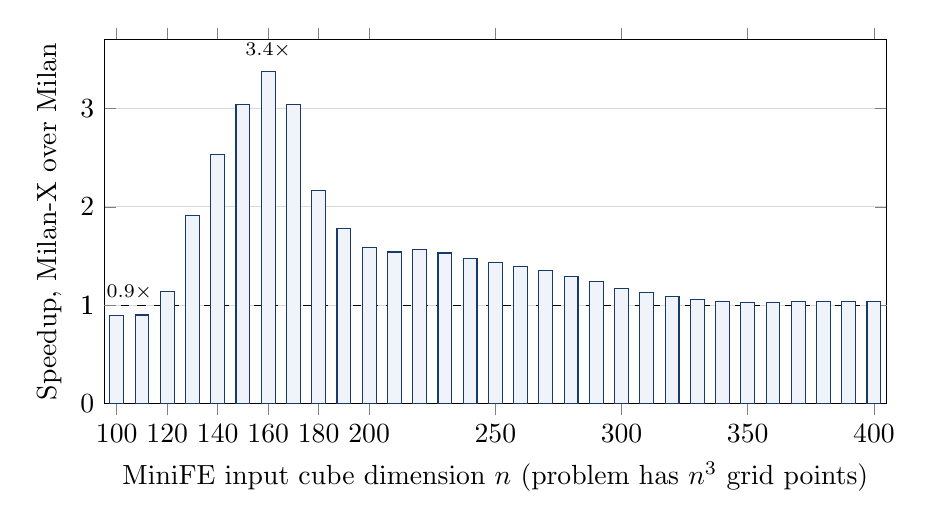
\begin{tikzpicture}
\begin{axis}[
  ybar, bar width=5pt, width=0.95\textwidth, height=6.2cm,
  ymin=0, ymax=3.7, ylabel={Speedup, Milan-X over Milan},
  xlabel={MiniFE input cube dimension $n$ (problem has $n^3$ grid points)},
  xtick={100,120,140,160,180,200,250,300,350,400}, xmin=95, xmax=405,
  ymajorgrids, grid style={draftgray!25},
  extra y ticks={1}, extra y tick style={grid style={black,dashed}}]
\addplot[fill=draftlight,draw=draftblue] coordinates {
 (100,0.89) (110,0.90) (120,1.14) (130,1.91) (140,2.53) (150,3.04) (160,3.38) (170,3.04) (180,2.17) (190,1.78)
 (200,1.59) (210,1.54) (220,1.57) (230,1.53) (240,1.47) (250,1.43) (260,1.39) (270,1.35) (280,1.29) (290,1.24)
 (300,1.17) (310,1.13) (320,1.09) (330,1.06) (340,1.04) (350,1.03) (360,1.03) (370,1.04) (380,1.04) (390,1.04) (400,1.04)};
\node[font=\scriptsize,anchor=south] at (axis cs:160,3.42) {3.4$\times$};
\node[font=\scriptsize,align=center,anchor=south] at (axis cs:105,0.95) {0.9$\times$};
\end{axis}
\end{tikzpicture}
\caption[MiniFE speed-up of Milan-X over Milan as the problem size grows]{MiniFE on a dual-socket EPYC 7773X (Milan-X, 2$\times$768\,MiB L3) against a dual-socket EPYC 7763 (Milan, 2$\times$256\,MiB L3) as the problem size grows. Values were read by eye from Domke \emph{et al.}'s figure \cite[Fig.~1]{domkeLocusPerformanceQuantifying2023} and are accurate to about $\pm 0.05$. Milan-X runs at a lower base clock (2.20 against 2.45\,GHz).}
\label{fig:minife-sweep}
\end{figure}

\subsection{OpenFOAM in detail}
\label{sec:openfoam}
Lawenda \emph{et al.}'s OpenFOAM study adds measured miss rates and clock speeds \cite{lawendaEvaluatingImpactL32025}. For the dual-socket 64-core Rome, Milan and Genoa systems, all with 256\,MB of L3 per socket, the L3 miss rate rose from about 10--15\% on the smallest motorBike meshes to about 80\% on the largest. Milan-X, with 768\,MB per socket, cut the miss rate by up to 30 percentage points on the mid-sized to large meshes. Its performance relative to Milan ranged from 0.81$\times$ to 1.54$\times$ across the eight mesh sizes: slower on some small meshes, fastest at the ``mhigh'' mesh of 6.7 million cells, and falling back to 1.24$\times$ on the largest (xhigh) mesh of 39.4 million cells, where the data exceeds even Milan-X's cache (1.22$\times$ in their Fig.~4). Expressed per core, Lawenda \emph{et al.} place Milan-X's advantage between about 15\,000 and 100\,000 cells per core. Its best utilisation came at about 14\,800 cells per core, against about 4700 for Rome and Milan. The newer generation shows the same pattern (\cref{sec:genoax}). \Cref{fig:openfoam-sweep} plots the ratios Lawenda \emph{et al.}\ label in their figure for the five larger meshes.

\begin{figure}[htbp]
\centering
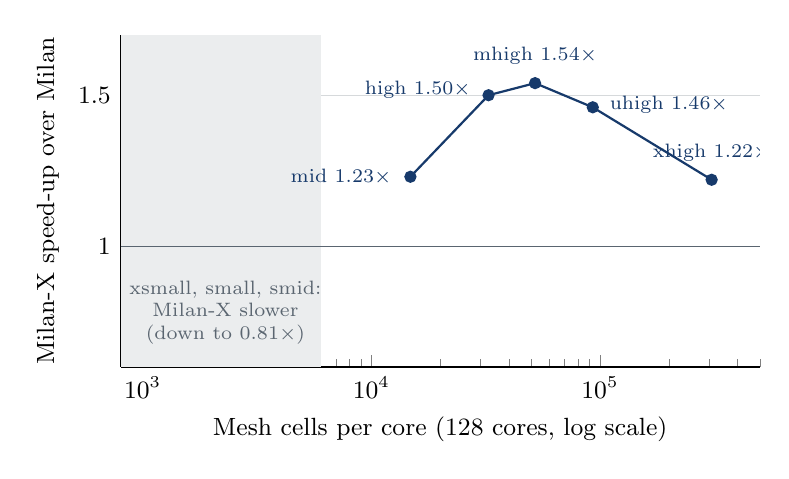
\begin{tikzpicture}
\begin{axis}[
  width=0.8\textwidth, height=5.8cm,
  xmode=log, xmin=800, xmax=500000, ymin=0.6, ymax=1.7,
  xlabel={Mesh cells per core (128 cores, log scale)}, ylabel={Milan-X speed-up over Milan},
  ymajorgrids, grid style={draftgray!25}, axis x line*=bottom, axis y line*=left,
  label style={font=\small}, tick label style={font=\small}]
\fill[draftgray!12] (axis cs:800,0.6) rectangle (axis cs:6000,1.7);
\node[font=\scriptsize,text=draftgray,align=center] at (axis cs:2300,0.78) {xsmall, small, smid:\\Milan-X slower\\(down to 0.81$\times$)};
\addplot[draftblue,thick,mark=*,mark size=1.8pt] coordinates {
  (14822,1.23) (32550,1.50) (52012,1.54) (92972,1.46) (307815,1.22)};
\node[font=\scriptsize,text=draftblue,anchor=east] at (axis cs:13500,1.23) {mid 1.23$\times$};
\node[font=\scriptsize,text=draftblue,anchor=east] at (axis cs:30000,1.52) {high 1.50$\times$};
\node[font=\scriptsize,text=draftblue,anchor=south] at (axis cs:52012,1.57) {mhigh 1.54$\times$};
\node[font=\scriptsize,text=draftblue,anchor=west] at (axis cs:100000,1.47) {uhigh 1.46$\times$};
\node[font=\scriptsize,text=draftblue,anchor=south] at (axis cs:307815,1.25) {xhigh 1.22$\times$};
\addplot[draftgray,thin] coordinates {(800,1)(500000,1)};
\end{axis}
\end{tikzpicture}
\caption[OpenFOAM speed-up of Milan-X over Milan by mesh size]{OpenFOAM motorBike: speed-up of a dual-socket EPYC~7773X (Milan-X) system over a dual-socket EPYC~7763 (Milan) system by mesh size, read from Lawenda \emph{et al.}'s Fig.~4, with cells per core from their Table~3 \cite{lawendaEvaluatingImpactL32025}. The gain peaks where the working set fits the larger L3 but not the smaller one, and falls on the largest mesh, which exceeds both. The figure labels the xhigh gain 1.22$\times$ while the article's text gives 1.24$\times$. For the three smallest meshes the figure gives no ratio; the article's Table~6 gives a lowest value of 0.81$\times$. Clocks were not fixed (\cref{tab:clock-correction}).}
\label{fig:openfoam-sweep}
\end{figure}


The study's measured clocks show the confound discussed in \cref{sec:confounds}: during the runs, Milan ran at 2.9--3.2\,GHz and Milan-X at 2.8--3.0\,GHz \cite[Table~5]{lawendaEvaluatingImpactL32025}. Milan-X's losses on the small meshes, where both systems' caches suffice, are therefore at least partly a clock effect, as in MiniFE.

\subsection{The next generation: Genoa-X}
\label{sec:genoax}
Lawenda \emph{et al.} also measured the fourth generation: dual-socket systems with the 64-core EPYC~9554 and the 96-core EPYC~9654 (Genoa) and the 96-core EPYC~9684X (Genoa-X), which adds a cache die to each of its twelve CCDs \cite{lawendaEvaluatingImpactL32025}. Their results allow three comparisons that the third-generation data cannot.

\textbf{The same pattern, a wider window.} Against the 96-core Genoa, Genoa-X ranged from 0.98$\times$ to 1.60$\times$ across the motorBike meshes, against 0.81$\times$ to 1.54$\times$ for Milan-X against Milan. As with Milan-X, it was not faster on the smaller meshes, and its largest gains came on the mid-sized to large ones. Lawenda \emph{et al.} place Genoa-X's advantage between about 10\,000 and 200\,000 cells per core, against 15\,000 to 100\,000 for Milan-X \cite{lawendaEvaluatingImpactL32025}. The two stacked products have the same L3 per core: $768/64 = 12$\,MB per core for the EPYC~7773X \cite{lawendaEvaluatingImpactL32025} and $1152/96 = 12$\,MB for the 9684X \cite{advancedmicrodevicesinc.AMDEPYC90042023}. The wider window therefore cannot come from more L3 per core, although the L2 does double, from 512\,KB to 1\,MB per core \cite{lawendaEvaluatingImpactL32025}. One candidate is memory bandwidth: Genoa has twelve channels of DDR5-4800, 460.8\,GB/s per socket or 4.8\,GB/s per core on the 96-core parts \cite{advancedmicrodevicesinc.AMDEPYC90042023}, against 204.8\,GB/s or 3.2\,GB/s per core for a 64-core Milan (\cref{sec:d2d}). The source does not test this explanation, so it remains a hypothesis.

\textbf{A smaller loss on small meshes.} Milan-X's worst case was 0.81$\times$, and \cref{sec:clock-correction} found that the measured clocks explain only part of it. Genoa-X's worst case was 0.98$\times$, a loss of 2\%. The clock table of Lawenda \emph{et al.} gives 3.4--3.5\,GHz and 3.2--3.4\,GHz for two of the fourth-generation systems, but its row labels for the Genoa family appear to be misprinted (two rows are labelled ``64-core Genoa'' and none ``Genoa X'') \cite[Table~5]{lawendaEvaluatingImpactL32025}. If those two rows are the 96-core Genoa and Genoa-X, in the order the paper uses elsewhere, Genoa-X ran about 4\% slower, and the 2\% loss is no more than its clock deficit. The reading is plausible but rests on that assumption.

\textbf{A new generation outweighs a stacked cache.} Without any stacked cache, the 64-core Genoa was 1.24--1.70$\times$ as fast as Milan-X on every mesh \cite{lawendaEvaluatingImpactL32025}, and Genoa-X was up to 2.67$\times$ as fast as Milan-X. The gain from one generation of core, memory (DDR5) and clock was larger than the gain from tripling the L3 within a generation. This is a caution against reading too much into any single factor: the stacked cache is one way to buy performance among several, and it is most valuable where the other ways run out, as \cref{sec:bandwidth-wall} argues.

\subsection{Do the independent sources agree?}
\label{sec:cross-check}
Three articles from one independent outlet, Chips and Cheese, measured the same programs or the same quantity on different generations, which allows a direct check of consistency (\cref{tab:cross-check}). Cozma compared one CCD of Milan-X with one CCD of Milan in cloud instances, estimated that Milan-X ran about 5\% slower (3.15 against 3.3\,GHz), and corrected those results for that difference \cite{cozmaDeepDivingZen2022}. Lam measured the Zen~4 7950X3D at a fixed clock \cite{lamAMDs7950X3DZen2023}.

\begin{table}[htbp]
  \centering
  \caption[Cross-check of independent results across generations]{Cross-check of independent results for the same program or quantity on different generations.}
  \label{tab:cross-check}
  \small
  \begin{tabularx}{\textwidth}{@{}l>{\raggedright\arraybackslash}X>{\raggedright\arraybackslash}X>{\raggedright\arraybackslash}p{2.3cm}@{}}
    \toprule
    \textbf{Quantity} & \textbf{Zen~3: Milan-X vs Milan, one CCD \cite{cozmaDeepDivingZen2022}} & \textbf{Zen~4: 7950X3D CCDs at 4.2\,GHz \cite{lamAMDs7950X3DZen2023}} & \textbf{Agreement} \\
    \midrule
    7-Zip & $+5\%$ measured; about $+10\%$ at equal clock (source's correction) & $+9.75\%$ IPC & close \\
    libx264 & $+5\%$ measured; about $+10\%$ at equal clock & $+4.9\%$ IPC & differs by half \\
    gem5 & $+7.6\%$ measured; about $+12.5\%$ at equal clock & not tested & --- \\
    Added L3 latency & 3--4 cycles (47.49 to 51.14 on Milan-X \cite{cozmaAMDsVCacheTested2022}) & about 4 cycles & close; also 4 on Zen~5 \cite{cozmaAMDs9800X3D2nd2024} \\
    \bottomrule
  \end{tabularx}
\end{table}

The latency cost agrees across all three generations, as \cref{sec:vcache-access} noted. The 7-Zip results also agree: about 10\% at equal clock on both Zen~3 and Zen~4. The libx264 results do not: Cozma's corrected figure is about twice Lam's. Several differences could explain this, and the sources do not allow a choice among them. Cozma's clocks are estimated and the correction assumes performance proportional to clock, which overstates the per-clock gain of a program that waits on memory (\cref{sec:clock-correction}). The two used different videos and possibly different settings. And the Zen~4 core has a 1\,MB L2 \cite{advancedmicrodevicesinc.4thGenAMD2023}, twice Zen~3's 512\,KB \cite[slide~19]{wuu2022vcache}, so more of libx264's reuse may be caught before the L3 on Zen~4, leaving less for the V-Cache to remove. The last point is a hypothesis; neither source measured Zen~3 and Zen~4 under the same conditions.

A later measurement shows the same pattern on Zen~5. In SPEC~CPU~2017, the eight-core 9800X3D ran ahead of the sixteen-core 9950X in the integer suite and almost made up its 500\,MHz clock deficit in the floating-point suite. In the floating-point suite, the two most memory-bound tests gained most, 7.5\% for 549.fotonik3d and 15\% for 554.roms \cite{cozmaAMDs9800X3D2nd2024}. With the clock deficit of about 9\% (5.2 against the 9950X's rated 5.7\,GHz), those gains imply per-clock improvements of very roughly 18--26\% for the two memory-bound tests, on the same simple correction and with the same caveat.

The cross-check shows that the mechanism is stable across generations: the latency cost is the same, and the programs that gain most are usually among those that miss most, though not always: Cozma notes that 523.xalancbmk, the most memory-bound SPEC test on Zen~5, sees little benefit from V-Cache \cite{cozmaAMDs9800X3D2nd2024}, and Lam's GHPC gained less than Cyberpunk despite more misses. The size of the gain for a given program is less stable, because it depends on the rest of the hierarchy, on the input and on how the clock is controlled. This is why \cref{sec:evidence-method} reports each result with its conditions.

\subsection{Breadth: 350 desktop results}
\label{sec:phoronix}
Phoronix compared the eight-core Ryzen~7 5800X3D and 5800X across 420 benchmarks on Linux and charted the 350 with a statistically significant difference \cite{larabelAMDRyzen72022}. Classifying each result by the colour of its bar in that chart gives the distribution in \cref{fig:phoronix-hist}. The 5800X was faster in 244 tests, but all except three of those margins were under 10\% and the median was about 4\%, consistent with its higher clocks. The 5800X3D was faster in 106 tests, with a median margin of about 11\%; 58 of its wins were 10\% or more and 12 exceeded 50\%, led by ASKAP's tConvolve gridding kernel (294\%), Zstd compression, oneDNN, CloverLeaf and OpenFOAM (68\%). Phoronix's own summary describes the 5800X winning ``a small set of tests''; the chart shows that the 5800X won more tests but by much smaller margins. The distribution is the clearest available picture of the workload dependence: for most desktop software the stacked cache costs a few percent, and for a minority it is worth tens of percent or more.

\begin{figure}[htbp]
\centering
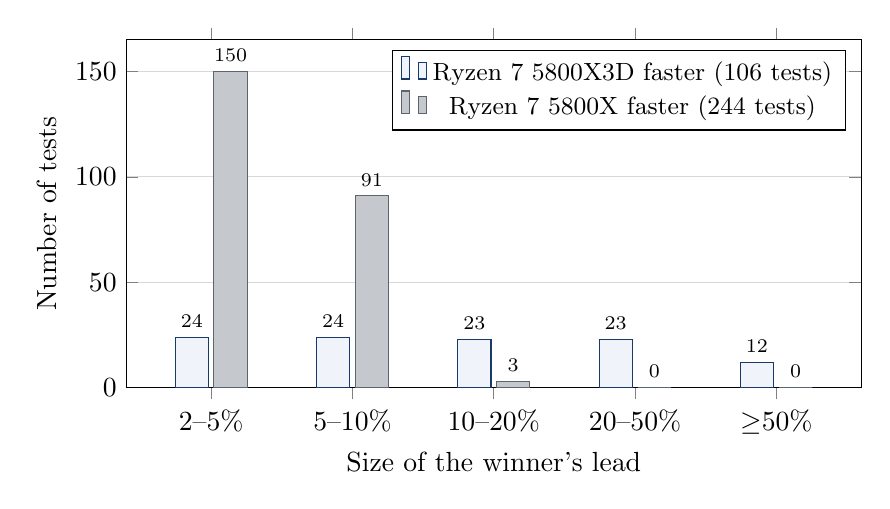
\begin{tikzpicture}
\begin{axis}[
  ybar, bar width=12pt, width=0.9\textwidth, height=6.0cm,
  ymin=0, ymax=165, ylabel={Number of tests},
  symbolic x coords={2--5\%,5--10\%,10--20\%,20--50\%,$\ge$50\%}, xtick=data,
  xlabel={Size of the winner's lead},
  legend style={font=\small,at={(0.98,0.97)},anchor=north east},
  nodes near coords, nodes near coords style={font=\scriptsize},
  ymajorgrids, grid style={draftgray!25}, enlarge x limits=0.15]
\addplot[fill=draftlight,draw=draftblue] coordinates {(2--5\%,24) (5--10\%,24) (10--20\%,23) (20--50\%,23) ($\ge$50\%,12)};
\addplot[fill=draftgray!35,draw=draftgray] coordinates {(2--5\%,150) (5--10\%,91) (10--20\%,3) (20--50\%,0) ($\ge$50\%,0)};
\legend{Ryzen~7 5800X3D faster (106 tests), Ryzen~7 5800X faster (244 tests)}
\end{axis}
\end{tikzpicture}
\caption[Distribution of Phoronix's 350 significant differences, 5800X3D against 5800X]{Distribution of the 350 statistically significant differences among Phoronix's 420 benchmarks of the Ryzen~7 5800X3D and 5800X \cite{larabelAMDRyzen72022}. The winner of each test was identified from the colour of its bar in Phoronix's comparison chart and matched to the chart's printed percentages; this classification is ours. Each bin includes its lower bound (for example, 5--10\% means at least 5\% and less than 10\%).}
\label{fig:phoronix-hist}
\end{figure}

\section{Cache-Sensitive Versus Cache-Insensitive Workloads}
\label{sec:workload-sensitivity}
The evidence sorts workloads into three groups, matching the working-set argument of \cref{sec:vcache-workloads}:
\begin{itemize}
  \item \textbf{Strongly cache-sensitive:} memory-bound HPC and engineering codes whose working sets fall between the base and stacked capacities (MiniFE, OpenFOAM at mid-sized meshes, RTL simulation) and games with high L3 miss rates. Gains range from about 10\% to more than 3$\times$ \cite{domkeLocusPerformanceQuantifying2023,lawendaEvaluatingImpactL32025,lamAMDs7950X3DZen2023}.
  \item \textbf{Mildly sensitive:} workloads with moderate miss rates, such as compression and video encoding, gain around 5--10\% at equal clock \cite{lamAMDs7950X3DZen2023,cozmaDeepDivingZen2022}, which a V-Cache part's lower clock can cancel.
  \item \textbf{Insensitive or negative:} workloads whose working sets already fit (small OpenFOAM meshes, the flight simulator in Lam's tests) or that are compute-bound gain nothing and can lose slightly from the added latency or lower clocks \cite{lawendaEvaluatingImpactL32025,lamAMDs7950X3DZen2023,larabelAMDRyzen72022}.
\end{itemize}
A useful first screen is therefore not the application type but its L3 miss rate on the base configuration: in Lam's results, the workloads with the most L3 misses gained most and those with the fewest gained least or lost \cite{lamAMDs7950X3DZen2023}. The order is not strict, because each removed miss is worth less in a workload that overlaps many misses (\cref{sec:lam-detail}).

\section{Separating Cache Effects From Other Factors}
\label{sec:confounds}

A difference in measured performance between two processors can rarely be attributed to cache size alone. Using \cref{eq:perf} and \cref{eq:amat}, the main confounding factors are:
\begin{itemize}
  \item \textbf{Clock frequency.} If the larger-cache part runs at a different frequency, $f$ in \cref{eq:perf} changes as well as IPC. Fixed-frequency comparisons, like the one AMD reports for its prototype \cite{swaminathanAdvancedPackagingEnabling2021}, remove this factor.
  \item \textbf{Core count and topology.} More cores or a different number of CCDs changes throughput and the cache available per core. AMD's headline desktop comparison sets an eight-core, single-CCD Ryzen~7 5800X3D against a twelve-core, two-CCD Ryzen~9 5900X \cite[slide~29]{wuu2022vcache}, so it mixes cache capacity with core count, CCD topology and clock speed. Its server comparison holds the core count at 16 but uses the EPYC~73F3 as the baseline, an F-series model that AMD positions for high frequency \cite{amd2022epyc7003,wuu2022vcache}.
  \item \textbf{Memory bandwidth and latency.} Memory speed, timings and the fabric clock change the miss penalty in \cref{eq:amat} and can make a larger cache appear more or less valuable.
  \item \textbf{Concurrent microarchitectural changes.} Generational comparisons mix many changes. AMD's 15\% Zen-to-Zen~2 IPC figure, for example, combines a new branch predictor, a larger op cache, wider floating-point paths and a doubled L3, among others \cite{suggs2019zen2}; it cannot be credited to the cache.
  \item \textbf{Power limits and software.} Package power limits, operating-system scheduling across CCDs, and application versions all affect results.
\end{itemize}

\Cref{fig:mindmap-confounds} arranges these factors in one figure.

\mapfigure{%
\node[mmroot] (r) {Why one processor beats another};
\node[mmbox,mmlevel1,fill=mmF9D7AF] (b0) at (0.00,3.60) {Clock frequency};
\draw[mmbig] (r) -- (b0);
\node[mmlevel2,mmbox,fill=mmDCCFF6] (b0c0) at (-1.52,5.35) {V-Cache parts clock lower};
\draw[mmsmall] (b0.north) to[out=90,in=-90] (b0c0.south);
\node[mmlevel2,mmbox,fill=mmDCCFF6] (b0c1) at (1.52,5.35) {Fix the clock or correct for it};
\draw[mmsmall] (b0.north) to[out=90,in=-90] (b0c1.south);
\node[mmbox,mmlevel1,fill=mmCFE7E1] (b1) at (4.47,1.36) {Cores and topology};
\draw[mmbig] (r) -- (b1);
\node[mmlevel2,mmbox,fill=mmF9D7AF] (b1c0) at (8.07,2.08) {8-core 5800X3D vs 12-core 5900X};
\draw[mmsmall] (b1.east) to[out=0,in=180] (b1c0.west);
\node[mmlevel2,mmbox,fill=mmF9D7AF] (b1c1) at (8.07,0.63) {Cache per core};
\draw[mmsmall] (b1.east) to[out=0,in=180] (b1c1.west);
\node[mmbox,mmlevel1,fill=mmCFE0F4] (b2) at (2.76,-3.56) {Memory};
\draw[mmbig] (r) -- (b2);
\node[mmlevel2,mmbox,fill=mmF9D7AF] (b2c0) at (6.36,-2.83) {Speed and timings};
\draw[mmsmall] (b2.east) to[out=0,in=180] (b2c0.west);
\node[mmlevel2,mmbox,fill=mmF9D7AF] (b2c1) at (6.36,-4.28) {Fabric clock};
\draw[mmsmall] (b2.east) to[out=0,in=180] (b2c1.west);
\node[mmbox,mmlevel1,fill=mmF4AAA2] (b3) at (-2.76,-3.56) {Core design};
\draw[mmbig] (r) -- (b3);
\node[mmlevel2,mmbox,fill=mmCFE7E1] (b3c0) at (-6.36,-2.83) {Many changes at once};
\draw[mmsmall] (b3.west) to[out=180,in=0] (b3c0.east);
\node[mmlevel2,mmbox,fill=mmCFE7E1] (b3c1) at (-6.36,-4.28) {Zen to Zen~2: 15\% IPC};
\draw[mmsmall] (b3.west) to[out=180,in=0] (b3c1.east);
\node[mmoval,mmlevel1,fill=mmDCCFF6] (b4) at (-4.47,1.36) {Power and software};
\draw[mmbig] (r) -- (b4);
\node[mmlevel2,mmbox,fill=mmF4C2BB] (b4c0) at (-8.07,2.08) {Power limits};
\draw[mmsmall] (b4.west) to[out=180,in=0] (b4c0.east);
\node[mmlevel2,mmbox,fill=mmF4C2BB] (b4c1) at (-8.07,0.63) {Scheduling, versions};
\draw[mmsmall] (b4.west) to[out=180,in=0] (b4c1.east);
}{[Overview of the confounding factors of \cref{sec:confounds}]{Overview of the confounding factors of \cref{sec:confounds}. A difference in measured performance can be credited to the cache only when the comparison controls each branch (\cref{tab:confound-grid}).}}{fig:mindmap-confounds}

\Cref{tab:confound-grid} applies this checklist to the comparisons available so far. None of AMD's published product comparisons controls every factor. The fixed-frequency prototype comparison controls clock speed and core count but does not state the memory configuration, and the server comparison controls core count but not frequency. The independent comparisons are graded the same way below the line.

\begin{table}[htbp]
  \centering
  \caption[Which confounding factors each available comparison controls]{Which confounding factors each available comparison controls (\checkmark{} = controlled, $\times$ = not controlled, $\sim$ = estimated and normalised, ? = not stated; AMD-reported rows above the line, independent below).}
  \label{tab:confound-grid}
  \small
  \begin{tabular}{@{}p{5.6cm}cccc@{}}
    \toprule
    \textbf{Comparison} & \textbf{Clock} & \textbf{Cores} & \textbf{Memory} & \textbf{Same core design} \\
    \midrule
    12-core 3D prototype vs Ryzen~9 5900X, fixed frequency \cite{swaminathanAdvancedPackagingEnabling2021} & \checkmark & \checkmark & ? & \checkmark \\
    Ryzen~7 5800X3D vs Ryzen~9 5900X \cite[slides~29, 35]{wuu2022vcache} & $\times$ & $\times$ & \checkmark & \checkmark \\
    16-core EPYC with V-Cache vs EPYC~73F3 \cite[slides~31, 35]{wuu2022vcache} & $\times$ & \checkmark & ? & \checkmark \\
    Zen to Zen~2 IPC \cite{suggs2019zen2} & ? & ? & ? & $\times$ \\
    Zen~2 to Zen~3 IPC, 3800XT vs 5800X at 4\,GHz \cite{advancedmicrodevicesinc.AMDLaunchesAMD2020} & \checkmark & \checkmark & \checkmark & $\times$ \\
    \midrule
    7950X3D V-Cache CCD vs plain CCD, both at 4.2\,GHz \cite{lamAMDs7950X3DZen2023} & \checkmark & \checkmark & \checkmark & \checkmark \\
    EPYC 7773X vs 7763 \cite{lawendaEvaluatingImpactL32025,domkeLocusPerformanceQuantifying2023} & $\times$ & \checkmark & \checkmark & \checkmark \\
    Milan-X vs Milan, one CCD \cite{cozmaDeepDivingZen2022} & $\sim$ & \checkmark & ? & \checkmark \\
    Ryzen~7 5800X3D vs 5800X \cite{larabelAMDRyzen72022} & $\times$ & \checkmark & ? & \checkmark \\
    Ryzen~7 5800X vs 3700X \cite{waltonAMDRyzen72020} & $\times$ & \checkmark & \checkmark & $\times$ \\
    \bottomrule
  \end{tabular}
\end{table}

The prototype comparison holds both clock (4.0\,GHz) and core count (12) constant but does not state the memory configuration \cite[slide~19]{swaminathanAdvancedPackagingEnabling2021}. Among the independent results, Lam's per-CCD measurements control every listed factor, which makes them the strongest available evidence for the effect of the stacked cache itself \cite{lamAMDs7950X3DZen2023}.

\subsection{Correcting for clock speed}
\label{sec:clock-correction}
Where clocks were not fixed, a rough correction is possible if the clocks during the test are known. If performance scaled linearly with frequency, dividing a measured speedup by the ratio of clock speeds would give the per-clock effect. Memory-bound code does not scale linearly, because memory latency in nanoseconds does not improve with core clock, so the true per-clock effect lies between the raw ratio and the corrected one. \Cref{tab:clock-correction} applies this to the comparisons whose clocks were measured or stated.

\begin{table}[htbp]
  \centering
  \caption[Speedups bounded by a clock correction]{Speedups bounded by a clock correction (corrected = measured $\div$ clock ratio).}
  \label{tab:clock-correction}
  \small
  \begin{tabularx}{\textwidth}{@{}>{\raggedright\arraybackslash}X>{\raggedright\arraybackslash}p{3.2cm}cc@{}}
    \toprule
    \textbf{Comparison} & \textbf{Clock ratio (V-Cache / plain)} & \textbf{Measured} & \textbf{Clock-corrected} \\
    \midrule
    OpenFOAM, best mesh \cite{lawendaEvaluatingImpactL32025} & $2.9/3.05 \approx 0.95$ (midpoints of measured ranges) & 1.54$\times$ & 1.62$\times$ \\
    OpenFOAM, worst mesh \cite{lawendaEvaluatingImpactL32025} & $\approx 0.95$ & 0.81$\times$ & 0.85$\times$ \\
    gem5, one CCD \cite{cozmaDeepDivingZen2022} & $3.15/3.3 \approx 0.95$ (estimated) & 1.076$\times$ & 1.13$\times$ \\
    MiniFE, smallest input \cite{domkeLocusPerformanceQuantifying2023} & $2.20/2.45 \approx 0.90$ (base clocks) & 0.89$\times$ & 0.99$\times$ \\
    \bottomrule
  \end{tabularx}
\end{table}
\Cref{fig:clock-correction} plots each comparison before and after the correction, which shows which comparisons reach parity once clock is accounted for (MiniFE's smallest input) and which stay below it (OpenFOAM's worst mesh).

\begin{figure}[htbp]
\centering
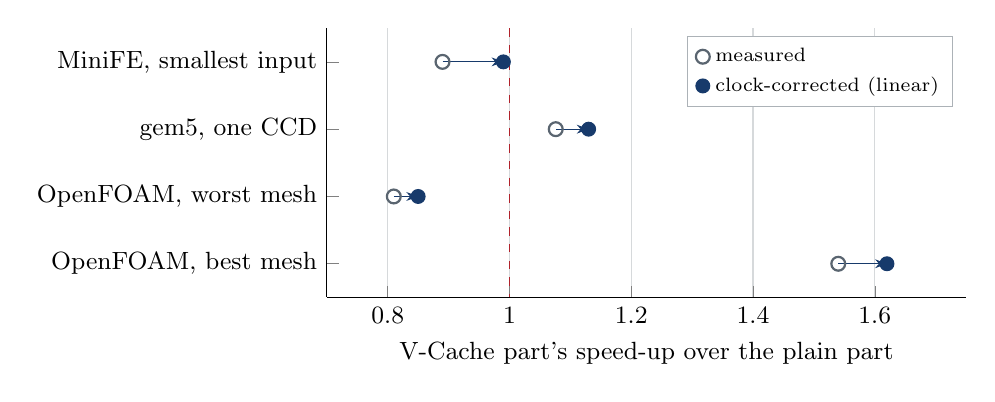
\begin{tikzpicture}
\begin{axis}[
  width=0.8\textwidth, height=5.0cm,
  xmin=0.7, xmax=1.75, ymin=0.5, ymax=4.5,
  ytick={1,2,3,4}, yticklabels={MiniFE{,} smallest input,gem5{,} one CCD,OpenFOAM{,} worst mesh,OpenFOAM{,} best mesh},
  y dir=reverse, xlabel={V-Cache part's speed-up over the plain part},
  xmajorgrids, grid style={draftgray!25}, axis x line*=bottom, axis y line*=left,
  legend style={font=\scriptsize,draw=draftgray!50,at={(0.98,0.97)},anchor=north east}, legend cell align=left,
  label style={font=\small}, tick label style={font=\small}]
\addplot[only marks,mark=o,mark size=2.5pt,draftgray,thick] coordinates {(0.89,1) (1.076,2) (0.81,3) (1.54,4)};
\addlegendentry{measured}
\addplot[only marks,mark=*,mark size=2.5pt,draftblue] coordinates {(0.99,1) (1.13,2) (0.85,3) (1.62,4)};
\addlegendentry{clock-corrected (linear)}
\foreach \a/\b/\y in {0.89/0.99/1,1.076/1.13/2,0.81/0.85/3,1.54/1.62/4}
  {\edef\tmp{\noexpand\draw[-{Stealth[length=1.5mm]},draftblue] (axis cs:\a,\y) -- (axis cs:\b,\y);}\tmp}
\draw[todored,dashed] (axis cs:1,0.5) -- (axis cs:1,4.5);
\end{axis}
\end{tikzpicture}
\caption[Comparisons before and after a linear clock correction]{The comparisons of \cref{tab:clock-correction} before and after a linear clock correction. The correction moves every point to the right, because the V-Cache part ran at a lower clock in each test; MiniFE's smallest input moves to parity, while OpenFOAM's worst mesh stays clearly below it. The true per-clock effect lies between the two markers, since memory-bound code does not speed up in proportion to clock. Sources: \cite{lawendaEvaluatingImpactL32025,cozmaDeepDivingZen2022,domkeLocusPerformanceQuantifying2023}.}
\label{fig:clock-correction}
\end{figure}


The correction changes the picture in two ways. For MiniFE's smallest input the whole 11\% loss disappears, which supports the reading that Milan-X loses there only because of its clock. For OpenFOAM's worst mesh a loss of about 15\% remains even after correction, so the clock alone does not explain it; Lawenda \emph{et al.} do not analyse that case, and the four extra cycles of L3 latency cannot account for so large a difference on their own. This is a question the published evidence leaves open. Because base clocks and measured ranges are crude stand-ins for the actual frequency during each run, the corrected values are indicative only.

\section{Cache Against Clock}
\label{sec:cache-against-clock}
In the first two generations the V-Cache parts clock lower than their plain counterparts (\cref{sec:confounds}), so whether the stacked cache pays off depends on how its gain at equal clock compares with the clock it gives up. This section works it through for the Ryzen~9 7950X3D with Lam's per-CCD measurements (\cref{sec:lam-detail}), first with a linear rule and then with a model in which memory time does not shrink with clock.

\subsection{Cache against clock on one chip}
\label{sec:cache-vs-clock}
The Ryzen~9 7950X3D makes the trade-off concrete, because its two CCDs differ only in the stacked cache and in clock speed: the plain CCD runs about 7\% faster \cite{lamAMDs7950X3DZen2023}. If performance scaled linearly with clock, the V-Cache CCD would win whenever its IPC gain at equal clock exceeded 7\%. \Cref{tab:cache-vs-clock} applies this rule to Lam's fixed-clock measurements.

\begin{table}[htbp]
  \centering
  \caption[IPC gain of the V-Cache CCD against the clock gap]{IPC gain of the V-Cache CCD at equal clock \cite{lamAMDs7950X3DZen2023} against the plain CCD's 7\% clock advantage (net $= (1 + \text{gain})/1.07 - 1$).}
  \label{tab:cache-vs-clock}
  \small
  \begin{tabular}{@{}lccc@{}}
    \toprule
    \textbf{Workload} & \textbf{IPC gain at 4.2\,GHz} & \textbf{Net, with plain CCD 7\% faster} & \textbf{Better CCD} \\
    \midrule
    libx264 & $+4.9\%$ & $-2.0\%$ & plain \\
    GHPC & $+9.7\%$ & $+2.5\%$ & V-Cache \\
    7-Zip & $+9.8\%$ & $+2.6\%$ & V-Cache \\
    Cyberpunk~2077$^{a}$ & $+13.5\%$ & $+6.1\%$ & V-Cache \\
    Call of Duty & $>+19\%$ & $>+11\%$ & V-Cache \\
    \bottomrule
  \end{tabular}
  \par\smallskip\footnotesize $^{a}$\,Lam's Cyberpunk~2077 run was limited by the graphics card, so the IPC gain did not appear as frame rate (0.5\,FPS) \cite{lamAMDs7950X3DZen2023}.
\end{table}

The linear rule overstates the plain CCD's advantage, because memory-bound programs do not speed up in proportion to clock; Lam makes this point for libx264, expecting the two CCDs to come close \cite{lamAMDs7950X3DZen2023}. The table's net values are therefore conservative for the V-Cache CCD. Even so, the result shows why AMD placed ordinary applications on the higher-clocked CCD by default, and why the choice still depends on the program \cite{lamAMDs7950X3DZen2023}.

\subsection{Refining the rule: memory time does not shrink with clock}
\label{sec:cache-clock-model}
The linear rule\index{break-even (cache against clock)} treats every cycle as if it shrank in proportion to clock frequency. A memory access does not: its latency is set mainly by the DRAM and by the path through the I/O die, and is roughly fixed in nanoseconds (\cref{sec:clock-correction}). Splitting the time per thousand instructions into a part that scales with clock and a part that does not gives
\begin{equation}
  T(f) \;=\; \frac{C + A\,\Delta t_{\mathrm{L3}}}{f} \;+\; (M - \Delta M)\,s,
  \label{eq:cache-clock-model}
\end{equation}
where $C$ is the number of cycles per thousand instructions not spent waiting for memory, and $A$ and $M$ are the L3 accesses and L3 misses per thousand instructions on the plain CCD. $\Delta t_{\mathrm{L3}}$ is the added L3 latency (zero on the plain CCD, four cycles on the stacked one), $\Delta M$ is the number of misses the larger cache removes, and $s$ is the effective stall per miss in nanoseconds. \Cref{eq:cache-clock-model} combines \cref{eq:perf,eq:vcache-tradeoff}; the only new assumption is that $s$ does not depend on the core clock.

\Cref{app:cache-clock} calibrates the model on Lam's libx264 run ($C \approx 543$ cycles, $s \approx 31$\,ns, clocks of 4.8 and 5.15\,GHz) and tabulates the result in \cref{tab:cache-clock-model}; at equal clocks it gives a 5.2\% gain, against 5.1\% from Lam's chart IPCs and the 4.9\% Lam states.

\begin{figure}[htbp]
\centering
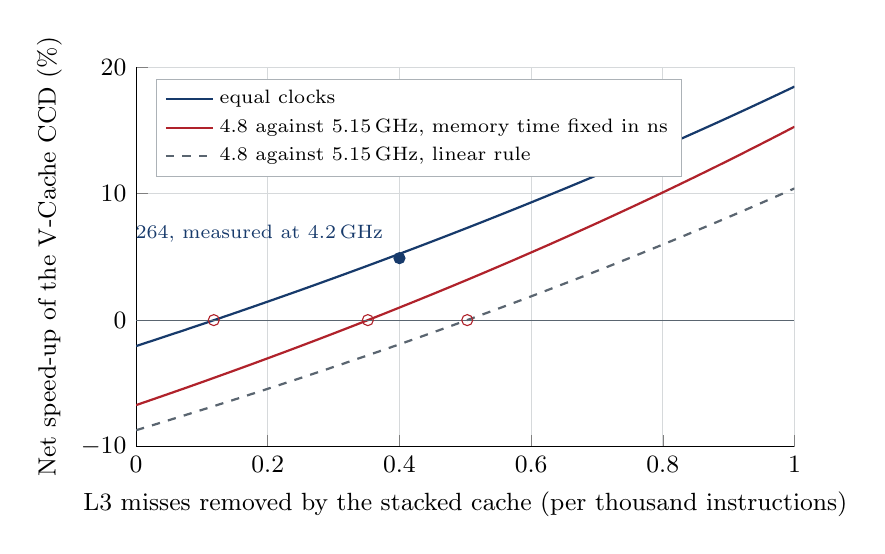
\begin{tikzpicture}
\begin{axis}[
  width=0.82\textwidth, height=6.4cm,
  xmin=0, xmax=1.0, ymin=-10, ymax=20,
  xlabel={L3 misses removed by the stacked cache (per thousand instructions)},
  ylabel={Net speed-up of the V-Cache CCD (\%)},
  xmajorgrids, ymajorgrids, grid style={draftgray!25},
  axis x line*=bottom, axis y line*=left,
  legend pos=north west, legend cell align=left, legend style={font=\scriptsize,draw=draftgray!50,fill=white},
  label style={font=\small}, tick label style={font=\small}]
\addplot[draftblue,thick,domain=0:1,samples=41] {100*(735.29/(558.29+(1.48-x)*130)-1)};
\addlegendentry{equal clocks}
\addplot[todored,thick,domain=0:1,samples=41] {100*((542.89/5.15+1.48*30.952)/(558.29/4.8+(1.48-x)*30.952)-1)};
\addlegendentry{4.8 against 5.15\,GHz, memory time fixed in ns}
\addplot[draftgray,thick,dashed,domain=0:1,samples=41] {100*((735.29/(558.29+(1.48-x)*130))/1.0729-1)};
\addlegendentry{4.8 against 5.15\,GHz, linear rule}
\addplot[draftgray,thin] coordinates {(0,0) (1,0)};
\addplot[only marks,mark=*,mark size=2pt,draftblue] coordinates {(0.40,4.9)};
\node[font=\scriptsize,anchor=south east,text=draftblue] at (axis cs:0.39,5.4) {libx264, measured at 4.2\,GHz};
\addplot[only marks,mark=o,mark size=2pt,todored] coordinates {(0.352,0) (0.118,0) (0.503,0)};
\end{axis}
\end{tikzpicture}
\caption[Cache against clock for the libx264 profile]{Cache against clock for the libx264 profile of \cref{sec:tradeoff-example}, from \cref{eq:cache-clock-model}. Open circles mark the break-even points: about 0.12 misses removed per thousand instructions at equal clocks, 0.35 with the measured clock gap if memory time is fixed in nanoseconds, and 0.50 under the linear rule. Model calibrated on Lam's fixed-clock measurements \cite{lamAMDs7950X3DZen2023}; clocks are those Lam measured under an all-core L3-sized load, not during libx264 itself.}
\label{fig:cache-clock-model}
\end{figure}

First, \cref{tab:cache-clock-model} and \cref{fig:cache-clock-model} show that the clock gap roughly triples the number of misses the stacked cache must remove to break even, from about 0.12 per thousand instructions at equal clocks of 4.2\,GHz to about 0.35, so the clock penalty matters about twice as much as the four cycles of added latency. The factor depends on the clock at which the equal-clock case is taken: at equal clocks of 4.8\,GHz the break-even would be about 0.10, and at 5.15\,GHz also about 0.10, so the factor lies between about three and three and a half. Second, the linear rule exaggerates the penalty: for libx264 it predicts a 1.9\% loss, with the model's 5.2\% and the measured 1.073 (\cref{tab:cache-vs-clock} gives 2.0\% from Lam's 4.9\% and a rounded 1.07). The refined model instead predicts a 1.0\% gain, because about 30\% of the plain CCD's time at 5.15\,GHz (26\% at the 4.2\,GHz calibration point) goes to memory stalls that a faster clock does not shorten. Lam's expectation that the two CCDs would come close on this program \cite{lamAMDs7950X3DZen2023} is what the refined model gives. Third, with no misses removed the V-Cache CCD loses 6.7\%, which is the cost a cache-insensitive program pays for running on it. The model is calibrated on one program and assumes that the clocks and the stall per miss carry over, so its numbers are illustrative; its value is in showing which quantities decide the outcome: the misses removed, the share of time spent in memory, and the clock gap.

\section{Simulation}
\label{sec:sim-study}
The published comparisons of this part never change only one thing. Even Lam's per-CCD measurements, the best controlled of them, cover six workloads on one processor (\cref{sec:lam-detail}), and every other comparison also changes the clock, the core count or the generation (\cref{tab:confound-grid}). A simulation can hold everything fixed and change one factor at a time. This section uses the group's cache-hierarchy model for that purpose. Its results are \emph{model outputs}, not measurements. Several of its inputs are fitted to the very measurements it is set beside, and several of its results follow from its synthetic workloads by construction, so the model \emph{illustrates} the mechanisms of the earlier sections in isolation; it does not confirm them independently. Each subsection says which of its agreements are built in and which are not. One comparison, with the group's own Ryzen~5 5600X, uses data the model was not built from; S0 sets out what it can and cannot show (\cref{sec:sim-calibration}).

\subsection{The model and how the experiments are run}
The model is trace-driven and functional. It follows every memory access through private L1 and L2 caches, one or more shared L3s, an optional L4 and DRAM, with a directory for coherence, and charges each access the latency of the level that served it (\cref{app:sim-setup}). It has no pipeline, so it does not predict IPC. Instead, an \emph{overlap factor} multiplies the part of every latency beyond an L2 hit, standing for the share of a miss that an out-of-order core cannot hide (\cref{sec:mlp}). The model therefore reports two averages: the \emph{raw} latency per access, which is what a latency sweep measures, and the \emph{exposed} latency per access after the overlap factor, which the experiments compare unless a caption says otherwise. The default parameters are the measured Zen~3 latencies and AMD's published figures listed in \cref{tab:sim-parameters}; the inputs that are assumptions are labelled as such there and where they are used. Every point is the mean of five runs with different random seeds, each with a warm-up and $10^6$ measured accesses ($2.5 \times 10^5$ per thread in S6). For every plotted quantity the spread between seeds was below 1\% of the mean, too small to show in the figures; for the miss counts stored alongside, it was at most 1.4\%. The CSV files on GitHub (\cref{app:sim-setup}) give the minimum and maximum for each point. \Cref{tab:sim-plan} lists the seven experiments.

\begin{table}[htbp]
  \centering
  \caption[The simulation experiments]{The simulation experiments, the factor each one changes, and what each is compared with. S0, S3 and S4 are compared with measurements their inputs are fitted to, except for the 5600X check in S0; S1 is compared in shape only.}
  \label{tab:sim-plan}
  \small
  \begin{tabularx}{\textwidth}{@{}l>{\raggedright\arraybackslash}p{3.6cm}>{\raggedright\arraybackslash}X>{\raggedright\arraybackslash}p{3.3cm}@{}}
    \toprule
    & \textbf{Question} & \textbf{Factor changed (all else equal)} & \textbf{Compared with} \\
    \midrule
    S0 & What the calibration fixes, and how close the model is to hardware & L3 size, 32 against 96\,MB; overlap factor & Milan and Milan-X latency sweep; Lam's three workloads; the group's Ryzen~5 5600X (not fitted) \\
    S1 & Where does a larger L3 help? (RQ4) & L3 size, across working sets & MiniFE sweep \\
    S2 & Stacked, planar or beside? (RQ3) & Arrangement and latency of the extra capacity & --- (no such products exist) \\
    S3 & Cache against clock & Clock gap, 0 to 10\% & Lam's 7950X3D; \cref{sec:cache-clock-model} \\
    S4 & What does the split cost? (RQ2) & Two dies or one; cost of the hop & Reguly's core-to-core test \\
    S5 & Zen~2 to Zen~3 & L3 organisation, then L3 latency & --- \\
    S6 & When does bandwidth bind? & Number of streaming threads & \cref{sec:bandwidth-wall} \\
    \bottomrule
  \end{tabularx}
\end{table}

\subsection{S0: What the calibration fixes, and how the model compares with hardware}
\label{sec:sim-calibration}
\Cref{fig:sim-latency} runs the model as a latency sweep, with random accesses and no overlap, and sets it beside Chips and Cheese's Milan and Milan-X curves. The model's L3 plateaus, 46.4 and 50.8 cycles, match the measured 47.49 and 51.14, and its latency at 1\,GB, 334 and 319 cycles, lies near the measured 342 and 313 \cite{cozmaAMDsVCacheTested2022}. Neither match is a test. The plateaus are inputs, and the 1\,GB values follow from the inputs (47 or 51 cycles plus 74\,ns at 4\,GHz, the 74\,ns measured on a different Zen~3 chip). The two pairs also differ for different reasons: the model's 1\,GB values differ because the larger L3 still holds a small fraction of the data, whereas the measured ones were taken on two instances whose clocks differed, Cozma noting that the Milan-X instance boosted higher.

\begin{figure}[htbp]
\centering
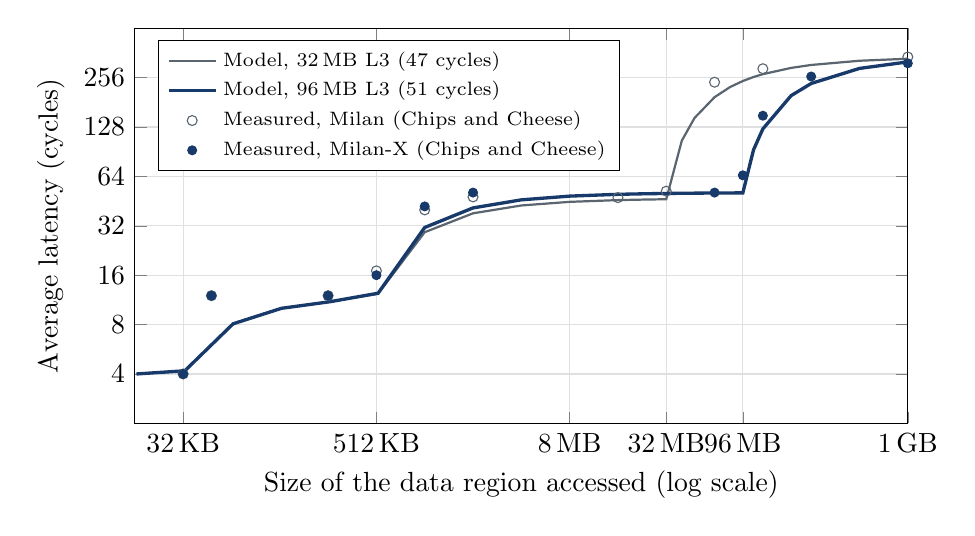
\begin{tikzpicture}
\begin{axis}[
  width=0.94\textwidth, height=6.6cm,
  xmode=log, log basis x=2, ymode=log, log basis y=2,
  xmin=16, xmax=1048576, ymin=2, ymax=512,
  xtick={32,512,8192,32768,98304,1048576}, xticklabels={32\,KB,512\,KB,8\,MB,32\,MB,96\,MB,1\,GB},
  ytick={4,8,16,32,64,128,256}, yticklabels={4,8,16,32,64,128,256},
  xlabel={Size of the data region accessed (log scale)}, ylabel={Average latency (cycles)},
  legend pos=north west, legend style={font=\scriptsize}, legend cell align=left,
  grid=major, grid style={draftgray!20}]
\addplot[draftgray,thick] coordinates {(16.384,4) (32.768,4.183) (65.536,8.089) (131.072,10.05) (262.144,11.02) (524.288,12.33) (1024,29.25) (2048,38.13) (4096,42.56) (8192,44.78) (16384,45.89) (24576,46.26) (32768,46.45) (40960,105.7) (49152,145.3) (65536,194.6) (81920,224.4) (98304,244.1) (114688,258.2) (131072,268.8) (196608,293.4) (262144,305.8) (524288,324.4) (1.04858e+06,333.7)};
\addlegendentry{Model, 32\,MB L3 (47 cycles)}
\addplot[draftblue,very thick] coordinates {(16.384,4) (32.768,4.183) (65.536,8.089) (131.072,10.05) (262.144,11.02) (524.288,12.42) (1024,31.25) (2048,41.13) (4096,46.06) (8192,48.53) (16384,49.77) (24576,50.17) (32768,50.38) (40960,50.51) (49152,50.59) (65536,50.69) (81920,50.75) (98304,50.79) (114688,93.05) (131072,124.7) (196608,198.9) (262144,235.8) (524288,291.3) (1.04858e+06,319.1)};
\addlegendentry{Model, 96\,MB L3 (51 cycles)}
\addplot[draftgray,only marks,mark=o,mark size=1.8pt] coordinates {(32,4) (48,12) (256,12) (512,17) (1024,40) (2048,48) (16384,47.5) (32768,52) (65536,240) (131072,290) (1048576,342)};
\addlegendentry{Measured, Milan (Chips and Cheese)}
\addplot[draftblue,only marks,mark=*,mark size=1.6pt] coordinates {(32,4) (48,12) (256,12) (512,16) (1024,42) (2048,51) (65536,51) (98304,65) (131072,150) (262144,260) (1048576,313)};
\addlegendentry{Measured, Milan-X (Chips and Cheese)}
\end{axis}
\end{tikzpicture}
\caption[S0: simulated latency sweep against Milan and Milan-X]{S0: the model's raw average latency (no overlap) for random accesses to a region of growing size (lines; mean of five seeds, spread smaller than the line width) against the latency sweep Chips and Cheese measured on Milan and Milan-X (points, read from \cref{fig:milanx-latency}) \cite{cozmaAMDsVCacheTested2022}. The level latencies are inputs, so their match is expected. The shape between them is not: the model's L3 stays flat up to its full capacity, whereas the measured curves rise earlier.}
\label{fig:sim-latency}
\end{figure}

\textbf{A comparison with the group's Ryzen~5 5600X.} The comparison with Milan cannot test the model, because its inputs come from the same kind of measurement. The group's own Ryzen~5 5600X provides data the model was not built from. It has one CCD with the same 32\,MB Zen~3 L3, and its latency was measured at the machine's own 4.61\,GHz with the kit described in \cref{app:5600x}, whose programs and raw results are on GitHub. \Cref{fig:m5600x-latency} sets the two side by side. The model's cache capacities and level latencies are inputs, so on each plateau its output is its input: the comparison there shows how close another Zen~3 chip's published latencies are to this one's, not how good the model is. The L1 and L2 latencies, 4 and 12 cycles, agree with the measured 4.0 and 12.1 cycles; the other two inputs differ by about 20\% or less. The measured L3 plateau is 51--55 cycles against the assumed 47, close to the about 53 cycles reported for the Ryzen~7 5800X (\cref{tab:cezanne-vermeer}), and the latency at 1\,GB is 98.6\,ns against the model's 82\,ns, a difference consistent with different memory and with the virtual machine (Windows Subsystem for Linux, WSL2) in which the measurements ran. The model's own behaviour, how hits and misses mix as a cache fills, is exercised only between the plateaus, and there the unfitted model differs from the measurement by up to 2.4 times (at 32\,MB). Fitting the L3 and memory latencies to this machine, 54 cycles and 90\,ns beyond the L3 (against the default 74\,ns), is a calibration: it aligns the plateaus and the 1\,GB value by construction (within 5\% and 1\%). It does not remove the differences near the capacity edges, which remain 1.2--2.1 times between 19 and 38\,MB and 1.1--1.3 times between 45 and 108\,MB. The comparison therefore shows two things: the published Zen~3 latencies the model uses are within about a fifth of this machine's, and close to each cache's capacity the model's latency is too low.

\begin{figure}[htbp]
\centering
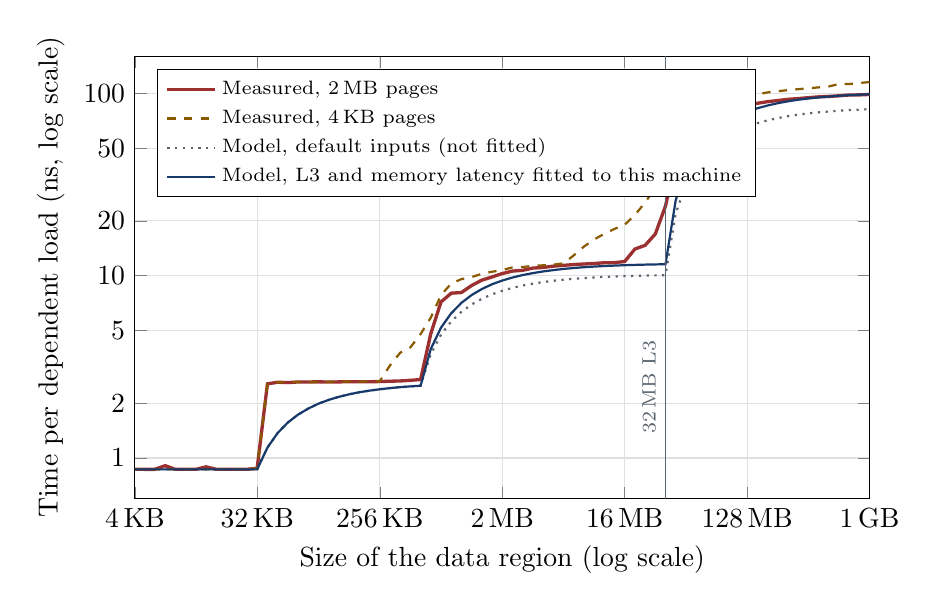
\begin{tikzpicture}
\begin{axis}[
  width=0.9\textwidth, height=7.2cm,
  xmode=log, log basis x=2, xmin=0.00390625, xmax=1024, ymode=log, ymin=0.6, ymax=160,
  ytick={1,2,5,10,20,50,100}, yticklabels={1,2,5,10,20,50,100},
  xtick={0.00390625,0.03125,0.25,2,16,128,1024}, xticklabels={4\,KB,32\,KB,256\,KB,2\,MB,16\,MB,128\,MB,1\,GB},
  xlabel={Size of the data region (log scale)}, ylabel={Time per dependent load (ns, log scale)},
  legend pos=north west, legend style={font=\scriptsize}, legend cell align=left,
  grid=major, grid style={draftgray!20}]
\addplot[mmred,very thick] coordinates {(0.003906,0.868) (0.004687,0.867) (0.005469,0.867) (0.006543,0.908) (0.007715,0.869) (0.009277,0.868) (0.01104,0.868) (0.01309,0.895) (0.01553,0.868) (0.01855,0.868) (0.02207,0.868) (0.02627,0.868) (0.03115,0.878) (0.03711,2.551) (0.04414,2.605) (0.05254,2.593) (0.0624,2.614) (0.07432,2.614) (0.08838,2.618) (0.1051,2.612) (0.1249,2.616) (0.1486,2.623) (0.1768,2.623) (0.2102,2.622) (0.2499,2.627) (0.2973,2.638) (0.3535,2.647) (0.4204,2.669) (0.4999,2.695) (0.5945,4.808) (0.7071,7.178) (0.8409,8.019) (0.9999,8.085) (1.189,8.834) (1.414,9.452) (1.682,9.839) (2,10.27) (2.378,10.6) (2.828,10.7) (3.363,11.01) (4,11.09) (4.757,11.28) (5.657,11.39) (6.727,11.51) (8,11.59) (9.514,11.66) (11.31,11.78) (13.45,11.79) (16,11.96) (19.03,14) (22.63,14.67) (26.91,16.93) (32,24.1) (38.05,43.41) (45.25,49.83) (53.82,59.73) (64,66.86) (76.11,72.14) (90.51,82.91) (107.6,84.19) (128,86.81) (152.2,88.16) (181,89.99) (215.3,91.31) (256,92.73) (304.4,93.59) (362,94.65) (430.5,95.64) (512,96.16) (608.9,96.94) (724.1,97.95) (861.1,98.05) (1024,98.56)};
\addlegendentry{Measured, 2\,MB pages}
\addplot[mmamber,thick,dashed] coordinates {(0.003906,0.867) (0.004687,0.867) (0.005469,0.867) (0.006543,0.868) (0.007715,0.867) (0.009277,0.867) (0.01104,0.867) (0.01309,0.868) (0.01553,0.868) (0.01855,0.867) (0.02207,0.868) (0.02627,0.868) (0.03115,0.881) (0.03711,2.55) (0.04414,2.605) (0.05254,2.596) (0.0624,2.615) (0.07432,2.613) (0.08838,2.621) (0.1051,2.617) (0.1249,2.619) (0.1486,2.632) (0.1768,2.621) (0.2102,2.647) (0.2499,2.636) (0.2973,3.222) (0.3535,3.781) (0.4204,4.045) (0.4999,4.784) (0.5945,5.886) (0.7071,7.821) (0.8409,9.055) (0.9999,9.574) (1.189,9.827) (1.414,10.24) (1.682,10.51) (2,10.74) (2.378,11.1) (2.828,11.15) (3.363,11.34) (4,11.4) (4.757,11.5) (5.657,11.68) (6.727,12.91) (8,14.43) (9.514,15.79) (11.31,16.97) (13.45,18.05) (16,19.02) (19.03,21.54) (22.63,25.16) (26.91,30.42) (32,41.08) (38.05,50.66) (45.25,59.35) (53.82,69.58) (64,78.32) (76.11,83.98) (90.51,90.3) (107.6,94.81) (128,97.57) (152.2,98.7) (181,101.2) (215.3,102.7) (256,104.1) (304.4,105.4) (362,106.6) (430.5,107.8) (512,109.1) (608.9,112.4) (724.1,112.5) (861.1,113.9) (1024,115.3)};
\addlegendentry{Measured, 4\,KB pages}
\addplot[draftgray,thick,dotted] coordinates {(0.003906,0.867) (0.004687,0.867) (0.005469,0.867) (0.006543,0.867) (0.007715,0.867) (0.009277,0.867) (0.01104,0.867) (0.01309,0.867) (0.01553,0.867) (0.01855,0.867) (0.02207,0.867) (0.02627,0.867) (0.03115,0.867) (0.03711,1.141) (0.04414,1.372) (0.05254,1.568) (0.0624,1.73) (0.07432,1.869) (0.08838,1.988) (0.1051,2.085) (0.1249,2.167) (0.1486,2.236) (0.1768,2.296) (0.2102,2.343) (0.2499,2.383) (0.2973,2.419) (0.3535,2.448) (0.4204,2.472) (0.4999,2.493) (0.5945,3.722) (0.7071,4.746) (0.8409,5.607) (0.9999,6.337) (1.189,6.952) (1.414,7.466) (1.682,7.908) (2,8.265) (2.378,8.572) (2.828,8.832) (3.363,9.042) (4,9.224) (4.757,9.376) (5.657,9.505) (6.727,9.616) (8,9.706) (9.514,9.782) (11.31,9.847) (13.45,9.902) (16,9.947) (19.03,9.985) (22.63,10.02) (26.91,10.04) (32,10.07) (38.05,21.89) (45.25,31.75) (53.82,40.09) (64,47.09) (76.11,53.05) (90.51,57.97) (107.6,62.15) (128,65.66) (152.2,68.65) (181,71.08) (215.3,73.15) (256,74.91) (304.4,76.41) (362,77.66) (430.5,78.65) (512,79.51) (608.9,80.29) (724.1,80.91) (861.1,81.4) (1024,81.85)};
\addlegendentry{Model, default inputs (not fitted)}
\addplot[draftblue,thick] coordinates {(0.003906,0.867) (0.004687,0.867) (0.005469,0.867) (0.006543,0.867) (0.007715,0.867) (0.009277,0.867) (0.01104,0.867) (0.01309,0.867) (0.01553,0.867) (0.01855,0.867) (0.02207,0.867) (0.02627,0.867) (0.03115,0.867) (0.03711,1.141) (0.04414,1.372) (0.05254,1.568) (0.0624,1.73) (0.07432,1.869) (0.08838,1.988) (0.1051,2.085) (0.1249,2.167) (0.1486,2.236) (0.1768,2.296) (0.2102,2.343) (0.2499,2.383) (0.2973,2.419) (0.3535,2.448) (0.4204,2.472) (0.4999,2.493) (0.5945,3.965) (0.7071,5.191) (0.8409,6.221) (0.9999,7.095) (1.189,7.832) (1.414,8.447) (1.682,8.976) (2,9.404) (2.378,9.77) (2.828,10.08) (3.363,10.33) (4,10.55) (4.757,10.73) (5.657,10.89) (6.727,11.02) (8,11.13) (9.514,11.22) (11.31,11.3) (13.45,11.36) (16,11.42) (19.03,11.46) (22.63,11.5) (26.91,11.53) (32,11.56) (38.05,25.93) (45.25,37.93) (53.82,48.07) (64,56.59) (76.11,63.84) (90.51,69.82) (107.6,74.9) (128,79.17) (152.2,82.8) (181,85.76) (215.3,88.28) (256,90.42) (304.4,92.24) (362,93.77) (430.5,94.97) (512,96.01) (608.9,96.96) (724.1,97.72) (861.1,98.31) (1024,98.86)};
\addlegendentry{Model, L3 and memory latency fitted to this machine}
\addplot[draftgray,thin,forget plot] coordinates {(32,0.6) (32,160)};
\node[font=\scriptsize,text=draftgray,anchor=south west,rotate=90] at (axis cs:32,1.2) {32\,MB L3};
\end{axis}
\end{tikzpicture}
\caption[The group's Ryzen~5 5600X against the simulation]{The group's Ryzen~5 5600X (one CCD, 32\,MB L3, 4.61\,GHz) against the model of \cref{sec:sim-study}: pointer-chasing latency, median of three runs, under WSL2 (\cref{app:5600x}). With its default inputs (dotted), the model's plateaus are the published latencies of another Zen~3 chip, which it takes as inputs; L1 and L2 agree with this machine's, and L3 and memory are within about 20\%. Its own behaviour shows only between the plateaus. Fitting those two latencies to this machine (54 cycles, and 90\,ns beyond the L3; solid blue) is a calibration that aligns the plateaus and the 1\,GB value by construction. Two differences remain after it. Just above each capacity the measured latency is higher, partly because a pointer chase visits its lines in a fixed cycle, which the model's random accesses do not reproduce (\cref{tab:sim-policy}); and the measured L3 begins to slow down at about 16--20\,MB, before it is full. 4\,KB pages add the TLB misses of \cref{tab:tlb-reach}.}
\label{fig:m5600x-latency}
\end{figure}

\textbf{Where the shapes differ.} Near each capacity edge the model and the hardware differ, on the 5600X as on Milan, in two ways (\cref{app:5600x-shapes}). Just above each capacity the measured latency is higher than the model's, partly because a latency sweep visits its lines in a fixed cycle, which the model's random accesses do not reproduce (\cref{tab:sim-policy}); and the measured L3 starts to slow down at about 16--20\,MB, before it is full, for reasons these tests cannot separate. Both make the smaller cache slower in a latency sweep than in the model, so for a latency sweep the measured gain of a 96\,MB over a 32\,MB L3 is larger than the model's from about 20 to about 64\,MB, and smaller close to 96\,MB. How far this carries over to real programs depends on their order of access.

The overlap factor has to be fitted to measurements. Lam's libx264 run saved about 36 cycles per thousand instructions net while removing 0.40 misses and making 3.85 L3 accesses (\cref{sec:tradeoff-example}). Because the model also overlaps the four extra L3 cycles, the factor that reproduces this net saving solves an equation given in \cref{app:sim-setup}: it is 0.335. In the model a removed miss then saves about 103 cycles, fewer than the 130 apparent cycles of \cref{sec:tradeoff-example}, which charge the four extra cycles in full. \Cref{tab:sim-calibration} gives the same calculation for Cyberpunk~2077 and GHPC, which need 0.202 and 0.105. The experiments below use 0.335, and the sensitivity analyses use the other two values to cover the range Lam's workloads span. All three are fitted values and inherit the caveat of \cref{sec:tradeoff-example}: the savings they imply are apparent ones.

\begin{table}[htbp]
  \centering
  \caption[S0: overlap factors fitted to Lam's three workloads]{S0: the overlap factor at which the model reproduces each of Lam's three workloads, solved so that the model's net saving per 1000 instructions, after the four extra L3 cycles are also overlapped, matches the measurement, and the gross cycles a removed miss then saves: the overlap factor times the 306.8 cycles by which a memory access at 4.2\,GHz exceeds a stacked-L3 hit. A 64\,MB random working set in the model reproduces these values within 1.5\%. The per-miss values of \cref{tab:lam-per-miss} charge the four extra cycles in full and are therefore larger.}
  \label{tab:sim-calibration}
  \footnotesize
  \begin{tabular}{@{}l>{\centering\arraybackslash}p{3.0cm}>{\centering\arraybackslash}p{2.6cm}>{\centering\arraybackslash}p{3.4cm}@{}}
    \toprule
    \textbf{Workload (Lam)} & \textbf{Net saving measured (cycles per 1000 instr.)} & \textbf{Overlap factor that reproduces it} & \textbf{Gross saving per removed miss (cycles)} \\
    \midrule
    GHPC & 77 & 0.105 & 32 \\
    Cyberpunk 2077 & 94 & 0.202 & 62 \\
    libx264 & 36 & 0.335 & 103 \\
    no overlap & --- & 1 & 307 \\
    \bottomrule
  \end{tabular}
\end{table}

\textbf{A plausibility check on the fitted range.} The measurement itself is clear. With $k$ independent pointer chains the 5600X's time per load falls almost exactly as $1/k$, to 0.071 of the single-miss latency with sixteen chains in memory and 0.077 in the L3, consistently across three runs (\cref{tab:m5600x-mlp}): a Zen~3 core keeps at least sixteen misses in flight with little loss. What it says about the model is limited, because the overlap factor of Lam's programs cannot be measured on this hardware. The fitted factors correspond to about three misses in flight for libx264 (0.335, against 0.349 measured with three chains), about five for Cyberpunk~2077 (0.202) and about ten for GHPC (0.105, against 0.113 with ten chains). All three are physically possible on this core. As a test of the calibration the check is weak, since almost any fitted value would fall inside the measured range, and it does not show that overlap rather than prefetching explains the fitted values (\cref{sec:tradeoff-example}).

\begin{table}[htbp]
  \centering
  \caption[Overlap of independent misses on the group's Ryzen~5 5600X]{Overlap of independent misses on the group's Ryzen~5 5600X: time per load when the core follows $k$ independent pointer chains through memory (1\,GB) or through the L3 (16\,MB), and that time as a fraction of the single-chain latency (median of three runs; \cref{app:5600x}). The fraction is what the model's overlap factor stands for.}
  \label{tab:m5600x-mlp}
  \small
  \begin{tabular}{@{}ccccc@{}}
    \toprule
    \textbf{Chains $k$} & \textbf{Memory (ns/load)} & \textbf{Fraction} & \textbf{L3 (ns/load)} & \textbf{Fraction} \\
    \midrule
    1 & 104.9 & 1.000 & 11.88 & 1.000 \\
    2 & 53.5 & 0.510 & 6.65 & 0.560 \\
    3 & 36.6 & 0.349 & 4.47 & 0.376 \\
    4 & 27.8 & 0.265 & 3.37 & 0.284 \\
    6 & 18.8 & 0.179 & 2.29 & 0.192 \\
    8 & 14.8 & 0.141 & 1.74 & 0.147 \\
    10 & 11.9 & 0.113 & 1.41 & 0.119 \\
    16 & 7.5 & 0.071 & 0.91 & 0.077 \\
    \bottomrule
  \end{tabular}
\end{table}

\subsection{S1: The working-set window}
\label{sec:sim-window}
\Cref{fig:sim-working-set} changes only the L3 size, 32 against 96\,MB, and sweeps the working set. Two synthetic workloads bracket real programs: \emph{random}, in which almost every access reaches the L3 or memory once the working set is well above the L2, and \emph{hot/cold}, in which 90\% of the accesses go to a tenth of the data. The three regimes of \cref{sec:why-cache-capacity} appear, as they must for workloads of this kind:
\begin{itemize}
  \item \textbf{Working set up to 32\,MB:} both caches hold the data. With random accesses the memory system of the larger cache is about 5\% slower (speed-up 0.949--0.956), because of its four extra cycles; with hot/cold accesses it is 1--5\% slower.
  \item \textbf{Between 32 and 96\,MB:} the 32\,MB hit rate falls while the 96\,MB one stays at 100\%. With random accesses the larger cache makes the memory system 1.71 times faster at 40\,MB and 3.49 times faster at 96\,MB; with hot/cold accesses, whose hot data already fits, 1.03 to 1.28 times.
  \item \textbf{Beyond 96\,MB:} the gain falls again, to 1.95 times at 128\,MB and 1.27 times at 256\,MB with random accesses, as both caches miss.
\end{itemize}
The shape resembles the one Domke \emph{et al.} measured for MiniFE (\cref{fig:minife-sweep}): a rise once the data outgrows the smaller cache, a peak, and a fall towards 1. The heights are not comparable, 3.49$\times$ for the model's memory system against 3.4$\times$ for the whole of MiniFE, because the model's random workload sends almost every access to the L3 and MiniFE does not, and because the machines differ. These are speed-ups of the memory system in a synthetic workload, not of a program. S3 uses an access mix fitted to a real program to estimate an effect on time.

\begin{figure}[htbp]
\centering
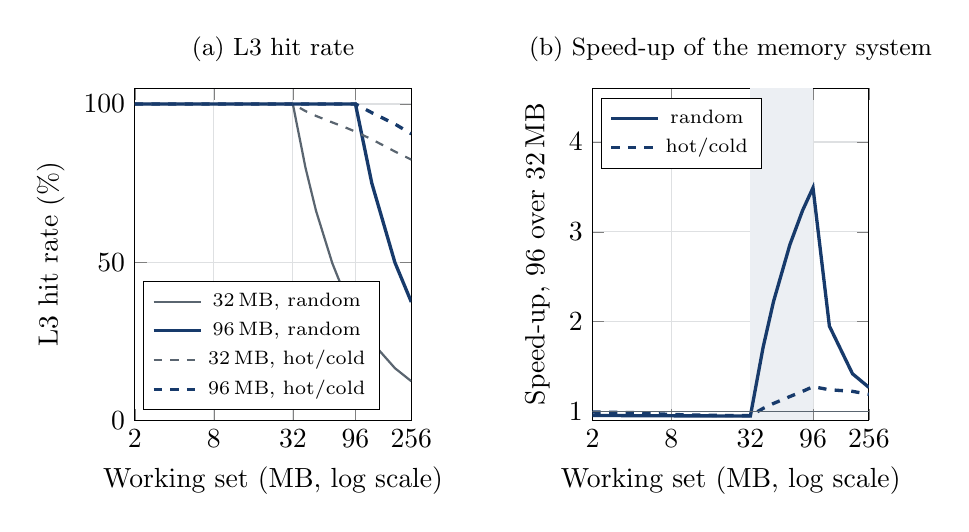
\begin{tikzpicture}
\begin{axis}[
  name=hit, width=0.42\textwidth, height=5.8cm,
  xmode=log, log basis x=2, xmin=2, xmax=256, ymin=0, ymax=105,
  xtick={2,8,32,96,256}, xticklabels={2,8,32,96,256},
  xlabel={Working set (MB, log scale)}, ylabel={L3 hit rate (\%)},
  title={\small (a) L3 hit rate}, legend style={font=\scriptsize,at={(0.03,0.03)},anchor=south west},
  grid=major, grid style={draftgray!20}]
\addplot[draftgray,thick] coordinates {(2,100) (4,100) (8,100) (16,100) (24,100) (32,100) (40,79.77) (48,66.33) (64,49.65) (80,39.63) (96,33) (128,24.74) (192,16.49) (256,12.36)};
\addlegendentry{32\,MB, random}
\addplot[draftblue,very thick] coordinates {(2,100) (4,100) (8,100) (16,100) (24,100) (32,100) (40,100) (48,100) (64,100) (80,100) (96,100) (128,74.94) (192,49.88) (256,37.41)};
\addlegendentry{96\,MB, random}
\addplot[draftgray,thick,dashed] coordinates {(2,100) (4,100) (8,100) (16,100) (24,100) (32,100) (40,97.74) (48,96.24) (64,94.18) (80,92.63) (96,91.26) (128,88.82) (192,84.98) (256,82.41)};
\addlegendentry{32\,MB, hot/cold}
\addplot[draftblue,very thick,dashed] coordinates {(2,100) (4,100) (8,100) (16,100) (24,100) (32,100) (40,100) (48,100) (64,100) (80,100) (96,100) (128,97.25) (192,93.66) (256,90.58)};
\addlegendentry{96\,MB, hot/cold}
\end{axis}
\begin{axis}[
  at={(hit.east)}, anchor=west, xshift=2.3cm, width=0.42\textwidth, height=5.8cm,
  xmode=log, log basis x=2, xmin=2, xmax=256, ymin=0.9, ymax=4.6,
  xtick={2,8,32,96,256}, xticklabels={2,8,32,96,256},
  xlabel={Working set (MB, log scale)}, ylabel={Speed-up, 96 over 32\,MB},
  title={\small (b) Speed-up of the memory system}, legend style={font=\scriptsize,at={(0.03,0.97)},anchor=north west},
  grid=major, grid style={draftgray!20}]
\fill[draftblue!8] (axis cs:32,0.9) rectangle (axis cs:96,4.6);
\addplot[draftblue,very thick] coordinates {(2,0.9557) (4,0.9519) (8,0.9502) (16,0.9494) (24,0.9491) (32,0.949) (40,1.714) (48,2.223) (64,2.857) (80,3.239) (96,3.491) (128,1.95) (192,1.419) (256,1.267)};
\addlegendentry{random}
\addplot[draftblue,very thick,dashed] coordinates {(2,0.9922) (4,0.987) (8,0.9653) (16,0.9558) (24,0.9532) (32,0.952) (40,1.033) (48,1.088) (64,1.165) (80,1.223) (96,1.275) (128,1.241) (192,1.223) (256,1.19)};
\addlegendentry{hot/cold}
\addplot[draftgray,thin] coordinates {(2,1) (256,1)};
\end{axis}
\end{tikzpicture}
\caption[S1: the effect of tripling the L3 against working-set size]{S1: the effect of tripling the L3 against the size of the working set, all else equal (one thread; overlap factor 0.335; mean of five seeds). (a) The L3 hit rate. (b) The model's memory-system time (exposed latency plus one cycle of other work per access) with 32\,MB divided by that with 96\,MB; values below 1 are the four extra cycles. The gain is confined to working sets between the two capacities (shaded) and fades beyond 96\,MB, the three regimes of \cref{fig:working-set}. Because almost every access in these synthetic workloads reaches the L3 or memory once the working set is well above the L2, the speed-ups are those of the memory system, not of a program.}
\label{fig:sim-working-set}
\end{figure}

\subsection{S2: Stacked, planar or beside?}
\label{sec:sim-designs}
No product offers a planar 96\,MB L3 or a cache die beside a Zen CCD, so here the model can only compare assumptions; its verdicts are only as good as the assumed latencies, which is why both are varied. \Cref{fig:sim-designs} sets five designs against the same random workload. The planar 96\,MB L3 is assumed to take 59 cycles, as the longer wires of \cref{sec:planar-limits} suggest. At that latency the stacked L3 has about 10\% lower exposed latency than the planar one at every working set up to 96\,MB (6.21 against 6.87\,ns at 32\,MB). For data that fits in 32\,MB both pay for their capacity: compared with the 32\,MB baseline (5.88\,ns), the planar design is 17\% slower and the stacked one 5.6\% slower.

\begin{figure}[htbp]
\centering
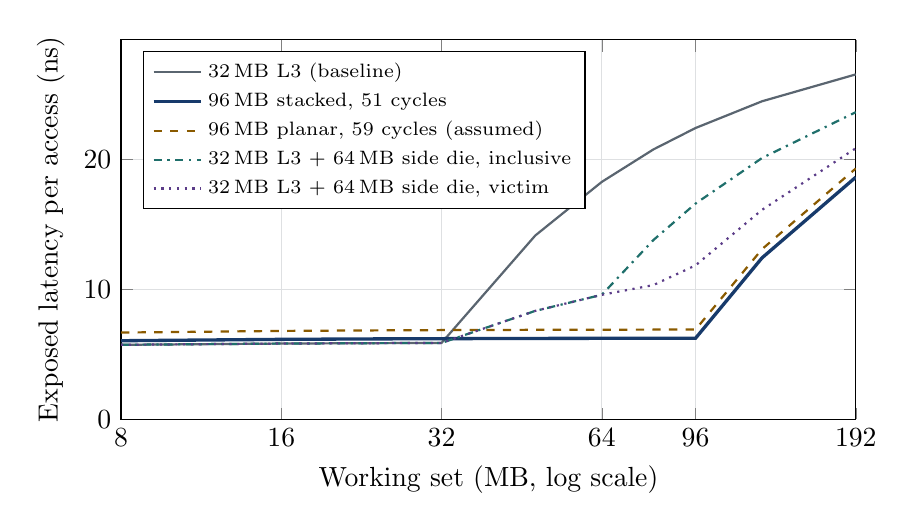
\begin{tikzpicture}
\begin{axis}[
  width=0.9\textwidth, height=6.4cm,
  xmode=log, log basis x=2, xmin=8, xmax=192, ymin=0,
  xtick={8,16,32,64,96,192}, xticklabels={8,16,32,64,96,192},
  xlabel={Working set (MB, log scale)}, ylabel={Exposed latency per access (ns)},
  legend pos=north west, legend style={font=\scriptsize}, legend cell align=left,
  grid=major, grid style={draftgray!20}]
\addplot[draftgray,thick] coordinates {(8,5.74) (16,5.836) (24,5.867) (32,5.884) (48,14.16) (64,18.29) (80,20.79) (96,22.44) (128,24.5) (192,26.57)};
\addlegendentry{32\,MB L3 (baseline)}
\addplot[draftblue,very thick] coordinates {(8,6.054) (16,6.16) (24,6.195) (32,6.213) (48,6.231) (64,6.24) (80,6.245) (96,6.248) (128,12.44) (192,18.65)};
\addlegendentry{96\,MB stacked, 51 cycles}
\addplot[mmamber,thick,dashed] coordinates {(8,6.683) (16,6.809) (24,6.851) (32,6.873) (48,6.894) (64,6.905) (80,6.911) (96,6.915) (128,13.11) (192,19.32)};
\addlegendentry{96\,MB planar, 59 cycles (assumed)}
\addplot[mmteal,thick,dash dot] coordinates {(8,5.74) (16,5.836) (24,5.867) (32,5.884) (48,8.354) (64,9.591) (80,13.81) (96,16.62) (128,20.13) (192,23.66)};
\addlegendentry{32\,MB L3 + 64\,MB side die, inclusive}
\addplot[mmpurple,thick,dotted] coordinates {(8,5.74) (16,5.836) (24,5.867) (32,5.884) (48,8.354) (64,9.591) (80,10.34) (96,11.86) (128,16.14) (192,20.88)};
\addlegendentry{32\,MB L3 + 64\,MB side die, victim}
\end{axis}
\end{tikzpicture}
\caption[S2: ways to provide about 96\,MB of last-level cache]{S2: ways to provide about 96\,MB of last-level cache, compared on the same random-access workload (one thread at 4\,GHz; average latency after the overlap factor of 0.335; mean of five seeds). The planar latency of 59 cycles is an assumption that \cref{tab:sim-planar} varies. The side die is a 64\,MB L4 at 22\,ns, either filled on every miss (inclusive) or filled by L3 evictions (victim); \cref{tab:sim-side-die} varies its latency.}
\label{fig:sim-designs}
\end{figure}

\Cref{tab:sim-planar} asks how slow a planar 96\,MB L3 could be and still beat the 32\,MB baseline. For working sets in the window, the answer is ``very slow'': 107 cycles at 40\,MB and 245 at 96\,MB, because almost any hit beats a trip to memory. In the model, latency is therefore not the planar design's main disadvantage for programs in that window. Its disadvantages lie elsewhere: programs whose working sets fit in 32\,MB pay every extra cycle and gain nothing, and the planar die costs area and yield, which the model cannot price (\cref{sec:manufacturing}). Stacking keeps the latency penalty small for programs that do not need the capacity, and it moves the area onto a die that only some products carry.

\begin{table}[htbp]
  \centering
  \caption[S2: the slowest planar 96\,MB L3 that still beats the baseline]{S2: the longest L3 latency at which a planar 96\,MB L3 still gives a shorter exposed latency than the 32\,MB, 47-cycle baseline (random accesses; overlap 0.335; found by bisection on the five-seed mean). The stacked design needs 51 cycles.}
  \label{tab:sim-planar}
  \small
  \begin{tabular}{@{}lcccccc@{}}
    \toprule
    \textbf{Working set (MB)} & 24 & 40 & 48 & 64 & 80 & 96 \\
    \midrule
    Break-even planar latency (cycles) & 47 & 107 & 147 & 196 & 226 & 245 \\
    \bottomrule
  \end{tabular}
\end{table}

The cache die beside the CCD is modelled as a 64\,MB L4 that is looked up after an L3 miss. Its default latency, 22\,ns, gives a hit of about 34\,ns in all, close to the more than 30\,ns that Lam measured for Broadwell's embedded DRAM (eDRAM); this is an assumption, and a modern 2.5D die could be faster. \Cref{tab:sim-side-die} therefore varies it from 5 to 22\,ns and compares two organisations. An \emph{inclusive} side die is filled on every miss and holds copies of L3 data, so the L3 and the side die together hold only 64\,MB of distinct data; a \emph{victim} side die is filled only by L3 evictions, so together they hold 96\,MB. The two are identical at 48\,MB, where both hold the data. At 80\,MB the victim die is much better (10.34 against 13.81\,ns at 22\,ns). For working sets beyond 32\,MB, however, the side die does not match the stacked L3 even at 5\,ns (6.46 against 6.23\,ns at 48\,MB), because in the model every side-die hit first pays a full L3 miss. Below 32\,MB the side die is the faster of the two (5.88 against 6.21\,ns at 32\,MB), because it adds nothing to an L3 hit, whereas the stacked L3 adds four cycles. Whether a real side die would be looked up after the L3 or alongside it is a design choice the model does not explore.

\begin{table}[htbp]
  \centering
  \caption[S2: a side die against the stacked L3]{S2: exposed latency per access (ns) of a 64\,MB side die beside a 32\,MB L3, by its own latency and organisation, against the stacked 96\,MB L3 (random accesses, one thread at 4\,GHz, overlap 0.335). An inclusive side die is filled on every miss and holds copies of L3 data; a victim side die is filled by L3 evictions. In the model the side die is looked up after an L3 miss.}
  \label{tab:sim-side-die}
  \small
  \begin{tabular}{@{}lcccc@{}}
    \toprule
    & \multicolumn{2}{c}{\textbf{48\,MB working set}} & \multicolumn{2}{c}{\textbf{80\,MB working set}} \\ \cmidrule(lr){2-3}\cmidrule(l){4-5}
    \textbf{Side-die latency} & \textbf{Inclusive} & \textbf{Victim} & \textbf{Inclusive} & \textbf{Victim} \\
    \midrule
    5\,ns & 6.46 & 6.46 & 11.53 & 6.93 \\
    8\,ns & 6.79 & 6.79 & 11.93 & 7.53 \\
    12\,ns & 7.24 & 7.24 & 12.47 & 8.33 \\
    16\,ns & 7.68 & 7.68 & 13.01 & 9.14 \\
    22\,ns & 8.35 & 8.35 & 13.81 & 10.34 \\
    Stacked 96\,MB L3 & 6.23 & 6.23 & 6.25 & 6.25 \\
    \bottomrule
  \end{tabular}
\end{table}

\subsection{S3: Cache against clock}
\label{sec:sim-clock}
To estimate an effect on time, S3 uses an access mix fitted to Lam's libx264 run (\cref{app:sim-setup}). Most accesses hit a 16\,KB hot region in the L1, a small share go to a cold region whose size is swept, and a smaller share go to a far region that misses in both caches, so that the V-Cache CCD keeps about 1.04 misses per thousand instructions, as Lam's V-Cache CCD kept about 1.08. Three inputs of the mix are assumptions, not measurements. They are one memory access per three instructions, the textbook's typical figure \cite[sec.~11.1.1]{sarangi2025basic}; one cycle for an L1 hit, standing for loads the pipeline hides; and 0.48 cycles of other work per access, chosen so that the plain CCD runs at about 730 cycles per thousand instructions, as libx264 did. The plain CCD runs at 5.15\,GHz and the V-Cache CCD at a lower clock, and the cold region grows from 32 to 96\,MB so that the larger cache removes more and more misses. \Cref{fig:sim-cache-clock} plots the result against the number of misses removed, and \cref{tab:sim-breakeven} reads off the break-even for each clock gap.

\begin{figure}[htbp]
\centering
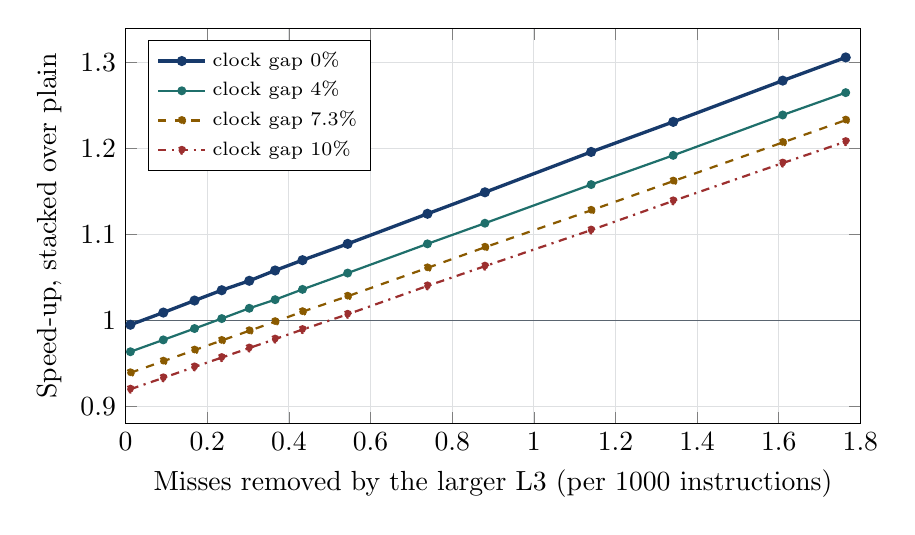
\begin{tikzpicture}
\begin{axis}[
  width=0.9\textwidth, height=6.6cm,
  xmin=0, xmax=1.8, ymin=0.88, ymax=1.34,
  xlabel={Misses removed by the larger L3 (per 1000 instructions)}, ylabel={Speed-up, stacked over plain},
  legend pos=north west, legend style={font=\scriptsize}, legend cell align=left,
  grid=major, grid style={draftgray!20}]
\addplot[draftgray,thin,forget plot] coordinates {(0,1) (1.8,1)};
\addplot[draftblue,very thick,mark=*,mark size=1.2pt] coordinates {(0.0117,0.9948) (0.0923,1.009) (0.1688,1.023) (0.2354,1.035) (0.3029,1.046) (0.3662,1.058) (0.4333,1.07) (0.5439,1.089) (0.7394,1.124) (0.8802,1.149) (1.1404,1.196) (1.3415,1.231) (1.6097,1.279) (1.7641,1.306)};
\addlegendentry{clock gap 0\%}
\addplot[mmteal,thick,mark=*,mark size=1.2pt] coordinates {(0.0117,0.9634) (0.0923,0.9772) (0.1688,0.9904) (0.2354,1.002) (0.3029,1.014) (0.3662,1.024) (0.4333,1.036) (0.5439,1.055) (0.7394,1.089) (0.8802,1.113) (1.1404,1.158) (1.3415,1.192) (1.6097,1.239) (1.7641,1.265)};
\addlegendentry{clock gap 4\%}
\addplot[mmamber,thick,dashed,mark=*,mark size=1.2pt] coordinates {(0.0117,0.9389) (0.0923,0.9524) (0.1688,0.9653) (0.2354,0.9765) (0.3029,0.9878) (0.3662,0.9984) (0.4333,1.01) (0.5439,1.028) (0.7394,1.061) (0.8802,1.085) (1.1404,1.128) (1.3415,1.162) (1.6097,1.207) (1.7641,1.233)};
\addlegendentry{clock gap 7.3\%}
\addplot[mmred,thick,dash dot,mark=*,mark size=1.2pt] coordinates {(0.0117,0.9198) (0.0923,0.933) (0.1688,0.9457) (0.2354,0.9566) (0.3029,0.9677) (0.3662,0.9781) (0.4333,0.9892) (0.5439,1.007) (0.7394,1.04) (0.8802,1.063) (1.1404,1.105) (1.3415,1.139) (1.6097,1.183) (1.7641,1.208)};
\addlegendentry{clock gap 10\%}
\end{axis}
\end{tikzpicture}
\caption[S3: cache against clock in the simulation]{S3: the V-Cache CCD (96\,MB, 51 cycles) at a lower clock against the plain CCD (32\,MB, 47 cycles) at 5.15\,GHz, as the working set grows and the larger cache removes more misses. The access mix is calibrated to Lam's libx264 run (about 3.8 L3 accesses per 1000 instructions, of which about 1.04 per 1000 instructions miss even in the larger cache); the overlap factor is 0.335. A 7.3\% gap is the 4.8 against 5.15\,GHz Lam measured on the 7950X3D. Each curve crosses 1 at the break-even of that clock gap; \cref{tab:sim-breakeven} compares the crossings with the analytical model of \cref{sec:cache-clock-model}.}
\label{fig:sim-cache-clock}
\end{figure}
\begin{table}[htbp]
  \centering
  \caption[S3: break-even misses removed for each clock gap]{S3: misses the larger L3 must remove per 1000 instructions for the V-Cache CCD to break even, read from \cref{fig:sim-cache-clock} by linear interpolation, against the analytical model of \cref{sec:cache-clock-model} at the same clocks (plain CCD at 5.15\,GHz; the analytical equal-clock value is 0.12 at 4.2\,GHz).}
  \label{tab:sim-breakeven}
  \small
  \begin{tabular}{@{}lcccccc@{}}
    \toprule
    \textbf{Clock gap} & 0\% & 2\% & 4\% & 6\% & 7.3\% & 10\% \\
    \midrule
    Simulation (overlap 0.335) & 0.04 & 0.13 & 0.22 & 0.32 & 0.38 & 0.50 \\
    Analytical model, \cref{eq:cache-clock-model} & 0.10 & 0.17 & 0.24 & 0.31 & 0.35 & 0.45 \\
    \bottomrule
  \end{tabular}
\end{table}

The simulation is consistent with the main result of \cref{sec:cache-clock-model}: the clock gap, not the extra latency, sets the break-even. Away from equal clocks the two agree closely, within 0.05 misses per thousand instructions at every gap from 2 to 10\%; at Lam's 7.3\% gap the V-Cache CCD needs 0.38 misses removed per thousand instructions in the simulation and 0.35 in the analytical model. This agreement is expected rather than independent, since both are built on the same calibration and the same structure. At equal clocks the two disagree, 0.04 against 0.10 when both use 5.15\,GHz (the analytical model gives 0.12 at the 4.2\,GHz of \cref{sec:cache-clock-model}). Most of the difference, a factor of about 2.4, comes from one assumption: the simulation's overlap factor hides two thirds of the four extra L3 cycles as well as of each memory access, while the analytical model charges all four cycles. Neither has been measured.

\Cref{tab:sim-s3-sensitivity} shows how far the break-even depends on the inputs. At equal clocks it hardly moves, 0.03 to 0.05. In the simulation the overlap factor scales both the saving of a removed miss and the cost of the four extra cycles, so it cancels, and only the memory latency moves the equal-clock break-even. At the realistic 7.3\% gap it is far more sensitive. With the overlap factors fitted to Cyberpunk~2077 and GHPC it rises to 0.58 and 1.05, and with no overlap it falls to 0.17, so across the overlap factors fitted to Lam's workloads, with the libx264 mix held fixed, it changes about threefold. The break-even at a realistic gap is therefore known only to within that range, and it depends most on how much of a miss a core hides.

\begin{table}[htbp]
  \centering
  \caption[Sensitivity of S3: the break-even when one input is changed]{Sensitivity of S3: the break-even (misses removed per 1000 instructions) when one input is changed. The overlap factors 0.202 and 0.105 are those that reproduce Lam's Cyberpunk~2077 and GHPC measurements (\cref{tab:sim-calibration}).}
  \label{tab:sim-s3-sensitivity}
  \small
  \begin{tabular}{@{}lcc@{}}
    \toprule
    \textbf{Changed input} & \textbf{Equal clocks} & \textbf{7.3\% clock gap} \\
    \midrule
    calibrated (overlap 0.335) & 0.04 & 0.38 \\
    overlap 0.202 (Cyberpunk) & 0.04 & 0.58 \\
    overlap 0.105 (GHPC) & 0.04 & 1.05 \\
    overlap 1.0 & 0.04 & 0.17 \\
    memory 60 ns & 0.05 & 0.46 \\
    memory 90 ns & 0.03 & 0.31 \\
    \bottomrule
  \end{tabular}
\end{table}

As a check on the mix, the simulation was run at equal clocks of 4.2\,GHz at the point where the V-Cache CCD removes 0.40 misses per thousand instructions, as Lam's libx264 run did. There the plain CCD makes 3.78 L3 accesses and 1.44 misses per thousand instructions and takes 729 cycles, and the V-Cache CCD gains 5.2\%, against 5.1\% from Lam's chart IPCs (Lam states 4.9\%). Because the mix and the overlap factor are both fitted to this one measurement, the agreement shows that the construction is consistent; it is not a test of the model.

\subsection{S4: The cost of the chiplet split}
\label{sec:sim-chiplet}
The model's default hop between dies is AMD's figure for one round trip between a CCD and the I/O die, under 9\,ns (\cref{sec:d2d}). In the two-die configuration it is charged on every transfer between the CCDs and on every memory access, which crosses to the I/O die. \Cref{fig:sim-pingpong} compares this with Reguly's core-to-core measurement (\cref{tab:core-to-core}). Only the ratio can be fitted; the absolute values can be compared only roughly. Reguly's test times one message, whereas the model's round trip contains two messages and two write upgrades, and the model's preset is a planar Zen~3 CCD at 4\,GHz rather than a Milan-X. With a 9\,ns hop, the model's ping-pong round trip between CCDs takes 2.2 times as long as within one CCD (108.5 against 49\,ns), against 4.5 times in the measurement (265 against 58.6\,ns). One transfer between two different CCDs, a request and its reply, crosses the CCD--IOD link four times, that is, two of AMD's round trips or 18\,ns; with an 18\,ns hop the model gives 2.9 times. Matching the measured ratio needs a hop of about 37\,ns. This value is fitted to a ratio; it is not the cost of a transfer. The model's exchanges are themselves too fast: halved as in \cref{sec:cross-ccd}, its round trips give about 25\,ns per message within a CCD against Reguly's 58.6\,ns, and about 110\,ns across CCDs with a 37\,ns hop against about 265\,ns, both about 2.4 times too fast. Matching Reguly's absolute extra cost would need a hop of about 97\,ns. The measured extra cost is the 206\,ns of \cref{sec:cross-ccd}, from one cloud instance, most of which lies in the fabric and the coherence steps rather than in the link itself. The group's 5600X gives the one check of the model's coherence timing on data it was not built from: the model's same-CCD round trip is 49\,ns at 4\,GHz, against 98.5\,ns measured under WSL2 (66--72\,ns on the fastest pairs; \cref{app:5600x}). The model's sharing latencies should therefore be read as lower estimates.

\begin{figure}[htbp]
\centering
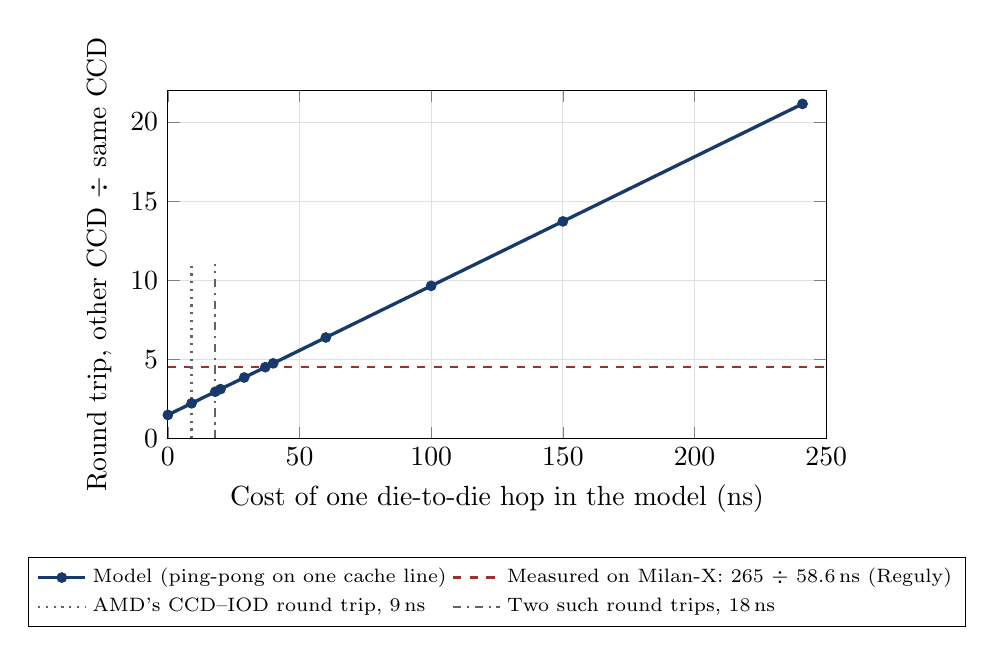
\begin{tikzpicture}
\begin{axis}[
  width=0.82\textwidth, height=6.0cm,
  xmin=0, xmax=250, ymin=0, ymax=22,
  xlabel={Cost of one die-to-die hop in the model (ns)}, ylabel={Round trip, other CCD $\div$ same CCD},
  legend columns=2, legend style={font=\scriptsize,at={(0.5,-0.34)},anchor=north}, legend cell align=left,
  grid=major, grid style={draftgray!20}]
\addplot[draftblue,very thick,mark=*,mark size=1.3pt] coordinates {(0,1.48) (9,2.214) (18,2.949) (20,3.112) (29,3.847) (37,4.5) (40,4.745) (60,6.378) (100,9.643) (150,13.72) (241,21.15)};
\addlegendentry{Model (ping-pong on one cache line)}
\addplot[mmred,thick,dashed] coordinates {(0,4.52) (250,4.52)};
\addlegendentry{Measured on Milan-X: 265 $\div$ 58.6\,ns (Reguly)}
\addplot[draftgray,thick,dotted] coordinates {(9,0) (9,11)};
\addlegendentry{AMD's CCD--IOD round trip, 9\,ns}
\addplot[draftgray,thick,dashdotted] coordinates {(18,0) (18,11)};
\addlegendentry{Two such round trips, 18\,ns}
\end{axis}
\end{tikzpicture}
\caption[S4: cross-CCD to same-CCD ping-pong ratio against hop cost]{S4: the model's ratio of cross-CCD to same-CCD ping-pong time as the cost of a hop grows (planar Zen~3 CCDs at 4\,GHz). Only the ratio is fitted to Reguly's measurement \cite{regulyComparativeEvaluationBandwidthbound2023}, because Reguly's test times one message while the model's round trip contains two messages and two write upgrades. One transfer between two different CCDs, a request and its reply, crosses the CCD--IOD link four times, two of AMD's 9\,ns round trips. With a 9\,ns hop the model gives 2.2$\times$ and with 18\,ns 2.9$\times$; matching the measured 4.5$\times$ needs a hop of about 37\,ns. That value is fitted to the ratio only: the model's exchanges are about 2.4 times faster than the measured ones, so 37\,ns is not the real cost of a transfer, which \cref{sec:cross-ccd} puts at about 206\,ns on one cloud instance.}
\label{fig:sim-pingpong}
\end{figure}

\Cref{tab:sim-split} then runs sixteen cores on two CCDs against a hypothetical single die with one 64\,MB L3 at the same 47 cycles, which favours the single die, since a real 64\,MB L3 would be slower (\cref{sec:planar-limits}). Two kinds of data are compared:
\begin{itemize}
  \item \textbf{Shared data}, a 48\,MB set read and written by all cores (5\% writes). It costs the two-die design in two ways. First, 66 of every thousand accesses cross between the CCDs. Second, each CCD keeps its own copy of the lines it reads, so the 48\,MB no longer fits in two 32\,MB L3s: the two-die design makes 22 memory accesses per thousand, the single die none. Its exposed latency is 1.20 times the single die's with a 9\,ns hop, 1.26 times with 18\,ns, the two link round trips a transfer between CCDs needs, and 1.39 times with the fitted 37\,ns. The 9\,ns figure undercounts the link and is therefore a lower limit. The 18 and 37\,ns figures also charge every memory access at that hop; with AMD's 9\,ns for memory accesses they would be about 1.25 and 1.35 times, by the authors' estimate. Because the 37\,ns hop matches only a ratio (\cref{fig:sim-pingpong}), 1.39 times is not an upper limit either.
  \item \textbf{Private data}, 8\,MB per thread, 128\,MB in all, which overflows both designs. Nothing crosses between the CCDs, but every memory access pays the hop to the I/O die, and the two-die design is 1.08 times slower with a 9\,ns hop. For memory accesses, AMD's 9\,ns is the relevant figure, not the 37\,ns fitted to sharing.
\end{itemize}
In the model, then, the split costs most for data shared across the boundary, where replication also wastes L3 capacity, and a few per cent for private data that misses to memory. This is the model's version of the argument for placing communicating threads on one CCD (\cref{sec:cross-ccd}). It follows from how the hop is charged, so it shows the size of the effect for the assumed costs rather than proving that the costs are right.

\begin{table}[htbp]
  \centering
  \caption[S4: two CCDs against a hypothetical single die]{S4: sixteen cores on two CCDs (2 $\times$ 32\,MB L3; the hop is charged on every transfer between CCDs and on every memory access) against a hypothetical single die with one 64\,MB L3 at the same 47 cycles, for four hop costs (overlap 0.335; mean of five seeds). The shared data set is 48\,MB, with 5\% of accesses writes; the private data sets are 8\,MB per thread, 128\,MB in all, and overflow both organisations.}
  \label{tab:sim-split}
  \footnotesize
  \begin{tabular}{@{}>{\raggedright\arraybackslash}p{1.4cm}c>{\centering\arraybackslash}p{2.3cm}>{\centering\arraybackslash}p{2.4cm}>{\centering\arraybackslash}p{2.1cm}>{\centering\arraybackslash}p{1.6cm}@{}}
    \toprule
    \textbf{Data} & \textbf{Hop (ns)} & \textbf{Transfers between CCDs per 1000 accesses} & \textbf{Memory accesses per 1000 (two dies / one die)} & \textbf{Exposed latency, two dies (ns)} & \textbf{Two dies $\div$ one die} \\
    \midrule
    shared & 9 & 66 & 22 / 0 & 6.83 & 1.20$\times$ \\
    shared & 18 & 66 & 22 / 0 & 7.17 & 1.26$\times$ \\
    shared & 37 & 66 & 22 / 0 & 7.90 & 1.39$\times$ \\
    shared & 60 & 66 & 22 / 0 & 8.77 & 1.54$\times$ \\
    private & 9 & 0 & 500 / 500 & 19.65 & 1.08$\times$ \\
    private & 18 & 0 & 500 / 500 & 21.15 & 1.17$\times$ \\
    private & 37 & 0 & 500 / 500 & 24.34 & 1.34$\times$ \\
    private & 60 & 0 & 500 / 500 & 28.19 & 1.55$\times$ \\
    \bottomrule
  \end{tabular}
\end{table}

\subsection{S5: Zen~2 to Zen~3, one factor at a time}
\label{sec:sim-zen2-zen3}
AMD's 19\% IPC gain from Zen~2 to Zen~3 combines a unified L3 with a redesigned core (\cref{sec:confounds}). The model can separate the two L3 changes: the unification and the 7--8 cycles it added (\cref{fig:sim-zen2-zen3}). For one thread with a working set of up to 16\,MB, the unified L3's exposed latency is about 12\% higher than that of the split Zen~2-style L3 (20\% higher in raw latency), entirely because the split L3 has the lower latency: with equal latencies the two organisations give identical results. Between 16 and 32\,MB the unified L3 is better by 1.7 to 3.0 times (exposed; 4.0 times in raw latency at 32\,MB), because a thread on a Zen~2 CCX can use only its own 16\,MB. With eight threads sharing one data set, the gain is smaller, 1.3 to 2.3 times, because a miss in one CCX's L3 can often be served from the other CCX's L3, at two L3 latencies plus the hop, instead of from memory. The unification is therefore worth a great deal for working sets between 16 and 32\,MB and costs 7--8 cycles on every L3 access elsewhere; for a real program that cost scales with how often it reaches the L3. Its contribution to an average over many programs depends entirely on how many of them fall in the window, which is why the 19\% figure cannot be credited to the L3.

\begin{figure}[htbp]
\centering
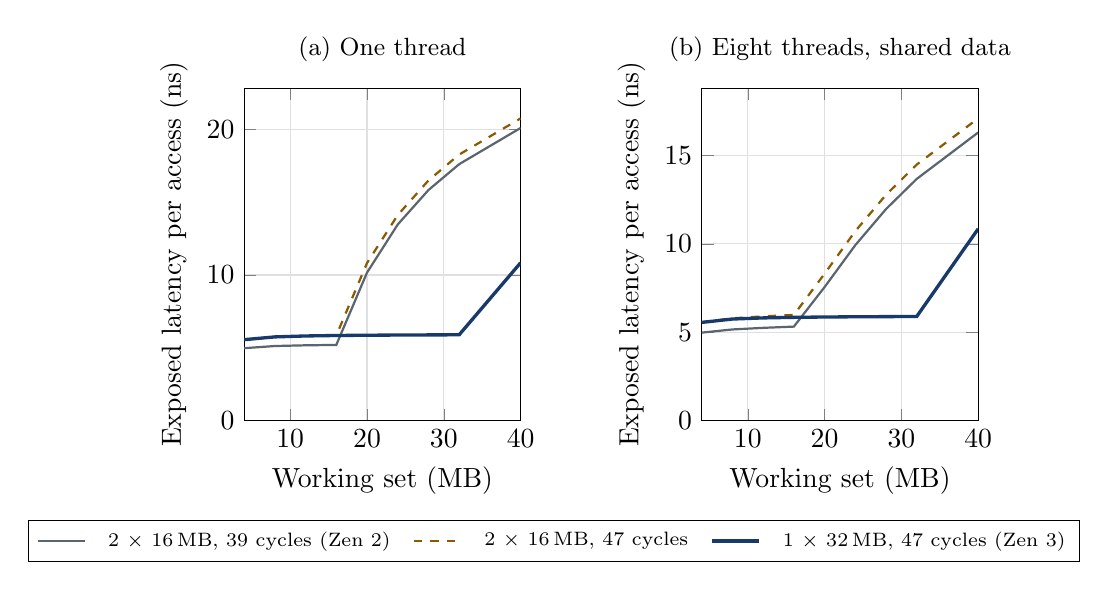
\begin{tikzpicture}
\begin{axis}[
  name=one,  width=0.42\textwidth, height=5.8cm, xmin=4, xmax=40, ymin=0,
  xlabel={Working set (MB)}, ylabel={Exposed latency per access (ns)}, title={\small (a) One thread}, legend columns=3, legend style={font=\scriptsize,at={(1.12,-0.30)},anchor=north,column sep=6pt}, legend cell align=left,
  grid=major, grid style={draftgray!20}]
\addplot[draftgray,thick] coordinates {(4,4.963) (8,5.112) (12,5.162) (16,5.187) (20,10.16) (24,13.47) (28,15.84) (32,17.62) (40,20.11)};
\addlegendentry{2 $\times$ 16\,MB, 39 cycles (Zen~2)}
\addplot[mmamber,thick,dashed] coordinates {(4,5.549) (8,5.74) (12,5.804) (16,5.836) (20,10.82) (24,14.12) (28,16.5) (32,18.28) (40,20.77)};
\addlegendentry{2 $\times$ 16\,MB, 47 cycles}
\addplot[draftblue,very thick] coordinates {(4,5.549) (8,5.74) (12,5.804) (16,5.836) (20,5.855) (24,5.867) (28,5.877) (32,5.884) (40,10.84)};
\addlegendentry{1 $\times$ 32\,MB, 47 cycles (Zen~3)}
\end{axis}
\begin{axis}[
  name=eight, at={(one.east)}, anchor=west, xshift=2.3cm, width=0.42\textwidth, height=5.8cm, xmin=4, xmax=40, ymin=0,
  xlabel={Working set (MB)}, ylabel={Exposed latency per access (ns)}, title={\small (b) Eight threads, shared data},
  grid=major, grid style={draftgray!20}]
\addplot[draftgray,thick,forget plot] coordinates {(4,4.97) (8,5.15) (12,5.241) (16,5.311) (20,7.551) (24,9.926) (28,11.97) (32,13.68) (40,16.31)};
\addplot[mmamber,thick,dashed,forget plot] coordinates {(4,5.557) (8,5.782) (12,5.892) (16,5.974) (20,8.308) (24,10.72) (28,12.78) (32,14.49) (40,17.11)};
\addplot[draftblue,very thick,forget plot] coordinates {(4,5.549) (8,5.74) (12,5.804) (16,5.836) (20,5.855) (24,5.868) (28,5.877) (32,5.884) (40,10.85)};
\end{axis}
\end{tikzpicture}
\caption[S5: Zen~2 to Zen~3 L3 organisation and latency, separated]{S5: the Zen~2 to Zen~3 change of L3 organisation, separated from the latency change (random accesses; average latency after the overlap factor of 0.335; mean of five seeds). Comparing the dashed line with the thick one isolates the unification itself, since both have a 47-cycle L3; comparing the thin solid line with the dashed one isolates the latency change.}
\label{fig:sim-zen2-zen3}
\end{figure}

\subsection{S6: When bandwidth binds}
\label{sec:sim-bandwidth}
\Cref{fig:sim-streaming} shows up to eight cores streaming through private data with two DDR4-3200 channels, 51.2\,GB/s. Here the overlap factor is set to 0.05, for a core whose prefetchers hide most latency. With 8\,MB per thread, the 32\,MB L3 holds the data of four threads; at five, the combined 40\,MB no longer fits, and throughput falls from 1.08 to 0.68 billion lines per second, limited by memory latency, before levelling off at the DRAM limit of 0.8 billion from six threads. The 96\,MB L3 holds all eight threads' data and keeps scaling to 2.1 billion, 2.7 times the DRAM limit. With 20\,MB per thread, the 96\,MB L3 holds the data of up to four threads; beyond that both caches overflow and meet the same limit. A larger L3 thus raises the bandwidth a chip can sustain only for data that fits in it. Beyond that, more cores add no throughput, which is the bandwidth wall of \cref{sec:bandwidth-wall}. The result follows directly from the model's time limits, so it illustrates the argument rather than testing it. The 5600X shows the same wall in practice (\cref{app:5600x}): six threads streaming from memory reach 41\,GB/s, 80\% of the 51.2\,GB/s peak and 6.8\,GB/s per core, while the same threads reading data that fits in the L3 (8--16\,MB in all) reach 280--296\,GB/s. The model's DRAM limit is the peak, so its absolute throughputs beyond the wall are about a quarter too high; the shape of the wall is the same.

\begin{figure}[htbp]
\centering
\begin{tikzpicture}
\begin{axis}[
  width=0.82\textwidth, height=6.2cm, xmin=1, xmax=8, ymin=0, ymax=2.3,
  xlabel={Threads, each streaming through its own data}, ylabel={Lines delivered (10$^9$ per second)},
  legend pos=north west, legend style={font=\scriptsize}, legend cell align=left,
  grid=major, grid style={draftgray!20}]
\addplot[mmred,thin,dashed,forget plot] coordinates {(1,0.8) (8,0.8)};
\node[font=\scriptsize,mmred,anchor=south east] at (axis cs:8,0.8) {DRAM limit: 51.2\,GB/s $\div$ 64\,B};
\addplot[draftgray,thick,mark=*,mark size=1.2pt] coordinates {(1,0.2712) (2,0.5424) (3,0.8136) (4,1.085) (5,0.6768) (6,0.8) (7,0.8) (8,0.8)};
\addlegendentry{32\,MB L3, 8\,MB per thread}
\addplot[draftblue,very thick,mark=*,mark size=1.2pt] coordinates {(1,0.2676) (2,0.5351) (3,0.8027) (4,1.07) (5,1.338) (6,1.605) (7,1.873) (8,2.14)};
\addlegendentry{96\,MB L3, 8\,MB per thread}
\addplot[draftgray,thick,dashed,mark=*,mark size=1.2pt] coordinates {(1,0.2712) (2,0.2707) (3,0.4061) (4,0.5415) (5,0.6768) (6,0.8) (7,0.8) (8,0.8)};
\addlegendentry{32\,MB L3, 20\,MB per thread}
\addplot[draftblue,very thick,dashed,mark=*,mark size=1.2pt] coordinates {(1,0.2676) (2,0.5351) (3,0.8027) (4,1.07) (5,0.7731) (6,0.8) (7,0.8) (8,0.8)};
\addlegendentry{96\,MB L3, 20\,MB per thread}
\end{axis}
\end{tikzpicture}
\caption[S6: up to eight cores streaming through private data]{S6: up to eight cores streaming through private data (sequential reads; overlap 0.05, for a core whose prefetchers hide most latency; 51.2\,GB/s of DRAM bandwidth; mean of five seeds). While the combined data fits in the L3, throughput grows with the number of threads; once it does not, every configuration meets the same DRAM limit. With 8\,MB per thread, the 96\,MB L3 holds all eight threads' data and keeps scaling to 2.1 billion lines per second, while the 32\,MB L3 overflows at five threads and falls back to the DRAM limit.}
\label{fig:sim-streaming}
\end{figure}

\subsection{Sensitivity to the assumed inputs}
\label{sec:sim-sensitivity}
\Cref{tab:sim-sensitivity} repeats the S1 comparison with one input changed at a time, and \cref{tab:sim-s3-sensitivity} did the same for S3. In S1 the pattern holds in every case: a loss (one minus the speed-up) of 2.4--9.6\% when the data fits in 32\,MB, a gain of 1.89 to 3.78 times at 64\,MB, and a smaller gain beyond 96\,MB. The size of the gain in the window depends on the overlap factor and on memory latency, from 34\% below to 32\% above the calibrated 2.86 times, so the model fixes the direction and the window but not the size of the effect. \Cref{tab:sim-policy} varies the replacement policy. With random accesses no policy can change the result, since every resident line is equally likely to be used next, and the three policies agree to within 0.05\%. With reuse or a cyclic order the policy matters: for hot/cold accesses the gain at 64\,MB ranges from 1.15 to 1.19 times, and for cyclic sequential accesses from 4.27 to 4.75 times. In every case the larger cache still wins in the window and loses slightly when the data fits. A stacked L3 at 55 rather than 51 cycles almost doubles the loss when the data fits, from 5.1 to 9.6\%, which shows why AMD's four-cycle figure matters (\cref{sec:vcache-access}).

\begin{table}[htbp]
  \centering
  \caption[Sensitivity of S1 to the assumed inputs]{Sensitivity of S1: the memory-system speed-up of 96 over 32\,MB (as in \cref{fig:sim-working-set}b, random accesses) when one assumed input is changed at a time. A 16\,MB working set fits in both caches, 64\,MB lies between them and 192\,MB exceeds both.}
  \label{tab:sim-sensitivity}
  \small
  \begin{tabular}{@{}lccc@{}}
    \toprule
    \textbf{Changed input} & \textbf{16\,MB} & \textbf{64\,MB} & \textbf{192\,MB} \\
    \midrule
    none (calibrated defaults) & 0.95 & 2.86 & 1.42 \\
    overlap 0.105 (GHPC) & 0.98 & 1.89 & 1.30 \\
    overlap 0.202 (Cyberpunk) & 0.96 & 2.40 & 1.38 \\
    overlap 1.0 & 0.92 & 3.78 & 1.47 \\
    memory 60 ns & 0.95 & 2.50 & 1.38 \\
    memory 90 ns & 0.95 & 3.27 & 1.45 \\
    stacked L3 55 cycles & 0.90 & 2.72 & 1.39 \\
    \bottomrule
  \end{tabular}
\end{table}
\begin{table}[htbp]
  \centering
  \caption[Replacement policy and the gain from a larger L3]{Replacement policy: the memory-system speed-up of 96 over 32\,MB for three workloads under three policies (overlap 0.335; mean of five seeds). With random accesses every resident line is equally likely to be used next, so no policy can change the result; the policy matters for workloads with reuse or a cyclic order.}
  \label{tab:sim-policy}
  \small
  \begin{tabular}{@{}llccc@{}}
    \toprule
    \textbf{Workload} & \textbf{Policy} & \textbf{16\,MB} & \textbf{64\,MB} & \textbf{192\,MB} \\
    \midrule
    random & LRU & 0.95 & 2.86 & 1.42 \\
     & random & 0.95 & 2.86 & 1.42 \\
     & tree pseudo-LRU & 0.95 & 2.86 & 1.42 \\
    hot/cold & LRU & 0.96 & 1.16 & 1.22 \\
     & random & 0.96 & 1.19 & 1.22 \\
     & tree pseudo-LRU & 0.96 & 1.15 & 1.16 \\
    sequential (cyclic) & LRU & 0.95 & 4.75 & 0.99 \\
     & random & 0.95 & 4.27 & 0.99 \\
     & tree pseudo-LRU & 0.95 & 4.75 & 0.99 \\
    \bottomrule
  \end{tabular}
\end{table}

\subsection{What the model adds, and what it cannot show}
\label{sec:sim-limits}
With every other factor held fixed, the model reproduces, largely by construction, the patterns that the published evidence reached only through comparisons that change several things at once. The benefit of a larger L3 is confined to a window of working-set sizes (S1). The extra latency of the stacked cache is a small but real cost outside that window (S1, S2, sensitivity). The clock gap sets the break-even more than the extra latency does (S3). And the split costs most for data shared across dies (S4). Its value lies less in these reproductions than in the questions it lets the paper ask under stated assumptions. Within the model:
\begin{itemize}
  \item a planar 96\,MB L3 loses mainly on programs that do not need the capacity (S2);
  \item for working sets beyond 32\,MB, a side die looked up after the L3 cannot match a stacked L3 even at 5\,ns, and only a victim organisation makes full use of its capacity; below 32\,MB the side die is the faster (S2);
  \item the break-even at a realistic clock gap varies about threefold across the overlap factors of Lam's workloads (S3);
  \item the two link round trips of one transfer between CCDs, 18\,ns, explain only part of the measured cost of sharing between them (S4);
  \item the Zen~3 L3 unification helps only a window of working sets, so it cannot account for an average IPC gain on its own (S5).
\end{itemize}

The model has clear limits, which bound how its results may be used:
\begin{itemize}
  \item It has no pipeline, prefetchers, TLB or clock behaviour, so it gives the time spent in the memory system, not IPC or frame rates. The S3 mix is fitted to one program and contains three assumed inputs.
  \item Its workloads are synthetic. Traces of real programs through Valgrind were tried but were too slow to finish (several hundred times slowdown), so none is reported.
  \item It maps each working set contiguously and accesses it at random, so it has no conflict misses below capacity and keeps some hits that a cyclic access pattern would lose. It is therefore optimistic near each capacity edge, as the 5600X measurement shows; for a latency sweep it understates the gain from about 20 to 64\,MB and overstates it close to 96\,MB (S0).
  \item Its L3 is filled on every miss; the sources used here do not state how Zen's L3 is filled, and real fill policies may differ. Its link-bandwidth limit is switched off in every experiment.
  \item Its key inputs are fitted or assumed: the overlap factor is fitted to measurements and the 37\,ns hop to a measured ratio, and the latencies of the planar 96\,MB L3 and of the side die are assumptions. Each is varied above where it matters.
  \item Its energy model has placeholder values and is not used in this paper.
\end{itemize}
Within these limits, the model's role is the one set out at the start of this section: a controlled illustration of the published evidence, not a substitute for it. What the 5600X measurements add is set out in S0 (\cref{sec:sim-calibration}).

\section{Summary of Part V}
In answer to RQ4, the stacked L3 costs about four cycles of L3 latency in every generation measured, and in its first two generations also several percent of clock speed. In exchange it removes capacity misses for working sets between 32 and 96\,MB per CCD. Where those misses dominate, the benefit is large: from about 10--20\% higher IPC in miss-heavy games (a geometric mean of 11.4\% over Lam's five quantified workloads at equal clock, \cref{sec:lam-detail}) to more than 1.5$\times$ in memory-bound computational fluid dynamics (OpenFOAM), and up to 3.4$\times$ for one HPC proxy at favourable problem sizes. Where they do not, the benefit is small, absent or slightly negative. The fourth generation repeats the pattern: Genoa-X gains up to 1.60$\times$ in OpenFOAM over a wider range of problem sizes, with almost no loss on small ones (\cref{sec:genoax}). The apparent value of each removed miss also varies, from about 50 to about 130 cycles in Lam's data, possibly because workloads with many misses overlap them, or because the counters include prefetches (\cref{tab:lam-per-miss}). Separating the cache effect from other factors requires fixed-clock comparisons or performance counters, which most vendor comparisons lack. The simulation of \cref{sec:sim-study} illustrates these patterns with every other factor held fixed, largely by construction: the working-set window, the small cost of the extra latency and the dominance of the clock gap at the break-even. It adds that the break-even at a realistic clock gap changes about threefold across the overlap factors fitted to Lam's workloads, and that the chiplet split costs most for data shared between dies. On the group's Ryzen~5 5600X the model's input latencies are nearly right, but close to each cache's capacity its latency is too low (\cref{sec:sim-calibration}). The confidence of these conclusions is therefore high for the direction of the effect and for its latency cost, moderate for the size of the IPC gain, which rests on one controlled study, and lower still for the size of the effect in any particular workload.
\clearpage
\part{Comparative Synthesis, Limitations and Future Directions}
\label{part:synthesis}
\Cref{fig:mindmap-synthesis} maps the topics of this part.

\mapfigure{%
\node[mmroot] (r) {Synthesis};
\node[mmbox,mmlevel1,fill=mmCFE0F4] (b0) at (0.00,3.60) {Three designs compared};
\draw[mmbig] (r) -- (b0);
\node[mmlevel2,mmbox,fill=mmF9D7AF] (b0c0) at (-3.05,5.35) {Monolithic};
\draw[mmsmall] (b0.north) to[out=90,in=-90] (b0c0.south);
\node[mmlevel2,mmbox,fill=mmF9D7AF] (b0c1) at (0.00,5.35) {Chiplets};
\draw[mmsmall] (b0.north) to[out=90,in=-90] (b0c1.south);
\node[mmlevel2,mmbox,fill=mmF9D7AF] (b0c2) at (3.05,5.35) {Chiplets with stacked cache};
\draw[mmsmall] (b0.north) to[out=90,in=-90] (b0c2.south);
\node[mmbox,mmlevel1,fill=mmCFE7E1] (b1) at (4.07,2.20) {Other ways to a big LLC};
\draw[mmbig] (r) -- (b1);
\node[mmlevel2,mmbox,fill=mmF9D7AF] (b1c0) at (7.67,3.65) {eDRAM L4};
\draw[mmsmall] (b1.east) to[out=0,in=180] (b1c0.west);
\node[mmlevel2,mmbox,fill=mmF9D7AF] (b1c1) at (7.67,2.20) {Stacked DRAM, STT-RAM};
\draw[mmsmall] (b1.east) to[out=0,in=180] (b1c1.west);
\node[mmlevel2,mmbox,fill=mmF9D7AF] (b1c2) at (7.67,0.75) {HBM for bandwidth};
\draw[mmsmall] (b1.east) to[out=0,in=180] (b1c2.west);
\node[mmbox,mmlevel1,fill=mmF9D7AF] (b2) at (4.07,-2.20) {Interactions};
\draw[mmbig] (r) -- (b2);
\node[mmlevel2,mmbox,fill=mmDCCFF6] (b2c0) at (7.67,-0.75) {Small CCD makes stacking practical};
\draw[mmsmall] (b2.east) to[out=0,in=180] (b2c0.west);
\node[mmlevel2,mmbox,fill=mmDCCFF6] (b2c1) at (7.67,-2.20) {L3 private to each CCD};
\draw[mmsmall] (b2.east) to[out=0,in=180] (b2c1.west);
\node[mmlevel2,mmbox,fill=mmDCCFF6] (b2c2) at (7.67,-3.65) {Mixed CCDs need scheduling};
\draw[mmsmall] (b2.east) to[out=0,in=180] (b2c2.west);
\node[mmbox,mmlevel1,fill=mmF4AAA2] (b3) at (0.00,-3.60) {Remaining bottlenecks};
\draw[mmbig] (r) -- (b3);
\node[mmlevel2,mmbox,fill=mmCFE7E1] (b3c0) at (-3.05,-5.35) {Die-to-die hop};
\draw[mmsmall] (b3.south) to[out=-90,in=90] (b3c0.north);
\node[mmlevel2,mmbox,fill=mmCFE7E1] (b3c1) at (0.00,-5.35) {Bandwidth per core};
\draw[mmsmall] (b3.south) to[out=-90,in=90] (b3c1.north);
\node[mmlevel2,mmbox,fill=mmCFE7E1] (b3c2) at (3.05,-5.35) {Heat from stacks};
\draw[mmsmall] (b3.south) to[out=-90,in=90] (b3c2.north);
\node[mmoval,mmlevel1,fill=mmDCCFF6] (b4) at (-4.07,-2.20) {Evidence check};
\draw[mmbig] (r) -- (b4);
\node[mmlevel2,mmbox,fill=mmF4C2BB] (b4c0) at (-7.67,-0.75) {Strength of each claim};
\draw[mmsmall] (b4.west) to[out=180,in=0] (b4c0.east);
\node[mmlevel2,mmbox,fill=mmF4C2BB] (b4c1) at (-7.67,-2.20) {The case against};
\draw[mmsmall] (b4.west) to[out=180,in=0] (b4c1.east);
\node[mmlevel2,mmbox,fill=mmF4C2BB] (b4c2) at (-7.67,-3.65) {Threats to validity};
\draw[mmsmall] (b4.west) to[out=180,in=0] (b4c2.east);
\node[mmbox,mmlevel1,fill=mmD6EBC6] (b5) at (-4.07,2.20) {Outlook};
\draw[mmbig] (r) -- (b5);
\node[mmlevel2,mmoval,fill=mmDCCFF6] (b5c0) at (-7.67,3.65) {Future integration};
\draw[mmsmall] (b5.west) to[out=180,in=0] (b5c0.east);
\node[mmlevel2,mmbox,fill=mmDCCFF6] (b5c1) at (-7.67,2.20) {Implications for practice};
\draw[mmsmall] (b5.west) to[out=180,in=0] (b5c1.east);
\node[mmlevel2,mmoval,fill=mmDCCFF6] (b5c2) at (-7.67,0.75) {Open questions};
\draw[mmsmall] (b5.west) to[out=180,in=0] (b5c2.east);
}{[Overview of Part~\ref{part:synthesis}]{Overview of Part~\ref{part:synthesis}. The three bottlenecks at the bottom are the ones that remain after both techniques are applied (\cref{sec:remaining-bottlenecks}); the evidence-check branch is where each conclusion is graded.}}{fig:mindmap-synthesis}

\section{Monolithic, Chiplet-Based and Vertically Stacked Designs Compared}
\label{sec:comparison}

\Cref{tab:three-way} compares the three organisations against the bottleneck--benefit--trade-off test of \cref{sec:rq}, with the measured or modelled values from Parts~\ref{part:chiplets}--\ref{part:case-study} where they exist.

\begin{table}[htbp]
  \centering
  \caption[Comparison of the three design approaches]{Comparison of the three design approaches (model values illustrative; measured values from the cited sections).}
  \label{tab:three-way}
  \small
  \begin{tabularx}{\textwidth}{@{}>{\raggedright\arraybackslash}p{2.6cm}>{\raggedright\arraybackslash}X>{\raggedright\arraybackslash}X>{\raggedright\arraybackslash}X@{}}
    \toprule
    & \textbf{Monolithic die} & \textbf{Chiplets (2D package)} & \textbf{Chiplets with stacked cache} \\
    \midrule
    Main limit addressed & --- & Die size, yield, uneven node scaling & Planar cost and wire length of a large LLC \\
    Communication & All on-die & Die-to-die links through the package & Adds dense vertical links between cache and compute dies \\
    Memory latency & Shortest on-die paths (no advantage visible in the Cezanne comparison, \cref{sec:cezanne}) & Extra die-to-die hop to memory & Fewer trips to memory for cache-sensitive work \\
    Cost and yield & Falls steeply with die area & Smaller dies, mixed nodes, tested before assembly & Extra die and bonding step; capacity only where sold \\
    Thermal & One heat source per die & Heat spread over several dies & Stack alters heat path from cores \\
    New trade-off & Scaling ceiling & Latency, link power, packaging & Heat, test complexity, workload dependence \\
    \midrule
    64-core compute sets per wafer (model) & about 35 & about 95 & about 95, plus cache dies \\
    L3 per compute die (Zen~3) & --- & 32\,MB & 96\,MB \\
    L3 hit latency (Milan / Milan-X) & --- & 47.5 cycles & 51.1 cycles \\
    Clock (Zen~4 desktop, same package) & --- & reference & about 7\% lower \\
    \bottomrule
  \end{tabularx}
\end{table}

\section{Other Ways to Enlarge the Last-Level Cache}
\label{sec:llc-alternatives}
3D V-Cache is one of several ways to give a processor more last-level cache. \Cref{tab:llc-alternatives} places it beside the alternatives for which the sources give numbers.

\begin{table}[htbp]
  \centering
  \caption[Ways to enlarge the last-level cache]{Ways to enlarge the last-level cache, and one way to raise memory bandwidth instead, with the figures the sources report (different studies, nodes and conditions; compare orders of magnitude, not exact values).}
  \label{tab:llc-alternatives}
  \small
  \begin{tabularx}{\textwidth}{@{}>{\raggedright\arraybackslash}p{2.6cm}>{\raggedright\arraybackslash}X>{\raggedright\arraybackslash}X>{\raggedright\arraybackslash}p{1.5cm}@{}}
    \toprule
    \textbf{Approach} & \textbf{Reported figures} & \textbf{Main drawback} & \textbf{Source} \\
    \midrule
    Planar SRAM L3 & 32\,MB per Zen~3 CCD; about 47 cycles & Die area, yield and wire length grow with capacity & \cite{cozmaAMDsVCacheTested2022,7-cpu.comAMDZen3} \\
    Stacked SRAM (3D V-Cache) & 64\,MB in 41\,mm$^2$; $+4$ cycles; $>$2\,TB/s (AMD peak) & Heat path, clocks, bonding cost & \cite{wuu2022vcache,cozmaDeepDivingZen2022} \\
    On-package eDRAM L4 (Intel Broadwell, side by side) & 128\,MB; over 30\,ns; about 50\,GB/s & Too slow to join the L3; must be a separate L4 & \cite{lamAMDs7950X3DZen2023} \\
    Stacked DRAM cache (simulated, 2006) & 32\,MB; average 13\% fewer cycles per memory access; off-die traffic $-66\%$; $+0.08$\,\textdegree C & Higher latency than SRAM; large tag store & \cite{blackStacking3DMicroarchitecture2006,mittalSurveyTechniquesArchitecting2016} \\
    On-package HBM as main memory (Intel Xeon Max 9480) & STREAM 1446\,GB/s against 310\,GB/s for two-socket Milan-X; cache-to-memory bandwidth ratio 3.8$\times$ against 14$\times$ & Raises bandwidth, not cache capacity; communication latency unchanged & \cite{regulyComparativeEvaluationBandwidthbound2023} \\
    STT-RAM (simulated, 16\,MB) & 5.0 against 11.4\,mm$^2$ for SRAM; leakage 65 against 463\,mW; write 11.9 against 3.3\,ns & Slow, energy-hungry writes & \cite{kimExploitingDataCompression2022} \\
    \bottomrule
  \end{tabularx}
\end{table}

\textbf{A side-by-side cache in practice.} Intel's Broadwell processors offer a real example of the side-by-side cache die discussed in \cref{sec:horizontal-vs-vertical}. They placed a 128\,MB embedded-DRAM die next to the processor die and used it as a fourth-level cache. Lam measured its latency at over 30\,ns (34.18\,ns in Lam's chart, against 10.63\,ns for the 7950X3D's V-Cache CCD) and its bandwidth at about 50\,GB/s, a quarter of Broadwell's own L3 bandwidth. Lam explains why: reaching the eDRAM involves another trip over the on-chip ring bus and then Intel's on-package I/O (OPIO) link, which on the related Haswell design is a 64-bit full-duplex interface at 6.4\,GT/s, providing 51.2\,GB/s in each direction \cite{lamAMDs7950X3DZen2023}. Because the eDRAM was too slow to be part of the L3, the L3 stayed in place to protect the cores from its latency, and Broadwell even used part of the L3's data array to hold the tags for the L4 \cite{lamAMDs7950X3DZen2023}. Lam contrasts this with V-Cache: each nominally 4\,MB slice of the Zen~4 L3 gets its own interface to an 8\,MB extension on the cache die, complete with tag and LRU arrays, so the stacked SRAM can extend the L3 rather than add a level \cite{lamAMDs7950X3DZen2023}. Lam also notes that Zen~4's own Infinity Fabric link between dies provides only about 64\,GB/s of read bandwidth per CCD, little better than Broadwell's link, and concludes that package traces are not well suited to L3 bandwidths \cite{lamAMDs7950X3DZen2023}. This is the comparison of \cref{tab:horizontal-vs-vertical} with real numbers: the side-by-side cache had about three times the latency of the stacked one and, in Lam's multithreaded test, about a thirteenth of its bandwidth (53 against 702\,GB/s), and it had to sit at a different level of the hierarchy \cite{lamAMDs7950X3DZen2023}. The 702\,GB/s is consistent with the 4.8\,GHz the V-Cache CCD sustained at stock clocks (\cref{sec:vcache-access}).

\textbf{Denser memory technologies.} The two simulated alternatives trade speed for density in different ways. Kim \emph{et al.}'s circuit-level estimates for 16\,MB caches show STT-RAM needing less than half the area of SRAM (5.0 against 11.4\,mm$^2$) and about a seventh of the leakage power (65 against 463\,mW). STT-RAM has a similar read latency (6.9 against 6.6\,ns) but a write latency more than three times longer (11.9 against 3.3\,ns) and about six times the write energy (1.13 against 0.18\,nJ) \cite[Table~1]{kimExploitingDataCompression2022}. That is why they place write-intensive blocks in a small SRAM region, an approach that gave a 26\% average speedup over a baseline placement policy in their simulations \cite{kimExploitingDataCompression2022}. Black \emph{et al.}'s 32\,MB stacked DRAM cache reduced the cycles per memory access of their benchmarks by 13\% on average and up to 55\%, cut off-die bandwidth and bus power by 66\%, and raised the peak temperature by only 0.08\,\textdegree C, much less than stacked SRAM, because DRAM dissipates less power \cite{blackStacking3DMicroarchitecture2006}. Neither has appeared in a mainstream CPU as an L3 extension; V-Cache's advantage is that it changes the cache's location but not its technology, so it adds capacity at nearly SRAM speed.

\section{Interactions Between Chiplet Organisation and Cache Design}
\label{sec:interactions}
The two techniques studied in this paper work as layers of one design, and they interact in four ways.

\textbf{The chiplet makes the stack practical.} Stacking is applied to a small, self-contained compute die. Because the CCD is small, a defective stack loses only one CCD's worth of silicon. Because the same CCD is used across the product line, AMD could design V-Cache support into it ``from Day~1'' and then offer stacked and unstacked versions of the same die \cite[slide~10]{wuu2022vcache}. And because the V-Cache CCD is built to the same height as a plain one, server parts with and without V-Cache share a package \cite[slide~17]{wuu2022vcache}.

\textbf{Stacking moves the cost of the cache to where it is wanted.} On a planar die every CCD would pay for a 96\,MB L3 whether or not its workload needs it, which is the ``product flexibility'' barrier on AMD's own list \cite[slide~6]{wuu2022vcache}. With stacking, the base CCD stays at 81\,mm$^2$ and the 41\,mm$^2$ cache die is added only to the products that benefit.

\textbf{The chiplet boundary also bounds the cache.} The L3 remains private to each CCD (\cref{sec:multicore}), so a thread gains only from the stacked cache on its own die, and data shared across CCDs still crosses the die-to-die link. A larger per-CCD L3 reduces trips to memory through the IOD, which partly offsets the chiplet's main latency cost (\cref{sec:d2d}), but it does nothing for traffic between CCDs.

\textbf{Mixing stacked and plain CCDs creates a scheduling problem.} Because stacking is per CCD, a product can combine a V-Cache CCD with a plain one, as the 16-core Ryzen~9 7950X3D does. The two CCDs then have different strengths: one has three times the L3, the other clocks about 7\% higher, and neither is better for every program. At the time of Lam's testing, AMD's default policy placed ordinary applications on the higher-clocked CCD, so a user had to set processor affinity by hand to use the cache \cite{lamAMDs7950X3DZen2023}. The chiplet organisation thus turns a hardware choice into an operating-system decision about where each thread should run.

\section{Workload-Dependent Trade-Offs and Remaining Bottlenecks}
\label{sec:remaining-bottlenecks}
Parts~III--V suggest a simple map of where each technique helps. Throughput workloads with many independent threads favour more cores, which chiplets supply. Workloads whose working sets lie just beyond a CCD's planar L3 favour stacked cache. Latency-sensitive single-threaded code with a small working set favours clock frequency, which a V-Cache part may sacrifice (\cref{sec:confounds}).

\Cref{fig:stacking-decision} turns this map into a sequence of questions for the stacked cache.

\begin{figure}[htbp]
\centering
\begin{tikzpicture}[x=1cm,y=1cm,
  q/.style={draw=draftblue,fill=draftlight,rounded corners=3pt,font=\scriptsize,align=center,text width=3.9cm,minimum height=1.0cm},
  a/.style={draw=draftgray,fill=white,font=\scriptsize,align=center,text width=3.6cm,minimum height=0.9cm},
  win/.style={a,draw=todored,fill=todored!8},
  arr/.style={-{Stealth[length=2mm]},draftblue,thick},
  lab/.style={font=\scriptsize\itshape,text=draftgray}]
\node[q] (q1) at (0,0) {Does the program miss often in the plain L3?\\(L3 misses per 1000 instructions)};
\node[a] (a1) at (5.6,0) {Few misses: prefer the higher-clocked plain CCD\\(flight simulator, 0.35 MPKI)};
\node[q] (q2) at (0,-2.0) {Does its working set fit in about three times the base L3?};
\node[a] (a2) at (5.6,-2.0) {Far larger, or streaming: little change; needs memory bandwidth\\(largest MiniFE inputs)};
\node[q] (q3) at (0,-4.0) {Is the IPC gain at equal clock larger than the plain CCD's clock advantage (about 5--7\%)?};
\node[a] (a3) at (5.6,-4.0) {Roughly a tie or a small loss\\(libx264: $+4.9\%$ IPC against $+7\%$ clock)};
\node[win] (a4) at (0,-6.0) {Stacked cache wins\\(Call of Duty, Cyberpunk~2077, mid-sized OpenFOAM and MiniFE)};
\draw[arr] (q1) -- node[lab,above]{no} (a1);
\draw[arr] (q1) -- node[lab,right]{yes} (q2);
\draw[arr] (q2) -- node[lab,above]{no} (a2);
\draw[arr] (q2) -- node[lab,right]{yes} (q3);
\draw[arr] (q3) -- node[lab,above]{no} (a3);
\draw[arr] (q3) -- node[lab,right]{yes} (a4);
\end{tikzpicture}
\caption[When does a stacked L3 pay off?]{When does a stacked L3 pay off? A decision sequence summarising the evidence of Parts~\ref{part:stacked-cache} and~\ref{part:case-study}; the examples are measured cases from \cite{lamAMDs7950X3DZen2023,lawendaEvaluatingImpactL32025,domkeLocusPerformanceQuantifying2023}. Cost, which also favours the plain CCD, is not shown.}
\label{fig:stacking-decision}
\end{figure}

Part~\ref{part:case-study} quantified the cache--clock side of this map for the one processor that isolates it, the Ryzen~9 7950X3D (\cref{sec:cache-against-clock}). In its analytical model, the 7\% clock gap raises the number of misses the larger cache must remove to break even from about 0.1 to about 0.35 per thousand instructions, and the simulation, built on the same calibration and so not an independent check, gives 0.38. A program that gains nothing from the cache loses about 7\% on the V-Cache CCD. \Cref{fig:stacking-decision} and the placement policy of \cref{sec:implications} build on that model.

Three bottlenecks remain after both techniques are applied: memory bandwidth per core, which falls as CCDs are added behind a fixed IOD; the die-to-die hop for every L3 miss and for sharing between CCDs; and heat removal from 3D stacks. The alternative technologies of \cref{sec:llc-alternatives} attack the capacity problem from another direction, at a cost in speed; 3D V-Cache instead keeps SRAM and changes only its placement, which is probably one reason why it could ship in a mainstream product with the latency cost held to four cycles. The figures in \cref{tab:llc-alternatives} suggest that these alternatives differ chiefly in which workloads they serve, not in a single ranking: stacked SRAM gives the lowest-latency capacity, but only up to 96\,MB per CCD in current products.

\section{The Memory-Bandwidth Wall Behind Both Techniques}
\label{sec:bandwidth-wall}
Of the three remaining bottlenecks, memory bandwidth per core is the one that both techniques make more pressing. Chiplets let a socket hold more cores, but the memory channels are fixed by the I/O die and the socket (\cref{sec:d2d}); a stacked cache raises the capacity per core but leaves the channels unchanged. \Cref{tab:per-core-resources} works out what each core receives on the server parts used in this paper.

\begin{table}[htbp]
  \centering
  \caption[Memory bandwidth and L3 capacity per core on EPYC processors with all cores busy]{Memory bandwidth and L3 capacity per core on EPYC processors with all cores busy (peak bandwidth from channel count and data rate; sources as cited).}
  \label{tab:per-core-resources}
  \small
  \begin{tabularx}{\textwidth}{@{}>{\raggedright\arraybackslash}p{2.6cm}c>{\raggedright\arraybackslash}X>{\raggedright\arraybackslash}p{1.8cm}cc@{}}
    \toprule
    \textbf{Processor} & \textbf{Cores} & \textbf{Memory} & \textbf{Peak bandwidth} & \textbf{GB/s per core} & \textbf{L3 per core} \\
    \midrule
    EPYC 7763 (Milan) & 64 & 8 $\times$ DDR4-3200 & 204.8\,GB/s & 3.2 & 4\,MB \\
    EPYC 7773X (Milan-X) & 64 & 8 $\times$ DDR4-3200 & 204.8\,GB/s & 3.2 & 12\,MB \\
    EPYC 9654 (Genoa) & 96 & 12 $\times$ DDR5-4800 & 460.8\,GB/s & 4.8 & 4\,MB \\
    EPYC 9684X (Genoa-X) & 96 & 12 $\times$ DDR5-4800 & 460.8\,GB/s & 4.8 & 12\,MB \\
    \bottomrule
  \end{tabularx}
\end{table}
\noindent The Zen~3 rows use AMD's EPYC~7003 description and the L3 sizes reported for the 7763 and 7773X \cite{amd2022epyc7003,larabelAMDEPYC7773X2022}; the Zen~4 rows use AMD's EPYC~9004 datasheet, which lists twelve DDR5-4800 channels and 460.8\,GB/s per socket \cite{advancedmicrodevicesinc.AMDEPYC90042023}. Between generations, AMD raised the bandwidth per core by half, from 3.2 to 4.8\,GB/s, by adding channels and moving to DDR5, while raising the core count by half as well. Within a generation, V-Cache triples the L3 per core but adds no bandwidth. Stacked cache is therefore a way of needing less bandwidth, not of providing more: it helps when a program reuses data that now fits, and does nothing for data that is streamed once.

\textbf{Measured bandwidth and the cache-to-memory ratio.} Reguly's study of bandwidth-bound HPC codes measured this directly on a two-socket Milan-X system (EPYC 7V73X, an Azure variant with 60 usable cores per socket). The STREAM triad reached 310\,GB/s, about 75\% of the 2 $\times$ 204.8\,GB/s peak \cite{regulyComparativeEvaluationBandwidthbound2023}. The same measurement at small array sizes shows the bandwidth of the on-chip caches, and Reguly reports the ratio between cache and main-memory bandwidth: 14$\times$ on Milan-X, against 6$\times$ on an Intel Xeon Platinum 8360Y and 3.8$\times$ on an Intel Xeon CPU Max 9480 with on-package high-bandwidth memory (HBM) \cite{regulyComparativeEvaluationBandwidthbound2023}. A high ratio means that data served from cache is much cheaper than data served from memory, so the payoff for reusing data is large.

\textbf{Software decides how much of the cache is used.} Reguly's tiling experiment shows this. Tiling, a cache-blocking optimisation, reorders a structured-mesh code's loops so that data is reused while it is still in cache. Applying it sped up the CloverLeaf~2D application by 4$\times$ on the Milan-X system, against 2.7$\times$ on the Xeon 8360Y and 1.84$\times$ on the HBM-equipped Xeon Max, and Reguly notes that the gains track the cache-to-memory bandwidth ratios of the three platforms \cite{regulyComparativeEvaluationBandwidthbound2023}. This is consistent with the high cache-to-memory bandwidth ratio of the stacked-cache system rewarding code written to use it, but Reguly did not test a plain Milan, and the three platforms also differ in vendor, compiler, core count and vector width, so the share of the 4$\times$ due to V-Cache is unknown. The other direction is to raise memory bandwidth itself: on the Xeon Max, the STREAM triad reached 1446\,GB/s, about 4.7$\times$ the Milan-X figure (Reguly gives 4.8$\times$ against the two other CPUs together), and bandwidth-bound codes ran 2 to 4.3$\times$ faster than on the other two CPUs \cite{regulyComparativeEvaluationBandwidthbound2023}. Reguly also found that core-to-core communication latencies did not improve, so that some applications became limited by communication instead of bandwidth \cite{regulyComparativeEvaluationBandwidthbound2023}. HBM therefore complements a large SRAM cache: it serves data that is streamed, and the cache serves data that is reused. \Cref{fig:reguly-ratio} sets the two measurements side by side.

\begin{figure}[htbp]
\centering
\begin{tikzpicture}
\begin{axis}[
  ybar, bar width=14pt, width=0.8\textwidth, height=5.6cm,
  ymin=0, ymax=16, ylabel={Ratio ($\times$)},
  symbolic x coords={Milan-X,Xeon 8360Y,Xeon Max 9480}, xtick=data,
  x tick label style={font=\small,align=center},
  xticklabels={{AMD EPYC 7V73X\\(Milan-X)},{Intel Xeon 8360Y\\(DDR4)},{Intel Xeon Max 9480\\(HBM)}},
  nodes near coords, nodes near coords style={font=\scriptsize}, point meta=rawy,
  ymajorgrids, grid style={draftgray!25}, axis x line*=bottom, axis y line*=left,
  legend style={font=\scriptsize,draw=draftgray!50,at={(0.98,0.97)},anchor=north east}, legend cell align=left,
  enlarge x limits=0.25, label style={font=\small}]
\addplot[fill=draftlight,draw=draftblue] coordinates {(Milan-X,14) (Xeon 8360Y,6) (Xeon Max 9480,3.8)};
\addlegendentry{cache bandwidth $\div$ memory bandwidth}
\addplot[fill=todored!40,draw=todored] coordinates {(Milan-X,4) (Xeon 8360Y,2.7) (Xeon Max 9480,1.84)};
\addlegendentry{speed-up from cache-blocking tiling (CloverLeaf~2D)}
\end{axis}
\end{tikzpicture}
\caption[Cache-to-memory bandwidth ratio and the gain from tiling (Reguly)]{The platform with the largest gap between cache and memory bandwidth gains most from code that reuses data in cache. Measurements by Reguly \cite{regulyComparativeEvaluationBandwidthbound2023}; the Xeon 8360Y ratio is given as 6$\times$ in the bandwidth section and 6.3$\times$ in the tiling section of the same paper.}
\label{fig:reguly-ratio}
\end{figure}


\section{Future Directions in Heterogeneous Integration and Advanced Packaging}
\label{sec:future}

AMD's Hot Chips~33 presentation sketches integration schemes that go beyond stacking cache on cores, including memory stacked on compute, cores stacked on cores or on uncore logic, and splitting or ``folding'' circuits across dies; AMD presents these as schemes that advanced packaging could enable but monolithic design could not \cite{swaminathanAdvancedPackagingEnabling2021}. These are vendor projections, not products.

AMD's more recent statements point the same way. Its 2023 EPYC white paper asks whether the same bonding technology could add ``specialized processing units to the CPU die'' rather than only cache \cite{advancedmicrodevicesinc.4thGenAMD2023}. A 2025 AMD packaging talk lists, among future directions, high-speed standardised die-to-die interfaces (UCIe, the Universal Chiplet Interconnect Express \cite{liuReviewChipletbasedDesign2024}), co-packaged optics and module sizes that grow beyond what a single wafer-scale process provides, with 3D interconnect pitch below 9\,\textmu m and 2.5D pitch below 40\,\textmu m \cite[slides~12--13]{lambertHeterogenousIntegrationHigh2025}. An independent review of chiplet research reaches a compatible conclusion from the other side. It finds substantial progress, especially in high-performance computing, but chiplet systems still far from delivering cost, performance, power and design agility together, and it calls for package, architecture and interconnect to be co-optimised by chip designers, package designers and design-tool vendors jointly \cite{liuReviewChipletbasedDesign2024}.

These directions raise architectural questions that the evidence from the cache-on-top parts already hints at. Stacking logic on logic would concentrate far more power than stacking SRAM, which was itself thermally significant (\cref{sec:thermal-evidence}). Black \emph{et al.} simulated exactly this: splitting a high-performance core's floorplan across two stacked dies removed enough wire to cut power by 15\% and raise performance by 15\%. The power density, however, rose by 1.3$\times$ and the peak temperature by 14\,\textdegree C, or 26\,\textdegree C if there were no power savings and the stacking doubled the power density; scaling voltage and frequency down to reach the original temperature still left an 8\% performance gain with 34\% less power \cite{blackStacking3DMicroarchitecture2006}. The thermal cost is roughly three times that of their stacked SRAM cache (4.5\,\textdegree C), which suggests why commercial stacking has started with cache. Standard interfaces would allow chiplets from different designers to be combined, but each added die-to-die hop adds latency of the kind measured in \cref{sec:d2d}. And as packages grow, testing each die before assembly becomes more important for yield (\cref{app:yield-cost}).

\Cref{fig:mindmap-future} maps these directions.

\mapfigure{%
\node[mmroot] (r) {Beyond cache on compute};
\node[mmbox,mmlevel1,fill=mmF4AAA2] (b0) at (0.00,3.60) {Logic on logic};
\draw[mmbig] (r) -- (b0);
\node[mmlevel2,mmbox,fill=mmCFE7E1] (b0c0) at (-1.52,5.35) {15\% faster, 15\% less power (sim.)};
\draw[mmsmall] (b0.north) to[out=90,in=-90] (b0c0.south);
\node[mmlevel2,mmbox,fill=mmCFE7E1] (b0c1) at (1.52,5.35) {Peak $+14$\,\textdegree C};
\draw[mmsmall] (b0.north) to[out=90,in=-90] (b0c1.south);
\node[mmbox,mmlevel1,fill=mmF9D7AF] (b1) at (4.07,2.20) {Memory on compute};
\draw[mmbig] (r) -- (b1);
\node[mmlevel2,mmbox,fill=mmDCCFF6] (b1c0) at (7.67,2.92) {Cache below the cores (Zen~5)};
\draw[mmsmall] (b1.east) to[out=0,in=180] (b1c0.west);
\node[mmlevel2,mmbox,fill=mmDCCFF6] (b1c1) at (7.67,1.47) {Specialised units on the CPU die?};
\draw[mmsmall] (b1.east) to[out=0,in=180] (b1c1.west);
\node[mmbox,mmlevel1,fill=mmCFE7E1] (b2) at (4.07,-2.20) {Standard die-to-die links};
\draw[mmbig] (r) -- (b2);
\node[mmlevel2,mmbox,fill=mmF9D7AF] (b2c0) at (7.67,-1.47) {UCIe};
\draw[mmsmall] (b2.east) to[out=0,in=180] (b2c0.west);
\node[mmlevel2,mmbox,fill=mmF9D7AF] (b2c1) at (7.67,-2.92) {Each hop adds latency};
\draw[mmsmall] (b2.east) to[out=0,in=180] (b2c1.west);
\node[mmbox,mmlevel1,fill=mmCFE0F4] (b3) at (0.00,-3.60) {Bigger packages};
\draw[mmbig] (r) -- (b3);
\node[mmlevel2,mmbox,fill=mmF9D7AF] (b3c0) at (-3.05,-5.35) {Co-packaged optics};
\draw[mmsmall] (b3.south) to[out=-90,in=90] (b3c0.north);
\node[mmlevel2,mmbox,fill=mmF9D7AF] (b3c1) at (0.00,-5.35) {Larger modules};
\draw[mmsmall] (b3.south) to[out=-90,in=90] (b3c1.north);
\node[mmlevel2,mmbox,fill=mmF9D7AF] (b3c2) at (3.05,-5.35) {Testing each die matters more};
\draw[mmsmall] (b3.south) to[out=-90,in=90] (b3c2.north);
\node[mmoval,mmlevel1,fill=mmDCCFF6] (b4) at (-4.07,-2.20) {Finer pitch};
\draw[mmbig] (r) -- (b4);
\node[mmlevel2,mmbox,fill=mmF4C2BB] (b4c0) at (-7.67,-1.47) {3D below 9\,\textmu m};
\draw[mmsmall] (b4.west) to[out=180,in=0] (b4c0.east);
\node[mmlevel2,mmbox,fill=mmF4C2BB] (b4c1) at (-7.67,-2.92) {2.5D below 40\,\textmu m};
\draw[mmsmall] (b4.west) to[out=180,in=0] (b4c1.east);
\node[mmbox,mmlevel1,fill=mmD6EBC6] (b5) at (-4.07,2.20) {Co-design};
\draw[mmbig] (r) -- (b5);
\node[mmlevel2,mmbox,fill=mmDCCFF6] (b5c0) at (-7.67,2.92) {Package and architecture};
\draw[mmsmall] (b5.west) to[out=180,in=0] (b5c0.east);
\node[mmlevel2,mmoval,fill=mmDCCFF6] (b5c1) at (-7.67,1.47) {Design tools};
\draw[mmsmall] (b5.west) to[out=180,in=0] (b5c1.east);
}{[Overview of the future directions of \cref{sec:future}]{Overview of the future directions of \cref{sec:future}: AMD's stated directions \cite{swaminathanAdvancedPackagingEnabling2021,advancedmicrodevicesinc.4thGenAMD2023,lambertHeterogenousIntegrationHigh2025}, Black \emph{et al.}'s simulated logic-on-logic stack \cite{blackStacking3DMicroarchitecture2006} and the co-design conclusion of Liu \emph{et al.}'s review \cite{liuReviewChipletbasedDesign2024}. These are projections and simulations, not products, except where a product is named.}}{fig:mindmap-future}

\section{How Strong Is the Evidence?}
\label{sec:evidence-strength}
The conclusions below rest on evidence of uneven quality. \Cref{tab:evidence-strength} grades each main claim by the best evidence found for it, using the source grading of \cref{sec:evidence-method}: whether the evidence is independent of AMD, whether it controls the confounding factors of \cref{sec:confounds}, and how many workloads or products it covers.

\begin{table}[htbp]
  \centering
  \caption[Strength of the evidence for the paper's main claims]{Strength of the evidence for the paper's main claims. Claims about performance are graded strong when the evidence is independent, controlled and replicated, moderate when one of these is missing, and weak when it is vendor-only, uncontrolled or modelled with illustrative inputs. Two other kinds of claim are graded on their own terms: a fact stated in a datasheet is strong as a fact, and a mechanism is moderate when it rests on established theory, or on a vendor description with which independent evidence is consistent, without its size being measured.}
  \label{tab:evidence-strength}
  \footnotesize
  \begin{tabularx}{\textwidth}{@{}>{\raggedright\arraybackslash}p{3.3cm}>{\raggedright\arraybackslash}X>{\raggedright\arraybackslash}p{3.6cm}@{}}
    \toprule
    \textbf{Claim} & \textbf{Best evidence} & \textbf{Strength} \\
    \midrule
    Cost per good die rises faster than linearly with die area & Murphy and Dong--Xie yield models (\cref{sec:yield-cost}); AMD's cost comparison \cite{naffziger2020chiplet} & Moderate: established yield theory, independent of AMD, with illustrative inputs; no independent cost data, though AMD's chart agrees \\
    Chiplets add a die-to-die hop to memory & AMD's description and NUMA latencies (\cref{fig:l3-miss-path,tab:numa-latency}); the one-die against chiplet comparison shows no visible hop but cannot isolate its size (\cref{sec:cezanne}) & Moderate: vendor-described, size not independently isolated \\
    Sharing between CCDs costs several times sharing within one & One independent core-to-core test on a Milan-X cloud instance, 58.6 against about 265\,ns (\cref{sec:cross-ccd}) & Moderate: independent, but one system in a virtual machine \\
    One compute die serves a wide product range & AMD's statements and datasheets, checked in \cref{tab:product-matrix} (\cref{sec:product-flexibility}) & Strong for the range (datasheet facts); weak for the per-product CCD configurations, which are inferred \\
    Link power is a small share of the budget & An illustrative estimate from the predecessor link's 2\,pJ/bit: about 2\% of a Genoa processor's power budget, memory traffic only (\cref{sec:chiplet-power}) & Weak: no measurement \\
    The simulations (\cref{sec:sim-study}) & A trace-driven model calibrated on the measurements above; reproduces the mechanisms, partly by construction; against the group's Ryzen~5 5600X, L1 and L2 inputs agree, L3 and memory within about 20\%, and near the capacity edges its latency is up to 2.4 times too low (\cref{sec:sim-calibration}) & Weak: model outputs \\
    Stacked cache adds about four cycles of L3 latency & AMD, plus independent measurements on three generations, all from one outlet (Chips and Cheese; \cref{sec:vcache-access}) & Strong \\
    Stacked cache raises IPC on cache-sensitive work & Fixed-clock per-CCD counters on one processor \cite{lamAMDs7950X3DZen2023}; two HPC studies with unlocked clocks \cite{domkeLocusPerformanceQuantifying2023,lawendaEvaluatingImpactL32025} & Moderate: controlled on one processor, not replicated under equal clocks \\
    Size of the average gain across real workloads & AMD averages; reviews at stock clocks (\cref{sec:benchmarks}) & Weak \\
    The cache-on-top stack carried a thermal cost & Lower clocks and voltage limits of shipped parts; AMD's later inversion; a 2006 simulation (\cref{sec:thermal-evidence}) & Moderate, indirect \\
    Peak V-Cache bandwidth above 2\,TB/s & AMD figure; independent CCD-wide tests (Cozma, Lam) find no gain over the plain CCD, and Lam's figures imply about 0.6--0.7\,TB/s (\cref{sec:vcache-access}) & Weak: vendor figure, not reproduced \\
    Hybrid-bonded stacking is cost-effective & No public cost model; illustrative models only (\cref{sec:manufacturing}) & Weak \\
    \bottomrule
  \end{tabularx}
\end{table}

The four cycles of added L3 latency are measured independently on three generations, though by one outlet (strong). The IPC gain on cache-sensitive work is controlled but shown on one processor only (moderate). The die-to-die hop is a mechanism described by AMD and consistent with, though too small to isolate in, the independent comparisons (moderate). The claims about the general size of the effects, how much a typical user gains and how much stacking costs, are weak, because the controlled measurements cover few workloads and the cost data are not public. The conclusions in \cref{sec:conclusions} are worded accordingly.

\section{The Case Against, and How It Fares}
\label{sec:case-against}
Five objections can be raised against the thesis that chiplets and stacked cache together overcome the limits of monolithic scaling.

\textbf{``Chiplets are slower than a single die.''} True for communication. Every L3 miss crosses to the IOD, and Rome's fastest memory access is slower than Naples's (94 against 90\,ns), probably because of it (\cref{tab:numa-latency}). But AMD reports that the average memory latency of the socket fell by 19\%, which it attributes to the central I/O die, decoupled clocks and the latency-optimised link together (\cref{sec:d2d}). A monolithic die is expected to remain faster for fine-grained sharing across the whole die, because transfers between CCDs cross the IOD (\cref{sec:d2d}), but the sources do not measure this: Reguly reports only adjacent cores on the Xeons, and EPYC's adjacent cores are faster still (\cref{tab:core-to-core}). For most other workloads, the penalty, paid by every memory access, is small next to the core count and yield it buys.

\textbf{``The stacked cache helps only a narrow set of programs.''} Largely true. The evidence of Part~\ref{part:case-study} shows gains from slightly negative to more than 3$\times$ depending on the working set, and \cref{tab:cache-vs-clock,tab:cache-clock-model} show that a modest IPC gain can be cancelled by the clock penalty. This is why the paper calls stacked cache a \emph{targeted} answer to the capacity limit rather than a general one. AMD's own product strategy agrees: it sells stacked and unstacked versions of the same CCD.

\textbf{``The clock penalty makes the V-Cache part worse for most users.''} Partly true for the first two generations, in which the V-Cache CCD clocked several per cent lower (\cref{sec:thermal-evidence}). The refined model shows that a cache-insensitive program loses about as much as the clock gap (\cref{tab:cache-clock-model}). The inverted stack of the Zen~5 generation is AMD's answer, and whether it fully removes the penalty is one of the open questions below.

\textbf{``The evidence is mostly AMD's.''} A fair criticism of the field, and the reason for \cref{tab:evidence-strength}. Where independent measurements exist, they confirm AMD's latency figures and the direction of its performance claims, but the independent CCD-wide bandwidth tests do not reproduce AMD's aggregate peak (they find no gain over the plain CCD, \cref{sec:vcache-access}), and they find a wider spread of performance results than AMD's averages. The paper labels vendor figures as such and prefers independent results where they exist.

\textbf{``The cost advantage is assumed, not shown.''} True for stacking. The yield argument for chiplets rests on robust mathematics (\cref{sec:yield-cost}), but no public cost model covers hybrid-bonded cache, and the models used here predate it (\cref{app:yield-cost}). The paper therefore makes no quantitative claim about the money cost of stacking; its silicon-area examples are illustrative, and it claims only that stacking places the cost of the extra capacity on the products that need it.

The objections narrow the thesis without refuting it: chiplets are a general and well-supported answer to the cost and size limits of large dies, while stacked cache is a workload-specific answer to the capacity limit whose benefit has to be argued for each class of program.

\section{Threats to Validity}
\label{sec:limitations}
The limitations of this study are grouped below by the kind of error they could cause.

\textbf{Construct validity: are the right things being measured?} The paper uses IPC, L3 hit rate and latency as measures of what the stacked cache changes. These are the quantities the mechanism acts on, but they are not end-user performance; a program can gain IPC and still run slower if its clock falls (\cref{sec:cache-clock-model}). Latency sweeps mix cache and TLB effects (\cref{sec:milanx-latency}), and some cycle counts were derived from screenshots of a single run (\cref{sec:zen2-zen3}), so they are approximate.

\textbf{Internal validity: are the effects correctly attributed?} Most available comparisons change clock speed, core count or core design along with cache capacity (\cref{tab:confound-grid}). The paper grades every comparison against these factors and corrects for clock where the clocks are known (\cref{sec:clock-correction}), but the corrections assume either linear or fixed-time scaling of memory stalls, and the truth lies between. Only one independent source controls every listed factor \cite{lamAMDs7950X3DZen2023}.

\textbf{External validity: do the results generalise?} The best-controlled evidence covers a handful of workloads on one processor; the HPC studies cover a few codes on one server generation \cite{domkeLocusPerformanceQuantifying2023,lawendaEvaluatingImpactL32025}. All the processors studied are AMD's, so the conclusions describe one company's implementation of chiplets and stacking, not every possible one. Desktop and server results are combined in places, although their clocks, power limits and workloads differ.

\textbf{Source reliability.} Much of the detailed technical information comes from AMD itself; such claims are attributed to AMD and treated as engineering claims rather than independent results. Several independent sources are technical web publications that were not peer reviewed; they are used only for measurements whose method they state, and they are archived locally because web pages change after publication, but they are not refereed.

\textbf{Modelling assumptions.} The study works at the architectural level and does not model physical design, packaging processes or thermal behaviour in detail. The thermal argument rests on a 2006 simulation study, the measured clock and voltage limits of shipping parts, and AMD's description of its own redesign. The one temperature reported, a 9800X3D at 95\,\textdegree C under load, does not isolate what the stack adds, and no measurement of that was found. The cost model uses 1964 and 2009 yield and cost formulations with illustrative parameters, and no public cost model for hybrid-bonded cache stacking was found. The AMAT example keeps three assumed miss rates, and the cache--clock model is calibrated on one program; both are labelled where they are used.

\textbf{Limited own measurements.} Apart from one set of measurements on the group's Ryzen~5 5600X, all measured numbers in this paper come from published sources or from arithmetic on them. The simulations of \cref{sec:sim-study} are model outputs, calibrated against those sources and labelled as such. Because the model is calibrated on the same measurements it is compared with, its agreement with them is partly by construction; it shows how the mechanisms work and which inputs matter, not how large the effects are in real programs (\cref{sec:sim-limits}). The 5600X measurements are the one comparison with data the model was not built from (\cref{sec:sim-calibration}). They were taken in a virtual machine on a processor without stacked cache, so they say nothing directly about the stacked cache (\cref{app:5600x}).

\section{Implications for Practice}
\label{sec:implications}
The analysis leads to practical guidance for four groups of readers. Each point follows from evidence presented earlier and is no stronger than that evidence.

\textbf{For those choosing hardware.} A first screen for a stacked-cache part is the L3 miss rate of the intended workload on the plain CCD, not the workload's category (\cref{sec:workload-sensitivity}): a low miss rate rules the cache out, and a high one still leaves open whether the working set fits in 96\,MB. A workload with few L3 misses is better served by the higher clock of the plain CCD; one whose working set falls between the base and stacked capacities can gain substantially; one that streams far more data than either holds needs memory bandwidth instead (\cref{sec:bandwidth-wall}). The miss rate can be measured with the processor's performance counters before buying.

\textbf{For software developers.} On a chiplet processor, threads that share data should run on one CCD, where they share an L3, and memory should be allocated close to the cores that use it; AMD's NPS and ``LLC as NUMA'' settings expose exactly this structure (\cref{sec:d2d}). On a stacked-cache part, code that reuses data within the larger cache benefits most, and Reguly's 4$\times$ gain from cache-blocking tiling on Milan-X shows how much a code can gain by being written for a high cache-to-memory bandwidth ratio, although that study did not separate the effect of V-Cache itself \cite{regulyComparativeEvaluationBandwidthbound2023}.

\textbf{For operating-system designers.} A processor with one V-Cache CCD and one plain CCD needs a placement policy that knows which threads are cache-sensitive. A default that favours the faster die leaves the cache unused unless the user intervenes \cite{lamAMDs7950X3DZen2023}; \cref{eq:cache-clock-model} suggests that the miss rate per thousand instructions, which the hardware can count, is the right input for such a policy. \Cref{fig:thread-placement} sketches one.

\begin{figure}[htbp]
\centering
\begin{tikzpicture}[x=1cm,y=1cm,
  q/.style={draw=draftblue,fill=draftlight,rounded corners=3pt,font=\scriptsize,align=center,text width=4.0cm,minimum height=0.95cm},
  a/.style={draw=draftgray,fill=white,font=\scriptsize,align=center,text width=3.3cm,minimum height=0.85cm},
  win/.style={a,draw=todored,fill=todored!8},
  arr/.style={-{Stealth[length=2mm]},draftblue,thick},
  lab/.style={font=\scriptsize\itshape,text=draftgray}]
\node[q] (s) at (0,0) {New or changed thread: run on the plain CCD and count L3 misses per 1000 instructions};
\node[q] (q1) at (0,-1.8) {Misses well above a few tenths per 1000 instructions?};
\node[a] (a1) at (5.4,-1.8) {Stay on the plain CCD\\(higher clock wins)};
\node[q] (q2) at (0,-3.6) {Sample on the V-Cache CCD: misses removed above break-even (about 0.35 per 1000 instr.)?};
\node[a] (a2) at (5.4,-3.6) {Return to the plain CCD};
\node[win] (a3) at (0,-5.4) {Keep on the V-Cache CCD};
\node[a] (r) at (5.4,-5.4) {Re-check periodically: programs change phase};
\draw[arr] (s) -- (q1);
\draw[arr] (q1) -- node[lab,above]{no} (a1);
\draw[arr] (q1) -- node[lab,right]{yes} (q2);
\draw[arr] (q2) -- node[lab,above]{no} (a2);
\draw[arr] (q2) -- node[lab,right]{yes} (a3);
\draw[arr,draftgray,dashed] (a3) -- (r);
\draw[arr,draftgray,dashed] (r.east) -- ++(0.6,0) |- (s.east);
\end{tikzpicture}
\caption[A possible thread-placement policy for mixed CCDs]{A possible placement policy for a processor with one V-Cache CCD and one plain CCD, built from the cache--clock model of \cref{sec:cache-clock-model}. It is a proposal, not AMD's policy: at the time of Lam's testing, the default placed ordinary applications on the higher-clocked CCD \cite{lamAMDs7950X3DZen2023}. The thresholds come from the libx264 profile and the measured clock gap, and would differ for other programs and processors.}
\label{fig:thread-placement}
\end{figure}


\textbf{For those evaluating processors.} A comparison that is meant to show the effect of cache should fix the clock speed, keep the core count and memory configuration constant, and report performance counters alongside run times (\cref{sec:confounds}). Reports should state the clocks reached during the test, so that others can apply the corrections of \cref{sec:clock-correction}.

\Cref{fig:mindmap-implications} gathers this guidance by audience.

\mapfigure{%
\node[mmroot] (r) {Implications for practice};
\node[mmbox,mmlevel1,fill=mmCFE0F4] (b0) at (3.32,3.11) {Choosing hardware};
\draw[mmbig] (r) -- (b0);
\node[mmlevel2,mmbox,fill=mmF9D7AF] (b0c0) at (6.92,4.56) {Measure L3 misses first};
\draw[mmsmall] (b0.east) to[out=0,in=180] (b0c0.west);
\node[mmlevel2,mmbox,fill=mmF9D7AF] (b0c1) at (6.92,3.11) {Few misses: higher clock};
\draw[mmsmall] (b0.east) to[out=0,in=180] (b0c1.west);
\node[mmlevel2,mmbox,fill=mmF9D7AF] (b0c2) at (6.92,1.66) {Streaming: more bandwidth};
\draw[mmsmall] (b0.east) to[out=0,in=180] (b0c2.west);
\node[mmbox,mmlevel1,fill=mmCFE7E1] (b1) at (3.32,-3.11) {Writing software};
\draw[mmbig] (r) -- (b1);
\node[mmlevel2,mmbox,fill=mmF9D7AF] (b1c0) at (6.92,-1.66) {Sharing threads on one CCD};
\draw[mmsmall] (b1.east) to[out=0,in=180] (b1c0.west);
\node[mmlevel2,mmbox,fill=mmF9D7AF] (b1c1) at (6.92,-3.11) {Allocate memory locally};
\draw[mmsmall] (b1.east) to[out=0,in=180] (b1c1.west);
\node[mmlevel2,mmbox,fill=mmF9D7AF] (b1c2) at (6.92,-4.56) {Block loops for the cache};
\draw[mmsmall] (b1.east) to[out=0,in=180] (b1c2.west);
\node[mmbox,mmlevel1,fill=mmF9D7AF] (b2) at (-3.32,-3.11) {Operating systems};
\draw[mmbig] (r) -- (b2);
\node[mmlevel2,mmbox,fill=mmDCCFF6] (b2c0) at (-6.92,-1.66) {Place threads by miss rate};
\draw[mmsmall] (b2.west) to[out=180,in=0] (b2c0.east);
\node[mmlevel2,mmbox,fill=mmDCCFF6] (b2c1) at (-6.92,-3.11) {Know which CCD has the cache};
\draw[mmsmall] (b2.west) to[out=180,in=0] (b2c1.east);
\node[mmlevel2,mmoval,fill=mmDCCFF6] (b2c2) at (-6.92,-4.56) {Re-check by phase};
\draw[mmsmall] (b2.west) to[out=180,in=0] (b2c2.east);
\node[mmoval,mmlevel1,fill=mmDCCFF6] (b3) at (-3.32,3.11) {Evaluating processors};
\draw[mmbig] (r) -- (b3);
\node[mmlevel2,mmbox,fill=mmF4C2BB] (b3c0) at (-6.92,4.56) {Fix the clock};
\draw[mmsmall] (b3.west) to[out=180,in=0] (b3c0.east);
\node[mmlevel2,mmbox,fill=mmF4C2BB] (b3c1) at (-6.92,3.11) {Report counters};
\draw[mmsmall] (b3.west) to[out=180,in=0] (b3c1.east);
\node[mmlevel2,mmbox,fill=mmF4C2BB] (b3c2) at (-6.92,1.66) {State clocks reached};
\draw[mmsmall] (b3.west) to[out=180,in=0] (b3c2.east);
}{[Overview of the guidance for practice]{Overview of the guidance in \cref{sec:implications}, one branch per group of readers.}}{fig:mindmap-implications}

\section{Conclusions}
\label{sec:conclusions}
\textbf{RQ1: Why is a single large die an increasingly costly way to scale?} Because the cost per good die rises faster than linearly with area, through both fewer dies per wafer and lower yield (\cref{sec:yield-cost}), the reticle limits the largest die (\cref{sec:monolithic-limits}), and analog, I/O and now SRAM circuits gain little from new process nodes (\cref{sec:uneven-scaling,sec:why-cache-capacity}). Each of these makes the last square millimetres of a large die the most expensive.

\textbf{RQ2: What does partitioning into compute and I/O dies change?} AMD places the cores, their private L2 caches and the shared L3 on the CCDs, made on the newest node, and the memory controllers, I/O and the fabric that links the CCDs on the IOD, made on an older node. In Rome and Matisse it connects them through the organic substrate because, by AMD's account, that reach lets eight CCDs surround one IOD, keeping 2.5D and 3D connections for places where density matters more than reach (RQ2a, \cref{sec:ccd-iod,sec:packaging-options}). The split makes high core counts practical, improves silicon yield substantially and moves I/O to a cheaper node, at the cost of a die-to-die hop on every L3 miss and on all communication between CCDs, per-link bandwidth limits and NUMA behaviour that software may need to manage (Part~\ref{part:chiplets}). It also brings two gains beyond yield. AMD reports that Rome's average memory latency was 19\% lower than the four-die Naples design's, which it attributes to the central I/O die, decoupled clocks and the optimised link (\cref{tab:numa-latency}). And within each generation one compute die serves a wide range of products, from 6-core desktop parts to 64-core Zen~3 servers, or, in the Zen~4 products of \cref{tab:product-matrix}, 16- to 96-core servers with 4 to 48\,MB of L3 per core (\cref{sec:product-flexibility}; the 112- and 128-core parts use a different, Zen~4c, die). The cost the split adds to sharing is larger than its cost to memory access: in the one measurement available, passing data between cores on different CCDs took about 4.5 times as long as within one (\cref{sec:cross-ccd}). 

On power the evidence is thin: the predecessor link's energy per bit puts the energy of moving memory data across the package at about 2\% of a Genoa processor's power budget, leaving out sharing, I/O and idle power (\cref{sec:chiplet-power}). The power side of RQ2 is therefore answered only for link energy, and otherwise qualitatively, beyond AMD's statement that decoupled uncore clocks and DVFS let power shift between the cores and the I/O die.

\textbf{RQ3: Why does LLC capacity matter, and what does stacking change?} A larger LLC removes capacity misses, but in the plane of the die it costs area, yield, wire length and power (\cref{sec:planar-limits}). Stacking adds 64\,MB per CCD for about four cycles of latency, with dense, short connections and no growth in package footprint. Its price is a harder heat path, which AMD first managed with structural silicon, alongside lower clocks and voltage limits that the sources attribute at least partly to the stacked cache's voltage tolerance, and then addressed by inverting the stack (\cref{sec:thermal-evidence}). No measurement of a V-Cache part's energy use, or of the temperature the stack adds, was found: the one temperature reported is a 9800X3D at 95\,\textdegree C under load, and the only power figures are rated defaults, 400\,W for the EPYC~9684X against 360\,W for the 9654, which also differ in clocks (\cref{tab:config-pairs}). The power side of RQ3 is therefore answered only indirectly.

\textbf{RQ4: Where does the stacked cache help, and how can its effect be isolated?} It helps workloads whose working sets fall between the base and stacked capacities, often substantially, and does little or slightly harms others. Its effect can be isolated only by fixed-clock comparisons or performance-counter measurements, and the best such evidence supports the mechanism, but on one processor and a handful of workloads (\cref{sec:confounds}, \cref{tab:evidence-strength}). Even at equal clocks the larger cache pays off only once it removes a threshold number of misses, about 0.1 per thousand instructions for the libx264 example (0.12 at the 4.2\,GHz of the calibration). The 7\% clock gap of the Zen~4 Ryzen~9 7950X3D raises it to about 0.35 in that model and 0.38 in the simulation, which is built on the same calibration and so is not an independent check (\cref{sec:cache-clock-model,sec:sim-clock}). Both rest on an apparent saving of about 130 cycles per counted miss, which may reflect prefetching as well as overlap (\cref{sec:tradeoff-example}); across the range of that saving implied by Lam's workloads, the threshold at a realistic gap changes about threefold (\cref{sec:sim-sensitivity}).

The two techniques therefore address different limits. Chiplet organisation is a general answer to the cost and size limits of monolithic scaling. Stacked cache is a targeted answer to the capacity limit of the last-level cache, whose value depends on the workload. AMD Zen shows that they work well together: the small, reusable compute die makes stacking practical, and stacking lets that die serve both cache-hungry and clock-hungry markets.

\section{Open Research Questions}
\label{sec:open-questions}
\begin{itemize}
  \item When is 3D integration worth its extra complexity, compared with a side-by-side cache chiplet built with today's 2.5D packaging rather than Broadwell's older links?
  \item What limits the stacking of logic on logic, as opposed to SRAM on logic, from a thermal and power-delivery point of view?
  \item What is the stacked-cache benefit across a broad, representative workload set when clock speed and core count are held constant?
  \item How much of the clock penalty of the cache-on-top parts was thermal and how much electrical, and how fully does the inverted stack remove it?
  \item What would a current, public cost model for hybrid-bonded cache stacking show?
  \item How should a large stacked SRAM cache and on-package high-bandwidth memory be combined, given that one serves reused data and the other streamed data (\cref{sec:bandwidth-wall})?
  \item How should operating systems place threads and data when L3 capacity differs between compute dies, and can a scheduler do it automatically from counted L3 misses per thousand instructions, close to the best static placement?
  \item How do the 5600X results of \cref{app:5600x} change under native Linux, and how does a V-Cache part such as the Ryzen~7 5800X3D compare on the same tests?
\end{itemize}

\clearpage
\printbibliography[heading=bibintoc,title={References}]

\clearpage
\appendix
\section{Plagiarism Report}
\label{app:plagiarism-report}
\index{plagiarism report}

The similarity of this paper has been checked with Turnitin on 12 November 2026 (submission ID trn:oid:::1:3709247204, 151 pages), with the bibliography and quoted text excluded. Turnitin displayed an overall similarity of 2\% (\cref{tab:plagiarism-report}); no single source accounted for 1\% or more.

\begin{table}[htbp]
    \centering
    \caption[Turnitin similarity report]{Turnitin similarity report, as displayed by the tool.}
    \label{tab:plagiarism-report}
    \begin{tabular}{@{}lrr@{}}
        \toprule
        \textbf{Item} & \textbf{Matches} & \textbf{Similarity} \\
        \midrule
        Overall similarity & & 2\% \\
        \midrule
        Not cited or quoted & 142 & 2\% \\
        Missing quotations & 1 & 0\% \\
        Missing citation & 0 & 0\% \\
        Cited and quoted & 0 & 0\% \\
        \midrule
        Internet sources & & 2\% \\
        Publications & & 1\% \\
        Submitted works (student papers) & & 0\% \\
        \midrule
        Largest single source (67 sources in all) & & $<$1\% \\
        \bottomrule
    \end{tabular}
\end{table}
\clearpage
\section{Reading Indices}
\label{app:reading-indices}
\index{readability indices}

The reading indices of the main text (Parts~\ref{part:intro} to~\ref{part:synthesis}) have been calculated with the \texttt{textstat} library (version 0.7.13) on the US school grade-level scale, except Flesch Reading Ease, which is on a 0--100 scale where a higher score means easier text (\cref{tab:reading-indices}).

\begin{table}[htbp]
    \centering
    \caption[Reading indices of the main text]{Reading indices of the main text (Parts~I--VI).}
    \label{tab:reading-indices}
    \begin{tabular}{@{}lr@{}}
        \toprule
        \textbf{Reading index} & \textbf{Score} \\
        \midrule
        Gunning Fog & 11.95 \\
        Flesch--Kincaid Grade Level & 9.43 \\
        SMOG & 11.60 \\
        Coleman--Liau & 9.33 \\
        Automated Readability Index & 10.42 \\
        \midrule
        Average grade level & 10.55 \\
        Median grade level & 10.42 \\
        \midrule
        Flesch Reading Ease (0--100) & 61.81 \\
        \bottomrule
    \end{tabular}
\end{table}
\clearpage
\section{Yield and Cost-per-Good-Die Model}
\label{app:yield-cost}
\index{yield}

This appendix derives the illustrative cost model used in \cref{sec:yield-cost}. It is a textbook-style model for reasoning about trends, not a model of any real AMD product or foundry process. The yield expressions follow Murphy \cite{murphyCostsizeOptimaMonolithic1964} and Dong and Xie \cite{dongSystemlevelCostAnalysis2009}; the numerical examples are this paper's own.

\subsection{From Poisson to Murphy yield}
If yield-killing defects fall independently and uniformly with a \emph{fixed} density $D$ per unit area, the number of defects on a die of area $A$ is Poisson-distributed with mean $AD$. A die is good only if it has no defects, so its yield is
\begin{equation*}
  Y_{\mathrm{Poisson}}(A, D) = e^{-AD}.
\end{equation*}
In practice the defect density is not fixed: it varies from chip to chip and from slice to slice. Murphy therefore averaged the Poisson yield over a normalised distribution $f(D)$ of defect densities, $Y = \int_0^\infty e^{-DA} f(D)\,dD$, and solved it for three simplified distributions \cite[Eqs.~7--11]{murphyCostsizeOptimaMonolithic1964}. If $D$ is spread uniformly (a ``rectangular'' distribution) between $0$ and $2D_0$, so that its mean is $D_0$, then
\begin{equation*}
  Y_{\mathrm{Murphy}}(A) = \frac{1}{2D_0}\int_{0}^{2D_0} e^{-AD}\,dD = \frac{1 - e^{-2AD_0}}{2AD_0}.
\end{equation*}
This is Murphy's Eq.~11, and multiplying it by the fraction of wafers that survive processing, $Y_{\mathrm{wafer}}$, gives the expression Dong and Xie use (their Eq.~15), which is \cref{eq:yield}.

Murphy also considered a narrower, ``triangular'' distribution, which gives
\begin{equation*}
  Y_{\mathrm{triangular}}(A) = \left(\frac{1 - e^{-AD_0}}{AD_0}\right)^{2}.
\end{equation*}
Murphy regarded the zero-width (Poisson) and rectangular cases as extremes that are ``almost certainly inappropriate'' and used the triangular form for most of the paper's results, while noting that the three forms differ little at high yields \cite[p.~1539]{murphyCostsizeOptimaMonolithic1964}. This paper keeps the rectangular form because it is the one used in the 3D-IC cost model of Dong and Xie. For the 1 and 2\,cm$^2$ dies of the example the choice changes the result by less than one percentage point (82.4 against 82.1\%, 68.8 against 67.9\%). For the 592\,mm$^2$ monolithic die used in Parts~\ref{part:intro} and~\ref{part:chiplets} the rectangular and triangular forms give 38.3\% and 34.4\%, a gap of about four points that slightly favours the monolithic design. Because the averaged expression is never smaller than $e^{-AD_0}$ for the same mean density, Murphy's model is less pessimistic than the Poisson model for large dies.

With $D_0 = 0.2$\,cm$^{-2}$ and $Y_{\mathrm{wafer}} = 1$: for $A = 1$\,cm$^2$, $Y = (1-e^{-0.4})/0.4 \approx 0.824$; for $A = 2$\,cm$^2$, $Y = (1-e^{-0.8})/0.8 \approx 0.688$. For comparison, the triangular model gives 0.821 and 0.679, and the Poisson model 0.819 and 0.670.

\subsection{Cost per good die}
Let $C_w$ be the cost of a processed wafer and $N(A)$ the number of whole dies of area $A$ that fit on it. Ignoring edge losses, $N(A) \approx W/A$ for usable wafer area $W$. Dong and Xie use a more exact dies-per-wafer expression that also counts the partial dies lost at the wafer edge \cite{dongSystemlevelCostAnalysis2009}. The cost per good die is
\begin{equation*}
  C_{\text{good}}(A) = \frac{C_w}{N(A)\, Y(A)} \approx \frac{C_w}{W}\cdot\frac{A}{Y(A)}.
\end{equation*}
Doubling the area therefore multiplies the cost per good die by approximately $2\,Y(A)/Y(2A)$. In the example above (from 1 to 2\,cm$^2$ with $D_0=0.2$\,cm$^{-2}$), the factor is $2 \times 0.824/0.688 \approx 2.40$: the larger die costs about 2.4 times as much, not twice as much.

\subsection{Splitting a design into chiplets}
Suppose a design of area $A$ is split into $k$ chiplets of area $A/k$, each with an additional interface overhead $\delta$. If each chiplet is tested before assembly, so that only known-good dies are packaged, the silicon cost of the assembled part is approximately
\begin{equation*}
  k \cdot C_{\text{good}}\!\left(\tfrac{A}{k} + \delta\right) \approx \frac{C_w}{W}\cdot\frac{A + k\delta}{Y\!\left(\tfrac{A}{k} + \delta\right)}.
\end{equation*}
Smaller chiplets yield better, so the denominator grows with $k$, while the overhead term $k\delta$ in the numerator also grows. As an illustration with $D_0 = 0.2$\,cm$^{-2}$, a 4\,cm$^2$ design split into four chiplets of 1\,cm$^2$ plus a 0.05\,cm$^2$ interface each costs about $(4.2/0.817)/(4/0.499) \approx 0.64$ of the monolithic silicon, a saving of roughly 36\%. The saving grows for larger designs and higher defect densities. Dong and Xie reach the same qualitative conclusion for die stacking: it becomes cheaper than a single planar die only above a size threshold, and testing each die before stacking (die-to-wafer bonding) avoids multiplying together the yields of all dies in the stack \cite{dongSystemlevelCostAnalysis2009}. The model omits packaging, assembly yield, test cost and the use of different process nodes for different chiplets, all of which \cref{sec:process-specialisation} discusses qualitatively.

\subsection{Silicon across a product line}
\label{app:product-line}
This calculation supports the summary in \cref{sec:manufacturing}. Suppose a fraction $p$ of the parts a company sells needs 96\,MB of L3 and the rest needs 32\,MB, and compare three ways of building the line, using the silicon per good part from \cref{tab:stack-yield} and a bonding yield of 95\%. The bonding yield is an assumed value; at 99\% each stacked part would cost about 140.7\,mm$^2$ instead of 146.6\,mm$^2$. The three ways are:
\begin{itemize}
  \item \textbf{(A) One planar die for everything.} Every part uses the 122\,mm$^2$ die with 96\,MB, so every part costs 154\,mm$^2$ of silicon.
  \item \textbf{(B) Two planar dies.} A 32\,MB die (94.8\,mm$^2$ per good part) and a 96\,MB die (154\,mm$^2$), each designed, verified and made separately.
  \item \textbf{(C) One CCD with an optional cache die.} Every part uses the 81\,mm$^2$ CCD (94.8\,mm$^2$ per good die). The fraction $p$ is bonded to a cache die, and a failed bond scraps the CCD as well, so each stacked part costs $(94.8 + 44.5)/0.95 \approx 146.6$\,mm$^2$, as in \cref{eq:d2w-cost}.
\end{itemize}

\begin{table}[htbp]
  \centering
  \caption[Average silicon per good part across a product line]{Average silicon per good part across a product line in which a fraction $p$ of parts needs 96\,MB (from \cref{tab:stack-yield}; bonding yield 95\%, assumed; thinning, bonding and test costs not included).}
  \label{tab:product-line-silicon}
  \small
  \begin{tabular}{@{}lccc@{}}
    \toprule
    \textbf{Strategy} & $p = 0.1$ & $p = 0.25$ & $p = 0.5$ \\
    \midrule
    (A) One planar 96\,MB die & 154\,mm$^2$ & 154\,mm$^2$ & 154\,mm$^2$ \\
    (B) Two planar dies & 101\,mm$^2$ & 110\,mm$^2$ & 124\,mm$^2$ \\
    (C) One CCD, optional cache die & 100\,mm$^2$ & 108\,mm$^2$ & 121\,mm$^2$ \\
    \bottomrule
  \end{tabular}
\end{table}

\Cref{tab:product-line-silicon} separates the two parts of AMD's argument. Against strategy~(A), stacking saves a third of the silicon when few parts need the large cache, because the parts that do not need it no longer pay for it. Against strategy~(B), the saving in silicon is small, 0.7--3\%, so stacking's real advantage over two planar dies is not silicon but everything outside this table. Strategy~(B) needs a second die to be designed, verified and given its own masks, and it fixes the product mix when wafers are started, because a wafer of 96\,MB dies cannot later become 32\,MB parts without wasting the extra area. Strategy~(C) needs one CCD design, and the decision to add a cache die is taken at assembly, so the mix can follow demand. The table also shows the limit of the argument. Each V-Cache part costs $139.3/Y_{\mathrm{bonding}}$\,mm$^2$ under (C), against 154\,mm$^2$ under (A) and (B). Below a bonding yield of about $139.3/154 \approx 90\%$, strategy~(C) therefore loses its advantage over (A) for V-Cache parts, and at the same point its small silicon lead over (B).

\subsection{Good dies per wafer}
\label{app:dies-per-wafer}
This calculation supports the summary in \cref{sec:process-specialisation}. Yield is only half of the cost story; the other half is how many dies fit on a wafer. Dong and Xie estimate the number of dies per wafer as
\begin{equation}
  N_{\mathrm{die}} \;=\; \frac{\pi\,(\phi_{\mathrm{wafer}}/2)^2}{A_{\mathrm{die}}} \;-\; \frac{\pi\,\phi_{\mathrm{wafer}}}{\sqrt{2\,A_{\mathrm{die}}}},
  \label{eq:dies-per-wafer}
\end{equation}
where $\phi_{\mathrm{wafer}}$ is the wafer diameter and $A_{\mathrm{die}}$ the die area \cite[Eq.~14]{dongSystemlevelCostAnalysis2009}. The first term divides the wafer area by the die area; the second subtracts the partial dies lost around the circular edge, a loss that grows with die size. For a 300\,mm wafer, \cref{tab:dies-per-wafer} applies \cref{eq:dies-per-wafer} and the yield model of \cref{eq:yield}.

\begin{table}[htbp]
  \centering
  \caption[Dies and good dies per 300\,mm wafer]{Dies and good dies per 300\,mm wafer ($D_0 = 0.2$\,cm$^{-2}$, $Y_{\mathrm{wafer}} = 1$; illustrative).}
  \label{tab:dies-per-wafer}
  \small
  \begin{tabular}{@{}lcccc@{}}
    \toprule
    \textbf{Die} & \textbf{Dies per wafer} & \textbf{Modelled yield} & \textbf{Good dies} & \textbf{64-core sets per wafer} \\
    \midrule
    74\,mm$^2$ CCD & $955.2 - 77.5 \approx 878$ & 86.6\% & 760 & $760/8 = 95$ \\
    592\,mm$^2$ monolithic & $119.4 - 27.4 \approx 92$ & 38.3\% & 35 & 35 \\
    \bottomrule
  \end{tabular}
\end{table}

A wafer of CCDs supplies the compute silicon for about 95 64-core processors, against 35 for the monolithic design, a factor of 2.7. With $D_0 = 0.1$ the factor is about 1.9, and with $D_0 = 0.3$ about 3.5. The edge loss alone is small for the CCD (8\% of the gross count) but noticeable for the large die (23\%). This calculation still ignores the I/O die, packaging and test, and assumes that a 592\,mm$^2$ die could be made at all; at the full 64-core size, Naffziger \emph{et al.} note that the monolithic design would exceed the maximum reticle size \cite{naffziger2020chiplet}.
\clearpage
\section{Organisation of the Stacked L3 Arrays}
\label{app:l3d-organisation}

This appendix collects the arithmetic on the organisation of the 64\,MB stacked L3 die (L3D) summarised in \cref{sec:cache-interface}.

\textbf{How the stacked arrays are organised.} The L3D contains 512 data macros of 128\,KB each and 1088 tag and LRU macros of 6\,KB each \cite[slide~25]{wuu2022vcache}. The first figure checks: $512 \times 128\,\text{KB} = 64\,\text{MB}$. The arrays use a high-density SRAM bit cell and two supply rails, one for the bit cells and one for the peripheral circuits, with ``extensive power reduction features'' \cite[slide~25]{wuu2022vcache}. The L3 is protected by DECTED (double-error-correcting, triple-error-detecting) error-correcting code (ECC) \cite[slide~19]{wuu2022vcache}.

\textbf{The cost of tags.} The tag and LRU macros hold $1088 \times 6\,\text{KB} = 6528$\,KB, about 10\% of the 64\,MB of data. With the 64-byte lines used throughout Zen~3 \cite{amd2022epyc7003}, the L3D holds $64\,\text{MB}/64\,\text{B} = 1\,048\,576$ lines, so the tag, state and replacement storage averages $6528 \times 1024 \times 8 / 1\,048\,576 \approx 51$ bits per line. The address split of \cref{sec:cache-org} shows where those bits go. A 64\,MB, 16-way cache with 64-byte lines has $2^{26}/(2^{6} \times 16) = 65\,536 = 2^{16}$ sets, so 6 address bits select the byte and 16 select the set. With the 48-bit physical addresses AMD documents for Zen~3 EPYC processors \cite[p.~10]{advancedmicrodevicesinc.UsingSEVAMD2023}, each tag would need $48 - 16 - 6 = 26$ bits, leaving roughly 25 bits per line for coherence state, replacement information and error-correction bits. The overhead is significant: a cache die is not all data storage.

\textbf{An open detail.} The combined 96\,MB L3 is 16-way set associative \cite[slide~20]{wuu2022vcache}. With 64-byte lines that is $96\,\text{MB} / (64\,\text{B} \times 16) = 98\,304 = 3 \times 2^{15}$ sets, which is not a power of two, so the simple indexing of \cref{sec:cache-org}, in which a fixed group of address bits selects the set, cannot cover it directly. Because each die's portion of the L3 has its own data, tag and LRU arrays \cite[slide~20]{wuu2022vcache}, the base and stacked portions may be indexed separately, but AMD's materials do not say how addresses are divided between them. Lam, examining the Zen~4 version, describes each nominally 4\,MB L3 slice as having its own interface to an 8\,MB extension on the cache die, with its own tags and LRU state, and suggests that the controller \emph{probably} chooses between the base and stacked portions using a subset of the address bits \cite{lamAMDs7950X3DZen2023}. That arrangement would split each slice's lines between the two dies in a 1:2 ratio and would explain the non-power-of-two total, but it remains an informed inference rather than an AMD statement.
\clearpage
\section{Simulation Set-up and Reproduction}
\label{app:sim-setup}

This appendix records what the model of \cref{sec:sim-study} contains and how to repeat every result. The simulator, the experiment scripts and the raw results are in the paper's GitHub repository (\href{\repourl}{\nolinkurl{\repourlshort}}): the simulator in \ghdir{tools/cachesim}, the scripts in \ghdir{tools/cachesim/study}, and one CSV file per experiment in \ghdir{research/measurements/cachesim}. A script generates the figures and tables of \cref{sec:sim-study} from those CSV files. The only values typed by hand are the measured Milan and Milan-X points in \cref{fig:sim-latency}, read from \cref{fig:milanx-latency}, and Reguly's measured ratio in \cref{fig:sim-pingpong}.

\subsection*{What the model contains}
The model is trace-driven and functional: it follows every memory access through the caches but does not model a pipeline.
\begin{itemize}
  \item \textbf{Caches.} Each core has a private L1 data cache and a private L2 that contains everything in its L1. Cores are divided evenly into L3 groups (a CCX or a CCD), each sharing one L3. The L3 is filled on every miss; the sources used here do not state how Zen's L3 is filled, and real fill policies may differ. An optional L4, the side die of S2, is shared by all groups. It is either filled on every miss, so that it holds copies of L3 data (\emph{inclusive}), or filled only by L3 evictions and emptied when a line moves back up (\emph{victim}). It is looked up after an L3 miss. Replacement is least-recently-used unless stated otherwise.
  \item \textbf{Placement.} A working set occupies consecutive line numbers, so it spreads evenly over the sets of each cache and has no conflict misses below capacity. Real programs with 4\,KB pages are scattered over physical memory, which causes some conflict misses before a cache is full; the 5600X measurement shows that other effects also make a real L3 slow down before it is full (\cref{sec:sim-calibration}).
  \item \textbf{Coherence.} A directory records which cores hold each line (\cref{sec:multicore}). A read of a line that another core has modified is served core to core. A write invalidates all other copies. A write that hits in the writer's own caches while other cores hold the line is charged one extra L3 latency, plus the hop if any of them is on another die. A write that misses pays for fetching the line, as a read does, plus a further hop if a holder is on another die. Copies held only in another group's L3, by no core, are invalidated at no cost.
  \item \textbf{Latency.} An access is charged the latency of the level that served it. An L1, L2 or L3 hit costs that level's latency. Another group's L3 or core costs two L3 latencies plus the hop. An L4 hit costs the L3 latency plus the L4 latency. DRAM costs the L3 latency plus a fixed time in nanoseconds, plus the hop in the two-die configuration of S4, where every memory access crosses to the I/O die.
  \item \textbf{Overlap.} The part of any latency beyond an L2 hit is multiplied by an \emph{overlap factor} $\omega$, the fraction an out-of-order core cannot hide; it is the complement of the hidden fraction $h$ of \cref{sec:mlp}, $\omega = 1 - h$, so 1 means no overlap and smaller values mean more overlap. The model reports both the raw average latency, which a latency sweep measures, and the \emph{exposed} average latency after the overlap factor, which the experiments compare.
  \item \textbf{Time.} The estimated time is the largest of three limits: the slowest core's latency-bound time (exposed latency plus a fixed number of cycles of other work per access), L3 traffic over L3 bandwidth, and DRAM traffic over DRAM bandwidth. The model can also limit die-to-die link bandwidth, but that limit is switched off in every experiment here.
  \item \textbf{Warm-up.} Every run except the ping-pong test warms the caches before measuring and resets the statistics afterwards, so compulsory misses do not distort small working sets. The ping-pong test has no separate warm-up; it ignores its first 40 accesses.
\end{itemize}

\begin{table}[htbp]
  \centering
  \caption[Default model parameters and their sources]{Default model parameters and their sources.}
  \label{tab:sim-parameters}
  \small
  \begin{tabularx}{\textwidth}{@{}>{\raggedright\arraybackslash}p{5.2cm}>{\raggedright\arraybackslash}X@{}}
    \toprule
    \textbf{Parameter} & \textbf{Value and source} \\
    \midrule
    L1D, L2 & 32\,KB 8-way, 4 cycles; 512\,KB 8-way, 12 cycles; 64-byte lines \cite{7-cpu.comAMDZen3} \\
    L3, one CCD (Zen~3) & 32\,MB 16-way, 47 cycles \cite{7-cpu.comAMDZen3} \\
    L3, two CCXs (Zen~2 style) & 2 $\times$ 16\,MB, 39 cycles: 47 cycles minus the 7--8 cycles that unifying the L3 added \cite{cozmaDeepDivingZen2022} (derived) \\
    L3 with cache die & 96\,MB, 51 cycles, four more than the planar L3 \cite{wuu2022vcache} \\
    Planar 96\,MB L3 & 59 cycles: an assumption, varied in \cref{tab:sim-planar} \\
    Side die (L4) & 64\,MB, 22\,ns, so that a hit totals about 34\,ns, in line with the more than 30\,ns Lam measured for Broadwell's eDRAM \cite{lamAMDs7950X3DZen2023}; an assumption, varied from 5 to 22\,ns in \cref{tab:sim-side-die} \\
    DRAM & L3 latency plus 74\,ns \cite{7-cpu.comAMDZen3}; 51.2\,GB/s, two DDR4-3200 channels \\
    Hop between dies & 9\,ns, AMD's CCD--IOD round trip \cite{naffziger2020chiplet}; 37\,ns when fitted to Reguly's measured ratio (\cref{fig:sim-pingpong}); also 18 and 60\,ns in \cref{tab:sim-split} \\
    L3 bandwidth per core & 32\,bytes per cycle \cite[slide~20]{wuu2022vcache} \\
    Overlap factor & 0.335, fitted to Lam's libx264 measurement (\cref{tab:sim-calibration}); 0.05 in S6 \\
    Other work per access & 1 cycle; 0.48 in S3 (assumption, see below) \\
    Clock & 4\,GHz unless stated \\
    Seeds; measured accesses per point & 5 seeds; $10^6$ accesses after warm-up ($2.5 \times 10^5$ per thread in S6) \\
    \bottomrule
  \end{tabularx}
\end{table}

\subsection*{Calibration of the overlap factor}
Lam's libx264 measurement gives, per thousand instructions, 3.85 L3 accesses, 0.40 misses removed by the V-Cache and a net saving of about 36 cycles (\cref{sec:tradeoff-example}). In the model, a removed miss saves $\omega\,(L3 + t_{\mathrm{mem}} - L3_{\mathrm{stacked}})$ cycles and each L3 access costs $4\omega$ more, where $\omega$ is the overlap factor, because the model overlaps the four extra cycles too. Requiring $0.40 \times 306.8\,\omega - 3.85 \times 4\,\omega = 36$ at 4.2\,GHz gives $\omega = 0.335$; the same equation gives 0.202 for Cyberpunk~2077 and 0.105 for GHPC. These are fitted values. They inherit the caveats of the 130-cycle estimate (\cref{sec:tradeoff-example}).

\subsection*{Workloads}
\emph{Random} accesses lines uniformly at random within the working set. A latency sweep instead follows a cyclic chain through its working set: within a cache's capacity the two give the same latency, but above it the random workload keeps some hits that a cyclic chase loses (\cref{sec:sim-calibration,tab:sim-policy}). \emph{Hot/cold} sends a fixed share of accesses to a small hot region, and the rest to the whole working set or, optionally, to a separate far region beyond it. \emph{Sequential} streams through private data. \emph{Ping-pong} has two cores write one line in turn.

The S3 mix is built to match Lam's libx264 run:
\begin{itemize}
  \item 98.889\% of accesses go to a 16\,KB hot region that stays in the L1;
  \item 0.799\% go to a cold region whose size is swept;
  \item 0.312\% go to a 1\,GB far region that misses in both caches, so that the V-Cache CCD keeps about 1.04 misses per thousand instructions where Lam measured 1.08;
  \item one access in three instructions is a memory access, the textbook's typical figure \cite[sec.~11.1.1]{sarangi2025basic} (an assumption here);
  \item L1 hits are charged one cycle, standing for loads the pipeline hides (an assumption);
  \item each access adds 0.48 cycles of other work (an assumption), chosen so that the plain CCD runs at about 730 cycles per thousand instructions at Lam's operating point, against the 735 measured.
\end{itemize}
At that operating point the mix gives about 3.8 L3 accesses and 1.44 misses per thousand instructions on the plain CCD. Because the mix and the overlap factor are both fitted to the same measurement, its agreement with Lam's gain at equal clocks (5.2\% against 5.1\% from the chart IPCs; \cref{sec:sim-clock}) is a check of the construction, not an independent test.

\subsection*{How to repeat the study}
After cloning the GitHub repository, on Linux or WSL with a C++ compiler and Python~3:
\begin{lstlisting}[language=bash]
cd tools/cachesim
g++ -O2 -std=c++17 -o cachesim src/cachesim.cpp
./cachesim --selftest
node test/crosscheck.js ./cachesim     # C++ and JavaScript give identical results
python3 test/check_golden.py ./cachesim  # without Node.js: against stored JavaScript results
python3 study/sims.py --bin ./cachesim --out results
python3 study/make_figures.py results figures
python3 study/compare_5600x.py --bin ./cachesim \
    --results ../../research/measurements/5600X/results-20261108-0724 \
    --csv model-comparison.csv --figures figures   # App. G comparison
\end{lstlisting}
The full study takes about seven minutes on a 16-thread desktop and, with the same seeds, reproduces the stored CSV files exactly. The same model also runs in the browser, in \ghfile{tools/cachesim/gui/index.html} on GitHub, where its parameters can be changed with sliders and experiments like S1, S2 and S4--S6 rerun.
\clearpage
\section{Further Calculations}
\label{app:worked-examples}

This appendix holds three calculations whose results are summarised in the main text.

\subsection{A directory protocol, step by step}
\label{app:directory-example}
This calculation supports \cref{sec:multicore}.

\Cref{tab:directory-example} repeats the five accesses of \cref{tab:msi-example} with a directory instead of a bus. The textbook specifies that caches send their requests to the directory, that the directory fetches a block from a cache that holds it before forwarding it to the requester, and that it sends invalidations only to the caches on the sharer list \cite[sec.~12.4.6]{sarangi2025basic}. It does not fix the exact messages, so the table counts them under three assumptions made for this example: each request goes to the directory; the directory sends one message to each cache that must act, and each such cache replies once; and the directory then answers the requester. The count is an illustration of the textbook's scheme, not a description of AMD's protocol.

\begin{table}[htbp]
  \centering
  \caption[The five accesses of the MSI trace under a directory protocol]{The accesses of \cref{tab:msi-example} under a directory protocol (D is the directory; counting assumptions in the text).}
  \label{tab:directory-example}
  \small
  \begin{tabularx}{\textwidth}{@{}l>{\raggedright\arraybackslash}p{2.2cm}>{\raggedright\arraybackslash}p{2.6cm}>{\raggedright\arraybackslash}Xc@{}}
    \toprule
    & \textbf{Access} & \textbf{Directory entry after} & \textbf{Messages} & \textbf{Count} \\
    \midrule
    1 & A reads $x$ & sharers \{A\} & A$\to$D request; D$\to$A data from memory & 2 \\
    2 & B reads $x$ & sharers \{A, B\} & B$\to$D; D$\to$A forward; A$\to$D data; D$\to$B data & 4 \\
    3 & A writes $x$ & owner A & A$\to$D; D$\to$B invalidate; B$\to$D acknowledge; D$\to$A permission & 4 \\
    4 & B reads $x$ & sharers \{A, B\} & B$\to$D; D$\to$A forward; A$\to$D data (written back); D$\to$B data & 4 \\
    5 & B writes $x$ & owner B & B$\to$D; D$\to$A invalidate; A$\to$D acknowledge; D$\to$B permission & 4 \\
    \midrule
    & & & \textbf{Total} & \textbf{18} \\
    \bottomrule
  \end{tabularx}
\end{table}

The comparison with snooping shows what a directory buys and what it costs. On a bus, each of the five steps is one broadcast that every other cache must examine: with $N$ caches, $5(N-1)$ deliveries, or 35 for eight caches and 315 for 64. The directory sends 18 messages whatever the number of caches, because only A and B ever hold the block. The price is indirection. A bus transaction is a single step, whereas each of steps 2 to 5 passes through a third party and takes two sequential round trips: requester to directory, directory to owner or sharer, and back again. The textbook also notes that the sharer list is in general a superset of the caches that actually hold the block \cite[sec.~12.4.6]{sarangi2025basic}; an extra entry costs an unnecessary message, not a wrong result.

\subsection{TLB reach against cache capacity}
\label{app:tlb-reach}
This calculation supports \cref{sec:virtual-memory}. The memory a TLB can translate without a miss, its \emph{reach}, is its number of entries times the page size. 7-cpu.com reports a 64-entry first-level and a 2048-entry second-level data TLB for Zen~3 \cite{7-cpu.comAMDZen3}, and Chips and Cheese also gives the 64-entry first level \cite{cozmaDeepDivingZen2022}. \Cref{tab:tlb-reach} compares the resulting reach with the cache capacities.

\begin{table}[htbp]
  \centering
  \caption[Data-TLB reach of Zen~3 against its cache capacities]{Data-TLB reach of Zen~3 (entries from \cite{7-cpu.comAMDZen3}) against its cache capacities.}
  \label{tab:tlb-reach}
  \small
  \begin{tabular}{@{}lcc@{}}
    \toprule
    & \textbf{4\,KB pages} & \textbf{2\,MB pages} \\
    \midrule
    First-level DTLB, 64 entries & 256\,KB & 128\,MB \\
    Second-level DTLB, 2048 entries & 8\,MB & 4\,GB \\
    \midrule
    \multicolumn{3}{@{}l}{\emph{For comparison:} L2 512\,KB; L3 32\,MB per CCD; L3 with V-Cache 96\,MB} \\
    \bottomrule
  \end{tabular}
\end{table}

The table multiplies entries by page size. 7-cpu.com's own page gives ``about 800\,KB'' for the first-level TLB with 4\,KB pages, more than $64 \times 4$\,KB; it does not say why \cite{7-cpu.comAMDZen3}. The group's own measurement on a Ryzen~5 5600X favours the 256\,KB figure (\cref{app:5600x}). With 4\,KB pages, the latency of a pointer chase starts to rise just above 256\,KB, whereas with 2\,MB pages it stays at the L2 latency up to the 512\,KB capacity of the L2. From about 7\,MB the 4\,KB curve rises again, near the reach of the second-level TLB, and at 1\,GB address translation adds about 17\,ns to every access under WSL2, whose nested translation probably inflates the figure. With ordinary 4\,KB pages, the second-level TLB covers 8\,MB, a quarter of a 32\,MB L3 and a twelfth of a 96\,MB stacked L3. A working set that fills the stacked cache spans $96\,\text{MB}/4\,\text{KB} = 24\,576$ pages, twelve times as many as the TLB can hold, so a program that touches it at random can hit in the L3 and still miss in both TLBs. With 2\,MB pages the first-level TLB alone covers 128\,MB, more than either L3. This is why Chips and Cheese repeated its latency tests with 2\,MB pages, which removes TLB penalties for test sizes below 128\,MB \cite{cozmaDeepDivingZen2022}. With 2\,MB pages, 7-cpu.com measured a penalty of 7 cycles for a first-level TLB miss and 24 cycles for a second-level miss \cite{7-cpu.comAMDZen3}; the second figure is about half of a 47-cycle L3 hit.

\subsection{Calibration of the cache--clock model}
\label{app:cache-clock}
This calculation calibrates \cref{eq:cache-clock-model} of \cref{sec:cache-clock-model}. The libx264 example of \cref{sec:tradeoff-example} supplies every input. On the plain CCD, $A = 3.85$, $M = 1.48$ and an IPC of 1.36 give 735 cycles per thousand instructions; the apparent stall of about 130 cycles per removed miss at 4.2\,GHz gives $s \approx 130/4.2 \approx 31$\,ns and $C \approx 735 - 1.48 \times 130 \approx 543$ cycles. The clocks are those Lam measured under an all-core load on an L3-sized data set, 4.8\,GHz for the V-Cache CCD and 5.15\,GHz for the plain one, a ratio of 1.073 \cite{lamAMDs7950X3DZen2023}; Lam did not report the clocks during the libx264 run itself, so these are an assumption. At equal clocks and $\Delta M = 0.40$ the model gives a 5.2\% gain, against 5.1\% from the chart IPCs and the 4.9\% Lam states.

\begin{table}[htbp]
  \centering
  \caption[Net speed-up of the V-Cache CCD over the plain CCD for the libx264 profile]{Net speed-up of the V-Cache CCD over the plain CCD for the libx264 profile, from \cref{eq:cache-clock-model} (calibration and clocks as in the text).}
  \label{tab:cache-clock-model}
  \small
  \begin{tabular}{@{}cccc@{}}
    \toprule
    \textbf{Misses removed} & \textbf{Equal clocks} & \textbf{4.8 against 5.15\,GHz,} & \textbf{4.8 against 5.15\,GHz,} \\
    \textbf{per 1000 instr.} & \textbf{(both 4.2\,GHz)} & \textbf{memory time fixed} & \textbf{linear rule} \\
    \midrule
    0 & $-2.1\%$ & $-6.7\%$ & $-8.7\%$ \\
    0.2 & $+1.5\%$ & $-3.0\%$ & $-5.4\%$ \\
    0.4 (libx264) & $+5.2\%$ & $+1.0\%$ & $-1.9\%$ \\
    0.6 & $+9.3\%$ & $+5.3\%$ & $+1.9\%$ \\
    1.0 & $+18.5\%$ & $+15.3\%$ & $+10.4\%$ \\
    \midrule
    Break-even & 0.12 & 0.35 & 0.50 \\
    \bottomrule
  \end{tabular}
\end{table}
\clearpage
\section{Measurements on the Group's Ryzen 5 5600X}
\label{app:5600x}

This appendix records the one set of hardware measurements made for this paper. The group ran them on its own Ryzen~5 5600X, a single-CCD Zen~3 chiplet processor without stacked cache, so that the model of \cref{sec:sim-study} could be compared with a machine it was not built from. The results are used in \cref{sec:sim-calibration} (latency and overlap of misses), \cref{sec:virtual-memory} (TLB reach), \cref{sec:cross-ccd} (core-to-core hand-over) and \cref{sec:sim-bandwidth} (memory bandwidth). The raw results, the run notes and an analysis are on GitHub (\href{\repourl}{\nolinkurl{\repourlshort}}), in \ghdir{research/measurements/5600X}, and the measurement programs in \ghdir{tools/measurements/5600x-kit}.

\subsection*{Machine and conditions}
\Cref{tab:m5600x-conditions} records the machine and the conditions of the run.

\begin{table}[htbp]
  \centering
  \caption[Conditions of the 5600X measurements]{Conditions of the 5600X measurements (8 November 2026), as recorded in the run notes and by the kit's system report.}
  \label{tab:m5600x-conditions}
  \small
  \begin{tabularx}{\textwidth}{@{}>{\raggedright\arraybackslash}p{4.2cm}>{\raggedright\arraybackslash}X@{}}
    \toprule
    \textbf{Item} & \textbf{Value} \\
    \midrule
    Processor & AMD Ryzen~5 5600X: one CCD, six cores, twelve threads, 32\,MB L3, 512\,KB L2 per core \\
    Board, cooling & MSI B550 Gaming Edge WiFi; DeepCool AS500 air cooler \\
    Firmware settings & Precision Boost Overdrive (PBO) enabled; no Curve Optimizer and no other overclock \\
    Memory & 32\,GB of DDR4-3200, CL16-20-20-40, command rate 1T; Infinity Fabric clock 1600\,MHz, 1:1 with the memory clock \\
    Core clock & 4.614\,GHz, estimated by the kit from a chain of dependent additions before and after the run; Task Manager showed 4.6\,GHz \\
    Software & Windows with the High performance power plan; tests run in Ubuntu under the Windows Subsystem for Linux (WSL2); transparent huge pages on request (\texttt{madvise}); no other programs deliberately running \\
    \bottomrule
  \end{tabularx}
\end{table}

\subsection*{Method}
The kit runs four C programs and the model, and takes about ten minutes.
\begin{itemize}
  \item \textbf{Latency sweep.} A pointer chase walks a randomly ordered cyclic chain of 64-byte lines through a buffer of increasing size; each load depends on the previous one, so the time per step is the latency of the level that holds the buffer. It runs three times with 4\,KB pages and three times with 2\,MB pages. The paper uses the median of the three runs.
  \item \textbf{Overlap of misses.} The same chase follows $k$ independent chains at once, $k = 1$ to 16, through a 1\,GB buffer (memory) and a 16\,MB buffer (L3), with 2\,MB pages.
  \item \textbf{Bandwidth.} A read kernel and a triad kernel run over buffers from 16\,KB to 256\,MB with 1, 3, 6 and 12 threads.
  \item \textbf{Core-to-core.} Two threads pinned to two logical CPUs pass a cache line back and forth by writing a shared counter in turn; every pair of the twelve logical CPUs is measured, and each pair's value is the fastest of three trials.
  \item \textbf{Model.} The model of \cref{sec:sim-study} is run at the measured clock with its default inputs, and again with its L3 and memory latencies set to this machine's values (\cref{fig:m5600x-latency}).
\end{itemize}

\subsection*{Results}
\begin{table}[htbp]
  \centering
  \caption[Latency at each level on the 5600X against the model's default inputs]{Latency at each level on the 5600X (pointer chase, median of three runs, 2\,MB pages unless stated; cycles at 4.614\,GHz) against the model's default inputs.}
  \label{tab:m5600x-levels}
  \small
  \begin{tabularx}{\textwidth}{@{}>{\raggedright\arraybackslash}p{3.3cm}>{\raggedright\arraybackslash}X>{\raggedright\arraybackslash}p{3.4cm}@{}}
    \toprule
    \textbf{Level} & \textbf{Measured} & \textbf{Model's default input} \\
    \midrule
    L1 (up to 32\,KB) & 0.87\,ns, 4.0 cycles & 4 cycles \\
    L2 (64--512\,KB) & 2.61--2.69\,ns, 12.0--12.4 cycles & 12 cycles \\
    L3 (4--16\,MB) & 11.1--12.0\,ns, 51--55 cycles & 47 cycles \\
    Memory (1\,GB) & 98.6\,ns; 115.3\,ns with 4\,KB pages & L3 + 74\,ns, 84\,ns at this clock (the model gives 82\,ns at 1\,GB, where a few accesses still hit) \\
    \bottomrule
  \end{tabularx}
\end{table}

\Cref{tab:m5600x-levels} gives the latency of each level. The L1 and L2 agree with the model's inputs, which were measured on another Zen~3 chip. The L3 plateau of 51--55 cycles agrees with the about 53 cycles reported for the Ryzen~7 5800X (\cref{tab:cezanne-vermeer}) and is 4--8 cycles above the 47 cycles the model takes from a Ryzen~5 5600G. Memory latency is about 14\,ns above the model's input (17\,ns above its output at 1\,GB), which was measured on another machine with other memory. The overlap measurements are in \cref{tab:m5600x-mlp}. Their single-chain value at 1\,GB, 104.9\,ns, is about 6\% above the sweep's 98.6\,ns. The two are separate runs of the same program in different modes, and the fractions in that table use 104.9\,ns as their base. The time per step grows only from 105 to 120\,ns between one and sixteen chains, so the core overlaps at least sixteen memory accesses with little loss.

Bandwidth behaved as expected. One thread read 108\,GB/s from the L3, about 23 bytes per cycle against AMD's figure of 32 bytes per cycle per core \cite[slide~20]{wuu2022vcache}, and 30\,GB/s from memory. Six threads read 280--296\,GB/s from the L3 (8--16\,MB in all) and 41\,GB/s from memory, 80\% of the 51.2\,GB/s peak of two DDR4-3200 channels, or 6.8\,GB/s per core.

The core-to-core round trip was 98.5\,ns (median over the 132 ordered pairs, each the fastest of three trials), about 49\,ns for each hand-over of the line. The model's same-CCD round trip, 49\,ns at 4\,GHz, is about half this (\cref{sec:sim-chiplet}).

\subsection*{Where the model and the 5600X differ}
\label{app:5600x-shapes}
Near each capacity edge the model and the hardware differ, on the 5600X as on Milan, in two ways. First, just above each capacity the measured latency is higher than the model's: at 64\,MB the 5600X measures 66.9\,ns against 56.6\,ns for the refitted model, and the same happens just above the 32\,KB L1, where pages and the virtual machine play no part. A likely partial explanation is the order of access. A latency sweep visits its lines in a fixed cycle, which least-recently-used replacement handles badly once the data no longer fits, whereas the model's random accesses keep hitting in a share of the cache equal to its capacity divided by the working set. The model shows the same effect when it is given a cyclic workload (\cref{tab:sim-policy}): the 32\,MB L3 then misses on every access at 64\,MB, and the gain of the larger cache rises from 2.86 to 4.75 times. The explanation is only partial: at 64\,MB the 5600X measures 66.9\,ns, between the random model and an all-miss chase (about 99\,ns), so about a third of its accesses still hit. Second, the measured L3 starts to slow down at about 16--20\,MB, before it is full; at 32\,MB its latency is 2.4 times the model's with default inputs and 2.1 times the refitted model's. The model maps each working set to consecutive lines, so it has no conflict misses below capacity. On Milan, part of the early rise comes from 4\,KB pages scattered over physical memory and from TLB misses (\cref{tab:tlb-reach}). On the 5600X the rise remains with 2\,MB pages, so other causes contribute as well: replacement that is not exact LRU, other software's use of the L3, and the virtual machine's address translation. These tests cannot separate them, and the early rise is also the least repeatable part of the measurement: at 32\,MB the three runs gave 24.1, 23.9 and 73.8\,ns.

Both differences make the smaller cache slower in a latency sweep than in the model. For a latency sweep, therefore, the measured gain of a 96\,MB over a 32\,MB L3 is larger than the model's from about 20 to about 64\,MB: at 64\,MB, Milan's measured latency is about 240 cycles against the 32\,MB model's 195, while Milan-X stays near its 51-cycle plateau. Close to the larger cache's own capacity the model overstates the gain: at 96\,MB, Milan-X measures about 65 cycles against the 96\,MB model's 51. How far this carries over to real programs depends on their order of access, which need resemble neither a random nor a cyclic pattern, and the early L3 slowdown may partly reflect the virtual machine.

\subsection*{Reliability and limits}
\begin{itemize}
  \item \textbf{Repeatability.} The clock estimate was the same before and after the run. Most points of the three runs of each sweep agree within about 1--3\%. One of the three 2\,MB-page runs was slower from about 19\,MB upwards, by a factor of up to 3 at 32\,MB and by 3--7\% from about 150\,MB to 1\,GB, probably because the system granted it fewer huge pages; the median removes it. The 4\,KB runs differ by up to about 30\% near the TLB and cache limits.
  \item \textbf{Virtual machine.} WSL2 is a virtual machine. Its second level of address translation can add to the L3 and memory latencies, and pinning a thread to a logical CPU inside it does not fix the physical core. This probably explains why no pair of logical CPUs in the core-to-core test shows the short time expected for two threads on one core, and why pairs in which the responding thread ran on logical CPU~0 were faster (66--72\,ns). The core-to-core values are therefore used only as a same-CCD magnitude.
  \item \textbf{Unusable values.} With twelve threads, bandwidth for buffers below about 32\,MB was erratic (0.1 to 480\,GB/s), and with any thread count the smallest buffers are limited by the overhead of starting each parallel pass. These values are not used.
  \item \textbf{Scope.} The processor has no stacked cache and one CCD, so the measurements do not test the stacked cache or the cost of crossing between CCDs. Repeating them under native Linux and on a V-Cache part is an open question (\cref{sec:open-questions}).
\end{itemize}
\clearpage
\section{Evidence Ledger}
\label{app:evidence-ledger}
This appendix records, for each independent source on the stacked cache used in Part~\ref{part:case-study}, the systems it compares, the conditions it states and what it measures (\cref{sec:evidence-ledger}).

\begin{table}[htbp]
  \centering
  \caption[Evidence ledger of the independent sources on the stacked cache]{Evidence ledger: the independent sources on the stacked cache, with the conditions each one states.}
  \label{tab:evidence-ledger}
  \footnotesize
  \begin{tabularx}{\textwidth}{@{}>{\raggedright\arraybackslash}p{2.1cm}>{\raggedright\arraybackslash}p{3.0cm}>{\raggedright\arraybackslash}p{2.7cm}>{\raggedright\arraybackslash}p{2.1cm}>{\raggedright\arraybackslash}X@{}}
    \toprule
    \textbf{Source; type} & \textbf{Systems compared} & \textbf{Clock and memory} & \textbf{Metric} & \textbf{Workloads; notes} \\
    \midrule
    Lam 2023 \cite{lamAMDs7950X3DZen2023}; technical article & the two CCDs of one Ryzen~9 7950X3D & both CCDs fixed at 4.2\,GHz, boost off; same memory; GPU clock fixed & IPC and L3 hit rate from performance counters & four games, libx264, 7-Zip; one Call of Duty scenario not exactly repeatable (multiplayer) \\
    Domke \emph{et al.} 2023 \cite{domkeLocusPerformanceQuantifying2023}; peer-reviewed & dual-socket EPYC~7773X vs 7763, 64 cores per socket & clocks not fixed (base 2.20 vs 2.45\,GHz); same 280\,W TDP and 16-channel DDR4 & runtime-based performance & MiniFE across problem sizes $100^3$ to $400^3$ \\
    Lawenda \emph{et al.} 2025 \cite{lawendaEvaluatingImpactL32025}; preprint & seven dual-socket platforms, Rome to Genoa-X and Bergamo & turbo on, SMT off; clocks measured as ranges & FVOPS (cells solved per second); L3 miss rate from AMD \textmu Prof & OpenFOAM motorBike (eight meshes) and an urban air-pollution case; each test repeated five times \\
    Cozma 2022a \cite{cozmaAMDsVCacheTested2022}; technical article & Milan and Milan-X cloud instances & not fixed; Milan-X observed boosting higher in this test & load latency (cycles, ns) & pointer-chasing latency sweep \\
    Cozma 2022b \cite{cozmaDeepDivingZen2022}; technical article & Milan-X vs Milan, one CCD each, cloud instances & clocks estimated (Milan-X about 5\% lower) & runtime; latency & gem5, libx264, 7-Zip; latency with 4\,KB and 2\,MB pages \\
    Cozma 2024 \cite{cozmaAMDs9800X3D2nd2024}; technical article & Ryzen~7 9800X3D (sample supplied by AMD) & stock & L3 latency; clock behaviour; SPEC CPU 2017 & microbenchmarks; observed clocks; SPEC subtests \\
    Larabel 2022 \cite{larabelAMDRyzen72022}; benchmark article & Ryzen~7 5800X3D vs 5800X & stock clocks; memory not restated per test & each benchmark's own metric & 420 Linux benchmarks; 350 with a significant difference \\
    Reguly 2023 \cite{regulyComparativeEvaluationBandwidthbound2023}; paper & EPYC~7V73X (Milan-X) against two Intel Xeons & cloud virtual machine; SMT off & bandwidth; core-to-core latency & BabelStream; message-passing test; bandwidth-bound applications \\
    \bottomrule
  \end{tabularx}
\end{table}

\clearpage
\phantomsection
\addcontentsline{toc}{section}{Index}
\setlength{\columnsep}{24pt}
\printindex
\end{document}
